% !TEX encoding = UTF-8 Unicode

%%%%%%%%%%%%%%%%%%% PREAMBLE BEGINNING %%%%%%%%%%%%%%%%%%

%%% Document Setup and Geometry
\documentclass[a4paper, oneside, 11pt]{report} % Doc Setup
\usepackage[left=4cm, right=2cm, top=1.5cm, bottom=2.5cm]{geometry}  % Doc Geometry
\usepackage{layout} % Show diagram of doc geometry with \layout
\usepackage[type=none]{fgruler}
\usepackage{datetime}
	\newdateformat{monthyeardate}{%
	\monthname[\THEMONTH], \THEYEAR}
 % Show a page ruler
\usepackage[doublespacing]{setspace} % Line spacing [double]
\usepackage{lscape} % Allow use of landscape packages
\usepackage{printlen} % Allow various print lengths

%%% Document Elements
\usepackage{tocloft} % Provide customisation options for ToC, ToF, ToT
\usepackage[toc,page]{appendix} % Force appendices to be included in ToC
\usepackage[toc]{glossaries} % Enable glossaries and add to ToC
\setcounter{secnumdepth}{5} % Number deeper sections
\setcounter{tocdepth}{5}% Number deeper sections
\usepackage{epigraph} % Quotes at the start of chapters
	\setlength{\epigraphwidth}{0.5\textwidth}
\usepackage{csquotes} % various fancy quote controls


\usepackage{abstract} % Enable Abstract environment
        \renewcommand*\abstractname{\flushleft\textbf{Abstract}\hfill} % Redefine Abstract appearance
        \renewcommand{\abstractnamefont}{\normalfont\Large\bfseries}

\usepackage{natbib} % Bibliography
\setlength{\bibsep}{0.4cm} % Increase spacing between references

\usepackage{pgffor, ifthen} % Add notes pages
\newcommand{\notes}[3][\empty]{%
    \foreach \n in {1,...,#2}{%
        \ifthenelse{\equal{#1}{\empty}}
            {\rule{#3}{0.5pt}\\}
            {\rule{#3}{0.5pt}\vspace{#1}\\}
        }
}
%%% Fonts
\usepackage{lmodern} % Standard modern fonts
\usepackage{textcomp} % Text companion fonts/special characters
\usepackage{lettrine} % Use of dropcaps

%%% Basic Packages
\usepackage{amsmath, latexsym, amsfonts,
            amssymb, txfonts, pxfonts,
            wasysym, dsfont, siunitx} % Advanced maths operators/symbols
        \newcommand{\eqname}[1]{\tag*{\llap{\emph{#1}}}} % Add name of equation below it
\usepackage{adforn} % Text flourishes

\usepackage[export]{adjustbox} % Provide boxes to alter size of contents
\usepackage{calc} % Specify lengths relative to document elements
\usepackage{rotating} % Rotate text environment
\usepackage{titlesec, titling} % Enable titlepages
\usepackage{enumitem} % Enumerated lists
\usepackage[usenames,dvipsnames]{color} % Enable colour
\usepackage[table]{xcolor} % Enable colour within tables
\usepackage{url} % Correctly format URLs
\usepackage{lipsum} % Dummy text
\usepackage{mdframed} % Customisable box frames
        \newmdenv{allfour} % all 4 borders
        \newmdenv[leftline=false,rightline=false]{topbot} % just top and bottom
        \newmdenv[topline=false,rightline=false]{leftbot}% just left and bottom

 %%% Specialist Packages
 \usepackage{texshade} % typset multiple sequence alignments
 
%%% Floats
\usepackage{transparent} % control transparency of figures and other components
\usepackage{ltablex} % Use longtable with X columns
         \keepXColumns % Preserve X columns

\usepackage{array,booktabs} % Extra table customisation options
\usepackage{multicol, multirow} % Merged cells
\usepackage{bigdelim} % Use of large brackets in tables etc.
\usepackage{makecell} % Manual control over cell sizes etc.


\usepackage{graphicx} %input images
% \includegraphics[width=somewidth, trim={left, bottom, right, top}, clip]{image.ext}

\usepackage{float}  % Further control over float environment
\usepackage{dblfloatfix} % 2-column floats

\usepackage[leftcaption]{sidecap} % Add side captions to figures etc.
\usepackage{subcaption} % More customisable captioning
        \DeclareCaptionLabelSeparator{vertbar}{\normalsize\textbf{$\vert$\ \ }} % Redefine caption separate
        \DeclareCaptionLabelFormat{custom}{\textsf{\textbf{#1\space#2}}\ } % Redefine caption spacing
\usepackage[textfont=footnotesize, labelfont=bf, labelformat = custom, labelsep=vertbar, justification=justified, singlelinecheck=off]{caption}

\usepackage{wrapfig} % Control float wrapping
\usepackage{placeins} % Enables \FloatBarrier to stop figures moving beyond point\usepackage{cancel}
\usepackage{epstopdf} % convert eps files to pdfs when included in the doc

\usepackage[abs]{overpic} % annotations over images
\usepackage{tikz} % Custom graphics
\usetikzlibrary{decorations,
                angles,
                quotes,
                calc,
                positioning,
                shapes,
                arrows}
\tikzset{boximg/.style={remember picture,{Dandelion!60},thick,draw,inner sep=0pt,outer sep=0pt}} % drawing annotation boxes
\tikzset{boximgbl/.style={remember picture,{black},thick,draw,inner sep=0pt,outer sep=0pt}} % drawing annotation boxes

\newcommand{\AxisRotator}[1][rotate=0]{%
    \tikz [x=0.25cm,y=0.60cm,line width=.2ex,-stealth,#1] \draw (0,0) arc (-150:150:1 and 1);%  drawing rotation symbols
}

%%%%%%%%%%%%%%%%%% Drawing a Tikz eye %%%%%%%%%%%%%%%%%%%%%%%%%%%%%%%%%%%%%%%%%%%%%%%%%%%%%%%%%%%%%%%%%%%%%%%%%%%%%%%%%%%%
\makeatletter
\pgfkeys{/eye/.cd,
  x/.code           = {\def\eye@x{#1}},
  y/.code           = {\def\eye@y{#1}},
  rotation/.code    = {\def\eye@rot{#1}},
  radius/.code      = {\def\eye@rad{#1}}
  }
\newcommand{\eye}[1][]{% size, x, y, rotation  
\pgfkeys{/eye/.cd,
  x         = 0,
  y         = 0,
  rotation  = 0,
  radius    = 1
  } 
\pgfqkeys{/eye}{#1}   
   \draw[rotate around={\eye@rot:(\eye@x,\eye@y)}] 
         (\eye@x,\eye@y) -- ++(-.5*55:\eye@rad) 
         (\eye@x,\eye@y) -- ++(.5*55:\eye@rad);
   \draw (\eye@x,\eye@y) ++(\eye@rot+55:.75*\eye@rad) arc (\eye@rot+55:\eye@rot-55:.75*\eye@rad);
  % IRIS
   \draw[fill=gray] (\eye@x,\eye@y) ++(\eye@rot+55/3:.75*\eye@rad) arc (\eye@rot+180-55:\eye@rot+180+55:.28*\eye@rad);
  %PUPIL, a filled arc 
   \draw[fill=black] (\eye@x,\eye@y) ++(\eye@rot+55/3:.75*\eye@rad) arc (\eye@rot+55/3:\eye@rot-55/3:.75*\eye@rad);
}
\makeatother   
%%%%%%%%%%%%%%%%%%%%%%%%%%%%%%%%%%%%%%%%%%%%%%%%%%%%%%%%%%%%%%%%%%%%%%%%%%%%%%%%%%%%%%%%%%%%%%%%%%%%%%%%%%%%%%%%%%%%%%%%


\graphicspath{{/Users/joehealey/Documents/Warwick/PhD/Thesis/chapters/intro/img/}
              {/Users/joehealey/Documents/Warwick/PhD/Thesis/chapters/methods/img/}
              {/Users/joehealey/Documents/Warwick/PhD/Thesis/chapters/chapter3/img/}
              {/Users/joehealey/Documents/Warwick/PhD/Thesis/chapters/chapter4/img/}
              {/Users/joehealey/Documents/Warwick/PhD/Thesis/chapters/chapter5/img/}
              {/Users/joehealey/Documents/Warwick/PhD/Thesis/chapters/chapter6/img/}} % If images are not in the parent directory, add the directories here.

%%% HEADER AND FOOTER CONTROL 
\usepackage{fancyhdr}  % Adds customisable headers and footers
%\renewcommand{\headrulewidth}{0.2pt}
\headsep 25pt
\headheight 20pt
%\footskip  20pt
%\footheight 15pt
\setlength{\topmargin}{0pt}
\setlength{\textheight}{670pt}
\newcommand{\myleftmark}{}% reserve global names
\newcommand{\myrightmark}{}
\fancypagestyle{IHA-fancy-style}{%
  \fancyhf{}% remove default
  \fancyhead[L]{\sffamily \myleftmark}%
  \fancyhead[R]{\sffamily \myrightmark}%
  \fancyfoot[R]{\thepage\ } % Custom footer
  \renewcommand{\headrulewidth}{0.4pt}% Line at the header visible
  \renewcommand{\footrulewidth}{0.4pt}% Line at the footer visible
}

\fancypagestyle{augment}{%
  \fancyhf{}% remove default
  \fancyhead[L]{\sffamily \myleftmark}%
  \fancyhead[R]{\sffamily \myrightmark}%
  \fancyfoot[R]{\thepage\ }% Custom footer
  \fancyfoot[L]{\raisebox{-0.2cm}{
\includegraphics[height=0.5cm, clip, trim={100 100 100 100}]{/Users/joehealey/Documents/Warwick/PhD/Thesis/Thesis_Scaffold/Auglogo.png}}
}
  \renewcommand{\headrulewidth}{0.4pt}% Line at the header visible
  \renewcommand{\footrulewidth}{0.4pt}% Line at the footer visible
}

% Redefine the plain page style
\fancypagestyle{plain}{%
  \fancyhf{}%
  \fancyfoot[LE,RO]{\thepage\ } %
  \renewcommand{\headrulewidth}{0pt}% Line at the header invisible
  \renewcommand{\footrulewidth}{0.4pt}% Line at the footer visible
}

\usepackage{floatpag} % for changing the header styles in full page image pages


%%% SORTED LISTS 
\usepackage{datatool} 
\newcommand{\sortitem}[1]{
  \DTLnewrow{list} % Create a new entry
  \DTLnewdbentry{list}{description}{#1}% Add entry as description
}
\newenvironment{sortedlist}{%
  \DTLifdbexists{list}{\DTLcleardb{list}}{\DTLnewdb{list}}% Create new/discard old list
}{%
  \DTLsort{description}{list}% Sort list
  \begin{itemize}%
    \DTLforeach*{list}{\theDesc=description}{%
      \item \theDesc}% Print each item
  \end{itemize}%
}
%%%%%%%%%%%%%%%% CODE INSERTION %%%%%%%%%%%%%%
% MATLAB
\usepackage{listings}

%%%%%%%%%%%%%%% TO-DO Notes Control %%%%%%%%%%%%%%%%%%
\reversemarginpar % Switch margin side appearance of notes
\usepackage[colorinlistoftodos,prependcaption,textsize=small]{todonotes}
\newcommand{\addref}[1]{\todo[color=red!40]{#1}}
\newcommand{\clarify}[1]{\todo[color=cyan!40]{#1}}
\newcommand{\addfloat}[1]{\todo[inline, color=purple!40]{#1}}

% All customisable options for new todo styles:
%    \todo[linecolor=green!70!white, backgroundcolor=blue!20!white, bordercolor=red]{Anything but default colors}.

%%%ADDING MOAC/COPYWRITE PREFACE 
\usepackage{moactitlepage}
\renewcommand{\moactitle}{\emph{Photorhabdus} Virulence Cassettes: Understanding the Structure, and Genomic Role, of a Novel Bacterial Protein Delivery Mechanism}
\renewcommand{\moacauthor}{Joseph Richard John Healey}
\renewcommand{\moacdegreetype}{Doctor of Philosophy}
\renewcommand{\moacuniversity}{University of Warwick}
\renewcommand{\moacdegree}{Mathematical Biology and Biophysical Chemistry}
\renewcommand{\moacdepositdate}{\monthyeardate\today}
\renewcommand{\moacdepartment}{MOAC CDT in collaboration with: \\ Warwick Medical School and Warwick Chemistry Department}
\renewcommand{\moacdate}{}
\renewcommand{\moacsupervisors}{Dr. Nicholas R. Waterfield and Prof. Matthew I. Gibson}
\renewcommand{\moacdocumenttype}{Doctoral Thesis}

%%% Renewing Commands for the rest of the Document
\renewcommand{\thesubfigure}{\Alph{subfigure}}
\newcommand\tstrut{\rule{0pt}{2.6ex}}         % = `top' strut
\newcommand\bstrut{\rule[-0.9ex]{0pt}{0pt}}   % = `bottom' strut
\newcommand{\vcentralise}[1]{\raisebox{-.5\height}{#1}}  % = Set an objects baseline to its midline to vertically centralise/justify objects.

%%% Shorthands
\newcommand\Pa{\emph{Photorhabdus}} % shorthand for italicised photorhabdus
\newcommand\Plum{\emph{P. luminescens}} % shorthand for italicised P luminescens
\newcommand\Pasy{\emph{P. asymbiotica}} % shorthand for italicised P asymbiotica
\newcommand\Ptem{\emph{P. temperata}} % shorthand for italicised P temperata
\newcommand\degC{ $^{\circ}\mathrm{C}$} % short hand for units of degrees celsius.
\newcommand\Ec{\emph{E. coli} DH5-$\alpha$} % Shorthand for Esherichia coli DH5-alpha
\newcommand\ul{ $\mu$L} % shorthand microlitre
\newcommand\ugml{ $\mu\mathrm{g}\ \mathrm{mL}^{-1}$} % Shorthand ug/mL
\newcommand\um{$\mu\mathrm{m}$}
\newcommand\OD{OD$_{600\mathrm{nm}}$} % OD600 
\newcommand\mgml{ $\mathrm{mg}\ \mathrm{mL}^{-1}$} % Shorthand mg/mL
\newcommand{\sn}[2]{\ensuremath{{#1}{\times}10^{#2}}} % Standard form exponents


\newcommand{\myarrow}{\raisebox{1pt}{\LEFTarrow$\!-$}} % block arrow
% A custom blockarrow with specifiable vertical positioning and rotation
\newcommand{\customarrow}[2]{\textbf{\raisebox{#1}{\rotatebox[origin=c]{#2}{\LEFTarrow$\!-$}}}}
\newcommand\vb{$\vert$} % Simple vertical bar

% PVC Shorthands
\newcommand\PVCpnfUSA{PVCpnf$^{\mathrm{ATCC43949}}$}


%%% Chemical formulae
\newcommand\NaPO{$\mathrm{NaPO}_4$}
\newcommand\NaCl{$\mathrm{NaCl}_2$}
\newcommand\CaCl{$\mathrm{CaCl}_2$}
\newcommand\MnCl{$\mathrm{MnCl}_2$}
\newcommand\MgCl{$\mathrm{MgCl}_2$}


%S hapes
%%% Obscure region with white box
\newcommand\obscure[3][white]{\textcolor{#1}{\rule{#2}{#3}}}
\newcommand\frobscure[3][white!10]{\frame{\textcolor{#1}{\rule{#2}{#3}}}}

% Symbol Nomenclature for Glycans

\input{/Users/joehealey/Applications/TeX-SNFG/snfg.tex}

%%% Markerless footnotes
\newcommand\markerlessfootnote[1]{%
  \begingroup
  \makeatletter
  \renewcommand\footnoterule{%
    \kern-3\p@
    \hrule\@width \textwidth
    \kern2/6\p@}
    \makeatother
  \renewcommand\thefootnote{}\footnote{#1}%
  \addtocounter{footnote}{-1}%
  \endgroup
}

% Horizontal rules around text headings
\newcommand{\textbetweenrules}[2][.4pt]{%
  \par\vspace{\topsep}
  \noindent\makebox[\textwidth]{%
    \sbox0{#2}%
    \dimen0=.5\dimexpr\ht0+#1\relax
    \dimen2=-.5\dimexpr\ht0-#1\relax
    \leaders\hrule height \dimen0 depth \dimen2\hfill
    \quad #2\quad
    \leaders\hrule height \dimen0 depth \dimen2\hfill
  }\par\nopagebreak\vspace{\topsep}
}

\newcommand{\ltextbetweenrules}[2][.4pt]{%
  \par\vspace{\topsep}
  \noindent\makebox[\linewidth]{%
    \sbox0{#2}%
    \dimen0=.5\dimexpr\ht0+#1\relax
    \dimen2=-.5\dimexpr\ht0-#1\relax
    \leaders\hrule height \dimen0 depth \dimen2\hfill
    \quad #2\quad
    \leaders\hrule height \dimen0 depth \dimen2\hfill
  }\par\nopagebreak\vspace{\topsep}
}

%%%%%% Column Declarations
\newcolumntype{A}{>{\raggedleft\arraybackslash} m{0.17\linewidth} }
\newcolumntype{B}{>{\raggedright\arraybackslash} m{0.65\linewidth} }
\newcolumntype{C}{>{\centering\arraybackslash}X}
\newcolumntype{E}{>{\centering\arraybackslash} m{0.04\linewidth} }
\newcolumntype{R}{>{\ttfamily\raggedleft\arraybackslash}X}
\newcolumntype{L}{>{\ttfamily\raggedright\arraybackslash}X}
\newcolumntype{W}{>{\centering\arraybackslash} m{0.20\linewidth} }
                           % {X} is a reserved column type
\newcolumntype{Y}{>{\raggedleft\arraybackslash}X}
\newcolumntype{Z}{>{\raggedright\arraybackslash}X}


\usepackage{pdfpages} % Input other PDF files
%\usepackage{minted}
\usepackage{varioref}
\usepackage[hidelinks]{hyperref} % Make sure it's loaded last to avoid conflicts
\usepackage[capitalise,noabbrev]{cleveref} % must be loaded after hyperref
\newcommand{\myparagraph}[1]{\paragraph{#1}\mbox{}\vspace{0.3cm}\\} % adds a new paragraph environment called by \myparagraph
\crefname{paragraph}{Paragraph}{Paragraphs} % Add "Paragraph" to cleverefs typesettable capabilities (must come after cleverref is loaded)
 

\usepackage[annataritalic]{tengwarscript} % Should be loaded late/last (I think)

%%%% Latex Font Sizes for reference: %%%%%%
% \tiny
% \scriptsize
% \footnotesize
% \small
% \normalsize
% \large
% \Large
% \LARGE
% \huge
% \Huge

%%%%%% Predefined colour names in color package %%%%%%%%
%  black, blue, brown, cyan, darkgray, gray, green, 
%  lightgray, lime, magenta, olive, orange, pink,
%  purple, red, teal, violet, white, yellow.


\newlength\longest

\makeatletter % Redefining the Chapter so automatically include names/numbers
\let\@oldchapter=\@chapter
\def\@chapter[#1]#2{\@oldchapter[#1]{#2}%
  \xdef\myleftmark{Chapter~\thechapter}%
  \xdef\myrightmark{#2}%
}
\makeatother

%%%%%%%%%%%%%%%%%%%%%%%%%%%%%%%%%%%%%%%%%%%%%%%%%%%%%%%%%%%%%%%%%%%%%%%%
%%                                                                    %%
%%                          END OF PREAMBLE                           %%
%%                                                                    %%
%%%%%%%%%%%%%%%%%%%%%%%%%%%%%%%%%%%%%%%%%%%%%%%%%%%%%%%%%%%%%%%%%%%%%%%%

%%%%%%%%%%%%%%%%%%%%%%%%%%%%%%%%%%%%%%%%%%%%%%%%%%%%%%%%%%%%%%%%%%%%%%%%
%%                                                                    %%
%%                          DOCUMENT BEGINS                           %%
%%                                                                    %%
%%%%%%%%%%%%%%%%%%%%%%%%%%%%%%%%%%%%%%%%%%%%%%%%%%%%%%%%%%%%%%%%%%%%%%%%
\pagestyle{IHA-fancy-style}
\begin{document}


%%%%%%%%%%%%%%%%%%%%%%%%%%%%%%%%%%%%%%%%%%%%%%%%%%%%%%%%%%%%%%%%%%%%%%%%
%%                                                                    %%
%%                          CREATE PREFACES                           %%
%%                                                                    %%
%%%%%%%%%%%%%%%%%%%%%%%%%%%%%%%%%%%%%%%%%%%%%%%%%%%%%%%%%%%%%%%%%%%%%%%%
\moaccopyright \moactitlepage

%%%%%%%%%%%%%%%%%%%%%%%%%%%%%%%%%%%%%%%%%%%%%%%%%%%%%%%%%%%%%%%%%%%%%%%%
%%                                                                    %%
%%                         TABLE OF CONTENTS                          %%
%%                                                                    %%
%%%%%%%%%%%%%%%%%%%%%%%%%%%%%%%%%%%%%%%%%%%%%%%%%%%%%%%%%%%%%%%%%%%%%%%%

\rhead{\textsf{Contents}}
\pagenumbering{roman}
\setcounter{page}{1}
\singlespacing
\tableofcontents
\cleardoublepage
\newpage
\doublespacing

%%%%%%%%%%%%%%%%%%%%%%%%%%%%%%%%%%%%%%%%%%%%%%%%%%%%%%%%%%%%%%%%%%%%%%%%
%%                                                                    %%
%%                          LIST OF FIGURES                           %%
%%                                                                    %%
%%%%%%%%%%%%%%%%%%%%%%%%%%%%%%%%%%%%%%%%%%%%%%%%%%%%%%%%%%%%%%%%%%%%%%%%
\rhead{\textsf{List of Figures}}
\listoffigures
\addcontentsline{toc}{chapter}{List of Figures}
\newpage


%%%%%%%%%%%%%%%%%%%%%%%%%%%%%%%%%%%%%%%%%%%%%%%%%%%%%%%%%%%%%%%%%%%%%%%%
%%                                                                    %%
%%                          LIST OF TABLES                            %%
%%                                                                    %%
%%%%%%%%%%%%%%%%%%%%%%%%%%%%%%%%%%%%%%%%%%%%%%%%%%%%%%%%%%%%%%%%%%%%%%%%

\rhead{\textsf{List of Tables}}
\listoftables
\addcontentsline{toc}{chapter}{List of Tables}
\newpage

%%%%%%%%%%%%%%%%%%%%%%%%%%%%%%%%%%%%%%%%%%%%%%%%%%%%%%%%%%%%%%%%%%%%%%%%
%%                                                                    %%
%%                         LIST OF EQUATIONS                          %%
%%                                                                    %%
%%%%%%%%%%%%%%%%%%%%%%%%%%%%%%%%%%%%%%%%%%%%%%%%%%%%%%%%%%%%%%%%%%%%%%%%
\newcommand{\listequationsname}{List of Equations}
\newlistof{myequations}{equ}{\listequationsname}
\newcommand{\myequations}[1]{%
\addcontentsline{equ}{myequations}{\protect\numberline{\theequation}#1}\par}
\addcontentsline{toc}{chapter}{List of Equations}
\listofmyequations



%%%%%%%%%%%%%%%%%%%%%%%%%%%%%%%%%%%%%%%%%%%%%%%%%%%%%%%%%%%%%%%%%%%%%%%%
%%                                                                    %%
%%                         ACKNOWLEDGEMENTS                           %%
%%                                                                    %%
%%%%%%%%%%%%%%%%%%%%%%%%%%%%%%%%%%%%%%%%%%%%%%%%%%%%%%%%%%%%%%%%%%%%%%%%
\pagestyle{plain}
\addcontentsline{toc}{chapter}{Acknowledgements}
\chapter*{Acknowledgements}

\lettrine[lraise=0.0, nindent=0.1em, slope=1em]{T}{ his} was a multidisciplinary PhD, and consequently I have many, many people to thank for making this thesis a reality, both formal and informal.

Formally, I'd like to acknowledge the Molecular Organisation and Assembly in Cells (MOAC) Centre for Doctoral Training and the Engineering and Physical Sciences Research Council for giving me the environment and funding to complete my studentship under grant EP/F500378/1. MOAC has been a thoroughly enjoyable experience, and simultaneously, quite possibly the hardest thing I've ever done. I cannot recommend the CDT model strongly enough for anyone that wants to undertake a PhD. On a more individual basis, thanks go to Prof. Alison Rodger, Dr. Hugo van Den Berg and Dr. Nikola Chmel for giving me the opportunity to join, quite frankly, one hell of a community. Thank you also to the indispensable Mrs. Naomi Grew, for putting up with my (and no doubt everyone else's) incessant requirements!

Thanks also go to everyone within the CDT, especially the 2013 cohort, for making the last 4 years so enjoyable. We've had some excellent times at away days and residential courses, and an abundance of stories to tell, whether that be from walking for an hour and a half across London on our way back from a night out in Soho, to watching one another fall in the river Severn whilst canoeing, and a great many more that are probably best left out of a public discourse!

Next, I am of course, indebted to my supervisors, Dr. Nick Waterfield and Prof. Matt Gibson. It has been an absolute pleasure to work with two of the most enthusiastic and insightful scientists I've ever met. Every meeting left another dozen PhDs worth of ideas and work to be done, and this enthusiasm was infectious. This attitude to discovery and science in general, is everything I think of when I picture an exemplary scientist. More specifically, thanks to Nick for putting together the project for a lowly Masters student who turned up his office one day, and allowing me to `own' the project from the outset - and for letting me run off around the world at various points attempting to turn his ideas in to a company! On the topic of turning up out of the blue, thanks also go to Matt for agreeing to supervise an unusual project that was somewhat outside the scope of the lab's research at the time, and for really throwing him self into the project. I hope I get to continue this project with you both far in to the future in some form or another.\footnote{Not to mention, they both make excellent drinking companions!}

Additionally I'd like to acknowledge everyone in both of my labs, past and present for providing advice, help, and the camaraderie required to get through a PhD! Particularly, thanks go to Dr. Alexia Hapeshi for all her help throughout my Masters and PhD, a constant source of excellent advice and support in the lab.

Though it doesn't get much `air-time' in this thesis, a journey as exciting as my PhD unfolded along side it, which was my foray in to the world of biotechnology and commercialisation of research. For their encouragement, advice, and support in this process, I have to thank Dr. Laura Lane and Dr. James Lapworth from Warwick Ventures. I hope we get to continue our world tour of jazz bars for a good while to come yet!

In no particular order, I'd like to acknowledge Dr. Andy Millard for his support with bioinformatics tasks, and for agreeing to participate in my advisory panel. Similarly, thanks to Dr. Chris Corre for being on the advisory panel and helping out with submission of projects to the Warwick Synthetic Biology centre; and once again to Dr. Nikola Chmel for also participating in the advisory panel and helping out with Circular Dichroism experiments. I would like to acknowledge the Medical Research Council's Cloud Infrastructure for Microbial Bioinformatics, particularly Marius Bakke, for allowing me access to computer resources that `proper' computational scientists would kill for! I also wish to thank Chris Thoroughgood, Dr. Avinash Punekar and Prof. David Roper for help and access to equipment for protein purification and crystallography experiments.

Last but by no means least, I'd like to thank three of my mentors from the past. I feel like this doesn't happen as often as it should in many acknowledgement sections, and I intend to rectify that - in fact, before this thesis was so much as a scribble on a page or a byte on my laptop, I knew this section would be written. I can categorically say, and without any sense of exaggeration, that I would not have gotten this far without their influences, and they are entirely the reason I chose to pursue the biological sciences. Firstly, Mrs. Elena Segalini-Bower, my GCSE and A Level Biology teacher encouraged me to apply to university and set me on the path of the biological sciences in the very beginning. Without her, I would never have even made it to undergraduate! She is a fabulous teacher (and in my opinion was absolutely robbed of the Royal Society of Biology teacher of the year award in July 2015!), and has no doubt influenced many students since me to come this far! She challenged me at every opportunity as a student, and even if I was less than thrilled about it at the time (I wanted easy homework too!), it has been the absolute making of me as a student and scientist. I really can't express my gratitude enough in words, so I won't labour the point further!

For all the same reasons, Dr. Justin Pachebat and Prof. Luis Mur, my undergraduate tutor/supervisors were instrumental in my understanding and appreciation of the biological sciences. If Mrs. Bower is the reason I made it to undergraduate, there is no doubt in my mind that Justin and Luis are the reason I made it to postgraduate. They pushed me academically, and provided me with incredible freedom and opportunities for my dissertation project which were unequivocally the catalyst for me becoming hooked on experimental biological research, and they supported me every step of the way.

Thank you once again to everyone who has influenced my journey, I wish I had the space to name everyone individually, but I think 3 pages is quite enough!

\vfill
%\settowidth\longest{\large \itshape This field is not quite the same as others in that it will not tell us much [...].}
\begin{center}

% I am immensely fond of you all, and that eleventy-one years is too short a time to live among such excellent and admirable hobbits.
% I don't know half of you half as well as I should like; and I like less than half of you half as well as you deserve.

\hrule
\vspace{0.5cm}
\parbox{0.8\textwidth}{
\noindent\Ttelco\TTdot\Ts\Ttelco\TTthreedots\Tmalta\Ts\Ttelco\TTdot\Tmalta\TTdoubler\TTacute\Tnuumen\Tsilmenuquerna\TTacute\Tlambe\TTtwodotsbelow\Ts\Tformen\TTrightcurl\Tando\Ts\Ttelco\TTrightcurl\Tformen\Ts\Tanna\TTtwodotsbelow\TTrightcurl\Ttelco\TTleftcurl\Ts\Ttelco\TTthreedots\Tlambe\TTdoubler\Ts\Tcentereddot\Ts\Ttelco\TTthreedots\Tando\Ts\Ttinco\Thyarmen\TTthreedots\Ttinco\Ts\Ttelco\TTacute\Tlambe\TTacute\Tvala\TTacute\Tanto\TTtwodotsbelow\Ttelco\TTrightcurl\Tnuumen\TTacute\Ts\Tanna\TTtwodotsbelow\TTacute\Ttelco\TTthreedots\Toore\Tsilme\Ts\Ttelco\TTdot\Tsilme\Ts\Ttinco\TTrightcurl\Ttelco\TTrightcurl\Ts\Tsilme\Thyarmen\TTrightcurl\Toore\Ttinco\Ts\Ttelco\TTthreedots\Ts\Ttinco\TTdot\Tmalta\TTacute\Ts\Ttinco\TTrightcurl\Ts\Tlambe\TTdot\Tvala\TTacute\Ts\Ttelco\TTthreedots\Tmalta\TTrightcurl\Tanga\Ts\Tsilmenuquerna\TTleftcurl\Tcalma\Thyarmen\Ts\Ttelco\TTacute\Tcalma\Tsilme\Tcalma\TTacute\Tlambe\TTdoubler\TTacute\Tanto\Ts\Ttelco\TTthreedots\Tando\Ts\Ttelco\TTthreedots\Tmalta\TTdot\Troomen\Tlambe\TTacute\Ts\Thyarmen\TTrightcurl\TTdot\Ttinco\Tsilme\Ts\Tcolon\Ts\Ttelco\TTdot\Ts\TTrightcurl\Tnuumen\Ttinco\Ts\Tcalma\Tnuumen\TTrightcurl\Tvilya\Ts\Thyarmen\TTthreedots\Tlambe\Tformen\Ts\Ttelco\TTrightcurl\Tformen\Ts\Tanna\TTtwodotsbelow\TTrightcurl\Ttelco\TTleftcurl\Ts\Thyarmen\TTthreedots\Tlambe\Tformen\Ts\Ttelco\TTthreedots\Tsilme\Ts\Tvilya\TTacute\Tlambe\TTdoubler\Ts\Ttelco\TTthreedots\Tsilme\Ts\Ttelco\TTdot\Ts\Tsilme\Thyarmen\TTrightcurl\Ttelco\TTleftcurl\Talda\Ts\Tlambe\TTdot\Tcalma\TTacute\Ts\Tcentereddot\Ts\Ttelco\TTthreedots\Tando\Ts\Ttelco\TTdot\Ts\Tlambe\TTdot\Tcalma\TTacute\Ts\Tlambe\TTacute\Tesse\Ts\Ttinco\Thyarmen\TTthreedots\Tnuumen\Ts\Thyarmen\TTthreedots\Tlambe\Tformen\Ts\Ttelco\TTrightcurl\Tformen\Ts\Tanna\TTtwodotsbelow\TTrightcurl\Ttelco\TTleftcurl\Ts\Thyarmen\TTthreedots\Tlambe\Tformen\Ts\Ttelco\TTthreedots\Tsilme\Ts\Tvilya\TTacute\Tlambe\TTdoubler\Ts\Ttelco\TTthreedots\Tsilme\Ts\Tanna\TTtwodotsbelow\TTrightcurl\Ttelco\TTleftcurl\Ts\TTacute\Tsilmenuquerna\TTacute\Toore\Tvala\TTacute\Ts\Tcolon
}
\vspace{0.5cm}
\hrule
\end{center}

\vspace{2cm}
\clearpage

%%%%%%%%%%%%%%%%%%%%%%%%%%%%%%%%%%%%%%%%%%%%%%%%%%%%%%%%%%%%%%%%%%%%%%%%
%%                                                                    %%
%%                           DECLARATION                              %%
%%                                                                    %%
%%%%%%%%%%%%%%%%%%%%%%%%%%%%%%%%%%%%%%%%%%%%%%%%%%%%%%%%%%%%%%%%%%%%%%%%
\rhead{\textsf{}}
\addcontentsline{toc}{chapter}{Declaration}
\chapter*{Declaration}

\lettrine[lraise=0.0, nindent=0.1em, slope=1em]{T}{ his} thesis is submitted to the University of Warwick in support of my application for the degree of Doctor of Philosophy. It is an entirely novel work of the authors own creation, and has not been submitted in any previous application for any degree. The author previously submitted a Masters thesis, entitled ``\emph{Photorhabdus asymbiotica} as a Model Organism for Understanding Emerging Human Pathogens", for the degree of M.Sc. Mathematical Biology and Biophysical Chemistry, for a related project in 2014. While both pieces of work are the authors own, due to sharing commonality in research topic, there may be some superficial resemblance in introductory content and methods.

All work was conducted by the author except in the cases outlined below.

Assistance with protein purification (including running FPLC-IMAC and Gel Filtration processes), as well as Crystallography screening and diffraction testing, was kindly performed with Dr. Avinash Punekar and Dr. Chris Thoroughgood. Thanks go to Dr. Alexia Hapeshi for all the NGS data generated in sequencing constructs and for new genomes. A Masters student, Katie Smart, created the promoter constructs utilised in \vref{regulation}.

Publications arising from this candidature (see \vref{publications}):

\begin{itemize}
\item Graham, B., Bailey, T. L., \underline{Healey, J. R. J.}, Marcellini, M., Deville, S. and Gibson, M. I., \textbf{(2017)}.
``Polyproline is a minimal antifreeze protein mimetic and enhances the cryopreservation of cell monolayers." \textbf{129}, 16157-16160 \emph{Angewandte Chemie International Edition} DOI: 10.1002/ange.201706703
\end{itemize}
Author Contribution: Creation of simulated structural and modelling data for exemplifying amphipathy of antifreeze protein mimetics.

\newpage

%%%%%%%%%%%%%%%%%%%%%%%%%%%%%%%%%%%%%%%%%%%%%%%%%%%%%%%%%%%%%%%%%%%%%%%%
%%                                                                    %%
%%                              OPENING                               %%
%%                                                                    %%
%%%%%%%%%%%%%%%%%%%%%%%%%%%%%%%%%%%%%%%%%%%%%%%%%%%%%%%%%%%%%%%%%%%%%%%%
\thispagestyle{empty}
\null\vfill
\settowidth\longest{\large \itshape This field is not quite the same as others in that it will not tell us much [...].}
\begin{center}
\parbox{\longest}{%
 \raggedright{\large \itshape%
   ``I would like to describe a field, in which little has been done, \\
   but in which an enormous amount can be done in principle. \\[2ex]
   This field is not quite the same as others in that it will not tell us much [...]. \\
   Furthermore, a point that is most important is that it would have an \\
   enormous number of technical applications.\\[2ex]


   \large \textbf{What I want to talk about is the problem of manipulating and controlling
   things on a small scale...}'' \par\vspace{0.35cm}\hrule\bigskip
   }
   \raggedleft\Large\MakeUppercase{--- Richard P. Feynman}\par%
}
\end{center}
\vfill

\markerlessfootnote{The quotes used in the opening of this thesis and in the epigraphs of individual chapters have come from the transcript of Richard Feynman's discourse ``There's plenty of room at the bottom", as reproduced in the book ``Plenty of Room for Biology at the Bottom: An Introduction to Bionanotechnology" by E. Gazit and A. Mitraki. Feynman was substantially ahead of his time in predicting not only what could be achieved with biology, but also making astute predictions about how they may manifest. Not bad for a physicist!}
\clearpage

\newpage
%%%%%%%%%%%%%%%%%%%%%%%%%%%%%%%%%%%%%%%%%%%%%%%%%%%%%%%%%%%%%%%%%%%%%%%%
%%                                                                    %%
%%                              ABSTRACT                              %%
%%                                                                    %%
%%%%%%%%%%%%%%%%%%%%%%%%%%%%%%%%%%%%%%%%%%%%%%%%%%%%%%%%%%%%%%%%%%%%%%%%
\rhead{\textsf{Abstract}}
\chapter*{Abstract}
\addcontentsline{toc}{chapter}{Abstract}
\lettrine[lraise=0.0, nindent=0.1em, slope=1em]{T}{ he} ``\emph{Photorhabdus} Virulence Cassette" (PVC) is an elaborate macromolecular protein complex evolved to specifically and potently deliver effector molecules to the interior of target cells. A PVC can be thought of as a ``headless bacteriophage", with a protein cargo rather than a nucleic acid one. This thesis sheds light on some of the `dark matter' in the content and operon structure of PVCs, though mysteries remain. The Introduction guides the reader through the universe of similar protein complexes. The first 2 results chapters `pave the way' for lab experiments by examining the PVCs in a number of computational workflows. In Chapter 3, the disconnect between sequence and structure for proteins is examined - and what this means for PVCs. Through sensitive methods, less dependent on sequence, new, informative homologies are detected, and we get a `first look' at the likely structure for many elements of a PVC. Chapter 4 explores the operon structure of PVCs, identifying proteins which may be non-essential to PVC function, and demonstrating the `microevolution' in, and variability between, operons. In the first of the `wet lab' chapters, Chapter 5 examines the enigmatic proposed `tail fibres' of the PVCs, identified as hypervariable in Chapter 4. This chapter represents the first experimental study of a potentially unique chimeric fibre protein, and provides the first experimental data confirming their true nature as \emph{bona fide} tail fibres. Finally, Chapter 6 details the efforts made to heterologously clone controllable PVCs - a non-trivial task it transpires; and to understand the regulation and population dynamics of how PVCs are deployed by \emph{Photorhabdus} naturally, with preliminary observations implicating a role for RfaH-like transcriptional regulation proteins and anti-termination/operon polarity suppression.

\newpage

%%%%%%%%%%%%%%%%%%%%%%%%%%%%%%%%%%%%%%%%%%%%%%%%%%%%%%%%%%%%%%%%%%%%%%%%
%%                                                                    %%
%%                           ABBREVIATIONS                            %%
%%                                                                    %%
%%%%%%%%%%%%%%%%%%%%%%%%%%%%%%%%%%%%%%%%%%%%%%%%%%%%%%%%%%%%%%%%%%%%%%%%
\chapter*{Abbreviations}
\rhead{\textsf{}}

\addcontentsline{toc}{chapter}{Abbreviations}
\small
\begin{sortedlist}
\renewcommand\labelitemi{}
  \sortitem{PCR         \hfill Polymerase Chain Reaction}
  \sortitem{ATCC        \hfill American Type Culture Collection}
  \sortitem{F{}         \hfill Forward}
  \sortitem{R{}         \hfill Reverse}
  \sortitem{qRT-PCR     \hfill quantitative Reverse-Transcriptase Polymerase Chain Reaction}
  \sortitem{NEB         \hfill New England Biolabs}
  \sortitem{PVC         \hfill \emph{Photorhabdus} Virulence Cassette}
  \sortitem{gDNA        \hfill genomic DeoxyriboNucleic Acid}
  \sortitem{ppGpp       \hfill Guanosine pentaphosphate}
  \sortitem{pnf         \hfill \emph{Photorhabdus} Necrosis Factor}
  \sortitem{RCF         \hfill Relative Centrifugal Force}
  \sortitem{bp          \hfill basepairs}
  \sortitem{kbp         \hfill kilo-basepairs}
  \sortitem{Mbp         \hfill Mega-basepairs}
  \sortitem{gp\#\#      \hfill Phage T4 gene product \#\#}
  \sortitem{hcp         \hfill hemolysin co-regulated protein}
  \sortitem{T6SS        \hfill Type 6 Secretion System}
  \sortitem{TXSS        \hfill Type $x$ Secretion System}
  \sortitem{TVISS       \hfill see T6SS}
  \sortitem{LPS         \hfill LipoPolySaccharide}
  \sortitem{MAC         \hfill Metamorphosis Associated Complex}
  \sortitem{SDS-PAGE    \hfill Sodium Dodecyl Sulfate Polyacrylamide Gel Electrophoresis}
  \sortitem{FPLC        \hfill Fast Protein Liquid Chromatography}
  \sortitem{HPLC        \hfill High Performace Liquid Chromatography}
  \sortitem{IMAC        \hfill Immobilised Metal ion Affinity Chromatography}
  \sortitem{CDS         \hfill Coding DNA Sequence}
  \sortitem{EM          \hfill Electron Microscopy/Micrograph}
  \sortitem{Afp/AfpX    \hfill Antifeeding prophage}
  \sortitem{nRF         \hfill Normalised Robinson-Foulds distance}
  \sortitem{AWC         \hfill Adjusted Wallace Coefficient}
  \sortitem{lumt        \hfill Large Unknown Mosaic Toxin}
  \sortitem{cif         \hfill Cell-cycle Inhibition Factor}
  \sortitem{lopt        \hfill \emph{Photorhabdus} YopT-like toxin}
  \sortitem{ops         \hfill Operon Polarity Suppressor}
  \sortitem{IJ          \hfill Infective Juvenile nematode}
  \sortitem{cnf         \hfill Cytonecrosis Factor}
  \sortitem{DMSO        \hfill DiMethylSulfOxide}
  \sortitem{Vgr         \hfill Valine-glycine repeat protein}
  \sortitem{PDB         \hfill Protein DataBank}
  \sortitem{EMDB        \hfill Electron Microscopy DataBank}
  \sortitem{TBC         \hfill Tube-Baseplate Complex}
  \sortitem{pADAP       \hfill Amber Disease Associated Plasmid}
  \sortitem{LD$_{50}$   \hfill Lethal Dose at 50\% mortality}
  \sortitem{PAAR        \hfill Proline-Alanine-Alanine Repeat protein}
  \sortitem{Tss         \hfill Type Six Subunit}
  \sortitem{PLTS        \hfill Phage-Like Translocation System}
  \sortitem{SOC         \hfill Super Optimal media with Catabolise Repression}
  \sortitem{EDTA        \hfill EthyleneDiamineTetraacetic Acid}
  \sortitem{TAE         \hfill Tris-Acetate-EDTA}
  \sortitem{Tm          \hfill Melting/Annealing Temperature}
  \sortitem{kV          \hfill kilo-Volts}
  \sortitem{$\mu$F      \hfill MicroFarads}
  \sortitem{HEPES       \hfill 4-(2-HydroxyEthyl)-1-PiperazineEthaneSulfonic acid}
  \sortitem{UV          \hfill UltraViolet}
  \sortitem{TEMED       \hfill TetraMethylEthylene}
  \sortitem{PVDF        \hfill Polyvinylidene Fluoride}
  \sortitem{DTT         \hfill DiThioThreitol}
  \sortitem{GFP         \hfill Green Fluorescent Protein}
  \sortitem{BLAST       \hfill Basic Local Alignment Search Tool}
  \sortitem{MSA         \hfill Multiple Sequence Alignment}
  \sortitem{INDEL       \hfill INsertion/DELetion in a sequence}
  \sortitem{NMR         \hfill Nuclear Magnetic Resonance}
  \sortitem{kDa         \hfill kilo-Daltons}
  \sortitem{CAR         \hfill Coxsackie Adenovirus Receptor}
  \sortitem{ssRNA       \hfill single-stranded RNA}
  \sortitem{dsDNA       \hfill double-stranded DNA}
  \sortitem{NRMSD       \hfill Normalised Root Mean Square Deviation}
  \sortitem{RMSD        \hfill Root Mean Square Deviation}
  \sortitem{NTA         \hfill NitriloTriacetic Acid}
  \sortitem{FITC        \hfill Fluorescein IsoThioCyanate}
  \sortitem{ELISA       \hfill Enzyme-Linked ImmunoSorbant Assay}
  \sortitem{RVA         \hfill Rapid Virulence Annotation}
  \sortitem{1$^{\circ}$ \hfill Primary}
  \sortitem{2$^{\circ}$ \hfill Secondary}
  \sortitem{FRT         \hfill Flippase Recognition Target}
  \sortitem{HSI         \hfill Hue/Saturation/Intensity colourspace}
  \sortitem{TES         \hfill Transcript Elongation Complex}
  \sortitem{C-score     \hfill Confidence Score}
  \sortitem{TM-score    \hfill Template Modelling Score}
  \sortitem{AAA+ ATPase \hfill ATPases Associated with diverse cellular Activities}
  
\end{sortedlist}

\normalsize
\newpage
\chapter*{Note to the reader}


Welcome to the future! This thesis contains elements which can be viewed in augmented reality! (I know right?!). If you want to view these features, you'll need a smart phone or tablet device (the more powerful the better as some figures are complex), and you'll need to download the ``Augment" app. It can be found in the the Google Play Store or Apple App Store (\url{www.augment.com}) - don't worry, it's free!

Any time you see the symbol below on a page (bottom left footer), you can scan that page with the app, and see the model spring to life on the page! (Note, that due to some rendering limitations of mobile devices `horsepower' and reduced resolution, the augmented reality image may not entirely resemble the image on the page, and in cases where the render would have been too large, the image might have been replaced with a related one for simplicity). Experiment with moving the `camera' (your mobile device) as well as the physical page itself!

\vspace{0.5cm}
\begin{figure}[h!]
\centering
    
\includegraphics[width=0.55\textwidth, clip, trim={0 10 0 10}]{/Users/joehealey/Documents/Warwick/PhD/Thesis/Thesis_Scaffold/Auglogo.png}
\end{figure}

\newpage


\pagenumbering{arabic}
\setcounter{page}{1}
%%%%%%%%%%%%%%%%%%%%%%%%%%%%%%%%%%%%%%%%%%%%%%%%%%%%%%%%%%%%%%%%%%%%%%%%
%%                                                                    %%
%%                       IMPORT CH1 - INTRO                           %%
%%                                                                    %%
%%%%%%%%%%%%%%%%%%%%%%%%%%%%%%%%%%%%%%%%%%%%%%%%%%%%%%%%%%%%%%%%%%%%%%%%
\part{Introduction \& Methodology}
\chapter{Introduction}\label{intro}

\pagestyle{IHA-fancy-style}


\epigraph{\textit{``So, there is \textbf{plenty} of room at the bottom!"}}{Richard P. Feynman}

The focus of this PhD is on an unusual nano-scale protein secretion and delivery system known as the \Pa{} Virulence Cassette (PVC), produced by members of the \emph{Photorhabdus} genus. The study of the system, throughout this candidature, was primarily motivated in 2 ways. Firstly, the PVCs are of interest from a fundamental biology standpoint, given their unusual nature and proposed purpose. A better understanding of the mechanistics of the system and its precise role in the environment could be immensely valuable to studies of virulence, microbial ecology, and structural biology, among others. Recent studies, which are discussed in detail in coming sections, are beginning to suggest a much more widespread and pervasive role for structures such as these, and therefore understanding as many of the naturally occurring variants as possible will be key. Secondly, though not dwelt on in this thesis particularly, is that the PVCs represent a potentially interesting new mechanism for delivery of protein cargos to cells of interest, and therefore a `next-generation' drug delivery tool. At the same time as all the work that will be presented in this thesis was ongoing, efforts to develop the idea commercially were also undertaken.

%Secondly, given the PVCs putative role as a targeted protein delivery mechanism, it stands to reason that there may be huge potential in the system for use as a first-of-its-kind bio-nanotechnological drug delivery mechanism. 

%From the outset, the lab work conducted was intended to explore the potential for `functionalisation' of the PVC system and its use as a biotechnological tool. We have begun to engage with commercial interests in the hopes of realising this potential and a recurring theme in the chapters to come will be how the results presented can be used to aid in the use case of the PVCs, as well as providing basic biological knowledge concomitantly. % \vref{entrepreneurshipappendix}\todo{put together an appendix with a short commercial opportunity description?} describes some of the developments in the pursuit of commercialisation of the project.

Before discussing the PVC system however, it is logical to discuss the incredibly unusual host bacterium from which it derives - \Pa.

\section{\Pa}

\subsection{The \Pa{} genus: the same but different}
\Pa{} describes a genus of extremely effective (primarily) insect pathogens. The prevailing literature, and even a visit to the current Wikipedia page, for \Pa{}, shows that 3 species have been formally recognised within the clade - \textit{P. luminescens}, \textit{P. asymbiotica}, and \textit{P. temperata}. More recently however, further species have begun to be defined, for instance, the new species \textit{P. heterorhabditis}, has been proposed \citep{Naidoo2015}. This will likely continue, as further species/strains are isolated, and existing genomic annotation is corrected. \Pa{} is, itself, only a relatively recently recognised clade, having been demarcated from the related \emph{Xenorhabdus} in the 1990s \citep{Saux1999a,Boemare1993}.

Even within the genus, a remarkable degree of diversity can be seen (and is an important recurring point in this thesis), reflected in a plethora of subspecies/strains that are recognised \citep{Peat2010}. In the case of \Pasy, the presence of a unique plasmid (and in certain strains, more than 1 \citep{Wilkinson2010a}), and chromosomal differences with yet to be understood mechanisms, allow for infection of higher order organisms, including humans. However, this is not the case for all members of the \Pasy{} clade, and there exist genotypically \Pasy{} strains, which do not exhibit all the same phenotypic traits.

In fact, underscoring the point made in the first paragraph, even after this section was first written, a large polyphasic study (combining sequence typing, proteomics, DNA hybridisation, determinative bacteriology etc.) by \cite{Machado2018} was released which has proposed that the diversity within the genus should promote a number of subspecies to species in their own right, as well as recognise a number of new subspecies.

Upon first sequencing of the \Plum{} genome, 4,839 genes were predicted at a genome size of 5.69 Megabases \citep{Duchaud2003}; for \Pasy, that number was 4,417, with a genome size of just over 5 Megabases. Despite this genome reduction, comparative genomics has shown that each species carries around a megabase of unique sequence \citep{Wilkinson2009a}. Our own preliminary work (unpublished) has demonstrated that the core genome of the clade may comprise some 673 chromosomal genes and, for the relevant strains, 19 plasmid genes, meaning that, a considerable amount of any given \Pa{} genome is strain specific (and this number will no doubt shrink as more genomes are studied). Unsurprisingly, these stark genetic differences can manifest in substantial phenotypic differences. As mentioned, certain \Pasy{} strains can infect human hosts (and possibly other mammals), and in order to do this it must be capable of withstanding an adaptive immune system (which the normal insect hosts lack) \citep{Lemaitre2007a}, as well as the higher body temperatures of homeotherms. Insects are \emph{poikilothermic}, meaning that their body temperatures vary considerably, in line with the environmental temperature. \Plum{} are unable to withstand temperatures much in excess of approximately 34\degC, whereas \Pasy{} strains are viable up to roughly 38\degC. As is so often the case with biological systems however, there are exceptions to this `rule'. Namely, European isolates which are genetically closest to \Pasy{} strains, have been demonstrated to not be capable of human infection and thermotolerance, like their other \Pasy{} counterparts from the USA and Australia \citep{Peat2010, Mulley2015}. \vref{lineages} below shows, in a schematic manner, the host and temperature restrictions of some exemplar strains from each species.

\begin{figure}[h]
    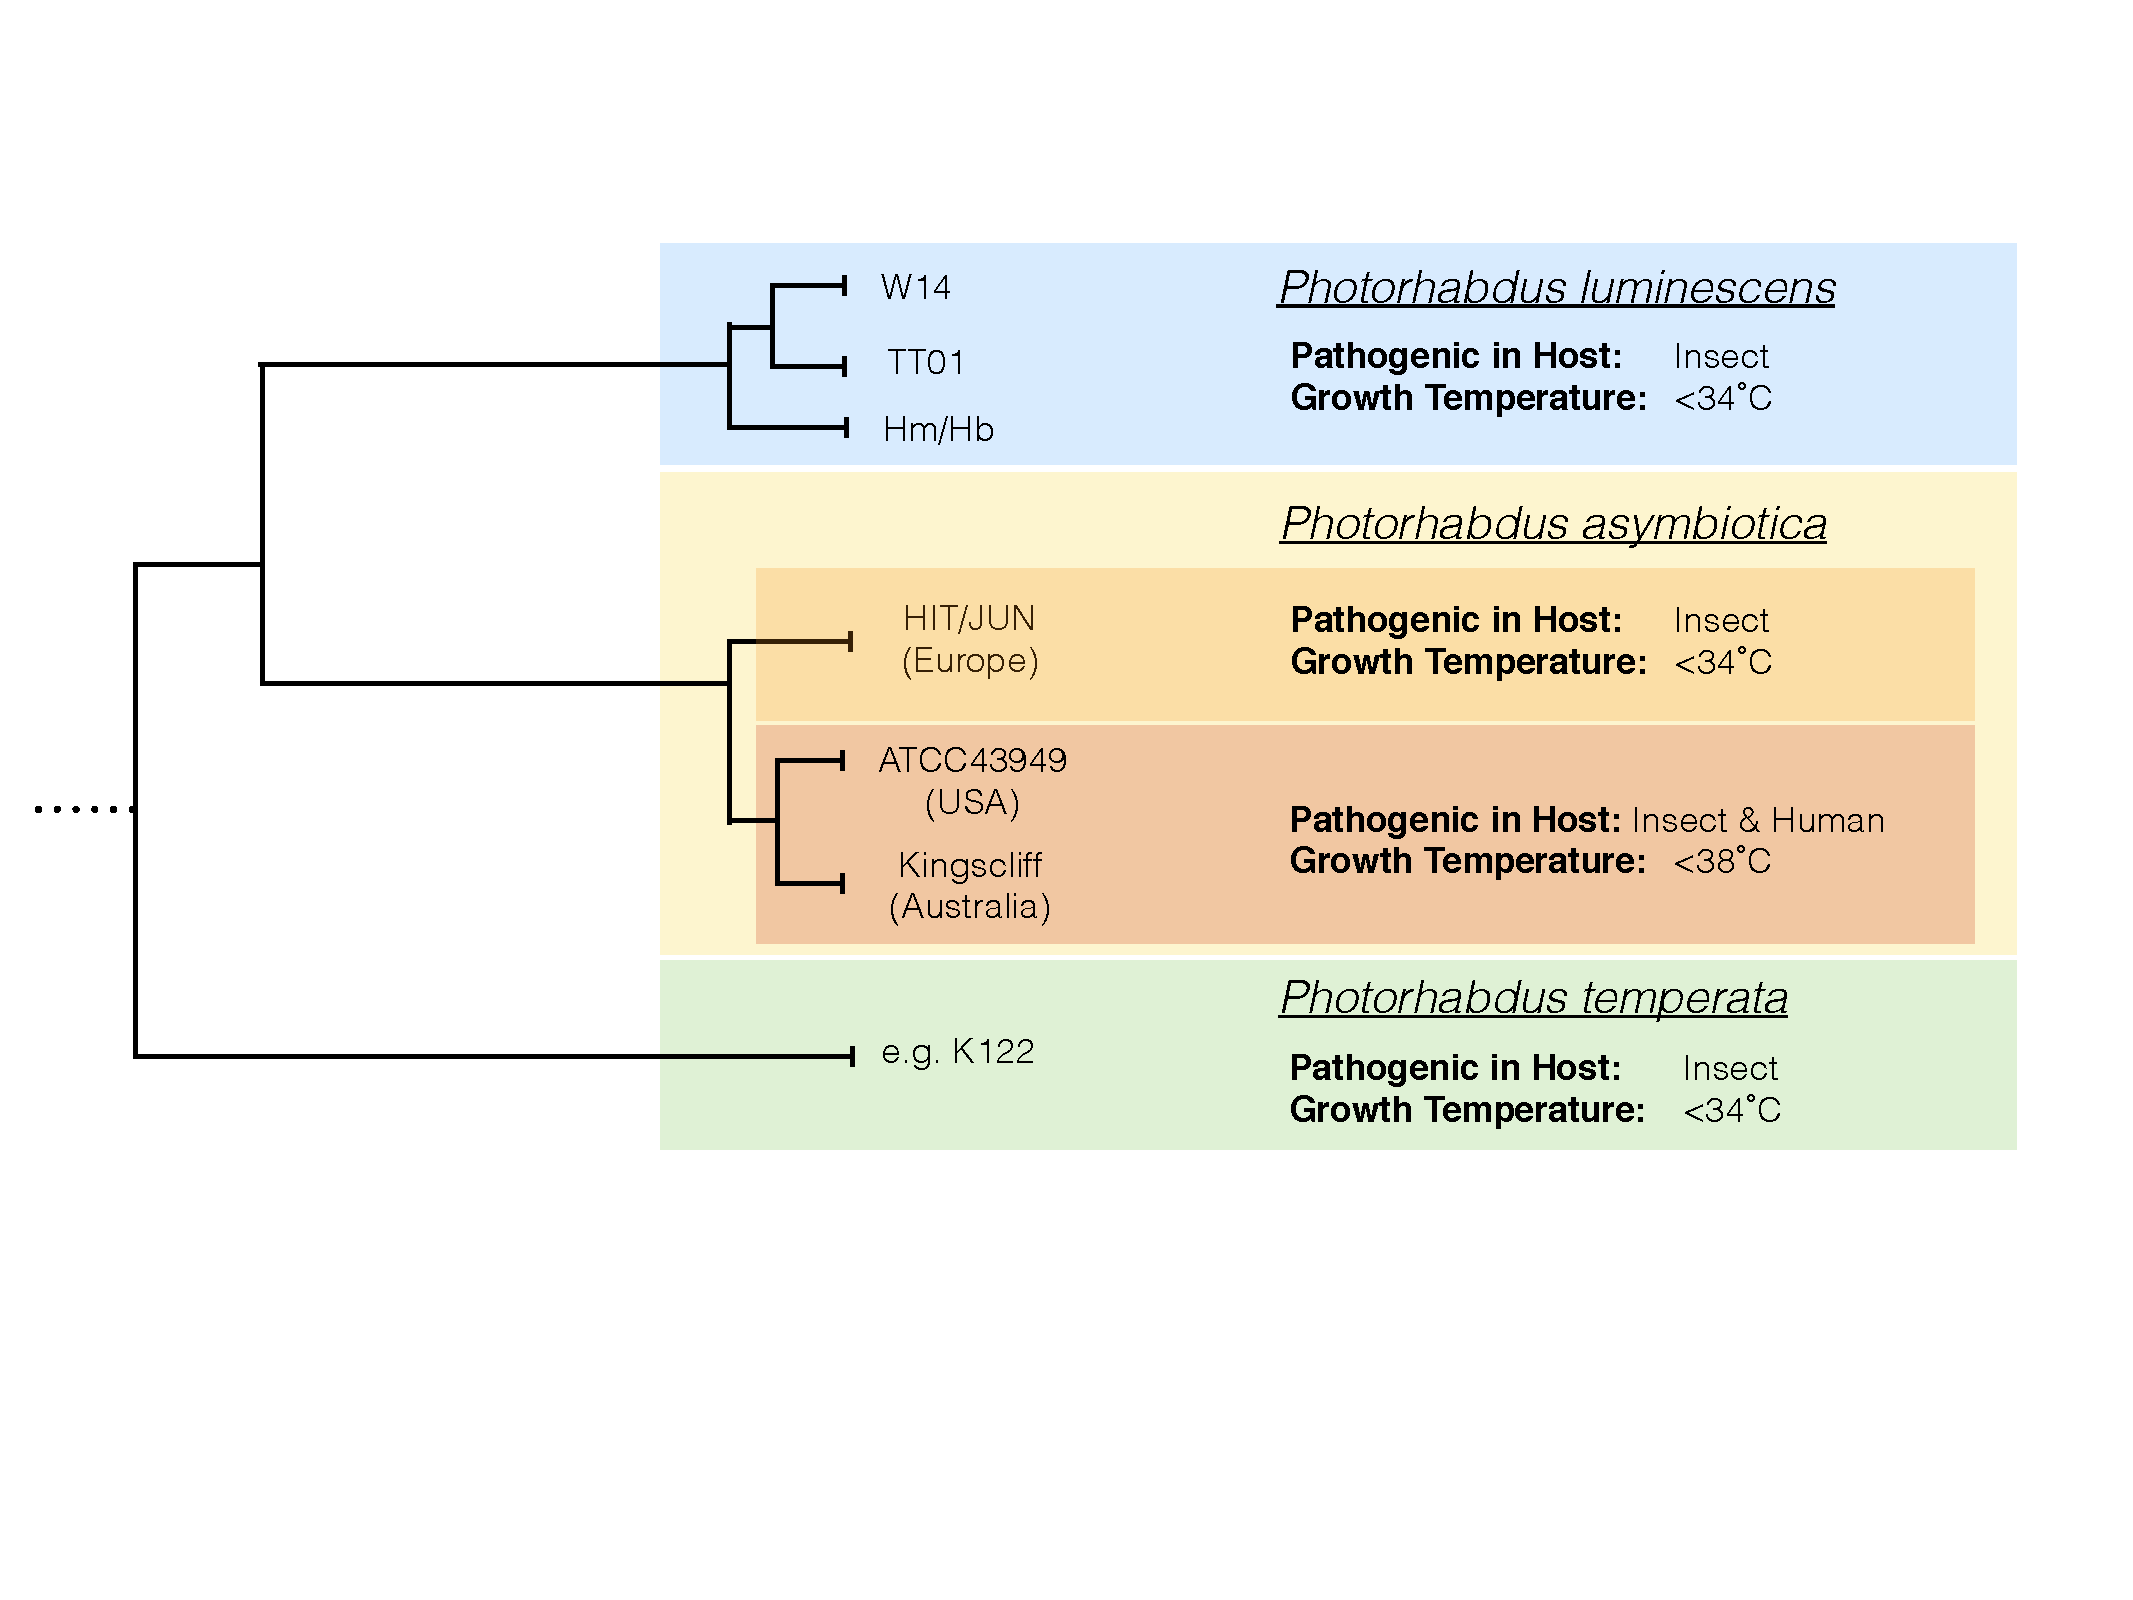
\includegraphics[width=\textwidth, clip, trim={50 180 50 110}]{/Users/joehealey/Documents/Warwick/PhD/Thesis/chapters/intro/img/lineages.pdf}
    \captionsetup{singlelinecheck=off, justification=justified, font=footnotesize, aboveskip=0pt}
    \caption[Schematic diagram of \emph{Photorhabdus} lineages]{\textsc{\normalsize A schematic diagram depicting the subclades within the \emph{Photorhabdus} genus.}\vspace{0.1cm}\newline Not drawn to scale. The schematic shows the host ranges and thermotolerance of the archetypical species within the \emph{Photorhabdus} genus, with some exemplar strains. Adapted from \citep{Waterfield2009}, and reproduced from my own Masters thesis ``\emph{Photorhabdus asymbiotica} as a Model Organism for Understanding Emerging Human Pathogens".}\label{lineages}
\end{figure}

These differences in genetic content and pathogenicity notwithstanding, all \emph{Photorhabdus} strains are obligately associated with \emph{Heterorhabditid} nematodes (see upcoming \vref{lifecycle} for a detailed explanation). Consequently, all strains must maintain the capability of associating with the host. These interactions are undoubtedly extremely complex, requiring all manner of genetic components as well as transcriptional and translational epigenetic regulation, and the molecular basis for this symbiosis is still yet to be fully understood, though some progress has been made. \Pa{} is known to exhibit a kind of phase variance, and previous studies have demonstrated that secondary phase bacteria are unable to support symbiosis, being termed ``symbiosis-deficient"; though \Pa{} phase variance appears to differ somewhat from that of other bacteria in being uni-directional \citep{Ffrench-Constant2003}. In the process of bioconversion of an infected insect, late phase \Pa{} have been shown to produce an array of secreted proteins such as proteases, toxins, and antimicrobials, to degrade the cadavers, and ward off non-\emph{Photorhabdus} competition (be it from other microbes, or from scavenging insects) \citep{Daborn2001a,Baur1998}. 

Thus, every \Pa{} strain studied to date maintains within its genome, all the symbiosis factors required for association with the nematode vector. This includes any `standard' genetic determinants, but also any regulatory and epigenetic mechanisms. All the strains also maintain virulence factors and bioconversion enzymes required to cause lethal infection and biomass conversion of an insect prey. In the case of \Pasy, they must do this in spite of a reduced genome size (though with the gain of one or more plasmids), as well as harbour all the necessary genetic apparatuses to confer infectiousness in higher order homeotherms (including, but not limited to: thermotolerance, adaptive immune resistance/evasion, facultative intracellularity). This has given rise to the hypothesis that rather than maintain a repertoire of `anti-insect' and `anti-mammalian' virulence factors etc., that instead, the virulence factors it has are efficacious against cell types from both organisms \citep{Waterfield2004a}.

\subsection{A biological `box of tricks'}
There are a number of extremely interesting and unusual aspects of \Pa{} cellular biochemistry and physiology that make it a fascinating study organism. A member of the \emph{Enterobacteriaceae}, \Pa{} is a motile, Gram negative rod shaped Gammaproteobacterium, which is partially what gives it its name: ``rhabdus" from the Greek, ``\emph{rh\'abdos}`` - ``rod" or ``wand". The former portion of its name is derived from perhaps its most striking characteristic: bioluminescence (Greek: ``\emph{ph\^os}'' - light). \Pa{} is still the only known terrestrial bacterium that exhibits bioluminescence, and does so through possession of the full \emph{luxCDABE} operon \citep{Peat2010,Clarke2008a,Farmer1989,Gerrard2003}. Why \Pa{} has maintained the operon is still a mystery, but hypotheses include use as a signalling mechanism, similar to its marine counterparts, in symbiosis (signalling to the nematode that a cadaver is populated for instance), or possibly as a virulence mechanism to deal with oxygen free radicals and enhance survival - however there is sparse evidence for these theories, and valid counters to all of them \citep{Waterfield2009}. Nevertheless, it has lead to interesting anecdotes about a phenomenon observed during the American Civil War, known as ``Angel's Glow", which has made its way in to some popular media including being covered in the well-known educational magazine ``Mental Floss" \citep{Durham2001,Soniak2012}. The phenomenon observed that soldiers who were wounded in the conflict, had a greater average survival rate if their wounds glowed. The subsequent rationale for this is that their wounds may have been infected with \Pa, which produces a myriad of antimicrobial compounds and toxins, killing off competition, including more virulent human pathogens that would have otherwise killed the individual.

The last point is another profoundly interesting and important aspect of \Pa{} biology. At the time of sequencing, it was discovered that \Pa{} has a greater proportion of its genome dedicated to secondary metabolite and toxin production than any other bacterium - including the model for secondary metabolite production, \emph{Streptomyces} (6\% vs. 3.8\%) \citep{Waterfield2009,Duchaud2003}. Among these secondary metabolites, a stilbene compound has been previously identified, \emph{3,5-Dihydroxy-4-isopropyl-trans-stilbene}, which, for a long while, \Pa{} was thought to be unique in being the only non-Plant organism known to produce it \citep{Joyce2008} - more recently it has also been detected as an \emph{Bacillus} metabolite too \citep{Kumar2013}. The compound itself has been shown to be a potent and broad range antimicrobial \citep{Hu2000}.
Consequently, the burgeoning field of `bio-prospecting' (`genome mining') \citep{Shi2018}, has begun to turn it's attention to \Pa{} as a source of novel compounds - particularly important as we continue to try and combat the threat of antimicrobial resistance \citep{Orozco2016}, and helpful as \Pa{} researchers, as it is leading to an increase in the number of available genomes and roles for many of the unknown genes. This will no doubt continue to affirm \emph{Photorhabdus}' place within the biotechnology world, complementing the exploitation which is already underway of the \emph{lux} operon, and the organism itself for biopesticides - and, we hope, the PVCs in due course.

\subsection{The life cycle of a pathogen and mutualist}\label{lifecycle}
\Pa{} is an obligate pathogen and symbiont \citep{Ffrench-Constant2003}. Much of the research interest in the organism to date has been specifically because of this unusual life style. There are abundant examples of symbiotic microorganisms and pathogenic organisms, but very few where both lifestyles are found to be exhibited by a single organism. Trying to unravel the complex molecular basis for this is a huge task, making \Pa{} an unusual and valuable emerging model.

\Pa{} is a seemingly ubiquitous soil dwelling bacterium, having been isolated from all over the world, though most commonly near coastlines. However, it is not thought to survive exposed in the soil by itself. Instead, it is found in mutualistic symbiosis with entomopathogenic soil nematodes, specifically members of the \emph{Heterorhabditidae}. In fact, such is the specificity of this mutualism, that different nematode species are known to harbour only particular bacterial species - the closely related \emph{Xenorhabdus} are associated with \emph{Steinernema} nematodes instead, for example \citep{Chaston2011}. The `bacterium-nematode complex' has potent demonstrated lethality against members of the \emph{Lepidoptera}, \emph{Coleoptera}, \emph{Hymenoptera}, and \emph{Dictyoptera} \citep{Naidoo2015}, and has been used for many years now as a biopesticide \citep{Waterfield2009}. In the soil, the bacteria are associated with the so-called ``Infective Juvenile" (IJ) (which is developmentally equivalent to the ``Dauer juvenile" of \emph{Caenorhabditis elegans}) stage of the nematode host, which is free living and actively seeking insects to infect/parasitise. 

\begin{figure}[h]
    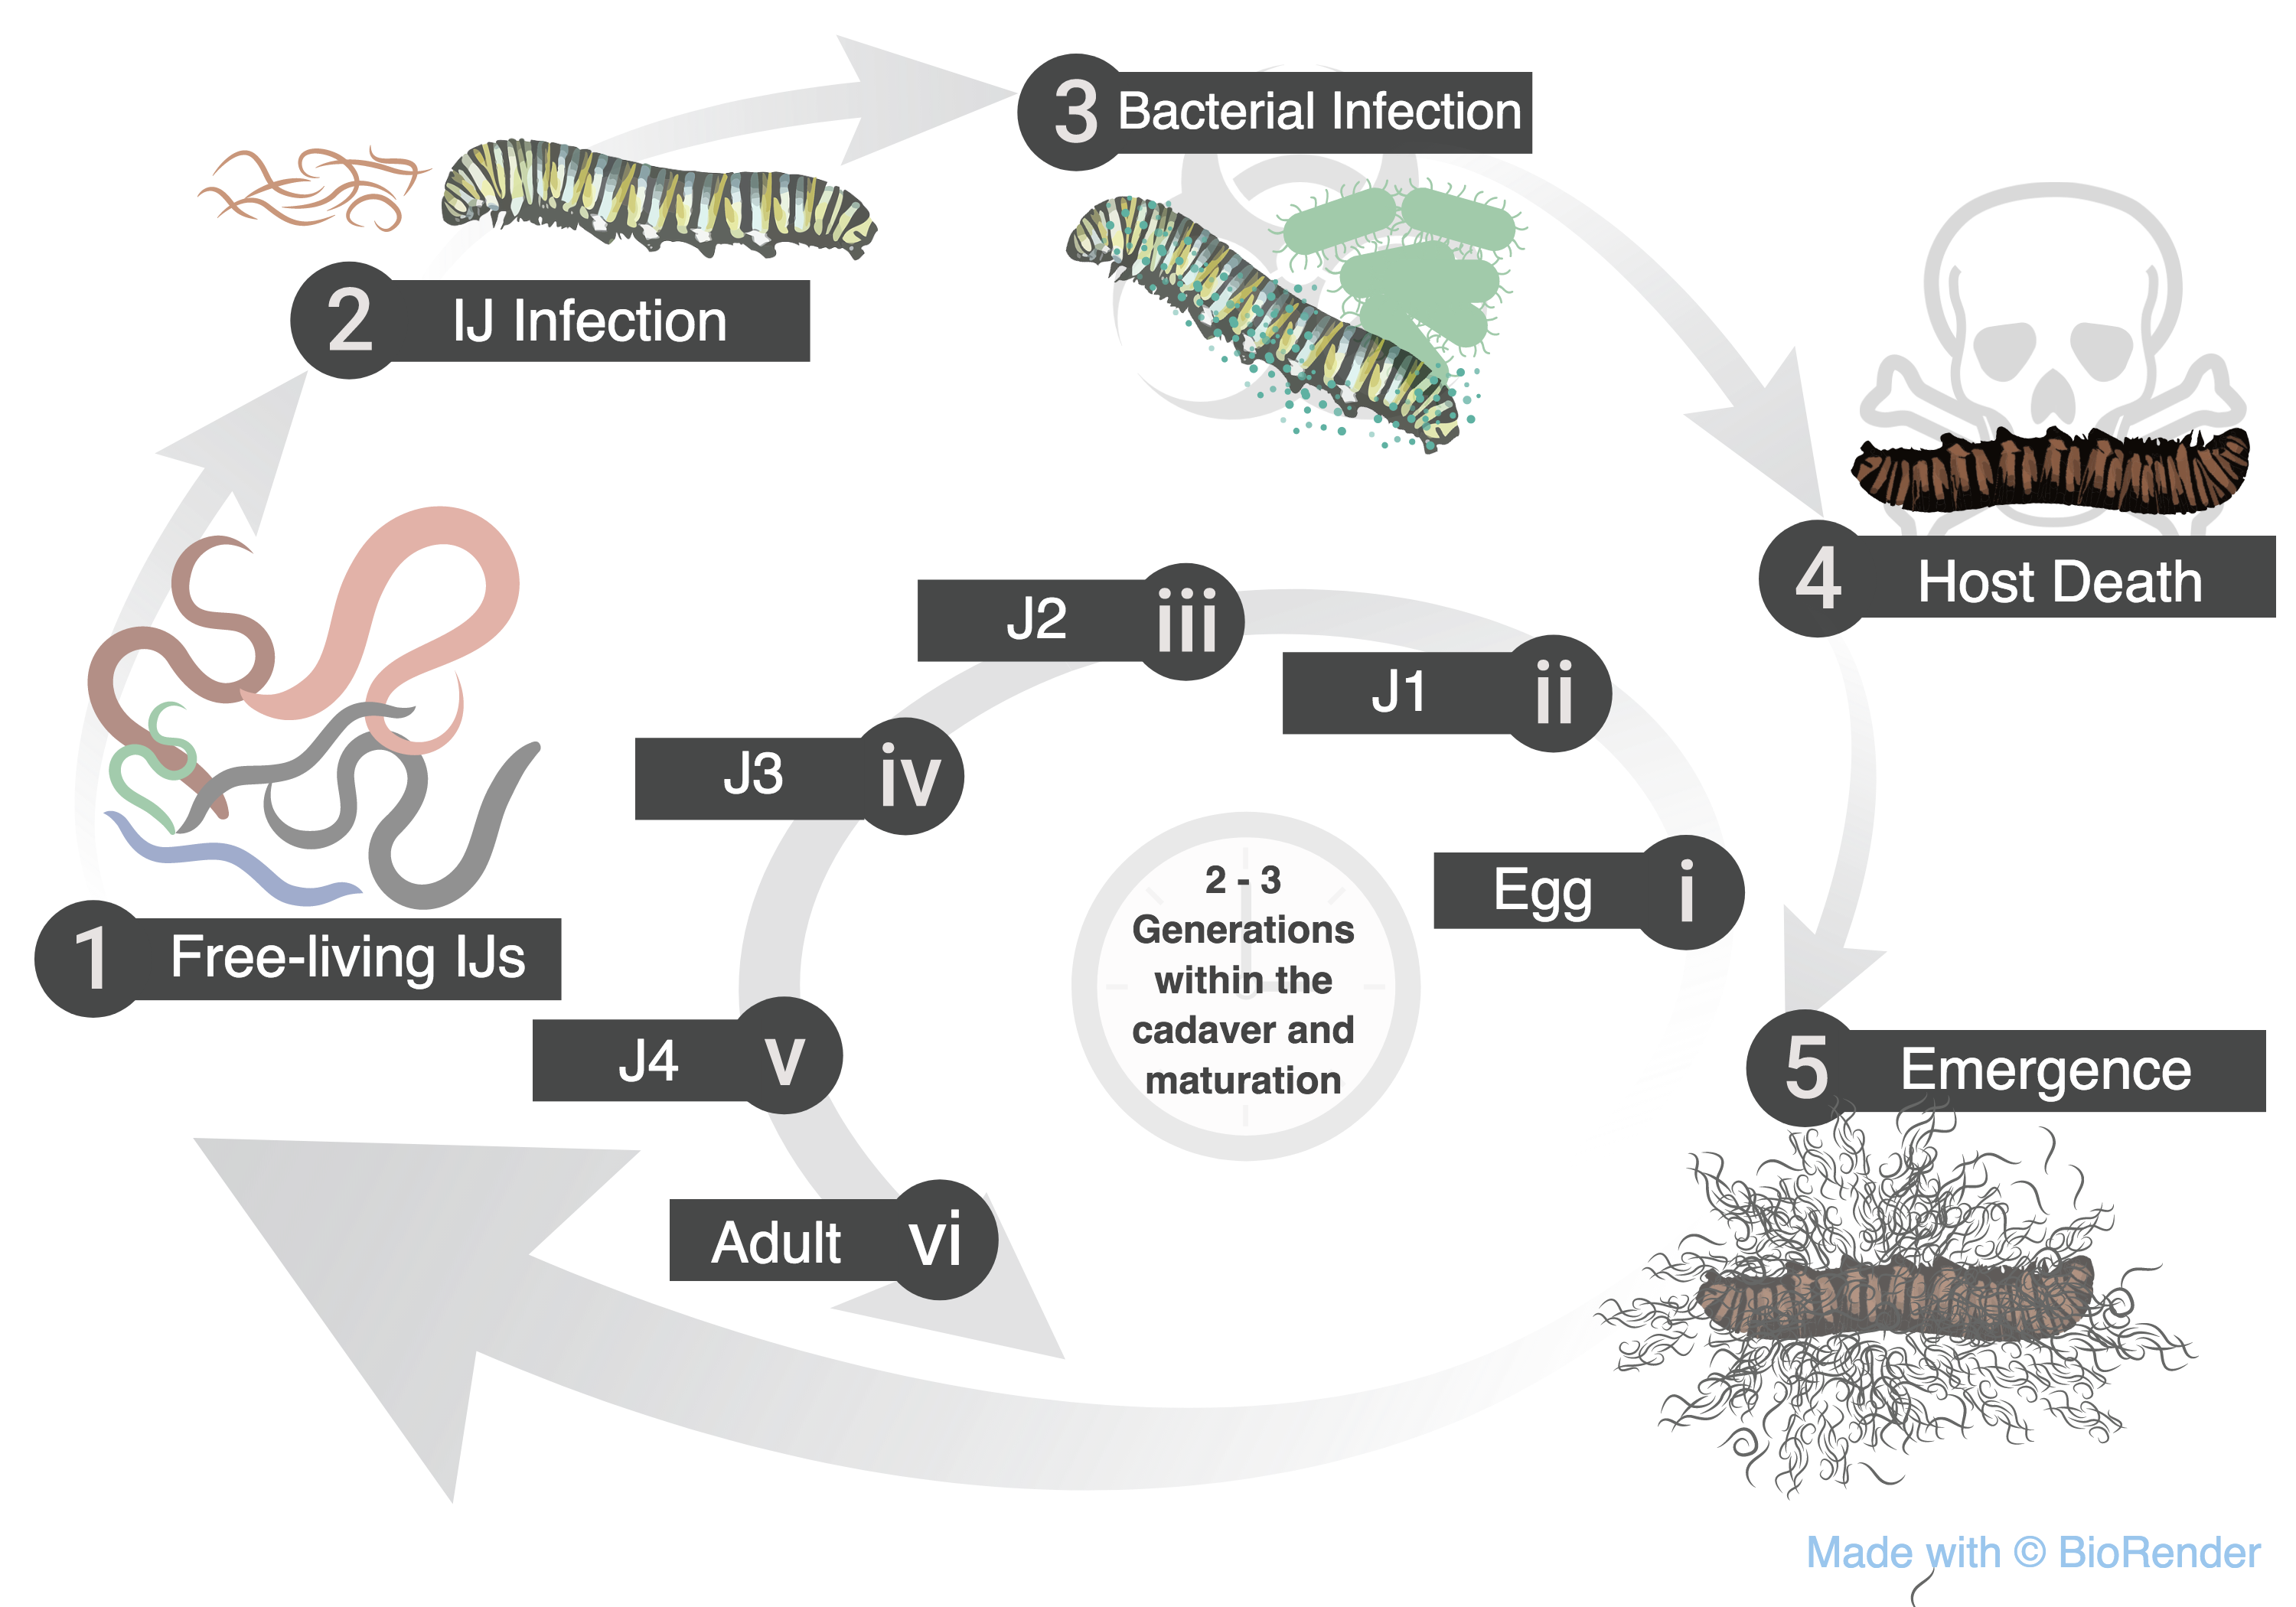
\includegraphics[width=\textwidth, clip, trim={0 25 0 0}]{/Users/joehealey/Documents/Warwick/PhD/Thesis/chapters/intro/img/lifecycle.png}
    \captionsetup{singlelinecheck=off, justification=justified, font=footnotesize, aboveskip=10pt}
    \caption[Diagram of \emph{Photorhabdus} and \emph{Heterorhabditid} nematode infection cycle]{\textsc{\normalsize The infection lifecycle of the Entomopathogenic Nematode complex.}\vspace{0.1cm}\newline
\textbf{(1)} The free living ``Infective Juveniles'' (IJs) in the soil seek out a new insect host to prey on. \textbf{(2)} IJs ingress in to the insect prey either through natural openings or boring through the cuticle. \textbf{(3)} \emph{Photorhabdus} bacteria are regurgitated by the EPN in to the open blood system of the insect (hemocoel). \textbf{(4)} The bacteria reproduce and express virulence factors to kill the prey in a matter of hours. \textbf{(5)} Bio-conversion of the cadaver biomass in to additional bacteria provides a food source for the continued reproduction of nematodes. \textbf{(i-vi)}) During replication on the cadaver, juvenile nematodes reach maturation and conduct their sexual reproduction phase. Millions of next generation IJs then leave the cadaver, reassociating with the bacteria to find the next prey insect. Adapted from \url{http://www.giabr.gd.cn/kxcb/kpdt/201405/t20140516_234014.html}, and in turn \citep{Ffrench-Constant2003}}
    
 \label{lifecyclefig}
\end{figure}

As \vref{lifecyclefig} shows, the cycle begins with free-living Infective Juvenile nematodes in the soil. The IJs are associated with their \emph{Photorhabdus} symbiotes, where the bacteria reside in the lumen of the nematode gut. Conversely, in the \emph{Xenorhabdus-Stiernema} complex, the bacteria are relegated to quiescent growth in a specialised region of the intestine known as the `receptacle'. IJs are a specialised alternative third developmental stage which are non-feeding, self-fertile hermaphrodites, with increased resilience to environmental stresses (by retaining an additional cuticle layer \citep{Ciche2003a}). IJs seek out prey insects within the soil to parasitise, and enter the organisms open circulatory system (or ``hemocoel'') via natural openings such as the spiracles (breathing tubes), mouth or anus. Alternatively, the nematodes bear a sharp tooth-like structure at the mouth which they can use to bore through the cuticle of the organism. Once inside, the nematodes regurgitate their bacterial `payload', which is typically less than 200 individual cells, speaking to the potency of the entomopathogenic activity of \emph{Photorhabdus}, which then employ sophisticated molecular tools to evade the immune response and establish an infection. The regurgitation and triggering of developmental processes for the nematode are induced by compounds within the insect hemolymph (blood) \citep{Ciche2003a}. Interestingly, the same paper by Ciche and colleagues showed that Grace's insect medium could not replicate this effect, suggesting that it is only very specific compounds involved in the process which are not reproduced in artificial media, though these compounds could not be identified specifically. Over the course of the next $\approx$36 hours, the IJs developmental switch, brought about by the insect environment, triggers feeding behaviour. The bacteraemia is lethal to the host insect, due to rapid proliferation and production of many exoenzymes and virulence factors. The bacteria therefore digest and bioconvert the cadaver, and the nematodes feed on the new bacterial biomass. Some of the ingested bacteria adhere to the nematode intestine and invade the rectal gland cells, restoring the EPN complex. While growing and maturing on the insect cadaver, the nematodes can complete their maturation to adults, having been larval juveniles up to this point. Their development to adults also leads to a dioecious stage, rather than the hermaphroditic one seen in the IJs, meaning that the nematodes can undertake sexual reproduction. Once the cadaver is exhausted, the EPN complexes vacate the site and go off in search of fresh prey, repeating the cycle.

There are a number of theories suggesting a basis for the control of symbiosis and the switch to pathogenicity (though a full review is beyond the scope and need of this thesis), including the use of the \emph{lux} operon as mentioned earlier, and recent studies have shown that many of the secondary metabolites that \Pa{} produces have roles in this mechanism. It has been observed that mutants in \emph{relA} and \emph{spoT}, which are both ppGpp alarmone synthases, become deficient in secondary metabolism and in symbiosis, but not in virulence \citep{Bager2016}. Mutants in the malate dehydrogenase enzyme (\emph{mdh}), exhibited similar behaviour, with no effect on virulence, but becoming incapable of mutualism (and unable to produce light, pigments, and the previously mentioned stilbene compound; all of which are hallmarks of post-exponential phase secondary metabolism). \emph{mdh} is a central enzyme in the Krebs' Cycle, implicating it in both central and secondary metabolism \citep{Lango2010}. Similarly, mutants in \emph{hfq}, a global post-transcriptional regulator that is widespread in bacteria demonstrated complete abolishment of all known secondary metabolite production, and a concomitant failure to associate with the nematode vector \citep{Tobias2016}. Large-scale lifestyle decisions, such as sporulation in \emph{Bacillus}, a process thought to involve as much as half of the genome, may be analogous. Certainly, there are similarities in that both processes require a functional Krebs' cycle \citep{Stephens1998}, and so it seems likely that a complex process such as symbiosis could also involve a significant proportion of the genome. It is probable, therefore, that any or all of the aforementioned theories are true, and that there are a vast number of pathways working together to fettle and control the symbiosis and pathogenicity process.

%\section{Toxins and Virulence Factors of \Pa}
%As this thesis primarily concerns a toxin system of \emph{Photorhabdus}, a little more time will now be dedicated to discussing the dizzying array of toxins/virulence factors which the bacteria puts to use, before discussing the PVCs specifically. Mounting information on the structure and biological activity of many of the toxins from \emph{Photorhabdus} is only serving to reinforce the earlier assertion that the genus harbours a greater number and diversity of toxic entities than seen in any other genus of microorganism to date, and thus there are interesting evolutionary pressures acting to maintain what, would at first glance, appear to be a genome of high redundancy \citep{Richard2014a}.
%
%\subsection{Mcf}
%\subsection{Pir}
%\todo[inline]{populate this section}
%
%\subsection{The ``Tc" Toxins}
%One of the earliest discoveries, which has spurred a significant amount of \emph{Photorhabdus} research, was the identification of the orally active ``Tc" system \citep{Bowen1998}. Taking their name literally from ``Toxin Complexes", the Tc's are formed from 3 separate components - TcA, TcB and TcC. The structure, which was recently resolved in atomic detail \citep{Meusch2014}, shows that TcA multimerises in to a striking, inverted bulb-like, or vase shape, and the whole complex is on the order of a megadalton. The pentameric TcA complex is a staggeringly elaborate cell surface binding and payload ejection system. An entropic spring chain of amino acids that stretches across almost the length of the entire structure keeps it poised such that upon binding to the cell an outer shell is retracted, revealing an extended helical central channel which is forced into the membrane, creating a pore. TcB and TcC sit atop the `vase' like structure forming a so-called ``cocoon", comprised mostly of a $\beta$ sheet cage-like structure with a hollow interior. In early study, it was observed that the TcA gene could be expressed alone, but TcB and TcC had to be expressed together, and only when all 3 components were reconstituted together was oral toxicity restored \citep{Richard2014a, Waterfield2001z, Sergeant2003}.  The toxic moiety of this enormous complex is contained within the TcC protein, but interestingly, the protein is not dedicated to just being a toxin, forming half of the `cocoon' that was just mentioned. In fact, the TcC C-terminus is cleaved off by the TcB, meaning that both perform catalytic as well as structural roles. Physicochemical properties of the interior of the cocoon mean that the cleaved C-terminus moves in to the lumen of the pre-pore within the centre of the TcA pentamer. Upon binding to the cell, the enormous conformational change that occurs in the TcA, penetrating the membrane, allows the toxic subunit free passage to the cytosol. Meusch and colleagues make the interesting observation that TcC are hyper-variable, meaning that there is the potential to delivery a diversity of toxin `payloads' \citep{Meusch2014}. It has also been noted that the \Plum{} TcB/C complex shares only around 56\% sequence identity with the homologous structures in \emph{Yersinia entomophaga}, despite elaborating almost identical tertiary and quaternary structures \citep{Richard2014a}. This diversity of sequence, yet conservation of structure/function, has lead to these complexes being termed `polymorphic toxin systems', along with the PVCs \citep{Zhang2012a}. These systems are characteristically highly recombinant, particularly in the types and modes of actions of their payloads, and this is an important point worth bearing in mind for much of this thesis. Under this nomenclature, both the Tcs and the PVCs are classified with the type II, V, VI and VII secretion systems, among others.
%
%
%This just goes to show the ingenuity \Pa{} (and many other related bacteria) are exhibiting when creating highly effective and staggeringly complex toxin systems - a fact that will be all the more apparent shortly when the PVCs are introduced fully.

\section{The \Pa{} Virulence Cassette}
Not much is known for certain when it comes to the \Pa{} Virulence Cassettes, and even less has been published. To date, there has only been a single paper on the discovery and biology of the \emph{bona fide} PVCs \citep{Yang2006}. However, an increasing number of papers have appeared, particularly in the last $\approx$5 years, which have attempted to understand how PVCs `fit in', in a wider context, and have begun to speculate on the roles of various genes. While there is nothing wrong with this in principle, much of the biology is still lacking, and it is not always constructive to try and constrain a biological entity to fit within the criteria for different systems. With the rapid proliferation of structural data for analogous systems however, thanks in no small part to the advancements in cryo-electron microscopy for studying large macromolecular complexes, there has never been a better time to study fascinating structures such as these.

As these structures are complex, multipartite and still quite enigmatic, this section will serve as a `guided tour' through the various components of the PVC structures, as well as draw analogies against other, better characterised, related structures as it was understood before this project began, to help the reader understand the chapters to come. \vref{structbioinfo} will continue in this vein, in the context of what has been learnt since, with the advantages of more complete databases and a better biological understanding, to fill in some of the gaps.

\subsection{Discovery of the PVCs}
Upon sequencing of the first \emph{Photorhabdus} genomes, the PVCs were identified as putative prophage regions the \Plum{} TT01 genome, in 4 tandem repeats which demonstrated unusual \% GC content. When a cosmid library was constructed from the \Pasy{} ATCC43949 genome, clones harbouring the operon for a particular PVC with the so-called `Pnf' (\emph{Photorhabdus} necrosis factor) cognate effector demonstrated high levels of injectable toxicity against whole insects - killing them in as little as 15 minutes, and earning them their name (``Virulence Cassettes") \citep{Yang2006, Waterfield2008}. It became apparent from these early experiments that the PVCs represented a novel kind of toxin delivery and translocation mechanism, and similar patterns of toxicity could be identified in other cosmid clones which bore other PVC variants. The Pnf effector of this particularly potent PVC, is homologous to the active site domain of Cnf1 (Cytonecrosis Factor) of uropathogenic \emph{Eschericia coli}, and works in the same way, by activating Rho GTPase proteins inside the target cell, which leads to cytoskeleton depolymerisation \citep{Landraud2004, Buetow2001}. Further inspection showed this cosmid to contain what we have now come to recognise as a PVC, with its associated effector, and several more cosmids within the library were identified which contained various other PVCs. It was observed that a number of the cosmid-borne PVC operons are defective in some way, suggesting that the obtained colonies were those where the cosmids had been inactivated in some way such that they could be tolerated. This potential self-toxicity is the subject of \vref{regulation}.

The PVCs were able to be purified/enriched from the cosmid supernatants to identify the basis of the toxicity, using diethylaminoethyl-sepharose resins and upon imaging via electron microscope, sure enough, phage like structures were apparent in the samples. Subsequent immunogold staining using antibodies raised against the Pnf toxin showed that, when disrupted, the structures appeared to be loaded with the toxins. \vref{PVCems} shows some of the original microscopy, reproduced from the \cite{Yang2006} study, as well as some more recent micrographs from the lab and an ongoing collaboration with the Max Plank Institute in Dortmund, showing cleaner samples. Preliminary data from the collaboration with the Max-Planck Institute resolving the atomistic structure of the PVCs is now beginning to vindicate the many assumptions about the PVC architecture, biology and function.

\vspace{0.1cm}
\begin{figure}[h]
\centering
    \begin{subfigure}[b]{0.33\textwidth}
        \centering
        {%
\setlength{\fboxsep}{0pt}%
\setlength{\fboxrule}{1pt}%
        \fbox{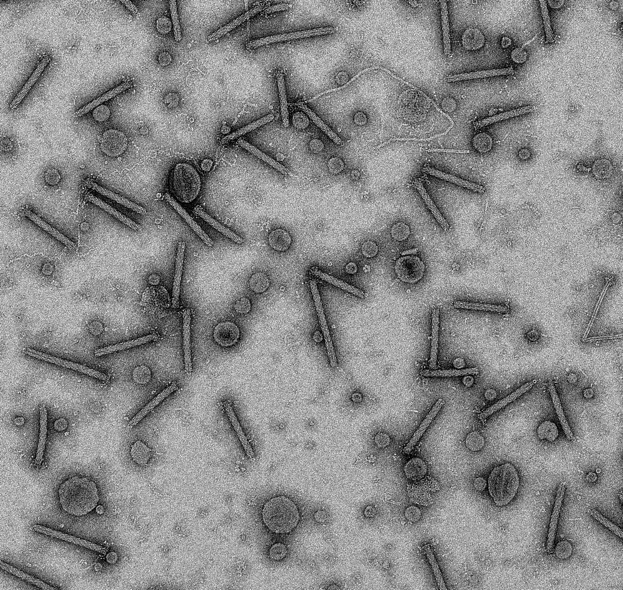
\includegraphics[width=\textwidth, trim={20 40.5 0 60}, clip]{/Users/joehealey/Documents/Warwick/PhD/Thesis/chapters/intro/img/PVCEM1.png}}
            }%
    \end{subfigure}%
    \begin{subfigure}[t]{0.33\textwidth}
        \centering
        {%
\setlength{\fboxsep}{0pt}%
\setlength{\fboxrule}{1pt}%
        \fbox{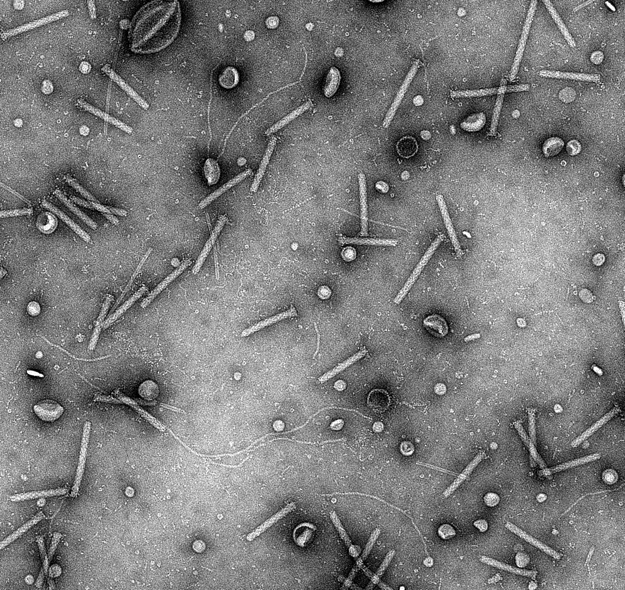
\includegraphics[width=\textwidth, trim={20 100 0 0}, clip]{/Users/joehealey/Documents/Warwick/PhD/Thesis/chapters/intro/img/PVCEM2.png}}
        }%
        \end{subfigure}%
    \begin{subfigure}[t]{0.33\textwidth}
        \centering
        {%
\setlength{\fboxsep}{0pt}%
\setlength{\fboxrule}{1pt}%
        \fbox{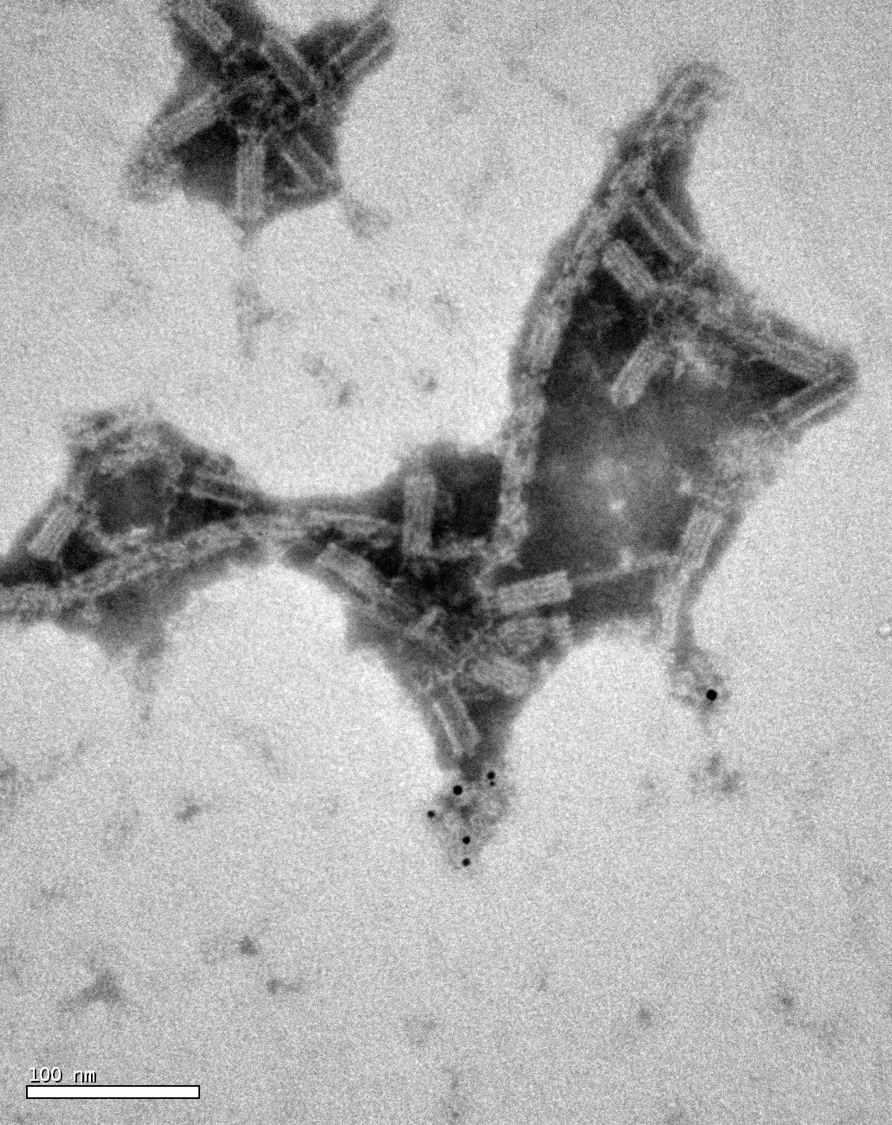
\includegraphics[width=\textwidth, trim={0 120 40 165.5 }, clip]{/Users/joehealey/Documents/Warwick/PhD/Thesis/chapters/intro/img/PVCEM3.png}}
        }%
    \end{subfigure}%

\captionsetup{singlelinecheck=off, justification=justified, font=footnotesize, aboveskip=10pt}
\caption[PVC Electron Micrographs]{\textsc{\normalsize A selection of electron micrographs of the PVCs.}\vspace{0.1cm} \newline A selection of micrographs are shown here revealing their caudate structure and the resemblance to other contractile tail systems. The left and centre panels show more recent, but unpublished data from an ongoing collaboration with the Max Planck Institute at Dortmund, purified via Cesium Chloride buoyant density gradient ultracentrifugation. The right hand panel shows one of the earliest images of the PVCs ever obtained, via diethylaminoethyl sepharose resin elution (the white mass in the background). The black dots in the bottom-center of this panel correspond to immunogold antibody staining against the payload molecules released from the syringes.}
\label{PVCems}
\end{figure}


\subsection{\Pa{} is a PVC addict}
A single PVC is a remarkable biological entity. However, \emph{Photorhabdus} has chosen not to stop here. Within the genomes studied to date, there are as many as 6 distinct PVC operons, each with 1 or more associated toxin effectors, in any single genome. The fact that each one has a hallmark effector or effectors has been used since their discovery to delineate which PVC is under discussion \citep{Yang2006} - with some exceptions. In several cases, the PVCs were simply named for their positions in the genome. Specifically, in \Plum{} TT01, the 4 tandem PVCs mentioned in the previous section were simply named ``Unit1", ``Unit2", ``Unit3", and ``Unit4". In \Pasy {} genomes, there is also a distinct ``Unit1", but confusingly, it is not most homologous to the ``Unit1"s of \Plum, being in fact, primarily orthologous to the \Plum{} TT01 ``Unit 4".

With this in mind, this is an ideal moment to briefly explain the nomenclature that will be used throughout this thesis when referring to the PVCs. The PVC with the cognate Pnf toxin that was mentioned in the previous section will be used as an example. In order to denote each PVC, the nomenclature ``PVCPnf" will be used. Where a distinction between inter-strain variants of the same operon is required, this will be followed by the strain name itself, as in: ``PVCPnf ATCC43949" or ``PVCPnf Kingscliff". Furthermore, when a specific gene is under discussion, ``PVCPnf" will be followed by the numerical identifier for that gene; so for the first protein of the \Pasy{} ATCC43949 strain Pnf operon, the nomenclature will become: ``PVCPnf1 ATCC43949". In cases where this thesis refers to just a specific locus, across all operons, the terminology will simply be ``PVC1" - i.e. the first locus, in all operons syntenically.

\vref{pvcvariants} demonstrates the variants from the \Plum{} TT01 and \Pasy{} genomes. The existence of phage-like contractile tails in a myriad of genomes has now been demonstrated, however, \emph{Photorhabdus} appears to remain somewhat unique, in that no other organisms have been found, so far, which harbour so many forms of the same structure in a single genome. Even if one examines \emph{Xenorhabdus} strains, which are as closely related as it is possible to be outside of the immediate \emph{Photorhabdus} genus, it is only possible to identify single copies of PVC-like operons.

\begin{figure}[p]
	\thisfloatpagestyle{IHA-fancy-style}
	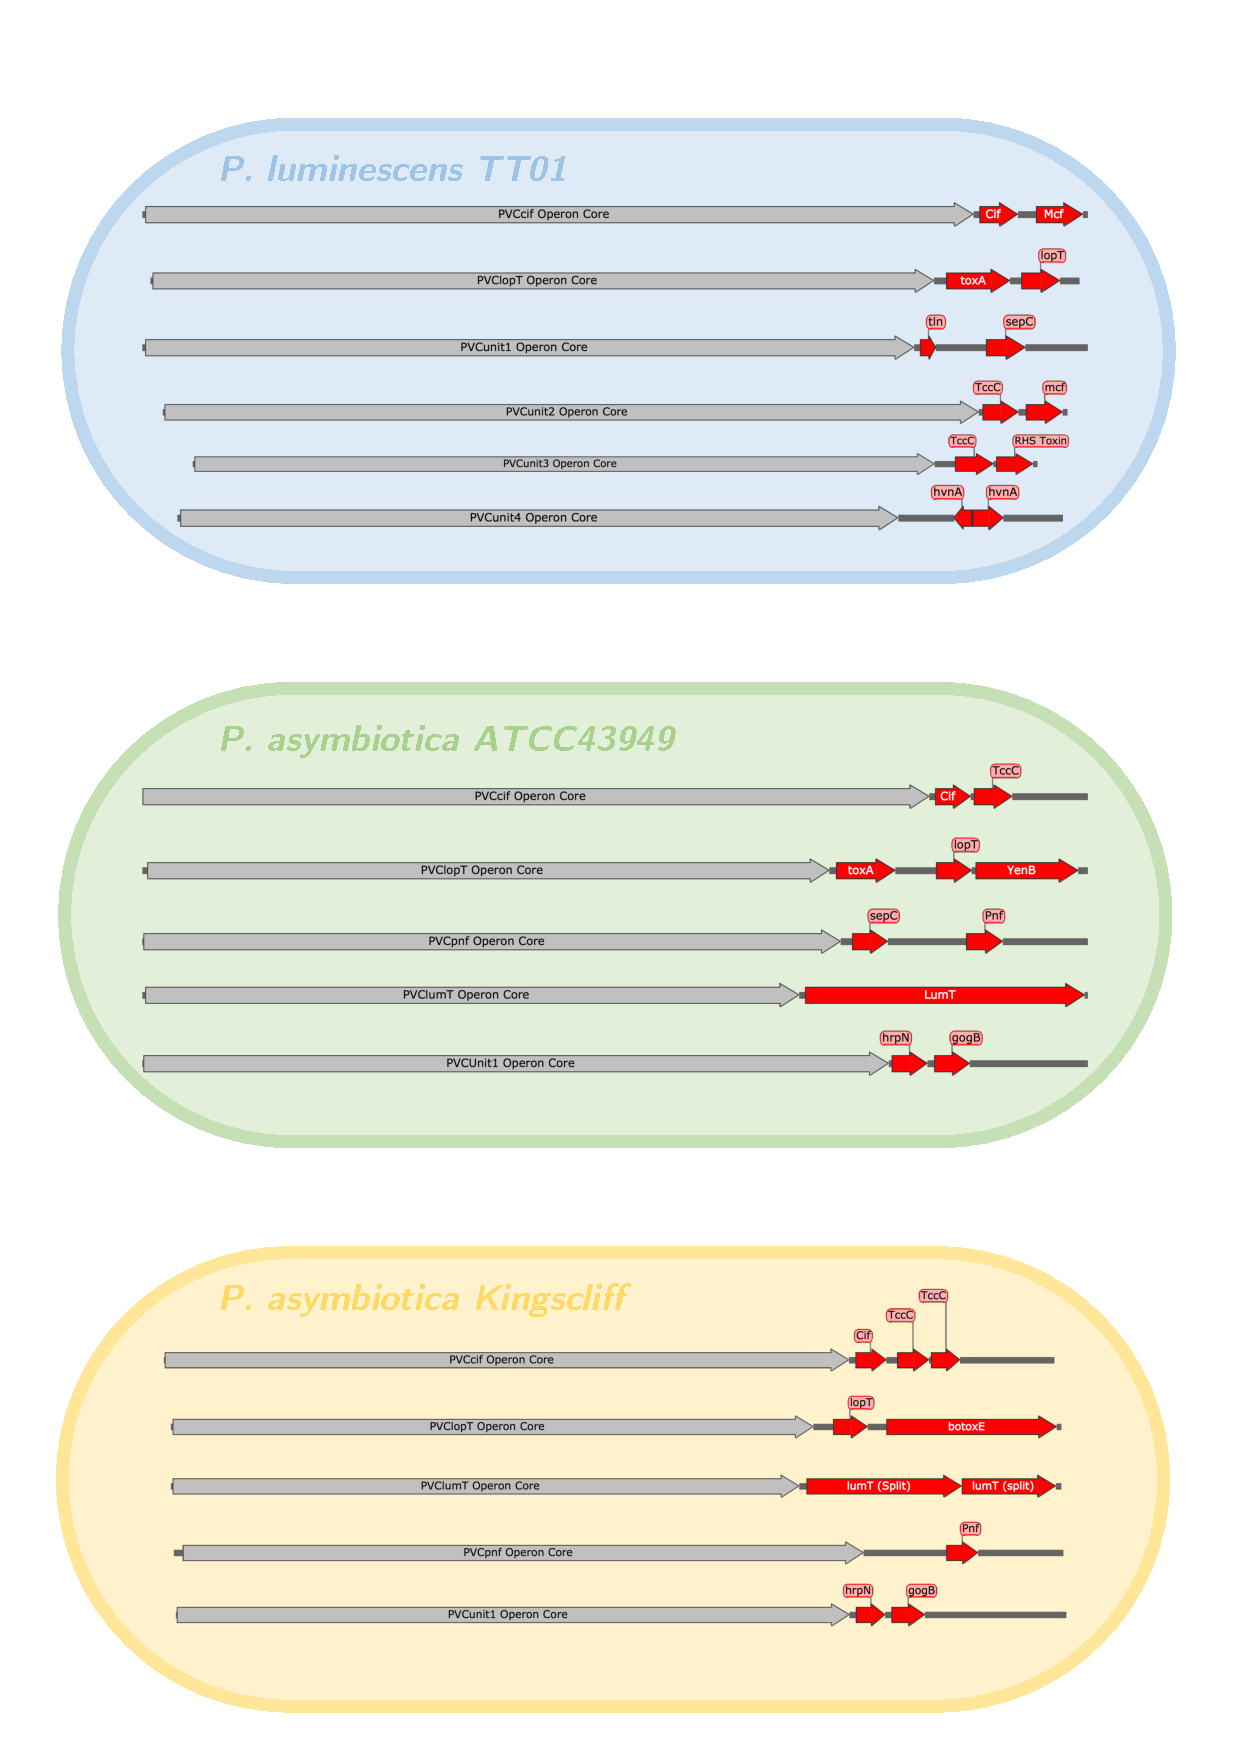
\includegraphics[width=\linewidth, clip, trim={25 10 26 55}]{/Users/joehealey/Documents/Warwick/PhD/Thesis/chapters/intro/img/hostofhostsfig.pdf}
	\captionsetup{singlelinecheck=off, justification=justified, font=footnotesize, aboveskip=5pt}
	\caption[Schematic of PVC variants across 3 \emph{Photorhabdus} genomes]{\textsc{\normalsize The PVC variants found in 3 \emph{Photorhabdus} genomes.}\vspace{0.1cm} \newline A schematic of the variant forms of PVCs found in the 3 different genomes this thesis will focus on. The operon core is denoted in a single grey arrow, and the diverse effector proteins which distinguish the operons are identified in red. Individual operons are to scale, however the scale between operons is not identical; they are all approximately 23 - 25 kbp.}
	\label{pvcvariants}
\end{figure}

Naturally, this leads to questions about how and why \emph{Photorhabdus} is able to maintain so many copies of operons which have a high degree of internal and inter-operon paralogy. Conventional wisdom would suggest that at least 1 of these extra operons might drift to the point of removal/pseudogenicity. For certain, there are substantial genetic differences between different PVCs, and drift has most likely played a part in this, but nevertheless they persist, which suggests the selective pressure is sufficient on each PVC to maintain them. There are a few speculative rationales that this could be the case. Firstly, it's possible that \emph{Photorhabdus}' life cycle is so competitive that any additional toxin systems of a net benefit to the organism, despite their high metabolic cost, with each fulfilling sufficiently different roles. This would further mesh with the observation that \emph{Photorhabdus} elaborates the largest repertoire of toxins known so far. An alternative idea however is that not all PVCs are evolved with a toxic effect in mind, and may have host modulatory effects - which will be covered in more detail in a later section. There is some preliminary evidence that different PVCs perform different roles, perhaps with toxicity to particular tissue/cell types, or responding to different environmental cues.

This almost paradoxical variability-yet-conservation is a recurring theme in this thesis, and is also useful for understanding any single one of the PVCs.



\subsection{PVCs as contractile nanomachines}
The initial electron microscopy, and homologies observed to R-type pyocins \citep{Ge2015}, the Antifeeding prophage \citep{Heymann2013},  and other prophage sequences, which have had their structures resolved or electron microscopy (EM) studies conducted, provided compelling evidence that the PVCs elaborated a similar caudate structure. Moreover, it has become increasingly apparent in recent years that the entire mechanism of `contractile machines' is an evolutionarily conserved structure which appears time and time again in nature - and not just in the form of prophages, which is what many of these devices have been mistaken for to date \citep{Kube2015a, Sarris2014, Brackmann2017}. In particular, in the Sarris et al. paper, contractile tail mechanisms of various forms have been demonstrated to be widespread with a remarkable diversity of functions, even in the Archaea. Much as the bacteriophage biosphere has become increasingly well understood to actively shape the bacterial biosphere, it is now becoming similarly apparent that phage-like structures will have had (and are having) a similarly decisive role in shaping ecosystems and evolution \citep{Richard2014a}. The following sections now detail the state of knowledge for the well studied cousins of PVCs; readers are also encouraged to look at the original Kube and Wendler, Taylor et al., and Sarris et al. papers for 3 excellent reviews from both a structural and genetic perspective \citep{Kube2015a, Sarris2014, Taylor2018}.

\subsubsection{Of PVCs and Phage}
Contractile tail nanomachines are typified by the bacteriophage order \emph{Caudovirales} (from the Latin: ``\emph{cauda}" - ``tail"), so it makes sense to start here. In particular, those of the \emph{Myoviridae} family, to which the well known model T4 phage belongs \citep{Ackermann1998}. Phages have been studied for over 100 years now, after their original discovery at the beginning of the 20th Century by F\'elix d'H\'erelle \citep{DHerelle1917}. d'H\'erelle is also credited with conceptualising phage therapy, which is becoming increasingly relevant again with the rise of antibiotic resistance.

The tail structures of the T4 bacteriophage were the first structures ever to be resolved by electron microscopic (EM) density reconstruction as far back as 1975 \citep{Amos1975}; and with the recent explosion of Cryo-EM data, and the so called ``Resolution Revolution" \citep{Kuhlbrandt2014}, we have a clearer understanding of these elegant and staggeringly complex macromolecular machines than ever before. The tail tube, capsid, and the intricate baseplate complex of T4 have now been solved to atomic or near atomic resolution \citep{Aksyuk2009, Kostyuchenko2003, Kostyuchenko2005, Fokine2004, Fokine2013, Rossmann2004, Taylor2016b, Lan2014}, and is probably the single most well studied structural entity. \vref{t4EMs} shows some of the actual micrographs of T4 collected to date, and \vref{t4structure} shows a collection of the now resolved structures reproduced from the literature. Even at a glance, its quite apparent that these entities share similar origins and architectures.

\vspace{0.1cm}
\begin{figure}[h]
\centering
    \begin{subfigure}[b]{0.41\textwidth}
        \centering
        {%
\setlength{\fboxsep}{0pt}%
\setlength{\fboxrule}{1pt}%
        \fbox{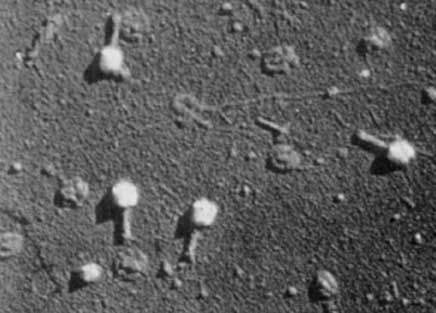
\includegraphics[width=\textwidth, trim={0 0 0 74.2}, clip]{/Users/joehealey/Documents/Warwick/PhD/Thesis/chapters/intro/img/EM_of_phage_T4.jpg}}
            }%
    \end{subfigure}%
        \begin{subfigure}[t]{0.16\textwidth}
        \centering
        {%
\setlength{\fboxsep}{0pt}%
\setlength{\fboxrule}{1pt}%
        \fbox{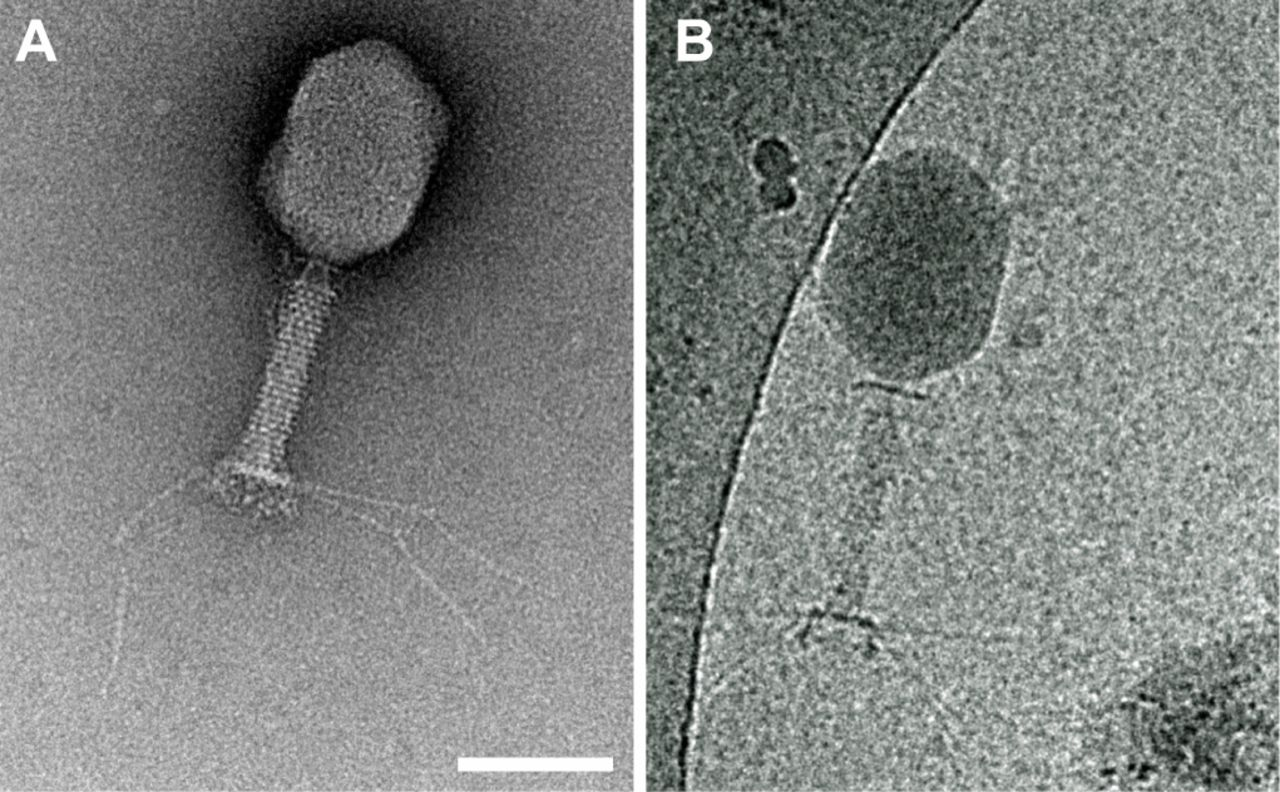
\includegraphics[width=\textwidth, trim={20 40 180 0  }, clip]{/Users/joehealey/Documents/Warwick/PhD/Thesis/chapters/intro/img/isEMdead.jpg}}
        }%
    \end{subfigure}%
    \begin{subfigure}[t]{0.41\textwidth}
        \centering
        {%
\setlength{\fboxsep}{0pt}%
\setlength{\fboxrule}{1pt}%
        \fbox{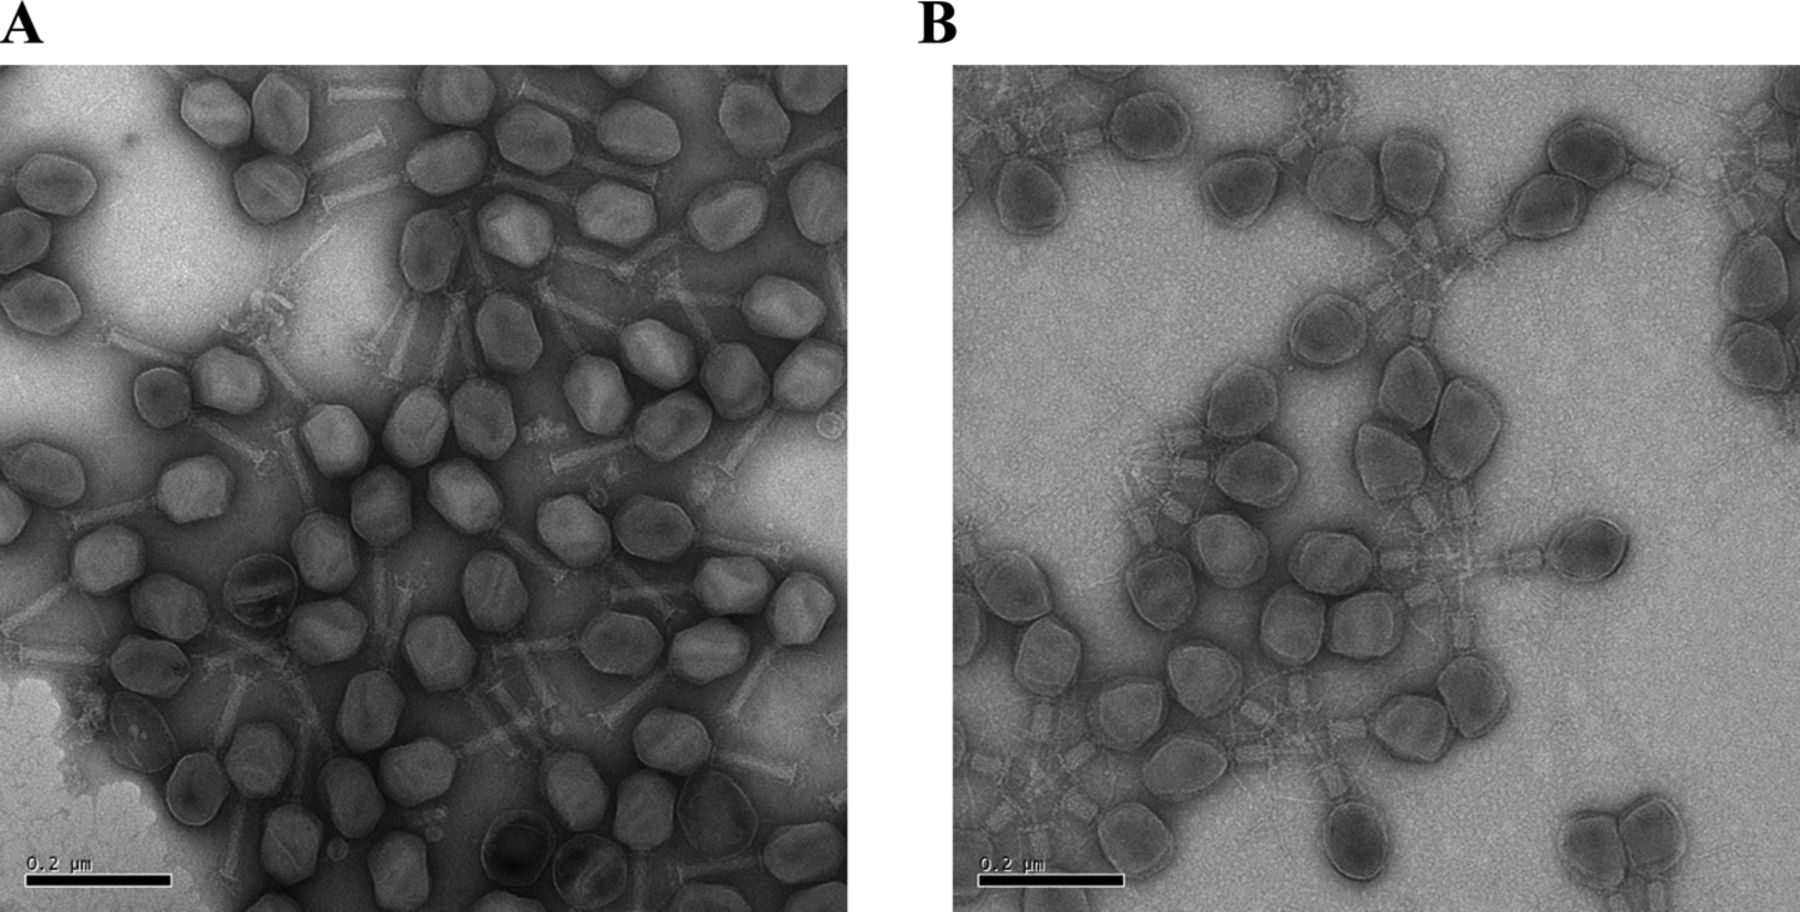
\includegraphics[width=\textwidth, trim={0 50 240 64}, clip]{/Users/joehealey/Documents/Warwick/PhD/Thesis/chapters/intro/img/EMlargescale.jpg}}
        }%
        \end{subfigure}%
	\captionsetup{singlelinecheck=off, justification=justified, font=footnotesize, aboveskip=10pt}
	\caption[Electron micrographs of Bacteriophage T4]{\textsc{\normalsize Electron Micrographs of T4 bacteriophage virions.}\vspace{0.1cm} \newline The left panel shows an early T4 phage micrograph from 1958, reproduced from \url{https://www.molbio.unige.ch/eng/about/history}. The centre panel shows a close up of the T4 phage, revealing the tail fibres, baseplate, capsid and tube in detail, reproduced from \cite{Knott2013}. The right hand panel shows a scaled up experiment, purifying virions for phage therapy, reproduced from \cite{Bourdin2014}.}
	\label{t4EMs}
\end{figure}


Despite their superficial resemblance in gross structure, PVCs appear considerably simpler than T4. As non-replicative entities, of course, the PVCs lack any machinery associated with this function (including the capsid packaging mechanism and replicative enzymes), but also differ quite substantially in structural proteins. PVC operons are typically around 25-30 kilobases in length, and usually encode approximately 25 proteins at most, whereas the T4 genome is nearly 170 kb, and encodes 289 proteins \citep{Miller2003}. 

From the very earliest annotations of the \emph{Photorhabdus} genomes, it was evident that there was shared homology for at least some of the genes in the operon. In particular, the inner and outer sheath proteins matched comparatively well, picking up annotations as gp19 (``gene product") proteins and major sheath proteins (gp18) respectively, whilst the majority of the operon remained as purely `hypothetical proteins'.  \vref{t4assemblyflowchart} shows how the many different subunits of the T4 sheath and baseplate complex together. The tail is comprised of 2 concentric hollow cylinders. The interior tube is comprised of stacked, helically offset, hexameric toroids of gp19. Similarly, the outer sheath of gp18 which provides the force for contraction has a hexameric, helical, cylindrical shape. \vref{t4sheaths} shows the helical nature of both the inner and outer sheaths well - a single ``protofilament'' of the outer gp18 is depicted in its extended (green) and contracted state (orange). In the relaxed state, the subunit offset is approximately 17.2$^{\circ}$, and in the contracted state, this twist increases to 32.9$^{\circ}$ \citep{Kube2015a, Kostyuchenko2005, Leiman2004}. The exact mechanism of contraction for contractile tail systems is thought to be highly conserved, despite often significant differences in structure and sequence between structural homologues, and will be discussed for all the upcoming systems in \vref{mechanismofaction}.

There is evidence from heterologous expression of the analogous inner tubes of the Type 6 Secretion System (the Hcp1 protein) that the homohexameric toroids spontaneously self-assemble \citep{Ballister2008}, and that polymerisation begins from the gp27-gp5 spike tip complex (the so called ``baseplate hub complex'' \citep{Lan2014}) \citep{Kanamaru2002}. The gp18 homohexamers then also polymerise around the growing interior tube. The tail tube length is controlled by 3 further proteins, which have been identified as gp29, a ``tape-measure'' protein, and a tube terminator/cap protein complex of gp15 and gp3. The tail tube tape measure protein was identified by elongation and truncation experiments, with the actual tube length varying in accordance with the expansion of shrinking of the tape measure protein \citep{Abuladze1994}, and proteins serving similar roles have been identified in other contractile tail systems \citep{Katsura1987,Katsura1984, Isao1990}.

Despite having a couple of identifiable baseplate-like proteins, the PVCs appear to have radically reduced baseplates overall, though it must serve almost exactly the same purpose and function. It was possible to spot some assorted similarities to the gp6 baseplate component proteins, though in the absence of a full PVC structure, its still unclear exactly where these proteins will fit, and their exact role in the final structure. The T4 baseplate complex is exceedingly intricate, comprising some 18 different protein types (including the baseplate spike/hub, and the tail fibres), and roughly 57 separate protein molecules (some of which are, themselves, made up from multiple chains). As can be seen in \vref{t4assemblyflowchart} from \cite{Leiman2004}, 6 ``wedge" complexes are formed from a gp6-gp7-gp8-gp10-gp11-gp25-gp53 complex. Each of these 6 wedges then come together around the baseplate hub spike complex (gp27-gp5), itself comprised of 3 different proteins and at least 7 distinct chains. A further 12 proteins are added (6 each of gp9, and the tail fibres - gp12). Next, a heterodimeric toroid collar of gp48 and gp54 is then added to the apex of the dome shaped complex, similar to the keystone at the top of an arch. When scrutinising the T4 baseplate it perhaps makes sense that of all of the proteins for the PVCs to maintain detectable homology to, gp6 is the best hit, as it sits in close register to the collar and spike complex and is therefore a minimal component of the complex (depicted in light orange in \vref{wedgeformation}).

Though the PVC and T4 baseplates are likely to be substantially different in structure, the baseplate hubs/spike complexes appear to share more in common. Existing annotation attributes VgrG protein homology to the spike (which is associated with the T6SS - see \vref{t6ss}), rather than gp27-gp5, though these are extremely similar structures - among the most structurally conserved and easily identifiable amongst all caudate apparatuses despite often having as little as 13\% sequence identity \citep{Veesler2011, Leiman2009, Basler2015}. The T4 tail spike complex retains an Oligosaccharide/Oligonucleotide binding domain (``OB-fold" - a 5-stranded anti-parallel $\beta$-barrel \citep{Murzin1993}) and a lysozyme domain which appears to be lacking from the VgrG, instead being functionalised with assorted alternative enzymatic activities \citep{Pukatzki2007, Kanamaru2002} - an extensive discussion of VgrG will be saved for \vref{t6ss}.

Finally, the PVCs are thought to contain putative tail-fibre like genes, proposed to be for cell binding in the same manner as T4. So far, there appears to be no evidence of both long and short fibres as is the case in T4 however \citep{Bartual2010, Thomassen2003}. Again, the PVCs seem to elaborate a much simpler version of these analogous structures. The long tail fibres of T4 are comprised of 4 proteins: gp37 and gp34 form the main trimeric body of the fibre, but are separated in to a ``proximal" (thigh) and ``distal'' (shin) end by gp35 hinge (a so-called ``Knee cap" which induces a kink in the structure allowing them to fold away when in unfavourable infection conditions). At the upper end of the `shin' a trimer of gp36 is also present completing the knee joint \citep{Leiman2010}. The long tail fibres are anchored in to the baseplate structure by 6 trimer complexes of the gp9 protein (\vref{baseplateformation}). At the outermost edge of the dome, the 6 short tail fibres comprised of gp12 can be seen wreathing the edge in the folded state (in \vref{baseplateformation} they can be seen pinkish-purple; in \vref{extendedtailfibres} the short fibres can be seen in their extended state). The short tail fibres are known to be capable of folding correctly without the need for additional chaperones \citep{Leiman2010, Goldberg1997, Ali2003}. For the PVCs there appears to only be a single tail-fibre like gene, referred to as PVC13 due to its general syntenic location, and is the focus of \vref{tailfibres}, where a more detailed introduction to the tail fibre structure and proposed function can also be found. 

This review will not consider the assembly of the T4 capsid, as the PVCs do not contain analogous structure, but for an excellent all-round review of the full assembly of T4, see \cite{Yap2014a} and \cite{Leiman2010}.

%%%%%%%%%%%%%%%%%%%%%%%%%%%%%%

\begin{figure}[p]
\thisfloatpagestyle{IHA-fancy-style}
\centering
    \begin{subfigure}[h]{\textwidth}
        \centering                                                     % L   B    R   T
        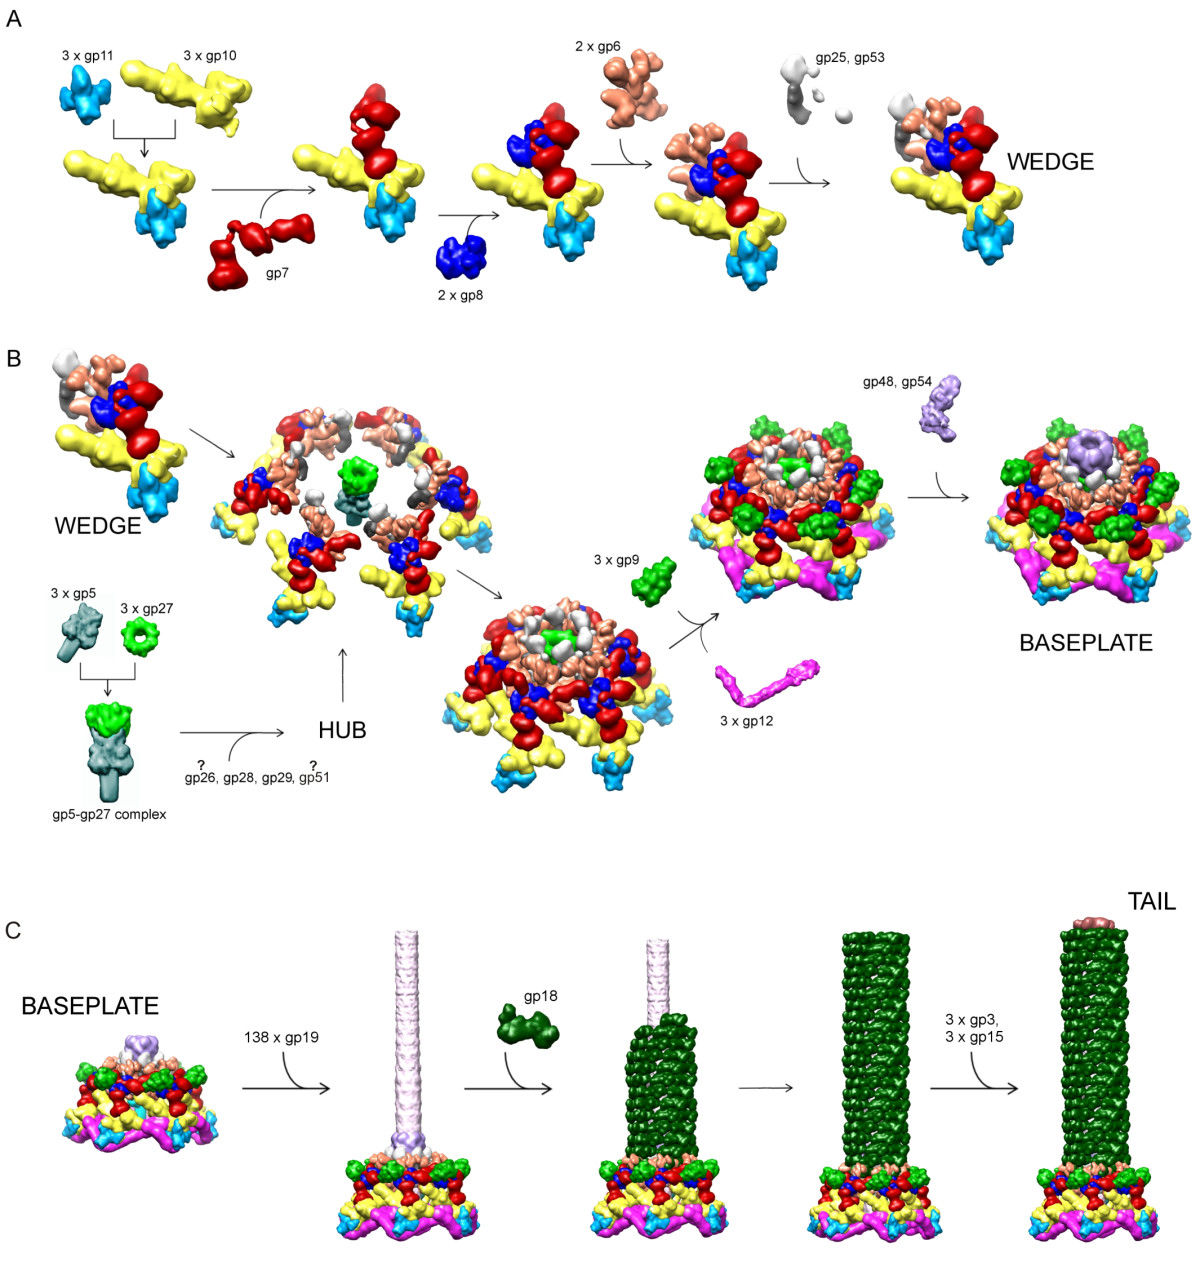
\includegraphics[width=\textwidth, trim={7 230 20 10}, clip]{/Users/joehealey/Documents/Warwick/PhD/Thesis/chapters/intro/img/t4assembly.jpg}
        \captionsetup{singlelinecheck=off, justification=centering, font=footnotesize, aboveskip=15pt, belowskip=10pt}
        \caption{}
        \label{wedgeformation}
    \end{subfigure}%

    \begin{subfigure}[h]{\textwidth}
        \centering
        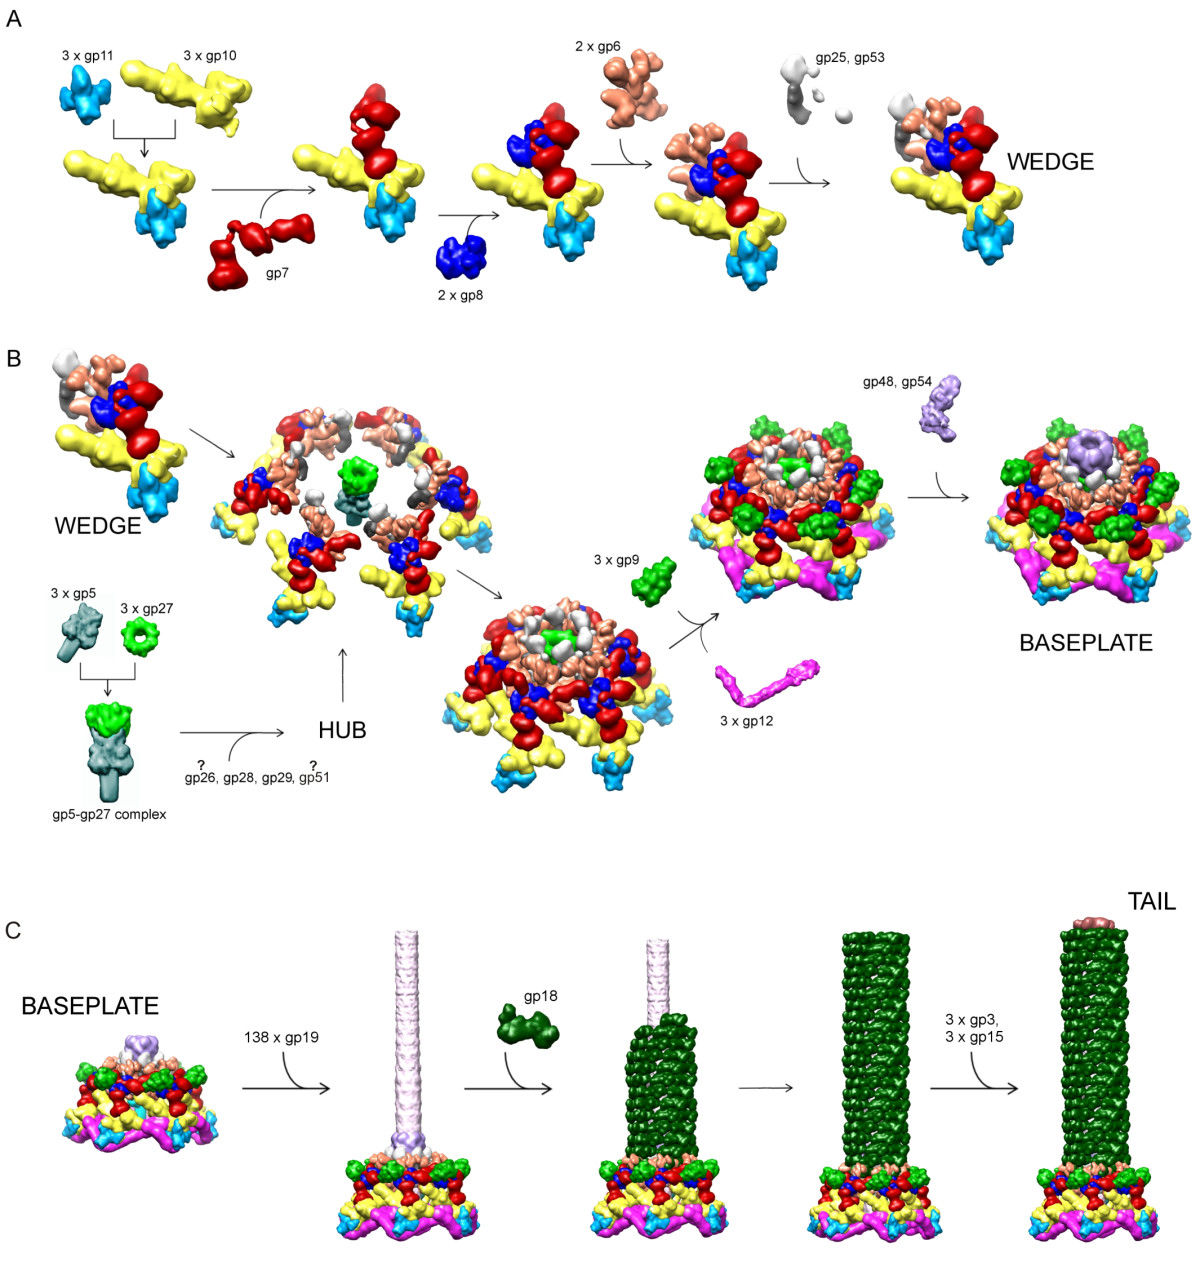
\includegraphics[width=\textwidth, trim={7 105 0 80}, clip]{/Users/joehealey/Documents/Warwick/PhD/Thesis/chapters/intro/img/t4assembly.jpg}
        \captionsetup{singlelinecheck=off, justification=centering, font=footnotesize, aboveskip=15pt, belowskip=10pt}
        \caption{}
        \label{baseplateformation}
    \end{subfigure}%
 
    \begin{subfigure}[h]{\textwidth}
        \centering
        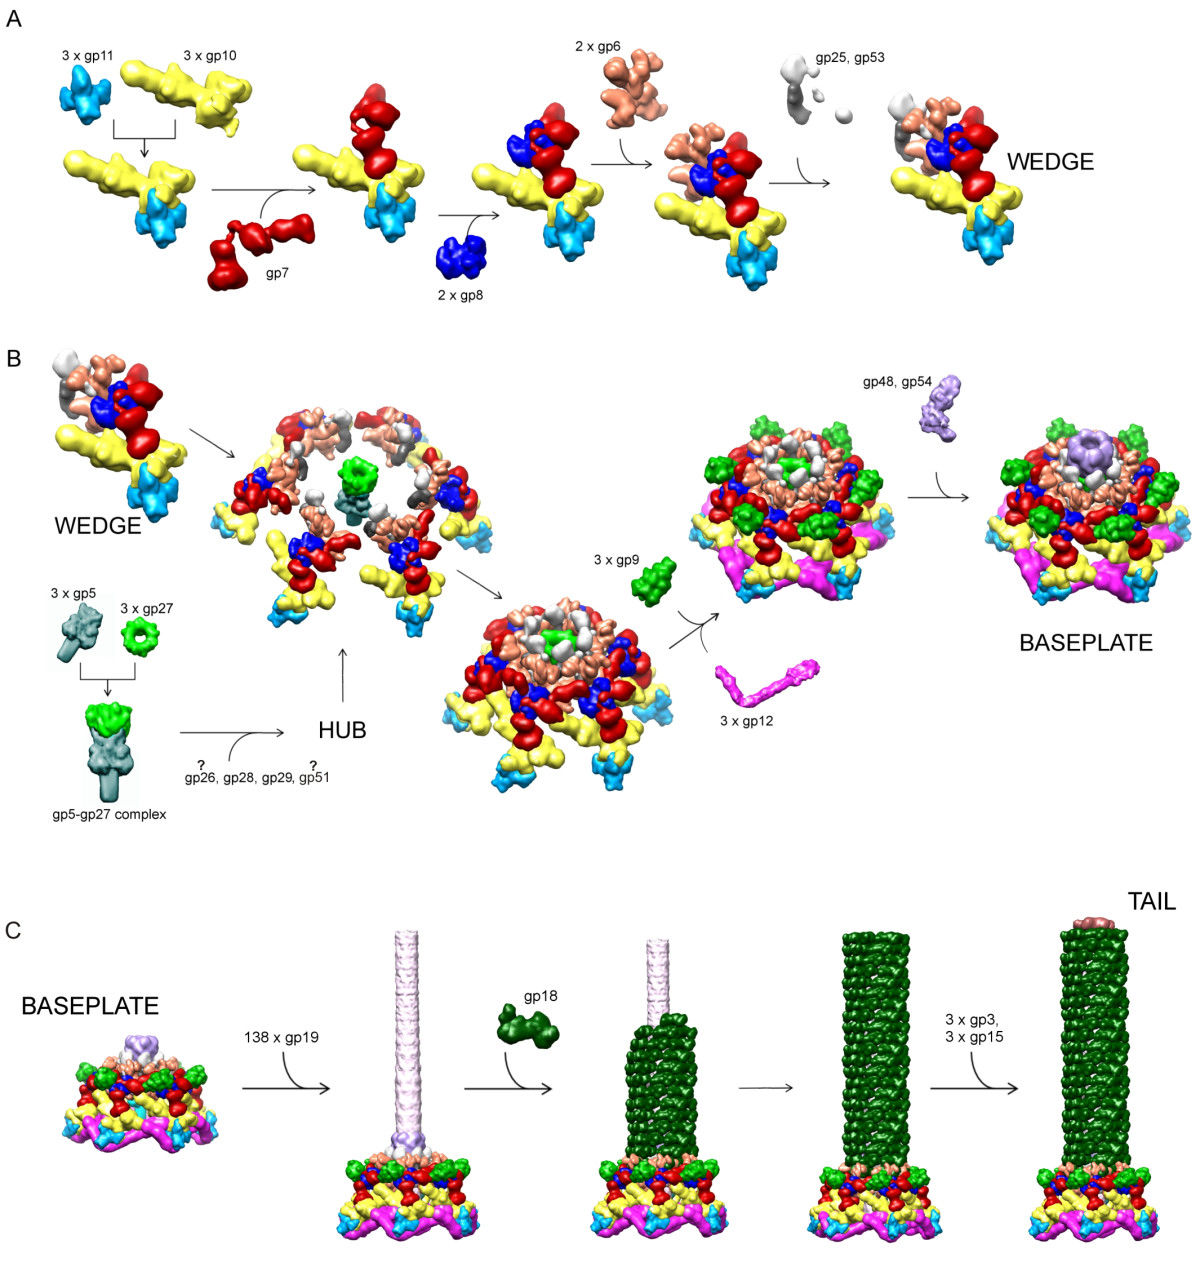
\includegraphics[width=\textwidth, trim={5.5 0 0 210}, clip]{/Users/joehealey/Documents/Warwick/PhD/Thesis/chapters/intro/img/t4assembly.jpg}
        \captionsetup{singlelinecheck=off, justification=centering, font=footnotesize, aboveskip=15pt, belowskip=10pt}
        \caption{}
        \label{tubeformation}
    \end{subfigure}%

	\captionsetup{singlelinecheck=off, justification=justified, font=footnotesize, aboveskip=10pt}
	\caption[Assembly of the T4 phage tube and baseplate]{\textsc{\normalsize The structural components of T4 and their stoichiometric assembly.} \vspace{0.1cm} \newline \textbf{(A)} The formation of the  ``baseplate wedge" subunit, which is, itself comprised of 6 different proteins and which makes up the majority of the baseplate. \textbf{(B)} Shows the formation of the complete baseplate, where the spike baseplate hub complex and tail fibres are added. The overall baseplate is made up of 6 wedge complexes which are further complexed together, with the addition of tail fibres and a number of other baseplate proteins including the collar. \textbf{(C)} A depiction of the complex between the baseplate structure and the polymerisation of the tail tube. The collar interfaces with the interior tube, around which almost 150 copies of gp18 are helically polymerised before termination and capping. Adapted and reproduced from \cite{Leiman2004} and \cite{Yap2014a}.}
	\label{t4assemblyflowchart}
\end{figure}
 %%%%%%%%%%%%%%%%%%%%%%%%%%%%%%

\begin{figure}[p]
\thisfloatpagestyle{augment}

\centering
\tabskip=0pt
\valign{#\cr
\hbox{%
    \begin{subfigure}[b]{0.45\textwidth}
        \centering
        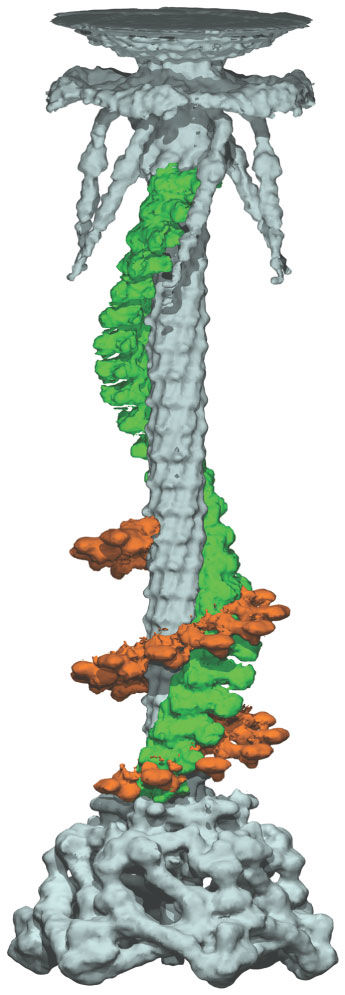
\includegraphics[width=\textwidth, trim={0 0 0 10}, clip]{/Users/joehealey/Documents/Warwick/PhD/Thesis/chapters/intro/img/nsmb975-F5.jpg}
        \captionsetup{singlelinecheck=off, justification=centering, font=footnotesize, aboveskip=10pt}
        \caption{}
        \label{t4sheaths}
    \end{subfigure}%
}\cr
\noalign{\hfill}
\hbox{%
    \begin{subfigure}[t]{0.45\textwidth}
        \centering
        \scalebox{-1}[1]{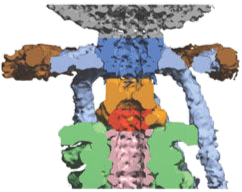
\includegraphics[width=\textwidth, trim={0 0 0 0}, clip]{/Users/joehealey/Documents/Warwick/PhD/Thesis/chapters/intro/img/nsmb975-F2.png}}
        \captionsetup{singlelinecheck=off, justification=centering, font=footnotesize, aboveskip=10pt}
        \caption{}
        \end{subfigure}%
}\vfill
  \hbox{%
    \begin{subfigure}[t]{0.42\textwidth}
        \centering
        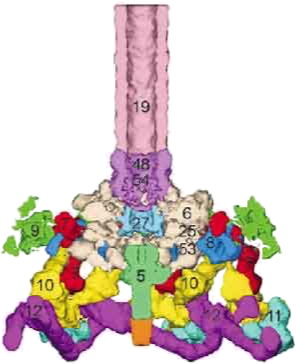
\includegraphics[width=\textwidth, trim={0 0 0 0 }, clip]{/Users/joehealey/Documents/Warwick/PhD/Thesis/chapters/intro/img/nsb970-F1.png}
        \captionsetup{singlelinecheck=off, justification=centering, font=footnotesize, aboveskip=10pt}
        \caption{}
    \end{subfigure}%
}\vfill
    \hbox{%
        \begin{subfigure}[t]{0.45\textwidth}
            \centering
            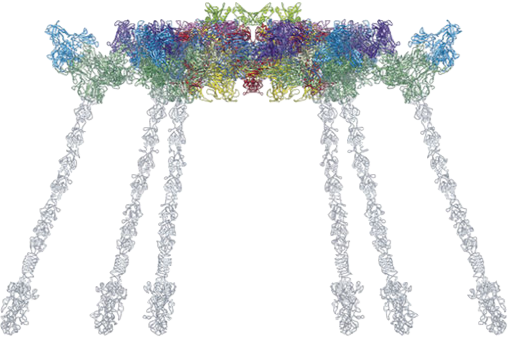
\includegraphics[width=\textwidth, trim={0 0 0 0}, clip]{/Users/joehealey/Documents/Warwick/PhD/Thesis/chapters/intro/img/nature17971-f1.png}
%            \begin{tikzpicture}
%            \node[inner sep=0] (image) {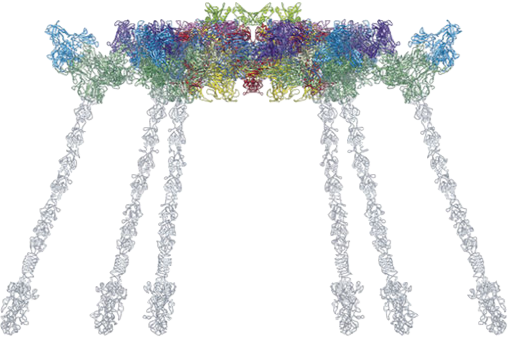
\includegraphics[width=\textwidth, trim={380 480 10 450}, clip]{/Users/joehealey/Documents/Warwick/PhD/Thesis/chapters/intro/img/nature17971-f1.jpg}};
%                    \begin{scope}[x={(image.south east)},y={(image.north west)}]
%                    \draw [fill=white] (10,1) -- (10,3) -- (10,4) -- cycle;
%            \end{scope}
%            \end{tikzpicture}
            \captionsetup{singlelinecheck=off, justification=centering, font=footnotesize, aboveskip=15pt}
            \caption{}
            \label{extendedtailfibres}
        \end{subfigure}%    
  }\cr
}
	\captionsetup{singlelinecheck=off, justification=justified, font=footnotesize, aboveskip=10pt}
	\caption[Resolved T4 Bacteriophage Structures from literature]{\textsc{\normalsize A selection of the resolved structural components of Bacteriophage T4.}\vspace{0.1cm} \newline \textbf{(A)} The T4 EM density reproduced from \cite{Kostyuchenko2005}, the helical outersheath protofilaments are shown in the extended (green) and contracted (orange) conformations. \textbf{(B)} The architecture of the `neck'/`collar' region of the T4 phage, showing the top of the tube. Adapted and  reproduced from Kostyuchenko \emph{et al.} also. \textbf{(C)} The intricate baseplate architecture (shown as a slice-through), adapted and reproduced from \cite{Kostyuchenko2003}. \textbf{(D)} The structure of the lower baseplate complex, showing the extended short tail fibres (they are `retracted' in \textbf{A} and \textbf{C}) adapted from \cite{Taylor2016}. The structure of the genome-containing capsid has been omitted, as the similarity to the tail and baseplate is more relevant. Augmented reality structures coloured according to cylinder radius (red ($\leq$100\AA) to blue ($\leq$20\AA). }
	\label{t4structure}
\end{figure}

\clearpage

\subsubsection{Of PVCs and R-type Pyocins/Tailocins}
The R-type pyocins, particularly those of \emph{Pseudomonas aeruginosa}, have been among the longest studied caudate structures, if Myophages such as those just discussed are discounted, with papers describing their structure and activity as far back as 1965 \citep{Ishii1965}, and they were discovered as early as 1954 \citep{jacob1954biosynthese}. Nevertheless, it took until 2015 for the structure of one of these tailocin structures to be resolved fully \citep{Ge2015} (see \vref{pyocinstructure}). A rapidly growing body of data on the specificity, activity and structure of these types of macromolecular complexes is appearing. `Tailocins' have attracted much attention recently due to their potential use as an alternative to phage therapy. The prospect of utilising bacteriophages has made the public and some of the scientific community understandably nervous, due to their uncontrolled, rapid replication within bacteria, and the introduction of foreign DNA in to the body's microbiome. Tailocins have alleviated some of these concerns due to their highly specific bactericidal activity, similar to phage, but without containing any nucleic material and thus no replicative capacity, and they appear tractable for engineering \citep{Scholl2008}.

Tailocins are so called as they are comprised of bacteriophage tail tube, baseplate and fibre structures, without a capsid or head \citep{Ishii1965}. Bacteria have co-opted these structures in to their genomes such that they can be used as highly specific antimicrobials against other, potentially closely related bacteria, providing considerably higher selective toxicity than is attainable through small molecule antimicrobials \citep{Heo2007}. This section specifically focuses on the ``R-Type" pyocins, which are considered a subclass of bacteriocins (protein or peptide toxic molecules effective against other bacteria; colicins are another well known example). They take their name from the fact that they are `Rod'-like phage tails, being demarcated from the F (`flexious') and S (soluble) type bacteriocins. They derive the name `pyocin' from their discovery in \emph{P. aeruginosa}, as mentioned, as it was renamed from \emph{Pseudomonas pyocynia}. The F-type pyocins are also phage tail like structures, but the tails are not straight tail rods, instead being somewhat curved, and crucially, they are noncontractile, meaning they are more closely related to P2 and $\lambda$ phages, than T-even \emph{Caudoviriales} \citep{Michel-Briand2002,Nakayama2000}. The S-type bacteriocins are small, soluble antimicrobials, more reminiscent of small molecule compounds, and cannot be sedimented or visualised by EM, unlike the F and R types \citep{Heo2007, kageyama1975bacteriocins}. As with the previous section on T4, \vref{pyocinems} shows a selection of R-type pyocin molecules as observed via EM. Hopefully the reader can already appreciate the similarities between the PVCs as shown in \vref{PVCems} and the pyocins in the figures below.


\vspace{0.2cm}
\begin{figure}[h]
\centering
    \begin{subfigure}[b]{0.4\textwidth}
        \centering
        {%
\setlength{\fboxsep}{0pt}%
\setlength{\fboxrule}{1pt}%
        \fbox{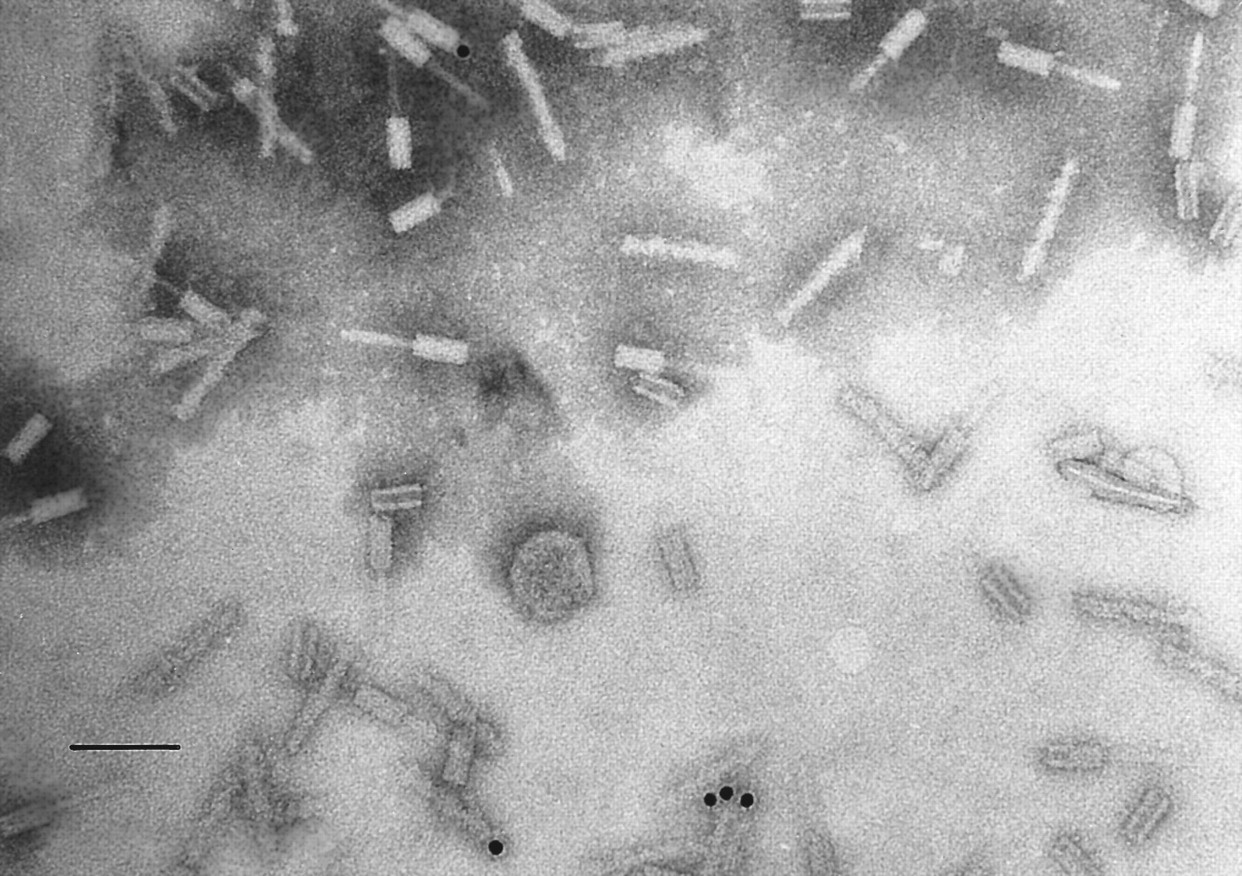
\includegraphics[width=\textwidth, trim={0 98 0 0}, clip]{/Users/joehealey/Documents/Warwick/PhD/Thesis/chapters/intro/img/pyocin.jpg}}
            }%
    \end{subfigure}%
        \begin{subfigure}[t]{0.18\textwidth}
        \centering
        {%
\setlength{\fboxsep}{0pt}%
\setlength{\fboxrule}{1pt}%
        \fbox{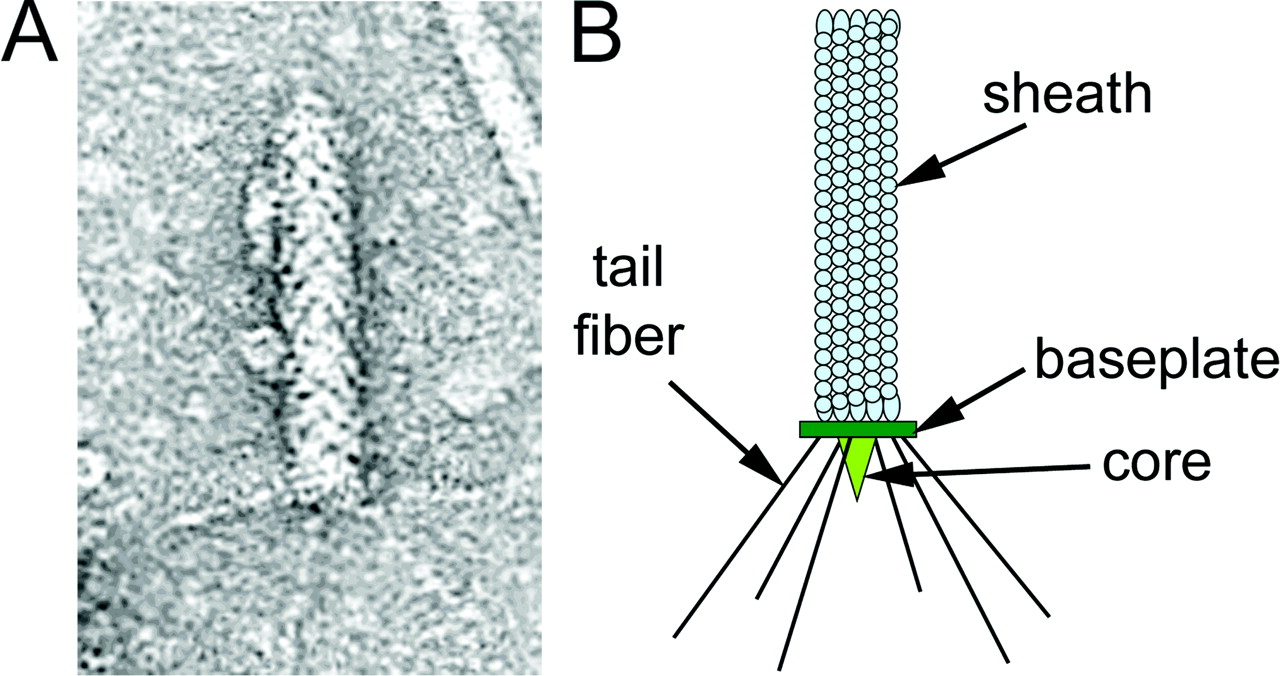
\includegraphics[width=\textwidth, trim={79 10 760 51}, clip]{/Users/joehealey/Documents/Warwick/PhD/Thesis/chapters/intro/img/afplarge.jpg}}
        }%
    \end{subfigure}%
    \begin{subfigure}[t]{0.4\textwidth}
        \centering
        {%
\setlength{\fboxsep}{0pt}%
\setlength{\fboxrule}{1pt}%
        \fbox{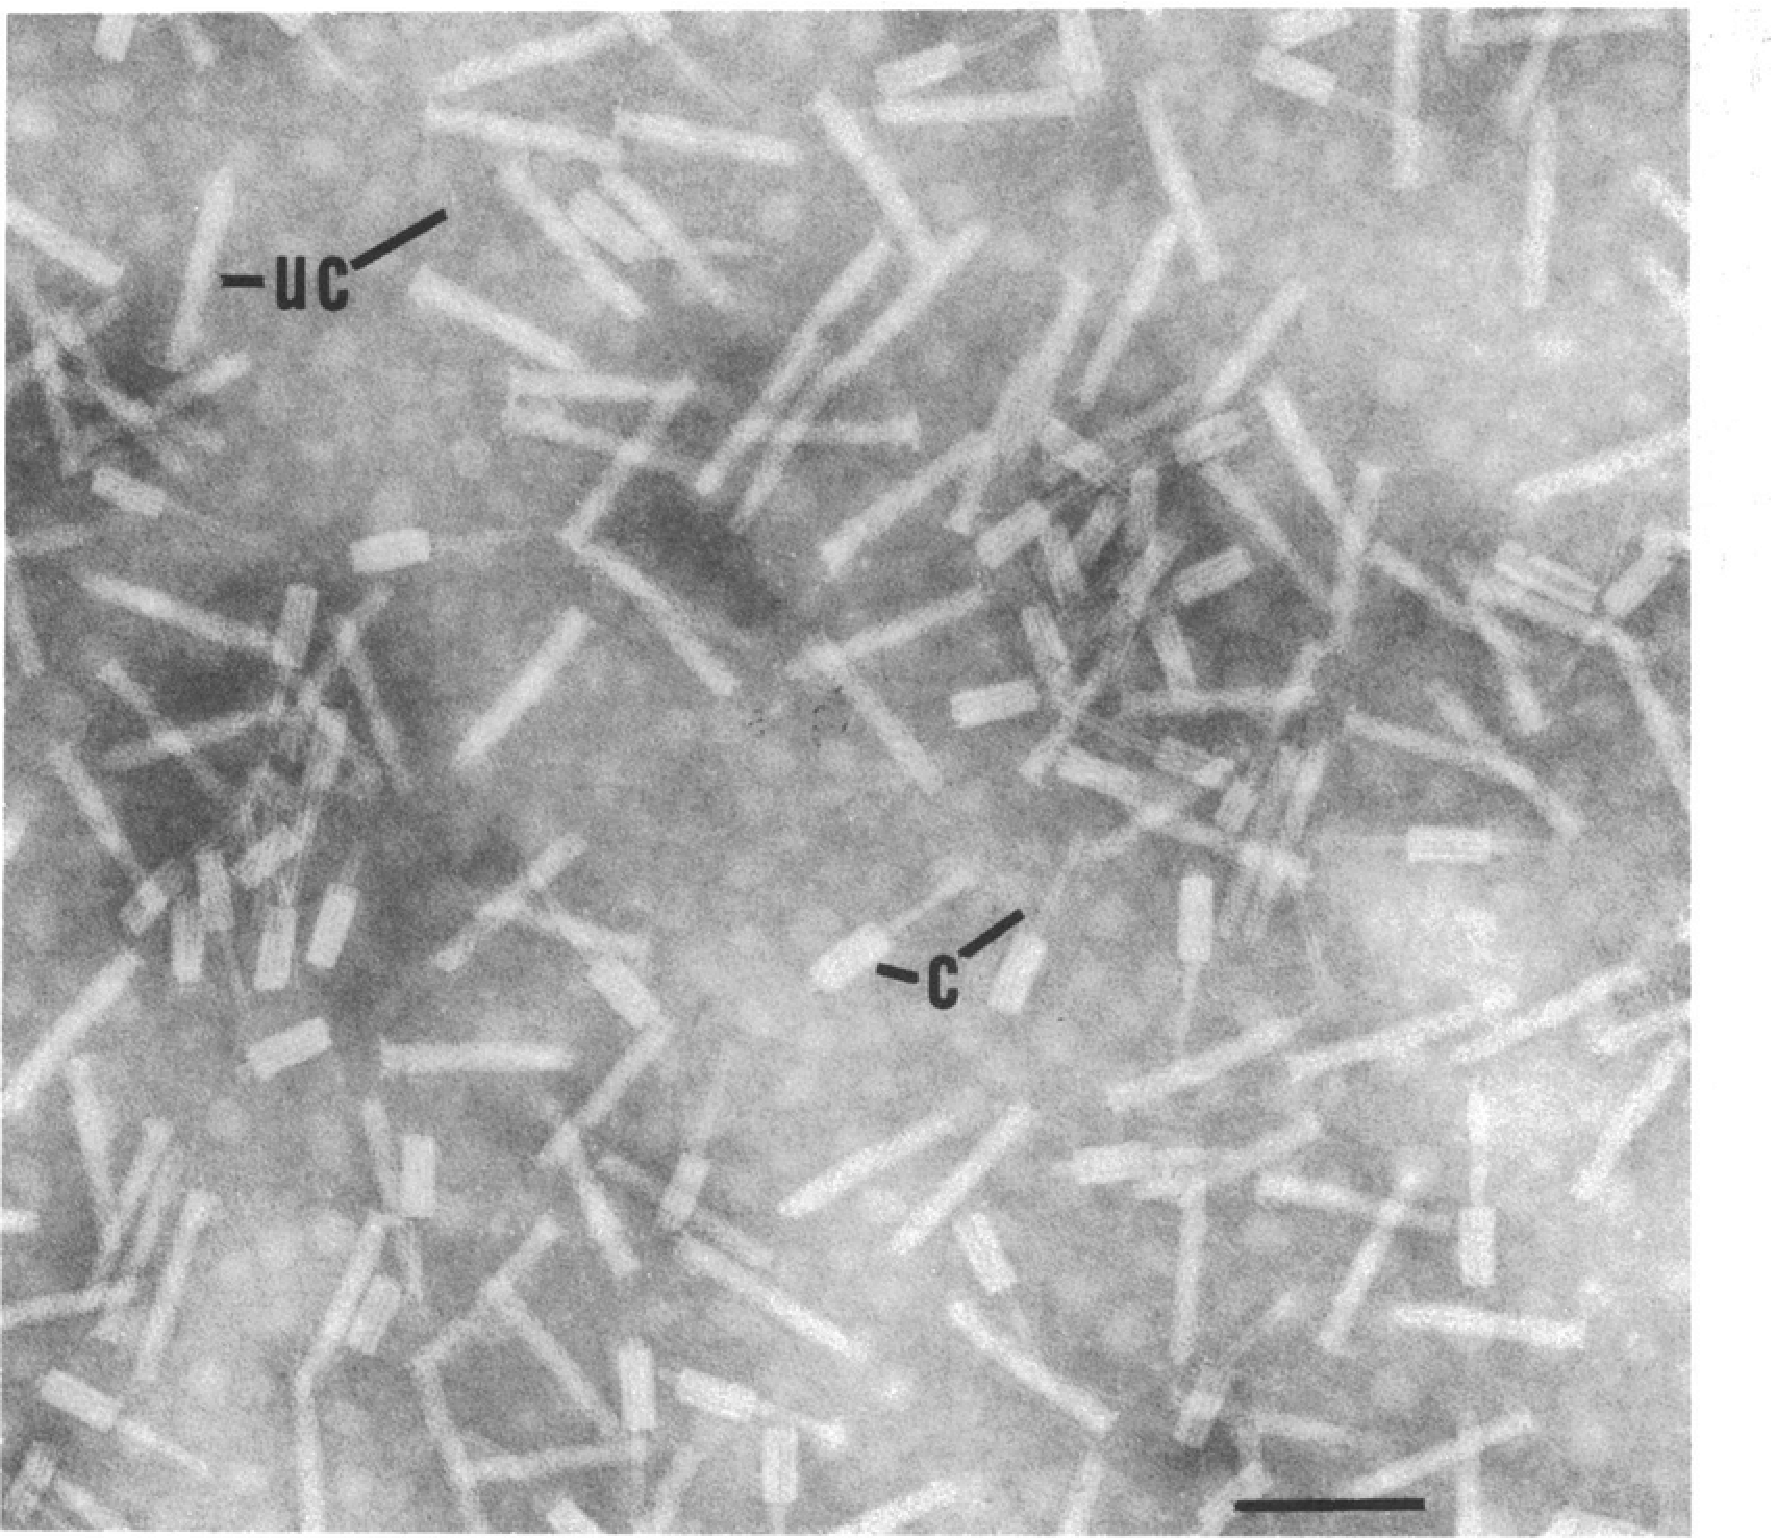
\includegraphics[width=\textwidth, trim={5 200 60 46}, clip]{/Users/joehealey/Documents/Warwick/PhD/Thesis/chapters/intro/img/em_labelled.pdf}}
        }%
        \end{subfigure}%
	\captionsetup{singlelinecheck=off, justification=justified, font=footnotesize, aboveskip=10pt}
	\caption[Electron micrographs of \emph{Pseudomonas} R-type pyocins]{\textsc{\normalsize Electron Micrographs of \emph{Pseudomonas} R-type pyocin particles}\vspace{0.1cm} \newline The left panel shows a number of R-type pyocin molecules purified. The contracted nature of several of the particles reveals clearly the size difference between the inner and outer sheaths. Reproduced from \cite{Lee1999}. The central panel shows a close up image of an individual pyocin particle, where the caudate structure and presence of at least 4 tail fibres is apparent (reproduced from \cite{Williams2008a}. The right hand panel shows R-type pyocin particles in a semi-purified form. The annotations on the image from the original document denote \textbf{UC} - uncontracted particles, and \textbf{C} - contracted particles. Reproduced from \cite{Morse1976}.}
	\label{pyocinems}
\end{figure}


R-type pyocins exert their antimicrobial activity in a similar fashion to bacteriophages, by first using their tail fibre proteins to bind with the lipopolysaccharides (LPS) of other Gram negative bacterial cells of closely related strains. The binding occurs strongly, which provides the necessary anchorage for the next step of toxicity - puncturing. The contractile system, as in the Myophages, drills the tail tube and spike in to the surface of the cell, creating a pore. Unlike the Myophages however, the pyocins contain no translocated material (DNA nor protein) and instead, simply cause a rapid and lethal depolarisation of the bacterial membrane \citep{Uratani1984}. The consensus, at least, is that no material is translocated, though some papers have shown single stranded nucleotide cargoes \citep{Lee1999} - this may be an exception, rather than the rule though. Such is the efficacy and potency of this mechanism of killing, that the pyocins demonstrate `single hit kinetics', meaning a single pyocin complex is sufficient to kill an individual cell \citep{OHKAWA1973}. Roughly 100-200 pyocins can be produced from a single host bacterium, with the first active complexes matured after as little as 45 minutes after induction \citep{Michel-Briand2002, Shinomiya1972, Scholl2008}.

The R-type pyocins structurally resemble something of a `halfway house' between phage and PVC-like systems; they have `streamlined' genetics, by way of removal of the capsid genes and the associated replicative machinery, though the evolutionary relationships between them remain unknown. The pyocins are also a good example of the ubiquity of contractile tail systems in nature, underscoring their potentially pivotal role in the shaping of ecosystems, being elaborated by around 90\% of \emph{Pseudomonas} strains \citep{Michel-Briand2002}, being widespread amongst Gram negatives (particularly among other \emph{Enterobacteriaceae}) \citep{Coetzee1968} and examples also being found in Gram positives such as \emph{Listeria} \citep{Zink1995} and \emph{Staphylococcus} \citep{Birmingham1981, Scholl2008}. 

Even with this seeming ubiquity among various clades within bacteria, it's interesting to observe and speculate at this point, on the possible link between these microbial `weapons' and their abundance in species of bacteria which are thought to have some marine origins. \emph{Pseudomonas} is known to be associated with marine and generally aquatic environments, and this has been a long running hypothesis for the origins of \emph{Photorhabdus} itself (two `smoking guns' for this being that it has retained the \emph{lux} operon, which is otherwise exclusive to marine organisms, and its frequent isolation near coastlines). It seems that the ability to produce a caudate structure which can be deployed at a distance could have some extra utility in aquatic environments - and some further examples of innovative tailocin like structures are discussed in Section 1.2.3.5.1 on page 47 and Section 1.2.3.5.1 on page 48. \cite{Persson2009} have also made a similar observation, when they studied the prevalence of various pathogenicity islands in marine organisms from the Global Ocean Sampling dataset, including islands like the Antifeeding prophage (see \vref{afp}).

The seminal paper which finally resolved the intricacies of the the structure of the R-type pyocins was that of \cite{Ge2015}. Not only were they able to obtain high resolution EM maps of the structure, they managed to resolve, atomistically, both the pre- and post-contraction states. \vref{pyocinstructure} reproduces this data.


\begin{figure}[p]
\thisfloatpagestyle{augment}
\centering
\tabskip=0pt
\valign{#\cr
\hbox{%
    \begin{subfigure}[b]{0.3\textwidth}
        \centering
        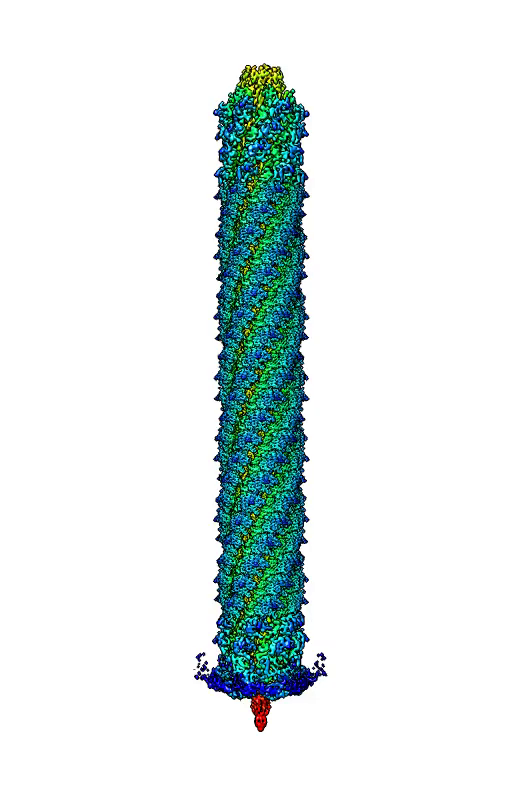
\includegraphics[width=\textwidth, trim={170 40 180 60}, clip]{/Users/joehealey/Documents/Warwick/PhD/Thesis/chapters/intro/img/videostill.png}
        \captionsetup{singlelinecheck=off, justification=centering, font=footnotesize, aboveskip=10pt}
        \caption{}
        \label{videostill}
    \end{subfigure}%
}\cr
\noalign{\hfill}%\vspace{1cm}
\hbox{%
    \begin{subfigure}[t]{0.65\textwidth}
        \centering
        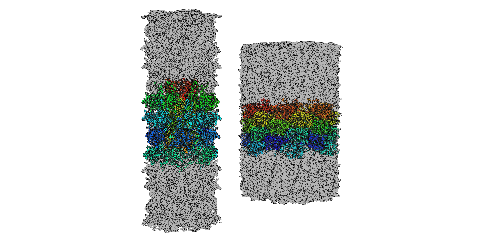
\includegraphics[width=\textwidth, trim={65 2 65 2}, clip]{/Users/joehealey/Documents/Warwick/PhD/Thesis/chapters/intro/img/pyocin_maps.pdf}
        \captionsetup{singlelinecheck=off, justification=centering, font=footnotesize, aboveskip=10pt}
        \caption{}
        \end{subfigure}%
}\vfill
    \hbox{%
        \begin{subfigure}[t]{0.68\textwidth}
            \centering
            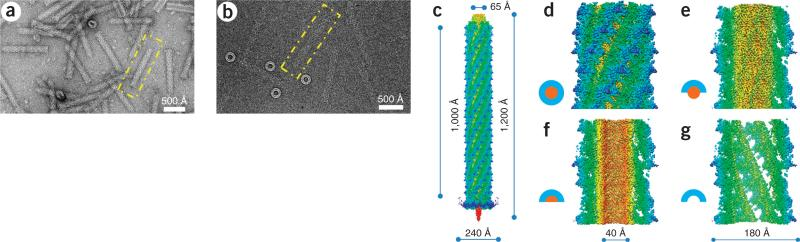
\includegraphics[width=\textwidth, trim={200 0 0 0}, clip]{/Users/joehealey/Documents/Warwick/PhD/Thesis/chapters/intro/img/pyocintube.jpg}
            \put(-91,168){\obscure{0.5cm}{0.5cm}}
            \put(-91,76){\obscure{0.5cm}{0.5cm}}
            \put(-195,168){\obscure{0.5cm}{0.5cm}}
            \put(-195,77){\obscure{0.5cm}{0.5cm}}
            \put(-279,167){\obscure{0.5cm}{0.5cm}}
            \captionsetup{singlelinecheck=off, justification=centering, font=footnotesize, aboveskip=15pt}
            \caption{}
            \label{slicedtube}
        \end{subfigure}%    
  }\cr
}
	\captionsetup{singlelinecheck=off, justification=justified, font=footnotesize, aboveskip=10pt}
	\caption[Resolved R-type Pyocin Structures from \cite{Ge2015}]{\textsc{\normalsize The structures of the R-type pyocin from \cite{Ge2015}.}\vspace{0.1cm} \newline \textbf{(A)} The reconstructed pyocin EM density reproduced from the Supplementary Video 1 of the \cite{Ge2015} paper as a snapshot. The structure is coloured according to its distance from the central axis (colder colours are further away from the centre). \textbf{(B)} Shows the extended and contracted sheath structures for the pyocin from EMDB-6270 (extended) and EMDB-6271 (contracted) with the fitted PDBs 3J9Q and 3J9R respectively. These figures were made using the published data, but reproduced independently using UCSF Chimera \citep{Pettersen2004}. \textbf{(C)} Shows sequential cut-aways of the sheaths with \AA{}ngstrom measurements of the inner and outer diameters and lengths. The coloured circles adjacent to each sub-panel are a key to which tube faces have been sliced through (orange = inner, blue = outer).}
	\label{pyocinstructure}
\end{figure}

\clearpage


From \vref{pyocinstructure} the helical nature of the outer sheath is quite apparent. Interestingly though, unlike the T4 phage structure, the inner sheath is not helically offset, instead being a direct stack of hexamers forming the equivalent of the gp19 toroids. The outer sheaths are helically offset relative to one another by 18.3$^{\circ}$, with a right handed spiral, and are translated by 38.4$^{\circ}$ along the vertical helix axis \citep{Ge2015, Kube2015a}. Thus the hexameric helix is, in effect, more `tightly wound', by having a greater deal of twist, and less vertical rise per unit versus the T4 sheath (in the extended configuration). The outer sheath differs further still as it is comprised of much simpler monomers. The molecular weight of the gp18 monomers is $\approx$71.3 kDa, whereas the equivalent outer sheath protein in the R-type pyocin is only 41.2 kDa. This can also be seen from the structures themselves, as the pyocin monomers seem to lack the protrusions that the T4 gp18 protomers have to quite the same degree, though there is still a noticeable ridge-trough-ridge architecture to the tube \citep{Kube2015a}. From the atomic reconstruction, it was shown by Ge and colleagues that each protomer of the outer sheath interacts with the adjacent 2 protomers via extensions of the N and C termini of the individual monomers with the C-terminal reaching out to the monomer to the right, and the N-terminal to the left. Thus the outer sheath of the R-type pyocin actually more closely resembles a mesh, like a chain-link fence, encompassing the inner sheath, but with the ability to transduce a contraction force along its length \citep{Ge2015}. The bottom left panel of \vref{slicedtube} demonstrates this, as the outer sheath cutaway can be seen through completely from the interior. This interaction has also been observed in bacterial pili and Type 6 Secretion Systems, and previously referred to as the ``$\beta$-augmentation mechanism" \citep{Remaut2006}. Mutagenesis studies showed that these interwoven strands were essential for the contractile mechanism in the T6SS, though were not required for assembly, suggesting that hydrostatics are largely responsible (which is also consistent with the spontaneous self assembly of Hcp monomers seen in \cite{Ballister2008}) \citep{Kudryashev2015, Clemens2015}. The Ge et al. paper also made the observation that there is no structural interaction between subunits of the outer sheath beyond the terminal extensions. The primary interactions in the outer sheath are actually along individual helical protofilaments - i.e. one subunit interacts with the subunits above-right, and below-left of it. 

The inner sheaths rings display complementary surface charge, further suggesting that they are self-assembled in a hydrostatically driven manner. In effect, each disk could be considered a bar magnet, with an electrostatic `north and south pole' (really an electrostatic dipole), ensuring they assemble correctly in a head-to-tail fashion \citep{Ge2015}. The inner sheath monomers of the pyocin consists of 2 anti-parallel $\beta$-sheets, which are orthogonal to one another in strand direction by approximately 90$^{\circ}$. It was noted that they form a similar structure to the well known `jelly roll' or `cupin' fold where 2 sets of 4 $\beta$-strands are opposed to one another \citep{Richardson1981, Dunwell2004}, but are actually thought to be unrelated, despite this domain being highly conserved in other viral and (to a lesser degree) cellular protein sequences. The 6 monomers combine to form one of the largest $\beta$-barrel structures to be resolved yet with 24 $\beta$-strands forming the inner circumference of the lumen \citep{Ge2015}.

Ge and colleagues have recapitulated an often seen homology modelling approach for the core lumen of the pyocin, and compared its surface charge, and smooth bore to the orthologues from phage $\lambda$ \citep{Pell2009a}, the T6SS \citep{Jobichen2010}, and phage PS1. They observed that the inner lumen of the R-type pyocins are primarily negatively charged, consistent with its putative role in depolarisation of cells by de-protonating the cell interior. Conversely, the inner sheaths of phage are typically positively charged to assist in the conveyance of negatively charged DNA. As the electrostatic potential of proteins is, of course, extremely variable, according to the amino acid sequence and manner of tertiary fold, the Hcp monomers which comprise the T6SS inner sheath have been shown to be largely neutral overall. This then enables these systems to convey all manner of protein cargoes, without any `selectivity'. \vref{structbioinfo} replicates this process in the context of the PVCs sheath proteins, to take a first look, albeit \emph{in silico} at this stage, at the sheath structures and any potential relation to their cargo.

The inner and outer sheaths interact primarily electrostatically, with a small triangular region of negative charge on the outer sheath (on 2 `attachment' helices that protrude upward) corresponding to a triangular region of positive charge on the inner sheath. This causes the inner sheath that corresponds to a given tier/disk in the outer sheath to be offset upwards by roughly 15 \AA, and thus an outer sheath monomer straddles 2 inner tiers. Ge and colleagues showed that this reversible electrostatic interaction is important, as the outer sheath increases in diameter upon contraction, and detaches itself from the inner sheath, enabling it to protrude beyond the end of the outer sheath in order to execute its function and traverse the membrane of a target cell.

All that remains of the structure, the spike complex, baseplate, and tail fibres, were not well resolved in the Ge et al. study unfortunately. They obtain reasonable densities for the proximal baseplate, being able to identify `spokes' which connect it to the spike, but do not speculate on, nor provide, further detail or its atomistic structure. It is evident from \vref{videostill}, however, that the baseplate is much stripped down versus the T4, mirroring the streamlining that is also seen in the removal of the capsid, long fibres, and replicative machinery, serving purely as a mounting point for the tail fibres seemingly. As with the baseplate, for the spike complex, detail was lost as a result of their averaging process. Fortunately, its density is also easy to identify from \vref{videostill}, and Ge et al report that they were able to locate a co-ordinated metal ion in the tip (typically iron or zinc), which is a hallmark of gp5-gp27 and VgrG-like spike proteins \citep{Shneider2013, Kube2015a, Browning2012}.

In summary, the structure of the R-type pyocins appears to more accurately reflect the simplicity that is seen in the PVC operons, following a streamlining process associated with non-replicative entities. From the studies to date however, pyocins have only ever demonstrated anti-prokaryotic activity, while on the other hand, PVCs have only ever demonstrated anti-eukaryotic activity. Now, while this may be due to not testing each complex against an exhaustive repertoire of prokaryotes and eukaryotic cell types, these specificities seem to fit with what is known of their basic biology. This means that there is still much to be discovered about what makes PVCs different, and allows them to act on various higher order cell types in the few genes that are remaining without fully understood functions.



\subsubsection{Of PVCs and the \emph{Serratia entomophila} ``Antifeeding prophage"}\label{afp}
This brings us to possibly the nearest cousins of the PVCs - the so-called ``Antifeeding Prophages" of \emph{Serratia}. The Afp was, until the advent of the \cite{Ge2015} paper, the best characterised, closest relative, of the PVCs, and much of what was hypothesised about them was based on analogous experiments on the Afps, borne on a plasmid of \emph{Serratia entomophila} \citep{Rybakova1994}. As its name suggests, like \emph{Photorhabdus}, \emph{S. entomophila} is another common insect pathogen, and they have been shown to be quite closely related \citep{Duchaud2003, Sproer1999, Brillard2002b}. \emph{S. entomophila} causes ``Amber Disease" in the New Zealand grass grub \emph{Costelytra giveni} (formerly \emph{Costelytra zealandica} \citep{Coca-Abia2016}) specifically, and has been used for some time now as a biopesticide \citep{Chattopadhyay2012, OpenderKoul2011}. Electron microscopy studies of purified particles revealed similar morphologies to the Pyocins and PVCs:


\vspace{0.1cm}
\begin{figure}[h]
\centering
    \begin{subfigure}[b]{0.41\textwidth}
        \centering
        {%
\setlength{\fboxsep}{0pt}%
\setlength{\fboxrule}{1pt}%
        \fbox{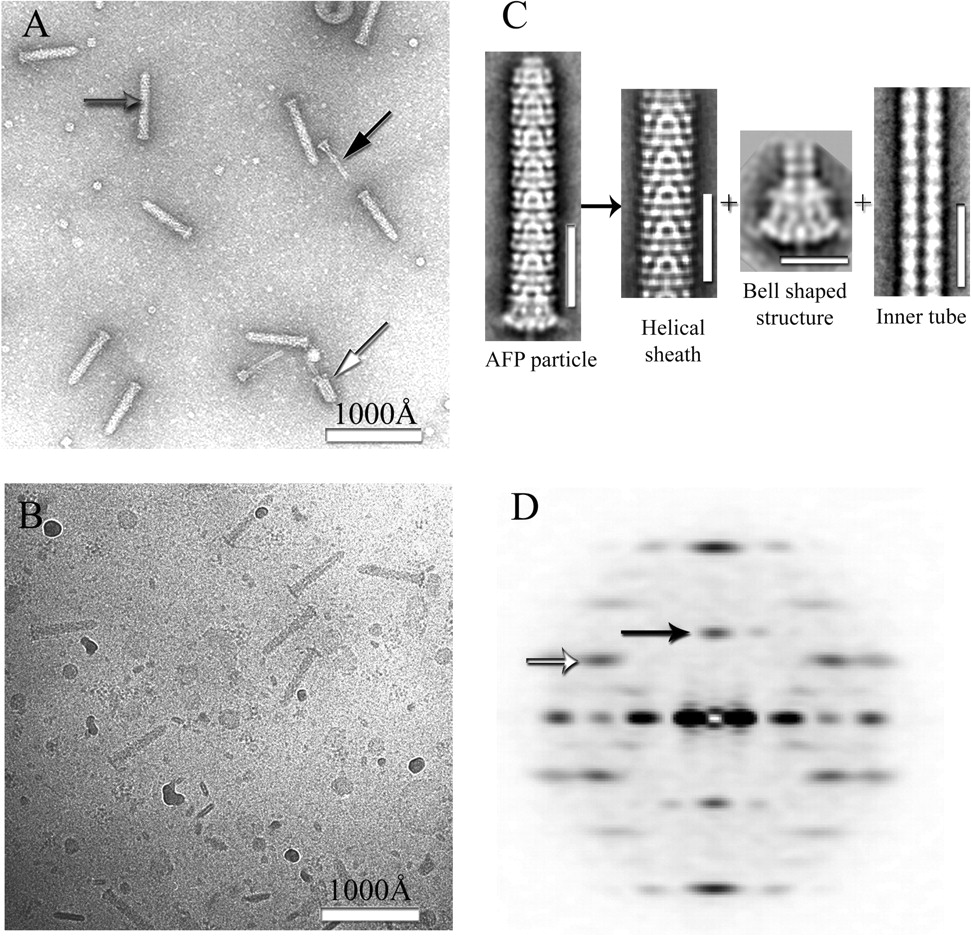
\includegraphics[width=\textwidth, trim={50 700 540 50}, clip]{/Users/joehealey/Documents/Warwick/PhD/Thesis/chapters/intro/img/afp_large.jpg}}
            }%
    \end{subfigure}%
        \begin{subfigure}[t]{0.16\textwidth}
        \centering
        {%
\setlength{\fboxsep}{0pt}%
\setlength{\fboxrule}{1pt}%
        \fbox{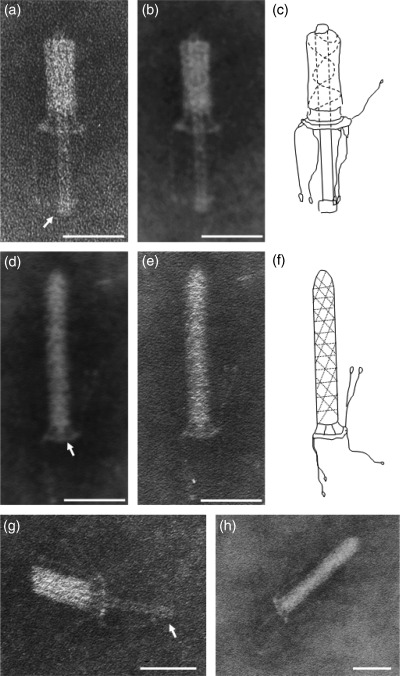
\includegraphics[width=\textwidth, trim={250 5 25 515}, clip]{/Users/joehealey/Documents/Warwick/PhD/Thesis/chapters/intro/img/Afpvariants.png}}
        }%
    \end{subfigure}%
    \begin{subfigure}[t]{0.41\textwidth}
        \centering
        {%
\setlength{\fboxsep}{0pt}%
\setlength{\fboxrule}{1pt}%
        \fbox{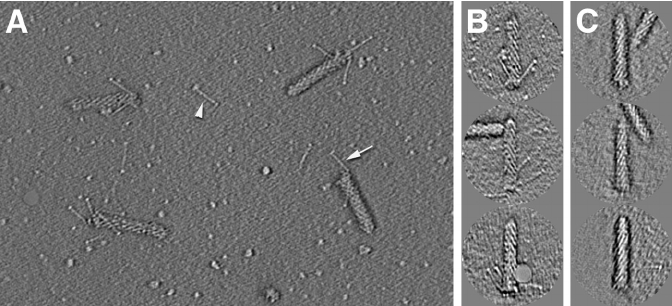
\includegraphics[width=\textwidth, trim={0 45 220 40.2}, clip]{/Users/joehealey/Documents/Warwick/PhD/Thesis/chapters/intro/img/Afp_tomogram.png}}
        }%
        \end{subfigure}%
	\captionsetup{singlelinecheck=off, justification=justified, font=footnotesize, aboveskip=10pt}
	\caption[Electron micrographs of the Antifeeding Prophage]{\textsc{\normalsize Electron Micrographs of the Antifeeding Prophage of \emph{S. entomophila}.}\vspace{0.1cm} \newline The left panel shows EMs of the Afps, revealing their ``bullet like" shape, and similarity to PVCs. The grey arrow denotes a mature, fully intact Afp particle. The black arrow highlights a ``Tube-Baseplate Complex". Adapted and reproduced from \cite{Sen2010}. The centre panel shows a close up of an individual mature Afp, it is just possible to make out the skirt-like formation of the baseplate, and a couple of tail fibres, including one pronate against the tube. Adapted and reproduced from \cite{Hurst2007}. The right hand panel shows more intact Afp particles, and particularly reveals the tail fibre like structures, of which multiple can be seen on any one particle, and some can even be seen loose on the grid (white arrows). Adapted and reproduced from \cite{Heymann2013}.}
	\label{afpEMs}
\end{figure}




The Afps were discovered on the 153,404 bp pADAP (``Amber Disease Associated Plasmid") plasmid \citep{Hurst2011a} due to their pathological effect against \emph{C. giveni}. The plasmid has been shown to contain other virulence factors such as the \emph{sep} toxins (homologues of the well characterised \emph{Photorhabdus} ``Toxin Complex" genes, and thought to be similarly mobile \citep{Dodd2006a}), which are the aetiological agents of ``Amber disease" (and of which \emph{Photorhabdus} also has analogues - in fact, one such \emph{sepC} analogue is a cognate PVC effector) \citep{Hurst2000}. It was observed in the \emph{sep} studies that another large locus on the plasmid caused a cessation of feeding effect 1 to 3 days after ingestion. In later efforts, this was identified as the ``Antifeeding prophage", and hence it earned its name \citep{Hurst2004}. Over almost 10 years, 4 primary papers were published which steadily elucidated the genetic components and pathology \citep{Hurst2004}, the regulation \citep{Hurst2007a} and the structural basis of Afp complexes \citep{Sen2010, Heymann2013}. Additionally, a number of papers were able to identify putative biological roles for some of the more enigmatic proteins in the locus \cite{Rybakova2013, Rybakova2015}. The presence of the Afp on the pADAP replicon was fortunate, as it allowed the whole operon to be subcloned in to lab \emph{E. coli} replicons with relative ease \citep{Hurst2004}. This has allowed quite extensive deletion/mutation studies to be conducted, as well as providing the material for structural resolution. To date, no PVC equivalents have been identified on plasmids in \emph{Photorhabdus}, though in \Plum{} TT01, 4 PVCs appear tandem to one another, surrounded by conjugation machinery and partitioning proteins such as \emph{mukB}, which may be suggestive of an ancestral recombination event between a large plasmid and the chromosome \citep{Yang2006}. More recently, another orthologue of the Afp, termed AfpX has been found in a further strain of \emph{Serratia}, \emph{S. proteamaculans}, once again located on a plasmid, is distinct from the `original' Afp in a number of ways which will be discussed in upcoming sections \citep{Hurst2018}.

The Afp operon is comprised of 18 proteins, termed Afp1-18. Analogues to sheath proteins, spike complexes, baseplate proteins and tail fibre proteins were able to be identified bioinformatically upon first sequencing. A number of proteins were matched to \emph{Photorhabdus} orthologues with unknown functions, revealing the close relationship between these 2 loci, though much of the operon remained poorly understood. Efforts by Rybakova and colleagues were able to shed some light on the roles of Afp14 and Afp16 in the control of tail assembly. In 2013, the function of Afp16 was determined to play a role in the tail length termination process, and stabilised the growing tail tube \citep{Rybakova2013}. Full deletion of this protein resulted in aberrant forms of the Afp, with variable lengths, as well as formation of so-called ``Tube-Baseplate complexes" (TBCs), which lacked much of the outer sheath, but were able to form a truncated inner sheath and seemingly full baseplate arrangement. Trans-expression of Afp16 did not restore a fully matured morphology to the Afps, suggesting that the expression patterns within the operon itself are also key to the self-assembly process, though exogenously applied purified Afp16 to pseudo-denatured Afps did exhibit some restored assembly - though again, not full length. Truncations of the C-terminus of the protein resulted in an intermediate morphology between the TBCs and a fully matured particle. It is still unclear at present how these proteins interact in order to produce the `finished product' however.

In 2015, Rybakova and colleagues were further able to elucidate the role of another enigmatic protein in the formation of the tail tube, this time identifying an analogue of a putative tape measure protein. Truncations of the protein resulted in concomitant shortenings of the elaborated Afp particles, and similarly, elongations of the sequence resulted in particles of increased tail length. Remarkably, there is a near exact linear relationship (R$^2$ = 0.92) between the length of known tail tubes and their associated tape measure proteins \citep{Rybakova2015, Pedulla2003}. Tape measure proteins are difficult to detect via homology alone, as their sequence appears to not be particularly restrictive to function, with no obvious conservation of known phage tape measure domains. The only real hallmarks that have been identified between varied orthologues are a relatively conserved distribution of hydrophobic residues, and atypically high degrees of alpha helical secondary structure. Unusually, the AfpX identified in \emph{S. proteamaculans} has 2 paralogues of the tape measure protein, which vary in length by 36 amino acids. Accordingly, when particles where identified micrographically, a wider distribution of sizes was observed than in the original Afp. The significance of this is not yet understood.

As with the PVCs, at least one of the genes at the 3'-most end of the operon (Afps 17 and 18) are predicted to encode toxic effectors, though unlike the PVCs, there do no not appear to be many variant forms. This is probably one of the reasons that \emph{S. entomophila} maintains a very specific pathogenicity against the grass grub. The Afps, by virtue of their toxic cargoes have been shown to have an LD$_{50}$ of as little as 500 individual Afp particles (though with the potential for multiple toxins to be present per Afp), against an entire insect \citep{Rybakova1994}.
{
\begin{figure}[p]
\thisfloatpagestyle{augment}
\centering
\tabskip=0pt
\valign{#\cr
\hbox{%
    \begin{subfigure}[t]{0.41\textwidth}
        \centering
        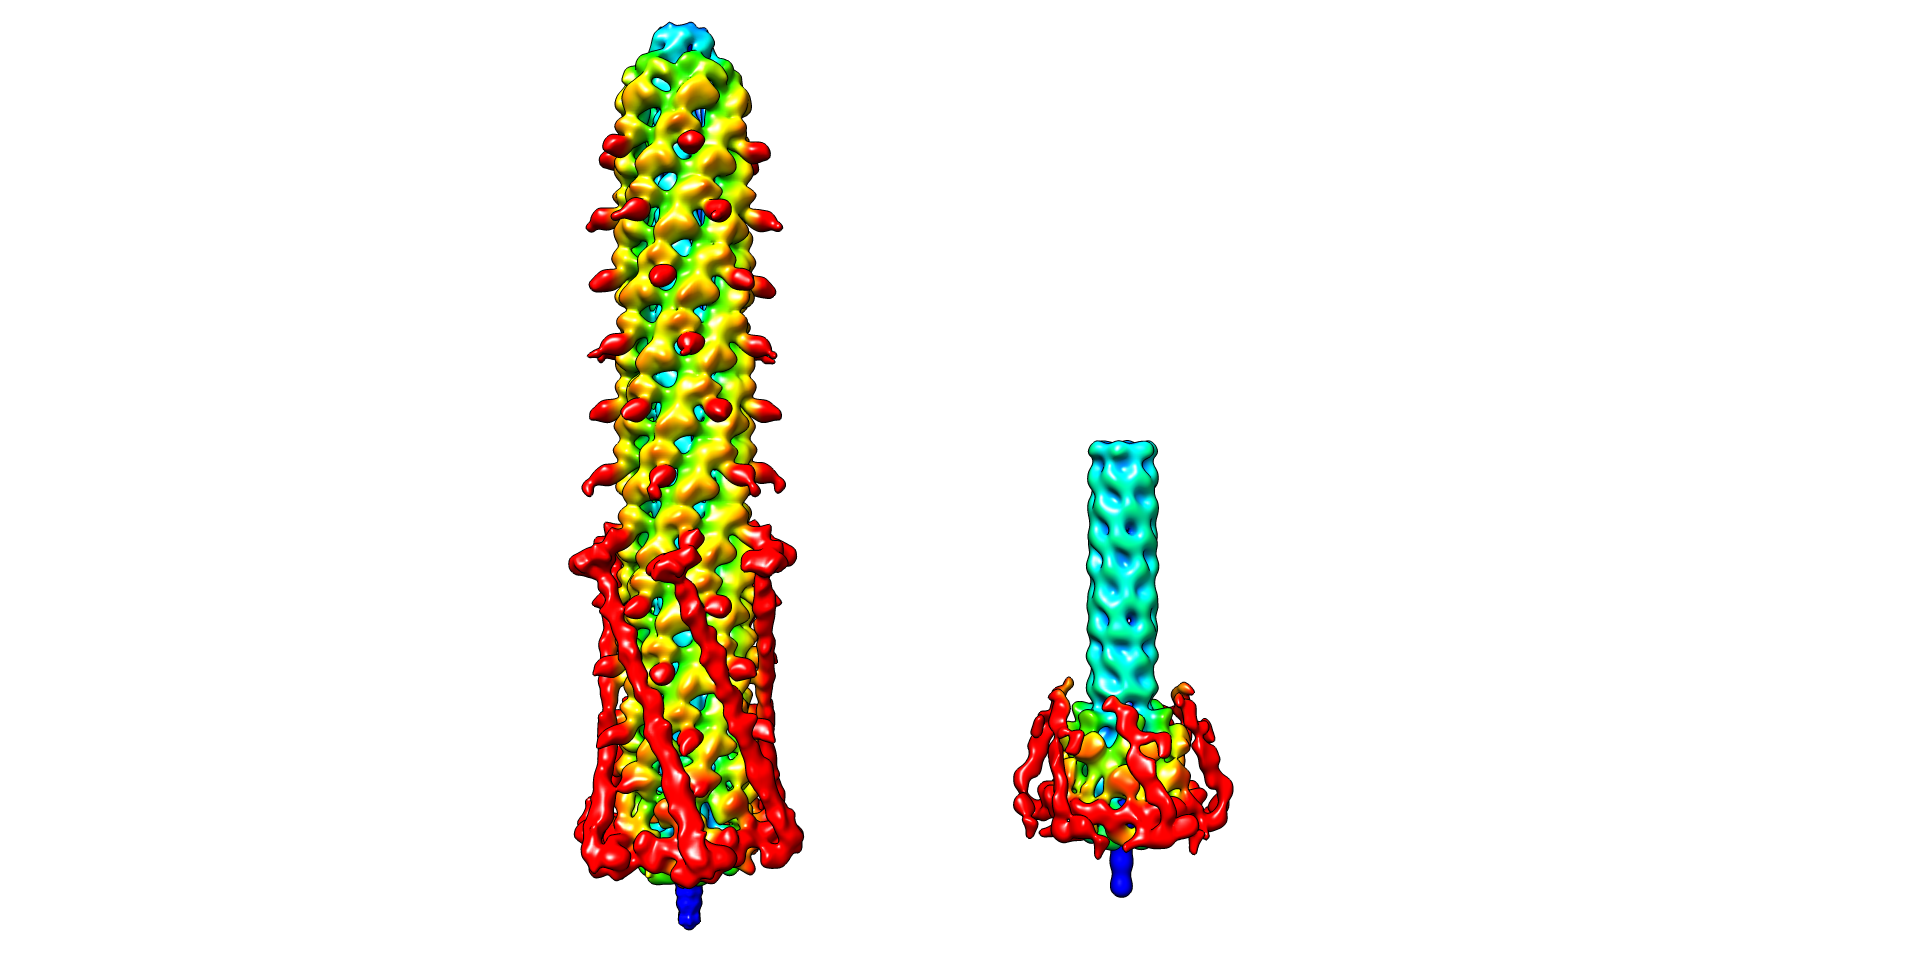
\includegraphics[width=\textwidth, trim={65 3 130 2}, clip]{/Users/joehealey/Documents/Warwick/PhD/Thesis/chapters/intro/img/afp_map_reconstructed.png}
        \captionsetup{singlelinecheck=off, justification=centering, font=footnotesize, aboveskip=10pt}
        \caption{}
        \label{afp1}
    \end{subfigure}%
}\cr
\noalign{\hfill}%\vspace{1cm}
\hbox{%
    \begin{subfigure}{0.58\textwidth}
        \centering
          \begin{tabular}{lr}
            \raisebox{-.5\height}{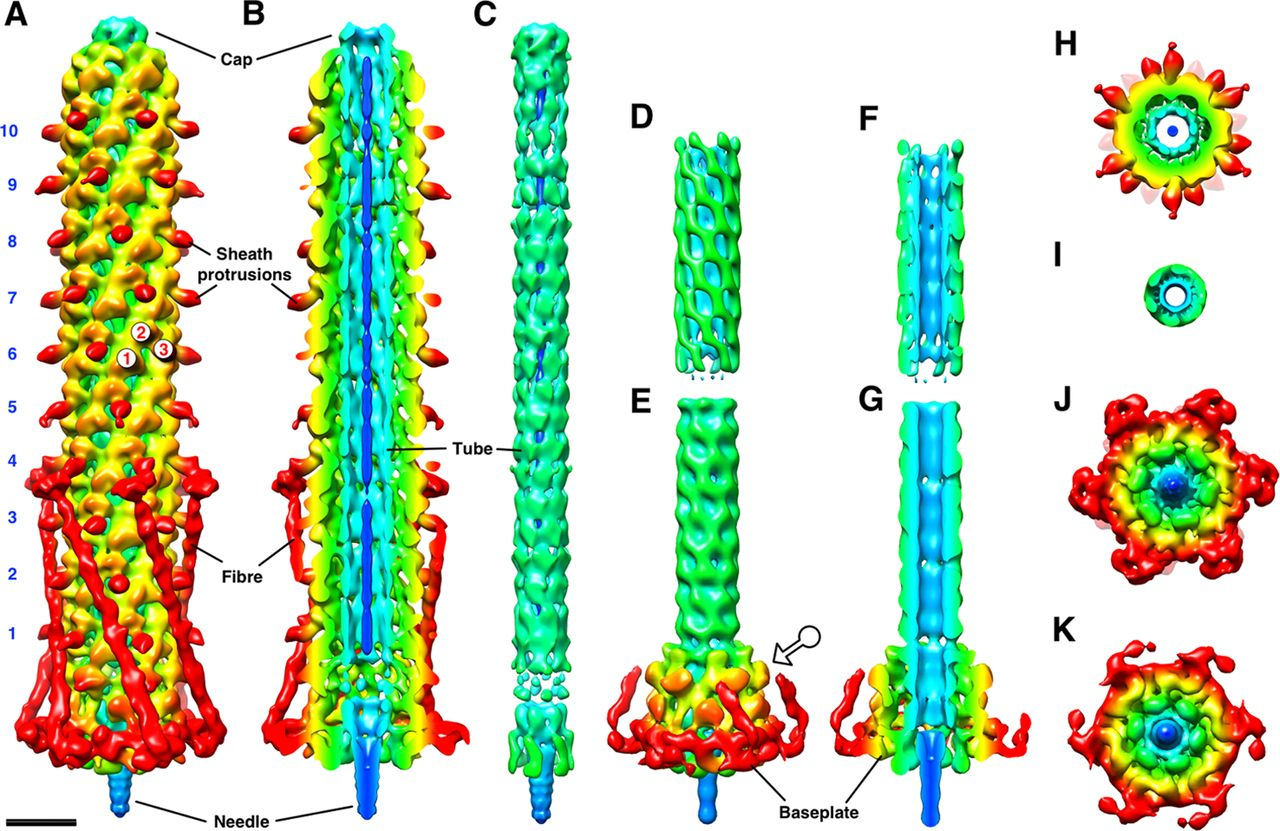
\includegraphics[width=0.49\textwidth, trim={256 143 0 7}, clip]{/Users/joehealey/Documents/Warwick/PhD/Thesis/chapters/intro/img/afp_map.jpg}} &
            \raisebox{-.5\height}{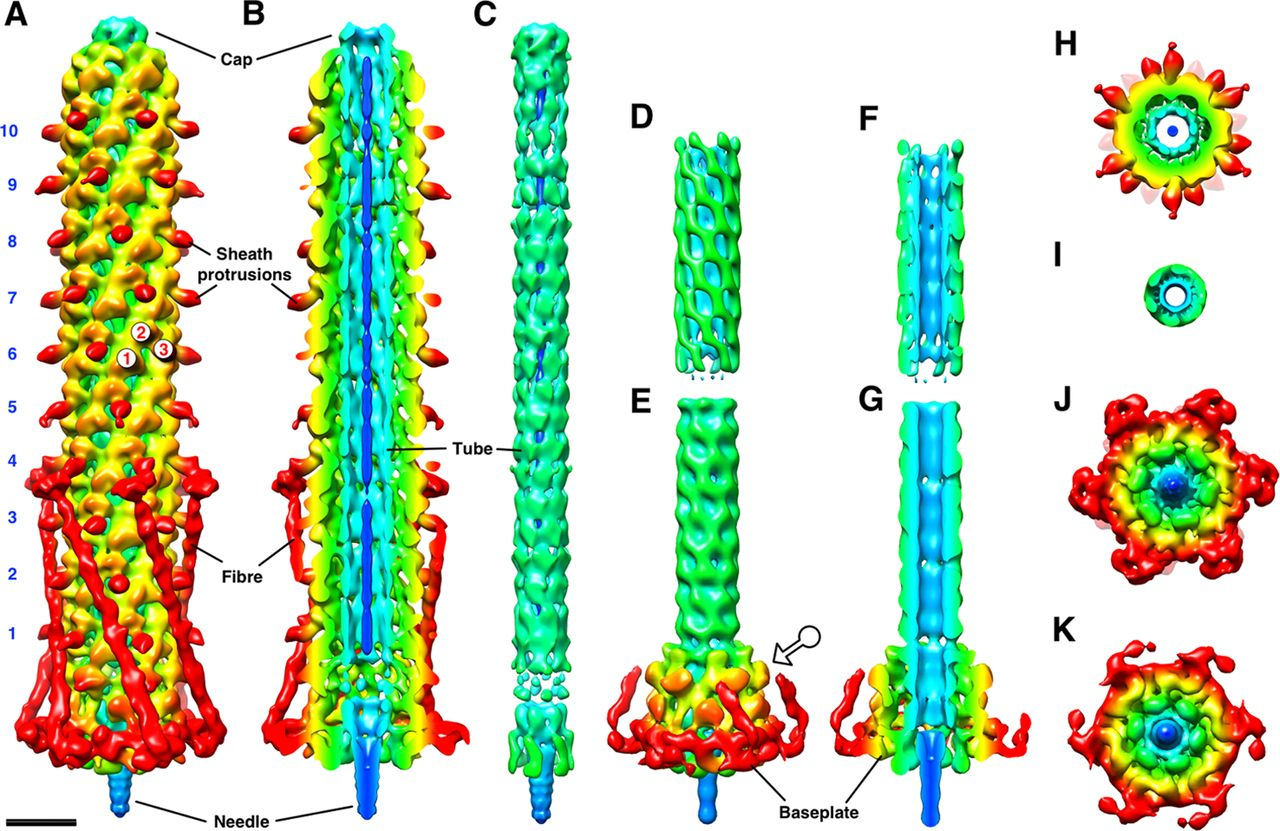
\includegraphics[width=0.49\textwidth, trim={255 55 0 90}, clip]{/Users/joehealey/Documents/Warwick/PhD/Thesis/chapters/intro/img/afp_map.jpg}} \\
                                  
            \raisebox{-.5\height}{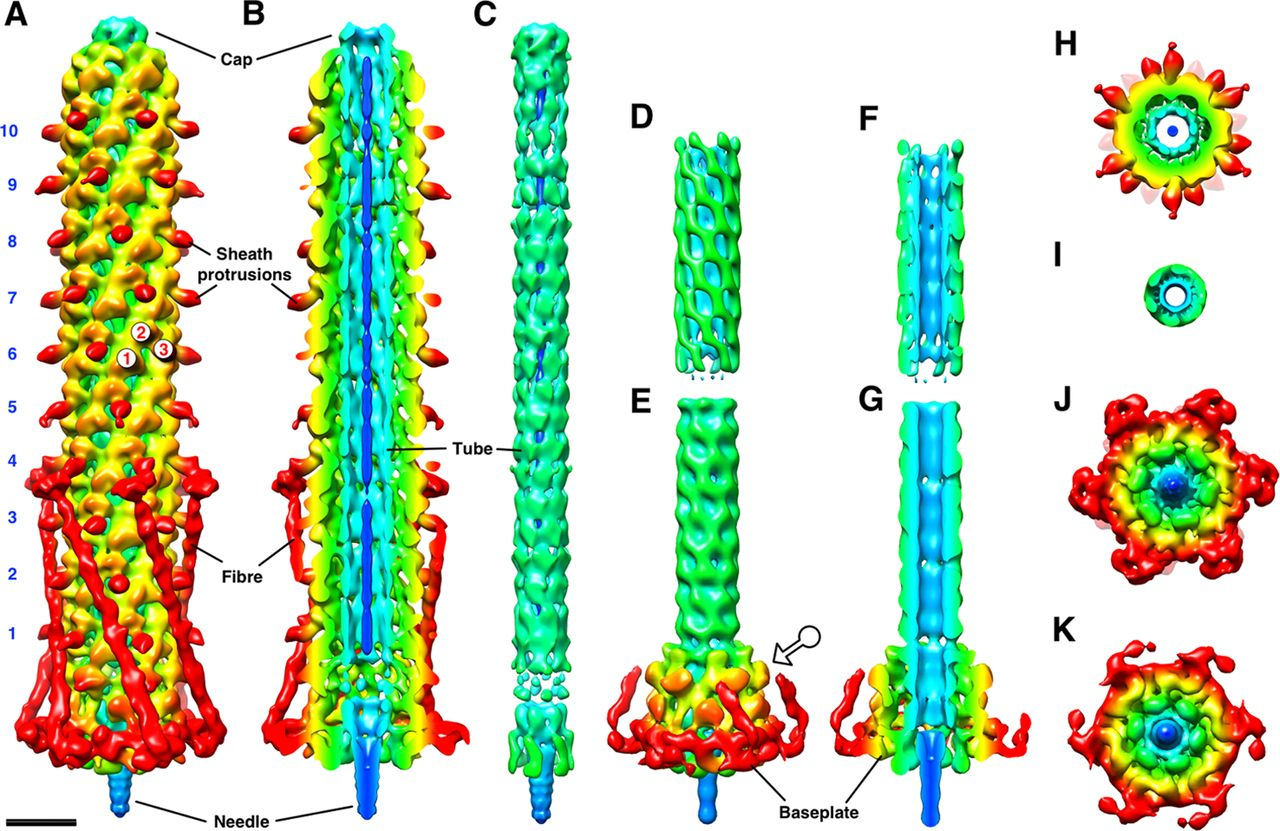
\includegraphics[width=0.49\textwidth, trim={256 120 0 60}, clip]{/Users/joehealey/Documents/Warwick/PhD/Thesis/chapters/intro/img/afp_map.jpg}} &
            \raisebox{-.5\height}{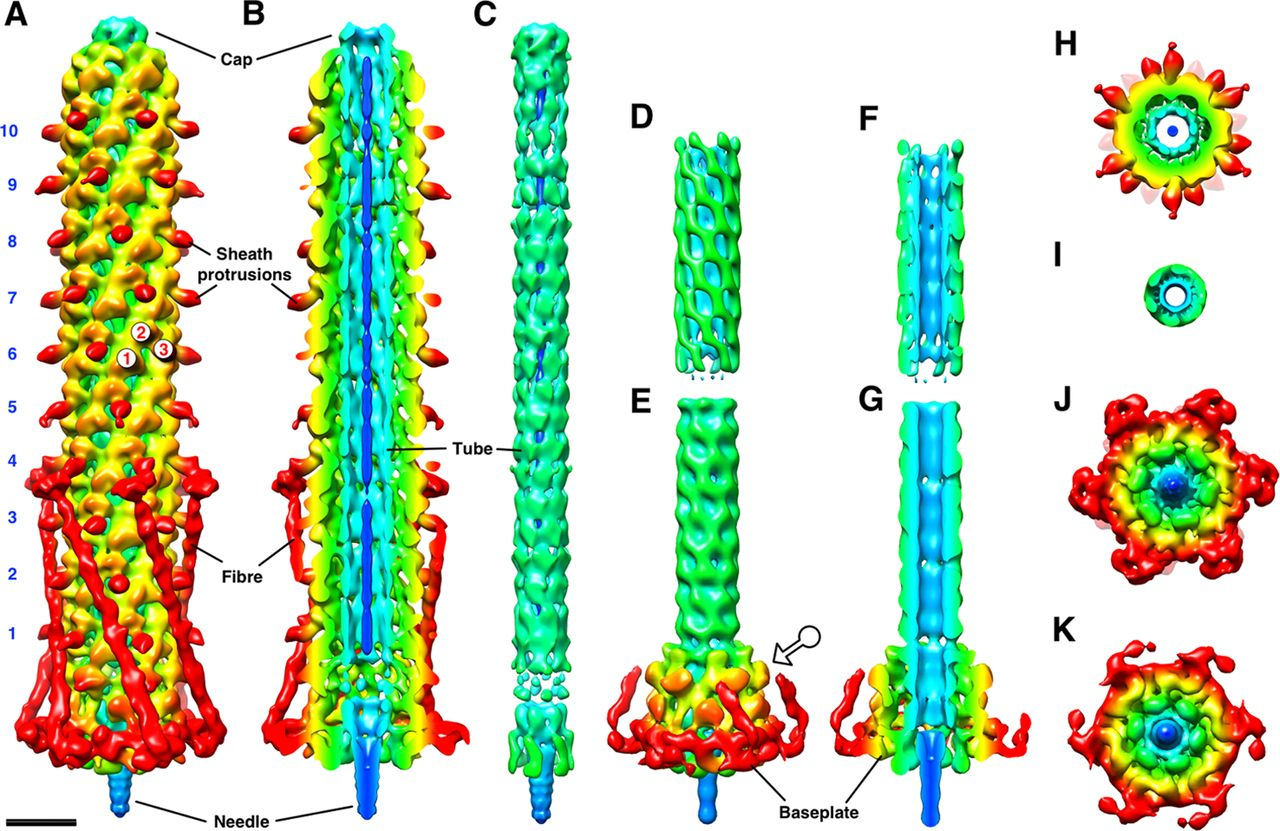
\includegraphics[width=0.49\textwidth, trim={255 0 0 150}, clip]{/Users/joehealey/Documents/Warwick/PhD/Thesis/chapters/intro/img/afp_map.jpg}} \\
     \end{tabular}
            \put(-141,90){\obscure{1cm}{1cm}}
            \put(-265,90){\obscure{1cm}{1cm}}
            \put(-141,-20){\obscure{1cm}{1cm}}
        \captionsetup{singlelinecheck=off, justification=centering, font=footnotesize, aboveskip=10pt}
        \caption{}
        \label{afp2}
        \end{subfigure}%
}\vfill
    \hbox{%
        \begin{subfigure}[t]{0.58\textwidth}
            \centering
            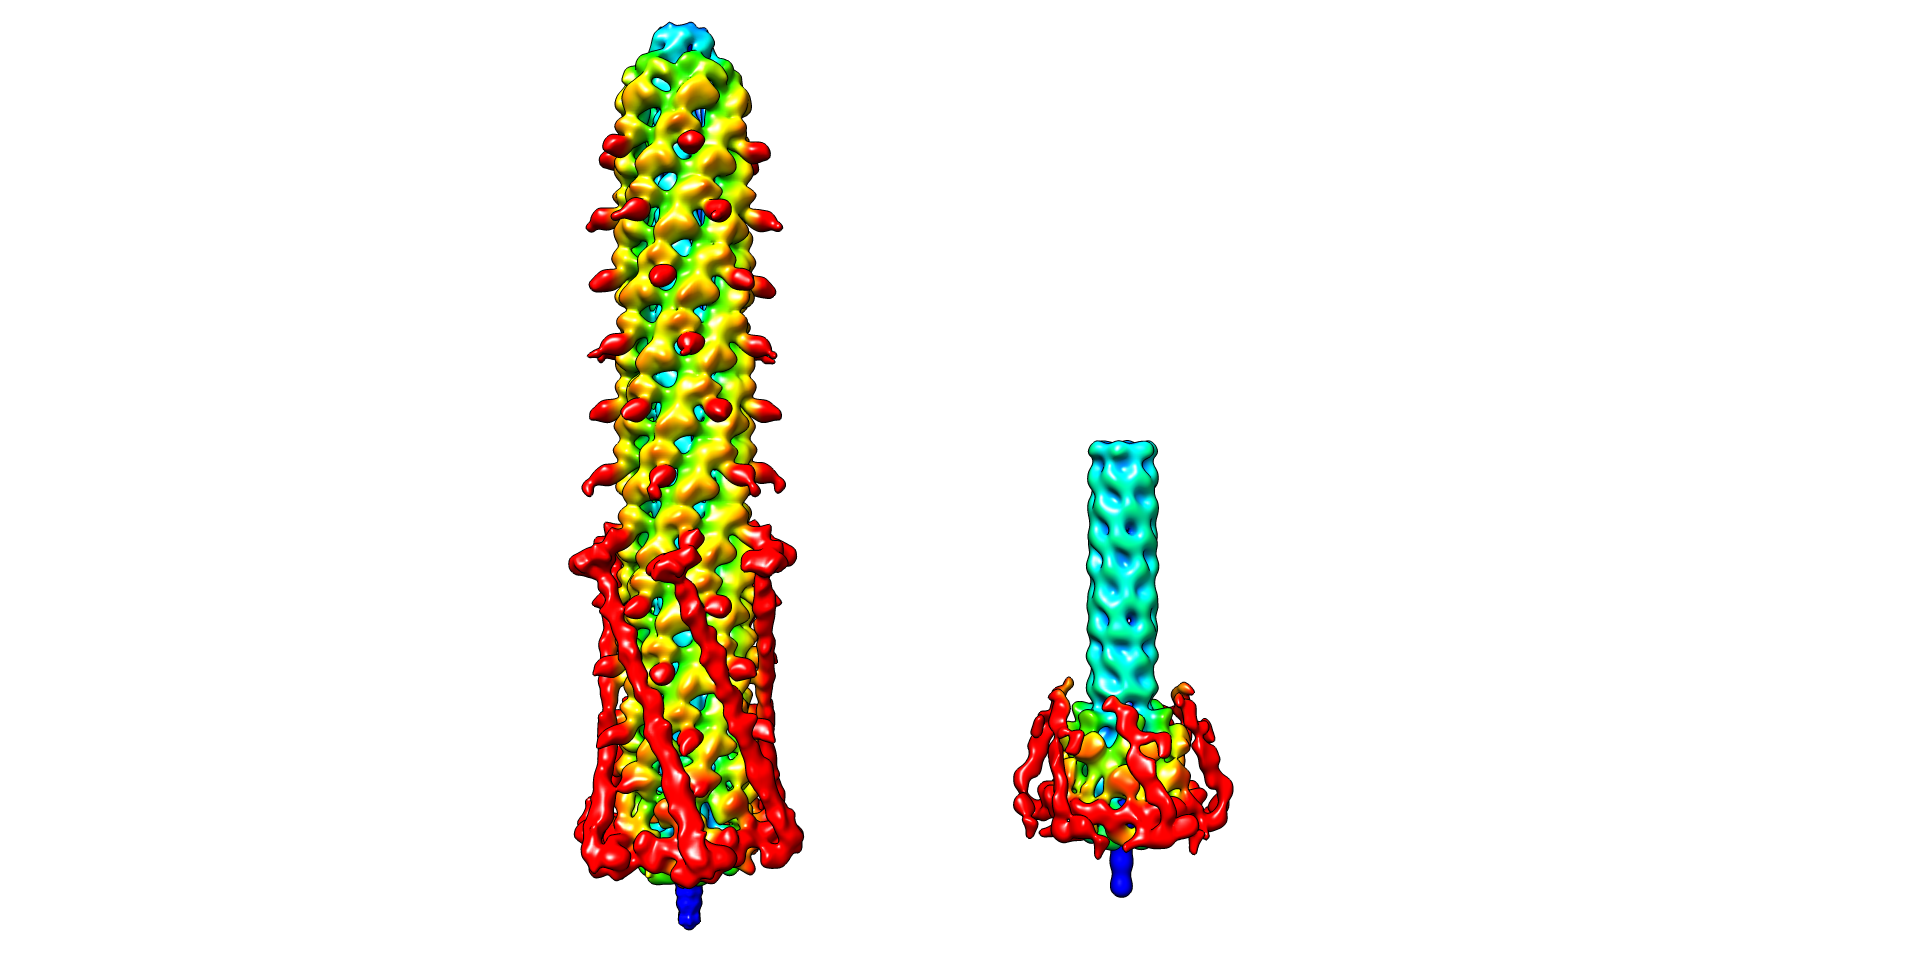
\includegraphics[width=\textwidth, trim={105 7 68 52}, clip]{/Users/joehealey/Documents/Warwick/PhD/Thesis/chapters/intro/img/afp_map_reconstructed.png}
            \captionsetup{singlelinecheck=off, justification=centering, font=footnotesize, aboveskip=15pt}
            \caption{}
            \label{afp3}
        \end{subfigure}%    
  }\cr
}
	\captionsetup{singlelinecheck=off, justification=justified, font=footnotesize, aboveskip=10pt}
	\caption[Antifeeding prophage Electron Density maps from \cite{Heymann2013}]{\textsc{\normalsize The structures of the Antifeeding prophage from \cite{Heymann2013}.}\vspace{0.1cm} \newline \textbf{(A)} The reconstructed 20 \AA{} electron density map for the \emph{S. entomophila} Antifeeding prophage, based upon \cite{Heymann2013}, and reproduced independently from the deposited data under EMDB-2419. All panels in this image are coloured by the distance in \AA{}ngstroms from the centre of rotational symmetry (blue $\leq$ 20\AA \ to red $\leq$100 \AA). Some features of note include the dark red sheath protrusions and the very well defined putative tail fibres folded back against the tube. \textbf{(B)} Various orthogonal views of the tube baseplate/spike and inner core. Note, in particular, a density in the lumenal space in the top left panel. Adapted and reproduced from \cite{Heymann2013}. \textbf{(C)} A ``Tube-Baseplate Complex" which was expressed without any exterior sheath proteins in the same study, revealing further detail of the baseplate complex and the inner sheath.}
	\label{afpstructure}
\end{figure}
}

Despite this extensive study, the EM map that was obtained, displayed in \vref{afpstructure}, is low resolution (at only 20 \AA), and only the gross architecture of the spike and tubes are reliably discernible. This was a substantial improvement over previous iterations however, as the group were able to correct an initial erroneous observation that the tube would have four-fold symmetry, when in actuality, it has six-fold \citep{Sen2010}. Despite this lower resolution, the Afp map does have some unique features, and even advantages over the atomistic R-type pyocin map. As with the other structures that have gone before, the mesh-like structure of the outer sheath is revealed in the obtained density, with the inner sheath visible through `fenestrations' in the outer sheath structure. A baseplate and spike complex is clearly visible, though with no strongly discernible features at this resolution. Attached to the baseplate however, are incredibly distinctive densities for the putative tail fibres, present in a kind of `docked' or `folded' conformation. The fact the tail fibres have been locked in to a prostrate position along the length of the tube, has likely stiffened them, allowing them to be imaged successfully without the averaging effect of tomography blurring them out, as is the case with the structure from \cite{Ge2015}. Indeed, in \vref{afp3}, the lack of the outer sheath stabilising the distal ends of the fibres has resulted in the commonly seen blurring effect. Even at a 20 \AA{} resolution, it is possible to identify a bulbous region at the distal ends of the tail fibres, which is consistent with the trimeric nature of other, more fully resolved, viral adhesion proteins.

Another striking feature of the Afp structure versus the R-type pyocin and the T4 phage, is that the outer sheath appears to more closely resemble that of T4, due to having long sheath protrusions (visible in dark red in \vref{afp1}), than it does the R-type pyocin. This structure, combined with the initial suspicion of four-fold symmetry lead \cite{Sen2010} to conclude that the Afps may represent an evolutionarily distinct sub-type of contractile tail structures. Whether or not this is valid in the context of the protrusions being unusual when compared to the R-type pyocin for example, is not clear without a fully resolved atomistic structure. It is clear that the argument from four-fold symmetry is erroneous in light of the more recent and higher resolution studies of \cite{Heymann2013} however. At present, there is no known functional relevance for these domains.
 
Finally, there is one particularly interesting feature of the EM densities obtained by Heymann and colleagues. In \vref{afp2}, in the top left inset panel, a dark blue density can be seen in the lumen of the central tube. This presents a couple of possible explanations. Perhaps the most likely explanation is that it is artifactual from the averaging process, given that this axial region would not move greatly during tomography, and would thus appear as a static, but blurred, part of the structure.

Alternatively, it is possible there is a structural or biological basis for these densities. As was mentioned in the review of T4, caudate structures are proposed to require a tail `tape measure' protein which extrudes along the length of the growing tail and triggers capping. In T4, this has been proposed to be gp29, and through deletion studies, a similar role was observed for Afp16 \citep{Rybakova2013, Abuladze1994, Katsura1987}. One current theory is that these tape measure proteins exert their effect by lying along the length of the interior of the tube, though there is sparse evidence for this particular mechanism. If this were the case, this density may well correspond to a tape measure protein.

Lastly, the Afps, like the PVCs are thought to package payload effector molecules in to the interior of the tail. This is an intriguing prospect, and would represent the first structural data that attests to this. Given the uniformity of the density along the length of the tube, and its width of only a few \AA{}ngstroms however, the former of these 3 theories seems like the most likely given the information at hand.

In summary, the Afps and PVCs are extremely similar, which is perhaps not unsurprising given their host's similar lifestyles as insect pathogens. However, as this section as highlighted, they are not without differences, corresponding to potentially drastic differences in selection pressure and deployment in the environment. Chief among the differences are the fact that the Afps are plasmid borne, and the PVCs aren't (though perhaps once were). A compelling explanation for significantly different selection pressures is the fact that Afps have been demonstrated to be extremely selectively toxic to only the New Zealand grass grub. The geographic isolation of New Zealand, known for its unusual flora and fauna, may point to a long co-evolution of \emph{S. entomophila} and \emph{C. giveni} which limits the host range. In the recent paper by \cite{Hurst2018}, AfpX was demonstrated to be toxic to the larvae of the Manuka beetle (\emph{Pyronata festiva}), another organism which is endemic to New Zealand, and has yet to be found elsewhere. \emph{Photorhabdus}, by contrast, has demonstrated wide ranging lethality to insects, and is found throughout the world. Lastly, the PVCs are present in various forms, scattered throughout \emph{Photorhabdus} genomes, and this alone has potentially lead to enormously different selection pressures (due to their paralogy), and potentially morphology - whereas \emph{Serratia} is limited to only 2 examples (and still only a single operon per genome).


\subsubsection{Of PVCs and Type VI Secretion Systems}\label{t6ss}
Now that the closest cousins of the PVCs have been discussed, in the form of the AFPs and R-type pyocins, moving back up in complexity brings us back to another well studied biological complex - the Type VI Secretion System (T6SS). \cite{Bonemann2010} were the first to draw parallels between the T6SS and the PVCs, realising that the contractile, puncturing mechanism of the system placed it in a `supergroup' of contractile injection systems.

 The T6SS is just one of a family of secretion systems which have come to be recognised in bacteria, as a mechanism for the organism to communicate with, and manipulate, the extracellular environment, including other organisms. At the time of writing, at least 9 ``Type \textbf{$x$}" secretion systems have been described (numbered in Roman numerals I to IX), each of which has been studied to a differing degree and there are great number of reviews covering some or all of them to date \citep{Dalbey2012,Chang2014a, Bleves2010, Desvaux2009, Abby2016, Costa2015, Goulet2004, Remaut2008, Gerlach2007, Abdallah2007, Green2015}. The ``Type \textbf{$x$}" secretions systems are specialised bacterial structures, and are distinct from the Sec and Tat secretion systems which are present in all 3 domains of life, meaning bacteria exhibit a dizzying array of secretion mechanisms \citep{Green2015}. Discussions of secretion systems are quite `murky waters' however, as they are not all related, despite being named as if they are `shades of grey' with respect to each other. As the details of all the secretion systems are not wholly pertinent to discussions of the PVCs, the depth will be left to the aforementioned reviews. This section will highlight the different types and diversity of known secretion systems, and will then proceed to cover the Type VI secretion system in depth.

\myparagraph{The ``Type \textbf{$x$}" Secretion System repertoire}
Briefly, the T1SS, is a translocator comprised of 3 proteins which is able to secrete a wide variety of bacterial proteins with a wide size range, the one of the largest being the LapA adhesion protein from \emph{Pseudomonas fluorescens}, at an impressive 520 kDa \citep{Boyd2014}. One of the most commonly transported proteins are toxins of the RTX family \citep{Delepelaire2004}. Unlike the other secretion systems, Type I is related to the general class of ABC transporters which are ubiquitous efflux pumps for antibiotics and other small molecules, and is entirely independent of the Sec system, not requiring a first translocation of cargo to the periplasm, though cargoes do require a chaperone.

The Type II Secretion system (T2SS) is a common Gram negative secretion system, and has been studied extensively in a number of human pathogens including \emph{Vibrio} and \emph{Pseudomonas}, though it is not ubiquitously present in Gram negatives \citep{Douzi2012}. The system can be divided in to 4 primary components, though the structure as a whole is a large multipartite protein complex. The inner membrane complex and outer membrane complex are connected by a `pseudopilus' spanning the periplasm, so called as it is made up of a number of proteins resembling pilins \citep{Korotkov2012}. Finally, a crucial hexameric secretion ATPase is associated with the inner membrane complex, and is responsible for the synthesis and dismantling of the pilins, which provides the mechanistic basis for secretion \citep{Lu2013}. Type II is Sec or Tat dependent, and exports a variety of protein cargoes, which often include toxins and degradative enzymes such as proteases and lipases associated with bacterial infection \citep{Korotkov2012}.

An unusual version of a secretion system, and another very well studied apparatus, the Type III Secretion System is quite similar to a PVC in its role as an anti-eukaryotic needle complex delivery system. Homologous to the basal body of the bacterial flagellum \citep{Aizawa2001}, the T3SS is another molecular syringe, but membrane bound. The Type III is used by bacteria to directly inject effector proteins in to the interior of target eukaryotic cells, making it a potent and widely utilised virulence factor \citep{AbuHatab1998} - with examples having been found in \emph{E. coli}, \emph{Shigella}, \emph{Salmonella}, \emph{Vibrio}, \emph{Burkholderia}, \emph{Yersinia}, \emph{Pseudomonas}, as well as a number of plant-associated species such as \emph{Rhizobium}, \emph{Erwinia}, \emph{Ralstonia} and \emph{Xanthomonas}, and more besides. By forming a continuous pore, through the needle bore, from the cytosol of the bacterium to the target cell, Type III is completely Sec/Tat independent. The similarity to the flagella continues in the needle body, as this is homologous to the flagella hook \citep{Lane2007}. Comparable in complexity to the flagella also, the T3SS is comprised of around 30 distinct proteins, making the T3SS among one of the most intricate secretion systems \citep{Green2015}.

Like the T3SS, the Type IV Secretion System is a relative of another fundamental bacterial `appendage' - the conjugation pilus, used by bacteria to exchange genetic material. Unlike the conjugation machinery however, the T4SS is capable of translocating protein (as well as nucleic material). The Type IV system was discovered originally in \emph{Agrobacterium tumefaciens}, the long-used tool for genetic manipulation of plant species, and is the mechanism by which the bacterium actually exerts its modifying effects. Thus, the \emph{A. tumefaciens} system in particular, has become the model for T4SS structure and function studies \citep{Bundock1995}. As with the Type III, the `injectisome' nature of the T4SS means that it is Sec/Tat independent. However, there are competing theories as to whether the T4SS simply acts as a harpoon, to pull 2 cells in to close register, and translocation occurs in a still as-yet-undetermined manner, or actually forms a continuous channel from cytosol to cytosol, as in the T3SS \citep{Christie2005, Green2015}.

Unique among all the secretion systems, The Type V Secretion System is an auto-transporter, rather than a channel for other proteins (though it is capable of exporting others as well in some cases), and requires no ATP to function \citep{Thanassi2005}. Proteins that comprise the T5SS class contain a C-terminal region which inserts into the outer membrane (after translocation via Sec), forming a $\beta$-barrel, and they then proceed to translocate the N-terminal passenger effector domain, which is proteolytically cleaved. The $\beta$-barrel remains in the outer membrane until it is lost or recycled, potentiating the passage of other substrates, once the passenger domain is no longer causing an obstruction. Continuing the theme from the other secretion systems, most known T5SS secreted proteins are virulence factors and host modulators \citep{Green2015}.

Skipping over the Type 6 for the moment, in favour of a more full review in this section, the Type VII secretion system is unlike the other secretion systems mentioned so far, as it (to date) has only been found in Gram positive bacteria such as the \emph{Corynebacteria} and \emph{Actinobacteria}, and most famously in the \emph{Mycobacteria} \citep{Ates2016}. Gram positive bacteria, due to their (typically) single cell membrane, and thickened cell wall, have different challenges to overcome when secreting molecules in to the extracellular milieu \citep{Green2015}. It is thought that the T7SS is widespread amongst Gram positives, with Type VII-like operons and orthologues having been detected in \emph{Staphylococcus aureus}, and \emph{Bacillus subtilis}, the well known model organism for Gram positives. The structure and function of the complex and its constituent proteins are not yet well understood. There is a large inner membrane complex, formed of at least 5 distinct proteins, which is thought to provide a channel for substrates, though there are a number of additional proteins for which roles have not yet been elucidated. Since the formation of a pore in the membrane would not allow substrate passage beyond the interior face of the cell wall, it seems likely that some or all of these remaining proteins serve to facilitate this last hurdle in some way. Though extremely distant in terms of any genetic relation (if any), there is an interesting parallel between the PVCs, and the T7SS in \emph{M. tuberculosis}; namely, that the \emph{Mycobacteria} harbour up to 5 T7SSs, as \emph{Photorhabdus} habours up to 6 PVCs, and not all of these are present in every genome of the species \citep{Bottai2017}. The T7SS is known to function mostly (though not entirely) in virulence, and this potentially speaks to the same diversification seen in the PVCs, honing multiple copies of highly effective virulence factors to become a more effective pathogen, or cope with varying environmental conditions.

Historically, the Type VIII system has been referred to as the `extracellular nucleation-precipitation pathway' (ENP) and the switch to T8SS was proposed by \cite{Desvaux2009}. The structure of the T8SS was resolved by \cite{Goyal2014}, and comprised a fairly typical looking membrane 36-strand $\beta$-barrel which is embedded in the outer membrane. The T8SS, therefore, is Sec/Tat dependent. Unlike the majority of the other secretion systems, the Type VIII is thought to be limited to a single substrate. It is responsible for secreting proteins known as `curli' - a primary component of the extracellular matrix of many \emph{Enterobacteriaceae} \citep{Barnhart2010}.

The Type IX Secretion System is one of the most recently discovered secretion systems with only a single structurally resolved component. To date, it has only been detected in certain species of the \emph{Bacterioidetes} phylum, after being originally discovered in the oral pathogen \emph{Porphyromonas gingivalis}. The T9SS has been demonstrated to be implicated in 2 distinct lifestyle roles, both gliding motility and as a pathogenic virulence factor/weapon, though with unknown functional bases. It is dependent on the Sec system, providing only carriage across the outer membrane. Originally termed the PorSS system, 18 proteins are known to be essential, but roles for all of them remain elusive, while as many as 29 proteins are hypothesised to be involved in some way, making the T9SS comparable in complexity to the Type III and Type VI \citep{Lasica2017a}


So, finally returning to the Type VI secretion system, as with the T4 capsid, this section is not going to dwell extensively on the membrane associated apparatus of the Type 6 Secretion System, since the PVCs appear to be secreted/released by lysis, and thus contain no analogous structures (and the membrane complex is still not well understood). Instead the similarities of the PVCs and the T6SS in terms of their putative translocation role and thus their spikes and tubes (i.e. as contractile nanomachines) will be the focus.

The T6SS has been identified in about 25\% of all Gram negative sequences \citep{Basler2015a}, and despite being the most recently discovered secretion system (first being dubbed the T6SS in 2007) \citep{Nguyen2018, Pukatzki2007, Cascales2012}, it has rapidly become quite well studied, with a significant amount of structural resolution completed to date \citep{Mougous2006a}. It has been shown that the T6SS is encoded by a highly conserved 13 gene cassette, which forms the core of the system, with a number of accessory proteins. The presence of these accessory proteins can vary by organism, but are typically well conserved when they are found \citep{Basler2015a}.

Among all the secretion systems, the Type VI is unique in a couple of primary ways. Firstly, it is the only secretion system with a contractile mechanism, as with T4 and the pyocins etc., as well as being the only system which delivers effectors to both other bacteria, and eukaryotic targets. Thus, the T6SS is an intricate but highly versatile nanosyringe complex - essentially an ``upside down myophage in the membrane" - and is employed by a large number of bacteria in their pathogenic, but also community roles \citep{Russell2014}. 


\vspace{0.1cm}
\begin{figure}[h]
\centering
    \begin{subfigure}[b]{0.481\textwidth}
        \centering
        {%
\setlength{\fboxsep}{0pt}%
\setlength{\fboxrule}{1pt}%
        \fbox{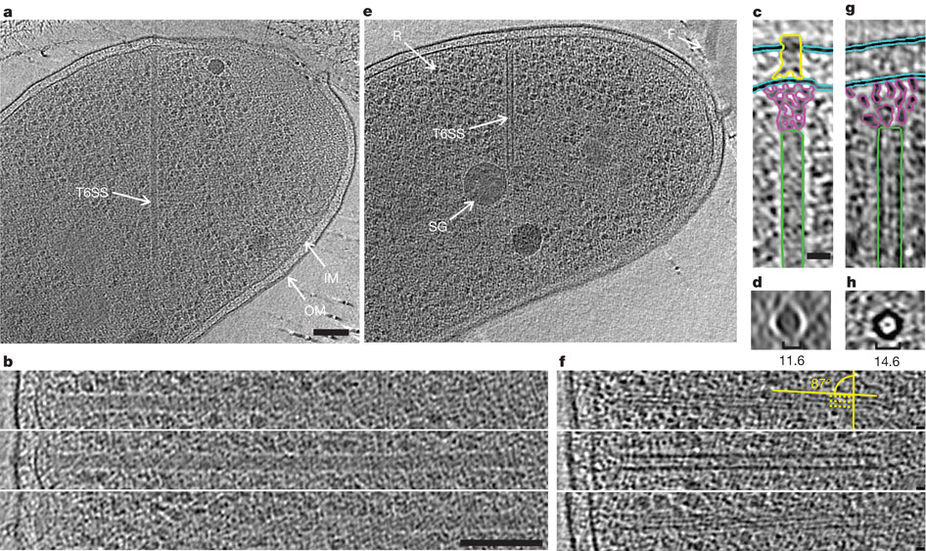
\includegraphics[width=\textwidth, trim={0 230 200 20}, clip]{/Users/joehealey/Documents/Warwick/PhD/Thesis/chapters/intro/img/t6ss_in_cell.jpg}}
            }%
    \end{subfigure}%
    \begin{subfigure}[t]{0.499\textwidth}
        \centering
        {%
\setlength{\fboxsep}{0pt}%
\setlength{\fboxrule}{1pt}%
        \fbox{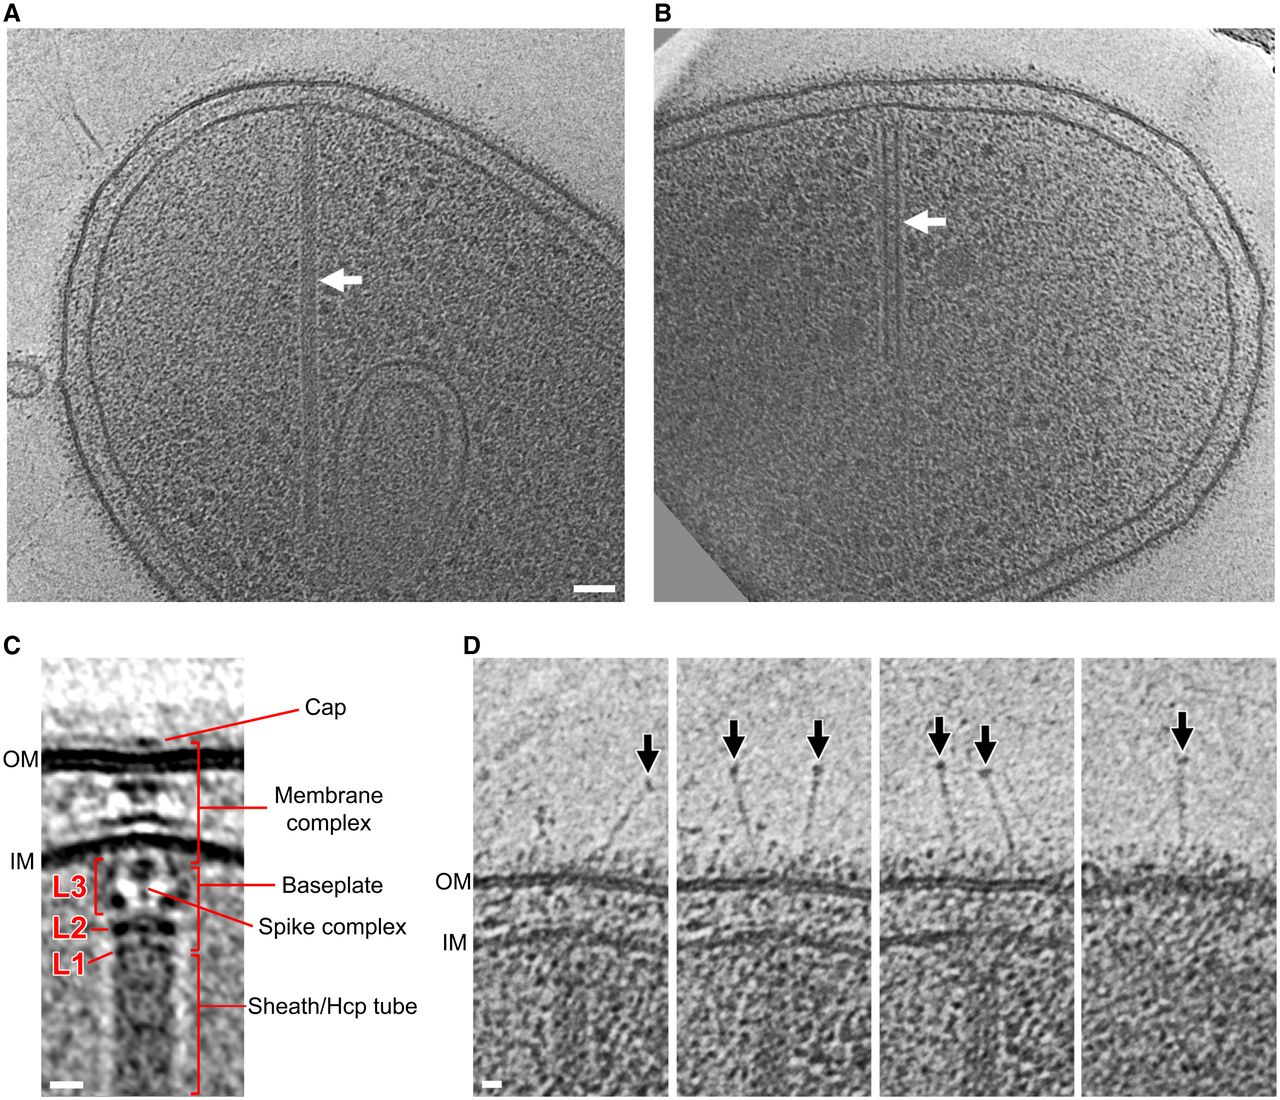
\includegraphics[width=\textwidth, trim={0 1 50 160}, clip]{/Users/joehealey/Documents/Warwick/PhD/Thesis/chapters/intro/img/t6ss_annotated}}
        }%
        \end{subfigure}%
	\captionsetup{singlelinecheck=off, justification=justified, font=footnotesize, aboveskip=10pt}
	\caption[Electron micrographs of the Type VI Secretion System]{\textsc{\normalsize Electron Micrographs of the Type VI Secretion System.}\vspace{0.1cm} \newline The left panel shows 2 EMs of the T6SS, and displays the enormous magnitude and variability in size of the tube complex, in the left most inset, the T6SS is labelled. In the right inset, the T6SS is labelled again, along with putative ribosomes (R), a flagellum (F), storage granule (SG), and the inner and outer membranes (IM/OM) Adapted and reproduced from \cite{Basler2012}. The right hand panel shows an annotated close up of the T6SS membrane complex. Labelled are the Inner and outer membranes (IM/OM), cap, membrane complex, tube, spike complex, baseplate, and the black arrows in the left most tryptic identify `antennae', purported to be the T6SS equivalent of phage tail fibres. L1-L3 demarcate different layers of EM density. Adapted and reproduced from \cite{Chang2017}.}
	\label{t6ssEMs}
\end{figure}


Though its role in pathogenesis was determined first by \cite{Pukatzki2006} whereby the T6SS locus of \emph{Vibrio cholerae} was demonstrated as enabling the bacterium to resist predation by the model amoeba species \emph{Dictyostelium discoideum}, the T6SS is deployed predominantly against prokaryotic targets \citep{Green2015, Russell2014, Hood2010}. A wide variety of roles for the T6SS have been postulated, both in antagonism (which is well documented) and in synergism. The diversity of competition against which the T6SS might be deployed `in the wild' is thought to underscore the rampant diversity that is seen between homologues. Furthermore, the need for competition between extremely closely related species and even strains, is driving the underlying selective pressure that has resulted in an enormous variety of Type VI effectors \citep{English2012, Russell2012}. The effector/immunity protein pairs that typify Type VI effectors have been suggested to act in a number of subtle ways, given this diversity. A rather ingenious mechanism has been proposed, wherein target cells which harbour a cognate immunity protein for a given toxin, utilise the toxin-immunity complex as a signalling molecule. Thus, those which have the correct immunity protein receive a signal, whereas those that don't, receive an antagonistic `message' - as if the bacteria are mailing each other `booby trapped' messages \citep{Russell2014}. Among other synergistic roles, the T6SS has been implicated in: the determination of self vs. non-self in \emph{Proteus mirabilis} \citep{Gibbs2008, Wenren2013}; triggering `assisted suicide' in phage infected cells inter-cellularly, in a manner analogous to that shown for `classic' Toxin-Antitoxin systems \citep{Hazan2004}; and as a method for overcoming the outer membrane to deliver cell wall remodelling factors which have been shown in other systems to `resuscitate' neighbouring cells from viable-but-non-cultureable states \citep{Downing2005, Mukamolova2006}.



\begin{figure}[p]
\thisfloatpagestyle{augment}
\centering
\tabskip=0pt
\valign{#\cr
\hbox{%
    \begin{subfigure}[t]{0.42\textwidth}
        \centering
         \begin{tabular}{c}
            \rotatebox{90}{\raisebox{-.5\height}{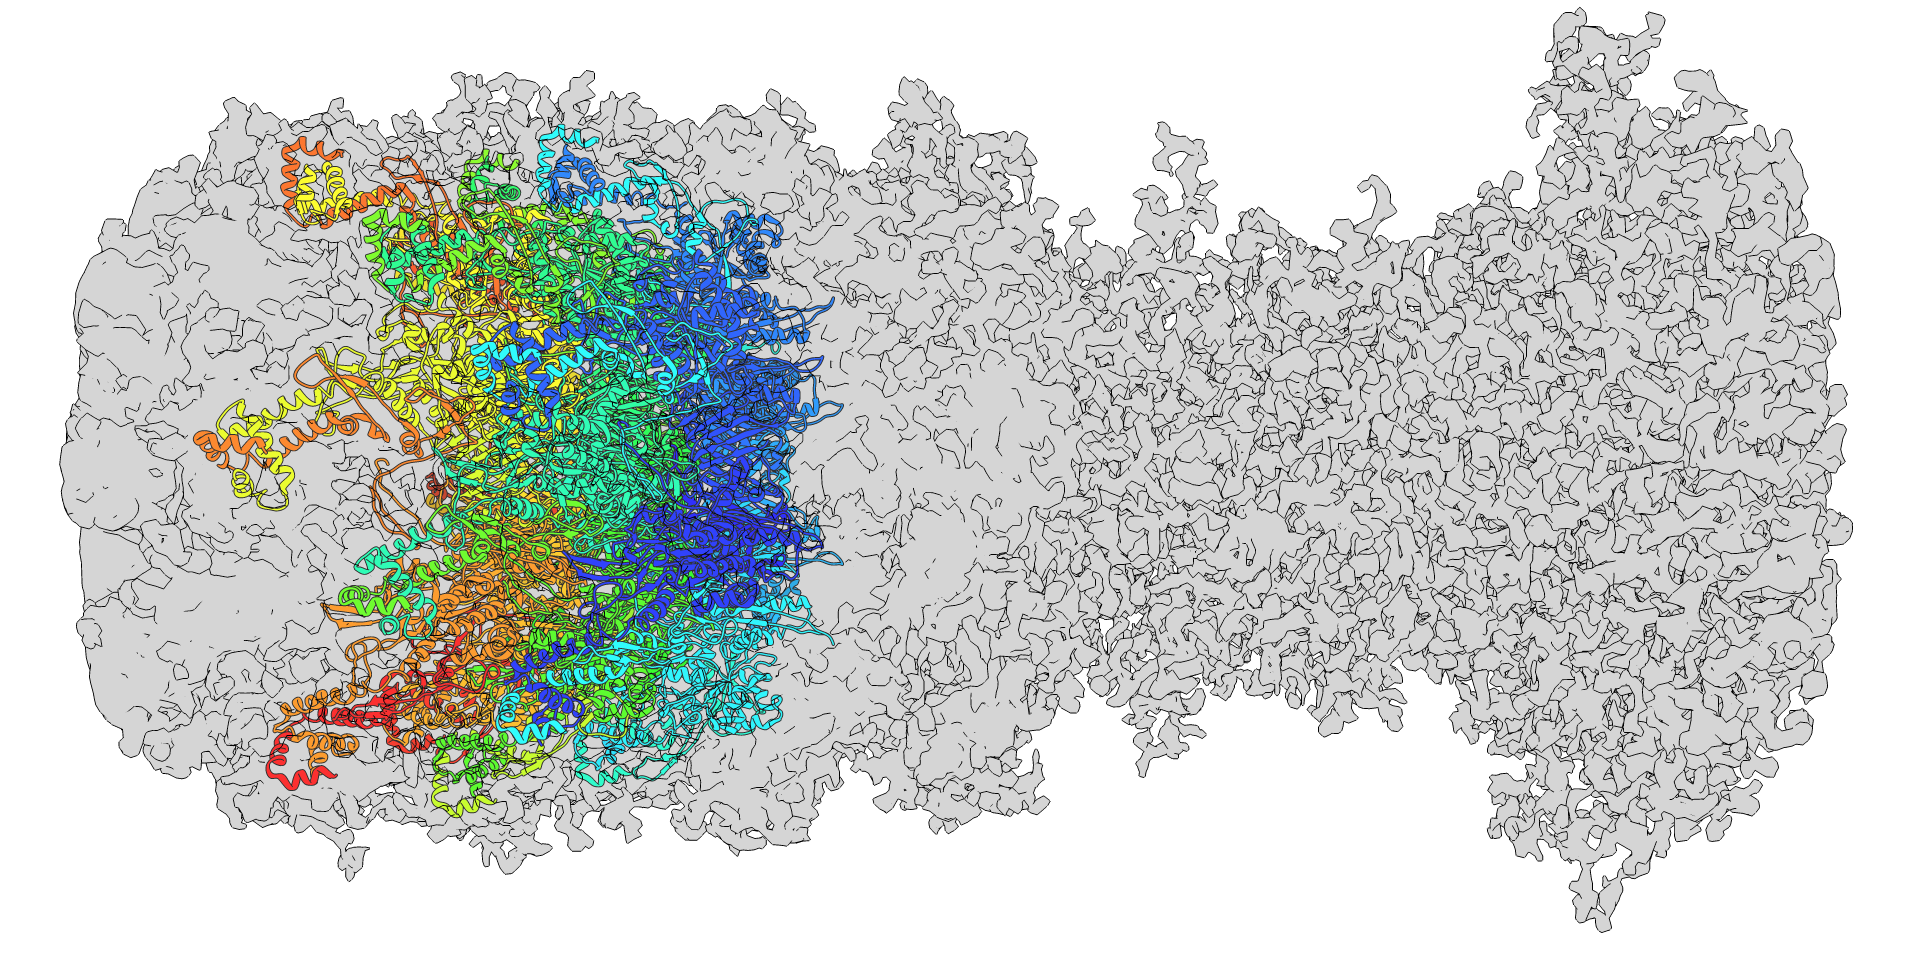
\includegraphics[width=1.65\textwidth, trim={20 0 10 0}, clip,]{/Users/joehealey/Documents/Warwick/PhD/Thesis/chapters/intro/img/t6ss_distal_grey_flat.png}}} \\
            \rotatebox{90}{\raisebox{-.5\height}{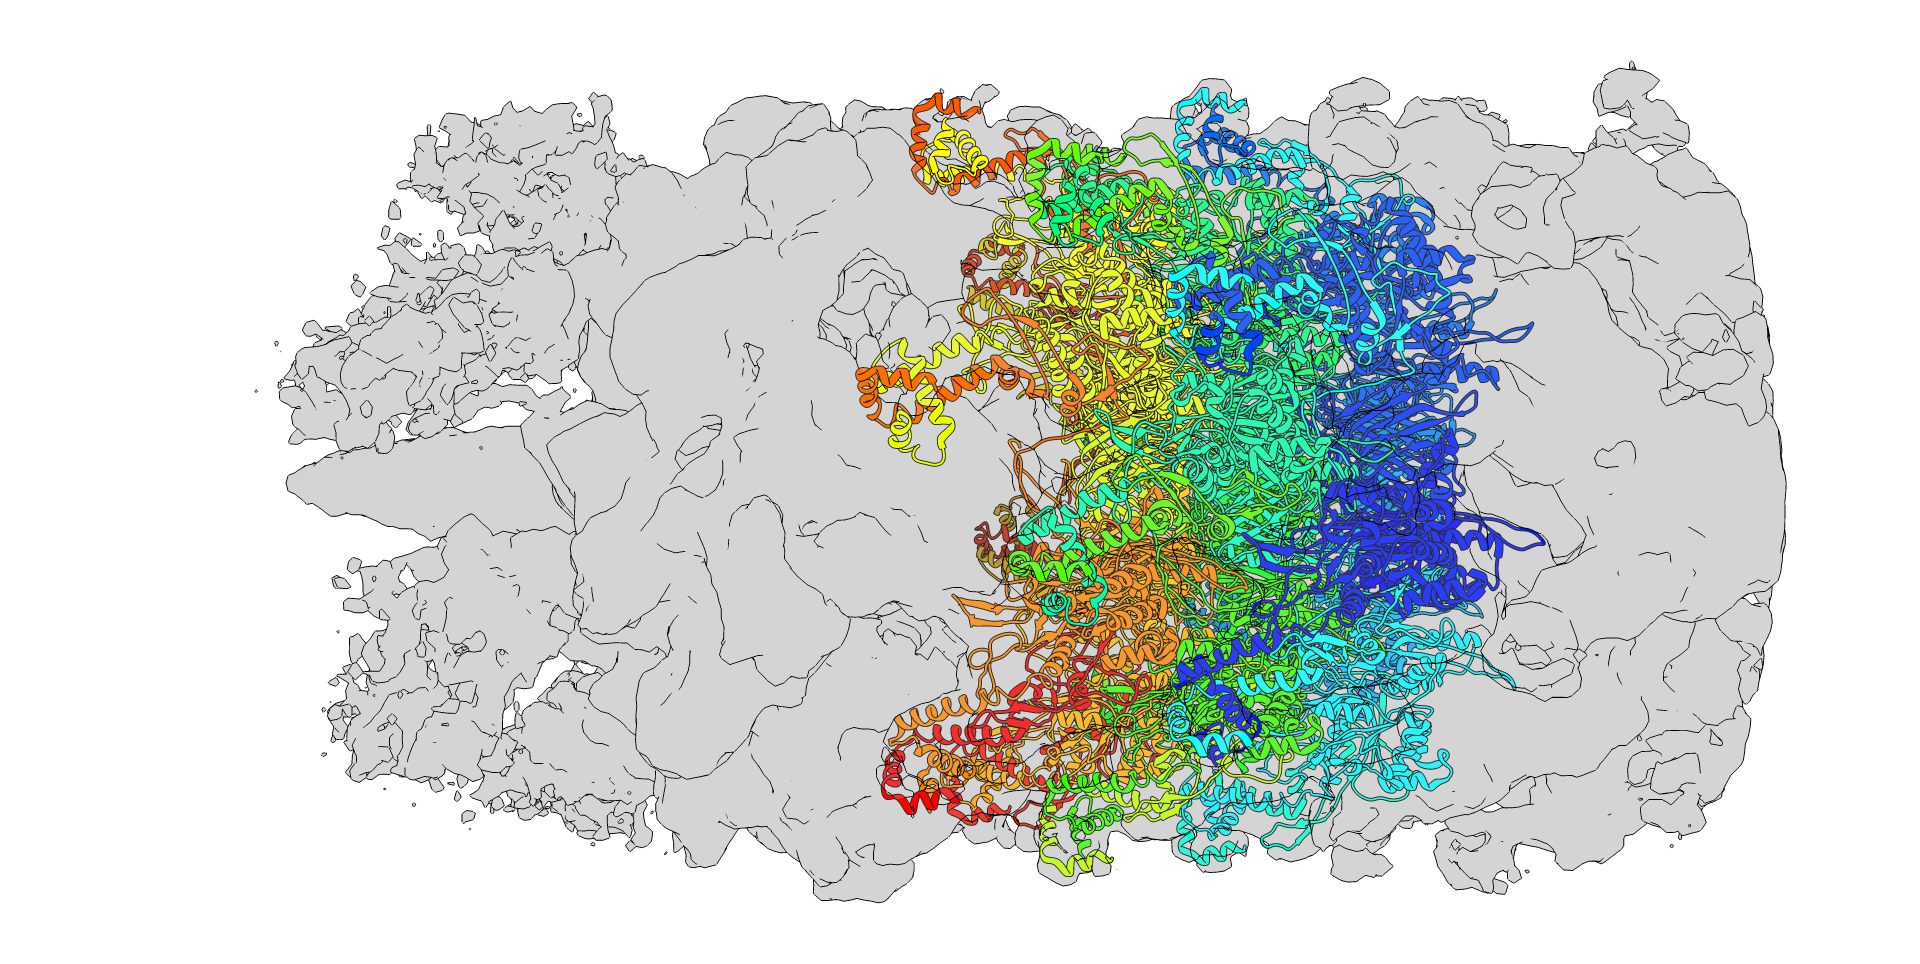
\includegraphics[width=1.38\textwidth, trim={30 0 30 0}, clip]{/Users/joehealey/Documents/Warwick/PhD/Thesis/chapters/intro/img/t6ss_proximal_grey_flat.png}}} \\
          \end{tabular}
         \put(-171,-15){
                 \rotatebox{-85.5}{
                     \obscure[gray]{0.02cm}{5.1cm}\obscure{0.5cm}{5.1cm}\obscure[gray]{0.02cm}{5.1cm}}
                 }
%         \put(-129,-25){\rotatebox{5}{\footnotesize$x$ hundred nanometres \{}}
        \captionsetup{singlelinecheck=off, justification=centering, font=footnotesize, aboveskip=10pt}
        \caption{}
        \label{tss1}
    \end{subfigure}%
}\cr
\noalign{\hfill}%
\hbox{%
    \begin{subfigure}{0.58\textwidth}
        \centering
        \vspace{1cm}
          \begin{tabular}{lr}
            \raisebox{-.5\height}{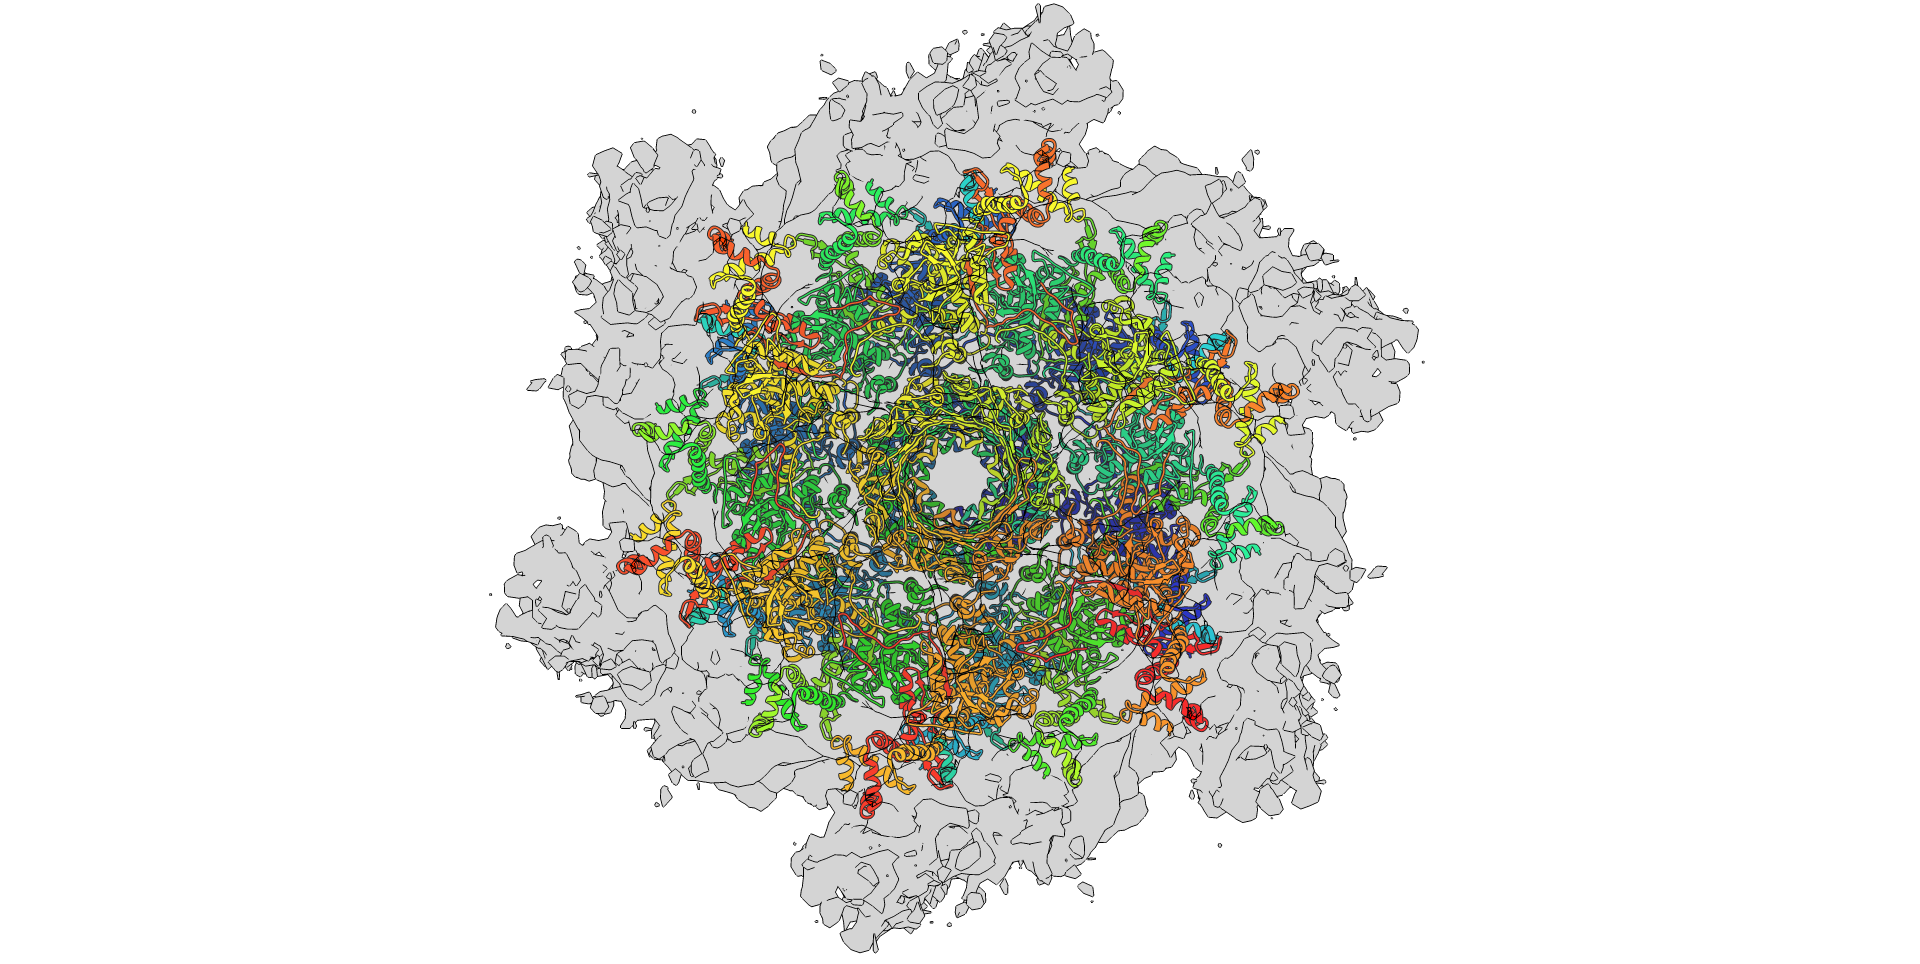
\includegraphics[width=0.5\textwidth, trim={55 0 55 0}, clip,]{/Users/joehealey/Documents/Warwick/PhD/Thesis/chapters/intro/img/t6ss_proximal_grey_flat_bottom.png}} &
            \raisebox{-.5\height}{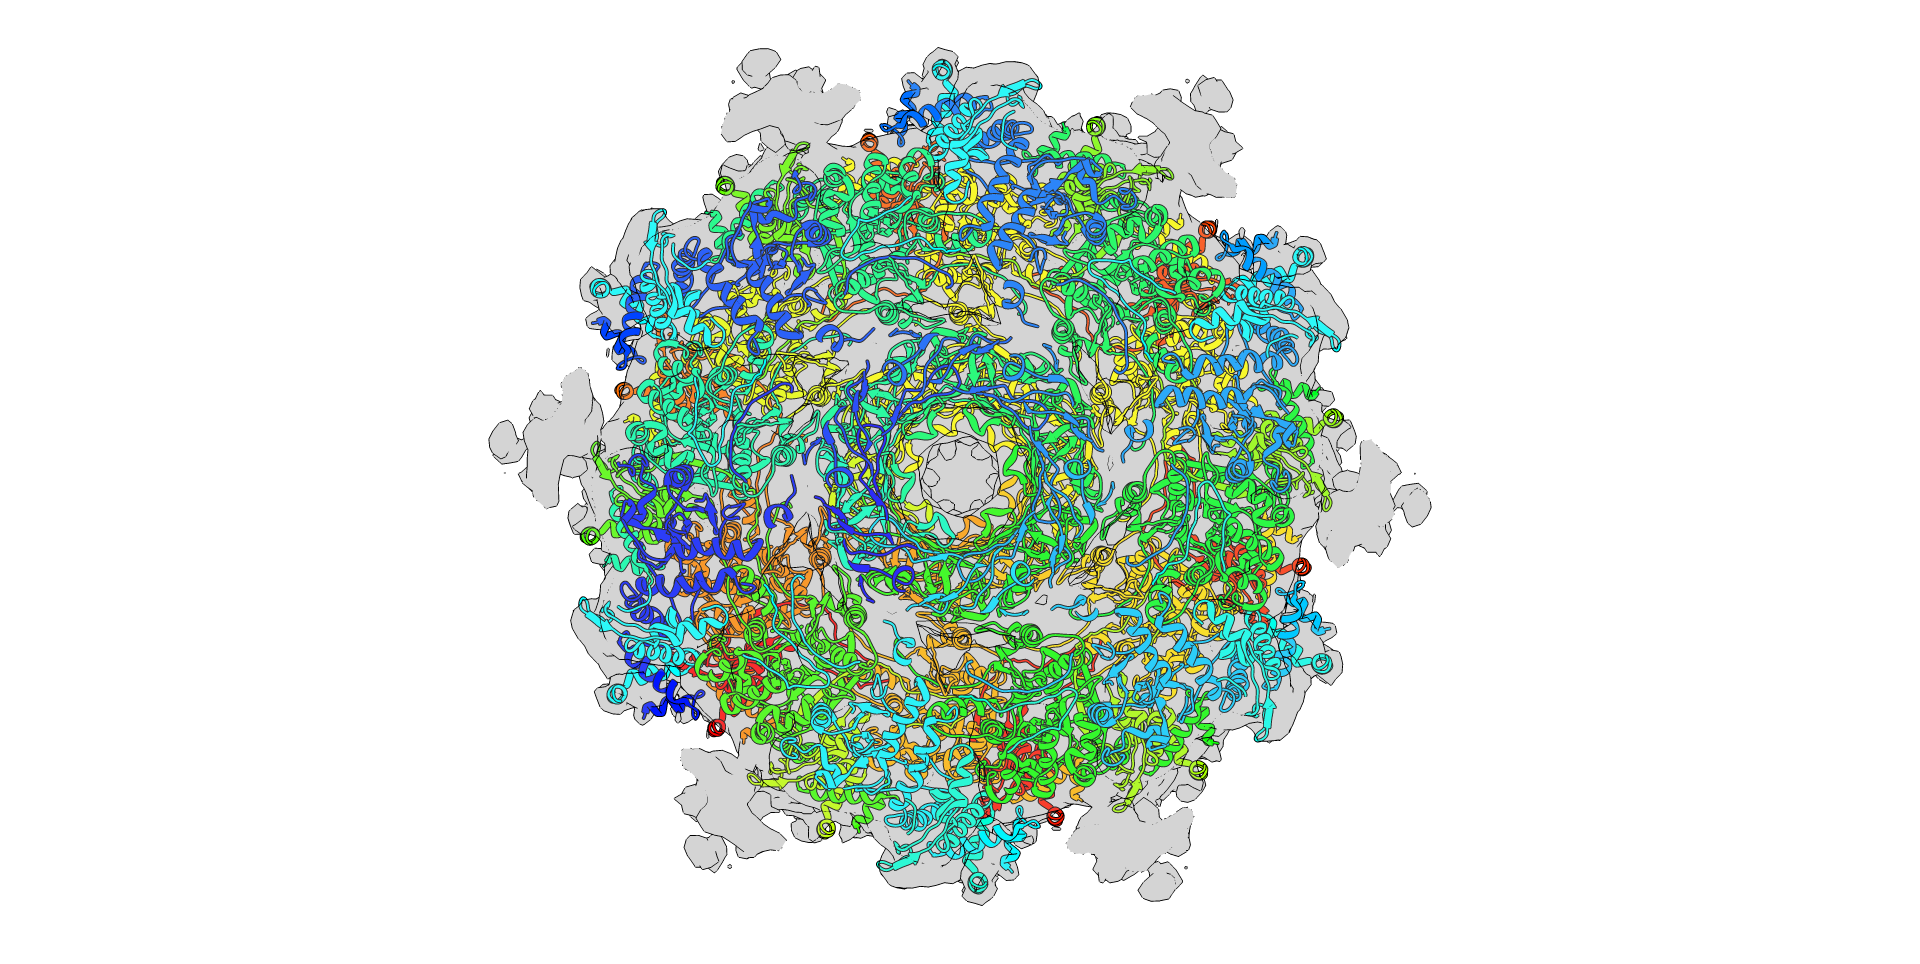
\includegraphics[width=0.5\textwidth, trim={55 0 55 0}, clip]{/Users/joehealey/Documents/Warwick/PhD/Thesis/chapters/intro/img/t6ss_proximal_grey_flat_topslice.png}} \\[2ex]
            \multicolumn{2}{c}{\raisebox{-.5\height}{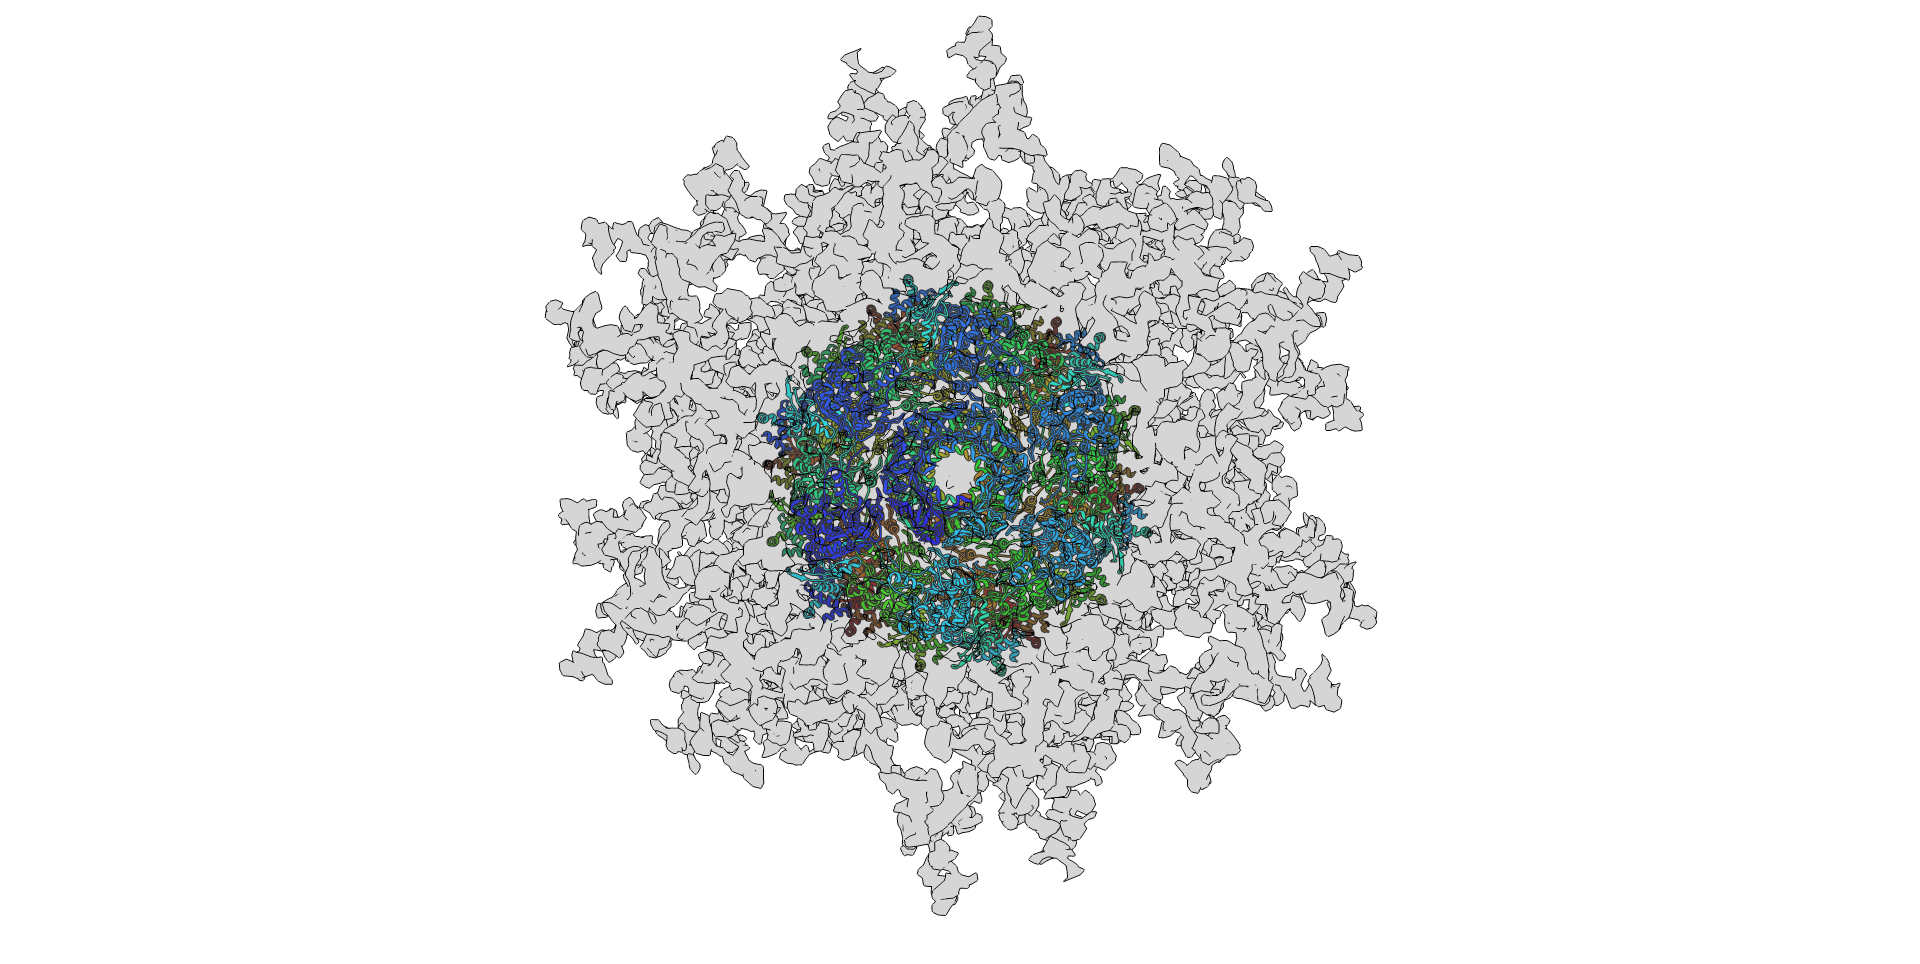
\includegraphics[width=0.6\textwidth, trim={55 0 55 0}, clip]{/Users/joehealey/Documents/Warwick/PhD/Thesis/chapters/intro/img/t6ss_distal_grey_flat_top.png}}} \\
     \end{tabular}
        \captionsetup{singlelinecheck=off, justification=centering, font=footnotesize, aboveskip=5pt}
        \caption{}
        \label{t6ss2}
        \end{subfigure}%
}\vfill
    \hbox{%
        \begin{subfigure}[t]{0.58\textwidth}
            \centering
            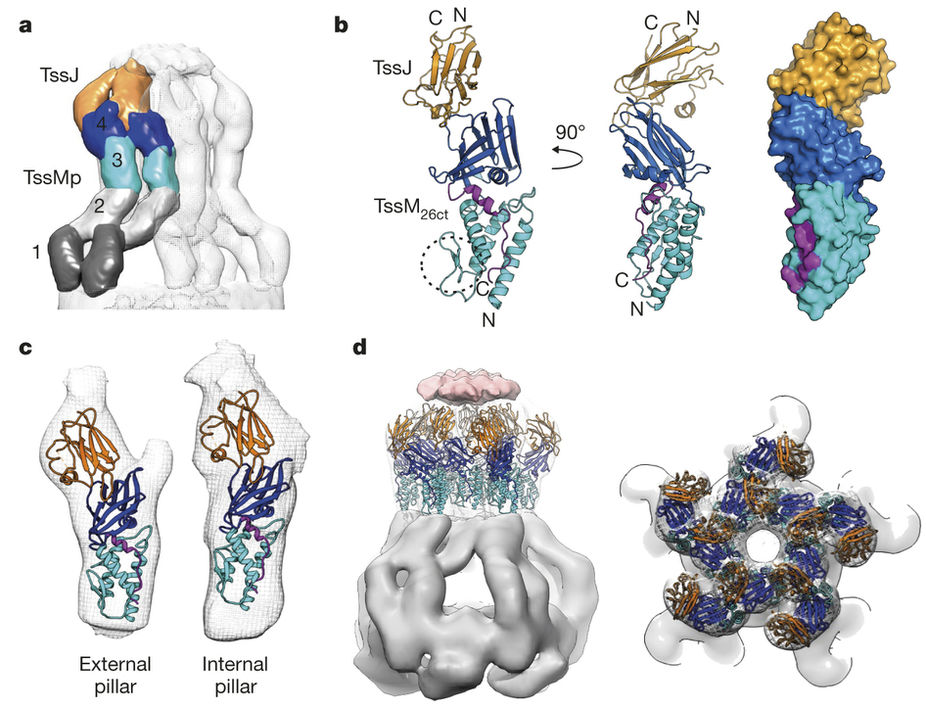
\includegraphics[width=\textwidth, trim={325 -100 0 360}, clip]{/Users/joehealey/Documents/Warwick/PhD/Thesis/chapters/intro/img/t6ss_tmc.jpg}
            \captionsetup{singlelinecheck=off, justification=centering, font=footnotesize, aboveskip=5pt}
            \caption{}
            \label{t6ss3}
        \end{subfigure}%    
  }\cr
}
\vfill
	\captionsetup{singlelinecheck=off, justification=justified, font=footnotesize, aboveskip=5pt}
	\caption[Type VI Secretion System Structures]{\textsc{\normalsize The structures of resolved components of the Type VI Secretion System.}\vspace{0.1cm} \newline \textbf{(A)} The EM density for the proximal and distal ends of the pre-contraction Type VI secretion tube. Figures were reproduced independently from the deposited data under EMDB-3878 and 3879 from \cite{Nazarov2017}. The density shows the spike complex and a distal cap like structure as well as the atomic architecture of the sheath. \textbf{(B)} Top left - a bottom view of the proximal end of the tube (spike toward the viewer). Top right - a slice through the centre of the tube, demonstrating well the dodecameric spokes in different planes. Middle bottom - a view from the top of the cap-like protrusion density. All also reproduced independently from \cite{Nazarov2017} EMDBs 3878/3879. \textbf{(C)} The 12 \AA{} map of the membrane complex of the system, with a TssM/J complex fitted in to the upper arches. Adapted and reproduced from \cite{Durand2015}.}
	\label{t6ss_structure}
\end{figure}

\clearpage

The T6SS is broadly divided in to approximately 4 structural complexes - a contractile tube (one could make the case that the spike complex forms a 5th component), a baseplate complex, a transmembrane domain, and associated soluble proteins. As a contractile tail system it, of course, exhibits a pair of concentric tubes, the inner of which is tipped with a spike complex, as with the other systems discussed so far. The inner tube is comprised of Hcp (``Haemolysin coregulated protein") hexameric toroids; Hcp being the ortholog of gp19/Afp 1 \& 5. The Hcp tube is approximately 80 \AA{} in outer diameter, with an inner lumenal diameter of roughly 40 \AA{} \citep{Mougous2006a}. Multiple crystal structures of Hcp orthologues and paralogues have been solved, and reveal the same overall gross architecture, though there is often some flexibility in the secondary structure and even more so in sequence. The inner tube appears more similar to that of R-type pyocins and the PVCs as it doesn't exhibit a helical turn, instead just being direct stacks of Hcp \citep{Silverman2012a, Mougous2006a, Osipiuk2011}. It was originally thought that Hcp itself was a secreted molecule, though without a known function, though it is now realised that the Hcp proteins may dissociate when puncturing in to the interior of another cell, and the filament of the tube is exposed to the extracellular environment during contraction. Thus, any dissociated Hcp monomers are essentially secreted `inadvertently', though this could obviously not be determined in the early experiments. In the T6SS of \emph{Edwardsiella tarda} it was also observed that the VgrG spike protein is secreted, but if either \emph{Hcp} or \emph{VgrG} homologues were knocked out, neither could then be detected in the supernatants of T6SS$^+$ cultures. The generally accepted, and likely, explanation for this is that Hcp tubules only assemble and secrete/puncture through the membrane if first polymerised off the VgrG baseplate hub analogous structure, as is the case in the T4 phage. Similarly, VgrG can only be detected in supernatants if Hcp is present to form the tube to which VgrG binds, and then is carried across the cell envelope by `riding' the tube out of the cell \citep{Pukatzki2007, Zheng2007, Hachani2011}. High resolution microscopic studies with the help of fluorescent constructs have been able to demonstrate that multiple T6SS complexes can be carried by a cell at once, and the tube complexes can extend many hundreds of nanometers, deep in to the cytosol of the cell - even reaching the opposite cell envelope \citep{Nguyen2018, Chang2017}.

Unlike the other systems mentioned up to this point, the exterior sheath of the T6SS differs quite substantially in structure, despite still forming a contractile system. As can be seen in the upper right panel of \vref{t6ss2}, the outer sheath is actually a dodecameric toroid, comprised of 2 different proteins: TssB and TssC. Type 6 secretion proteins have been given alphabetic nomenclature preceded by ``Tss" (Type six subunits), as such, the outer 2 sheath proteins for example, are termed TssB/C, and though unrelated, would be the structural orthologues of gp18 in T4. TssB is a smaller protein of around 18 kDa, and TssC comprises the bulk of the tube at $\approx$55 kDa. Together they form an alternating dodecameric ring which is approximately 240 \AA{} across in the extended state and 290 \AA{} in the contracted form, with an inner diameter of 80\AA{} before contraction, and approximately 110 \AA{} post-contraction (in the \emph{V. cholerae} T6SS structure) \citep{Cascales2012, Wang2017, Kube2014a}. If one were to think of the ring as an analog clock face, a TssB monomer would occupy all the odd numbers, and a TssC monomer would occupy all the even positions \citep{Kube2014a}. In the extended form, the sheath has a 38 \AA{} rise, and a 23.6$^{\circ}$ twist, and this shifts to a 15.8 \AA{} rise and 29.4$^{\circ}$ twist after contraction \citep{Wang2017}. Both subunits appear to contribute to protrusions around the exterior of the tube which form a left-handed helical series of ridges. This is not a trivial observation either, as this is the opposite handedness to the T4 phage tail. Such a dramatic rearrangement in structure further underscores the hypothesis/observation that T6SS outer sheaths are unrelated in origin to T4 phage \citep{Kube2014a}. As is the case with the PVCs and Afps, one of the most conserved proteins appears to be a ClpV AAA+ family ATPase. These are typically protease enzymes which take their name from being ``ATPases Associated with various cellular Activities'', and are a group of enzymes/chaperones which are able to cause conformational changes in an enormous variety of cellular proteins \citep{Hanson2005}. It has been demonstrated that the ATPase is not entirely essential for T6SS function (at least in \emph{V. cholerae}) but its role has recently been determined to be in recycling of the tube after contraction, utilising these sheath protrusions, ameliorating some of the significant cost to the `cellular economy' of building such an enormous and complex structure. Consequently, the ATPase is required for repeated synthesis and discharge of the same T6SS complex, though cells are perfectly capable of continuing Type VI mediated secretion, though an entirely new T6SS must be generated, essentially becoming `single use' \cite{Basler2015}. The ATPase itself forms a hexameric ring, and interacts with an $\alpha$-helix near the N-terminal of TssC using its central pore, and dissociates it from TssB only in the contracted state, this causes the outer sheath to `disintegrate', freeing up the subunits for recycling \citep{Costa2015}; in the extended conformation, the helix is obscured preventing premature depolymerisation. The presence and role of the ATPase within Afp and PVC operons remains a mystery, since there is less rationale for a need to recycle the components which are released from the cell completely. Due to its high level of conservation and readily identifiable domain family, despite not being entirely essential, ATPase presence and recycling is now considered a hallmark of Type VI secretion \citep{Nguyen2018}.

Sitting atop the tube complex is a PAAR spike-tip protein and  VgrG spike complex which is homologous to the gp27-gp5 complex of T4, though lacks the lysozyme domain (a seemingly common `deletion' outside of T4). Interestingly, in the Type VI, due to the huge diversity of operons in the vast number of sequences studied to date, there is now evidence that in certain cases the T6SS also employs so-called ``evolved VgrGs" \citep{Pukatzki2007, Suarez2010, Hood2010, Cascales2012}. A slightly clumsy term perhaps, but the premise is that different VgrG spikes have, in effect, acquired domains for alternative enzymatic functions that can exert an effect on the target cell once they're translocated in to the interior. By doing so, the Type VI is able to deliver a `double whammy' of delivered effectors from within the tube lumen, as well as a functionalised `warhead'. Clearly, the VgrG is not just a wedge with which to separate the cell envelope, and similarly, the  PAAR repeat proteins which sharpen the VgrG apex, are more than simply structural. Discussion of these proteins has been left until now, despite there being orthologues in most of the structures discussed so far \citep{Sarris2014}, as the T6SS appears to have among the most interesting collection of these tiny proteins, and some of the better characterised experimental data. PAAR proteins take their name from ``Proline-Alanine-Alanine Repeats", which in concert with a coordinated metal atom, confer on the protein a triangular pyramidal shape. The T4 phage analogue of this protein is gp5.4, and they were initially identified for T6SS by Schneider et al., by examining all small proteins (\textless 23 kDa) associated with gp5 bearing genomes \citep{Shneider2013}. Amazingly, in many cases these PAAR spikes present a single amino acid side chain at the tip, making it as sharp as just a single atom or two (e.g in the PDB ID 4JIV, a lysine sidechain sits at the apex). This is not just a simple honing process to improve the T6SS puncturing efficiency however, the PAAR spike tip proteins have been shown in at least 2 studies to be essential for T6SS function \citep{Shneider2013, Cianfanelli2016}. The claim was made earlier that PAAR repeat proteins are more than simply structural, and indeed that is the case. A growing body of evidence has been able to identify a number of toxins which are bound to the PAAR spike tip, in a similar fashion to those associated with VgrG \citep{Hachani2014, Ma2017}. \cite{Cianfanelli2016} additionally showed that VgrGs and PAAR proteins are not completely interchangeable, with certain combinations having a clear preference for one another, and moreover they had a specificity for the types of effectors they carried, to the extent that they define distinct `versions' of the Type VI. All in all, this means that the Type VI, as well as being a `loaded needle' can also act like a `poison arrow', discharging a lethal tip, upon injection.

The baseplate complex of the T6SS has not been well studied to date, but is suggested to continue the homology to that of phage T4. The baseplate is known to comprise the proteins TssE, F, G, and K. TssK forms a trimer, and has had its structure resolved recently. Unusually, the protein loosely resembles a tail fibre like structure, with a `head` and `shoulder` region, connected by a neck/shaft-like region, though this has yet to shed any light on an actual role \citep{Desmyter2015, English2014}. It has been suggested, that the baseplate is formed of subcomplexes, akin to the baseplate wedge complexes seen in \vref{wedgeformation}, and most likely follows a hexameric symmetry. A homolog of gp25, a protein which interfaces the spike hub complex and the tube proper in T4 has been identified in a Type VI locus from \emph{E. coli} corresponding to TssE, which is essential for tube biogenesis \citep{Nguyen2018, Brunet2013, Leiman2009}. TssF and G are further proposed to form a complex reminiscent of gp6-gp53, which do form a significant part of the wedge assembly and would fit with the hypothesis that the baseplate will also exhibit 6-fold symmetry \citep{Nguyen2018}. Attempts to determine this by stoichiometry analyses have been frustrated so far however, and there is conflicting information \citep{Nguyen2018, Nazarov2017}. It will simply be a matter of time before structural data of sufficient quality is obtained to answer this once and for all, and given the intense interest and rapid pace of research in the area in the last decade or two, it seems unlikely that it will be much of a wait.

The membrane bound components of the T6SS include TssL, M and J. TssL is present in the inner membrane, and TssJ is situated at the periplasmic face of the outer membrane. TssM is a large protein (1100 residues) and has been shown to interact with both TssL and TssJ, meaning that its most likely configuration is spanning the periplasmic space to bind the inner and outer components together, though any conclusive structural data is still lacking \citep{Zheng2007, Ma2009, Felisberto-Rodrigues2011, Nguyen2018}. Some gross architecture was uncovered in 2015, when a 12 \AA{} map of the membrane complex was determined \citep{Durand2015}. The complex consists of 5 `pillars' and a TssM-J complex was able to be fitted in to the density to reasonable accuracy, though much of the structural information for the inner membrane proximal region is still lacking. Interestingly, this means that the T6SS displays 3-fold (VgrG complex), 6-fold (Hcp tube), 12-fold (outer sheath) and 5-fold (membrane complex) symmetries, which is unusual compared to the other systems studied so far, which are all 3 or 6-fold. There is some suggestion that this 5-fold symmetry may be an aberration however, since the recently resolved TssA protein, a putative sheath cap, was shown not to bind to C5 complexes, and conferred a 6-fold symmetry to the membrane complex via displacement \citep{Zoued2016}. As with the baseplate, it is unlikely that the architecture of the membrane components will remain a mystery for long.


In summary, the current operating hypothesis is that the T6SS has an overall architecture where the contractile sheath and spike complex is surrounded in the membrane space by a sort of pear-shaped, buttressing cage of struts. This membrane complex scaffolds the central tube core of the system, and complexes with the baseplate at the interface of the cytosol and inner membrane, though structural data relating to this interaction is still missing. 12 of the 13 identified `core components' have been localised, if not structurally resolved, on at least a preliminary basis. The 13th, the ATPase, is a known cytosolic protein, which it needs to be to exert its disassembling role.


\subsubsection{Of PVCs and their extended family}
The known role, based on the earliest experiments on the PVCs, is as toxin delivery systems \citep{Yang2006}. However, as seen in the Type VI Secretion System, contractile tail structures are not limited to this function. In recent years there have been a number of unusual related systems discovered which demonstrate extremely diverse ecological roles aside from just virulence/lethality. This section will explore some further examples of enigmatic `second cousins' of the PVCs. Many of these apparatuses are not well characterised and this is unlikely to be an exhaustive list, but these are some of the more unique and better studied examples which have evidence beyond simply matching in database queries like BLAST.

\myparagraph{In \emph{Pseudoalteromonas luteoviolacea}}\label{mac}
\hspace{-.1cm}As alluded to in the last paragraph, until very recently, `tailocins', Afps, and the PVCs were the only known examples of `secreted' caudate structures (not including phage) - and all of them have been observed to exert a lethal effect in, in one form or another, against the targeted cells. In 2014, this changed, as Shikuma et al. published structural data of a remarkable contractile complex produced by the marine bacterium \emph{Pseudoalteromonas luteoviolacea}. Termed the ``Metamorphosis Associated Contractile" Structures or ``MAC" complexes, they observed that these incredible assemblies were the cryptic causative agent that drove the differentiation of the larvae of the marine tubeworm, \emph{Hydroides elegans}, in to its juvenile form \citep{Shikuma2014}. This discovery was astounding for 2 particular reasons. Firstly, their discovery represents the first example of a beneficial interaction between a type of contractile structure, and a target organism. Prior to this finding, it had been observed that many marine organisms respond to bacterial associations, but the underlying mechanism(s) had not been uncovered \citep{Hadfield2011}. Shikuma and colleagues were able to demonstrate a differentiable phenotype with purified MAC complexes, unambiguously confirming its role. When they probed the structure of the MAC complexes, the second astounding discovery was made. Not only are the MAC complexes caudate contractile structures, but they are actually formed from an interlaced hexagonal array of tail tubes, which are `secreted' (released from the cell by lysis), and, in effect, form a kind of `bed of nails'. The tails are all `up-ended', such that the spikes face away from a substrate they are attached to, and the tails essentially interlock their arms, with 6 tail-fibre like proteins from each tube interacting with the 6 adjacent tubes, and each tube therefore contributes 6, and receives 6, points of contact with its neighbours.

In order to metamorphose, the tubeworm must lie on this bed of contractile nails, at which point contraction is triggered (by an as yet undetermined mechanism), and differentiation factors are delivered in to the larval worm. These differentiation factors still remain to be concretely identified, but in a followup paper, Shikuma and colleagues were able to narrow the possibilities down to a short stretch of sequence ($\approx$8.2 kb), comprising 6 proteins sequences, in close proximity to the MAC operon, which were able to induce Mitogen Associated Protein Kinase (MAPK) based signalling cascades \citep{Shikuma2016}.

\myparagraph{In \emph{Amoebophilus asiaticus}}\label{cis}
\hspace{-.1cm}More recently, another example of a MAC-like structure was structurally elucidated, but this time in an amoeboid symbiont, \emph{Amoebophilus asiaticus}. Unlike the MAC complex, this complex which the authors identify as an arrayed T6SS (``Type VI Secretion System$^{subtype IV}$"), is purely membrane associated. Nevertheless, it still resembles an interlocked `bed of nails'. No obvious density could be imaged for any tail-fibre filamentous network like that observed in the MACs, though its possible that being embedded in the membrane like the T6SS, means that the collar/membrane complex region could be held in tight register by other means \citep{Bock2017}. The structure forms a tightly packed hexagonal array, putatively joined at the baseplates at the cytoplasmic face of the inner membrane, though the complexes are somewhat smaller. In the MACs, it was not uncommon to see arrays of 100 tail tubes, whereas the average for these T6SS$^{IV}$s is only 8.

However, \cite{Nguyen2018} observes that this structure appears to be a `stunted' T6SS, as the tube is much reduced in length. Some other curiosities include the fact that it contains a tape measure protein, which a canonical T6SS does not, it has no known effectors, and is not recycled by an ATPase - most of which are considered hallmarks of a `true' Type VI. Thus, Nguyen et al disagree with the authors that this represents a new type of T6SS, and instead suggest it more closely resembles a membrane bound Afp. The criticism from Nguyen et al. is probably well founded, as even the authors note that the system is much more closely related to Afps/MACs and a similar complex in another intracellular mutualist, \emph{Cardinium hertigii}, and lacks any real similarity to the T6SS at the sequence level.

A role for the \emph{A. asiaticus} complex has not been determined fully, though its similarity to the \emph{C. hertegii} structure, and the fact that both organisms share an intracellular lifestyle is thought to suggest they play a similar role. The \emph{C. hertegii} complex is discussed in the next section.

\myparagraph{In \emph{Cardinium hertegii}}
\hspace{-.1cm}Very little is known about the structure of the Afp-like island that \cite{Penz2012} identified in the genome of the endosymbiont (of parasitic wasps) \emph{Cardinium hertegii}. However, a putative role has been suggested. Bacterial symbionts of insects are well known, and  perhaps the best understood example is \emph{Wolbachia}. These symbionts are capable of exerting large scale physiological and developmental effects on the host \citep{Hedges2008, Oliver2003}. One of the best studied effects is ``Cytoplasmic incompatibility". This has serious reproductive consequences; when a male harbouring the endosymbiont reproduces with an uninfected female, the embryos become non-viable and die very early in gestation. By doing so, a fitness cost is conferred against uninfected individuals thus promotes the survival of the endosymbiont \citep{Werren2008}.

In \emph{Wolbachia}, a Type VI Secretion System is responsible for mediating cytoplasmic incompatibility, suggesting that factors derived from synthesis inside the cytoplasm of the endosymbiont are important causative agents of this phenomenon, and thus they must be translocated to the cytosol of the host. \cite{Penz2012} observed that there are no known secretion systems in \emph{C. hertegii}, but they do harbour 16 Afp-like genes, though fragmented in to 5 different loci, rather than a single cassette. It is not known whether there are membrane-bound associated proteins which would be able to present these Afp-like genes in a more `conventional secretion system' form, though this seems probable, since it is unlikely that there is much need to secrete a whole tailocin like structure, when the bacterium is already within the cell. At present, there are no known toxins or other substrates for the putative secretion system either, but this does suggest another non-pathogenic utility to contractile tail structures. Furthermore, given the diverse pathways intracellular symbionts are known to be able to manipulate, it seems likely that this may represent another general purpose secretion system \citep{Werren2008}.

%\myparagraph{In \emph{Streptomyces endus}}
% \cite{Ogata1982}

To summarise, it's evident that caudate structures appear to by widespread in all bacterial species, potentially somewhat `enriched' in marine species, and are capable of serving a wide variety of ecological functions. \vref{structure_diagram} shows a schematic overview of the similarities between these structures and their targets, collecting all the information of the past sections.

\begin{landscape}
\begin{figure}[p]
\thisfloatpagestyle{IHA-fancy-style}
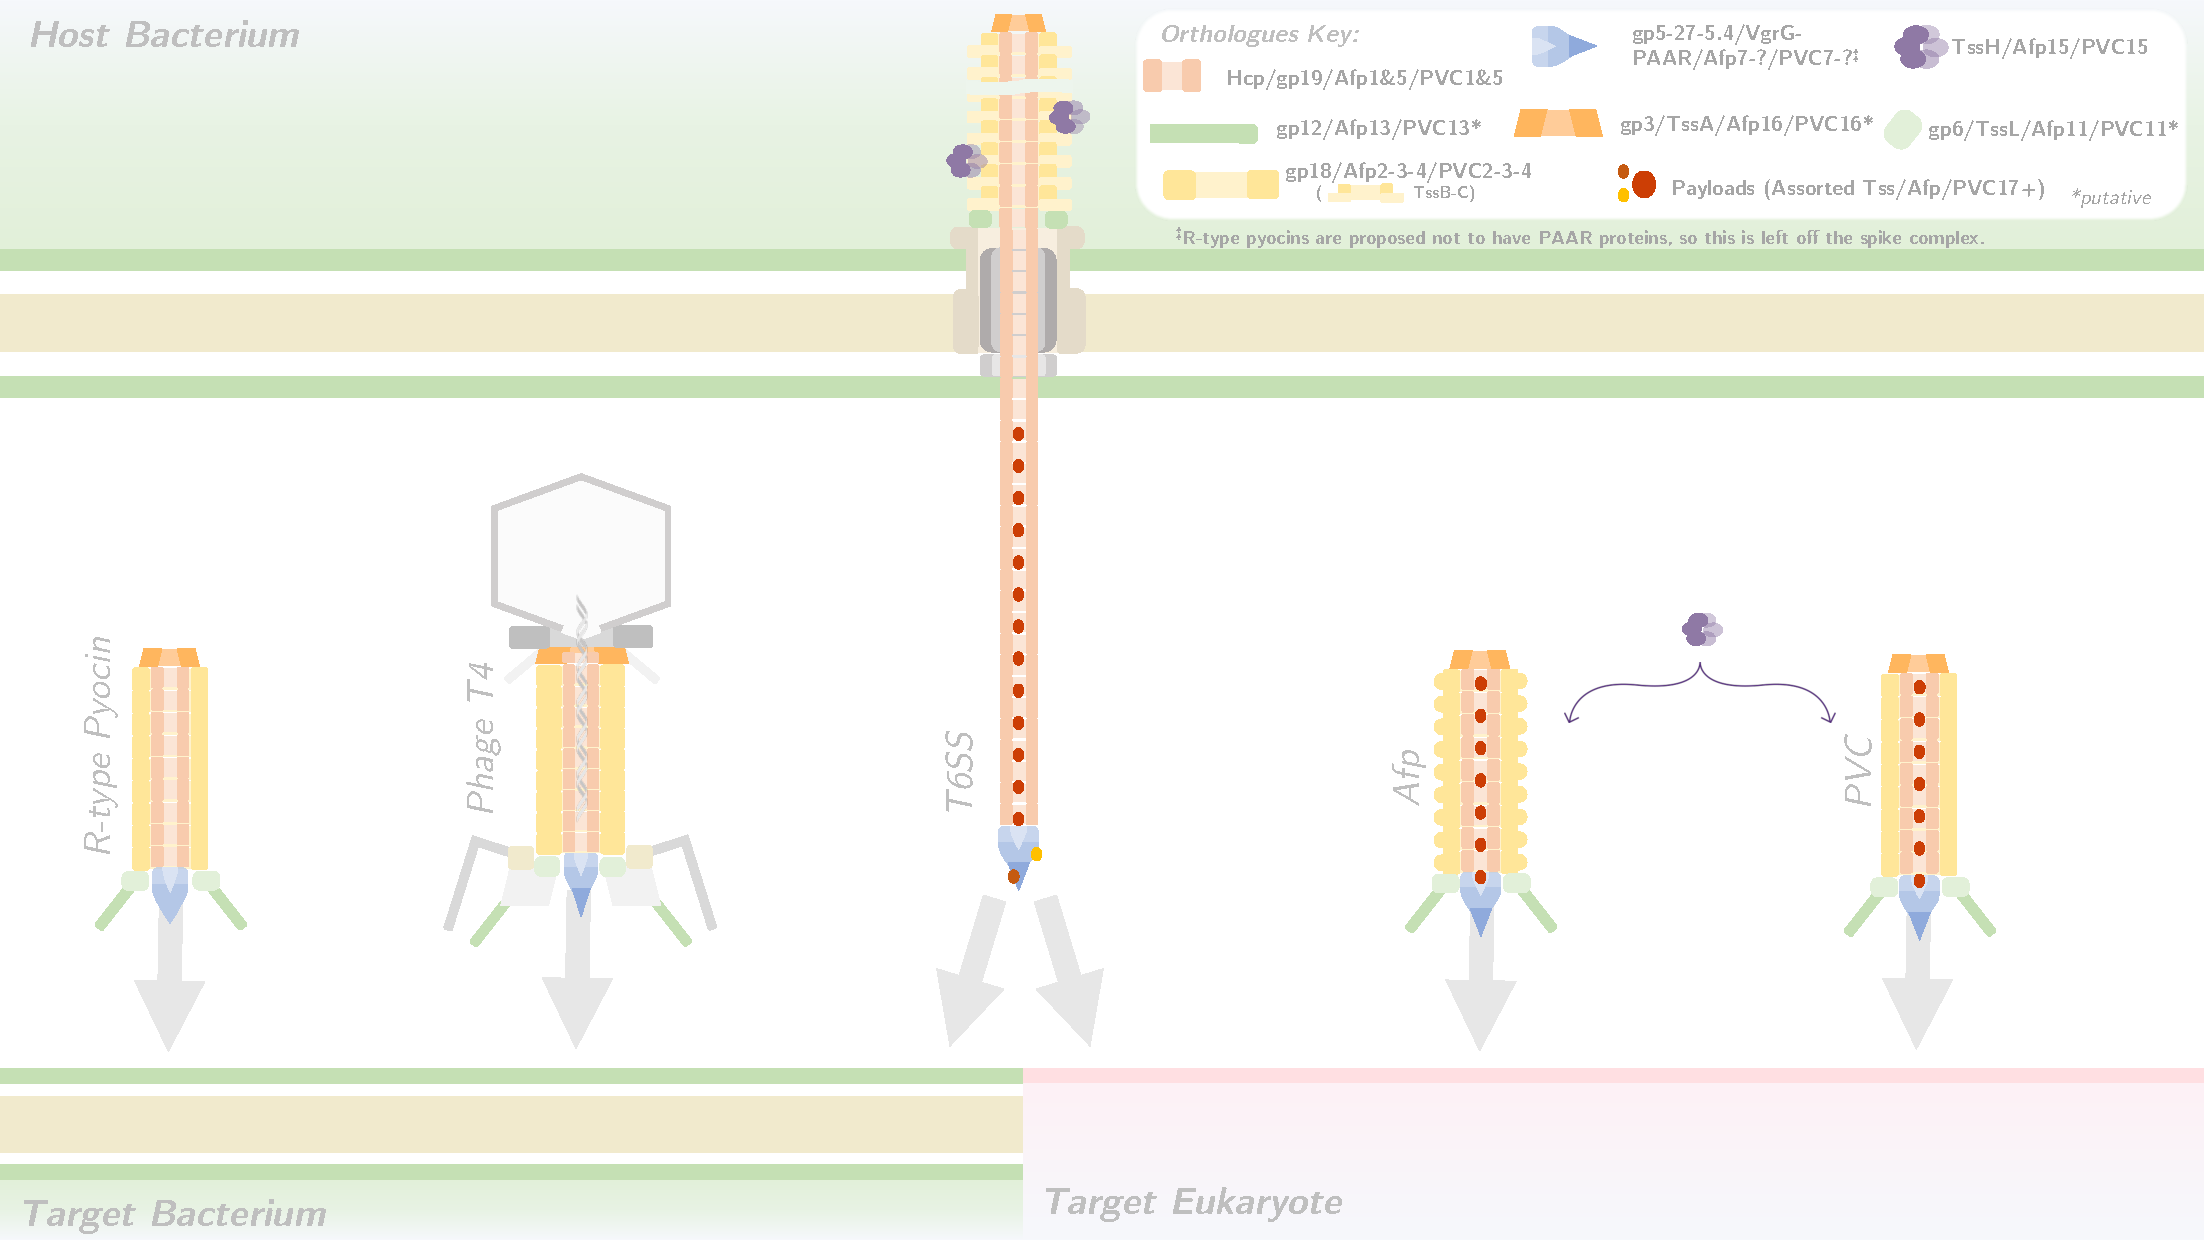
\includegraphics[width=\linewidth]{/Users/joehealey/Documents/Warwick/PhD/Thesis/chapters/intro/img/Structure_Comparison.pdf}
	\captionsetup{singlelinecheck=off, justification=justified, font=footnotesize, aboveskip=5pt}
	\caption[Schematic of conserved caudate architecture]{\textsc{\normalsize Schematic of conserved architecture in various caudate structures.}\vspace{0.1cm} \newline A diagrammatic comparison between the conserved components of PVCs and other caudate structures discussed in this introduction. The inset key depicts structural orthologs, though they may not be ancestrally related. Neutral/gray colours identify proteins which are not shared between structures. Items in the key with asterisks are putative homologues. A question mark indicates that a homologous structure has been identified, but the protein is not yet known. Not to scale.}
	\label{structure_diagram}
\end{figure}
\end{landscape}
\newpage

\subsection{Mechanism of Action}\label{mechanismofaction}
The actual mechanism of contraction has been the subject of significant debate and speculation in recent years. It has been generally accepted that the pre-contraction state of the tube complex represents an energetically tensioned system (meaning that the often seen of references to this conformation as `relaxed', is in fact, the exact opposite), and the prevailing hypothesis has been that the conformational change in the outer sheath proceeds in a wave-like fashion from the proximal baseplate, toward the capsid, and is driven by solvation free energy gain \citep{Brackmann2017, Kube2015a, Kube2014, Moody1973}. 

As the pre-contraction state is therefore an energetically unfavourable conformation, it begs the question of how contractile tail structures are able to be assembled seemingly against the laws of thermodynamics. While there is still no definitive answer to this, despite the wealth of data now available, the generally accepted mechanism is that the baseplate is produced first, in a static form (not changing in the contraction process), and serves as a `nucleation site' and a sort of intrinsic chaperone, allowing the first tier of the tube to polymerise off it. In effect, the baseplate is analogous to the pin in a mousetrap or a grenade, holding the conformation of the first tier in its a `locked' and tensioned state. The logic then follows that the tensioned tier 1 of the tube acts as an `auto-chaperone' allowing further tensioned forms of the tube hexamers (or dodecamers in the case of T6SS) to polymerise off it, also in a tensioned form \citep{Kube2015}.

For the T4 phage, it is now understood that the contraction of the tube is triggered by conformational changes transduced through the tail fibres, leading to large scale rearrangements in the baseplate. A contractile trigger mechanism for the Type 6 remains to be discovered, though the cryptic `antennae' that can be seen in the right panel of \vref{t6ssEMs}, may suggest that the T6SS is prompted to contract in a similar manner, which would also allow the cell to sense when a target is in close proximity, such that the T6SS is not discharged aberrantly, causing significant cost to the cell to regenerate. 

The contraction process is an enormously energetic process as a result of the release of the sheath tension. Not only is there a lateral translocation of the inner tube to provide the eversion, but the helical nature of the outer sheaths also applies a rotational torque to the sheath, quite literally drilling it in to the target cell envelope \citep{Kube2015}. This leads to some very impressive statistics. \cite{Wang2017} calculate that for contraction of a ``1 \um{} long sheath, composed of 260 rings, [the sheath] would push the inner tube by 420 nm and rotate it by 4.2 turns [...]. The overall amount of energy released during a single sheath contraction could be close to 44,000 kcal mol$^{-1}$". \cite{Vettiger2017} report that the entire contraction of the sheath occurs in just a couple of frames, even at 500 frames per second, and they conclude that the contraction speed is therefore \textgreater 800 nm per millisecond. The Type VI is  something of a special case given the lack of restriction on tube length, but \cite{Wang2017} calculate, on a per-subunit basis, that ``the free energy gained during contraction is 28.5 kcal mol$^{-1}$ subunit$^{-1}$, more than 9.1 kcal mol$^{-1}$ subunit$^{-1}$ calculated for [the] R-type pyocin". Exact contraction kinetics have not been observed for the other contractile mechanisms, but even the extrapolation here demonstrates that a significant amount of energy is expended by contractile machines to traverse these membranes \citep{Brackmann2017}.


\subsection{The \emph{status quo} of PVC genetics}
With the superficial resemblances to analogous structures covered, this section will briefly highlight the state of knowledge about the gene modules within the PVCs specifically when this project began. This provides the `jumping off point' for the upcoming Chapter, where the roles for many of these genes were probed further bioinformatically.

\subsubsection{The PVC tail tube and sheath}
As mentioned in previous sections, the tube and sheath components of the PVCs have long been among the best annotated genes within the operons, though this does not necessarily say much. Typical annotations, for instance from the first annotation of the published \emph{P. asymbiotica} ATCC43949 genome, for the ``LopT" PVC operon include ``phage tail sheath" and ``phage tail region" proteins. Belying the diversity of the PVCs which this thesis will continue to unpick, however, many of the operons still only picked up ``conserved hypothetical protein" annotations, even for these proteins. Of some approximately 350 CDSs made up from 16 operons identified in 3 genomes (see \vref{pvcvariants}), around 250 of them had no functional information whatsoever, and those that did were almost exclusively the cognate toxins and some tube proteins. Furthermore, in the TT01 genome, every single locus for every single PVC operon had the descriptor ``hypothetical protein", with no useful functional annotations whatsoever.

Nevertheless, with further inspection via BLAST and other tools, a good understanding of much of the PVC structure was able to be elucidated by \cite{Yang2006}. The phage tail tube proteins were unambiguously identified, though this wasn't true for the whole operon. Some additional observations could be made, including the deletion of a sheath protein in 3 operons. This raises questions about why the PVCs maintain 2 inner sheath and up to 3 outer sheath proteins, when at least one is evidently non-essential (assuming all PVCs are fully functional), and other caudate structures typically do not.

\subsubsection{The spike complex and baseplate}
The original genome annotations tell a similar story for the putative baseplate complex. What has subsequently been identified as the PVC's VgrG spike protein homologue, has only previously been annotated as hypothetical. Other structural components of a putative baseplate were detected however, with several operons displaying annotations for ``phage baseplate assembly proteins", ``similar to baseplate protein gp25". Though once again, the underlying variability in the PVCs means that a number of operons were left with uninformative annotations still. It is likely that much of the `dark matter' in the middle of the operon contributes to the baseplate apparatus, but with little to no orthology to anything previously detected in the databases.

\subsubsection{The operon core}
What is being termed here as the `operon core' describes a number of single copy genes located in the centre of the operon, which appear relatively conserved, and potentially have important non-structural roles. Though there are only a couple of useful annotations for this region, the \cite{Yang2006} paper was able to identify some compelling orthologues. Firstly, a gene which putatively has a role in transcript regulation resides in approximately locus position 10 (though this varies if operons have deleted upstream genes of course), but little else is known of its role, and the sequence identities are low \citep{Waterfield2009}. Immediately downstream of this is an unknown protein, with no functional information whatsoever.

The next gene, typically in locus position 13, is the putative tail fibre gene for the PVC complex. In the PVClumT operon of strain ATCC43949, this was attributed adenoviral tail fibre orthology. This is unusual, given the hypothesised bacteriophage origin of the structure, and there are no other known examples of this non-phage-like sequence similarity in other caudate structures, making the PVCs potentially unique. It has been demonstrated experimentally that the PVCs only exert toxic effects against eukaryotic targets (insect haemocytes), and have no antimicrobial activity whatsoever. It is possible that the reason for this that the PVCs have evolved anti-eukaryotic target recognition tail fibres, and thus they no longer bind to/work against prokaryotic targets. These unusual tail fibres are explored much more extensively in \vref{tailfibres}.

Positions 14 and 16 in the operon core also elaborate proteins with no readily apparent functions. The best hypothesis for these proteins, based on the experimental data and synteny with the \emph{Serratia} Afp, from the Hurst et al. experiments, is that they are the PVC equivalents of tape measure proteins and some kind of tube terminator or cap \citep{Rybakova2013, Rybakova2015}. \vref{structbioinfo} speculates on these proteins a little further.

Lastly, locus 15, despite not being well annotated in the originally available genomes, is readily identifiable as a AAA+ ATPase, like that of the T6SS (though from a distinct phylogenetic family \citep{Frickey2004}). Despite its ease of identification, there is currently no further experimental information available to suggest a role as covered in section \vref{t6ss}. The main hypothesis to date had been that the ATPase maybe served as a `loading pump', passing the PVC payloads in to the lumen of the tube, though this is purely speculation.

\subsubsection{The hypervariable payload region}
Finally, a hallmark of the PVCs which has been alluded to a few times in this introduction already, is the hypervariable toxin payload region. As there are multiple operons for each PVC, they each carry at least 1 unique toxic effector. This has not been observed with any other related structures, with the partial caveat of the fact that Type $x$ Secretion Systems are known to have various substrates, but they are not necessarily encoded \emph{cis} to the system itself. The carriage of \emph{cis} encoded toxins is true for the Afps as well, which once again highlights the similarity between them and PVCs. Similarly, while there are no shortage of caudate structures which have been identified in the literature, in studies like \cite{Sarris2014}, the PVCs remain unusual for this particular feature, and therefore potentially do not entirely fit in to the classifications others are attempting to apply to them.

The toxins encoded in the PVC loci are typically easy to identify, and have been reasonably well annotated, in part because they generally appear to be effectors which are already well known bacterial toxins from other systems. Pnf, for example, is and unequivocal orthologue of cnf1 from \emph{E. coli}, and was annotated as such in the original ATCC43949 genome. Similarly, the lopT operon in the same genome, harbours 3 different toxins, all of which have been seen in other instances. The lopT toxin itself takes its name from the yopT cysteine protease class of toxins in \emph{Yersinia}, an rtxA toxin is also present which is named for the family of toxins to which it belongs (``repeats-in-toxin"); a family that is well represented in other organisms, such as \emph{Vibrio} \citep{Lin1999}. Lastly, it also harbours a TccC domain protein, which are the toxic components of the Tc toxin complexes, which are actually elaborated by \emph{Photorhabdus} itself, separately, and were recently structurally resolved \citep{Bowen1998, Meusch2014} and are yet another staggeringly impressive toxin delivery mechanism of the bacteria. Nevertheless, following the trend in this section, not all operons were given useful or informative annotations, even for the toxins.


\subsection{PVC myths}
Despite the increasing wealth of information appearing, there are several papers which, in their attempts to group the PVCs with other structures, appear to come to spurious conclusions, and this section will briefly draw attention to these.

Firstly, \cite{Zhang2012a}, suggest that the ATPase which is distinctive within the PVCs has a role in cleavage/delivery of toxin molecules that is in some way separate from that of the PVC structure. There is little to no experimental evidence for this, and the majority of the paper disregards the actual syringe complex which is arguably the most important component. They do suggest that the ATPase may have a role in recycling the PVCs, as it has been shown to in the T6SS. However, as all the evidence to date points to the release of the PVCs, to act at a distance in a `torpedo' like fashion, there appears to be no evolutionary need/advantage to recycling the structure. That said, two possible explanations for its persistence, if recycling is its actual role, are that it may be vestigial, though this seems unlikely given the level of conservation. Given the fact that these ATPases are defined by their roles in various cellular pathways however, it could be that sufficient selection pressure to maintain the ATPases is being exerted based on their activity outside the PVC operons \citep{Iyer2004}. Alternatively, the ATPase may recycle the tube subunits continually so that they do not build up unnecessarily inside the cell, before mature PVCs are ready to be deployed `in anger'. Since so many more of these proteins are required per syringe, its possible that they're made in significantly higher proportions, and to offset the metabolic cost of building such a structure aberrantly, they are being turned over continually to replenish cellular concentrations of amino acids and other substrates.

They speculate that the N-termini of the toxin effector molecules contain a distinctive metallo-peptidase domain/activity, though the paper is not clear on what sequences were used to arrive at this conclusion. From our own studies (as yet unpublished), it has been demonstrated that the N-termini of the toxins for several PVC effectors have a stabilising/chaperone-like role, possibly with a syringe loading signal. However, it is more or less impossible to construct a meaningful multiple sequence alignment for all but the most closely related effectors, much less to define a characteristic domain structure for all PVC toxins, which calls in to question some of the conclusions of the paper, at least for the sequences they are attributing to PVCs.

Despite being an otherwise excellent review, Kube and Wendler make the statement that  PVC sheath proteins are most like T4 sheath proteins, but pyocin proteins are most like phage P2. This appears only partly true however \citep{Kube2015}. \vref{structbioinfo} examines this further, but it appears that actually only one of the sheaths (the inner) is T4 like, whereas the outer is pyocin- (and therefore P2) like, also resembling the T6SS. In the same paper, the authors also make the statement that the Afp cluster lacks any lysis systems, which are seen in phage and pyocins. While it is true that evidence for lysis-based release of the PVCs and Afps is scarce as the authors point out, the PVCs can often be found with lysis associated proteins. For example, downstream of the PVCPnf ATCC43949 operon, beyond the payload region, but on the same strand and in close register to the rest of the operon, several bacteriophage lysis proteins and lysozymes can be detected, though it is true that this cannot be said for all of the operons, at least at the present level of sequence identification. It seems the likely do harbour general lysis systems, though some of them may be comparatively enigmatic.

Similarly, though it is also an excellent study, the \cite{Sarris2014} paper makes many claims about the PVCs in attempting to group them with other ``Phage-Like-Translocation-Systems", though they appear to be only considering a single PVC example from \Plum{} (``Unit2"), and some of these statements may not hold true for all PVCs. One example of an erroneous claim is in their discussion of synteny conservation. While there is undoubtedly a great deal of synteny conservation, they state that the sheath proteins are typically located downstream of baseplate genes. It's not clear whether this is simply a syntactical or typographical error, but it's readily apparent, including from the figures in their own paper, that the reverse is true. Since they are basing a level of significance on these similarities for identifying similar structures elsewhere, this synteny rearrangement would potentially have consequences for how sequences are grouped and ancestry inferred. Another objectionable conclusion is their readiness to include many, potentially distantly related, operons in to this ``PLTS" family, without any actual consideration being paid to whether the operons harboured any payloads which are translocatable. This is important, as they identify R-type pyocins, which are non-translocating structures, as a separate `clade'. Thus, whether or not a candidate caudate structure should be considered more like an R-type pyocin or an Afp/PVC cannot be decided from sequence alone due to the huge diversity, and functional relatedness is therefore a key factor. Additionally, Sarris and colleagues also fall foul of the same observation as \cite{Kube2015}, in stating that there are no lysis proteins associated with PVCs. Had they considered more than one PVC example in their analysis, they may have observed that this doesn't appear to be true.

\section{Summary and Thesis Aims}
Despite this richness of data for related systems - the cumulative product of centuries of study - the picture is, perhaps unsurprisingly, still far from complete for the PVCs, being comparatively understudied. Their unique role as bacterial secretion systems that act at a distance means there is much left to be understood about what makes them different. This thesis attempts to tackle this in a number of ways:

\begin{itemize}
\item Firstly, an up-to-date exploration of the structural similarities and differences with the benefit of time and more advanced bioinformatics resources/databases versus the original description of PVCs can be found in \vref{structbioinfo}. This chapter aims to improve understanding of the poorly characterised genes for all the proteins in the operons, and generate hypotheses for testing in the lab and for future work.

\item Secondly, a phylogenetic study of the PVCs which attempts to shed light on the microevolution within the operons, examining the variability and loss of genes in this context, can be found in \vref{bioinformatics}. All the comparative genomic studies that have been covered in this introduction are keen to place the PVCs in a wider context, whereas an inward-looking study trying to better understand why so many PVC variants exist, and why they are so diverse has been lacking. 

\item Key proteins in the mechanistics of (at least) non-membrane-bound caudate structures are the tail fibres. They are responsible for triggering the contractile mechanisms, and also conferring the `target spectrum' that the structures are able to act against. For the PVCs, sequence similarities in these proteins were weak at the outset, though curiously, some were able to pick up annotations against Adenoviral motifs. \vref{tailfibres} explores the tail fibres in more detail, and represents possibly the first experimental studies of naturally occurring chimeric tail fibres.

\item \vref{regulation} explores efforts to understand the natural expression patterns of the PVCs, as well as attempts to heterologously clone and express the PVC operons. Experimental work to date had been conducted with a cosmid library, but there were several issues with this approach. The PVCs were still under the control of their native promoters, and this made them unstable and difficult to work with in the lab. A key question for this chapter, therefore, is to try and probe any population heterogeneity in how the PVCs are deployed naturally.

\end{itemize}



\newpage

%%%%%%%%%%%%%%%%%%%%%%%%%%%%%%%%%%%%%%%%%%%%%%%%%%%%%%%%%%%%%%%%%%%%%%%%
%%                                                                    %%
%%                      IMPORT CH2 - METHODS                          %%
%%                                                                    %%
%%%%%%%%%%%%%%%%%%%%%%%%%%%%%%%%%%%%%%%%%%%%%%%%%%%%%%%%%%%%%%%%%%%%%%%%
\pagestyle{IHA-fancy-style}
\lhead{\textsf{Chapter II}}
\rhead{\textsf{Materials \& Methodology}}


\chapter{Materials \& Methodology}\label{methods}

All methods from all chapters are collected here in detail, for clarity. Where appropriate, the methods have been reiterated at a higher level, in the context of the experimental workflow in their respective chapters.

%\section{Materials Suppliers}
%Unless indicated otherwise, materials were procured from the following manufacturers:
%
%\small
%\begin{itemize}
%\item \emph{PCR enzymes}: Invitrogen \emph{Taq} was purchased from ThermoFisher Scientific. Q5\textsuperscript{\textregistered} Polymerase was purchased from New England Biolabs (NEB).
%\item \emph{Restriction Enzymes}: All restriction enzymes were purchased from New England Biolabs
%\item \emph{Strains}: Most strains used in this study were provided by other labs, but those that were purchased came from New England Biolabs.
%\item \emph{Oligonucleotides}: Primers and synthesised oligonucleotides were primarily purchased from Integrated DNA Technologies (IDT) or Sigma-Aldrich
%\item \emph{Protein Purification Columns}: Gel filtration and IMAC columns were purchased from General Electric (GE) Healthcare
%\item \emph{Media}: Most media is provided pre-made at the University of Warwick. Autoinduction Media is a Formedium product.
%\end{itemize}
%
%
%\normalsize


\section{Bacterial Culture Techniques}
The vast majority of this project, as a molecular and synthetic biology research project,  involved microbial culture and heterologous expression work. Despite being a thesis on the study of \Pa, almost all of the work conducted was in \emph{E. coli}. As a member of the \emph{Enterobacteriaceae}, \Pa{} is fairly closely related to \emph{E. coli}, thus much of the genetic work can be conducted in the considerably more tractable lab strain with few, if any, complications.

\subsection{Strains}
A number of specialist and host strains were used for various purposes and they are detailed in \vref{strains}, along with their purpose, and if available, their genotypes. With the exception of BL21(DE3) ``NiCo21"'s, which were purchased from New England Biolabs, and DY380 which was a gift from Donald Court\footnote{\url{https://redrecombineering.ncifcrf.gov/}}, all strains were present in the lab freezer stocks. Their original sources are provided in the table.

\begin{landscape}
\scriptsize
\captionsetup{singlelinecheck=off, justification=justified, font=footnotesize}
\rowcolors{1}{gray!10}{white}
\begin{tabularx}{\linewidth}{>{\centering\arraybackslash}m{0.07\linewidth}  >{\raggedright\arraybackslash}m{0.415\linewidth} >{\raggedright\arraybackslash}m{0.32\linewidth}  >{\centering\arraybackslash}m{0.14\linewidth}}
\hiderowcolors
\caption[Strains]{\emph{E. coli} strains used throughout this work, their available genotypic data, and their originating source.}
\label{strains}\\

Strain  & Genotype & Purpose & Reference\\[0.5ex]
\hline\hline
\multicolumn{4}{p{\linewidth}}{\centering Cloning/Plasmid Maintenance Strains}\tstrut\bstrut \\
\hline
\showrowcolors
DH5-$\alpha$ & F- \emph{endA1 glnV44 thi-1 recA1 relA1 gyrA96 deoR nupG purB20 $\phi$80dlacZ$\Delta$M15 $\Delta$(lacZYA-argF)U169, hsdR17(rK-mK+), $\lambda$-} \newline HB1100 derivatised strain from Bethesda Research Laboratories
& High transformation efficiency general purpose cloning strain. Cloning and plasmid maintenance & \citep{Glover1995} \\

DH10-$\beta$ (``TOP10") & F- \emph{endA1 deoR+ recA1 galE15 galK16 nupG rpsL $\Delta$(lac)X74 $\phi$80lacZ$\Delta$M15 araD139 $\Delta$(ara,leu)7697 mcrA $\Delta$(mrr-hsdRMS-mcrBC) StrR $\lambda$-} \newline MC1061 derivatised strain & High transformation efficiency general purpose cloning strain, reported to be more tolerant of large inserts/constructs. Maintenance of cosmids and large constructs & Invitrogen \\

EC100 & F- \emph{mcrA $\Delta$(mrr-hsdRMS-mcrBC) $\phi$80dlacZ$\Delta$M15 $\Delta$lacX74 recA1 endA1 araD139$\Delta$(ara, leu)7697 galU galK $\lambda$- rpsL nupG}  & High transformation efficiency cloning strain for exceptionally large constructs (cosmids/BACs etc.) Used in this study to harbour cosmid library & Epicenter (Lucigen) \\

S17$\lambda$\emph{pir} & \emph{TpR SmR recA, thi, pro, hsdR-M+RP4: 2-Tc:Mu: Km Tn7 $\lambda$pir}  & \Ec{} strain for maintenance of conjugable plasmids & Biomedal \\


\hline
\multicolumn{4}{p{\linewidth}}{\centering Expression Strains}\tstrut\bstrut \\
\hline

\hiderowcolors
NEB ``NiCo21" BL21(DE3) & \emph{can::CBD fhuA2 [lon] ompT gal ($\lambda$ DE3) [dcm] arnA::CBD slyD::CBD glmS6Ala $\Delta$hsdS $\lambda$ DE3 = $\lambda$ sBamHIo $\Delta$EcoRI-B int::(lacI::PlacUV5::T7 gene1) i21 $\Delta$ nin5} \newline Derivatised BL21(DE3) with reduced proteases/IMAC contaminating proteins & IMAC optimised BL21 expression strain lysogenised with the DE3 prophage for T7-polymerase driven expression via IPTG induction & New England Biolabs \\
\showrowcolors


\hline
\multicolumn{4}{p{\linewidth}}{\centering Recombineering Strains}\tstrut\bstrut \\
\hline


DY380 & F- \emph{mcrA $\lambda$(mrr-hsdRMS-mcrBC) $\phi$80dlacZ M15 $\Delta$lacX74 deoR recA1 endA1 araD139 $\Delta$(ara, leu) 7649 galU galK rspL nupG [ $\lambda$cI857 (cro-bioA) $<>$ tet]} \newline Derivatised DH10-$\beta$ strain with defective $\lambda$ prophage and temperature sensitive cI875 repressor  & Recombineering strain with the $\beta$, $\gamma$ and $exo$ proteins chromosomally located. Can be derepressed by temperature shift to 42\degC. Used in this study to modify cosmids and overcome plasmid shortcomings. & \citep{Lee2001} \\

BW25113 & F- \emph{$\Delta$(araD-araB)567, lacZ4787($\Delta$)::rrnB-3, LAM-, rph-1, $\Delta$(rhaD-rhaB)568, hsdR514} \newline Derivative of K12 strain BD792 & Keio Collection WT Parent strain. A $\Delta$\emph{rfaH} strain was used in this study for regulation analysis experiments, and the wild type was retained as a control. & \citep{Baba2006} \\

\end{tabularx}
\end{landscape}
\newpage

\subsection{Culture Conditions}
	\subsubsection{Media}
		\paragraph{LB}
		Routine culture of \emph{E. coli} and \Pa{} was conducted in standard Lysogeny Broth (LB) liquid media and agar plates, at 200 RPM in a shaking incubator (or static incubator for plates). The media is supplemented with 0.1\% pyruvate when culturing \Pa. For \Plum{} strains, cultures were grown at 28\degC{} due to their temperature intolerance.
		\paragraph{SOC}
		Super Optimal Media with catabolite repression (SOC), is a high glucose medium routinely used in the recovery culture phase of bacterial transformation. It is designed to be a rich media which reduces stress on the transformed cells, allowing them to optimally uptake the target DNA. In particular, the high glucose content in comparison to standard LB media is useful as it represses the pBAD promotor system (used quite extensively in this study - see \vref{plasmids}), helping to clone otherwise potentially toxic/recalcitrant targets.

	\subsubsection{Antibiotics \& Media Supplements}\label{Antibiotics}
	Various antibiotics and media supplements were used during this project. \vref{supplementtable} shows concentrations of compounds used.
	
	
\begin{table}[H]
\scriptsize
\captionsetup{singlelinecheck=off, justification=justified, font=footnotesize}
\caption[Media Supplements]{Antibiotics and other media supplements, and the final concentrations for use.}
\begin{tabularx}{0.7\textwidth}{ c c }
Supplement & Working Concentration  \\[0.5ex]
\hline\hline
\multicolumn{2}{p{0.5\textwidth}}{\centering Antibiotics}\tstrut\bstrut \\
\hline
Ampicillin & 100 \ugml \\
Kanamycin & 25 \ugml \\
Chloramphenicol & 25 \ugml \\
Gentamycin & 10 \ugml \\
Tetracycline & 10 \ugml \\
\hline
\multicolumn{2}{p{0.5\textwidth}}{\centering Growth Supplements}\tstrut\bstrut \\
\hline

Pyruvate & 0.1 \% (w/v) \\
\hline
\multicolumn{2}{p{0.5\textwidth}}{\centering Expression}\tstrut\bstrut \\
\hline

Arabinose & 0.2\% (w/v) \\
IPTG & 2 mM \\
Tetracyline & 0.2 $\mu$M \\
\hline
\multicolumn{2}{p{0.5\textwidth}}{\centering Repression}\tstrut\bstrut \\
\hline
Glucose & 0.2\% (w/v) \\

\label{supplementtable}
\end{tabularx}
\end{table}



		
\section{Molecular Techniques - Nucleic Acid Methods}

\subsection{Purification of Nucleic Acids}
	DNA isolation was a frequent task in the course of this work. Replicon DNA in the form of plasmids and cosmids was required for screening, cloning and expression purposes. Genomic DNA was purified for PCR templates and for assessment of recombination. This was performed exclusively via commercial kit. Manufacturers protocols were followed in every case, with some minor modifications, which are detailed in this section. In all cases, DNA once purified was stored at -20\degC.
	
	\subsubsection{Genomic DNA}\label{gdna}
		Genomic DNA (gDNA) is isolated with the Qiagen ``Blood and Tissue" extraction kit, with the following modifications for bacterial culture:

		 5 - 10 mL of overnight culture is set up in appropriate conditions (i.e. with selection if possible). Cells are pelleted at 7,000 RCF, 4\degC{} for 10 minutes. Pellets are resuspended in 180\ul{} of the manufacturer supplied ATL buffer, with 20\ul{} of the supplied Proteinase K mix added. RNAse H is optionally added if the DNA is to be used for next generation sequencing. From here the protocol proceeds directly to the manufacturers step 2, and follows the standard procedure until elution. Elution was conducted in 2 x 17.5\ul{} washes in AE buffer (unless it is to be used for sequencing, then H$_2$O or EB Buffer is used).

	\subsubsection{Replicon DNA}
			\paragraph{Plasmids}\label{Plasmids}
		For plasmid isolation the Qiagen Miniprep Spin Kit was used according to the manufacturers instructions. 5 - 10 mL overnights of culture are prepared in appropriate conditions (e.g. for plasmids with selection, add antibiotics - see \vref{Antibiotics}). 10 mL of culture is used for lower copy number plasmids, to ensure adequate DNA recovery. Elution was conducted in 2 x 17.5 \ul{} washes, with molecular grade water instead of a single 50 \ul{} buffer wash. For isolation of cosmids, and plasmids in excess of $\approx$ 10 kbp, the same miniprep kit is used, but with the manufacturers suggested optional optimisations, namely: the optional wash with PB buffer is conducted, and elution buffer/water is preheated to 70\degC. 2 x 17.5 \ul{} washes are conducted as in plasmid preparation.

\newpage
	\subsection{Plasmids and Cosmids}
	All plasmids were either bought, gifted or created in this study. Recombineering plasmids pKD46/pCP20/pJET-FRT-Cm/pJET-FRT-Kan were a kind gift from Dr. Helge Bode at Goethe University, Frankfurt. pET29a was received from Jenny Goodman, a fellow PhD student at Warwick.
	
	\vref{plasmidtable} details all the existing plasmids used in this study that have been previously constructed and/or published. \vref{customplasmids} details all the constructs produced during the course of this study. 
	
\begin{landscape}
\scriptsize
\captionsetup{singlelinecheck=off, justification=justified, font=footnotesize}
\rowcolors{1}{gray!10}{white}
\begin{tabularx}{\linewidth}{ >{\centering\arraybackslash}m{0.13\linewidth} >{\raggedright\arraybackslash} m{0.68\linewidth} >{\raggedleft\arraybackslash} m{0.16\linewidth} }
\hiderowcolors
\caption[Plasmids]{Existing plasmids used as the bases for derivations listed in \vref{customplasmids}. All plasmids were either gifted, existed in lab stocks already, or purchased.}
\label{plasmidtable}\\

Plasmid Designation  & Purpose &  Reference\\[0.5ex]
\hline\hline
\multicolumn{3}{p{\linewidth}}{\centering Cloning/Expression Plasmid Bases}\tstrut\bstrut \\
\hline
\showrowcolors
pBAD30 & Basic inducible expression vector. Arabinose inducible via \emph{araBAD} system, glucose repressible. Ampicillin resistant, with a p15 \emph{ori} (compatibility group B) and f1 \emph{ori} (compatibility group A). & \citep{Guzman1995} \\

pET15b & Inducible expression vector. IPTG inducible via \emph{lac}/T7 polymerase system, glucose repressible. Ampicillin resistant, with ColE1 \emph{ori} (compatibility group A). The plasmid contains an N-terminal hexa-histidine tag with a thrombin cleavage site for in-frame tagging of recombinant protein and cleavage after purification. & Novagen \\

pET29a & Inducible expression vector. IPTG inducible via \emph{lac}/T7 polymerase system, glucose repressible. Kanamycin resistant, with ColE1 \emph{ori} (compatibility group A). The plasmid contains a C-terminal hexa-histidine tag with a thrombin cleavage site for in-frame tagging of recombinant protein and cleavage after purification. Additionally contains an N-terminal Streptavidin tag. & Novagen \\

pGAG1 & Promoterless GFP reporter `empty' vector. Conjugative plasmid requiring $\lambda$\emph{pir} \emph{E. coli} for propagation. & CITATION NEEDED \\

pAGAG & Promoterless GFP bearing plasmid, without GFP start codon for promotor fusion reporter construct creation. Conjugative plasmid requiring $\lambda$\emph{pir} \emph{E. coli} for propagation. & CITATION NEEDED \\

\hline
\hiderowcolors
\multicolumn{3}{p{\linewidth}}{\centering Recombineering Plasmids}\tstrut\bstrut \\
\hline
\showrowcolors

pKD46 & $\lambda$Red plasmid bearing $\beta$, $\gamma$, and \emph{Exo} recombineering enzymes, under the arabinose inducible control of the \emph{araBAD} system. Ampicillin resistant, with the temperature sensitive \emph{ori} 101ts (compatibility group C) & \citep{Datsenko2000} \\

pCP20 & FRT ``flippase" bearing plasmid for excision of regions surrounded by FRT recognition sites (typically after successful recombineering with pKD). Ampicillin and Chloramphenicol resistant, with the temperature sensitive \emph{ori} 101ts (compatibility group C). & \citep{Datsenko2000} \\

pJET-FRT-Cm & Recombineering knockout cassette template plasmids bearing an FRT-flanked Chloramphenicol cassette. Ampicillin and Chloramphenicol resistant, with a ColE1 \emph{ori} (compatibility group A). & Helge Bode (derivatised Thermo Scientific Vector)\\

pJET-FRT-Kan & Recombineering knockout cassette template plasmids bearing an FRT-flanked Kanamycin cassette. Ampicillin and Kanamycin resistant, with a ColE1 \emph{ori} (compatibility group A). & Helge Bode (derivatised Thermo Scientific Vector) \\

\end{tabularx}

\newpage
%%%%%%%%%%%%%%%%%%%%%%%%%%%%%%%%%%%%%%%%%%%%%%%%%%%%%%%

\captionsetup{singlelinecheck=off, justification=justified, font=footnotesize}
\rowcolors{1}{gray!10}{white}
\begin{tabularx}{\linewidth}{ c >{\centering\arraybackslash} m{0.26\linewidth} >{\centering} m{0.08\linewidth} m{0.48\linewidth} }
\hiderowcolors
\caption[Custom Plasmids]{Cloned and/or derivatised plasmids created during the course of this study.}
\label{customplasmids}\\

Plasmid Designation & Insert & Backbone  & Function/Purpose\\[0.5ex]
\hline\hline
\multicolumn{4}{p{\linewidth}}{\centering Expression Constructs}\tstrut\bstrut \\
\hline
\showrowcolors

pET15b\_\emph{pnf13} & PVC\emph{pnf} Putative Tail Fibre Gene & pET15b & PVC\emph{pnf13} Tail fibre cloned in-frame with the N-terminal hexa-histidine tag and thrombin cleavage site, for expression and purification via IMAC \\

pET15b\_\emph{lumt13} & PVC\emph{lumt} Putative Tail Fibre Gene & pET15b & PVC\emph{lumt13} Tail fibre cloned in-frame with the N-terminal hexa-histidine tag and thrombin cleavage site, for expression and purification via IMAC \\

pET29a\_\emph{pnf13} & PVC\emph{pnf} Putative Tail Fibre Gene & pET29a & PVC\emph{pnf13} Tail fibre cloned in-frame with the C-terminal hexa-histidine tag and thrombin cleavage site, for expression and purification via IMAC \\

pET29a\_\emph{lumt13} & PVC\emph{lumt} Putative Tail Fibre Gene & pET29a & PVC\emph{lumt13} Tail fibre cloned in-frame with the C-terminal hexa-histidine tag and thrombin cleavage site, for expression and purification via IMAC \\

\hline
\multicolumn{4}{p{\linewidth}}{\centering Reporter Constructs}\tstrut\bstrut \\
\hline

pAGAG\_PB68.1PVCpnf & \emph{P. asymbiotica} Thai PB68.1 PVC\emph{pnf} promoter & pAGAG & \emph{P. asymbiotica} strain Thai PB68.1 PVC\emph{pnf} operon promoter fused to GFP\\

pAGAG\_PB68.1PVClopT & \emph{P. asymbiotica} Thai PB68.1 PVC\emph{lopT} promoter & pAGAG & \emph{P. asymbiotica} strain Thai PB68.1 PVC\emph{lopT} operon promoter fused to GFP\\

pAGAG\_PB68.1PVCcif & \emph{P. asymbiotica} Thai PB68.1 PVC\emph{cif} promoter & pAGAG & \emph{P. asymbiotica} strain Thai PB68.1 PVC\emph{cif} operon promoter fused to GFP\\

pAGAG\_PB68.1PVCU1 & \emph{P. asymbiotica} Thai PB68.1 PVC\emph{Unit1} promoter & pAGAG & \emph{P. asymbiotica} strain Thai PB68.1 PVC\emph{Unit1} operon promoter fused to GFP\\

pAGAG\_TT01PVCU4 & \emph{P. luminescens} TT01 PVC\emph{Unit4} promoter & pAGAG & \emph{P. luminescens} strain TT01 PVC\emph{pnf} operon promoter fused to GFP\\

pAGAG\_TT01PVClopT & \emph{P. luminescens} TT01 PVC\emph{lopT} promoter & pAGAG & \emph{P. luminescens} strain TT01 PVC\emph{pnf} operon promoter fused to GFP\\

pAGAG\_TT01PVCcif & \emph{P. luminescens} TT01 PVC\emph{cif} promoter & pAGAG & \emph{P. luminescens} strain TT01 PVC\emph{pnf} operon promoter fused to GFP\\

pAGAG\_TT01PVCU1 & \emph{P. luminescens} TT01 PVC\emph{Unit1} promoter & pAGAG & \emph{P. luminescens} strain TT01 PVC\emph{pnf} operon promoter fused to GFP\\

\end{tabularx}

\end{landscape}

\subsection{PCR}
	\subsubsection{Primers}\label{primers}
	All primers used in this study were purchased from Integrated DNA Technologies (IDT).

\begin{table}[H]
\scriptsize
\captionsetup{singlelinecheck=off, justification=justified, font=footnotesize}
\caption[Primer Sequences]{Primer sequences used in this study for simple amplification and detection purposes - no sequence modifications. Annealing temperatures are given as per the IDT Oligoanalyzer's reported value, or, in the case of values in square parentheses, those given by NEB Tm Calculator (with 500 nM primer concentration and Q5 product group parameters).}
\vspace{0.2cm}
\begin{tabularx}{\linewidth}{ c c L  c  c }

Primer Name  & Function & \multicolumn{1}{c }{Sequence (5' $\rightarrow$ 3')} & Tm ($^{\circ}\mathrm{C}$) & Length (bp)\\[0.5ex]
\hline\hline
no1\_F & \multirow{2}{*}{Detection of pJET} & CGCACTTCCAGACCCAGATC & 57.9 & \multirow{2}{*}{$\approx$1200}\\[0.5ex]
no2\_R & &  GATGGAGTAAATGGTACCTTGGG & 55.1 & \\[0.5ex]

Gam\_Bet\_F & \multirow{2}{*}{Detection of pKD/pCP} & TTTCACAGCTATTTCAGGAGTTC & 52.9 & \multirow{2}{*}{1112}\\[0.5ex]
Gam\_Bet\_R & &  CATGCTGCCACCTTCTG & 53.8 & \\[0.5ex]

T7\_Prom\_F & \multirow{2}{*}{T7 Sequencing Primer} & TAATACGACTCACTATAGGG & 46.5 [58] & \multirow{2}{*}{Varied}\\[0.5ex]
T7\_Term\_R & &  GCTAGTTATTGCTCAGCGG & 46.5 [58] & \\[0.5ex]

rfaH\_5'\_SP\_F & \multirow{2}{*}{rfaH Knockout Sequencing Primer} & CAACTTCACGCAGCG & 51.4 [62] & \multirow{2}{*}{Varied}\\[0.5ex]
rfaH\_3'\_SP\_R & & TATGACATTGCTGGAGCC & 52.2 [62] & \\[0.5ex]


\label{primertable}
\end{tabularx}
\end{table}
\todo[inline]{Finish populating all primer tables}

\begin{landscape}
\scriptsize
\captionsetup{singlelinecheck=off, justification=justified, font=footnotesize}


\begin{tabularx}{\linewidth}{c  c  L c  c }
\caption[Functionalised Primer Sequences]{Primers for specialist purposes, harbouring modifications, including restriction sites for cloning and overlap homologies for recombineering and Gibson Assembly. Restriction Sites are shown in \textbf{bold}. Overlap homology is shown \underline{underlined} Annealing temperatures shown in [ ] are specific to NEB's Q5 Polymerase. F: Forward Primer, R: Reverse Primer, bp - Base Pair.}
\label{specprimers}\\

Primer Name  & Function/Target  & \multicolumn{1}{c}{Sequence (5' $\rightarrow$ 3')} & Tm ($^{\circ}\mathrm{C}$) & Length (bp)\\
\hline\hline
\multicolumn{5}{p{\linewidth}}{\centering Classical Cloning}\tstrut\bstrut\\
\hline\tstrut\bstrut

PVCpnf13-NdeI\_F & \multirow{3}{*}{\emph{pnf} Tail Fibre} & GAGTTA\textbf{CATATG}AACGAAACTCGTTATAATGC & [67] & \multirow{3}{*}{1548} \\
PVCpnf13-BamHI\_R & & TTTTCA\textbf{GGATCC}TTAAAGCTTTATGATGAAAGC & [67] &  \\
PVCpnf13-KpnI\_R & & TTTTCA\textbf{GGTACC}AAAAGCTTTATGATGAAAGC & [67] & \\

PVClumt13-NdeI\_F & \multirow{3}{*}{\emph{lumt} Tail Fibre} & GCCGGA\textbf{CATATG}GACAACAAAAATAAC & [67] & \multirow{3}{*}{675} \\
PVClumt13-BamHI\_R & & TTACTT\textbf{GGATCC}TTACACAACCTTAATCATATAG & [67] &  \\
PVClumt13-KpnI\_R & & TTACTT\textbf{GGTACC}AACACAACCTTAATCATATAG & [67] & \\

%
rfaH\_EcoRI\_F & \multirow{2}{*}{\emph{rfaH}} & ACAGGT\textbf{CATATG}GAATTAAATGAGTTAACTAACAAATT & [71] & \multirow{2}{*}{500} \\
rfaH\_SalI\_R & & CTA\textbf{GTCGAC}TTAGAGTTTGCGGAACTCG & [71] & \\

\hline
%%%%%%%%%%%%%%%%%%%%%%%%%%%%%%%%%%%%%%%%%%%%%%%%%%%%%%%%%%%%%%%%%%%%%
\multicolumn{5}{p{\linewidth}}{\centering Gibson Assembly}\tstrut\bstrut \\
\hline\tstrut\bstrut
%%%%%%%%%%%%%%%%%%%%%%%%%%%%%%%%%%%%%%%%%%%%%%%%%%%%%%%%%%%%%%%%%%%%%

pBAD30frag\_F & \multirow{2}{*}{pBAD30} & \underline{ATGTAATTAATTCAACCATCACGGAGAGTTTATCA}ACGCCGTAGCGCCGATGGTAGTGTGGGGTCTCCCC & [72] & \multirow{2}{*}{4791} \\
pBAD30frag\_R & & \underline{CTTGTAGACATAAAAGCCCCTTTTTAGACAAAAAA}TAGCCCAAAAAAACGGGTATGGAGAAACAGTAGAG & [72] &  \\

PNFfrag1\_F & \multirow{2}{*}{PVC\emph{pnf} 1-8} & \underline{CTCTACTGTTTCTCCATACCCGTTTTTTTGGGCTA}TTTTTTGTCTAAAAAGGGGCTTTTATGTCTACAAG & [72] & \multirow{2}{*}{7181} \\
PNFfrag1\_R & & \underline{GTGTCAGTATTTGATTTTCCATTCATCGTCACCTT}TCATTGGGTAAGATTAATTTTTGCGCCTTTGATTT & [72] &  \\

PNFfrag2\_F & \multirow{2}{*}{PVC\emph{pnf} 9-12} & \underline{AAATCAAAGGCGCAAAAATTAATCTTACCCAATGA}AAGGTGACGATGAATGGAAAATCAAATACTGACAC & [72] & \multirow{2}{*}{6039} \\
PNFfrag2\_R & & \underline{TCTTGTACAGTTGCATTATAACGAGTTTCGTTCAT}GATTAACTCCAGAAAACATATTTAATTCAACATCA & [72] &  \\

PNFfrag3\_F & \multirow{2}{*}{PVC\emph{pnf} 13-15} & \underline{TGATGTTGAATTAAATATGTTTTCTGGAGTTAATC}ATGAACGAAACTCGTTATAATGCAACTGTACAAGA & [72] & \multirow{2}{*}{5514} \\
PNFfrag3\_R & & \underline{TTATTGACATCAATAATAGTTTGCGTGTTTAACAT}AAAAAACCTCTCTTAAATTATATCGTGATAACTTT & [72] &  \\

PNFfrag4\_F & \multirow{2}{*}{PVC\emph{pnf} 16-18} & \underline{AAAGTTATCACGATATAATTTAAGAGAGGTTTTTT}ATGTTAAACACGCAAACTATTATTGATGTCAATAA & [72] & \multirow{2}{*}{4416} \\
PNFfrag4\_R & & \underline{GGGGAGACCCCACACTACCATCGGCGCTACGGCGT}TGATAAACTCTCCGTGATGGTTGAATTAATTACAT & [72] &  \\

%%%%%%%%%%%%%%%%%%%%%%%%%%%%%%%%%%%%%%%%%%%%%%%%%%%%%%%%%%%%%%%%%%%%%%
\noalign{\let\noalign\relax\pagebreak}
%%%%%%%%%%%%%%%%%%%%%%%%%%%%%%%%%%%%%%%%%%%%%%%%%%%%%%%%%%%%%%%%%%%%%%

\hline
\multicolumn{5}{p{\linewidth}}{\centering Recombineering Primers}\tstrut\bstrut\\[0.5ex]
\hline\tstrut\bstrut
$\psi$endA\_no1\_F & \multirow{2}{*}{\emph{endA} Deletion site} & \underline{AAACAGCTTTCGCTACGTTGCTGGCTCGTTTTAACACGGAGTAAGTGATG}CGCACTTCCAGACCCAGATC & [72] & \multirow{2}{*}{1100}\\
$\psi$endA\_no2\_R & & \underline{GTTAACAAAAAGAATCCCGCTAGTGTAGGTTAGCTCTTTCGCGCCTGGCA}GATGGAGTAAATGGTACCTTGGG & [72] &\\

speB\_no1\_F & \multirow{2}{*}{\emph{speB}} & \underline{GTTTTACCCGTGCGCATCGCATCTGGTGCTTACTCGCCCTTTTTCGCCGC}CGCACTTCCAGACCCAGATC & [72] & \multirow{2}{*}{1100} \\
speB\_no2\_R & & \underline{GACGCGGAAGGGTTTTTTTATATCGACTTTGTAATAGGAGTCCATCCATG}GATGGAGTAAATGGTACCTTGGG & [72] &\\

hyfC\_no1\_F & \multirow{2}{*}{\emph{hyfC}} & \underline{GTTTTACCCGTGCGCATCGCATCTGGTGCTTACTCGCCCTTTTTCGCCGC}CGCACTTCCAGACCCAGATC & [72] & \multirow{2}{*}{1100} \\
hyfC\_no2\_R & & \underline{GACGCGGAAGGGTTTTTTTATATCGACTTTGTAATAGGAGTCCATCCATG}GATGGAGTAAATGGTACCTTGGG & [72] &\\

\end{tabularx}
\end{landscape}
\newpage

\subsubsection{\emph{Taq} \& Colony PCR}
For colony PCR, and applications where sequence fidelity was not absolutely necessary (e.g. band shift assessment), \emph{Taq	} polymerase was used, purchased from Invitrogen. Typical reaction composition and cycling parameters are laid out in \vref{taqreaction}. The enzyme was used largely according the the manufacturers protocol.

For rapid screening of transformed bacteria and detection of sequences in colonies/culture, colony PCR was used. Single colonies, or 5\ul{} of liquid culture, are resuspended in 50\ul{} of molecular grade water, boiled at 100\degC{} for 10 minutes and pelleted at 16,000 RCF for 1 minute. 5\ul{} of supernatant can then be used in place of the standard 1\ul{} of DNA template (offsetting the volumes with reduced water content in the PCR), to give good amplification.

\vspace{0.3cm}
\begin{table}[H]
\centering
\scriptsize
\captionsetup{singlelinecheck=off, justification=justified, font=footnotesize}
\caption[Taq PCR Parameters]{PCR set up for use with \emph{Taq} polymerase. Subtable \textbf{(a)} shows typical thermocycling conditions. Subtable \textbf{(b)} shows a typical reaction composition. For colony PCR, 5\ul{} of DNA template is substituted and offset against the final volume of water added.}\label{taqreaction}

\begin{subtable}[t]{0.65\linewidth}
       \raggedright
       \captionsetup{singlelinecheck=off, justification=centering, font=footnotesize}
       \caption{}
       \begin{tabular}[t]{l p{1.6cm} c c}
	 Step                            &                                             & Temperature (\degC)    & Time (m:s) \\
	 \hline
	 Initial Denaturation  &   					  &     94                      &      3:00 \\
            Denature                    & \rdelim\}{3}{5mm}[ 29X Cycles] &     94                     &      0:45 \\
            Anneal                        &  					   & \emph{Tm} - 3    &      0:30 \\
            Extend                        &  					   &     72                     &      1:30 kb$^{-1}$ \\
            Final Extension         &  						   &     72                     &      10:00 \\
            Hold                            &   					   &       4                      &      Indefinitely \\ 
     \end{tabular}
\end{subtable}
\hfill
\begin{subtable}[t]{0.3\linewidth}
\centering
\captionsetup{singlelinecheck=off, justification=centering, font=footnotesize}
\caption{}
     \begin{tabular}[t]{l c}
            Reagent    		     	&	Volume (\ul) \\
            \hline
            \emph{Taq} Buffer  	& 	5\\
            \MgCl{} 			& 	0.75 \\
            dNTPs 			& 	0.5 \\
            Primer 1 			& 	1.25 \\
            Primer 2 			& 	1.25 \\
            Template 			& 	$\approx$ 1\\
            Polymerase 		& 	0.3 \\
            H$_2$O 			& 	to 25 \\
            \end{tabular}
\end{subtable}
\end{table}

\hrule

\normalsize
	\subsubsection{Q5}
	For all cloning experiments and use cases where sequence fidelity was crucial, the high-fidelity enzyme Q5 was used, from New England Biolabs. Reactions were performed as per the manufacturers protocol, however reaction size was reduced, proportionally, to 20\ul.
	
	Annealing temperatures for reactions when using Q5 are non-standard. As such, annealing temperatures are recalculated with the online tool provided by NEB\footnote{\url{http://tmcalculator.neb.com/\#!/}}. Annealing temperatures are given in the primer table in \vref{primers}.
\vspace{0.3cm}
\begin{table}[H]
\centering
\scriptsize
\captionsetup{singlelinecheck=off, justification=justified, font=footnotesize}
\caption[Q5 PCR Parameters]{PCR set up for use with Q5 polymerase. Subtable (a) shows typical thermocycling conditions. Subtable (b) shows a typical reaction composition.}\label{q5reaction}

\begin{subtable}[t]{0.65\linewidth}
       \raggedright
       \captionsetup{singlelinecheck=off, justification=centering, font=footnotesize}
       \caption{}
       \begin{tabular}[t]{l p{1.6cm} c c}
	 Step                            &                                             & Temperature (\degC)    & Time (m:s) \\
	 \hline
	 Initial Denaturation  &   					  &     98                      &      0:30 \\
            Denature                    & \rdelim\}{3}{5mm}[ 39X Cycles] &     98                     &      0:15 \\
            Anneal                        &  					   & \emph{Tm} - 3    &      0:15 \\
            Extend                        &  					   &     72                     &      0:30 kb$^{-1}$ \\
            Final Extension         &  						   &     72                     &      10:00 \\
            Hold                            &   					   &       4                      &      Indefinitely \\ 
     \end{tabular}
\end{subtable}
\hfill
\begin{subtable}[t]{0.3\linewidth}
\centering
\captionsetup{singlelinecheck=off, justification=centering, font=footnotesize}
\caption{}
     \begin{tabular}[t]{l c}
            Reagent    & 	Volume (\ul) \\
            \hline
            Q5 Buffer    &  	2.5\\
            dNTPs 	  & 	0.75 \\
            Primer 1 	  & 	1.25 \\
            Primer 2 	  & 	1.25 \\
            Template 	  & 	$\approx$ 1\\
            Polymerase & 	0.25 \\
            H$_2$O 	  & 	to 20 \\
            \end{tabular}
\end{subtable}
\end{table}

\hrule
		
	\subsubsection{Post-PCR Clean-up}\label{pcrcleanup}
	After PCR, gel extraction, and restriction digests, it is necessary to clean up nucleic acid samples, to remove residual buffers, additives, enzymes and DNA fragments. PCR clean up in this study was performed with the GE Healthcare ``illustra GFX" PCR DNA and Gel Band Purification Kit, as per the manufacturers instructions. The same elution modification is made as detailed in \vref{Plasmids}
	
	\subsubsection{Quantification}
	\paragraph{Platereader}
	Routine nucleic acid quantification was performed by measuring absorbance at 260 nm on the BMG Labtech SPECTROstar Nano microplate reader with the LVis plate insert. 1-2\ul{} of sample or blank is pipetted on to the plate in duplicate, absorbance measured and an average of the 2 returned values was taken as the DNA concentration of the sample.
	
%	\paragraph{Qubit$^{\circledR}$ Fluorimetry Assay}
%	For more accurate DNA concentration determination, the Qubit fluorimetric dye based-assay from Invitrogen was used. High specificity or broad range kits were used depending on what range in input sample fell within. The kit was typically used with a 1:200 dilution of sample in working solution, and conducted as per the manufacturers instructions. New standards were prepared every time quantification was performed.
%	
\subsection{Agarose Gel Electrophoresis}
	For sequences of between approximately 1-4 kb 1\% gels (w/v) were used. Larger DNA fragments were typically run on 0.8\% gels. For a ``mini-gel", 0.5 g of agarose powder  is added to 50 ml of 1X concentration Tris-Acetate-EDTA (TAE) buffer (and scaled appropriately for larger gels). The mixture is microwaved until the agarose is melted and the solution is completely clear. SYBR$^\circledR$-safe gel stain is added to the mixture at a 1:10,000X dilution. The liquid gel is poured in to casting trays with the appropriate comb for the number of wells required, and left to set for approximately 30 minutes. Gels were run in tanks containing 1X TAE, at 100 Volts for between 30-40 minutes, or until the loading dye cloud reached the bottom of the gel. Visualisation was performed using the GelDoc transillumination cabinet. To size the bands and act as a positive control for imaging, samples were run with Bioline Hyperladder 1kb, 100bp or NEB 2-log DNA ladders.
		\small
		\begin{itemize}
		\item 50X Stock TAE Buffer (pH 8.2-8.4):
			\begin{itemize}
			\item 2 M Tris Base ($\mathrm{C}_{4}\mathrm{H}_{11}\mathrm{NO}_{3}$)
			\item 57.1 mL Glacial Acetic acid ($\mathrm{CH}_{3}\mathrm{COOH}$)
			\item 50 mM EDTA ($\mathrm{C}_{10}\mathrm{H}_{16}\mathrm{N}_{2}\mathrm{O}_{8}$)
			\end{itemize}
		\end{itemize}
		\normalsize
	
	\subsubsection{Gel Extraction}
	Gel extraction was used for isolating correct length fragments among mixed populations, or for separating products from their templates to avoid carry through of plasmids etc. A normal agarose gel is prepared, and then visualised by eye on a blue light or ultraviolet transillumination box after running. A scalpel is used to slice out the required band, and added to purification buffer from the PCR clean-up kit as detailed in \vref{pcrcleanup}. Extraction of the DNA from the agarose is performed as per the manufacturers instructions.
	
\subsection{Classical Cloning}
	\subsubsection{Restriction Enzyme Digestions}\label{digestion}
	Restriction enzymes are selected for cloning by ensuring their restriction sites are not present within the insert used, and whenever possible, 2 different enzymes are chosen for orientation and compatibility with the vector of choice, as well as ideally having complementary incubation temperatures and buffers. All restriction enzymes used in this study were purchased from New England Biolabs, and are detailed in the primer table in \vref{primertable}, highlighted in bold.
	
	Restriction digests were conducted mostly according to the manufacturers instructions. The reaction mixes were prepared as follows, to 40 $\mu$l total reaction volume: 4\ul{} reaction buffer, 0.4\ul{} of respective pairs of nucleases (unless specifically directed), a volume of DNA preparation to give between 700-1000 ng total DNA and lastly, nuclease-free water to the final reaction volume. NEB's website is referred to in order to work out buffer compatibility for enzyme pairs. When enzymes do not have the same buffer compatibility or incubation conditions, serial incubations were performed and a PCR clean up is performed between the first and second enzyme incubation.
	
	Digestions were typically left for $\approx$ 4 hours at 37\degC{} (unless specifically directed otherwise be the manufacturer. Overnight digestions were used when enzymes had no star activity, at a room temperature.

	\subsubsection{Vector Dephosphorylation}
	For difficult or low efficiency cloning, dephosphorylation of the vector to avoid self-ligation and recircularisation was conducted. Antarctic Phosphatase from NEB was used, according to the manufacturers instructions, as it can be inactivated by heating at 80\degC{} for 2 minutes, meaning that a subsequent clean up was not needed, preserving concentrations of DNA for transformation.

	\subsubsection{Ligation}
Ligation reactions were performed using T4 ligase from NEB in 10\ul{} total volume at room temperature for 1 hour as per manufacturer instructions, or overnight for less efficient reactions. Routinely, 3 different ligation insert:vector molar ratios (1:1, 3:1, 10:1) were used as it is often not possible to know ahead of time which will perform optimally. The mass of insert to use which corresponds to the above ratios is calculated like so:\\

\begin{align}\label{ligationcalculation}
{ng}_{Insert}  = { R \times {\left({ng}_{Vector} \times {bp}_{Insert} \over {bp}_{Vector} \right)}} \\
\eqname{Molar Ratio Ligation Calculation} \
\end{align}
\myequations{Molar Ratio Ligation Calculation}



\noindent where $R$ is the ratio you intend to use, ${ng}_{Vector}$ is the nanogram amount of vector DNA used (usually 30 ng); and ${bp}_{Insert}$, ${bp}_{Vector}$ are the sizes in basepairs of the insert and vector respectively.

\subsection{Gibson Assembly}
Gibson assembly was performed using the NEBuilder HiFi Gibson Assembly mastermix, as described by the manufacturer. Exceptions to the manufacturers 'one-pot' protocols were made for sequential assembly - i.e. for multiple fragment assembly, adjoining pairs (``A", ``B" \& ``C", ``D") were assembled in 2 reactions for 1 hour, then reactions combined to join fragments ``AB" with ``CD" for an additional hour to try and achieve a full size ``ABCD" fragment. DNA amounts and concentrations were altered from the manufacturers specifications in an experiment-dependant manner, and were optimised each time.

Gibson primers were always designed with 35 basepair overlap homology on each side of a fragment joint. These could be easily PCR'd with Q5 at a Tm of 72\degC.

\subsection{Transformation}

\subsubsection{Creation of Chemically Competent Cells}
		Overnight cultures were used to inoculate 100 mL LB media at a dilution of 1:100. Cultures were grown to exponential phase when the optical density at 600 nm (OD$_{600}$) reached between 0.4-0.5 and were then placed on ice for 10-15 minutes. The bacteria were then prepared for chemical competency via pelleting by centrifugation (4000 RCF and 4\degC{} for 10 minutes) resuspending in 20 ml of ionic Solution I (see below). Samples were kept on ice for 10 min and re-centrifuged. The pellet was then resuspended in 4 ml of Solution II for storage. Aliquots (50\ul) were placed on dry ice and stored at -80\degC{} for later use.
		\small
		\begin{itemize}
		\item Solution I (pH 5.6-6):
			\begin{itemize}
			\item 10 mM Sodium Acetate ($\mathrm{C}_{2}\mathrm{H}_{3}\mathrm{Na}\mathrm{O}_{2}$)
			\item 50 mM \MnCl
			\item 5 mM NaCl
			\end{itemize}
		\item Solution II (pH 5.6-6):
			\begin{itemize}
			\item 10 mM Sodium Acetate ($\mathrm{C}_{2}\mathrm{H}_{3}\mathrm{Na}\mathrm{O}_{2}$)
			\item 5\% glycerol
			\item 70 mM \CaCl
			\item 5 mM \MnCl
			\end{itemize}
		\end{itemize}
		\normalsize

\subsubsection{Heat-shock Transformation of Chemically Competent Cells}
Transformation of commercial chemically competent bacteria was performed exactly as detailed in the manufacturers accompanying instructions. For `homemade' competents, cells were thawed on ice and 3\ul{} of plasmid or ligation reaction mix added. The cell/DNA mix was incubated on ice for 20 min and then heat shocked at 42\degC{} for 1 minute, followed by chilling on ice for 5 further minutes. After which, 1 mL of SOC media is added to the cells and they are recovered at 37\degC{} (except in the case of temperature sensitive replicons where 30\degC{} is used) for 1 hour. After recovery, 100\ul{} is plated on to appropriate selection plates (see \vref{Plasmids} and \vref{Antibiotics} for details). The remaining culture is pelleted at 13,000 RCF and resuspended in 100\ul{} SOC, then secondarily plated. Plates are then incubated at 37\degC{} unless temperature sensitive. Closed vector was routinely used as a transformation efficiency control.
Successful transformation was checked for incorporation of inserts by colony PCR and/or diagnostic restriction digest. Successful clones were sent for sequencing, to assess the fidelity of the insert (see \vref{Sanger}).

\subsubsection{Electrocompetent Cells}\label{electrocompetents}
For recombineering protocols (see \vref{recombineering}), recalcitrant transformations, and transformation of large plasmids/cosmids, cells were typically transformed via electroporation instead of heat shock. Additionally, \emph{Photorhabdus}, does not tolerate the process of induced chemical competence, and so electroporation was a routine transformation protocol in these cases.

\paragraph{\emph{E. coli}}
For \emph{E. coli}, an appropriate number of 100 mL LB cultures for the intended number of transformations and controls, were inoculated from overnight cultures, at a 1:100 dilution. 100 mL provides approximately 100\ul{} of final cell volume. Cultures are incubated until they reach \OD{} 0.4-0.6. At this point, cells were chilled on to ice for 20 minutes. The culture was split in to 2 x 50 mL falcon tubes and centrifuged at 4000 RCF, 4\degC, for 10 minutes. Each pellet was then resuspended in 1 volume equivalent (50 mL) of ice cold sterile water to wash. Cells were re-pelleted as before. The ice cold water wash is repeated a further 2 times, each time in half the volume equivalent of the previous step. Cells were finally resuspended in 100\ul{} of ice cold sterile water ready for electroporation. Biorad 0.2 cm gap, long electrode cuvettes were used specifically, and were kept chilled right up until electroporation.

Electroporation was conducted at 2.5 kV, 25 $\mu$F, 200 $\Omega$. Time constants between 4.9 - 5.4 were typically indicative of a successful electroporation. Immediately after pulsing, 1 mL of SOC media was added to the cells and they were recovered for 1 hour, shaking, at 37\degC{} (unless transforming temperature sensitive replicons). After recovery, cultures were plated on to appropriate selection media, as described earlier.


\paragraph{\Pa}
For \Pa, no protocols currently exist that are sufficiently optimised to reliably produce chemically competent cells. In order to create competent \Pa{} electroporation was used as the routine method of transformation. Cultures were grown to OD$_{600}$ 0.2 and then chilled on ice for 90 minutes, followed by centrifugation at 4000 x g and 4\degC{} for 10 minutes. In the same manner as for \emph{E. coli} described above, cells were washed 3 times with HEPES buffer (1 mM HEPES, pH 7.0, 5\% sucrose) in 1:1 volume equivalent, followed by a 0.5 equivalent, pelleting as above, between each round. The cells were finally resuspended HEPES in 0.001 volume of original culture, and chilled on ice for electroporation. Electroporation cuvettes were also chilled on ice and 50\ul{} of cells added to each, with 10\ul{} of DNA for transformation. Electroporation parameters were: 2.3 kV, 200, 25 $\mu$F and $\Omega$. Cells were then transferred to 1 mL of LB media containing 0.1\% pyruvate and 1 mM MgCl$_2$, and incubated at 30\degC{} for 2-3 hours followed by re-plating on to selective LB plates, incubated at room temperature in the dark.

		\small
		\begin{itemize}
		\item \Pa{} Electroporation Wash Buffer (pH 7.0):
			\begin{itemize}
			\item 1 mM HEPES ($\mathrm{C}_{8}\mathrm{H}_{18}\mathrm{N}_{2}\mathrm{O}_{4}\mathrm{s}$)
			\item 5\% Sucrose $\mathrm{C}_{12}\mathrm{H}_{22}\mathrm{O}_{11}$)
			\end{itemize}
		\end{itemize}
		\normalsize
	


\subsection{Recombineering}\label{recombineering}
The recombineering protocol devised in this work is a modified version of the electroporation protocol, with an included induction step for the recombineering enzymes.

\subsubsection{Preparation of Linear Oligonucleotides}
Primers to create the recombination cassette can be seen in \vref{specprimers}. Primers are designed such that they contain 50 nucleotides of homology to the target insertion site, with 20 nucleotides of cassette priming nucleotides 3' to the homology. Primers with a total length of 70 basepairs are amplified exclusively with Q5 (see \vref{q5reaction}). In order to ensure there is no carry through when using helper plasmids as template, all linear oligos were gel extracted, treated with DpnI digestion, and finally PCR purified.

\subsubsection{Electroporation-Recombination using $\lambda$-Red Bearing Plasmids}\label{pKD}
\emph{E. coli} harbouring plasmid pKD46 or pKD56 (see \vref{plasmidtable} were cultured overnight at 30\degC, as they contain a temperature sensitive origin of replication. The following day, 100 mL cultures are set up with a 1:100 dilution of the overnight. Cultures were grown (at 30\degC) until \OD{} 0.1, split in half, and one half was induced with 0.2\% Arabinose (for pKD46) or 0.2 $\mu$M tetracycline (for pKD56). The remaining half was retained as a non-induced control. The cultures continue to be grown until \OD{} 0.4-0.6 is reached, at which point the cells are chilled, washed and prepared for electroporation in the same manner as in \vref{electrocompetents}.

Electroporation was conducted with the previously detailed parameters for \emph{E. coli}, using $\approx$ 400 ng of linear DNA - though this may need optimisation on a per-experiment basis. For co-electroporation of linear modifying oligo with the target replicon, a low replicon to cell ratio is used and a maximum of 1 ng of replicon DNA.

To calculate this, 100\ul{} of cells from 50 mL of OD 0.4 culture should be approximately 1.6${\times}10^{10}$ cells in total (or 1.6${\times}10^{8} \mu\mathrm{L}^{-1}$), and double stranded DNA copy number can be calculated as follows:

\begin{align}\label{dnacopies}
{dsDNA}\ {(mol)}   = {\left( {mass}\ {(g)} \over Length\ (bp) \times 617.96\ g\ mol^{-1} + 36.04\ g\ mol^{-1} \right)}  \times \mathrm{N}_{A}\\
\eqname{Conversion from mass and length of DNA to copy number} \
\end{align}
\myequations{Conversion from mass and length of DNA to copy number}

\noindent where $\mathrm{N}_{A}$ is Avogadro's Constant.

\subsubsection{Electroporation-Recombination with $\lambda$-Red Chromosomal Strains}
The same workflow as detailed above in \vref{pKD} is followed for the recombineering strain DY380 which bears all the recombineering enzymes within the chromosome (see \vref{strains}), with the exception that induction is conducted at \OD{} by heat-shock at 42\degC{} for 15 minutes, and selection for the strain is done with tetracyline. 


\subsection{Sequencing}
	\subsubsection{Di-deoxy-chain-termination (Sanger) Sequencing}\label{Sanger}
	Routine short amplicon ($\leq$1400 bp) sequencing of cloning constructs and for validation purposes was performed via the departmental outsourcing service to GATC Biotech, Germany. As Sanger sequencing is error prone, especially near the ends of an amplicon, sequence-sensitive applications were sequenced several times over.
	Primers used for routine sequencing/confirmation can be seen in \vref{primers}.
	
	\subsubsection{Next Generation}
	As the PVC operons are larger than is amenable to the vast majority of routine techniques (constructs might be anywhere from 20-50 kb), they were occasionally sequenced in-house on the Illumina MiSeq platform. They could be easily assembled in to single contigs after discarding contaminating host reads - see \vref{assembly}. Libraries were prepared according to the manufacturers specifications, using the paired-end 2x250bp Nextera XT kit.




\section{Molecular Techniques - Protein Methods}
\subsection{Expression}
	Expression from pET vector constructs was trialled under a couple of standard conditions (\vref{tailfibres}). The T7 polymerase dependence of these plasmids meant that after construction in \Ec, the plasmids were miniprepped and transferred in to the NEB strain, NiCo21(DE3) in order to be expressed. This strain is optimised for the expression of proteins which are poly-histidine tagged, as a number of common proteins which contaminate affinity chromatography procedures have been engineered to reduce affinity, or tagged to allow secondary removal \citep{Bolanos-Garcia2006, Robichon2011}.

Strains bearing the relevant construct were grown overnight in a small flask to provide enough volume for subsequent dilution. On the second day, up to 6 $\times$ 2 L flasks with 1 L of fresh media were inocculated at a 1:100 dilution. For any single purification round, only 2 L worth of pellet was used, but the remaining culture could be pelleted and flash frozen for use at a later time. The 1 L cultures were allowed to grow to an OD$_{600nm}$ of 0.4-0.6, at which point they were induced by addition of IPTG to a final concentration of 2 mM. Cultures were left to grow overnight at a reduced temperature of 25\degC.

\subsection{Harvesting}
On the day following large scale culture, cells are harvested by centrifugation at 5,000 RCF for 20 minutes in appropriate large volume centrifuge bottles, using a high-speed centrifuge. 6 x 1 Litre cultures were reduced by pelleting in to 3 pellets derived from 2 litres each. At this point, pellets could be flash frozen for long term storage, which was typically done with 2 of the 3 pellets, proceeding directly to lysis and purification with the remaining one.

\subsection{Lysis}
The retained pellet is stored on ice whenever possible during purification. Each pellet was resuspended in 30 mL of lysis buffer, with EDTA-free total protease inhibitors. Cells are lysed and protein released by sonication with a needle sonicator via repeated 1 minute sonication cycles 3 to 5 times. Alternatively, cells can be lysed with a homogenised, french press or other technique. After lysis, the solution is centrifuged at high speed (50,000 RCF) for 30 minutes at 4\degC{} to remove cellular debris. The clarified supernatant is retained, ready for column loading.

At the same time as preparing the lysis buffer, an elution buffer is also prepared:


		\small
		\begin{itemize}
		\item Lysis Buffer (pH 7.4):
			\begin{itemize}
			\item 500 mM \NaCl{}
			\item 20 mM \NaPO{}
			\item 10 mM Imidazole
			\item 10\% (v/v) Glycerol
			\end{itemize}
		\item Elution Buffer (pH 7.4):
			\begin{itemize}
			\item 500 mM \NaCl{}
			\item 20 mM \NaPO{}
			\item 500 mM Imidazole
			\item 10\% (v/v) glycerol
			\end{itemize}
		\end{itemize}
		\normalsize
	
Additional additives, if compatible with the columns to be used, can be supplemented in to these buffers. In this project, 2 mM di-thio-threitol (DTT), 2 M urea and 2 mM Zinc Chloride were additionally tested to remove further impurities - see \vref{tailfibres}.

\subsection{Purification}
\subsubsection{Immobilised Metal-ion Affinity Chromatography}
The expressed proteins were poly-histidine tagged to allow for various follow up techniques such as western blots, nano-bead immobilisation, but also for purification via Immobilised Metal ion Affinity Chromatography (IMAC). For this, Hi-Trap 5 mL IMAC columns were purchased from GE Healthcare. Columns were maintained and prepared as per the manufacturers instructions, and in this case, were charged with Nickel-II Chloride as the metal ion.

The lysate from sonication is cycled through the column via a peristaltic pump (or chromatography apparatus). The longer the lysate is cycled through the pump the better retention of proteins, but care is taken to avoid adding air bubbles on to the column which would ruin the chromatogram. As a minimum, it was ensured that all the lysate was cycled through the column at least once.

Once the column was loaded, it was processed on an Aktä Pure 2 Fast Protein Liquid Chromatography machine, or an Agilent High Performance Liquid Chromatography machine as soon as possible. The column was first washed by pumping $\geq$ 4 column volumes of buffer A (lysis buffer) through to remove loosely bound impurities. A gradient elution was then used, whereby buffer B (elution buffer listed above) is mixed steadily with the flow of buffer A, until the flow is 100\% buffer B, causing ionically bound proteins to disassociate with the Nickel at varying points depending on the strength of the association. The gradient was collected in a fractionator, and fractions responding to high UV$_{280nm}$ traces were taken for subsequent examination of purity via SDS-PAGE/Western blot.

Alternatively, for quicker, but slightly less pure preparations, an ``assisted gravity flow" resin purification can also be used. ``cOmplete" His-tag purification resin from Sigma-Aldrich was purchased and used in conjunction with glass chromatography gravity flow columns from Bio-Rad. The resin was washed several times with multiple column volumes of ethanol, followed by deionised water. Depending on the volume of culture and expected protein yield, up to $\approx$ 3-4 mL of resin was added to the column and equilibrated by mixing with lysis buffer (as per the previous section). The buffer is allowed to drain from the column or can be ``assisted" by connecting a syringe to add back-pressure. The clarified lysate from high-speed centrifugation was then mixed with the resin by rotating the resin-lysate mixture end-over-end in a sealed falcon tube, in a cold room for a minimum of 1 hour (it can be left overnight for better yields). The resin was then added back to the column, and a low imidazole concentration wash buffer ($\approx$ 20 mM) passed through the column resin-protein matrix. Finally, elution buffer was passed through the column and collected. This was repeated 2 or 3 times to ensure as much protein as possible was collected.

\subsubsection{Gel Filtration}
For subsequent polishing of protein purifications, gel filtration was performed using the same chromatography apparatus. A simplified lysis buffer was used for gel filtration, the high salt content is retained for protein stability, but the imidazole and glycerol were removed. Fractions were once again collected which corresponded to peaks in the UV$_{280}$ trace.
	
\subsubsection{Concentration/Dialysis}
Concentration of protein samples from gel filtration and IMAC was performed by centrifugation at 7,000 RCF in Amicon filter columns. Appropriate molecular weight cutoffs were chosen for the theoretical size of the protein to ensure maximum retention of just the protein of interest. Concentration of these volumes was typically a slow process, requiring several concentration cycles of 30 minutes to an hour at 4\degC, though this is indicative of high protein concentrations. Dialysis can also be performed using Amicon columns, by cycles of centrifugation, resuspension/dilution, and washing in the new buffer. Alternatively, dialysis was performed with Thermo ``Slide-A-Lyzer MINI" dialysis tubes, placed on an orbital shaker at low speed. Depending on the application, the buffer was changed a number of times over the course of approximately 48 hours.

\subsection{Quantification}
Routine quantification of protein samples was performed with a nanospectrophotometer, measuring absorbance at UV$_{280nm}$. Fluorescence dyes such as those used in the Qubit spectrometer were found to precipitate the proteins studied in this work and could not be relied on.

\subsection{SDS-PAGE}
	Sodium-Dodecyl-Sulphate Polyacrylamide Gel Electrophoresis was used routinely to estimate the purity of protein samples and to gauge their size to ensure correct expression and assembly. Commonly, precast gels were used with various well numbers/sizes. In cases where a large number of gels were required, gels were `homemade'. Precast gels, namely Biorad TGX Mini-protean 4-15\% gels were used for more sensitive applications such as Western Blots, and run as per the manufacturers instructions.

Gels were prepared via standard methods, routinely using 12 and 15 \% v/v resolving gels for visualisation. Briefly, for a single 12 \% resolving gel, 1.5 M Tris-HCl pH 8.8 is mixed with 29 \% (w/v) acrylamide, water and 10 \% (w/v) sodium dodecyl-sulphate. 10 \% (w/v) ammonium persulphate is added and mixed thoroughly. The casting frame is set up and tested for leaks. Once ready to pour the gel, tetramethlyethylenediamine is added to catalyse the polymerisation of the gel. The gel is overlaid with a thin layer of isopropanol to ensure a straight interface for the stacking gel. For the stacking gel, the process is the same, but 0.5 M Tris-HCl is used at pH 6.8, and the volumes of the reagents change. For full details of the reaction proportions, see \vref{SDS} below. The stacking gel is poured in the the frame over the resolving gel once it is set, and an appropriate well comb is added. The gel is left to set for approximately an hour.


\begin{table}[h]
\centering
\scriptsize
\captionsetup{singlelinecheck=off, justification=justified, font=footnotesize}
\caption[SDS-PAGE reagent composition]{Reaction composition for creation of SDS-PAGE stacking and resolving gels. Abbreviations: SDS - Sodium Dodecyl Sulphate, APS - Ammonium Persulphate, TEMED - TEtraMethylEthyleneDiamine}\label{SDS}


\begin{tabular}[h]{ l c c l c}
                            &  \multicolumn{2}{c}{1 Resolving Gel}       &                                                & 1 Stacking Gel  \\[0.1em]\cmidrule(r{1pt}l{1pt}){1-3}\cmidrule(r{1pt}l{1pt}){4-5}
	 Reagent                           & 12 \%        & 15 \%             &   Reagent                               &    \\[0.2em]
	\hline \\[-0.2em]
	 1.5 M Tris-HCl pH 8.8     &   1.41 mL    &   1.41 mL    &   0.5 M Tris-HCl pH 6.8       &   1.25 mL \\[0.5em]
	 29 \% (w/v) acrylamide  &    2.3 mL     &    2.6 mL      &   29 \% (w/v) acrylamide    &   0.5 mL    \\[0.5em]
	 Water                                 &   1.9 mL      &   1.3 mL       &   Water                                  &   3.25 mL\\[0.5em]
	 10 \% (w/v) SDS               &    57.5\ul    &    57.5\ul     &   10 \% (w/v) SDS                 &    50\ul \\[0.5em]
	 10 \% (w/v) APS               &    57.5\ul    &    57.5\ul      &  10 \% (w/v) APS                 &    50\ul \\[0.5em]
	 TEMED                              &    5\ul          &    5\ul           &   TEMED                                &    7.5\ul \\[0.5em]
\end{tabular}

\end{table}

	
\subsection{Staining}
Staining was performed by shaking overnight in a Coomassie blue solution, or for approximately 1 hour in Instant-Blue (Expedeon). Destaining was performed using an 80\% ethanol, 20\% acetic acid solution, mixed 1:1 with water, until the desired de-colouration was observed.

\subsection{Western Blotting}
For Western blots, gels were run as just described. Upon removal of the gel from the running tank, it was washed thoroughly in water. The gels band were transferred to polyvinylidene fluoride (PVDF) membranes via a Biorad ``TransBlot Turbo" electroblotter, using the 7 minute turbo protocol. For washing, antibody binding and visualisation, the Pierce Fast Western Blot kit from Thermo was used according to the manufacturers protocol. A rabbit anti-his monoclonal antibody from Cell Signalling was used as the primary. The secondary was included with the Pierce kit and was a horseradish peroxidase conjugate, which could be visualised in the GelDoc transillumination cabinet upon addition of luminol.


\section{Bio-physical Techniques}
\subsection{Fluorescence microscopy}
For fluorescence microscopy time course studies, cultures were sampled across the growth curve. 2\ul{} of each time point normalised to an optical density of 0.05 was added to GeneFrames from Thermo, according to the manufacturers instructions. Images of the frames were collected on a Leica DMi8 microscope fitted with a Hamamatsu Flash4 Camera under phase contrast, and with a FITC filter cube for GFP fluorescence.


\subsection{Circular Dichroism}
	Circular Dichroism was performed using the JASCO 1500 instrument. Ideal protein concentrations to obtain appropriate HT voltages (not exceeding 600 V) were determined empirically at the time of use by taking single spectral traces at 20\degC{} and diluting 2-fold as necessary from a 1 $\mathrm{mg\ mL}^{-1}$ stock solution, dialysed in a 0.5 M Sodium Fluoride buffer. NaF is used as a salt substitute in place of \NaCl. Chlorides strongly absorb at around 190 nm, which impedes spectra collection. Similarly, the buffer pH is balanced with acetic acid so as to avoid the chloride group in hydrochloric acid. Measurements were taken between 185 - 260 nm, at a data pitch of 0.2 nm, 1 nm bandwidth, and a scanning speed of 100 nm min$^{-1}$. Each spectrum was accumulated 6 times and averaged. A buffer only baseline was also run for 6 accumulations and subtracted from the sample spectra after the run.

Once ideal conditions for individual traces are identified, a temperature ramping gradient experiment was set up, increasing by 2\degC{} min$^{-1}$, to a final temperature of 90\degC, with spectra accumulated every 5\degC.

Spectral data were analysed with the online tool \texttt{Dichroweb} \citep{Whitmore2004}. Details of reference sets and other analysis parameters are discussed in \vref{tailfibres} due to it requiring some empirical experimentation, and results are presented there.

\subsection{Crystallography}
Initial crystallographic screens were set up using $\approx$ 150\ul{} of purified protein at between 10 and 15\mgml. Crystallisation conditions were screened in picolitre drop volumes using the mosquito$^{\textregistered}$ crystal screening robot from TTP Biotech, and several commercially available 96-well format buffer plates; namely, the ``Wizard" 1, 2, 3, 4, ``SG1", and ``Morpheus" screens from Molecular Dimensions. In total, around 400 conditions could be screened in a manner of hours. Progress of crystallisation was checked every few days, and each well of the plate was examined via microscope.

If promising preliminary conditions were identified, the corresponding buffer was made up in larger volume, and an increased buffer and protein crystal ``sitting drop'' was set up to obtain fully sized crystals for diffraction testing.

\section{Bioinformatics Methods}
Bioinformatics workflows often require a great many different tools for different purposes, and it is beyond the scope and remit of this thesis to discuss the intricacies of all of them. Here, an overview of their purpose in this study is given, and where necessary/relevant, the concept underlying the tool. Where specified parameters may have influenced the result of the computation, those parameters are provided here. Any specific scripts for file manipulation, analysis, or visualisation are given in \vref{scripts}. As is conventional in computer science and bioinformatics fora, names of scripts and programs will be given in \texttt{monospaced font}. Except where explicitly stated otherwise, software was used with its default/recommended parameters. Work was performed mostly on our local server (a ProLiant DL385p Gen8, with 32x AMD Opteron 6380s, 377 GB DDR3 RAM). For structural simulation, we fortunately had access to a pre-public early beta version of the now-completed MRC CLIMB infrastructure (Cloud Infrastructure for Microbial Bioinformatics)\citep{Connor2016a} (more information in \vref{structuresimulation}.

For general file manipulation and miscellaneous tasks, various bespoke \texttt{bash} and \texttt{python} scripts were used. For inter-conversion of bioinformatic file formats, \texttt{BioPython} was a primary tool \citep{Cock2009}.

\subsection{Quality Control}
Short read sequencing obtained from MiSeq runs was assembled in-house. The retrieved sequences are examined for quality before assembly. Raw reads were first analysed with \texttt{FastQC v0.10.1} and optionally trimmed with \texttt{seqtk v1.0-r31}.

\subsection{Assembly}
Sequence files passing quality control were \emph{de novo} assembled using \texttt{SPAdes v2.5.1}, with the \texttt{--careful} flag, to reduce errors \citep{Bankevich2012}.  Optionally, the resulting contigs (if not a single sequence) were reordered to published reference genomes, mainly for visualisation purposes, using \texttt{progressiveMauve v2.3.1} \citep{Darling2010}.

\subsection{Mapping}
Mapping for examining coverage etc. was performed with \texttt{bwa v0.7.5a-r405} \citep{Li2009}. Coverage and quality estimates were calculated from these alignments, and visualised with, \texttt{QualiMap v.0.7.1} \citep{Garcia-Alcalde2012}

\subsection{Annotation}\label{prokka}
Annotation was performed with the prokaryotic annotation pipeline \texttt{prokka v1.11} \citep{Seemann2014}. A set of preferred/trusted annotations was provided with the \texttt{--proteins} option, compiled from the published \Plum{} TT01,  \Pasy{} ATCC43949 and \Pasy{} Kingscliff genomes as they contained some bespoke annotations from legacy use within the lab.

\subsection{Alignment}
Multiple sequence alignments were generated with \texttt{Clustal Omega v1.2.0} \citep{Sievers2011}.

\subsection{Phylogenetics}
Initial trees were computed with \texttt{RAxML v7.0.3} \citep{Stamatakis2006} with 500 rapid bootstraps in a single run ("\texttt{-f a}"). Seeds were arbitrarily set at ``12345" for all runs, for reproducibility purposes.

Consensus trees were computed with \texttt{ASTRAL-II v4.7.12} \citep{Mirarab2015}. As there were at most 16 taxa in the trees provided to ASTRAL, it was run with the ``\texttt{--exact}" flag for improved accuracy.

\subsection{Congruency}
Congruency was estimated in 2 ways. The Adjusted Wallace Coefficient was used, but required an element of subjectivity. With this in mind, the data was also tested with a less powerful, but entirely objective method - the Normalised Robinson-Foulds distance.

The Adjusted Wallace Coefficient (AWC) builds on a tool which compares how data is clustered via different methods. Much more information about the various metrics, and the technique's use in sequence typing can be found at the Comparing Partitions website\footnote{\url{http://www.comparingpartitions.info/index.php?link=Tut8}} \citep{Pinto2008, Severiano2011a, Severiano2011b, Carrico2006}. Since the manner in which it was used in this study is valid, but not the norm, some time will be spent explaining the process:

In the case of experimental sequence typing, it is common to predict STs from one or more experimental techniques (e.g eletrophoretic restriction enzyme tests with 2 different restriction enzymes), and researchers commonly wish to see how well they agree on their predicted ST. The Comparing Partitions web-server takes as an input, a matrix where one scores how each taxon label clusters in each tree. This had to be created manually by visually inspecting the clustering behaviour of each tree, for a given taxon label. An arbitrary cluster label is assigned (1 to $n$), and the taxa that are within that cluster are assigned its number. Absent taxon labels were just assigned a unique cluster identifier (equivalent to not clustering at all). As this has a large subjective component, clustering was corroborated by several other individuals in a 'blind' manner (no knowledge of how anyone else clustered the trees). While subjective in the manner in which it was used here, the AWC has greater resolution, in that it is an asymmetric measurement. The metric captures some of the discriminatory power of one tree versus another, that is to say, \emph{how clear} a given cluster is. Under the normal use case, one can think of this as how `definitive' one typing method is versus another.

In brief, the data of interest is clustered by 2 methods of choice. In this case, the clusters would be 2 different phylogenetic trees (clusterings), of operons where the `method` would be use of different genes (under normal usage, the clusters would be sequence types, and the `method' might be pulsed field gel eletrophoresis for example). This is repeated for all pairs of clustering methods. A contingency table is constructed from this information, which effectively describes how often the same cluster is predicted by each technique. The AWC then describes the fraction of all the times the same cluster is found between 2 methods, out of all the clusterings in which the taxa appeared. The ``Adjusted" part of the metric comes from the added step, in which the ``coefficient under independence" is subtracted from the Wallace Coefficient. This is a kind of normalising step, which removes the effects of clusters occurring randomly, leaving only the contributions from meaningful clusterings. Therefore, the final value of the AWC is given by the equation below. For a more detailed explanation, see the link and the references provided at the start of this section. The values returned from this equation are those depicted in resulting figures.

\begin{align}\label{adwcoeff}
{AW}_{A \rightarrow B} = {\mathrm{W}_{A \rightarrow B} - {W}_{i(A \rightarrow B)} \over { 1 - {W}_{i(A\rightarrow B)}}} \\%
%
\eqname{Adjusted Wallace Coefficient Definition} \
\end{align}
\myequations{Adjusted Wallace Coefficient Definition}


The Normalised Robinson-Foulds metric was calculated simply with the inbuilt \texttt{compare} function from the \texttt{ETE3 v3.0.0b36} \citep{Huerta-Cepas2016a} toolkit in an all-vs-all pairwise manner for every tree, using the ``\texttt{--unrooted}" flag. The metric is defined as below, and this is the value used in the resulting figures. In short, the RF metric simply measures the minimum number of topological transformations required to maximise the congruency between 2 trees. The RF metric is one of the most widely used and probably easiest to intuitively understand, as well as being computationally efficient (linear or $O(n)$ running time) \citep{Pattengale2007}. The normalised RF metric is the same calculation, but normalised against the maximum distance 2 trees could have ($2(n-3)$ as there are always 3 fewer nodes than the number of leaves in a tree, if $n$ is the number of taxa present in both trees). RF ignores unshared branches, which is also advantageous for this study due to some gene deletions.

\begin{align}\label{nrfmetric}
{nRF}({T}_{1},T_{2}) = {1 \over 2}  {\left({\lvert B(T_{1}) - B(T_{2})\rvert + \lvert B(T_{2}) - B(T_{1}) \rvert} \over {2(n-3)} \right)}\\%
%
\eqname{Normalised Robinson-Foulds Metric Definition} \
\end{align}
\myequations{Normalised Robinson-Foulds Metric Definition}

\noindent where $T_1$ and $T_2$ are 2 trees, and $B(T_i)$ is the set of bipartitions (splits) of Tree $i$. 

%	Congruency was initially tested utilising a metric called the Adjusted Wallace Coefficient (AWC). The Wallace coefficient is one of many used in the study of clustering concordance, but has advantages over others such as the well known Rand metric \citep{Rand1971}, in that it has a directional component (this is explained in more detail shortly)\citep{Wallace1983}. The Wallace coefficient can be thought of as saying ``what is the probability that some data is classified together in test B, knowing that it also was in test A". Contingency tables correlating the 2 different clusterings of the same data are created, from which the metric quantifying the similarity is then derived.
%	
%	In the biological sciences, metrics such as these have long been used in sequence typing studies, as you may have, for example, clusterings based on 2 different eletrophoretic restriction enzyme experiments, and you wish to see how well they agree on their predicted ST. Much more information about the various metrics, and the technique's use in sequence typing can be found at the Comparing Partitions website\footnote{\url{http://www.comparingpartitions.info/index.php?link=Tut8}} \citep{Pinto2008, Severiano2011a, Severiano2011b, Carrico2006}. Since, in principle, the techniques can be applied to any hierarchical clustering, it is applied here to the problem of congruency estimation.
%	
%	 The Comparing Partitions web-server takes as an input, a matrix where one scores how each taxon label clusters in each tree. This had to be created manually by visually inspecting the clustering behaviour of each tree, for a given taxon label. An arbitrary cluster label is assigned (1 to $n$), and the taxa that are within that cluster are assigned its number. Absent taxon labels were just assigned a unique cluster identifier (equivalent to not clustering at all). As this has a large subjective component, clustering was corroborated by several other individuals in a 'blind' manner (no knowledge of how anyone else clustered the trees). While subjective in the manner in which it was used here, the AWC has greater resolution, in that it is an asymmetric measurement. The metric captures some of the discriminatory power of one tree versus another, that is to say, \emph{how clear} a given cluster is. Under the normal use case, one can think of this as how `definitive' one typing method is versus another.
%	
%	The basic steps for calculating the metric are outlined here, reproduced from the Comparing Partitions site, such that it is made clear where the numbers in the later figures are being derived from.
%
%	Firstly, the data of interest is clustered by 2 methods of choice, which can be represented $A=\{A_{1},\ A_{2},\ A_{3},\ \dots,\ A_{i}\}$ and $B=\{B_{1},\ B_{2},\ B_{3},\ \dots,\ B_{j}\}$. In this case, $A$ and $B$ would be 2 different phylogenetic trees (clusterings), of operons where the `method` would be use of different genes (under normal usage, the clusters would be sequence types, and the `method' might be pulsed field gel eletrophoresis for example). From this, an $i \times j$ contingency table can be constructed to calculate overlaps between the clusters,
%
%\begin{center}
%\begin{tabular}{c c| c c c c | c}
%& \multicolumn{6}{c}{Partition 1} \\
%\multirow{6}{*}{\rotatebox[origin=c]{90}{Partition 2}}  & Class       & $B_1$ & $B_2$ & $\dots$ & $B_j$ & Sums\\
%\cline{2-7}
%&	$A_1$     & $n_{1,1}$ & $n_{1,2}$ & $\dots$ & $n_{1,j}$ & $n_{1\bullet}$ \\
%&	$A_2$     & $n_{2,1}$ & $n_{2,2}$ & $\dots$ & $n_{2,j}$ & $n_{2\bullet}$ \\
%&	$\vdots$ & $\vdots$ & $\vdots$ & $\ddots$ & $n_{3,j}$ & $n_{3\bullet}$ \\[-0.7ex]
%&	$A_i$       & $n_{i,1}$ & $n_{i,2}$ & $\dots$ & $n_{i,j}$ & $n_{j\bullet}$ \\
%\cline{2-7}
%& 	Sums  & $n_{\bullet1}$ & $n_{\bullet2}$ & $\dots$ & $n_{\bullet j}$ & $N$ \\
%
%
%\end{tabular}
%\end{center}
%
%\noindent where $n_{i,j}$ represents a cluster which is common to both clustering methods.
%
%The information in the contingency table is then summed up, based on the pairwise agreements, and these values ($a$, $b$, $c$ and $d$) are the input variables for the web server's metric calculations. There are explicit formulae for calculating these values which can be found at the Comparing Partitions site, but have not been reproduced here as the mismatch matrix below demonstrates how these values are derived anyway,
%
%\begin{center}
%\begin{tabular}{c c| c  c | c}
%& \multicolumn{4}{c}{Partition 1} \\
%\multirow{4}{*}{\rotatebox[origin=c]{90}{Partition 2}} & Number of pairs & In the same cluster & In different clusters &  Sums\\
%\cline{2-5}
%&	In the same cluster & $a$ & $b$ & $a + b$ \\
%&	In different clusters & $c$ & $d$ & $c + d$ \\
%\cline{2-5}
%&	Sums & $ a + c $ & $ b + d $ & $M$ \\
%
%\end{tabular}
%\end{center}
%
%
%and thus Wallace Coefficients are then given by,
%
%\begin{align}\label{wcoeff}
%{W}_{A \rightarrow B} = {a \over \left(a + b\right)} \mathrm{\quad and \quad } {W}_{B \rightarrow A} = {a \over \left(a + c\right)} \\
%
%
%\eqname{Wallace Coefficient Calculation Definition} \
%\end{align}
%\myequations{Wallace Coefficient Definition}
%
%\noindent which calculates the fraction of how many times the same cluster is found between 2 different clustering methods, out of all the clusterings in which it appears. Complete mismatches ($d$) are discarded.
%
%However, this coefficient does not take into consideration the effect of 2 clusterings agreeing purely by chance and may overestimate the congruence value, and therefore the Adjusted Wallace Coefficient was devised to address this, which considers the metric under independence\citep{Pinto2008}, yielding the final equations where the contribution from random chance (complete independence of each clustering) is subtracted from the final score.
%
%\begin{align}\label{adwcoeff}
%{AW}_{A \rightarrow B} = {\mathrm{W}_{A \rightarrow B} - {W}_{i(A \rightarrow B)} \over { 1 - {W}_{i(A\rightarrow B)}}} \\%
%
%\eqname{Adjusted Wallace Coefficient Definition} \
%\end{align}
%\myequations{Adjusted Wallace Coefficient Definition}

\subsection{Ortholog Detection}
For structural studies, the \texttt{HHSuite} of programs has proven to give useful and accurate predictions of protein structural orthologs, especially those which have only low confidence or distant homologies known. \texttt{HHSuite v2.0.15} \citep{Remmert2012, Soding2005} was used extensively in this work, being run iteratively over all the protein sequences of interest at various points, to identify new homologies detected as the databases are continually expanded and improved. The program was invoked with comparatively relaxed parameters in an effort to gather even low quality hits which may be more informative than ``hypothetical protein", using a minimum probability of 60, minimum E value of $1\times10^{-3}$, and was run against the latest version of the PDB70 database available from the HHSuite database site\footnote{\url{http://wwwuser.gwdg.de/~compbiol/data/hhsuite/databases/hhsuite_dbs/}}. Results were parsed into a tabular format using a custom parser (scripts provided in supplementary information, and at GitHub\footnote{\url{https://github.com/jrjhealey/bioinfo-tools/blob/master/tabulateHHpred.py}}).

\todo[inline]{Add MultiGeneBlast, if time allows}
% 
%For the exploratory efforts to identify PVC-like sequences in other genomes, \\ \texttt{MultiGeneBlast v1.1.0} was used, in conjunction with a custom parser for the output files (scripts provided in supplementary information, and at GitHub\footnote{\url{https://github.com/jrjhealey/MultiGeneBlastParser}}). To find the most similar hits, the program was run in `homology search' mode. For more distant hits, architecture mode is preferable. Parameters for the run such as \texttt{syntenyweight} and \texttt{distancekb}, were often varied to finesse the results on a run-to-run basis, as this is also dependent on the exact input sequences.

\subsection{Structure Prediction}\label{structuresimulation}
Due to the private state of the MRC CLIMB infrastructure at the time of carrying out this work, almost unilateral access to the Warwick node compute power was available. For the simulations, 12 virtual machines, each of 32 vCPUs (Intel Xeon E5-4610 v2s) and 96 GB of RAM (a total of 384 vCPUs, and 1,152 GB RAM) were used to spawn multithreaded jobs for $\approx$330 individual protein sequences. It is worth noting however, that structure simulation jobs are seemingly primarily processing speed/thread limited, as the memory requirements for a 32 core server running at or near full compute capacity, only requires about 45 GB of the 96 available, meaning the same workload could be achieved with probably \textless 500 GB of memory.

A local installation of the \texttt{I-TASSER v4.4} structural prediction pipeline was implemented on each of the servers, and the $\approx$330 sequences to be simulated were distributed equally amongst the servers \citep{Yang2014, Roy2010, Zhang2008}. \texttt{I-TASSER} is consistently ranked as one of, if not the best, structural prediction suites available in the CASP competitions \citep{Moult2015}. 


\subsection{Structural Analysis}
For analysis and visualisation of structures generated in this work, UCSF \texttt{Chimera v1.12} (and to a lesser degree the experimental \texttt{ChimeraX v0.5}) were used primarily \citep{Pettersen2004, Goddard2018}. For automated large scale analysis, the commandline implementation of chimera modules \texttt{pychimera v0.2.2+3.g3b96991} was used \citep{Rodriguez-GuerraPedregal2018}.

Of particular relevance is the \texttt{MatchMaker} function within \texttt{Chimera}, which was used for calculation of the Root Mean Square Deviation (RMSD) between structures, to assess accuracy, in the default `best-chain-pair' mode. Scripts for these analyses are also available on GitHub.

\subsection{Repeat detection}
Repeats in protein sequences were detected automatically via the EMBL-EBI's \texttt{Rapid Automatic Detection and Alignment of Repeats program (RADAR) v1.1.1.1} \footnote{\url{https://www.ebi.ac.uk/Tools/pfa/radar/}}. The most frequent or longest set of repeats were retained after a default number of iterations.

\subsection{Data Visualisation}
Various programs were used to visualise data for different tasks/purposes during this project.

For examining sequence information, \texttt{Artemis v16.0.0} \citep{Rutherford2000} genome browser was a mainstay. For visualisation of smaller data sets, such as operons and plasmids, SnapGene\footnote{GSL Biotech LLC} was used. SnapGene was also the standard tool for \emph{in silico} cloning design and plasmid/operon maps in this thesis are rendered from the software. Phylogenetic trees were prepared with \texttt{FigTree v1.4.3}\footnote{\url{http://tree.bio.ed.ac.uk/software/figtree/}}

For visualisation of plotted data, such as heatmaps and line graphs, the \texttt{ggplot2 v2.2.1.9000} package \citep{Wickham2009} within \texttt{R/RStudio v3.3.3} was used \citep{RStudioTeam2015, RCoreTeam2014}. Scripts for these are provided in the supplementary information and on GitHub\footnote{\url{https://github.com/jrjhealey/bioinformatics/tree/master/Rscripts}}

General figures such as schematics and diagrams were typically prepared with Microsoft Powerpoint, or BioRender\footnote{\url{https://biorender.io/}}.



\todo[inline]{Finish primer tables}
\todo[inline]{flesh out table/figure captions and titles}

\newpage

\part{Computational Results}
%%%%%%%%%%%%%%%%%%%%%%%%%%%%%%%%%%%%%%%%%%%%%%%%%%%%%%%%%%%%%%%%%%%%%%%%
%%                                                                    %%
%%                     IMPORT CH3 - STRUCTURAL                        %%
%%                                                                    %%
%%%%%%%%%%%%%%%%%%%%%%%%%%%%%%%%%%%%%%%%%%%%%%%%%%%%%%%%%%%%%%%%%%%%%%%%
\chapter{Structural Bioinformatics of PVC Proteins}\label{structbioinfo}

\epigraph{\emph{``It is very easy to answer many of these fundamental biological questions; you just look at the thing!''}}{\textit{Richard P. Feynman}}

\section{Introduction}

As large multi-partite biological complexes, there are far too many proteins involved in the biology of PVCs to study them all, in detail, experimentally within a single project. However, due to the increasing availability of high performance computing resources, it is possible to study all the genes and proteins, to some extent and to reasonable confidence, using bioinformatics approaches, such as homology modelling, which is becoming increasingly popular as the rate of high quality genome sequences vastly outstrips the rate of experimental protein structure resolution \citep{Rodriguez1998}. This chapter attempts to glean as many clues as possible about structure and function of the proteins involved in construction of PVCs, by `brute force', through the application of techniques which have not been attempted to date.

Since there are numerous PVC operons that have been identified, and each one contains $>$16 proteins, the dataset quickly becomes unmanageable for the experimentalist. A rigorous exploration of the hypothetical structures and functions of the proteins can collapse this dataset somewhat, and reveal subtleties of the structures which are interesting or relevant for further study. 

As the databases for gene function and protein structure are continuously updated and improved, this chapter is also a `revisit' to the now outdated genome annotations that were first put together when the strains were sequenced, and also leverages the benefits of a number of new genomes. By re-running these analyses at various points, new putative functions and homologies may be discovered as databases improve.

This chapter is also intended to `pull double duty' somewhat; to serve both as an exploration of new roles and information regarding PVC proteins, but also as an extended, introduction or `guided tour'. Hopefully, therefore, this chapter will provide the reader with an understanding of the PVCs with regard to what is already known, and what has been discovered, on an almost gene-by-gene basis.

\subsection{The sequence identity problem}
Despite progress in the elucidation of many related structures, as shown in Chapter \ref{intro}, much is still unclear with regard to PVCs. Many PVC proteins in the existing \Pa{} annotations are listed as `hypothetical proteins' with no useful information whatsoever - in some cases, this can be the entire operon \citep{Duchaud2003}. The significant diversity that can be seen amongst PVC operons (see \vref{bioinformatics} for a more in-depth discussion), and the frequent lack of quality sequence analogy that can be detected via BLAST and annotation tools, suggested that structural studies might offer additional/better information.

It is now a widely accepted phenomenon that sequence identity cannot always provide sufficient structural understanding of proteins on its own, as the evolutionary rules that constrain structures are somewhat different from those that constrain sequences. Consequently, protein structures are known to evolve slower than the amino acid sequence, and slower still than the nucleotide sequence. In fact, this rate of change has even been quantified, and is estimated to be between three and ten times as slow \citep{Illergard2009}. Moreover, proteins with entirely unrelated sequences can give rise to functionally equivalent proteins (through convergent evolution for example), meaning this analogy between proteins would be completely missed through sequence studies alone. Now, of course this does not completely devalue the position of the sequence in determining protein structure and function, however, as \cite{Illergard2009} and \cite{Chothia1986} explain, the relationship between structural similarity (as quantified by Root Mean Square Deviation (RMSD)), and sequence identity is not linear. One of the earliest papers to explore this disconnect defined a so-called `twilight zone' of structural similarity, observing that once sequence identity dropped to around 25\% and below, false positive hits begin to predominate \citep{rost1999twilight}. Just to labor the point a little further, \cite{Holm1996} explain how structures are able to remain much the same, ``even when all sequence memory appears to have been lost". This means that for proteins whose common ancestors are extremely far back in time, it effectively becomes meaningless to compare the DNA or amino acid sequences, and only the 3D structure matters. The authors summarise this quite nicely with the analogy:

\begin{displayquote}
``Comparing protein shapes rather than protein sequences is like using a bigger telescope that looks farther into the universe, and thus farther back in time, opening the door to detecting the most remote and most fascinating evolutionary relations."
\end{displayquote}

To make matters worse, even proteins which \emph{do} share significant sequence identity, do not necessarily have the same structure, and therefore may differ in function. A really good example of this is epitomised by the ``Paracelsus challenge". Posed by \cite{Rose1994}, the challenge was to convert one protein's conformation to that of another protein by altering less than 50\% of the sequence. This was achieved first by \cite{Dalal1997} (winning them a \$1,000 wager in the process), and though they did have to change roughly 44\% of the protein and include an additional 7 amino acids for solubility (bringing to mind a somewhat `Ship-of-Theseus' argument), they were able to convert an almost entirely $\beta$-sheet protein in to an entirely $\alpha$-helical one. Subsequently, their effort has been bested by the work of \cite{Alexander2007}, and thoroughly hammers home the message of ``sequence $\neq$ structure". They were able to convert domains from \emph{Streptococcus} G proteins to retain 88\% sequence identity, yet to change their fold structures, all the while keeping their ligand binding activities.

In short, there is no substitute for being able to \emph{see} the tertiary structure and individual folds for each and every protein. This is far from a solved problem however, as it currently requires exhaustive computation and experimental efforts to generate this kind of data. Protein structure simulation has advanced significantly, but is not without its flaws, and of course, the lottery that is protein structure determination via crystallography for example is an incredibly intensive process with a high failure rate. New advancements in ultraresolution (cryo)Electron Microscopy are improving this outlook, however it is still a slow process \citep{Kuhlbrandt2014}.

Finally, to underscore this idea with some relevant examples, \cite{Leiman2010} observed that ``evolutionary relationships cannot be detected in their [tailed phages] amino acid sequences", but many structural proteins of phage origin share tertiary structure. One rationale for this is that given the high turn over rate of phage genomes, their evolution will occur rapidly, and thus they will explore the `chemical space' rapidly also. This is combined with the fact that phages experience a multitude of evolutionary pressures, and being proteinaceous entities only, they have to be particularly `inventive' when it comes to protein structure robustness. A further example from the same paper concerns the structures of the VgrG spike proteins. They are often structurally very well conserved which is usually immediately apparent on visual inspection, and yet, the sequences of certain orthologues may share $<$15\% amino acid similarity, and due to redundancy, even lower nucleotide identity. Table 1 in \cite{Browning2012} highlights this, using HHPred to identify the same OB-fold in VgrG and T4 spike complexes, despite as little as 16\% amino acid similarity in that particular case. This effectively means that to try and study sequences such as these using sequence data alone - which falls well within the threshold for false positives to predominate, as explained by \cite{rost1999twilight} - would be almost indistinguishable from random noise. \cite{Silverman2012} make the same observation for the tube proteins (Hcp/TssBC and the VgrG spike).

A further complication with purely sequence based studies, for long, multicomponent operons such as the PVCs and other caudate structures, is that it seems synteny and gene copy may also be significant, potentially playing a role in how the assembly is choreographed (phage early versus late proteins for instance). Papers like that of \cite{Sarris2014}, note that while many of the gene products are identifiable between orthologous operons, the gene copy number varies, as does the syntenic arrangement. In the case of the MAC complex discussed in the first chapter for instance, the whole complex isn't even encoded in a single location in the genome \citep{Shikuma2014}. 


To summarise, this chapter looks to address the question of `conservation of structure not sequence' among the PVCs, with the aim of identifying new roles for proteins for which sequence identity-based studies have failed to produce useful information; and to infer from these structures in such a way as to provide lab-testable hypotheses.

\subsection*{Chapter Aims}

\begin{itemize}
	\item Complete a thorough and sensitive functional annotation of as many PVC proteins as possible.
	\item Generate structural data and compare it to known proteins.
	\item Examine quality simulations for physical characteristics of the PVCs.

\end{itemize}

\clearpage

\section{Experimental procedures}
Given the lack of informative annotations from existing genomes available, the first step was a deeper dive in to the orthologies for all the CDSs from 16 PVC operons. Any information that can be obtained which improves on annotations of `hypothetical protein', even if weak, might provide insights which can be used to plan experiments in future.

\subsection{Methods used for probing the structures of PVC proteins}
\subsubsection{Hidden Markov Model Homology Searching}\label{hhresults}
As the Protein DataBank and other databases are frequently updated, Hidden Markov Model searches were run repeatedly throughout the course of the project, usually picking up at least 2 or 3 improved structural annotations, with each new database version. This was performed using $\mathtt{HHsearch}$ from the HHsuite of tools \citep{Remmert2012}, and was queried against the Protein DataBank each time.
	
Hidden Markov Models (``HMMs") are a sensitive way of searching for sequence similarity, that can outperform tools such as BLAST in certain situations. A Markov Model can be thought of as representing each position in the sequence as being one of many different amino acid possibilities, which are weighted according to their likelihood \citep{Eddy2004}. This arises from the fact that not all amino acids are equally likely to appear adjacent to one another - a contrived example might be, a stretch of amino acids, all of which can form $\beta$-sheets, are more likely to appear near one another than would an amino acid which contributes to helices, and thus through probabilities, HMMs capture domain information very well. They are especially suited to the task of identifying distant and very variable homologies, in fact, to quote directly from the HHSuite manual: ``HHsearch and HHblits [different algorithm implementations] can detect homologous relationships far beyond the twilight zone, i.e., below 20\% sequence identity. Sequence identity is therefore not an appropriate measure of relatedness anymore."

Individual homologies for different sections of the PVC operons will be discussed in the coming sections. In overall terms, there are 2 loose distributions to the hits. As the histogram in \vref{probhist} shows, of the roughly 350 sequences that were profiled, about half are extremely well matched, with probability scores of approximately 85\% or higher. The probability score from HHSuite is essentially a measure of how good a match is to a query in terms of their likelihoods of being orthologues. It functions similarly to the more common E-Value, but also takes in to consideration the secondary structures of the proteins matched, which is partly why it is able to reliably identify more distant matches than sequence identity alone. Since all the PVCs carry different effector molecules, and they are reasonably well characterised to date, this chapter will focus on the `dark matter' of the structural region of the operons - not to mention, effector biology of the PVCs could be a PhD thesis in itself. Arbitrarily, the top 10 hits for each locus were studied (only the very top hit is reported in Appendix \vref{structural_appendix} for brevity). Since any orthology might provide more insight than annotations of `hypothetical proteins', match scores were examined even if very weak. Furthermore the appropriateness of any given cutoff can vary by protein domain and the host taxon, so no hard cutoffs were applied \emph{per se}\footnote{See the following URL for an interesting discussion about benchmarking HMMs by taxon and protein type: \url{http://csbl.bmb.uga.edu/dbCAN/download/readme.txt}}.

At the outset of this work, in the $\approx$ 350 studied PVC CDSs, 249 of them were annotated as hypothetical proteins. As a result of further probing through HMMs, all loci have garnered a hit/annotation of some sort, though there are still some unreliable hits. The least well profiled genes (by score) primarily consist of:
\begin{itemize}
 \item PVC14 - a protein inferred to be a tube tape measure protein from the studies of \cite{Rybakova2013}.
 \item PVC7 - an unknown protein which does, however, attract consistent annotation in almost all operons to a SIR2 metalloprotein deacetylase \citep{Shore2000}, but with poor hit quality scores.
 \item Other assorted unique genes which disrupt the general naming convention applied to the operons. These include several from the PVC ``lumt" operon, which in many ways appears to be a particularly unusual operon. As unique genes, it is not possible to infer their functional role, even from other PVC operons.
 \item Further unusual genes such as an additional locus in the PVCUnit2 locus of \Plum{} TT01, between the canonical PVC13 and 14. 
\end{itemize}

Unsurprisingly, the proteins with the highest confidence hits matched those with the best annotations before the project began, namely the sheath proteins and payload enzymes. That said, many of the initial annotations for the tube proteins provided little more information than that they shared similarity with phage tail ``major" and ``minor" proteins. Through HMM searching, these annotations have begun to point to more specific matches such as gp19 orthologues and the sheaths of R-type pyocins. Moreover, subtle differences in the `conserved' sheath proteins reveal that not all operon's sheath proteins match the same orthologues.


\begin{figure}[h]
\thisfloatpagestyle{IHA-fancy-style}
\centering
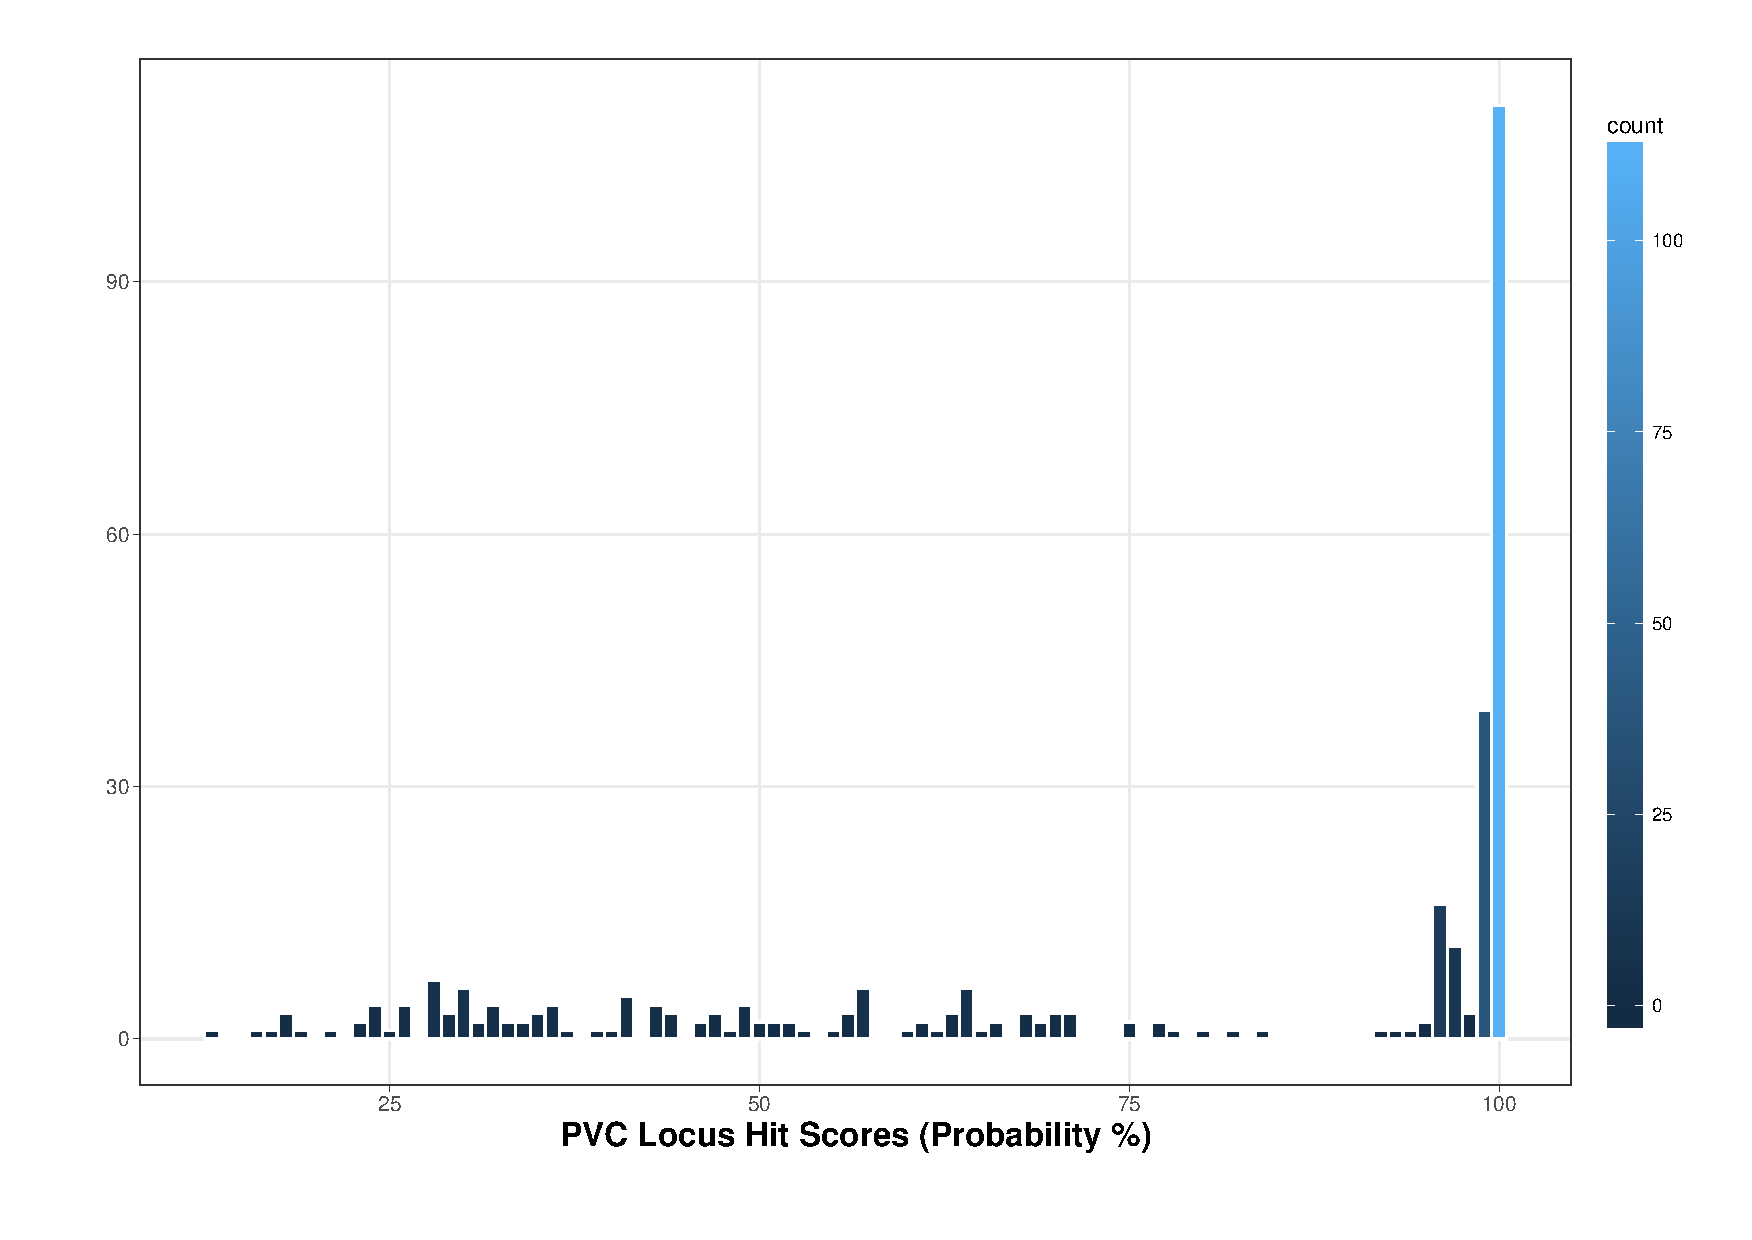
\includegraphics[width=0.9\textwidth]{/Users/joehealey/Documents/Warwick/PhD/Thesis/chapters/chapter3/img/Probabilities.pdf}
	\captionsetup{singlelinecheck=off, justification=justified, font=footnotesize, aboveskip=10pt}
	\caption[HHPred orthologue match scores]{\textsc{\normalsize Distribution of match probabilities for PVC proteins.}\vspace{0.1cm} \newline A histogram of the ``Probability" score for approximately 350 PVC protein sequences. Bars are coloured according to the bin density. Around half of all the proteins are well profiled in this manner, with Probability scores over 80\%. The remaining proteins are distributed widely with a number of examples of proteins which remain with low scores and little to no informative matches.}
	\label{probhist}
\end{figure}


\subsubsection{Homology modelling, threading and structural refinement}
Protein structure modelling was performed using a local installation of the I-Tasser pipeline, on 12 virtual machines \citep{Yang2014, Roy2010, Zhang2008}. I-Tasser was chosen as it generates full length models (whereas some tools only produce models for regions adequately represented by sequence homology), and because it takes a somewhat hybrid approach to modelling, using threading templates, but also \emph{ab initio} molecular dynamics steps for modelling regions (or whole sequences) with no reliable sequence templates, and for final model refinement. I-Tasser is consistently ranked as one of, if not the best, modelling servers/algorithms in the international Critical Assessment of Structure Prediction competitions \citep{Moult2015}.

In most cases, I-Tasser returns 5 models (though sometimes only 1 if the models converge well). Where multiple models were produced, in all upcoming analyses and images the model with the lowest RMSD to the PDB entry identified as closest via HHPred is used. \vref{rmsdhist} shows the distribution of RMSD values obtained from the simulations matched to these structures. The majority of the simulations were able to score well against deposited structures, with RMSDs less than $\approx$10 \AA.

\begin{figure}[h]
\centering
\thisfloatpagestyle{IHA-fancy-style}
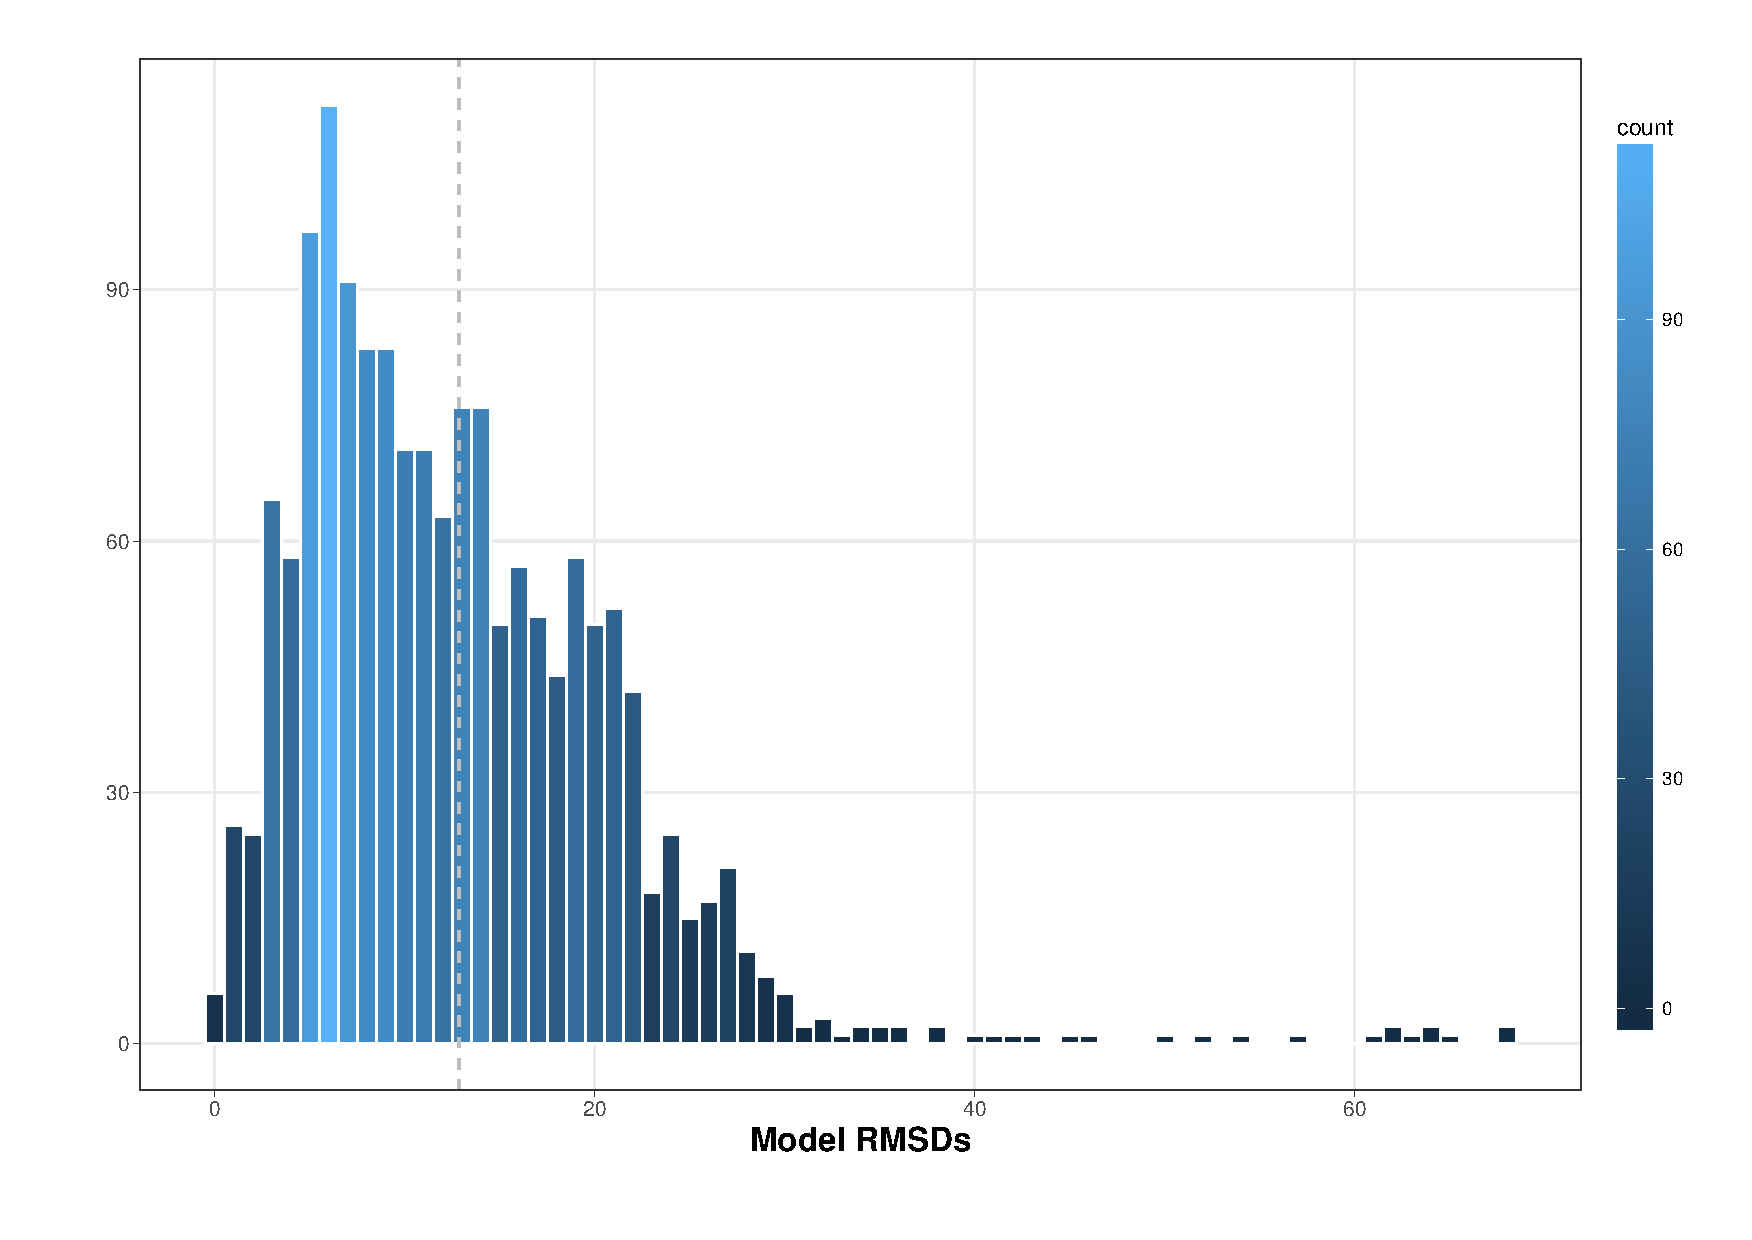
\includegraphics[width=0.9\textwidth]{/Users/joehealey/Documents/Warwick/PhD/Thesis/chapters/chapter3/img/RMSDhist.pdf}
	\captionsetup{singlelinecheck=off, justification=justified, font=footnotesize, aboveskip=10pt}
	\caption[I-Tasser model accuracy distribution - RMSD]{\textsc{\normalsize Distribution of atomic deviations for all simulated models.}\vspace{0.1cm} \newline A histogram of the Root Mean Square Deviation (in \AA{}ngstroms), between a modelled sequence and its closest structural match, as determined by HHSuite. RMSDs were calculated using the MatchMaker function within UCSF Chimera. Reasonable/useful RMSDs of less than $\approx$10 \AA{} are obtained for a significant proportion of the loci simulated. Bars are coloured according to the bin density.}
	\label{rmsdhist}
\end{figure}

That said, despite being the most widely used metric, RMSD is not a perfect measure of structure similarity, as it is prone to large RMSD values (indicative of poor fits) if just a few localised regions are not well matched, even if the protein overall shares similar topology. To this end, I-Tasser also produces calculations of "C-score" (confidence score) and ``TM-score" (template modelling score) \citep{Zhang2005}. I-Tasser provides additional data to assess the best models produced during its molecular dynamics steps, such as the cluster density, which represents the number of times a model passes through a region of 3D modelled space during its molecular dynamics trajectories. Thus the 3D space which is sampled most often is likely to represent the conformation of the most favourable models.

\begin{figure}[p]
\centering
\thisfloatpagestyle{IHA-fancy-style}
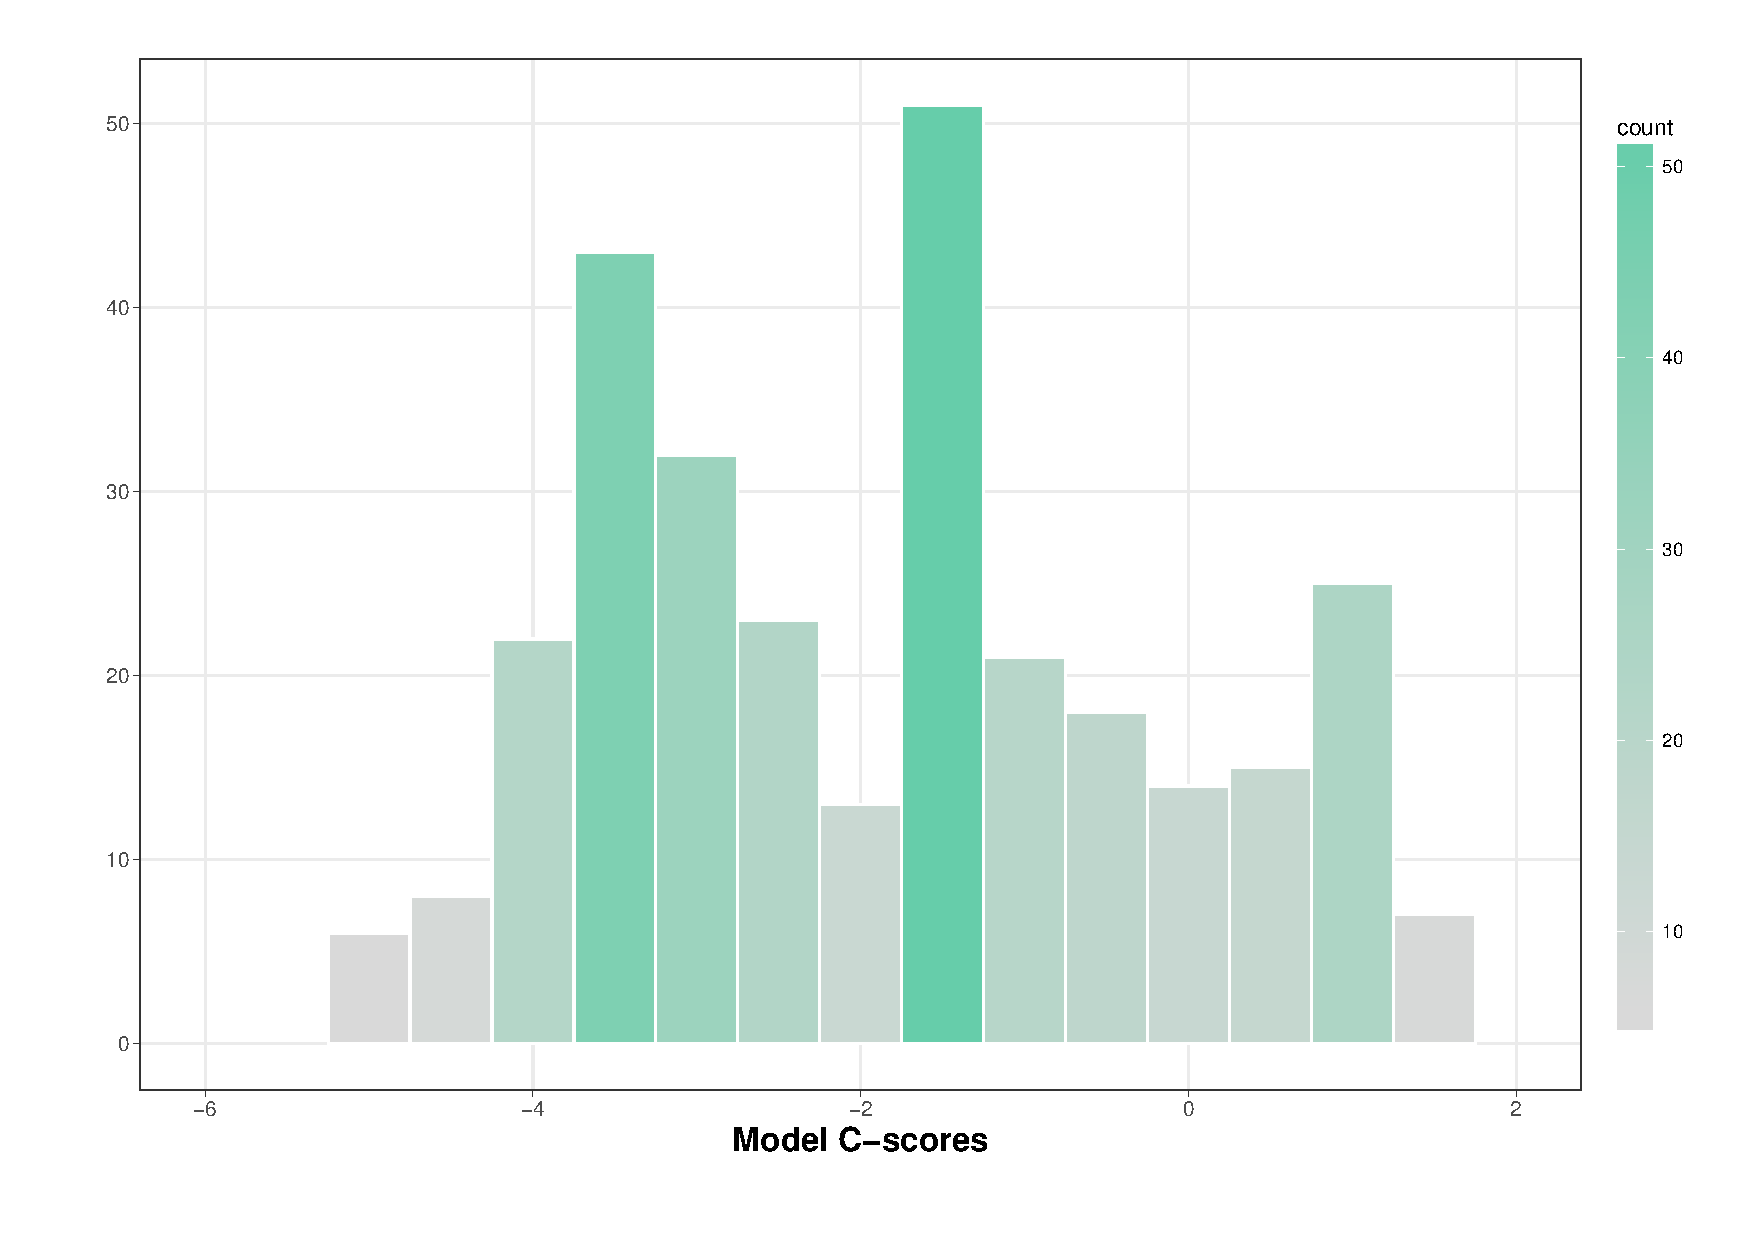
\includegraphics[width=0.9\textwidth, trim={0 30 0 10}, clip]{/Users/joehealey/Documents/Warwick/PhD/Thesis/chapters/chapter3/img/cscores.pdf}
	\captionsetup{singlelinecheck=off, justification=justified, font=footnotesize, aboveskip=7pt}
	\caption[I-Tasser model accuracy distribution - C-score]{\textsc{\normalsize Distribution of the ``C-scores" for all simulated models.}\vspace{0.1cm} \newline A histogram of the ``C-score" from I-Tasser. The C-score is a confidence score calculated internally by I-Tasser based on its confidence in the threading template alignments and convergence of the models. To a rough first estimation, C-scores of greater than approximately -2 indicate reasonable confidence. Approximately half of the models produced therefore have acceptable scores.}
	\label{cscorehist}
\end{figure}
\begin{figure}[p]
\centering
\thisfloatpagestyle{IHA-fancy-style}
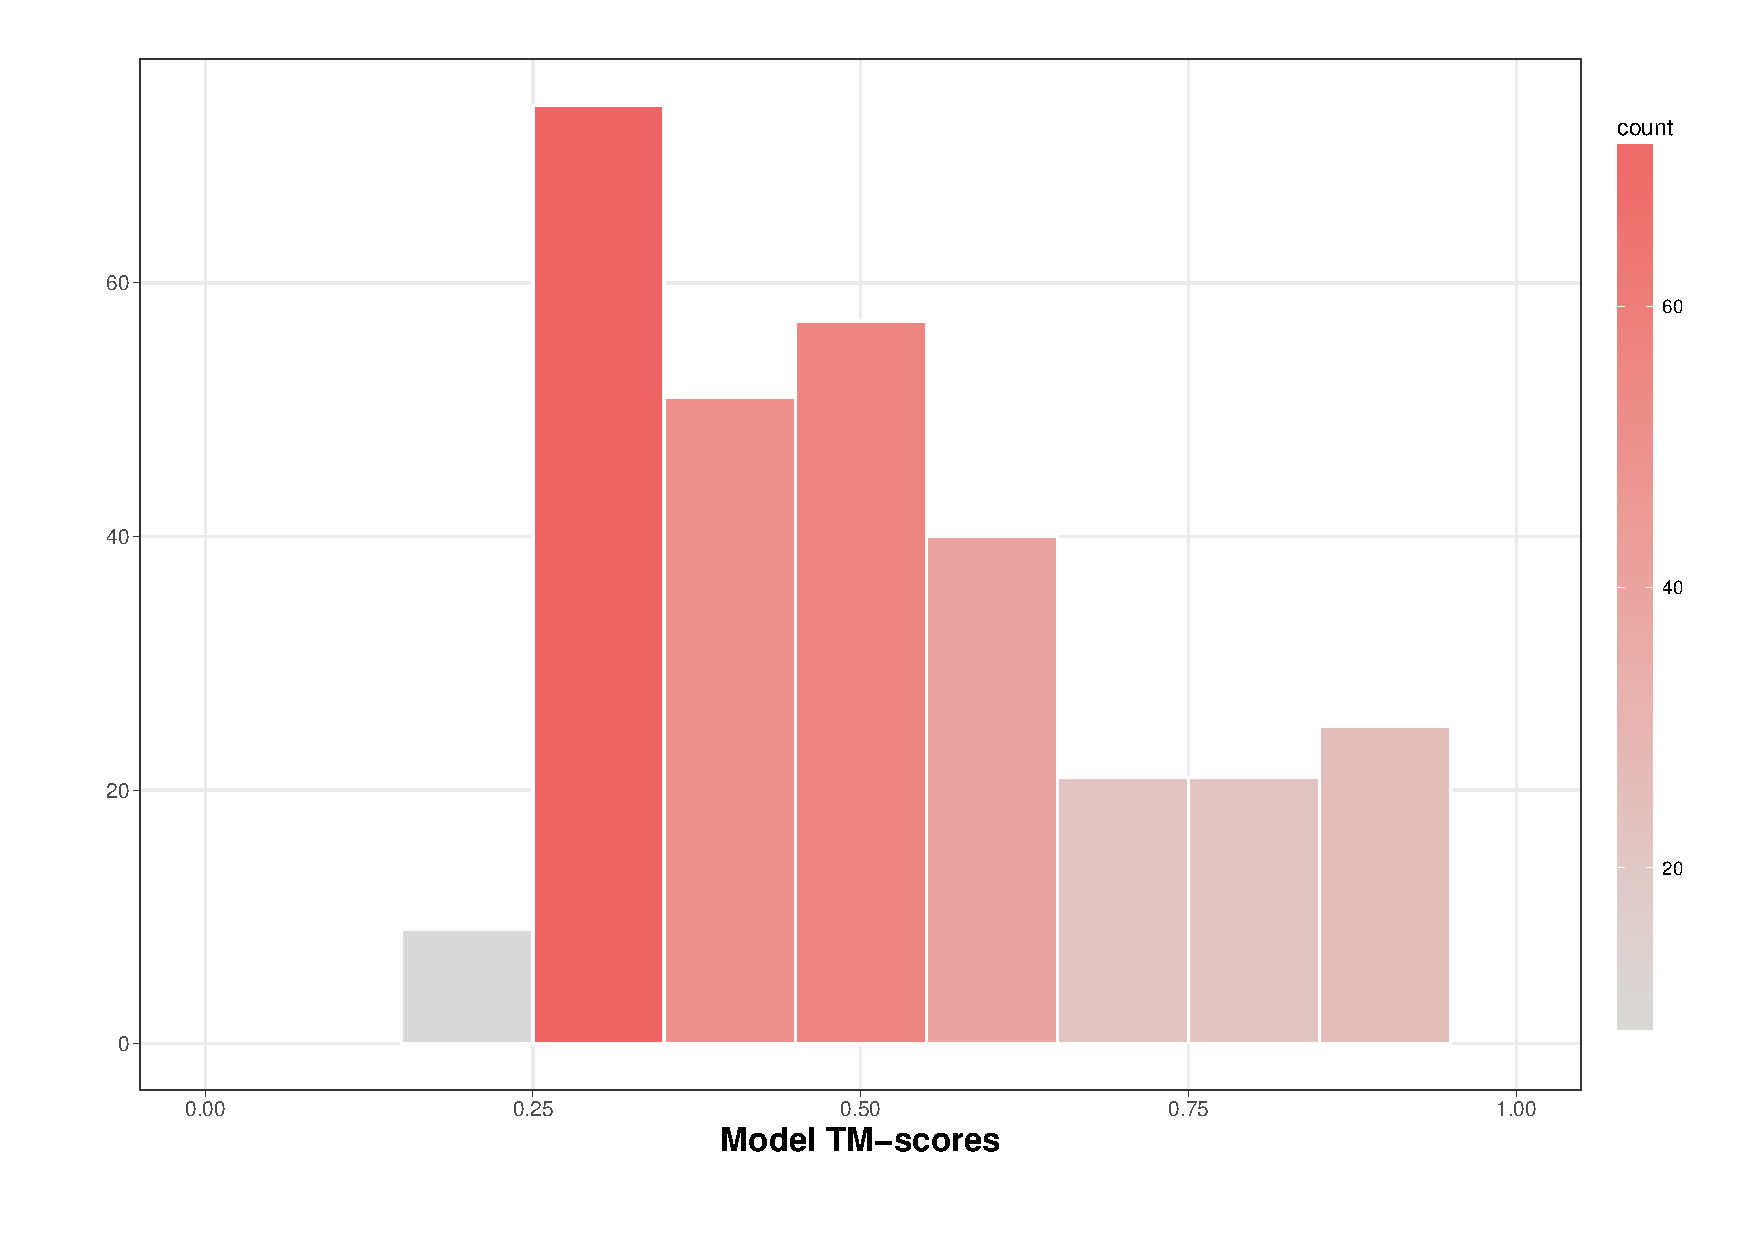
\includegraphics[width=0.9\textwidth, trim={0 30 0 10}, clip]{/Users/joehealey/Documents/Warwick/PhD/Thesis/chapters/chapter3/img/TMscores.pdf}
	\captionsetup{singlelinecheck=off, justification=justified, font=footnotesize, aboveskip=7pt}
	\caption[I-Tasser model accuracy distribution TM-score]{\textsc{\normalsize Distribution of Template Modelling score for all simulated models.}\vspace{0.1cm} \newline A histogram of the TM-score, between a modelled sequence and its closest structural match. TM-scores reflect how well 2 structures match globally, with less susceptibility to local deviations affecting overall score. The vast majority of protein models have TM-scores of greater than 0.25, an acceptable if slightly generous lower bound.}
	\label{tmscorehist}
\end{figure}

There are a large number of models with TM-scores of just over 0.2, (TM-score is in the interval $[0,1]$), which is considered the lower bound on a plausible match between structures \citep{Zhang2005}, suggesting that these protein structures may be of somewhat dubious quality. Roughly half of all modelled proteins have TM scores greater than 0.5 however, and these structures are therefore likely extremely well modelled. This correlates well, as expected, with the C-scores, where higher scores are indicative of better models. C-score is particularly useful when distance based metrics like TM-score and RMSD cannot be used, namely in situations where a template protein could not be identified at all.

It is important to mention however, that despite all these metrics, whether or not a model is useful depends heavily on the question at hand, since models which diverge from the reference structures may still have important/useful information in. Moreover, not all of the metrics correspond perfectly with one another (for instance, some models which have poorer C-scores, actually have good RMSD values). As the epigraph at the start of this chapter suggests, there is often no substitute for visually inspecting the models.

Eleven of the sequences attempted failed to simulate. Firstly, 8 sequences from the \Pasy{} Kingscliff genome failed to simulate due to the presence of ambiguous amino acids as a result of an older, lower quality, genome assembly. Three proteins were rejected for exceeding the upper amino acid length limit - I-Tasser's algorithms have a hard cut-off of 1500 amino acids. 

For the purposes of this chapter, structures are going to be assumed to be predominantly correct (positions of certain loops and small discrepancies notwithstanding). In cases where the simulations are likely spurious they will be noted in the discussion. That is to say, where good templates have been identified and plausible structures have been obtained, the electrostatics, general fold, and any inferences based on these will be assumed to be correct in the absence of truly resolved structures which could reveal unexpected differences. This is so that the chapter can focus on what might be learned from the models, rather than a lengthy discussion of whether the simulation quality is optimal.

\clearpage
\subsection{Exploration of the structure of PVCs by functional unit}

\subsubsection{The PVC tube}
\begin{figure}[h!]
\thisfloatpagestyle{IHA-fancy-style}
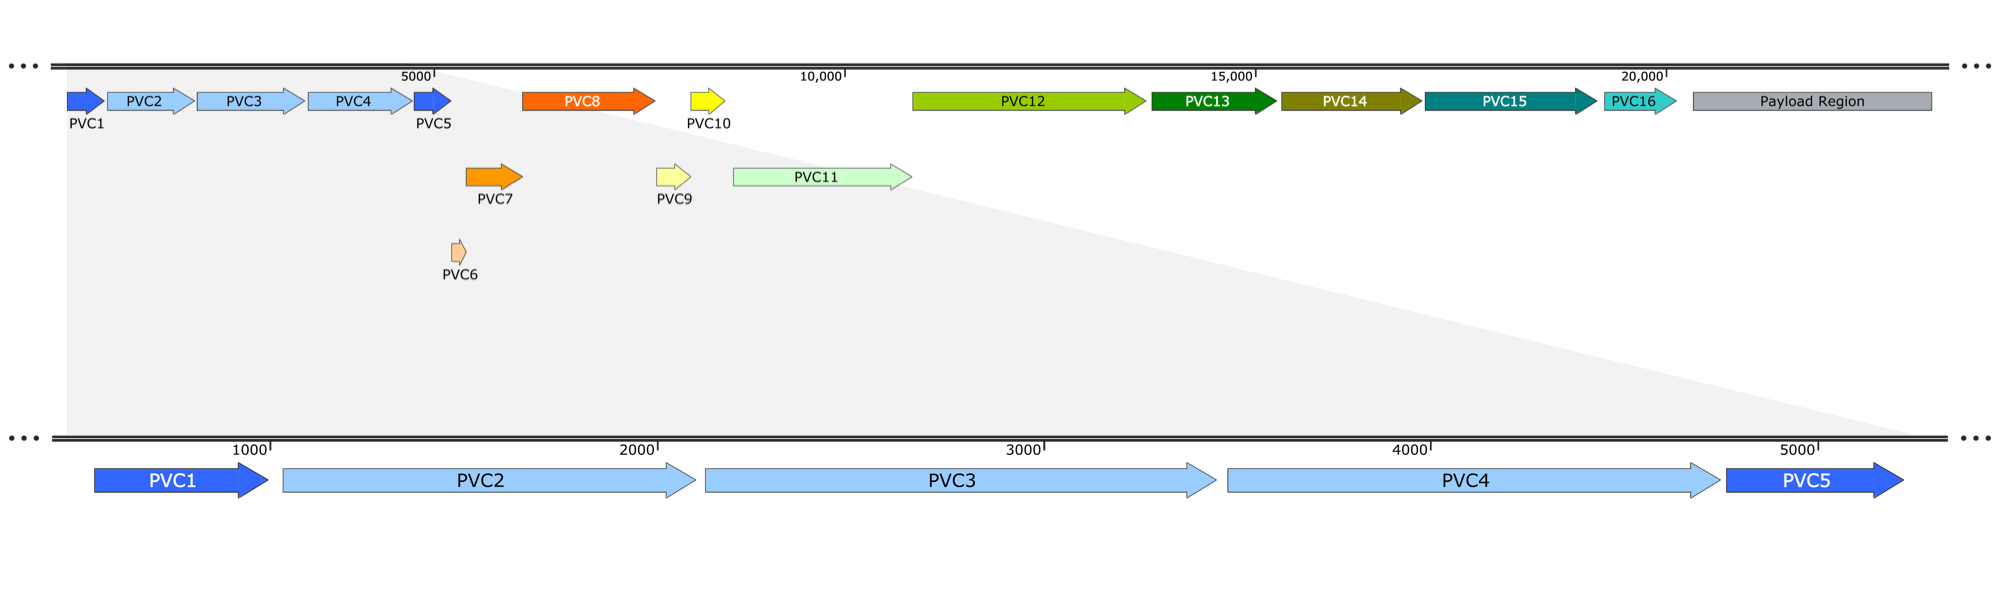
\includegraphics[width=\linewidth]{/Users/joehealey/Documents/Warwick/PhD/Thesis/chapters/chapter3/img/PVC1-5_expanded_map.png}
	\captionsetup{singlelinecheck=off, justification=justified, font=footnotesize, aboveskip=10pt}
	\caption[Tube protein region of a PVC operon]{\textsc{\normalsize The 5 loci that comprise the tube structure of a PVC.}\vspace{0.1cm} \newline \textbf{(Top)} The Pnf operon is used as an exemplar of the numbering of loci within an archetypal PVC operon, and 3 colourings are used to demarcate the `functional units' of an operon: blue - tube proteins, orange/yellow - spike complex proteins, green/cyan - the operon `core'. \textbf{(Bottom)} The 5 loci that give rise to the functional unit of the spike complex itself are blown up below as an aid to understanding the operon organisation and the proteins under discussion.}
	\label{PVC1-5map}
\end{figure}


Among the better annotated genes at the outset of this work, the first 5 loci of the PVCs, are predicted to match phage tail tube proteins of various sorts, though the existing annotations were not much more informative than this (for the rest of the operon the vast majority of which were ``hypothetical proteins"). With further inspection, these genes have become consistently annotated as T4-like virus tail tube or baseplate proteins (orthologs of gp6/gp19) and sheath proteins from the recently resolved \emph{Pseudomonas aeruginosa} R-type pyocin (see \vref{tubehomologs}). In some previous rounds of annotation, homologies to the Type 6 Secretion Systems of \emph{Edwardsiella tarda}, \emph{Vibrio cholerae}, and \emph{Burkholderia pseudomallei} were also detected for the inner sheath proteins (PVC1 \& 5), which underscores the original notion that PVCs seem to resemble a sort of hybrid, somewhere between a T6SS and a phage in sequence similarity.

From the resolved structure databases and literature, gp19 is known to be the inner sheath of the T4 bacteriophage (as can be seen in PDB IDs 5IV5 and 5W5F \citep{Taylor2016, Zheng2017}), and the outer sheath of PDB ID 3J9Q which corresponds to the resolved pyocin tube structure \citep{Ge2015a}. Over several iterations of homology searches with the HHpred suite, these 3 recent PDB depositions have come to be the most highly similar structures predicted.

\vref{tubehomologs} shows a summarised selection of the orthologues which HHPred has picked up over time. A full list of the most recent orthologies detected can be found in Appendix \vref{structural_appendix}.

\scriptsize
\rowcolors{2}{gray!10}{white}
\begin{tabularx}{\textwidth}{
>{\centering\arraybackslash} m{0.11\textwidth}
>{\centering\arraybackslash} m{0.11\textwidth}
>{\raggedright\arraybackslash} X
>{\raggedright\arraybackslash} X
}
\hiderowcolors
\captionsetup{singlelinecheck=off, justification=justified, font=footnotesize, belowskip=5pt}
\caption[HHPred hit summary for PVC1-5]{\textsc{\normalsize HHPred orthology summary for the tail tube proteins.}\vspace{0.1cm} \newline A summary of homology matches via HHPred for the first 5 PVC loci. The hits have varying degrees of confidence but have Probabilities greater than 60\% and E-Values of less than \sn{1}{-5}. They represent a `collapsed' set of common hits from all the variants for each locus. Hit scores for the inner sheath proteins (PVC1 and 5) are consistently lower than for the outer sheath proteins (PVC2-4) - all scores for the most recent analysis can be found in Appendix \vref{structural_appendix}.}\\
\label{tubehomologs}\\
Locus & PDB ID Hit & Structure & Component \\
\hline\hline
\showrowcolors
\hline

\rowcolor{white!10}                              & 5IV5 & Bacteriophage T4 & Baseplate wedge protein (gp6) \\ 
\rowcolor{white!10}                              & 5W5F & Bacteriophage T4 & Tail tube protein (gp19) \\
\rowcolor{white!10}                              & 3EAA & T6SS             & Inner sheath protein (Hcp/TssD)\\
\rowcolor{white!10} \multirow{-4}{*}{PVC1 \& 5*} & 4TV4 & T6SS             & Inner sheath protein (Hcp/TssD)\\
\rowcolor{gray!10}  PVC2, 3, \& 4                & 3J9Q & R-type Pyocin    & Outer sheath protein \\

\end{tabularx}
\hrule
\vspace{0.1cm}
{\tiny \noindent * PVC5 attracts the same 3 homology matches as PVC1, plus 4TV4.}
\normalsize

\vref{PVC1comparisons} and \vref{PVC2comparisons} showcase the similarities and differences in structure between the first 5 PVC loci and their nearest structural homologs either as determined via HHPred or previously shown in the literature. In addition, they also show a simulated structure from this study for the Antifeeding Prophage equivalent locus. The Afp is the closest orthologue when only DNA or amino acid sequence is considered, but no resolved structure exists (and therefore cannot be picked up by HHPred when using HMMs of the PDB database). \vref{PVC2comparisons} replicates this for an example of the outer sheath proteins.

Rather than show all the PVC loci compared to their homologs, where the PVC loci are similar, one example is shown (as in \vref{PVC1comparisons}) and then all the PVC variants are compared with one another in the subsequent \vref{PVC1-5_conservation}.

The inner sheath proteins from all these structures form a conserved pair of anti-parallel $\beta$-sheets which are sandwiched together approximately perpendicular to one another (with the exception of the T4 baseplate protein which appears to be an erroneous homology/annotation). They all exhibit a lower right hand extension positioned almost exactly in the centre of the amino acid chain (cyan/aquamarine) which would overlap the monomer adjacent to it within the tube hexamer. In the case of the T4 gp19 tube protein (chain F from PDB ID 5IV5), this is quite extended, along with a much longer protruding C-terminus (dark blue).

The matched PDB ID 5IV5 is the entire baseplate complex of T4, including part of the tube (and encapsulates PDB ID 5W5F, so there is a slightly redundant match), from the T4 phage. It seems unusual that many of the proteins match (at the sequence and secondary structure level) to chains within the model which are \emph{not} the tube, instead forming part of the baseplate complex, primarily gp6. It is clear from looking at the structures visually that these proteins are definitively homologues of the inner sheath proteins. On further inspection of the specific sequence matches detected by HHPred, it appears that what may have transpired is an error in the annotation of gp6 being attributed to some of the gp19 chains within the enormous 5IV5 PDB complex.

Inset in each figure is a pairwise distance matrix for alignments of the tube orthologues. Interestingly, though perhaps unsurprisingly, the sequence identity between the PVC and Afp is significantly better (a lower distance) than it is between either of them and the T6SS, T4 or Pyocin, despite the structures being extremely good matches, further reinforcing the message of this chapter that the sequence alone is insufficient to fully capture the subtleties of the evolution of these structures. Excluding the erroneous gp6 orthology, the remaining structures can be superimposed to an RMSD of 1.2 \AA{} or less.

For the outer sheath proteins, of which there are 3 in most operons, there is no ambiguity in their sequence matches, all having orthology to the R-type pyocin outer sheath under the PDB ID 3J9Q. The structures of the PVC2 locus from the ``Pnf" operon, and equivalent outer sheath proteins from other structures are also shown as in \vref{PVC1comparisons}, though they are less compelling matches than the pyocin at the sequence/HMM level (with the exception of the Afp, which is not detected by HHPred as the structures are unresolved), again highlighting that the sequence is not the be-all and end-all.

The outer sheath proteins are characterised by 2 outstretched termini which interlace with the adjacent monomers to form the contractile mesh over the rigid inner tube. In the case of the T4 tube, it's C-terminus actually forms an additional domain known as the ``protease resistant fragment", which the other structures lack \citep{Aksyuk2009}. The Type 6 Secretion System is unique amongst T4-like caudate structures, having a second outer sheath protein (TssB and TssC - known as VipA and VipB in the case of \emph{V. cholerae}), making the equivalent outer tube a heterododecamer. All the structures contain a pair of helices extending vertically which neighbour a pair of anti-parallel strands/sheets, that form the attachment interface to the inner tube electrostatically \cite{Ge2015a}.

Curiously, the 20 \AA{} Afp EM map depicted in \vref{afpstructure} seems to show protrusions of the sheath monomers radially, though the sheath proteins very closely match that of the R-type pyocin, as do the PVCs, and the R-type pyocin map lacks any such protrusions. Similarly, preliminary cryoEM data for the PVCs suggests a lack of any protrusions too. This might be indicative of an unknown third protein augmenting the exterior of the sheath, somewhat like the T6SS dodecameric arrangement.

The outer sheaths of all the non-T4, released/secreted, caudate structures are therefore much simpler proteins, representing perhaps a minimal functional unit capable of exerting the contraction, which is then decorated with domains such as the protease resistant fragment of T4 to confer further features to the sheath.

The pairwise sequence distances between the outer sheaths tell a similar story to the inner sheaths, with the PVC and Afp being the closest by some margin, compared to the remaining structures. However, the sequence distance is greater between the PVCs/Afps outer sheaths than it was for the inner sheaths. This will be due in part to the fact that the proteins are longer, but it seems that the surfaces of caudate apparatuses are open to modification, possibly to cope with different environmental stresses, or at the very least have some sequence redundancy. All proteins can be superimposed to an accuracy of less than 1.2 \AA, despite significant sequence differences.

\begin{figure}[p]
 \thisfloatpagestyle{augment}
\begin{subfigure}[H]{\textwidth}
  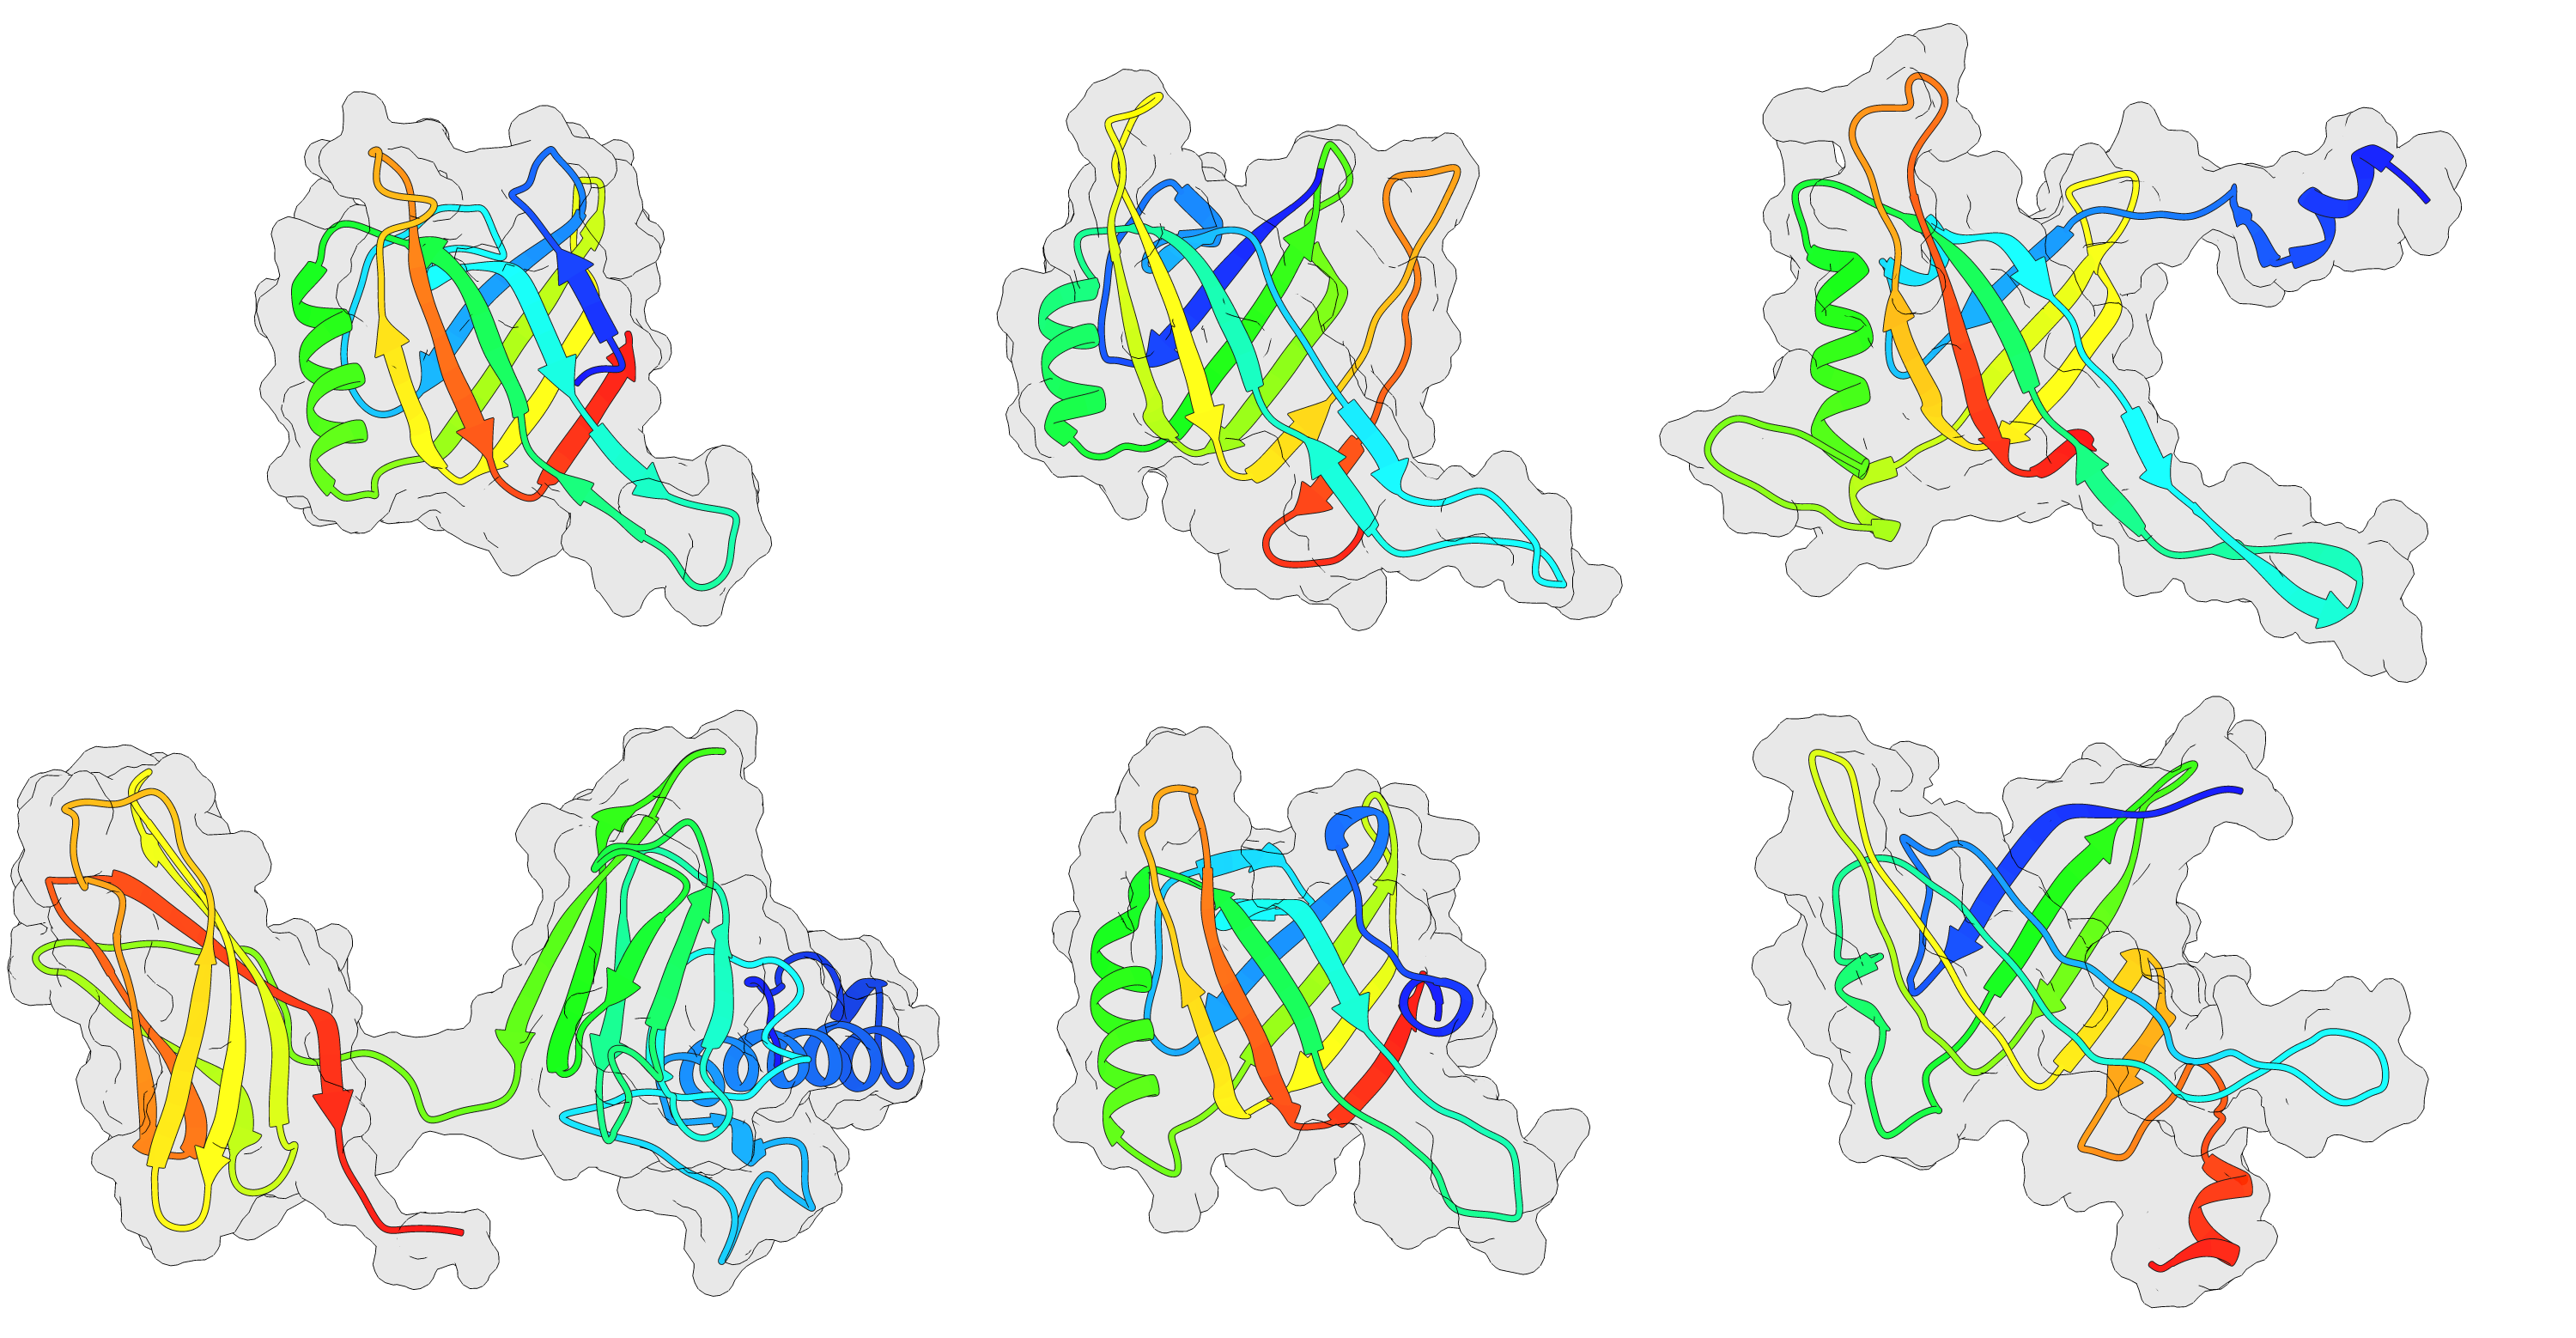
\includegraphics[width=\textwidth, trim={30 0 30 0}, clip]{/Users/joehealey/Documents/Warwick/PhD/Thesis/chapters/chapter3/img/PVC1_homolog_comparison.png}
 \put(-370,115){\small \centering PVC Simulation}
 \put(-227,115){\small \centering T6SS}
 \put(-105,115){\small \centering T4 Tube}
 \put(-370,-5){\small \centering T4 Baseplate}
 \put(-241,-5){\small \centering Afp Simulation}
 \put(-100,-5){\small \centering Pyocin}
\end{subfigure}
\begin{subfigure}[H]{\textwidth}
\tiny
\rowcolors{2}{gray!10}{white}
\begin{tabularx}{1.01\textwidth}{CCCCCCC}
\rowcolor{white!10}\multicolumn{7}{c}{Distance Matrix} \\
\hline
Model  & \multicolumn{6}{c}{Pairwise Distances}\\
\hline\hline
PVC                   & 0.000000 & 0.872483 & 0.885906 & 0.865772 & 0.255034 & 0.892617 \\
T6SS                  & 0.872483 & 0.000000 & 0.895706 & 0.876471 & 0.865772 & 0.892857 \\
T4 Tube               & 0.885906 & 0.895706 & 0.000000 & 0.846626 & 0.879195 & 0.877301 \\
T4 Baseplate          & 0.865772 & 0.876471 & 0.846626 & 0.000000 & 0.852349 & 0.880952 \\
Afp                   & 0.255034 & 0.865772 & 0.879195 & 0.852349 & 0.000000 & 0.899329 \\
Pyocin                & 0.892617 & 0.892857 & 0.877301 & 0.880952 & 0.899329 & 0.000000 \\
\end{tabularx}
\end{subfigure}  
 \captionsetup{singlelinecheck=off, justification=justified, font=footnotesize, aboveskip=20pt}
 \caption[PVC1 homolog comparisons]{\textsc{\normalsize Comparisons of the structure of PVC locus 1 to orthologous proteins.}\vspace{0.1cm} \newline An example model of PVC locus 1 from the PVCPnf operon of \Pasy{} ATCC43949. Here the structure is compared to (from top left to bottom right) the Hcp protein (5OJQ chain W) of the \emph{V. cholerae} T6SS, gp19 (5W5F chain V) from the T4 bacteriophage, gp6 also from T4 (5IV5 chain F), a simulated Afp1 structure from \emph{S. entomophila}, and an interior sheath monomer from the R-type pyocin (3J9Q chain V) from \emph{P. aeruginosa}. Models are shown `rainbow' coloured, from one terminus to the other, with a molecular surface `ghost'. It is evident that the 2 T4 proteins, despite being frequent sequence based matches to PVC1 (and 5), are not the closest matches in terms of structural conformation. The 3D model to accompany this page shows superimposed $\alpha$-carbon chain traces for all the structures (though without the T4 baseplate as its superposition is poor) - the PVC protein is rendered in thicker red wires/pipes, and the homologs in various monochrome shades. The inset table shows the all-vs-all pairwise alignment distances for the amino acid chains depicted }
	\label{PVC1comparisons}
\end{figure}

\begin{figure}[p]
 \thisfloatpagestyle{augment}
 \begin{subfigure}[H]{\textwidth}
 \includegraphics[width=\textwidth, trim={150 0 0 0}, clip]{/Users/joehealey/Documents/Warwick/PhD/Thesis/chapters/chapter3/img/PVC2_homolog_comparison.png}
 \put(-400,125){\small PVC Simulation}
 \put(-295,145){\small T6SS (A) \customarrow{2pt}{200}}
 \put(-250,125){\small T6SS (B) \customarrow{2pt}{200}}
 \put(-105,125){\small T4 Tube}
 \put(-400,-10){\small Afp Simulation}
 \put(-230,-10){\small Pyocin}
 \end{subfigure}
\begin{subfigure}[H]{\textwidth}
\tiny
\rowcolors{2}{gray!10}{white}
\begin{tabularx}{1.01\textwidth}{CCCCCCC}
\rowcolor{white!10}\multicolumn{7}{c}{Distance Matrix} \\
\hline
Model  & \multicolumn{6}{c}{Pairwise Distances}\\
\hline\hline
PVC       & 0.000000 & 0.890141 & 0.851613 & 0.856338 & 0.539548 & 0.845070 \\
T6SS VipA & 0.890141 & 0.000000 & 0.864516 & 0.883721 & 0.892655 & 0.898701 \\
T6SS VipB & 0.851613 & 0.864516 & 0.000000 & 0.845161 & 0.851613 & 0.864516 \\
T4        & 0.856338 & 0.883721 & 0.845161 & 0.000000 & 0.870056 & 0.875325 \\
Afp       & 0.539548 & 0.892655 & 0.851613 & 0.870056 & 0.000000 & 0.838983 \\
Pyocin    & 0.845070 & 0.898701 & 0.864516 & 0.875325 & 0.838983 & 0.000000 \\


\end{tabularx}
\end{subfigure}  
 \captionsetup{singlelinecheck=off, justification=justified, font=footnotesize, aboveskip=20pt}
 \caption[PVC2 homolog comparisons]{\textsc{\normalsize Comparisons of the structure of PVC locus 2 to orthologous proteins.}\vspace{0.1cm} \newline An example model of PVC locus 2 from the PVCPnf operon of \Pasy{} ATCC43949. Here the structure is compared to (from top left to bottom right) the VipA/VipB proteins (5OJQ chains c and m) of the \emph{V. cholerae} T6SS, gp18 (3J2N chain U) from the T4 bacteriophage, a simulated Afp2 structure from \emph{S. entomophila}, and an outer sheath monomer from the R-type pyocin (3J9Q chain A) from \emph{P. aeruginosa}. The T6SS structure uniquely comprises 2 distinct chains, along with some sequence extensions to the main chain. The T4 gp18 contains a considerable augmentation to its C-terminus consistent with protrusions that can be seen in \vref{t4structure}. Models are shown `rainbow' coloured, from one terminus to the other, with a molecular surface `ghost'. The 3D model to accompany this page shows superimposed $\alpha$-carbon chain traces for all the structures - the PVC protein is rendered in thicker red wires/pipes, and the homologues in various monochrome shades. The inset table shows the all-vs-all pairwise alignment distances for the amino acid chains depicted.}
	\label{PVC2comparisons}
\end{figure}


\myparagraph{Structural comparisons of duplicated and triplicated tube proteins}\label{duptrip}
An unanswered question is why \emph{Photorhabdus} has managed to maintain so many copies of what appear to be highly paralogous proteins in the tube region. Not only are the proteins paralogous within a single operon, but multiplied up by 5 or 6 times to account for the other operons, and somehow proteins with as many as 10 or more copies are somehow well preserved, when it might be expected that they would be open to drift.

\vref{PVC1-5_conservation} demonstrates the structural and sequence similarities between all 5 inner and outer sheath loci from the Pnf operon in \Pasy{} ATCC43949. There are some subtle structural differences (spans of loop structure etc.) between the loci, though they generally agree very well and this may be a result of the stochasticity in the molecular dynamics trajectories calculated by I-Tasser. PVC locus 1 does exhibit greater sequence variability compared to its `compatriot' PVC locus 5, though its overall fold is the same.

To explore this further, a comparison is made in \vref{PVC1-5_leastsimilar} between the least similar paralogues, as determined by their distances in the guide tree that accompanies the alignments, to show the most extreme differences (alignments can be found in Chapter \vref{bioinformatics_appendix}). In both cases (PVC1 and PVC5) the ``Lumt" operon from \Pasy{} Kingscliff and ATCC43949 respectively, present one of the pair of least similar sheath proteins. For the counterpart PVC1, the least similar paralogue is the inner sheath from the ``Cif" operon of \Pasy{} ATCC43949, and for PVC5 it is the tube protein of the ``Pnf" operon from the same genome.

\begin{landscape}
\begin{figure}[p]
 \thisfloatpagestyle{IHA-fancy-style}
 \centering
 \includegraphics[width=\linewidth, trim={0 0 0 0}, clip]{/Users/joehealey/Documents/Warwick/PhD/Thesis/chapters/chapter3/img/PVC1-5_composite.png}
 \captionsetup{singlelinecheck=off, justification=justified, font=footnotesize, aboveskip=10pt}
 \caption[PVC1 to PVC5 paralogue conservation comparison]{\textsc{\normalsize Comparisons of sequence conservation in inner and outer sheath paralogues.}\vspace{0.1cm} \newline Models of PVC1 to PVC5 for the Pnf operon are shown as front and rear rotations, coloured according to their per-column sequence conservation (as per the sequence alignments in Appendix \ref{bioinformatics_appendix}); rendered from high (green), to low (red), as per the inset scalebar. Structural differences are minimal, and sequence conservation is generally high, though PVC1 is slightly more variable (more blue sites) than its paralogue PVC5. Of the outer sheath proteins, the interior aspect is better conserved than the exterior, and all 3 loci exhibit increased sequence diversity.}
	\label{PVC1-5_conservation}
\end{figure}

\begin{figure}[p]
 \thisfloatpagestyle{IHA-fancy-style}
 \centering
  \includegraphics[width=\linewidth, trim={10 10 20 30}, clip]{/Users/joehealey/Documents/Warwick/PhD/Thesis/chapters/chapter3/img/PVC1-5_leastsimilar_composite.png}
 \captionsetup{singlelinecheck=off, justification=justified, font=footnotesize, aboveskip=10pt}
 \caption[Comparisons of the most dissimilar tube proteins]{\textsc{\normalsize Comparisons of the most dissimilar inner and outer sheath paralogues.}\vspace{0.1cm} \newline The most dissimilar homologues of the tube proteins (PVC1 to PVC5) and their structural/sequence differences. This panel highlights that, despite these being the least similar variants of the same locus, the structure is still well conserved, and thus the sequences are evidently at liberty to drift without compromising the PVC structure significantly. The variability in exterior sheath proteins, particularly PVC2 is highlighted.}
 \label{PVC1-5_leastsimilar}
\end{figure}
\end{landscape}



The interior facing side of the outer sheath is generally well conserved, as might be expected since it will need to interface with the generally well conserved inner tube proteins. The outer side of the sheath however, which represents the bulk of the structure which would be `exposed to the elements', shows a great deal of diversity in all 3 loci. Whether this is due to the even greater paralogy, and therefore increased possibility of drift, or to adaptation and `deliberate' diversification of the outer sheaths is not possible to say at this stage - though both present interesting hypotheses.\footnote{In \vref{PVC1-5_leastsimilar} The most distant PVC2 locus according to the guide tree is from the PVCPnf operon of \Pasy{} Kingscliff, but it failed to simulate due to ambiguous amino acids, so the next most dissimilar locus has been used instead - PVCUnit2 from \Plum{} TT01.}

A further observation can be made in \vref{PVC1-5_leastsimilar}. It has been known for some time that the PVC ``Lumt" operon in \Pasy{} ATCC43949 has deleted one of the structural loci (as have both examples of the PVC ``LopT" operon in \emph{P. asymbiotica} strains) - namely PVC3. However, in the Kingscliff ``Lumt" operon, the remaining PVC2 locus (which can be seen in the upper row of \vref{PVC1-5_leastsimilar}), appears to have lost the crucial twin helices that protrude upwards. The PVC4 locus for this operon is intact. \vref{lumt_outersheath} shows the remaining genes, and compares the sequence to the same operon in \Pasy{} ATCC43949. It appears that a similar deletion has occurred in both the ``Lumt" operons from \Pasy{} ATCC43949, and Kingscliff, however the Kingscliff PVC2 has undergone a gene split, resulting in 3 CDSs, despite the fact it has undergone the same deletion. This presents an interesting conclusion, as, if the genes are assumed to still be functional, it would mean that the outer sheath can be made up of 2 chains, similar to the Type 6 Secretion System. If the split genes \emph{are not} functional however, but the PVC itself is, this would prove that the remaining PVC4 is capable of `cis-complementing' the defunct genes, and therefore the existence of multiple gene copies may not simply be due to maintaining expression stoichiometry.


\begin{figure}[h]
 \thisfloatpagestyle{IHA-fancy-style}
 \centering
  \begin{subfigure}[h]{0.9\textwidth}
   \includegraphics[width=\textwidth, trim={0 0 0 0}, clip]{/Users/joehealey/Documents/Warwick/PhD/Thesis/chapters/chapter3/img/LUMT.png}
   \put(-227,102){\customarrow{0pt}{90}}
   \put(-170,20){\small Percentage Sequence Identity}
  \end{subfigure}
  \begin{subfigure}[h]{0.9\textwidth}
   \includegraphics[width=\linewidth, trim={70 30 70 60}, clip]{/Users/joehealey/Documents/Warwick/PhD/Thesis/chapters/chapter3/img/Lumt_outersheaths.png}
   \put(-380,0){\color{Goldenrod} \textbf{PAK\_02012}}
   \put(-280,0){\color{blue} \textbf{PAK\_02013}}
   \put(-120,0){\color{Emerald} \textbf{PAK\_02011}}
   \end{subfigure}
 \captionsetup{singlelinecheck=off, justification=justified, font=footnotesize, aboveskip=10pt}
 \caption[Deletions and domain splits in the ``Lumt" operon]{\textsc{\normalsize Outer sheath proteins of PVC ``Lumt" showing a domain split.}\vspace{0.1cm} \newline The outer sheath proteins of PVC ``Lumt" from the \Pasy{} Kingscliff operon are shown. The cyan model corresponds to PVC4, an intact outer sheath protein. The dark blue model is the same model as depicted in \vref{PVC1-5_leastsimilar} in the top row for PVC2. The 2 helices that protrude from the top in other proteins are missing, instead being present as a gene split, depicted as a separate chain in yellow. The arrow in the upper alignment panel shows the gene split in in the Kingscliff ``Lumt" operon, and is compared by sequence identity to the equivalent operon in the ATCC43949 strain (just the first 6 proteins of the operon). }
 \label{lumt_outersheath}
\end{figure}


\myparagraph{Electrostatic comparisons amongst tube proteins}
There do not appear to be obvious structural or fold differences that seem likely to lead to functional differences between these paralogues accounting for their maintenance. Perhaps then, the proteins may largely preserve their structure, but the differences brought about by diverse sequence manifest in electrostatic potentials which are in some way key to the structure of the PVCs. Given that the PVCs are proposed to carry different payload proteins with variable biophysical characteristics, there would stand to be 2 hypotheses: one, that the tube lacks any specialisation at all, allowing for many different payload to pass through, which appears to be the observed phenomenon for the T6SS \citep{Ge2015a}, or alternatively, each PVC is adapted in a particular way to its cognate payloads.

In \cite{Ge2015a}, comparisons are made regarding the electrostatics of the tube interiors, where they reason that the R-type pyocin, as a proton conducting apparatus, has a largely negative charge in order to convey such ions. Similarly, they remark that the inner sheath of the T6SS is mixed/neutral overall to cope with conveyance of diverse cargoes, and conversely that the interiors of the PS17 and $\lambda$ phages are mostly negative to convey DNA. This latter point seems as though it may be incorrect however, since the rendered, resolved, structure of the T4 tube, which conveys dsDNA, is extremely highly negatively charged - a rational for this might be a sort of `electromagnetic levitation' so that the DNA runs through the tube somewhat like a Maglev train, without `sticking' to the walls. \vref{inner_sheath_electrostatics} replicates a similar analysis for both inner tube proteins (PVC1/5), and the orthologues identified earlier (without the gp6 monomer and with PVC5 in its place however). Some potential structural differences are more apparent between PVC1 and 5 in this hexameric arrangement, but as its largely tied to loop structures, it is unadvisable to set too much store by it.


\begin{figure}[h]
 \thispagestyle{augment}
 \centering
   \includegraphics[width=\textwidth, trim={20 -20 20 -40}, clip]{/Users/joehealey/Documents/Warwick/PhD/Thesis/chapters/chapter3/img/Inner_tube_electrostatics.png}
   \put(-272,248){Coulombic potential}
   \put(-370,125){PVC1}
   \put(-233,125){T6SS}
   \put(-92,125){T4}
   \put(-370,0){PVC5}
   \put(-227,0){Afp}
   \put(-102,0){Pyocin}
 \captionsetup{singlelinecheck=off, justification=justified, font=footnotesize, aboveskip=10pt}
 \caption[Electrostatics of the inner sheath (cutaway)]{\textsc{\normalsize The Coulombic potentials of caudate structure inner sheaths.}\vspace{0.1cm} \newline The various inner sheath protein orthologues are rendered by their Coulombic electrostatic potential (i.e. charge), from strongly negative (dark red) through neutral (white with transparency) to strongly positive (dark blue). In consensus with the study of \cite{Ge2015a}, the R-type pyocin has a neutral to moderately negative charge in the interior. The sheath hexamers are shown as cut-aways (translucent grey faces show the `cut' path). The T6SS has mostly neutral charges (and a mixture of positives and negatives). The T4 tube appears to be overwhelmingly negatively charged, c.f. Ge et al.'s findings for the $\lambda$ and PS17 phages which were seemingly positively charged. The PVC (in both loci) and Afp, have similarly neutral-to-negative charges. In the case of PVC1, a halo of greater negative charge appears around the top, which is discussed further subsequently. The augmented reality model to accompany this figure shows the PVC1 hexamer in full 3D to give an idea of the all round electrostatics and structure.}
 \label{inner_sheath_electrostatics}
\end{figure}

Amongst all PVC1s there does not appear to be a great discrepancy in the surface potentials. All are largely negatively/neutrally charged. There are a few cases where some more prominent positive charges appear. In the case of PVC1, the exterior of the inner sheath is highly negatively charged. However, there is a prominent difference with PVC5, as it maintains a neutral and even positively charged exterior by comparison. This is surprising as it would be expected that if each monomer has to interact with an exterior sheath protein, and the sequences are largely conserved as shown previously, that both loci would carry similar charge profiles on this face.

\begin{figure}[h]
 \thispagestyle{IHA-fancy-style}
 \centering
   \includegraphics[width=\textwidth, trim={0 0 0 -30}, clip]{/Users/joehealey/Documents/Warwick/PhD/Thesis/chapters/chapter3/img/Pnf_top_bottom.png}
   \put(-271,318){Coulombic potential}
 \captionsetup{singlelinecheck=off, justification=justified, font=footnotesize, aboveskip=10pt}
 \caption[Electrostatic tube strata interfaces]{\textsc{\normalsize Polarities of the top and bottom faces of inner sheath monomers.}\vspace{0.1cm} \newline The electrostatic potentials of exemplar inner sheath monomers from PVC ``Pnf", loci 1 and 5. PVC1s exhibit predominantly positive charges on the `top' and `bottom' faces (the faces between disks of the tube), whilst PVC5s exhibit predominantly negative charges. This suggests that the 2 loci may form alternating hexameric stacks to assemble the tube in a directed manner like so: \texttt{(++)(--)(++)(--)}, where \texttt{(+-)} represents a monomer and its charges at either end.}
 \label{PVC1-5_charges}
\end{figure}



There seems to be further subtlety to the structural assembly of the PVCs incorporating these proteins, as the other predominant electrostatic pattern shows that PVC1 has predominantly negative charges at its `top' and `bottom', whilst PVC5 has predominantly neutral/positive charges, as demonstrated in \vref{PVC1-5_charges}. Therefore, one hypothesis is that the PVC is actually built from alternating stacks of PVC1-PVC5-PVC1-PVC5 with the negative and positive faces interacting. This is in contrast to, for example, the Pyocin tube, which has a prominent negative face, and a positive face within the same hexameric disk (visible in the bottom right of \vref{inner_sheath_electrostatics}, akin to bar magnets placed end-to-end, thus forms directionally controlled spontaneously self-assembling tube. As per the rest of the chapter so far \vref{PVC1-5_charges} shows the case for just one of the inner sheath pairs (PVC1 and 5 from PVC ``Pnf" again), but this largely holds for all 32 proteins. The side aspects of the proteins (not shown) demonstrate predominantly neutral charges, suggesting there is little significant within-disk ordering.

The outer sheath proteins remain something of a mystery. Not only is there often an additional copy of the gene, with very little obvious significant structural difference, but there does not appear to be drastic differences in charge between them. They all have predominantly neutral/positively charged interiors, but overwhelmingly negatively charged surfaces. Even with the sequence variability demonstrated in \vref{PVC1-5_conservation} and \ref{PVC1-5_leastsimilar}, there appears to have been a drive to maintain a negative overall surface charge. As an experimental indication of the models validity, an anion exchange chromatography protocol has been developed in the lab which relies on positively charged resins to retain negatively charged molecules and has worked well for purification of several PVCs to date.

As their inter- and intra-protomer interactions are more complex, \vref{PVC2-4_charges} shows a half-sheath where 3 of the 6 helical protomers have been scaffolded against the R-type pyocin's structure (a rise of 38.4 \AA, and a twist of 18.3\AA). Each protomer is made of one of the 3 paralogues from the ``Pnf" operon of ATCC43949. \cite{Ge2015a} suggest that the majority of interactions in the outer sheath are within a helical protomer, and this manifests in one of the outstretched `arms' of the outer monomers, carrying a negative charge which interacts with a positively charged groove at the neck of the monomer's two upstretched helices, below and to the left of it (as the helix is left handed).

\begin{figure}[p]
 \thisfloatpagestyle{augment}
 \centering
   \includegraphics[width=0.81\textwidth, trim={0 0 0 0}, clip]{/Users/joehealey/Documents/Warwick/PhD/Thesis/chapters/chapter3/img/Pnf_outer_tube.png}
 \captionsetup{singlelinecheck=off, justification=justified, font=footnotesize, aboveskip=10pt}
 \caption[Electrostatic tube strata interfaces]{\textsc{\normalsize Interior and exterior aspects of outer sheath protomer electrostatics.}\vspace{0.1cm} \newline The interior and exterior of the outer sheath proteins in biologically relevant positions/conformations are shown, scaffolded positionally against the R-type pyocin tube structure (PDB ID 3J9Q). All three paralogues share similar electrostatic profiles, with the tube interface as neutral/positive, but the exterior overwhelmingly negatively charged in all cases.}
 \label{PVC2-4_charges}
\end{figure}

The most compelling alternative hypothesis, certainly for the inner sheaths, is that one of the pair is specialised as an adaptor or collar. Given that PVC5 is translationally coupled to PVC6, another putative structural protein discussed in the next section, it might be likely that this is the case for PVC5. In \vref{PVC1-5_charges}, some greater structural differences do seem to manifest when viewed as a sliced hexamer. PVC5 has a slightly `squashed' confirmation, being somewhat wider than the PVC1 hexamer, and seems to have a slightly more restricted lumen suggesting that it is perhaps less suited to comprising the bulk of the tube. This fits with legacy 2D gel proteomic analysis which found PVC1 in abundance but lower levels of PVC5, and would also fit with the Coulombic patters noticed above in that PVC5 did not demonstrate the same outer aspect potentials as PVC1 (not shown explicitly), instead being much more neutral in charge. This might make sense if the hexamer doesn't have to interact with the outer sheath proteins like PVC1 might. \vref{PVCvsT4} shows a colour coded, stripped down, T4 baseplate complex, demonstrating that there are 2 additional proteins, gp48 and gp54 (red/orange), which form a transition between the inner tube and the spike, and resemble subtly modified inner sheath proteins. Interestingly, HHPred fails to attribute this orthology, instead matching primarily to the tube proteins themselves which may also have influence the homology modelling process. The figure shows the bulk of the baseplate hub in monochrome shades, the tube in yellow, and 2 fitted PVC proteins as white surface models. Outer sheath proteins are not shown.

Better RMSDs are obtained when matching PVC5 to gp54, than to gp48, so it is unclear whether there is another protein which fulfils the role of gp48 or whether PVCs have a simplified baseplate; certainly, their baseplates lack the vast majority of peripheral T4 baseplate proteins (which are omitted from the figure but the extent can be seen in the EM map). To complicate matters further, a recent paper by \cite{Renault2018} has demonstrated that, in the T6SS at least, the Hcp hexamers (equivalent to PVC1/gp19) interact directly with the face of gp27 in the spike complex explored in the next section. This may suggest that in this particular aspect, the PVCs are more similar to T4 than the T6SS, alternatively, PVC5 may form an adapted inner tube at the distal end of the tube, interfacing with terminator proteins to cap off the tube (similar to gp3-13-14-15 in T4 \citep{Fokine2013}, though no orthology to those proteins has ever been detected).

\begin{figure}[p]
 \thisfloatpagestyle{augment}
 \centering
   \includegraphics[width=\textwidth, trim={0 80 0 60}, clip]{/Users/joehealey/Documents/Warwick/PhD/Thesis/chapters/chapter3/img/PVC5_in_T4.png}
   \put(-130,460){\customarrow{-1pt}{0} gp19 / PVC1}
   \put(-135,410){\customarrow{-1pt}{0} gp54 / PVC5?}
   \put(-137,377){\customarrow{-5pt}{35} gp48 / PVC5?}
 \captionsetup{singlelinecheck=off, justification=justified, font=footnotesize, aboveskip=7pt}
 \caption[Comparisons of PVC5 to the collar components of the T4 phage]{\textsc{\normalsize Colour coded T4 baseplate collar proteins compared to PVC subunits.}\vspace{0.1cm} \newline The baseplate hub and collar of the inner tube for the T4 bacteriophage (PDB ID 5IV5 and EMDB 3374) are shown colour coded to identify the adaptor proteins that interface the spike complex (monochrome) with the tube (yellow). This chapter proposes that PVC5 is not actually a tube monomer, but instead may form one of these 2 strata of adapters in a simplified complex. The accompanying 3D model for this figure omits the surfaces and EM map as the geometry count is too high and transparency is not fully supported.}
 \label{PVCvsT4}
\end{figure}


\clearpage
\subsubsection{The spike complex}
\begin{figure}[h!]
\thisfloatpagestyle{IHA-fancy-style}
\includegraphics[width=\linewidth]{/Users/joehealey/Documents/Warwick/PhD/Thesis/chapters/chapter3/img/PVC6-11_expanded_map.png}
	\captionsetup{singlelinecheck=off, justification=justified, font=footnotesize, aboveskip=10pt}
	\caption[Spike complex protein region of a PVC operon]{\textsc{\normalsize The 6 loci predicted to comprise the spike and baseplate complex of a PVC.}\vspace{0.1cm} \newline The Pnf operon is used as an exemplar of the numbering of loci within an archetypal PVC operon, and 3 colourings are used to demarcate the `functional units' of an operon: blue - tube proteins, orange/yellow - spike complex proteins, green/cyan - the operon `core'. The 5 loci that give rise to the functional unit of the spike complex itself are blown up below as an aid to understanding the operon organisation and the proteins under discussion.}
	\label{PVC6-10map}
\end{figure}

The next 5 genes are a mixture of well resolved structures and complete enigmas. The most prominent gene in this cluster is PVC8, a VgrG/gp27-5 orthologue which is proposed to form the membrane puncturing spike at the tip of the tube. A complex of miscellaneous baseplate proteins and the spike itself are proposed to be a kind of `nucleation' site for the initial assembly of the tube. Given their syntenic position and the fact that several of the genes are translationally coupled, it seems likely that they may all have roles in the structural basis of the tube, likely within a collective collar/baseplate. PVC6 is actually translationally coupled to PVC5 in the `tube unit' of the operon, but without any good orthologies to suggest possible functions, the best hypothesis is that it may form an adapter or collar protein which interfaces the inner tube with the spike protein, since there is a transition at this interface from the 6-fold symmetry of the tube, to 3-fold in the spike complex.

A number of the (extremely weak) orthologies detected for PVC loci 6 and 7 seem to suggest enzymatic domains so it may be the case that these proteins are involved in the assembly of the PVC, but not in the structure itself.
\clearpage
\scriptsize
\rowcolors{2}{gray!10}{white}
\begin{tabularx}{\textwidth}{
>{\centering\arraybackslash} m{0.11\textwidth}
>{\centering\arraybackslash} m{0.11\textwidth}
>{\raggedright\arraybackslash} X
>{\raggedright\arraybackslash} X
}
\hiderowcolors
\captionsetup{singlelinecheck=off, justification=justified, font=footnotesize, belowskip=5pt}
\caption[HHPred hit summary for PVC6-10]{\textsc{\normalsize HHPred orthology summary for the putative baseplate and spike complex.}\vspace{0.1cm} \newline A summary of homology matches via HHPred for PVC loci 6-10. They represent a `collapsed' set of common or plausible hits from all the variants for each locus. Many of the loci in this section of the operon have poor orthologies detected. PVC8 and 9 are the only proteins with high scoring orthologies detected. All scores for the most recent analysis can be found in Appendix \vref{structural_appendix}.}\\
\label{tubehomologs}\\
Locus & PDB ID Hit & Structure & Component \\
\hline\hline
\showrowcolors
\hline

PVC6  &  Various & Various & Assorted enzymes/kinases (?)     \\
PVC7  &  5A3A    & n/a     & SIR2 Family metalloprotease (?)  \\
PVC8  &  2P5Z    & T6SS    & VgrG                             \\
PVC9  &  2IA7    & T4      & Tail lysozyme                    \\
PVC10 &  4JIV    & T6SS    & PAAR-spike tip (?)               \\
PVC11 &  3H2T    & T4      & Baseplate structural protein gp6 \\
\end{tabularx}
\hrule
\vspace{0.1cm}
{\tiny \noindent (?) denotes common or potentially plausible hits with very weak scores.}
\normalsize

\myparagraph{Enigmatic putative collar/baseplate proteins}
Proceeding in turn, PVC6 demonstrates no reliable orthologies whatsoever. Even with the more sensitive approach of using HMMs, the lowest E-value obtained for a hit is $>$1. The only potentially informative information available is that the proteins are all quite short, at only $\approx$61 amino acids, and the structural simulations resulted, almost universally, in a pseudo-L-shaped helix-turn-helix structure, with a degenerate position forming the start of the turn (all structures not shown for brevity). While this doesn't provide information much to go on, it may suggest that this protein forms an augmentation to another structural protein, or perhaps forms a kind of lynchpin to lock elements of the structure together, given its size and potentially simple shape.


In the case of PVC7, the hits are mixed, but dominated by matches (albeit weak ones) to an SIR2 family ADP-Ribsosyltransferase from \emph{Streptococcus pyogenes} \citep{Shore2000}, with the next most plausible hit being to an EssC-like chaperone of the \emph{Pseudomonas} Type 3 Secretion System \citep{Vogelaar2010}. While again, drawing too many conclusions from such weak similarities is unadvisable, it may be the case that these hits indicate that PVC7 has a role in assembly rather than the structure itself, potentially though some enzymatic or chaperone-like mechanism. Since the structural proteins are typically identifiable through structural homology, it is possible that PVC7 does not contribute directly to the structure proper. It is a much larger protein therefore the models simulated are likely among the more spurious, and they do indeed have some of the larger RMSDs to even the closest HMM matches (on the order of $\approx$20 \AA). Unfortunately, both PVC6 and 7 remain a mystery, and are therefore prime candidates for structural resolution and mutagenesis studies.

\myparagraph{The putative spike complex and PVC baseplate hub is more reminiscent of the T6SS}
This chapter proposes the idea that this section of the operon is made up of proteins which contribute to a baseplate and spike complex in some form or other. This may not be the case for the enigmatic PVC6 and 7, but almost certainly is for PVC8, 9, and potentially 10. Firstly, PVC8 has long been identifiable as a structural orthologue of the VgrG class of trimeric `spikes' which sit atop the inner tubes of every caudate structure identified to date. In T4, this spike is comprised of gp27 which forms a sort of trimeric adapter which interfaces with the hexameric tube, bridging the difference in symmetry. As mentioned in \vref{introduction}, VgrG's can be decorated with many additional functional domains (also forming toxins in their own right in some cases). The models obtained here indicate that PVCs employ a simplified spike complex, closer in structure to a T6SS like that of uropathogenic \emph{E. coli} \citep{Leiman2009}.

\begin{figure}[p]
 \thisfloatpagestyle{IHA-fancy-style}
 \centering
 \includegraphics[width=0.75\textwidth, trim={0 0 0 0}, clip]{/Users/joehealey/Documents/Warwick/PhD/Thesis/chapters/chapter3/img/spikes.png}
 \captionsetup{singlelinecheck=off, justification=justified, font=footnotesize, aboveskip=10pt}
 \put(-265,400){PVC}
 \put(-280,240){T6SS (UPEC)}
 \put(-265,10){Afp}
 \put(-110,350){T6SS (\emph{Pseudomonas})}
 \put(-75,10){T4}
\caption[PVC8 is the major spike complex of a PVC]{\textsc{\normalsize The PVC8 spike complex compared with homologues from T4, T6SS and Afp.}\vspace{0.1cm} \newline As one of the most distinctive proteins in the operon, annotations for this protein have proven reliable, however VrgG-like spikes are well known in the literature to be variable and share little sequence similarity. PVC spikes appear more like a simplified T6SS than like T4.}
	\label{spike}
\end{figure}


Particularly prominent appears to be the loss (in the non-T4 complexes) of the `wings' that the T4 spike exhibits, flanking the extended ``$\beta$-prism". \cite{Kanamaru2002a} identified these as tail spike lysozyme domains of the gp5 protein, which T4 is proposed to use to `chew through' the peptidoglycan cell wall of target bacterial cells. With no cell wall to negotiate in eukaryotic targets, it stands to reason that the T6SS, PVCs and Afps have lost this (though the T6SS does mediate some prokaryotic interactions as well, so may have other mechanisms it can substitute in to solve this problem). In T4, the structure is comprised of 2 separate proteins, gp27, which forms the `OB-fold' at the base of the structure and gp5 which contains the lyosozyme domain and forms the prominent $\beta$-prism at the very apex of the spike. In the simulations, this upper prism area is less well defined, and is even unresolved in the crystallised VgrG from the uropathogenic \emph{E. coli}. Based purely on protein chain length however, it does appear that the stretch of prism in the PVCs and Afps might be shorter. As a further example of the sequence variability and apparent potential for drift or adaptation of the VgrG-like spikes, the distance between the PVC and Afp orthologues is comparatively higher than for other loci studied so far, even with very similar tertiary structures among orthologues. 

\myparagraph{A new suggested role for PVC9 in tube initiation}
PVC9 has also been identified by sequence searches and annotation, as an orthologue of the PDB ID 2IA7, which has been listed as a putative tail lysozyme. This has always been a point of some confusion though, as it is not clear what role a lysozyme would have in the biology of PVCs, since they have never demonstrated any antimicrobial activity. With the loss of the gp5-like lysozyme domain in the PVC8/VgrG/gp27-5 orthology locus, it seemed that this might present a domain split, and that this domain had moved to a locus of its own. Nevertheless, with no cell wall to act upon in anti-eukaryotic virulence, the only other hypothesis proposed was that this may be a mechanism of release for the PVCs, by degrading the host bacterium cell wall. This also seemed some what unlikely, since the locus is carried squarely within many other putatively structural proteins.

On inspecting the structures, PVC9 candidates do indeed closely resemble the best HMM hit, PDB ID 2IA7, a putative tail lysozyme from \emph{Geobacter sulfurreducens}. However, they also closely structurally match the gp25 baseplate initiator protein of the T4 bacteriophage (PDB ID 5IW9), even though the E-value for this match (whilst still good) is 3 orders of magnitude greater (worse). \vref{initiator} demonstrates the similarity between an example PVC9, the \emph{G. sulfurreducens} structure, and gp25 of T4 in purple, blue and orange respectively. The RMSD between the putative lysozyme and the example PVC9 used is 1.2\AA, whilst between PVC9 and the gp25 PDB ID 5IW9 is less than 0.3\AA.

\begin{figure}[h]
\thispagestyle{IHA-fancy-style}
\centering
\includegraphics[width=0.8\textwidth, trim={50 10 60 0}, clip]{/Users/joehealey/Documents/Warwick/PhD/Thesis/chapters/chapter3/img/PVC9_gp25.png}
\captionsetup{singlelinecheck=off, justification=justified, font=footnotesize, aboveskip=10pt}
\caption[PVC9 as a tube initiator candidate]{\textsc{\normalsize PVC9 compared to a putative lysozyme and tube initiator.}\vspace{0.1cm} \newline PVC9 (purple), structurally compared to PDB ID 2IA7, a putative lysozyme (blue), and the T4 tube initiator protein gp25 (orange). Based on their structure similarity, PVC9 is likely a tube initiator protein, and this was not previously identified due to a spurious annotation of lysozyme on the better sequence match for PDB 2IA7.}
	\label{initiator}
\end{figure}


Since the role of a tube initiator protein is relevant to the structure and assembly of all caudate structures (as far as is known presently), and no other compelling candidates have been identified so far, PVC9 is therefore likely fulfilling this role. The descriptor ascribed to the PDB ID 2IA7 of a putative lysozyme is almost certainly incorrect.

\myparagraph{Identifying subtle hallmarks of spike tip ``PAAR" proteins in the baseplate cluster}
PVC10 has been another enigmatic protein for some time and still recruits matches to a number of different potential orthologues including proteins such as RNA polymerase subunits and Amyloid proteins. In just a couple of cases when querying the various PVC orthologues of this protein, homology was noted to ``PAAR"-repeat motif proteins. ``PAAR", or Proline-Alanine-Alanine-Repeat proteins are integral components of most caudate structures studied to date, but are extremely variable and difficult to detect. The T6SS alone employs a bewildering diversity of these proteins \citep{Shneider2013}. Curiously however, on first inspecting the sequences, there are few repeats to speak of when analysed by RADAR, and none of the orthologues even contain the ``PAAR" subsequence itself.

PAAR-repeat proteins sit at the apex of the extended $\beta$-prism of the spike complex, sharpening the otherwise slightly blunt face, down to a single atom's diameter potentially. \cite{Schneider2013} describe PAAR proteins in the case of model PDB ID 4JIV as being comprised of nine short $\beta$ strands, 3 of which form a base interacting with the rest of the spike complex following the $\beta$-prism conformation, and the remainder forming $\beta$ hairpins of different length.

The simulated models obtained are fairly poor facsimiles of \emph{bona fide} PAAR proteins of resolved structure, however, all of the models share some characteristics which support the hypothesis. The majority of models adopted a $\beta$-sheet dominated structure, which run head to tail, reminiscent of the $\beta$-prism conformation seen at the base of PAAR protein spikes, suggesting they augment the prism, if not form the spike itself. As these proteins are slightly longer than canonical PAAR proteins, it may be the case that they incorporate more of the $\beta$-prism in to the spike itself, which could account for the slightly shorter prisms seen in the PVC8 models, even taking in to consideration limitations in the simulation quality. This gives the models a similar triangular cross section to the PAAR proteins. Where the structures are not $\beta$-stranded they produce turn regions, which would provide the alternating strand-turn-strand conformation needed to enable $\beta$-hairpins like those seen in the resolved structures. These proteins possibly present a limitation for the simulation software, lacking good tertiary structure models and therefore resorting to largely molecular dynamics based approaches, which has given an energy minimised `collapsed' structure. However, \vref{PAAR} shows how the secondary structure and sequence of one of the putative PAAR protein model compared to the $\beta$-prism and PAAR protein from a \emph{Vibrio} T6SS. The conformations of the simulated structure are morphed on to the spike complex (in grey, PDB ID 4JIV). The largest span of amino acid similarity forms 2 of the major loops of the spike (shown in red on the upper monomer). There is some split structure which matches an additional $\beta$-strand region in dark blue (domains are split when an alignment gap is created). As mentioned, the PVC10 loci tend to be longer than canonical PAAR loci, and in this case, a significant proportion of the structure remains un-morphed on to the reference structure. Since one of the 3 major loops is missing, this suggests that part of the structure is too low similarity to be matched, but would mean that at least part of the unmatched structure (shown in white), could contribute to the spike. Nonetheless, the increased length of the protein, the dominant $\beta$-sheet, and roughly triangular cross section might suggest that the proteins contribute to the spike prism `stem' as well as the spike itself.

Despite the fact that long stretches which can align to the prism or the spike are identifiable (the red region of the spike and the cyan region of the prism map to the same 2 secondary structure spans in the models), the spike contains the longest matched stretch. Moreover, in order to form the prism 3 copies of the protein are needed. If the locus forms the spike as well as the prism, this would result in 3 spike domains which is unlikely. Moreover, to map the sequence on to the prism domain reference, many more sequence breaks were required.


\begin{figure}[h!]
\thisfloatpagestyle{IHA-fancy-style}
\centering
\includegraphics[width=0.8\textwidth, trim={30 20 10 300}, clip]{/Users/joehealey/Documents/Warwick/PhD/Thesis/chapters/chapter3/img/Coloured_spikes.png}
\captionsetup{singlelinecheck=off, justification=justified, font=footnotesize, aboveskip=10pt}
\caption[A putative conformation of spike tip proteins]{\textsc{\normalsize Exemplar PVC10 model with conformations mapped to the T6SS spike.}\vspace{0.1cm} \newline An example of a PVC10 locus obtained model is shown (twice) on the right hand side. These 2 models have had their conformations mapped on to the spike and $\beta$-prism domain from a T6SS on the left (PDB ID 4JIV). Unmapped stretches are shown in white and the reference structure is shown in grey. Colours indicate contiguously mapped stretches of sequence. Side chains are shown for metal coordinating amino acids which are relevant to \vref{PAARmetal}.}  
	\label{PAAR}
\end{figure}


Further evidence is present in the simulations for this loci's role as a spike tip; though they are certainly not fully correctly positioned, as the process of morphing conformations introduces strained geometries. The reference structure uses 2 histidine, and 1 cysteine residues to coordinate a metal atom at the tip of the spike, which holds the 6 strands of the 3 loops in place. In this model shown in \vref{PAARmetal}, one of the loops is not well modelled as mentioned, however in the 2 that were, one of the histidines is replaced by an arginine and the cysteine position can be superimposed over by a lysine (shown as ball-and-stick-models). This is consistent with the proposals of \cite{Shneider2013} who note that these residues may be replaced with ``similar or complementary metal-binding residues (arginines, lysines and glutamines) in more distant homologues suggesting that they also carry a metal ion roughly at the same position".

\begin{figure}[h!]
\thisfloatpagestyle{IHA-fancy-style}
\centering
\includegraphics[width=\textwidth, trim={0 0 0 0}, clip]{/Users/joehealey/Documents/Warwick/PhD/Thesis/chapters/chapter3/img/Coloured_spikes_metal.png}
\put(-96,177){\customarrow{2pt}{340} \color{red}  Arginine}
\put(-160,75){\customarrow{1pt}{330} \color{red}  Lysines}
\put(-118,89){\customarrow{1pt}{290}}
\put(-200,200){Histidine \customarrow{-6pt}{140}}
\put(-205,153){Cysteine \customarrow{-5pt}{150}}
\captionsetup{singlelinecheck=off, justification=justified, font=footnotesize, aboveskip=10pt}
\caption[Possible conservation of metal binding activity in spike proteins]{\textsc{\normalsize Evidence for potential conservation of metal binding in spike proteins.}\vspace{0.1cm} \newline The superimposed spike proteins preserve the localised positioning of metal coordinating residues (metal atom not shown). The reference T6SS structure is shown in white, the putative PVC spike protein in red. The positioning of an arginine in place of a histidine in the top most loop is very similar. The lower loop has some strained conformations so will not completely reflect the true structure, but conserves a lysine capable of metal coordination in place of a cysteine in the reference structure consistent with the hypothesis of \cite{Shneider2013}.}
	\label{PAARmetal}
\end{figure}

There is not much to be said for the last gene in this cluster, PVC11. It has had high quality orthology matches to the gp6 major baseplate hub protein of the T4 phage for some time. As a large gene, it likely contributes the bulk of the PVC baseplate which is certain to be drastically simpler than that of the T4. In T4, gp6 is critical to the conduction of the contraction signal, which likely accounts for why PVCs retain an orthologue. The only significant feature of these proteins appears to be that they have conserved N and C-termini, as seen in the alignments in Appendix \vref{bioinformatics_appendix}, but 3 of the 16 proteins studied (all belonging to the ``LopT" operon) retain an additional lengthy expanse of sequence. Interestingly, the ``LopT" operons are one of the few exceptions in terms of conservation of their `operon cores' which are explored in the next section. It appears that they do not harbour receptor binding `tail fibres', so perhaps the baseplate itself has some additional augmentation to replace them for allowing for binding/contraction, perhaps in a non-specific manner, as generalist toxin system.


\clearpage

\subsubsection{The operon core}
\begin{figure}[h!]
\thisfloatpagestyle{IHA-fancy-style}
\includegraphics[width=\linewidth]{/Users/joehealey/Documents/Warwick/PhD/Thesis/chapters/chapter3/img/PVC12-16_expanded_map.png}
	\captionsetup{singlelinecheck=off, justification=justified, font=footnotesize, aboveskip=10pt}
	\caption[`Core' protein region of a PVC operon]{\textsc{\normalsize The 5 loci comprising the `core' of a PVC operon with various functions.}\vspace{0.1cm} \newline The Pnf operon is used as an exemplar of the numbering of loci within an archetypal PVC operon, and 3 colourings are used to demarcate the `functional units' of an operon: blue - tube proteins, orange/yellow - spike complex proteins, green/cyan - the operon `core'. The 6 loci that give rise to the operon core are blown up below as an aid to understanding the operon organisation and the proteins under discussion. The `core' is a collection of conserved proteins present in almost all PVC operons, typically comprised of larger, single copy genes, some which are proposed to be structural, but also the proteins responsible for cell surface adhesion, and an ATPase which potentially loads payloads or recycles the tube apparatus.}
	\label{PVC11-16map}
\end{figure}

The final `module' of a PVC operon that this chapter will discuss is what is being termed here as the `operon core' (the chapter will ignore the payload region of the PVCs as that likely presents a thesis in itself). The operon core is typically reasonably well conserved, though poorly characterised - almost always containing 5 generally larger, single copy, proteins. 


\scriptsize
\rowcolors{2}{gray!10}{white}
\begin{tabularx}{\textwidth}{
>{\centering\arraybackslash} m{0.11\textwidth}
>{\centering\arraybackslash} m{0.11\textwidth}
>{\raggedright\arraybackslash} X
>{\raggedright\arraybackslash} X
}
\hiderowcolors
\captionsetup{singlelinecheck=off, justification=justified, font=footnotesize, belowskip=5pt}
\caption[HHPred hit summary for PVC6-10]{\textsc{\normalsize HHPred orthology summary for the putative baseplate and spike complex.}\vspace{0.1cm} \newline A summary of homology matches via HHPred for PVC loci 6-10. They represent a `collapsed' set of common or plausible hits from all the variants for each locus. Many of the loci in this section of the operon have poor orthologies detected. PVC8 and 9 are the only proteins with high scoring orthologies detected. All scores for the most recent analysis can be found in Appendix \vref{structural_appendix}.}\\
\label{tubehomologs}\\
Locus & PDB ID Hit & Structure & Component \\
\hline\hline
\showrowcolors
\hline

PVC12  &  Various      & Various & Assorted nucleotide binding (?)  \\
PVC13  &  1V1H / 2FKK  & T4      & Tail-fibre/baseplate             \\
PVC14  &  Various      & n/a     & Assorted                         \\
PVC15  &  5E7P         & n/a     & AAA+ ATPase                      \\
PVC16  &  Various      & n/a     & Assorted                         \\
\end{tabularx}
\hrule
\vspace{0.1cm}
{\tiny \noindent (?) denotes common or potentially plausible hits with very weak scores.}
\normalsize

\myparagraph{The enigmatic PVC12 remains one of the primary mysteries within a PVC operon}
PVC12, typically the largest protein in a PVC operon, has remained uncharacterised. Previous sequence annotations attributed weak similiarity to so called ``GGDEF domain" proteins. These proteins are ubiquitous bacterial regulators or signal sensors, and are proposed to bind or synthesise cyclic-di-GMP \citep{Ryjenkov2005}. Given its localisation in the operon it is tempting to assume it likely contributes another structural protein which is evidently quite unique, with no equivalent structures in the better characterised T4 or T6SS. With little to no informative orthologies detected nor any consistent structure between obtained models, PVC12 remains a mystery for the time being.


\myparagraph{The putative tail fibres equivalents of PVC operons}
PVC13 has long been of interest in the biology of PVCs, though the entirety of \vref{tailfibres} is dedicated to their experimental study, so they won't be covered in depth here. The tail fibres are the most diverse gene in the entire operon (also discussed in much more detail in the upcoming \ref{bioinformatics}), and are missing from the ``LopT" operons altogether. They appear to have split domain structures, and have attracted unusual anti-eukaryotic Adenovirus homologies fused to anti-prokaryotic phage domains over several bouts of annotation.

The simulations are of mixed reliability/quality, likely due in large part to their diversity resulting in the selection of various templates for the threading stages of the I-TASSER pipeline. \vref{fibre_models} shows a selection of the lowest RMSD models obtained. They have been symmetry modelled as trimeric proteins, since tail fibres are known to be trimeric only. While the finer details of the models is likely incorrect due to the sequence divergence, the gross architecture looks promising, and most interestingly of all, the hypervariable region of the alignment (annotated on \vref{tailfibremsa} in Chapter \ref{tailfibres}) can be seen prominently at one end of the structure (in red). At the opposite end, a largely conserved region can be seen which suggests that generally similar `mounting hardware' might be used to fasten the fibres to the tube baseplate.

\begin{landscape}
\begin{figure}[p]
 \thisfloatpagestyle{augment}
 \centering
   \includegraphics[width=\linewidth, trim={25 0 13 0}, clip]{/Users/joehealey/Documents/Warwick/PhD/Thesis/chapters/chapter3/img/PVC13s.png}
 \captionsetup{singlelinecheck=off, justification=justified, font=footnotesize, aboveskip=10pt}
 \caption[Conservation mapping off putative tail fibre structures]{\textsc{\normalsize Conservation mapping of tail fibres reveals a hypervariable binding region and conserved mounting region.}\vspace{0.1cm} \newline The conservation of amino acid positions for the extremely variable putative tail fibres of the PVCs. Tail fibres are responsible for target recognition and conveyance of the contraction signal to the contractile sheaths via the baseplate. PVC tail fibre models resemble the receptor binding tip (PDB ID 1PDI) of the short fibre of bacteriophage T4. The hypervariable domains are proposed to have homology to adenoviral motifs for eukaryotic targeting, and the high degree of diversity seen in the potential binding region speaks to the diversification of PVC variants against numerous target cell/tissue types. Inset is the T4 structure itself, a key to amino acid conservation and a small diagram for orientation since the perspective view of the tail fibres does not reproduce depth well in 2D. The accompanying model for this page shows a space-filling surface of the fibres rendered as above. }
 \label{fibre_models}
\end{figure}
\end{landscape}


\myparagraph{PVC14 as a putative `tape measure' protein}
The work of \cite{Rybakova2015} showed that Afp14, the equivalent locus to PVC14, is involved in determining the length of the tube structures. There is little known of the structural conformation of these proteins, compounded by the fact that they are proposed to span the length of a viral tail tube. This would mean that efforts to heterologously express and crystallise the proteins would not reveal their true state \emph{in vivo}. As discussed in the Introduction, these proteins are thought to exhibit a disproportionately high degree of helicity, as well as having distributed and broadly conserved hydrophobicities. This can be seen in resolved tape measure proteins such as that of PDB ID 5A20 \citep{Chaban2015}.

Inspecting the HHPred results for these proteins reveals no consistent hits, belying their variability, but many of them are to proteins such as a 3-helix bundle of \emph{S. aureus}, a heavily $\alpha$-helical nucleoporin of \emph{Saccharomyces} and typically helical membrane associated structures such as Photosystem II of \emph{Arabidopsis}. It is unusual that the homologies do not include hits to other tape measure proteins such as that of the phage SPP1 protein resolved by \cite{Chaban2015}, further reinforcing the idea that sequence homology is often an inadequate tool for these types of proteins.

Taking a selection of models obtained shown in \vref{tapemeasures}, it can be seen that there is little to no consistency in final globular structure (as would likely be the case with efforts to heterologously crystallise the proteins away from the tube), however, they are utterly dominated by alpha helical structures (the figures are coloured by secondary structure, with helix in magenta, $\beta$-sheets/strands in cyan, and coils in gray). Also rendered on the models is a hydrophobicity surface, which shows a homogenous distribution of hydrophobic/philic residues (orange/blue) across the structure, which is consistent with previously proposed orthologues.

Another indicative factor is that these proteins vary substantially in overall length, anywhere from $\approx$450 to $\approx$650 amino acids. As was also explored in the Introduction, \cite{Rybakova2015} and \cite{Pedulla2003} note that there is a strong linear correlation between final tube length and tape measure protein length. To a quick `back of the envelope' approximation using the trend identified, this would suggest that PVC tape measure proteins would be between $\approx$80 nm to $\approx$110 nm, based purely on sequence length - with the upper values roughly the same as the Afp itself. Estimates of the particle length from electron micrographs suggest they are closer to 150-200 nm though, so it may be the case that this trend is not entirely universal. The natural conformation for these proteins \emph{in vivo}, therefore, is likely extended helices, lying along the length of a growing tube, connected by short unstructured linker spans, somewhat like a length of rope with `$\alpha$-helical knots' along it.

\begin{figure}[h!]
 \thispagestyle{IHA-fancy-style}
 \centering
   \includegraphics[width=\textwidth, trim={120 0 120 9}, clip]{/Users/joehealey/Documents/Warwick/PhD/Thesis/chapters/chapter3/img/tapemeasures.png}
 \captionsetup{singlelinecheck=off, justification=justified, font=footnotesize, aboveskip=10pt}
 \caption[Conservation mapping off putative tail fibre structures]{\textsc{\normalsize Characteristic $\alpha$-helicity and hydropathy of `tape measure proteins'.}\vspace{0.1cm} \newline The simulated models for a selection of putative PVC14 tape measure proteins, revealing structure dominated, almost if not entirely, by $\alpha$-helix (magenta ribbons). Also rendered is a molecular surface coloured according to hydrophobicity/hydrophilicity, with the most hydrophobic residues in orange, and the most hydrophilic in blue. Tape measure proteins are proposed to have a largely conserved and homogeneously distributed pattern of residues with different hydropathy. The reference structure from T4 (PDB ID 1PDI) is simply rainbow coloured along the chain length. }
 \label{tapemeasures}
\end{figure}

\myparagraph{The conserved, characteristic, ATPase of PVC operons}
The ATPase carried by the PVCs and related structures are well conserved. In the original genome annotations, they are the only CDS which is given a `proper' gene name, rather than simply a locus tag. Namely, as an FtsH orthologue, the ATPases contain a characteristic protease domain at the C-terminus, and a comparatively variable N-terminus. The role the ATPase plays is still unknown, though in the T6SS it is responsible for recycling the tube structure. Since the proteins are conserved, but have unknown mechanistics within a PVC operon, they won't be covered in significant detail here.

Scrutinising the models obtained unsurprisingly reveals consistent structures between operons (not shown) (since the sequences are also highly similar). The active site of ATPase is preserved when compared to other known AAA+ ATPases, though the non-ATPase active site domain differs fairly substantially from structural and sequence orthologues such as PDB ID 5E7P for instance. The only remaining clue as to their role in PVC mechanistics, is that Hurst \emph{et al.} demonstrated that the ATPase is required for disease causing phenotypes in the Antifeeding prophage \citep{Hurst2004, Rybakova2013}, and that this is likely due to lack of assembly or misassembly of the complex.


\myparagraph{PVC16 as a tube terminator or cap protein}
Hurst and colleagues further demonstrated a role for the sixteenth gene of the operon in potentially capping the growing tube, leading to its growing length termination. Deletions and truncations of these proteins lead to aberrant forms of the structures. Similar to the putative tape measure proteins, no existing reliable structural or sequence orthologies are readily identifiable, with no E-values less than 1 that could be detected. The only consistent features of the obtained models are the presence of $\approx$3-5 helices, with the remainder of the structure being comprised of disordered turns. $\beta$-sheets were only observed in one or two models. If PVC16 is indeed a cap protein, it appears to be significantly structurally and sequentially different to any known functionally equivalent orthologues with resolved structures, and clues to its \emph{in vivo} conformation remain sparse.



\clearpage
\section{Discussion}
The intention of this chapter as a results chapter was to explore new hypotheses for roles of as-yet not fully understood loci within PVC operons, whilst also acting as an extended introduction, explaining the existing hypotheses and orthologies and orienting the reader for the specifics of the chapters to come. To be clear, this chapter does not claim to have \emph{solved} any structures; merely the intention was to exploit a rare opportunity to use high performance computing resources with impunity, in the hopes of providing data that might be used to inform practical experiments further down the line, such as targeted mutagenesis with the benefit of at least some structural understanding.

PVCs represent a hybrid between the T4 phage, R-type pyocins and T6SS like structures. More specifically however, they appear to resemble the different structures in different parts of the overall apparatus. For example, the outer sheath proteins of PVCs appear more like the T4 phage/Pyocin, than they do like the T6SS for instance, whilst the opposite is true for the spike complexes. Likewise, the PVCs carry the characteristic AAA+ ATPase which is also a typical hallmark of the T6SS, but is not the case for T4 phages.

Hopefully this chapter has also proven the statement made in the introduction, that sequence-based orthology studies are insufficient, particularly when dealing with protein folds which probably first originated in deep time (with the first phages). These fundamental fold structures which give rise to the inner and outer tubes for example, appear robust to reuse in all manner of translocation applications (DNA/protein/ions etc.). The co-opting bacteria exploit the redundancy and robustness of these structures to hone the surface properties such as hydropathy and charge to adapt to varied niches, all the while preserving an incredibly complex and elegant structure.

\vref{orthologysummary} summarises the new and existing proposed roles for the proteins within the PVC operons, though despite all the advancements made experimentally, and even hypotheses proposed here, there remain enigmatic proteins with few if any clues as to even a plausible role.


\small
\rowcolors{2}{gray!10}{white}
\begin{tabularx}{\textwidth}{
>{\raggedright\arraybackslash} m{0.3\textwidth}
>{\raggedright\arraybackslash} X
}
\hiderowcolors
\captionsetup{singlelinecheck=off, justification=justified, font=footnotesize, belowskip=5pt}
\caption[Summary of loci functions in PVC structural biology]{\textsc{\normalsize Summary of putative loci functions for PVC structural proteins.}\vspace{0.1cm} \newline A summary of the proposed primary roles for PVC structural loci. Loci with asterisks indicate new functions proposed as a result of this work, or new evidence which contributes to existing proposed roles.}\\
\label{orthologysummary}\\[-0.3ex]
Locus & Proposed structure/role in the PVC \\
\hline\hline
\showrowcolors
\hline
PVC1 & Inner tube   \\
PVC2 & Outer sheath   \\
PVC3 & Outer sheath (frequently deleted)   \\
PVC4 & Outer sheath   \\
PVC5* & Possible collar adapter  \\
PVC6 & Unknown (augment/lynchpin?)   \\
PVC7 & Unknown (Possible enzyme/chaperone?)   \\
PVC8 & Spike trimer   \\
PVC9* & Tube initiator   \\
PVC10* & PAAR-like spike augment   \\
PVC11 & Major baseplate protein   \\
PVC12 & Unknown   \\
PVC13 & Host binding tail-fibre chimeras   \\
PVC14 &* Tube `tape measure protein'   \\
PVC15 & Loading/Assembly ATPase   \\
PVC16 &* Tube terminator (?)   \\
\end{tabularx}
\normalsize

For the bulk of the PVC tube, it is interesting that the inner and outer tube orthologies do not share the same provenance. It might be expected that they should all match to the next closest structure (e.g. all matching to the \emph{P. aeruginosa} R-type pyocin), but instead the inner sheath proteins retain T4 hits. This potentially indicates that the inner and outer sheaths may be subject to different evolutionary pressures. Additionally, interior sheath proteins are smaller and better conserved. This may, therefore, demonstrate that \emph{Photorhabdus} is honing the exterior of the sheath in different environments. An appealing hypothesis, especially since legacy data has shown that different PVCs are deployed in very particular inducing conditions.

A difference in provenance for the inner sheath proteins compared to the outer sheath proteins is consistent with published observations that, for instance, the R-type pyocin is generally negatively charged to convey protons for depolarisation, and that the T6SS is comparatively neutral for conveyance of proteins \citep{Ge2015}. This is therefore indicative of the inner and outer sheath proteins potentially being under different selection pressures, reflecting their deployment environment (in the case of the outer sheath) and their cargo (in the case of the inner).

Why PVCs carry multiple copies of tube proteins has a curiosity for some time. The original speculative hypothesis for this was that, as the bulk of the structure, they would need multiple copies to provide stoichiometric ratios to the rest of the operon components (i.e. 2 proteins would be produced `per transcript'). There are flaws in this idea though. Firstly, the inner and outer sheaths are, to the best of our current knowledge, present in roughly equal parts, as hexameric concentric disks in an approximately 1:1 ratio. Yet, there are (normally) 3 outer sheath loci, and 2 inner sheath loci. Plus, the fact that at least one of these loci can be deleted with (as far as is known about their functional state) no consequence, suggests the stoichiometry is not that sensitive to disruption. From comparing the sequential and structural conservation, and biophysical properties of the tube proteins, the following alternative hypotheses for their maintenance are suggested. For the inner sheath proteins, there are prominent differences in the electrostatic nature of the subunits. This suggests that the tube is either made of alternating stacks of the different monomers, providing directionality to the tube, or increasingly likely, that PVC5 actually fulfils a more specific role. This role may be as an orthologue of gp48/gp54 in T4, as a collar/spike adapter, or possibly gp3 in the tail termination complex at the opposite, distal, tube end (though no crystal structures yet exist to compare to). There are slight contradictions here too however, as in the T6SS, a recent paper has shown that no such adapter/collar proteins are needed \citep{Renault2018}, and the inner tube can interface directly with the VgrG spike. Given that the tube appears more reminiscent of a phage than a T6SS, but the spike is conversely seemingly T6SS-like, only experimental structural resolution will yield the answer. Preliminary data and EM maps from the ongoing structural resolution collaboration with the Max Planck Institute in Dortmund (not shown) have suggested that the baseplate region might be more substantial than has been seen in either the Afp or R-type pyocin so far, which could indicate that it is more similar to a T4 phage. In which case, the likelihood of a collar adapter protein remaining is somewhat higher.

The outer sheath proteins remain somewhat of a riddle. Their less conserved outer aspects suggest that they are open to adaptation to their deployment niches. A `phage like' exterior, for instance, is likely to be significantly immunogenic in a higher eukaryote infection, which runs counter to \emph{Photorhabdus}' extensive efforts to suppress immune responses during infection (a theory proposed to explain the enormous repertoire of toxins that it carries). An appealing hypothesis therefore, is perhaps these nano-scale toxin delivery systems are adapted for use in these infections. The pronounced negative surface charges noted with all of the loci might also speak to a similar phenomenon, as previous publications have identified marked reduction in trypsin-based proteolysis of negatively charged particles compared with positive ones \citep{Liu1992}. Similarly, positively charged molecules have been shown to be preferentially endocytosed at greater rates \citep{Chung2007} - though admittedly neither of these studies focussed on proteinaceous entities. \cite{Hurst2004} demonstrated that Afp2 is required for formation of a toxic Afp. In several PVC operons a deletion in one of the 3 proteins which match to outer sheaths are observed. Initially, it was not obvious which of these 3 proteins, assumed to be equally paralogous, would be deleted in each case. It seemed unusual that 3 outer sheath CDSs would be required whilst only 2 inner sheath CDSs are ever present, if stoichiometry was the only explanation for their paralogy. On further inspection, it appears that the deletions in these outer sheath proteins is always PVC3 rather than 2 or 4. Unpublished communication from the Hurst lab has proposed that PVC4 may actually be a slightly modified variant of the outer tube. This may be such that it functions as an adapter protein at one end of the tube, possibly as a collar that interfaces with the baseplate.

Stepping through the operon, PVC6 and 7, the first putatively `non-tube' loci remain poorly characterised as no experimental work has been yet conducted which offers functional information, nor are there any published protein structures which offer up any insights based either on sequence identity or structural similarity. Consequently, these 2 loci are prime candidates for mutagenesis studies in future. PVC6 is a small locus, and it is possible that it is merely an artifact of gene prediction/annotation software. The fact that it is translationally coupled to both PVC5 and PVC7 suggests that its is probably unlikely, however, the significance of this coupling is still not yet understood. PVC7 matches very loosely to certain metalloprotease orthology, perhaps suggesting that it may have an enzymatic role rather than a structural role, but these hits are much too weak to speculate on to any real extent.

Moving on to PVC8, the exact conformation of the gp27-5/VgrG-like spike will potentially yield interesting data for further study. In the case of the T6SS, the spikes are known to frequently be augmented with other enzymatic activities and other toxins, functioning like a poison arrow rather than a syringe in some cases. The T6SS is both anti-eukaryotic and anti-prokaryotic, and the T4 spike is purely anti-prokaryotic. The PVC spikes are (as far as has been observed to date), purely anti-eukaryotic. This implies different evolutionary pressures on the protein, which may be manifested in subtle differences in the structures, since the membranes and internal cellular pHs of targets will vary. The pH within the target cell has been shown to be the cue for the spike complex to dissociate, `uncapping' the tube, and so the electrostatics of the structure and affinities between the monomers will potentially be subtly sensitive to the environments the complexes are deployed in, which may manifest in their sequences, substituting amino acids of particular electrostatic properties in accordance. As mentioned, the spike complex appears to be one of the areas of the operon where the PVCs are more similar to the T6SS than to the T4 phage, being somewhat simpler for lacking the lysozyme domain, but also being homotrimeric, unlike the T4 which is heterohexameric (gp27 and gp5).

A major remaining mystery within the operons is that of PVC12. Weak orthologies to nucleotide binding proteins does not provide much information to speculate upon. Even if the nucleotide binding potential is valid (which is far from certain), its role within the operon is still unknown. Given its syntenic position, the default assumption is that it too contributes to the structure. As typically the largest protein in the operon, a role in the overall structure would likely be fairly pronounced and one might expect it to be easier to identify. Similar proteins have not been seen in other caudate structures to date. Probably the best current hypothesis for its presence, and actually fairly considerable conservation, is as a regulator of the operon in some manner. The GGDEF domain which has been weakly identified within the protein previously is typically implicated in regulatory mechanisms in prokaryotes, but for the PVCs this too remains hugely speculative and weakly supported. PVC12 is another chief candidate for mutagenesis studies.



To briefly make note of the limitations of this approach, obviously the simulations presented in this chapter are of assorted qualities, and care must be taken when concluding anything from theoretical data alone. There is however, a sufficient body of related proteins for many PVC loci, such that comparative modelling can provide, and has provided, hypotheses and potential answers for a number of questions which are not answerable without resolving the structures either experimentally or otherwise. Homology modelling is a standard tool that is often reached for in many publications when the alternative is to have to laboriously resolve the structure (if it is even possible), but as George Box's famous aphorism goes: ``all models are wrong, but some are useful."

Some of the primary limitations of this approach are discussed below. I-TASSER is still a semi-template-based method, though it breaks down structures in to essentially meaningful chunks, rather than relying on a single overall structure too much. This is conceptually similar to finding `structural k-mers' - amino acid `words' which `spell out' a particular helix structure or span of $\beta$-sheet etc. Such methods may not be ideal for 2 opposing reasons which relate to the `morals' of this chapter. Firstly, sequence matches which are \emph{too good} will result in over-fitting of sorts. This will then provide a model of high confidence, which mirrors an existing structure, but that does not guarantee than \emph{in vivo} in the host organism, that that protein actually folds in the same way. As the example in the introduction (the protein G from \emph{Streptococcus}) makes plain, 2 proteins with extremely similar sequences can have entirely different folds. This is even before additional biological considerations are factored in, such as chaperones, whereby proteins of very similar sequence, but some with chaperons and some without, will likely lead to substantially different structures. Consequently a threading/templating tool is essentially coercing the sequence to be modelled in to the conformation of existing proteins in error. I-TASSER (and other tools) do ameliorate this somewhat by performing refinements via molecular dynamics simulations. This enables strained regions of the modelled structures to relax in to more natural conformations, however, by this point they will still be somewhat constrained by the bulk of the structure which has been templated, meaning the effects are largely dominant in the turns/strands which are freely mobile, so the degree to which they approximate the real structure may vary.

These molecular dynamics processes are somewhat of a double-edged sword however. In cases where few/no reliable templating structures can be detected for a query sequence, the bulk of the structure will be modelled dynamically. Most of the time this leads to a `collapsed' globular structure resembling a tangled ball of thread, with no meaningful structure whatsoever. Consequently, there is still a need for visual inspection of obtained structures, whether they have favourable metrics or not, as well as a little scientific intuition on the part of the researcher as to whether a structure looks plausible for a proposed role.

Finally, a word on the limitations of the HMM based methods used. HMMs are extremely sensitive tools for querying sequences, but are not magic, and still have a lower bound of utility. This results in many hits of assorted quality which are likely not meaningful, but match as they share some spans of secondary structure or similar. In this chapter, this was not a significant problem, as the E-values of these matches can often be readily identifiable as spurious. Instead, a stumbling block that was encountered during this work was incorrectly named hits in databases (e.g. in the case of the match for PVC9 against a ``Lysozyme").

\subsection{Future work}
This chapter has tried to focus on just one or two particularly interesting aspects of the different loci in the PVCs, largely in the interests of brevity. To perform every analysis - conservation mapping, electrostatic mapping, density occupation, structure superimposition, and so on - for every single protein/locus, would fill volumes in figures alone (not to mention may not provide any particularly useful information in some cases). However, all of the data and models produced are now available as a `database' that can be referred back to in future. Naturally this means that there is much future work which could be done comparing and contrasting these structures, however, as the intention of this chapter was to propose hypotheses and ideas which could be tested in the lab in future, below are suggestions of future \emph{experimental} work which can build on ideas from this dataset.

Of course, the most obvious task is to experimentally resolve the structure of at least one PVC. This is in progress at the Max Planck Institute, but is still a slow process. While finally resolving a PVC structure will somewhat render the efforts of this chapter redundant, the diversity of PVCs means that homology modelling remains the most practical and feasible approach for comparing their structures - and the differences between the various PVC operons is likely the most interesting aspect of their biology.

This chapter proposed that the role of PVC5 should potentially be amended from the currently accepted general tube protein; instead potentially forming a part of a collar or terminator complex. Some existing 2D electrophoresis and mass spectrometry data suggests that this may be true, since the ratios of PVC1:PVC5 suggested much less PVC5 was detected in PVC samples. It would be worthwhile repeating the experiment and proceeding directly to quantitative peptide enumeration through mass spectrometry to confirm this finding. Similarly, getting a good grasp of the proteins which are present in the structure of a mature PVC might shed some light on whether all of the 16 loci which are currently proposed to be structural actually contribute to the structure itself, or whether some of them are responsible for assembly instead. Similarly, PVC2-4, for which there is still no compelling explanation for their paralogy, may be incorporated in to the final assembly in different proportions, and could offer information about their potential role.

PVC6 and 7 are entirely enigmatic proteins at this stage. The aforementioned mass spectrometry would be informative to discovering whether they too are structural or not. In the case of PVC7, very weak enzymatic orthologies were detected, so it may be the case that it has a synthetic role instead of a structural one. These proteins are also prime candidates for mutagenesis, particularly because they have been assumed to be structural for so long and thus there is no existing experimental data concerning them, unlike PVC14-16 from the Hurst group for example.

PVC9 is another good candidate for mutagenesis. If the theory proposed here is correct, its deletion should impact the polymerisation of the PVC tube - presumably preventing it from occurring, though assembly of the central spike hub and inner sheath may still occur, since the existing literature suggests that these are spontaneous and electrostatically driven processes.

For PVC10, the putative spike tip, sequence based approaches are unlikely to unambiguously identify them in all cases as they are simply too diverse. In the absence of structural resolution, studies in to protein-protein interactions between it and PVC8, the major spike protein would provide valuable information if interactions can be detected.

The many and varied PVC operons leave plenty of stones yet unturned!



\newpage

%%%%%%%%%%%%%%%%%%%%%%%%%%%%%%%%%%%%%%%%%%%%%%%%%%%%%%%%%%%%%%%%%%%%%%%%
%%                                                                    %%
%%                    IMPORT CH4 - PHYLOGENETICS                      %%
%%                                                                    %%
%%%%%%%%%%%%%%%%%%%%%%%%%%%%%%%%%%%%%%%%%%%%%%%%%%%%%%%%%%%%%%%%%%%%%%%%
\chapter{Comparative Phylogenetics of PVC Operons}\label{bioinformatics}

\epigraph{\textit{``You should use more mathematics, like we do."}}{Richard P. Feynman}

\section{Introduction}
The PVCs are complex operons for which the paradoxical idiom ``the same but different" very much applies. Of the 16 operons  observed in the 3 strains most commonly studied in the lab, there few real `hard-and-fast' rules that can applied to all of them - other than that they elaborate the same ultimate structure. Just with some simple `sequence-gazing', quite drastic differences can be identified easily.

There have been quite extensive studies of analogous systems to the PVCs, such as phage (see \citep{Yap2014} for a good review), R-type pyocins/tailocins \citep{Ge2015, Ghequire2015}, and membrane bound secretion systems \citep{Cascales2012}, that can be found in the literature \citep{Sarris2014, Kube2015} (these are just illustrative examples, a more exhaustive literature search can be found in \vref{intro}). However, these types of comparison studies tend to focus on the common features between these systems, without paying much, if any, attention to what it is that makes them different (e.g. identifying them all as contractile mechanisms). Given the diversity seen among PVC elements within even the same genome, it seems clear that the Devil is in the detail, and it's actually what sets each PVC apart from one another that is of most interest, given the `effort' \Pa{} is going to, to maintain 5-6 highly paralogous sequences.

To date, there has been no real attempt to perform a systematic analysis of all of the operons, and much of what is known of the functions of genes within has been predicted from (now aged) genome annotations and simple BLAST studies `by hand'. The Sarris et al. paper attempted to do a systematic study of contractile tail structures across many genera, but at the expense of studying any of them in great detail, and again, focussed on the common details, defining a `consensus operon'. In this chapter, this is addressed within the scope of PVCs specifically, highlighting the micro-evolution that sets these operons apart from one another, and from related structures in other genera.

The micro-evolution within the operons was examined here via a phylogenetic congruency workflow. Genes within the PVC operons are compared for their sequence divergence and ability to accurately represent the known phylogenetic history of the genus. Those which are found to be incongruent are inferred to be evolving differentially. The chapter speculates, based on the clustering of PVCs with their effectors, how interchangeable PVC components may be, versus whether they are honed in some way to each of their cognate effectors. Additionally, this chapter attempts to define the hallmarks of PVCs, such that contractile tail like systems in as yet unstudied genomes can be identified, and demarcated from other contractile tail like structures.

\subsection*{Chapter Aims:}
\begin{itemize}
	\item Create a systematic, comparative analysis of genes within PVC operons.
	\item Establish the likelihood and extent of recombination within the operons.
	\item Establish a criteria/framework for identifying PVC-like elements in additional genomes.
\end{itemize}

\section{Experimental procedures}
This section describes, at a higher level, the workflow and concepts required for the analysis conducted. Specific details of algorithmic parameters, software versions and other technical details are reserved for \vref{methods}.

\vspace{0.5cm}
\tikzstyle{decision} = [diamond, draw, fill=blue!20, text width=4.5em, text badly centered, node distance=3cm, inner sep=0pt]
\tikzstyle{block} = [rectangle, draw, fill=blue!20, text centered, rounded corners]
\tikzstyle{line} = [draw, -latex']
\tikzstyle{cloud} = [draw, ellipse,fill=red!20, node distance=3cm, minimum height=2em]
\tikzstyle{startstop} = [rectangle, rounded corners, text centered, draw=black, fill=red!30]
\tikzstyle{io} = [trapezium, trapezium left angle=70, trapezium right angle=110, text centered, draw=black, fill=green!30]
\tikzstyle{arrow} = [thick,->,>=stealth]

\begin{center}
\begin{figure}[h]
\begin{tikzpicture}[node distance = 2.2cm, auto]

    % Place nodes
    \node [align=center, font=\scriptsize\linespread{0.8}, startstop] (init) {Cluster\\ orthologues\par};
    \node [align=center, font=\scriptsize\linespread{0.8}, block, right of=init] (acquire) { Curate\\ Sequences};
    \node [align=center, font=\scriptsize\linespread{0.8}, block, right of=acquire] (msa) { Multiple\\ Sequence\\ Alignment};
    \node [align=center, font=\scriptsize\linespread{0.8}, yshift=0.3cm, io, below left=0.7cm and -0.2cm of msa] (GC) {GC};
    \node [align=center, font=\scriptsize\linespread{0.8}, yshift=0.3cm, io, below right=0.7cm and -0.2cm of msa] (ID) {AA\%ID};
    \node [align=center, font=\scriptsize\linespread{0.8}, block, right of=msa] (gtrees) {Create\\ gene trees};
    \node [align=center, font=\scriptsize\linespread{0.8}, block, right of=gtrees] (stree) {Infer\\ Consensus tree};
    \node [align=center, font=\scriptsize\linespread{0.8}, block, right of=stree] (congruency) {Calculate\\ congruency};
    \node [align=center, font=\scriptsize\linespread{0.8}, startstop, right of=congruency] (viz) {Visualise\\ results};



    % Draw Edges
    \path [line] (init) -- (acquire);
    \path [line] (acquire) -- (msa);
    \path [line] (msa) -- (gtrees);
    \path [line, dashed] (msa) -- (GC);
    \path [line, dashed] (msa) -- (ID);
    \path [line] (gtrees) -- (stree);
    \path [line] (stree) -- (congruency);
    \coordinate (Above gtrees) at ($(gtrees.north)+(0,0.5cm)$);
    \coordinate (Above congruency) at ($(congruency.north)+(0,0.5cm)$);
    \path [line] (gtrees.north) -- (Above gtrees) -- (Above congruency) -- (congruency.north);
    \path [line] (congruency) -- (viz);

%    \path [line,dashed] (expert) -- (init);
%    \path [line,dashed] (system) -- (init);
%    \path [line,dashed] (system) |- (evaluate);

\end{tikzpicture}
\captionsetup{singlelinecheck=off, justification=justified, font=footnotesize, aboveskip=15pt}
\caption[Congruency workflow flowchart]{A flowchart to demonstrate, at high level, the steps involved in the process of the congruency analysis presented in this chapter.}

\end{figure}
\end{center}

\subsection{Syntenic Clustering of Orthologs}\label{clustering}
In order to analyse each gene, they had to be separated out in to syntenic clusters. Since we elected to use 16 operons, totalling around 300 genes, the list was curated manually. This was preferable in this instance versus a computational approach (e.g. syntenic clustering with programs), due to the differences between operons where genes may be missing or unique, which complicates the process. It was also not possible to classify the sequences on sequence alone, as several of the genes within a PVC operon are direct paralogs of one another, and would thus be combined in to the same cluster if done by sequence alone, resulting in the comparison of locus 1 and locus 5 for example. \vref{orthologs} shows the clustering and nomenclature arrived at which remained consistent for the duration of the analyses. In the cases where a gene appeared to have been deleted/lost, the functional predictions from \vref{structbioinfo}, sequence similarity, locus length, and synteny with the neighbouring genes was examined. If the loss looked to be a legitimate deletion (i.e. neighbouring genes obviously belonged in other clusters), it was marked down as absent - the analysis was set up in such a way as for this not to matter however.

Additionally, for congruency analysis on a gene-by-gene basis, only the first 16 genes of the operon are used (hereafter, PVC1 to PVC16). There were a number of reasons for this. Firstly, in each PVC, there are toxin genes in the region downstream of PVC16, but there aren't always the same number, and each toxin can be completely different (they are comparatively well characterised and can be seen to be non-orthologous). Being unrelated, their alignments and resulting trees would most likely be spurious, and the resulting trees would have as few as 2 members, which is obviously not possible.

Moreover, the fact that each of the toxin genes is known to be different between each PVC (to the extent that they are used to differentiate between operons), means that the question of whether this region of the operon is recombinant seems to be answered from the outset. Secondly, between PVC16 and the toxin genes is an extremely variable region. The additional information used for classifying genes earlier in the operon is lacking for genes in the PVC16+ region, thus it was not possible to sufficiently well disentangle this region of the operon, as the genes have no known functions and no ontological information in existing databases due to their lack of similarity to anything currently known.
Many of these genes are unique, with no analogous genes. The workflow described here is tolerant to the deletion of members of a group, as long as there are other members within the group to compare with (a deletion is penalised as an incongruency). It was decided it would make for a simpler and more robust analysis to disregard these genes. 

\subsubsection{Curation of the anomalous lumt operon}\label{anomalouslumt}
Curation of orthologs for the lumt operon proved to be more complicated, as the operon architecture is more distinctive; it has lost a couple of genes (one more so in ATCC43949 than in Kingscliff) and gained several others. Lumt was curated last, once all the other operons were clustered effectively. Because of this a few additional CDSs were discarded from the operon for this analysis. Firstly, there is an additional 5' preceding gene, referred to as PVC0 (refer to \vref{structbioinfo}, which belongs only to those operons. It is unclear as yet what, if any, role this protein has. Recent structural similarity searching explored in \vref{structbioinfo} has found high confidence hits, but without any clear indication of its involvement in the PVC structure/function. With no equivalent orthologs, it cannot be included in this workflow.

Both lumt operons harbour an additional paralogue of PVC11, which appears to be similar to the gp6 phage baseplate - one of these paralogues for each lumt operon was retained as the representative for locus 11. Additionally the lumt operon has several genes toward the 3' end which do not match well to clusters in any of the other operons, have no well defined functions/orthologies, and throw out the numbering scheme commonly used for all the other operons. Specifically, in orthologous pairs: PAU02194 \& PAK02000, PAU02193 \& PAK01999, and PAU02192 \& PAK01998. Each of these genes are present with their counterpart in the lumt operons from the USA and Kingscliff strains (respectively), but with no equivalent representative in any of the other PVCs.


\subsection{Curation of Sequences}
	There is legacy sequencing data published in NCBI for the 3 strains used for this analysis, \emph{Photorhabdus luminescens} TT01, \emph{P. asymbiotica} ATCC43949 (referred to here also as ``USA''), and \emph{P. asymbiotica} Kingscliff. These strains were used as they harbour the originally discovered PVC sequences as published by Yang \emph{et al.}\citep{Yang2006}, they are used routinely in the lab for experimental work, and most is known about them. Re-annotated sequences were used as mentioned in \vref{annotation}, and any locus tags referred to in this thesis are from the new annotations. There was some slight variation in the re-annotated operons, particularly in the prediction of fewer CDS features within a couple of the PVCs. The features predicted only in the older annotations were likely to be spurious as they were short, lacked similarity to known sequences when BLAST-ed, and were not always identified in all operons. Each CDS feature was extracted as a nucleotide fasta and organised in clusters according to \vref{orthologs}. 
	
As a further note on the existing confusing nomenclature; 2 operons were renamed in this study for clarity. Specifically, the PVC operons with the naming system ``Unit \#" were named as such when discovered, due to their syntenic arrangement within the genome of \emph{P. luminescens}, where 4 PVC cassettes are positioned in tandem, one after another directly (this arrangement is not present in \emph{P. asymbiotica} genomes). When the equivalent PVC was discovered in the \emph{P. asymbiotica} genomes, they were not given consistent names (instead being given the ``Unit 1" designation, indicating the first of its type found in that genome). In this study they are renamed based on their homology to the \emph{P. luminescens} counterparts. To state it plainly:

\begin{itemize}
	\item ``PVC Unit 1" in \Pa{} ATCC43949, is most similar to ``Unit 4" in \emph{P. luminescens}, and was thus renumbered to be consistent with \emph{P. luminescens} - ``PAU\_U4''
	\item ``PVC Unit  1" in \Pa{} Kingscliff, is most similar to ``Unit 2" in \emph{P. luminescens}, and was thus renumbered to be consistent with \emph{P. luminescens} - ``PAK\_U2"
\end{itemize}

\subsection{Sequence Alignment and Phylogenies}
	Nucleotide sequences for each CDS cluster were multiply aligned with Clustal Omega (ClustalO) \citep{Sievers2011} and bootstrapped trees calculated with RAxML \citep{Stamatakis2014}. \vrefrange{pvc1tree}{pvc16tree} show the resultant phylogenies obtained. All the trees are shown midpoint rooted, with nodes displayed in descending order for consistency and clarity, the trees themselves are unrooted. The equivalent amino acid alignments are given in the supplementary Appendix \vref{bioinformatics_appendix} for visualisation.

\subsubsection{GC Content and CDS Identity Within Operons}
With the sequences curated for each PVC locus and alignments produced, basic sequence statistics such as GC content and identity for each position were also gathered, for reference. 

\newpage
\begin{figure}[h!]
	\centering
	\includegraphics[width=0.8\textwidth, trim={0, 0, 0, 0}, clip]{/Users/joehealey/Documents/Warwick/PhD/Thesis/chapters/chapter4/img/GC_boxplot_with_means.pdf}
	\captionsetup{singlelinecheck=off, justification=justified, font=footnotesize, aboveskip=10pt}
	\caption[GC Content of PVC Genes]{\textsc{\normalsize The GC content (\%) distribution of PVC loci.}\vspace{0.1cm} \newline There is a trend toward significantly lower GC content at the 3' end of the operon. $\blacklozenge$ denotes the mean, $\bullet$ denotes extreme outliers outside 1.5$\times$ the interquartile range for the sample, and the black line is the median. The beige box surrounding the upper dotted line shows the mean and standard deviation of the genome GC content. The grey box and lower dotted line depict the same information, but for just the operons.}
	\label{GC}
\end{figure}

\begin{figure}[h!]
	\centering
	\includegraphics[width=0.8\textwidth, trim={0, 0, 0, 0}, clip]{/Users/joehealey/Documents/Warwick/PhD/Thesis/chapters/chapter4/img/Score_boxplot_with_means.pdf}
	\captionsetup{singlelinecheck=off, justification=justified, font=footnotesize, aboveskip=10pt}
	\caption[Pairwise Amino Acid Similarity Scores for PVC Proteins]{\textsc{\normalsize Pairwise amino acid similarity of all-vs-all genes for each PVC locus}\vspace{0.1cm} \newline Pairwise alignment similarity scores of a multiple sequence alignment of all the sequences within a given syntenic position. This demonstrates the distribution of similarity within a locus, and highlights that there are significantly different PVC `alleles' due to their position as outliers. $\blacklozenge$ denotes the mean, $\bullet$ denotes extreme outliers outside 1.5$\times$ the interquartile range for the sample, and the black line denotes the median.}
	\label{AAID}
\end{figure}


\newpage
\subsection{Gene trees}

\begin{figure}[h!]
	\centering
	\includegraphics[width=0.95\textwidth]{/Users/joehealey/Documents/Warwick/PhD/Thesis/chapters/chapter4/img/PVC1.pdf}
	\captionsetup{singlelinecheck=off, justification=justified, font=footnotesize, aboveskip=19pt}
	\caption[Gene tree for the first PVC locus]{\textsc{\normalsize Maximum-likelihood tree of the locus position (PVC1) from each operon.}}
	\label{pvc1tree}
\end{figure}
\hfill
\begin{figure}[h!]
	\centering
	\includegraphics[width=0.95\textwidth]{/Users/joehealey/Documents/Warwick/PhD/Thesis/chapters/chapter4/img/PVC2.pdf}
	\captionsetup{singlelinecheck=off, justification=justified, font=footnotesize, aboveskip=19pt}
	\caption[Gene tree for the second PVC locus]{\textsc{\normalsize Maximum-likelihood tree of the locus position (PVC2) from each operon.}}
	\label{pvc2tree}
\end{figure}

\newpage

\begin{figure}[h!]
	\centering
	\includegraphics[width=0.95\textwidth]{/Users/joehealey/Documents/Warwick/PhD/Thesis/chapters/chapter4/img/PVC3.pdf}
	\captionsetup{singlelinecheck=off, justification=justified, font=footnotesize, aboveskip=19pt}
	\caption[Gene tree for the third PVC locus]{\textsc{\normalsize Maximum-likelihood tree of the locus position (PVC3) from each operon.}}
	\label{pvc3tree}
\end{figure}
\hfill
\begin{figure}[h!]
	\centering
	\includegraphics[width=0.95\textwidth]{/Users/joehealey/Documents/Warwick/PhD/Thesis/chapters/chapter4/img/PVC4.pdf}
	\captionsetup{singlelinecheck=off, justification=justified, font=footnotesize, aboveskip=19pt}
	\caption[Gene tree for the fourth PVC locus]{\textsc{\normalsize Maximum-likelihood tree of the locus position (PVC4) from each operon.}}
	\label{pvc4tree}
\end{figure}

\newpage

\begin{figure}[h!]
	\centering
	\includegraphics[width=0.95\textwidth]{/Users/joehealey/Documents/Warwick/PhD/Thesis/chapters/chapter4/img/PVC5.pdf}
	\captionsetup{singlelinecheck=off, justification=justified, font=footnotesize, aboveskip=19pt}
	\caption[Gene tree for the fifth PVC locus]{\textsc{\normalsize Maximum-likelihood tree of the locus position (PVC5) from each operon.}}
	\label{pvc5tree}
\end{figure}
\hfill
\begin{figure}[h!]
	\centering
	\includegraphics[width=0.95\textwidth]{/Users/joehealey/Documents/Warwick/PhD/Thesis/chapters/chapter4/img/PVC6.pdf}
	\captionsetup{singlelinecheck=off, justification=justified, font=footnotesize, aboveskip=19pt}
	\caption[Gene tree for the sixth PVC locus]{\textsc{\normalsize Maximum-likelihood tree of the locus position (PVC6) from each operon.}}
	\label{pvc6tree}
\end{figure}

\newpage

\begin{figure}[h!]
	\centering
	\includegraphics[width=0.95\textwidth]{/Users/joehealey/Documents/Warwick/PhD/Thesis/chapters/chapter4/img/PVC7.pdf}
	\captionsetup{singlelinecheck=off, justification=justified, font=footnotesize, aboveskip=19pt}
	\caption[Gene tree for the seventh PVC locus]{\textsc{\normalsize Maximum-likelihood tree of the locus position (PVC7) from each operon.}}
	\label{pvc7tree}
\end{figure}
\hfill
\begin{figure}[h!]
	\centering
	\includegraphics[width=0.95\textwidth]{/Users/joehealey/Documents/Warwick/PhD/Thesis/chapters/chapter4/img/PVC8.pdf}
	\captionsetup{singlelinecheck=off, justification=justified, font=footnotesize, aboveskip=19pt}
	\caption[Gene tree for the eighth PVC locus]{\textsc{\normalsize Maximum-likelihood tree of the locus position (PVC8) from each operon.}}
	\label{pvc8tree}
\end{figure}

\newpage
\begin{figure}[h!]
	\centering
	\includegraphics[width=0.95\textwidth]{/Users/joehealey/Documents/Warwick/PhD/Thesis/chapters/chapter4/img/PVC9.pdf}
	\captionsetup{singlelinecheck=off, justification=justified, font=footnotesize, aboveskip=19pt}
	\caption[Gene tree for the ninth PVC locus]{\textsc{\normalsize Maximum-likelihood tree of the locus position (PVC9) from each operon.}}
	\label{pvc9tree}
\end{figure}
\hfill
\begin{figure}[h!]
	\centering
	\includegraphics[width=0.95\textwidth]{/Users/joehealey/Documents/Warwick/PhD/Thesis/chapters/chapter4/img/PVC10.pdf}
	\captionsetup{singlelinecheck=off, justification=justified, font=footnotesize, aboveskip=19pt}
	\caption[Gene tree for the tenth PVC locus]{\textsc{\normalsize Maximum-likelihood tree of the locus position (PVC10) from each operon.}}
	\label{pvc10tree}
\end{figure}

\newpage
\begin{figure}[h!]
	\centering
	\includegraphics[width=0.95\textwidth]{/Users/joehealey/Documents/Warwick/PhD/Thesis/chapters/chapter4/img/PVC11.pdf}
	\captionsetup{singlelinecheck=off, justification=justified, font=footnotesize, aboveskip=19pt}
	\caption[Gene tree for the eleventh PVC locus]{\textsc{\normalsize Maximum-likelihood tree of the locus position (PVC11) from each operon.}}
	\label{pvc11tree}
\end{figure}
\hfill
\begin{figure}[h!]
	\centering
	\includegraphics[width=0.95\textwidth]{/Users/joehealey/Documents/Warwick/PhD/Thesis/chapters/chapter4/img/PVC12.pdf}
	\captionsetup{singlelinecheck=off, justification=justified, font=footnotesize, aboveskip=19pt}
	\caption[Gene tree for the twelfth PVC locus]{\textsc{\normalsize Maximum-likelihood tree of the locus position (PVC12) from each operon.}}
	\label{pvc12tree}
\end{figure}

\newpage
\begin{figure}[h!]
	\centering
	\includegraphics[width=0.95\textwidth]{/Users/joehealey/Documents/Warwick/PhD/Thesis/chapters/chapter4/img/PVC13.pdf}
	\captionsetup{singlelinecheck=off, justification=justified, font=footnotesize, aboveskip=19pt}
	\caption[Gene tree for the thirteenth PVC locus]{\textsc{\normalsize Maximum-likelihood tree of the locus position (PVC13) from each operon.}}
	\label{pvc13tree}
\end{figure}
\hfill
\begin{figure}[h!]
	\centering
	\includegraphics[width=0.95\textwidth]{/Users/joehealey/Documents/Warwick/PhD/Thesis/chapters/chapter4/img/PVC14.pdf}
	\captionsetup{singlelinecheck=off, justification=justified, font=footnotesize, aboveskip=19pt}
	\caption[Gene tree for the fourteenth PVC locus]{\textsc{\normalsize Maximum-likelihood tree of the locus position (PVC14) from each operon.}}
	\label{pvc14tree}
\end{figure}

\newpage
\begin{figure}[h!]
	\centering
	\includegraphics[width=0.95\textwidth]{/Users/joehealey/Documents/Warwick/PhD/Thesis/chapters/chapter4/img/PVC15.pdf}
	\captionsetup{singlelinecheck=off, justification=justified, font=footnotesize, aboveskip=19pt}
	\caption[Gene tree for the fifteenth PVC locus]{\textsc{\normalsize Maximum-likelihood tree of the locus position (PVC15) from each operon.}}
	\label{pvc15tree}
\end{figure}
\hfill
\begin{figure}[h!]
	\centering
	\includegraphics[width=0.95\textwidth]{/Users/joehealey/Documents/Warwick/PhD/Thesis/chapters/chapter4/img/PVC16.pdf}
	\captionsetup{singlelinecheck=off, justification=justified, font=footnotesize, aboveskip=19pt}
	\caption[Gene tree for the sixteenth PVC locus]{\textsc{\normalsize Maximum-likelihood tree of the locus position (PVC16) from each operon.}}
	\label{pvc16tree}
\end{figure}

\newpage

\subsection{Consensus Tree Inference via ASTRAL-II}
The penultimate step of the congruency work flow was to infer the consensus tree from just the sequences within the PVC operons. By doing so, we can determine which patterns of evolution from genes within the operon most and least closely follow the known species phylogeny during the congruency analysis. \vref{consensustree} shows the inferred phylogeny output by ASTRAL-II \citep{Mirarab2015}. ASTRAL was run with the bootstrap gene trees from RAxML. The software arbitrarily selects a taxa to root from, in this case PLT\_U2. The tree is otherwise depicted in decreasing node order for clarity and consistency with the gene trees.

\vspace{1cm}
\begin{figure}[h!]
	\centering
	\includegraphics[width=0.95\textwidth]{/Users/joehealey/Documents/Warwick/PhD/Thesis/chapters/chapter4/img/PVC17.pdf}
	\captionsetup{singlelinecheck=off, justification=justified, font=footnotesize, aboveskip=19pt}
	\caption[Consensus Tree]{The inferred consensus tree from the genetrees PVC1-16. Branch lengths are arbitrary for this tree and therefore it has been depicted as an cladogram with no scale.}
	\label{consensustree}
\end{figure}

The tree shows well supported branches for all splits, and consistently clusters orthologous operons together (e.g. all Pnfs, Cifs etc.).


\subsection{Congruency Analysis}
	With each gene tree output from RAxML and the 17th tree as the inferred tree from ASTRAL-II, the pairwise congruency between all trees was calculated. Evaluation of congruency metrics ultimately means one is able to put a single number on to a subject tree with respect to a reference, to say how similar the 2 trees are - and ultimately whether they follow the same evolutionary pattern.
	
\subsubsection{Adjusted Wallace Coefficient}
	Congruency was initially tested utilising a metric called the Adjusted Wallace Coefficient (AWC). The Wallace coefficient is one of many used in the study of clustering concordance, but has advantages over others such as the well known Rand metric \citep{Rand1971}, in that it has a `directional component' \citep{Wallace1983}. The Wallace coefficient can be thought of as saying ``what is the probability that some data is classified together in test B, knowing that it also was in test A". Details of how the AWC is calculated can be found in \vref{methods}, and at the associated references.

\subsubsection{Normalised Robinson-Foulds}
	To address the issue of subjectivity in the previous clustering method, an unbiased although lower resolution technique was used to corroborate the trends - the topological transformation metric developed by Robinson and Foulds (``RF")\citep{Robinson1981}. The RF distance is useful specifically for unrooted trees such as these, since it makes no assumptions about any particular nodes/leaves, it simply calculates the minimum number of topological transformations required to make 2 trees maximally congruent.  Because of this, the RF metric is a symmetric one (transforming A = B, is an equivalent number of transforms to make B = A, but reversed with respect to one another). 
	
\begin{figure}[p]
\thisfloatpagestyle{IHA-fancy-style}
	\centering
\begin{subfigure}[H]{\textwidth}
	\includegraphics[width=\textwidth, trim={0 20 0 0}, clip]{/Users/joehealey/Documents/Warwick/PhD/Thesis/chapters/chapter4/img/ADJW.pdf}
\end{subfigure}
\begin{subfigure}[H]{\textwidth}
\footnotesize
\begin{tabularx}{1.01\textwidth}{CCCCCCCCCCCCCCCCC }
\hiderowcolors

\rotatebox{45}{Tree01} & \rotatebox{45}{Tree02} & \rotatebox{45}{Tree03} & \rotatebox{45}{Tree04} & \rotatebox{45}{Tree05} & \rotatebox{45}{Tree06} & \rotatebox{45}{Tree07} & \rotatebox{45}{Tree08} & \rotatebox{45}{Tree09} & \rotatebox{45}{Tree10} & \rotatebox{45}{Tree11} & \rotatebox{45}{Tree12} & \rotatebox{45}{Tree13} & \rotatebox{45}{Tree14} & \rotatebox{45}{Tree15} & \rotatebox{45}{Tree16} & \rotatebox{45}{Tree17}  \\
\cmidrule{1-17}
\multicolumn{17}{c}{Congruency Sums (Reference vs Subject) ($\mathrm{ADW}_{A\rightarrow B} $)} \\[0.2ex]
\cmidrule{1-17}\\[-2ex]
12.74 & 11.75 & 6.13 & 14.26 & 10.12 & 6.71 & 8.11 & 13.53 & 13.53 & 7.25 & 12.74 & 13.43 & 3.67 & 9.11 & 11.01 & 11.01 & 13.43 \\[0.5ex]
\cmidrule{1-17}
\multicolumn{17}{c}{Congruency Sums (Subject vs Reference) ($\mathrm{ADW}_{B\rightarrow A} $)}\\[0.1ex]
\cmidrule{1-17}\\[-2ex]
11.86 & 10.74 & 7.12 & 10.12 & 9.36 & 9.69 & 12.23 & 10.41 & 10.41 & 10.83 & 11.86 & 8.91 & 8.95 & 12.05 & 12.55 & 12.55  & 8.91  \\

\end{tabularx}
\end{subfigure}

	\captionsetup{singlelinecheck=off, justification=justified, font=footnotesize, aboveskip=20pt}
	\caption[All pairwise comparisons of congruency as measured by the Adjusted Wallace Coefficient (AWC)]{\textsc{\normalsize Visualised congruency between trees (Ajdusted Wallace Coefficient).} \vspace{0.1cm} \newline All pairwise comparisons of congruency as measured by the Adjusted Wallace Coefficient. The darker the colour, the better the congruency is. Adjusted Wallace Coefficients of 1 indicate good agreement. The cumulative summed congruency for each locus is displayed below, to quickly show numerically the most and least congruent. There are 2 sets of values for the row and column sums due to the asymmetry of the Adjusted Wallace Coefficient.}

	\label{ADWheatmap}
\end{figure}
	
\begin{figure}[p]
\thisfloatpagestyle{IHA-fancy-style}
	\centering
\begin{subfigure}[H]{\textwidth}
	\includegraphics[width=\textwidth]{/Users/joehealey/Documents/Warwick/PhD/Thesis/chapters/chapter4/img/nRF.pdf}
\end{subfigure}
\begin{subfigure}[H]{\textwidth}
\footnotesize
\begin{tabularx}{1.01\textwidth}{CCCCCCCCCCCCCCCCC }
\hiderowcolors

\rotatebox{45}{Tree01} & \rotatebox{45}{Tree02} & \rotatebox{45}{Tree03} & \rotatebox{45}{Tree04} & \rotatebox{45}{Tree05} & \rotatebox{45}{Tree06} & \rotatebox{45}{Tree07} & \rotatebox{45}{Tree08} & \rotatebox{45}{Tree09} & \rotatebox{45}{Tree10} & \rotatebox{45}{Tree11} & \rotatebox{45}{Tree12} & \rotatebox{45}{Tree13} & \rotatebox{45}{Tree14} & \rotatebox{45}{Tree15} & \rotatebox{45}{Tree16} & \rotatebox{45}{Tree17}  \\
\cmidrule{1-17}
\multicolumn{17}{c}{Congruency Sums} \\[0.2ex]
\cmidrule{1-17}\\[-2ex]
7.05 &  9.01 &  9.36 &  5.99 &  9.62  & 9.28 &  9.74 &  7.01 &  6.47 &  9.28 &  5.95 &  6.32 & 12.26 &  7.63 &  6.42 &  6.46 &  5.64 \\[0.5ex]
\end{tabularx}
\end{subfigure}
	\captionsetup{singlelinecheck=off, justification=justified, font=footnotesize, aboveskip=20pt}
	\caption[All pairwise comparisons of congruency as measured by the Normalised Robinson-Foulds metric (nRF)]{\textsc{\normalsize Visualised congruency between trees (Robinson-Foulds).} \vspace{0.1cm} \newline All pairwise comparisons of congruency as measured by the Normalised Robinson-Foulds metric (nRF). The closer the nRF is to 0 (as depicted by the darker colours in this heatmap), the better the congruency is. Note that the metric scale is reversed relative to the previous heatmap, but the colourscale has been inverted to maintain colour consistency (i.e. darker colours are more congruent for both heatmaps). The cumulative summed congruency for each locus is displayed below, to quickly show numerically the most and least congruent.}
	\label{nRFheatmap}
	\end{figure}
 
\newpage

\section{Discussion}
The data for the congruency methods reveals several trends and unambiguously confirms hypotheses about PVC13, the putative phage tail-fibre like gene. Multiple sequence alignments (MSAs) for all the data generated here are given in \vref{bioinformatics_appendixs}, as they take up considerable space. 

Proceeding consecutively, PVCs 1 and 2, which comprise part of the inner and outer tube of the needle complex respectively, both score well in general for congruency. This is as expected; these proteins are present in every PVC, and are always the first 2 genes in the operon (with the exception of ``PVC0" that was discussed in \vref{clustering}). As can be seen from \vref{AAID}, PVC1 is generally quite well conserved, though some interesting gross architecture begins to emerge. It seems that the various ``Unit \#" operons, and ``LopT", cluster together quite neatly, but the remaining PVCs begin to segregate somewhat. This is potentially suggestive of the inner sheath adaptations the PVCs are undergoing to accommodate their cognate payloads. Since the exterior sheath serves essentially the same purpose in all the PVCs, regardless of their payload, it doesn't seem surprising that they almost all cluster considerably closer to one another, with short branch lengths and low bootstraps in places. The very obvious exception to this which is apparent in both the multiple sequence alignment (MSA) \vref{bioinformatics_appendix}, and the tree, is that the ``lumt" operons from both the \emph{P. asymbiotica} genomes vary enormously. These sequences align quite well locally to the other sequences, but contain many more residues versus the other sequences (though Kingscliff's ``lumt" gene has a truncated C-terminus). One hypothesis to explain this is that the additional residues form extra surface loops, potentially altering the target organisms' immune response to the complex, while maintaining the contractile functionality.

PVC3 scores generally lower (more apparent in \vref{ADWheatmap}, than \vref{nRFheatmap}), and this too is unsurprising as this gene is missing from 3 of the PVC operons (which in this workflow is penalised as an incongruency). PVC3 itself looks to be an external sheath protein, a paralogue of PVC2 and possibly PVC4. PVC2, 3, and 4 frequently match homologs of the external sheath structure of tail-tube structures when querying databases. If it is assumed that all the PVCs are fully functional, it's not clear why some have lost this gene but others retain it - though this suggests that a single copy of the sheath proteins is sufficient to produce the PVC complex. It's possible that this is a `snapshot' in the active evolution of these structures, and they may all be capable, or in the process of, losing PVC3 without any deleterious effects (since it is paralogous). If we consider that some of the PVCs could be defunct, they may have become so because of the loss of PVC3. Given the number of copies of the inner and outer sheath proteins required to produce a single needle complex (6 of each per stratum of the PVC), compared to the other proteins involved, suggests that multiple copies of the protein may simply be present for stoichiometric reasons. The sequence differences among the PVC3s that are observed are quite pronounced, with large and varied INDELs appearing in almost every sequence, but with largely conserved C-terminal ends. As with PVC2, it may be the case that these modifications manifest on the surface of the PVC tube, resulting in modified immune responses by the target immune system. A question that can't yet be answered however, is in what ratio these paralogs are incorporated in to the final structure (i.e. why could a PVC2 monomer get incorporated instead of a PVC3, or \emph{vice versa}).

PVC4's gene tree resembles PVC2, though with longer branch lengths and some internal node reordering, and does seem to score better for congruency overall. As a paralogue of PVC2, it seems likely that the 2 genes would follow similar evolutionary patterns, though the average pairwise amino acid similarity scores shown in \vref{AAID}, shows PVC4 to be better conserved (fewer extremes) overall than PVC2, despite having similar mean and median values. Hirst \emph{et al.} has suggested that Afp4 in the \emph{Serratia} Antifeeding prophage (and thus orthologue of PVC4) may be a slightly variant form, which actually comprises part of the collar, rather than the tube proper. This may account for its maintenance along side PVC2, whilst PVC3 is free to be deleted.

PVC5 is a direct paralog of PVC1, the inner sheath proteins. Interestingly, it (and as mentioned, its paralog) is always present in all the operons studied, despite there being as many as 12 copies of these genes within a given genome. Its amino acid sequence is also very well conserved (as is PVC1, though to a lesser degree - see \vref{AAID}). Both genes, despite performing the same function, and remaining present in all operons, also have disparate GC content. One likely explanation is that both proteins are needed to maintain the stoichiometry of the tube, as mentioned earlier in this section, but their direct paralogy has allowed them to drift in sequence, with the protein tertiary structure evidently being reasonably robust to sequence change. It is interesting that the 2 proteins do not have perfect congruence, thus it is possible the proteins are divergent for a reason that we do not yet understand. The same question remains about the selective incorporation of one paralog over the other though - it's unclear whether both proteins are there for purely stoichiometric reasons, and the resulting tube structure is a `patchwork' of different proteins or not, though this seems like the simplest explanation.

PVC6 has no good known homologs at present. Given its position within the structural region of the PVC operon, the best guesses at this point are that it is some sort of additional baseplate component that would form the collar around the spike, or potentially complexes with the spike itself, which is another nearby gene. The known T4 baseplate and collar is an extensive structure made up of many different proteins \citep{Kostyuchenko2003}. PVC6 and it's downstream neighbour PVC7 are both enigmatic proteins with unknown functions, and by this analysis look to be moderately diverse, certainly more so than most of the other structural proteins. Given that, at present, it is unknown where the tail-fibre like binding arms of the PVCs `dock' with the needle tube complex, and the tail fibres (PVC13) are demonstrably highly variable, a potential hypothesis is that PVC6 and 7 may be responsible for anchoring the tail-fibres to the tube collar. It would make sense, therefore, that as the tail-fibre sequences have drifted and evolved differentially, that they proteins responsible for making them `compatible' with the rest of the structure may also have to have changed over time to accommodate. As with many of the genes, both Pnf" and Lumt are notably different in sequence compared to the other PVCs.

PVC8 is a well conserved protein, though with the latter $\approx$ 250 residues generally aligning better than the beginning of the sequence with a much higher number of 100\% identical residues at a given position (\vref{bioinformatics_appendixs}). As demonstrated in \vref{structbioinfo}, it is a homolog of the valine-glycine-repeat protein vgrG, which forms the spike structure at the tip of the inner sheath, also analogous to the gp7-gp25 complex of the T4 bacteriophage. Though appearing `stripped down' somewhat in comparison, apparently lacking the lysozyme domain that the T4 bears, thus more closely resembling the \emph{E. coli} c3393 gene product (PDB ID 2P5Z). The general structure of the vgrG spike proteins in all tail-tube like structures studied to date is almost exactly equivalent even with as little as 12\% homology at the sequence level: a homotrimer base with each monomer having a protruding beta strand intertwined with it's partners to form a triangular prism-like shape, as shown in \vref{structbioinfo}. This has been demonstrated in the literature frequently \citep{Leiman2009}. As a required and single copy gene, it is unsurprising that PVC8 is well conserved and one of the more congruent of the proteins studied. The bases for adaptation/variation of this spike for its varied jobs is not well understood, but the PVCs inactivity against prokaryotic targets speaks to the lack of the lysozyme domain within the protein itself.

However, PVC9 shows a similar pattern of congruence as PVC8, with similarities to tail lysozyme domains as shown in \vref{structbioinfo} \citep{Arisaka2003} and the ``gp5" gene product (PDB ID 2IA7). It's not clear at present whether or not this is a functional enzymatic lysozyme domain because, as mentioned in the previous paragraph, PVCs theoretically have no need of one. It may be that this is simply a structural vestige, or that this was once the lysozyme domain of the vgrG gene which is in close register and could have undergone a gene split. Their proximity and potentially intertwined roles mean that a similar pattern of congruence is probably to be expected. One final alternative hypothesis is that this domain, if active, may be implicated in the release, through as yet unknown mechanisms, of the PVC complex in to the extracellular environment.

PVC10 is another enigmatic gene and the functional predictions for the gene vary wildly in match score and putative function. Two of the most likely candidate functions which are hit at varying levels of confidence are a so-called ``PAAR-repeat domain" spike protein, and potentially another structural component, gp6 (see \vref{structbioinfo}). Given the comparatively conserved nature of gp6 homologs, it's less likely for this to be the case, as PVC10 is the second most diverse (least congruent) gene in this analysis, and PVC11 looks to be the PVC equivalent of gp6. Since no other candidate genes exist to cover the role of a PAAR protein, and they are known to be diverse in the literature \citep{Shneider2013}, it seems likely that this analysis has detected the variable gene, and the spikes are just as diverse among PVC elements.

PVC11 is reasonably congruent within this analysis, and appears to have a well conserved functional role, though the sequences comprise extremely diverse, and extremely well conserved localised regions. At different points in the MSA, ``lumt" has significant deletions relative to the other sequences, but only the sequence from the Kingscliff genome has a dramatically truncated N-terminus. As mentioned in \vref{anomalouslumt}, the operons actually harbour a second PVC11 paralogue, though only 1 was used (the most similar) for this analysis. Both of these paralogs draw gp6 phage baseplate like homology via HHSuite, as do the PVC11s from the other operons, but they appear to be sequentially very distinct, having dropped a large span of sequence in the middle starting from $\approx$180 residues in, before becoming similar again at the C-terminus. Pnf similarly lacks a significant proportion of sequence in the middle of the protein. ``lopT'' on the other hand, has an approximately 450 amino acid extension to its C-terminus. Structural prediction suggests this protein is likely a T4 gp6 orthologue, and potentially a baseplate or collar structural protein but with a defined role within the PVC as yet unknown, and the relevance of these large deletions and extensions remain a mystery \citep{Cardarelli2010, Aksyuk2009a}.

PVC12 seems to show a similar pattern of congruence as PVC11, perhaps due to their proximity and both being among the larger of the genes within the operon. PVC12 appears to be very well conserved in particular regions with all sequences sharing runs of many identical residues, even among the more diverse, such as ``pnf" and ``lumt". This presumably speaks to the maintenance of active sites rather than purely structural domains, since it's evident that PVC structures are maintained even if the sequence drifts in other genes. There are few, if any, reliable structural homologies predicted for this protein, so its role can only be speculated about at present. It appears that the protein may be responsible for binding nucleotides, as previous searches have suggested it may contain a GGDEF domain (which binds cyclic di-GMP) and matches weakly to certain ATP-binding transcriptional regulators in HHpred results \citep{Paul2004}. It seems that this protein is required for the PVC's structure or function, being so well maintained, especially for such a large protein, but this role is as yet unknown.

The next gene in the operon, PVC13, is of special interest in the context of general PVC mechanistics. Until quite recently, the quality of hits retrieved when querying services such as BLAST, HHSuite and so on were poor. Typically the hits would either give poor results, or good results but to small regions of the proteins. Proteins from different operons often retrieved different best hits, so it was difficult to come to a consensus about their definite function. The types of hits that would typically be found, were matches to adenoviral motifs, and so for a while it was unclear as to whether these hits were spurious. \vref{AAID} shows the marked decrease in average identity for PVC13 clearly. The hypothesis, therefore, is that these were tail-fibre like domains, akin to those of bacteriophages (gp34-38) \citep{Bartual2010, Leiman2010}, used to bind the PVCs to their targets. They have demonstrated homology to both T4 like domains, and non-bacteriophage viral domains (such as those of Adenoviruses as mentioned), which is shown in \vref{structbioinfo}. In this workflow PVC13s are clearly the least congruent genes within the operon with \vref{pvc13tree} not clustering the PVCs well, with low confidence nodes and long branch lengths. These proteins have low overall identity (\vref{AAID}), and are therefore probably responding to very specific, and potentially very strong selection pressures. The current hypothesis is that the co-opting of eukaryotic viral molecular patterns has allowed \Pa{} to repurpose these structures as a toxin system for use during infection of higher organisms. By recombining or evolving new receptor binding motifs, there may also be incredibly tight specificity for certain eukaryotic cell types, much as phage exhibit for specific bacterial strains/species. To the best of our knowledge, this is the only known example of a natural chimerism between a fibre-like protein of bacterial/phage origin which has recombined with a eukaryotic motif. Studies in the literature have demonstrated that these chimeras can be made experimentally, affirming the uniqueness of this class of proteins within \Pa{} \citep{Papanikolopoulou2004}. Because of its unusual putative structure, PVC13 was studied further experimentally to try to confirm or refute this role (see \vref{tailfibres}).

PVC14 is one of the other remaining mysteries within these operons. Structural predictions and homology searching are ambiguous at best. By alignment, the genes all seem to have a reasonably well conserved C-terminus, and to a lesser extent N-terminus, but with a substantially variable 100 or so amino acids in the middle of the gene. Curiously, the gene representative from the Pnf operon of the Kingscliff genome is substantially different at the N-terminal end, with just a handful of 100\% conserved residues; being different even from that of the ``pnf" operon in the ATCC43949 (USA) genome, but maintaining the conserved C-terminus (though still to a lesser degree). Based on syntenic position, and gross operon similarity to the Antifeeding prophage of \emph{Serratia entomophila} \citep{Heymann2013}, it's suggested that PVC14, may fulfil the role that Afp14 is demonstrated to have experimentally, controlling the length of the sheath. The need to maintain similar termini, perhaps for binding to the 2 ends of a PVC tube, potentially speaks to this role, whereas the middle may drift in sequence and length (sequences range from 465 - 654 AAs) as it purely acts as a `chain' between poles of the tube \citep{Rybakova2015}. The gene is moderately congruent in this analysis, clustering the PVCs by their effector types quite well, this is perhaps suggestive of the notion that PVCs from different genomes bearing the same payload may be approximately the same size, and therefore maintain roughly similar tape measure proteins.
 
PVC15 has been one of the easiest genes to identify for some time, and its one of the few that is actually identified with a proper gene name locus tag in genomic annotations, typically coming up as \emph{ftsH}, a so-called AAA+ (``ATPases Associated with diverse cellular Activities") ATPase and metalloprotease. Clustering based on this gene, as with PVC14, demarcates the PVCs by payload quite well, and shows ``lumt" and ``pnf" to be relative outliers once again. Nevertheless, this particular sequence demonstrates the longest uninterrupted runs of 100\% sequence identity of any studied within the operon, and a high proportion of all column positions within the MSA are identical. This is typical of this class of ATPases, as they're known to comprise a conserved $\approx$ 250 amino acid domain which is the case here too \citep{Hanson2005}. With all that said, however, the role these ATPases play in PVC mechanistics is still unknown. They are known to hydrolyse ATP in order to exert effects on macromolecular complexes \citep{Erzberger2006}, and in the case of the T6SS, it has been shown that it is responsible for proteolysis and recycling of the triggered T6SS tube, so that it can be rebuilt \citep{Bonemann2009, Forster2014}. Since the PVCs are not membrane bound, but instead act as `torpedoes' at a distance, there is theoretically no apparent need to recycle them. One exception to this might be as a means of recycling the subunits of PVCs that could be produced prematurely/aberrantly. By doing so, the cells would reduce the deficit to the `cellular economy' of building so many large and energetically demanding structures. Similarities between PVC15s and Afp15 have been demonstrated previously but there is currently no known role for the analogous Afp15 from \emph{Serratia} either, other than it is known to be required for assembly/activity \citep{Hurst2004, Hurst2018}. This opens up other potential theories, such as the ATPase maybe having some role in either the loading of payloads (if they need to be partially unfolded first for example as with the bacterial flagella \citep{Muskotal2006}, or in triggering the contractile machinery itself. There generally good congruency and conservation suggests that this is quite a constrained structure, since it requires \textgreater 200 amino acids to form the active domain, consequently the protein is likely slow to evolve, especially in comparison to other PVC proteins. Structural homologs are known to form hexameric rings, as with the actual PVC tube structure, which would suggest it potentially sits atop the complex which could speak to its role in loading the syringe itself.

Lastly, the final structural gene which is consistently present between all operons is PVC16, but is without good homologs or a known role. It maintains a reasonably well conserved N-terminus, with many positions identical across all sequences, but becomes variable in the latter half of the CDS, particularly in the case of the protein from ``Unit 2" of Kingscliff, which has a significant truncation, as does ``Unit 3" from TT01, though to a slightly lesser degree. The gene is similarly congruent to PVC14 and 15, likely down to proximity once more. One hypothesis, based on the same logic as PVC14 (synteny to Afp), is that PVC16 may be a tail tube terminator protein \citep{Rybakova2013}.

%The genomes still contain vestiges of tell-tale horizontal gene transfer, but without ancestral samples it is impossible to say this categorically. TT01 in particular, has 4 of the PVCs uniquely arranged in tandem, with chromosomal partitioning genes located nearby, and is adjacent to a Type 4 conjugation pilus. Moreover, the pADAP plasmid in \emph{Serratia}, which carries the AFP, also contains the Type 4 operon, which suggests that, for at least some of these PVCs and PVC-like structures, conjugation and integration of plasmids has been a key mode of acquisition. For the PVCs which are not present in tandem, a number of them contain inverted repeats and transposons - a smoking gun suggesting they are mobile composite transposons.
 
\subsection{Correlation between PVC structural proteins and their payloads}
 Though the effectors of the PVCs are not specifically handled within this congruency workflow, as mentioned in \vref{clustering}, they are known for each of the sequence sets used here, and are the discriminators between operons within a genome. Superficially, the PVCs look to be elaborating the same structures, and the original hypothesis within the group was that effectors may be promiscuous and capable of being utilised with any PVC. While this is still not (dis)proven experimentally, and work is ongoing in the lab, on closer inspection, it seems that the different PVC operons are genetically less similar than it initially appeared. This may be suggestive of a `honing' process, whereby some, but not total, interchangeability could be possible, but that different PVCs now have some (mechanistically unknown) specificity/preference for particular effector types (this is reminiscent of the specificity seen in T6SS for VgrG-PAAR-payload complexes). To explore this, the frequency of clustering of PVC tube protein sequences with the same effectors can be examined from the gene trees.
 
For the inner tube proteins, in the case of PVC1 (\vref{pvc1tree}, all of the sequences cluster according to their effectors (all the cifs group together, as do the lopTs and so on). There are substantive out-groupings of the cif, pnf and lumt sequences compared to the others, with much longer branch lengths. This possibly points to these 3 PVC operon types having undergone some particular adaptations for their payloads, however unpublished data from our own lab has shown the pnf toxin to be promiscuous in it's ability to be secreted from Type 3 systems, and its N-terminus strongly promotes `cross-packaging' in to other PVC types, so any degree of `bespoke-ness' required for the pnf PVC may not be wholly explained by its cargo. The pnf operon does also house an additional toxin however, with homology to the cyaA adenyl cyclase from \emph{Bordatella pertussis} (see the HHSuite results in \vref{structbioinfo}), which is perhaps a little less versatile than pnf. The various ``Unit\#" operons cluster reasonably well together, and also include the lopT sequences, though with a couple of lower confidence ancestral nodes. This may indicate a degree of greater interchangeability between these proteins, or much more subtle sequence modifications giving rise to any effector preference. The tree for PVC5, the paralogue of PVC1, (\vref{pvc5tree}) is markedly different in the branch lengths (note also the different scale), but reasonably congruent (ADW scores of 0.77 and nRF of 0.53 vs Tree 1). Tree 5 suggests that lumt and pnf have substantially different inner core proteins once again, but now demonstrates much less difference between the remaining PVCs, this is also reflected in \vref{AAID} where PVC5 is the highest identity locus. The structure of PVC5 therefore, may be more discriminatory in terms of why pnf and lumt have developed different tube sequences, since the locus is clearly being preserved, but to a lesser degree in those loci, suggesting a pressure, rather than drift, which is driving the sequence change.

In most PVC operons there are 3 putative outer sheath proteins (PVC2, 3 and 4). In the case of lopT, both \emph{P. asymbiotica} genomes have lost one of these, while the \emph{P. luminescens} equivalent persists. In the lumt operons, only the USA \emph{P. asymbiotica} strain is missing the gene. Initially it was assumed that these sequences were all the same, and each operon had triplicate paralogues. On closer inspection of sequence similarity, it appears that PVC4 is less like the other 2, and this suggests that the operons which have a gene deletion, are actually lacking PVC3, retaining the 2 variant forms. This current thinking is potentially backed up by unpublished preliminary findings from Hurst \emph{et al.}'s lab, where PVC4/Afp4 is now thought to be a slightly modified tube protein which is serving as a collar protein or part of the baseplate complex. It would make sense, therefore, that PVC3 is able to be deleted without abolition of PVC production due to the paralogy, but this is not the case for PVC4. This is also borne out by the congruency analysis which shows PVC4 to have better congruency overall. The gene tree for PVC4 clusters PVCs by their associated effectors perfectly.

This does raise further questions as to why 2 copies of the inner sheath proteins are always present (and possibly required), since the stoichiometric ratio of inner to outer sheath proteins should be close to 1:1, yet a single exterior sheath appears sufficient; if it assumed all the PVCs are functional.

In \vref{pvc2tree}, operons are once again clustered largely according to their effector designations, with pnf and lumt yet again appearing to be among the most diverse with comparatively long branch lengths. Unusually, pnf is placed as a shallow internal node, where more commonly it is seen as an outgroup or deep split. The various ``Unit\#" operons also cluster together closely, but with a low confidence ancestral node. \vref{pvc3tree} reveals a different topology, and disregarding the deletions, uncommon splits occur: such as PLT\_cif being placed well away from its \emph{P. asymbiotica} counterparts. While lumt in Kingscliff does contain a PVC3, it is radically reduced in protein length (at only 86 amino acids, versus approximately 480 for all the other PVC3s). PVC3, therefore, is not strongly characteristic of PVC `identity'. Its comparative lack of similarity within the cluster, as well as versus the paralogue of PVC2 (see the alignments in Appendix \vref{bioinformatics_appendix}), and the fact that it has been deleted from several operons, may suggest that the protein is in the process of disappearing from all the operons.

The functional basis for why the ``Unit\#" operons have remained comparatively similar to one another is unknown. It's possible that at least some of these PVCs may be primarily involved in symbiotic interactions with the nematode host rather than direct toxic effects against prey.

The Unit 4 operon from TT01 carries halovibrin-like effectors which are known in the literature to be a mediating factor in the ability of \emph{Aliivibrio harveyi} and \emph{fischeri} to colonise the light organ of the bobtailed squid (\emph{Euprymna scolopes}) - the original model for quorum sensing and symbiosis \citep{Ruby1999, Verma2013}. The strict relationship between \Pa{} and \emph{Heterorhabditid} nematodes would mean a relatively stable ecosystem and potentially conservation of the associated PVCs further adding to this hypothesis.

Taken together, this may be indicative of the PVCs evolving alongside their payloads, rather than retaining an absolute `one-size-fits-all' syringe complex. Experimental work has shown that PVCs are capable of trans-packaging alternative payloads, but it may not be possible to incorporate all toxins in to all variants of the syringe. Further experimental combinations will need to be tested to answer this once and for all. The consensus tree would also speak to this hypothesis - all the PVC operons are grouped well by effector molecule, which is suggestive of some co-evolution of payloads with structural components. Furthermore, it demonstrates that, despite speciation, all ``pnfs" are more like one another across the genera, than any 2 PVCs within a genome are like one another.

\subsection{Identifying the PVC blueprint in other locations}
At present, there are only a handful of \Pa{} genomes available, so there is almost certainly as yet unsampled diversity, but the patterns demonstrated here may be useful for identifying other PVC elements in additional genomes. The hallmarks that can be picked out of this data can help find these extra elements. Sarris \emph{et al.}'s analysis was similar, however they were interested in finding all contractile tube like elements, which meant that much of what specifically groups the PVCs is disregarded when it is too prescriptive of PVCs only. This section attempts to lay out a framework or criteria for identifying and curating additional PVC elements in future study.

Based on the gene trees and congruency analysis, plus what's known of contractile mechanisms at present, the following criteria could be used for reference:

\begin{itemize}
	\item{Tube proteins}
	\begin{itemize}
		\item Presence and comparatively high conservation of the inner sheath proteins (PVCs 1 and 5) appears required for PVC architecture.
		\item 1 or more copies of an outer sheath protein, with an additional variant paralogue (PVC4) which will likely match to the same structural homologs, but with lower scores due to its putative role as a collar/baseplate subunit. A deletion (PVC3) may be observed here in some cases.
	\end{itemize}
	\item{The spike complex}
	\begin{itemize}
		\item There may be 1 or more unknown loci at PVC5 and 6, immediately followed by 2 well conserved and easily identifiable loci for the tube spike, a vgrG homolog and a phage tail lysozyme-like domain. The role for the lysozyme domain in phage is well characterised \citep{Arisaka2003}, though its function in a PVC is unknown, it remains a consistent feature.
		\item Immediately following the spike and lysozyme, is a third part of the spike complex, the putative PAAR-repeat spike tip protein \citep{Shneider2013}. However, these proteins are notoriously variant (the second least congruent gene after PVC13), and homologies are weak. Detectable homologies to PAAR may be useful in confirmation if they arise, but probably should not be relied upon as they are not consistently hit when databases are queried.
	\end{itemize}
\item{Operon core}
	\begin{itemize}
	\item Beyond PVC10, the genes increase in size and are almost always single copy. PVC11 strongly resembles another gp6 protein, and given its size, is likely to be a major structural component of the PVC collar assembly. It shares similar congruency to PVC4, the other hypothesised collar protein, which suggests that this is the case. Both PVC11 and 12 cluster PVC sequences concordantly by effector, and so are also likely to be good `hallmark' PVC proteins.
	\item PVC13 is an unusual case, as previously discussed. As the gene is extremely incongruent and diverse, and also entirely missing from lopT operons it is not a good marker for PVC structure. It is not yet understood how the PVCs function without a tail fibre-like protein, though a region of low identity within the middle of the operon may also be a smoking gun in many cases (though should not be relied on). Given the PVCs activity against eukaryotic targets, the PVC13 tail fibres are very much responsible for the uniqueness of the needle complex's activity, and should probably not be discounted all together when on the hunt for new examples.
	\item PVC14 is not a well characterised operon, though it has conserved C-termini, and to a lesser extent N-termini. If the suggestion that this protein is a tape measure protein (since it's only discerning characteristic seems to be variation in length by $\approx$ 100 amino acids), it is likely that this gene, as with the PVC13s and PAAR proteins will be present, but may not be easy to identify. It's absence from the lumt operons could be artifactual if the sequence is simply so low in identity that it did not appear to belong to the cluster. PVC14 is therefore unlikely to be a reliable marker for PVC identification.
	\item The AAA+ ATPase is a hallmark of most if not all contractile tail mechanisms, and is identified easily in genome annotations. It is clear that the PVCs are required to have one, given its presence and degree of conservation, though its mechanistic role in the PVCs is not as obvious. Any putative sequence should therefore contain an orthologue, though it is not yet known if the PVC ATPase is markedly different in any characteristic way at present.
	\end{itemize}
\item Identification of PVCs will also be contingent on being coupled to a payload region at the 3' end. Carrying one or more toxins in this region is a defining feature of the operons, however they are incredibly variant, making automated identification of the full width of the operon more difficult.
\item Lastly, a recurring pattern with the PVC operons is a notably reduced GC content at the 3' end, as demonstrated in \vref{GC}. It was this GC signature that lead to the PVCs being found in the first place, when the repeating GC pattern in the 4 tandem \emph{P. luminescens} genomes was spotted as unusual. Quickly calculating the GC trace across a putative PVC operon may also provide some confirmation, and is certainly also the case for the Afp \citep{Hurst2004}. In which case, the GC skew is not a unique feature of PVCs, but may be somewhat characteristic of caudate structures, or at least protein translocating ones. An intriguing hypothesis to explain this may be that the GC content at 3' ends of long operons such as these can have comparatively low \%GC content, such that fewer hydrogen bonds hold the strand together, promoting strand separation and therefore potentially easier transcription, in a manner similar to that which promotes strand separation for replicon origins \citep{Artsimovitch2002}.
\end{itemize}

Given the diversity of the operons however, any putative operons that may be identified automatically, will almost certainly still need visual inspection before they could be unambiguously labelled as such - with particular attention being paid to the 3' payload region effector types.
\newline


\subsection{Summary and future work}
In summary, this analysis suggests the PVC sequences to be more ancestral/less mobile than first anticipated, though they almost certainly originate from co-opted phage mobile elements; this has also been proposed as the origins for the related contractile mechanisms (T6SS, R-type pyocins, etc.) In combination with \vref{structbioinfo}, diving in to the structural and phylogenetic bioinformatics has revealed potential new roles for previously unknown proteins, and identified the key regions of proteins which currently have no known roles. This will hopefully be invaluable for elucidating their function as further structures and domains are discovered and databases updated. PVC13 has been unambiguously identified as the single most variant gene within the operons, and in the next chapter, the structure and function is explored experimentally.

In future, it would be good to extend this workflow to a greater number of PVC operons from more genomes, after identifying them based on some or all of the criteria defined here. In particular, it would be better to reimplement this whole workflow in an automated manner. Two particular weaknesses of the approach used here are the subjective process of identifying PVC orthologues (particularly since the operon contains paralogues/deletions/rearrangements/unique genes etc.), and the subjective clustering of trees when creating the input for the Adjusted Wallace calculations. There are methods for clustering trees objectively, though not always accurately, so test cases would have to be explored where accuracy versus subjectivity is assessed. Clustering the operon orthologues is a little more tricky, as it requires not only an assessment of protein sequence similarity or orthology, but also needs to encapsulate synteny, such that, for example, PVC 3 can be demarcated from PVC 4. This is important, as this chapter has shown that, despite PVCs 2, 3 and 4 all demonstrating orthology to phage/pyocin outer sheath proteins, only PVC3 is ever deleted, and this points to a role for PVC4 which the sequence annotations have not yet sufficiently untangled (such as a baseplate adaptor protein). 


\newpage


\part{Experimental Results}
%%%%%%%%%%%%%%%%%%%%%%%%%%%%%%%%%%%%%%%%%%%%%%%%%%%%%%%%%%%%%%%%%%%%%%%%
%%                                                                    %%
%%                     IMPORT CH5 - TAIL FIBRES                       %%
%%                                                                    %%
%%%%%%%%%%%%%%%%%%%%%%%%%%%%%%%%%%%%%%%%%%%%%%%%%%%%%%%%%%%%%%%%%%%%%%%%
\chapter{Structure and Function of PVC Tail Fibre-like Genes}\label{tailfibres}
\pagestyle{IHA-fancy-style}

\epigraph{\emph{``Consider the possibility that we too can make a thing very small which does what we want - that we can manufacture an object that maneuvers at that level!''}}{\textit{Richard P. Feynman}}


\section{Introduction}\label{tailfibreintro}
Bacteriophages are ubiquitous viruses of bacteria, and are the most abundant organisms in the biosphere by a considerable margin \citep{Clokie2011, Bartual2010}. Having been studied for over a century, and gaining increased interest in recent years as we combat the ``antibiotic apocalypse", we now understand much of the biology of a great many phages. Less well known however, are the numerous phage-like elements which are scattered through the genomes of most if not all bacteria studied to date \citep{Sarris2014}. While they appear, at first glance, to be (often defunct) prophages, in actual fact many of these elements have been co-opted by their hosts and are `weaponised', resulting in lethality against prokaryotic or eukaryotic targets. The pyocins discussed in \vref{intro} are an excellent example of this.

A key protein or protein complex for many bacteriophages, such as the \emph{Myoviridae} family, which includes the model T4 phage, are the so called `tail fibres'. In the T4 phage there are both `long' and `short' fibres which have subtly different roles \citep{Leiman2010}. The long tail fibres are typically laid back along the length of the virion in `free-living' phages, though some may be loose. The long fibres are responsible for the initial stages of target recognition. Once a sufficient number of the tail fibre proteins have bound to the surface of a target cell, the conformational change induced in the baseplate complex extends the short tail fibres. The long fibre binding stage reduces the distance between the virion and the target cell, enabling the short fibres to come in to play. Short tail fibre binding is irreversible, unlike the long fibres, and therefore provides anchoring to prevent the extrusion of the inner sheath from pushing the virion back off the cell surface. In the case of the T4 phage, the cell surface target is the OmpA protein or lipopolysaccharides of \emph{E. coli} \citep{Granell2014, Taylor2016, Riede1987}. It's the fine structure of the short fibres that provides the exquisite selectivity that phages demonstrate for their hosts.

The evolution of co-opted phage loci, particularly against eukaryotic targets, raises the interesting question of how their structures, or at least their binding fibres, have evolved to be able to facilitate this. With the initial discovery of the PVCs, a putative tail-fibre like gene within the PVC was suggested \citep{Yang2006}. It was hypothesised that the PVCs should possess an equivalent structure since target recognition is a key feature of caudate complex mechanistics. Literature suggests that a conformational change in the peripheral baseplate of the T4 phage is transduced through the baseplate to the sheath in order to trigger contraction \citep{Taylor2016}, and that the fibres are responsible for the initial conveyance of a conformational change to the peripheral baseplate proteins. \cite{Taylor2016} have posited that a ``similar sequence of events is likely to occur in any such system, regardless of the complexity of its peripheral baseplate or tail fibre network", and thus, as tail complexes, the PVCs likely have an analogous mechanism of conductance of the signal through the tail fibres and baseplate complexes.

To date, several tail fibre structures have been resolved, though typically only as sub-domains. \vref{tailfibrestructures} shows a collection of the structures available in the Protein DataBank, at the time of writing. Primarily, the structures correspond to different domains of the long and short fibres of the T4 phage, though Figures \ref{1v1h} and \ref{1qiu} depict Adenoviral domains. A striking feature of all of these structures regardless of origin, is that they are made of interwoven trimers which form a manner of triple helix in many places. In the figures, separate chains are shown in red, green and blue, with any metal ions depicted in orange, and their coordinating side chains shown in purple. The coordinated metal atoms in the core serve to ``cross-brace" the strands of the tail fibres. The interwoven nature and contributions of any coordinated metal ions leads to very high stability, with the T4 tail fibers (and other structural proteins) known to be heat and protease resistant \citep{Bartual2010, Granell2014}. The structures appear to be primarily comprised of $\beta$-sheet and disordered turns, with only a few, if any, stretches of $\alpha$-helix. Interestingly, the `disordered' turns, are actually organised in a very regular fashion, being stabilised by nearby secondary structures, and by the counterpart stretches of disordered turn in the other chains, but do not contain much `within' strand interaction/structure.

\vspace{0.1cm}
\begin{figure}[p]
\thisfloatpagestyle{augment}

\centering
    \begin{subfigure}{\textwidth}
        \centering
        \includegraphics[width=\textwidth, trim={-10 30 -10 40}, clip]{/Users/joehealey/Documents/Warwick/PhD/Thesis/chapters/chapter5/img/2xgf.pdf}
        \captionsetup{singlelinecheck=off, justification=centering, font=footnotesize, aboveskip=10pt}
        \caption{}
    \end{subfigure}%
    
     \begin{subfigure}{\textwidth}
        \centering
        \includegraphics[width=\textwidth, trim={-10 30 -10 30 }, clip]{/Users/joehealey/Documents/Warwick/PhD/Thesis/chapters/chapter5/img/5nxf.pdf}
        \captionsetup{singlelinecheck=off, justification=centering, font=footnotesize, aboveskip=10pt}
        \caption{}
    \end{subfigure}%
    
    \begin{subfigure}{0.49\textwidth}
            \centering
            {%
            \includegraphics[width=\textwidth, trim={0 0 0 0}, clip]{/Users/joehealey/Documents/Warwick/PhD/Thesis/chapters/chapter5/img/1h6w.pdf}
            }%
            \captionsetup{singlelinecheck=off, justification=centering, font=footnotesize, aboveskip=10pt}
            \caption{}
        \end{subfigure}%
            \begin{subfigure}{0.49\textwidth}
            \centering
            {%
            \includegraphics[width=\textwidth, trim={0 0 0 0}, clip]{/Users/joehealey/Documents/Warwick/PhD/Thesis/chapters/chapter5/img/1qiu.pdf}
            }%
            \captionsetup{singlelinecheck=off, justification=centering, font=footnotesize, aboveskip=10pt}
            \caption{}
            \label{1qiu}
        \end{subfigure}%
        
        \begin{subfigure}{0.49\textwidth}
            \centering
            {%
            \includegraphics[width=\textwidth, trim={0 0 0 0}, clip]{/Users/joehealey/Documents/Warwick/PhD/Thesis/chapters/chapter5/img/1v1h.pdf}
            }%
           \captionsetup{singlelinecheck=off, justification=centering, font=footnotesize, aboveskip=10pt}
            \caption{}
            \label{1v1h}
        \end{subfigure}%
        \begin{subfigure}{0.49\textwidth}
            \centering
            {%
            \includegraphics[width=\textwidth, trim={0 0 0 0}, clip]{/Users/joehealey/Documents/Warwick/PhD/Thesis/chapters/chapter5/img/1pdi.pdf}
            }%
           \captionsetup{singlelinecheck=off, justification=centering, font=footnotesize, aboveskip=10pt}
            \caption{}            
        \end{subfigure}%
        
	\captionsetup{singlelinecheck=off, justification=justified, font=footnotesize, aboveskip=10pt}
	\caption[Existing resolved tail fibre protein structures]{\textsc{\normalsize Crystal structures for resolved tail fibre-like proteins.}\vspace{0.1cm} \newline Reference structures for other tail fibre like structures, some of which occur in the results of HHPred homology searches for PVC13 proteins. Note in-particular, the conserved twisted trimeric nature of the structures, and the co-ordination of metal atoms in a number of the structures (denoted by the side chains being present). Structures are not scaled relative to one another. \textbf{(A)} The crystal structure of the T4 phage long fibre receptor binding tip (gp37 residues 785 to 1026) (PDB ID 2XGF), as determined in \cite{Bartual2010}. \textbf{(B)} The crystal structure of the T4 phage long fibre shaft (gp34 residues 95 to 1289) (PDB ID 5NXF), as determined in \cite{Granell2014}. \textbf{(C)} The crystal structure of the ``heat and protease resistant fragment" of the T4 phage short fibre (PDB ID 1H6W), as determined in \cite{VanRaaij2001}. \textbf{(D)} The crystal structure of the human Adenovirus C serotype 2 shaft region (PDB ID 1QIU), as determined in \cite{VanRaaij1999}. \textbf{(E)} The crystal structure of an artificial chimeric tail fibre protein, comprised of human Adenovirus C serotype 2 shaft and T4 phage fibre domains (PDB ID 1V1H), as determined in \cite{Papanikolopoulou2004}. \textbf{(F)} The crystal structure of the short tail fibre C-terminal region as fitted in to the T4 baseplate in \cite{Kostyuchenko2003} (PDB ID 1PDI). }
	\label{tailfibrestructures}
\end{figure}


It was decided to study the putative tail fibres of the PVCs further experimentally for a few reasons. Firstly, existing genome annotations and homology searches had attributed fibre-like orthology to the sequences, but typically with low confidence and low overall sequence coverage. As mentioned in previous sections, the putative PVC tail fibres had also shown a curious similarity to Adenoviral motifs, which, it appears, has not been seen in phage-like tail fibres before. Moreover, the putative fibre genes showed a great deal of variation, even between PVC operons. As explained in \vref{bioinformatics}, they are the least congruent of all the genes studied, across all the operons, and this also results in inconsistent database hits between different genes. Combined, this meant that it was unclear whether these were meaningful orthologies or merely artifactual/spurious hits; and therefore some experimental investigation would be valuable.

Though there are resolved tail fibre structures, they have been difficult to study structurally in the past. This is primarily due to them only being anchored to the main tube apparatus at one end, such that the target recognition site of the fibre at the distal end is freely mobile in order to bind the cell surface. Consequently, when averaging multiple images in electron microscopy reconstructions, the tail fibres may not consistently overlap, and are averaged out, as in the case in the \cite{Ge2015} paper for instance. In \cite{Heymann2013} (see \vref{afpstructure}), there appear to be tail fibre like structures laid back along the length of the Afp sheath in some form of docked, latent, position and this appears to have sufficiently immobilised them such that their densities can be visualised. However, this conformation appears to be an exception, rather than the rule in the structures studied to date; and though this is the most probable explanation for those densities, the map is only $\approx$20 \AA, and is thus not entirely conclusive.

Existing computational methods such as the simulations described in \vref{structbioinfo} can fail to produce plausible structures in many cases. \emph{Ab initio} methods are still difficult to implement for large multi-chain structures, as, without approximation via coarse graining, calculations simply scale too poorly due the worse-than-exponential increase in atomic interactions as a system grows in size. Not to mention, molecular dynamics is an entire field of its own, and not readily amenable to most researchers. Threading webservers such as I-Tasser \citep{Yang2014, Zhang2008, Roy2010} (used in \vref{structbioinfo}) and Phyre2 \citep{Kelly2015} have addressed this by making easy to use job submission interfaces for homology modelling. Threading approaches sometimes produce workable structures, however accuracy can become compromised for proteins with split domain structure (chimeras), where the best template protein is different for each domain, without artificially breaking the gene up and then having to `stitch together' the resultant models. Inclusion of a molecular dynamics-based refinement step, may actually worsen a simulated monomer if it's ordinarily part of a non-globular multimeric structure, by allowing the model to relax (e.g. in energy minimisation/solvation), as it will cease to be constrained to the threaded chain.

This leaves experimental structural determination as the best option, though it remains non trivial. Structural resolution via Nuclear Magnetic Resonance is unlikely to be feasible for most tail fibres. There is an upper bound on the size that NMR studies can resolve ($\approx$35 kDa), which even some of the smallest tail fibres exceed, due to their trimeric nature. It is possible that sub-cloning the proteins on a domain-by-domain basis may be within the range NMR could be applicable to, but this would become laborious and raise issues about correct folding and so on. Cryo-EM is also a possibility; as seen in the Heymann paper, it has the resolution to image the tail fibres in complex with the tail tube, but with the caveat that they are immobilised by the tube itself to prevent class averaging losing the densities. Additionally, the fibres may only be a few atoms thick at their thinnest point, which without high-end equipment could be extremely difficult to image effectively due to low contrast. This leaves X-ray crystallography as the main viable option, but this is also not without caveats. In a number of papers (such as those producing the structures in \vref{tailfibrestructures}), crystallisation was only achievable when expressing sub-cloned domains of the the protein, and often required the presence of multiple chaperones too.

The variability, above and beyond that of the rest of the operons, in the tail fibre proteins of the PVCs, combined with the PVCs known role as anti-eukaryotic effector delivery systems, suggests that their tail fibre proteins may be of particular interest. Understanding the existing target binding spectrum may elucidate the role of the PVCs in virulence and pathogenesis during \emph{Photorhabdus}' infection cycle in the various hosts it exploits. In future we would also like to be able to explore rational modification and engineering of the tail fibres, potentially controlling their tropisms. This is effectively a case of recapitulating similar studies which have been done for re-targeted R-type pyocins \citep{Scholl2009a}, whereby tail fibres were swapped or fused, conferring new target cell spectrums to pyocins that would ordinarily have no effect on the cell type of interest. In the case of the PVCs, a natural repertoire of diverse tail fibres exists, providing an as-yet-unstudied library of motifs to potentially target different cell types - though a crucial difference being that these cell types will be eukaryotic rather than prokaryotic.

In summary, this chapter examines tail fibres in isolation from the difficult-to-manipulate PVCs; in order to scrutinse their structure, orthology, and function.

\subsection*{Chapter Aims:}
\begin{itemize}
	\item Clone and express tagged versions of putative tail-fibres from different PVC operons.
	\item Devise and optimise a purification strategy.
	\item Probe tail fibre structure via biochemical/biophysical/crystallographic methods.
	\item Exploit functionalised tail-fibre complexes for binding studies.
\end{itemize}
\clearpage

\section{Experimental Procedures}

\subsection{\emph{in silico} Profiling of Tail Fibre Sequences}
The putative tail fibre hereafter called `pnf13' was cloned from the \Pasy{} ATCC43949 (a.k.a. ``USA'') PVC-pnf operon; similarly, the putative tail fibre `lumt13' was cloned from the PVC-lumt operon of the same genome. They both carry the designation `13' from their general syntenic position within the operon, however the lumt operon does have an upstream deletion. Operon organisation is covered in previous chapters, but \vref{pnflocus} and \vref{lumtlocus} show the fibres in their genomic/gene cluster context.

\vspace{0.1cm}
\begin{figure}[h]
	\centering
	\includegraphics[width=\textwidth, trim={50, 220, 55, 150}, clip]{/Users/joehealey/Documents/Warwick/PhD/Thesis/chapters/chapter5/img/PVCpnf_ATCC43949_Map.pdf}
	\captionsetup{singlelinecheck=off, justification=justified, font=footnotesize, aboveskip=5pt}
	\caption[PVCpnf operon map identifying cloned PVCpnf13 protein]{\textsc{\normalsize The ``pnf" operon from \emph{P. asymbiotica} ATCC43949.}\vspace{0.1cm} \newline The PVC\emph{pnf} operon, with the putative tail fibre gene (PVCpnf13) that was cloned in red. Locus tags correspond to the most recent genome annotation used throughout this study.}
	\label{pnflocus}
\end{figure}
\vspace{-0.7cm}
\begin{figure}[h]
	\centering
	\includegraphics[width=\textwidth, trim={50, 200, 55, 150}, clip]{/Users/joehealey/Documents/Warwick/PhD/Thesis/chapters/chapter5/img/PVClumt_ATCC43949_Map.pdf}
	\captionsetup{singlelinecheck=off, justification=justified, font=footnotesize, aboveskip=10pt}
	\caption[PVClumt operon map identifying cloned PVClumt13 protein]{\textsc{\normalsize The ``lumt" operon from \emph{P. asymbiotica} ATCC43949.}\vspace{0.1cm} \newline The PVC\emph{lumt} operon, with the putative tail fibre gene (PVClumt13) that was cloned in green. Locus tags correspond to the most recent genome annotation used throughout this study.}
	\label{lumtlocus}
\end{figure}

These two particular tail-fibres were chosen from the many choices as they are both unique to the human pathogenic strains but from disparate operons, and would allow us to explore differential tissue culture activities etc. Though the operons group together in \vref{consensustree}, it can be seen from Figure \ref{pnflocus} and \vref{lumtlocus} that the two genes, despite having putatively the same function, are significantly different sizes and therefore could have quite different higher order structure. In the case of \emph{lumt13}, the CDS encodes a 23.6 kDa protein (as a monomer), and \emph{pnf13} is twice as large at 51.7 kDa. This is suggestive, therefore, of two tail fibres which are both evolved to act against eukaryotic targets, but potentially with each honed in a different manner, to exploit different molecular mechanisms.

\subsubsection{Domain Structure}\label{domainstructuresection}
Probably the most interesting aspect of these two proteins (and tail fibres from PVC operons in general) is their apparent chimerism in domain structure as demonstrated in the HHPred results from \vref{hhresults}. \vref{domainstructure} summarises the HHPred hits for these two tail fibres. They match distinct PDB entries in different regions, typically from either T4 bacteriophages or human Adenovirus fibre proteins.

This is suggestive of \Pa{} perhaps co-opting Adenoviral motifs (or something at least resembling Adenovirus motifs) in the environment or perhaps during infection of mammalian systems. PVCpnf and PVClumt are unique to the mammalian pathogenic strains providing both `motive' and opportunity for recombination with a mammalian virus to have occurred. However, this is also true of some \emph{P. luminescens} operons too, and thus may point to an ancestor that was capable of mammalian infection, and that \emph{P. luminescens} has subsequently lost this capability. An alternative suggestion is simply convergent evolution, and both Adenoviruses and PVC fibres have evolved to a specific receptor or receptor family. Some evidence for this can be taken from the fact that both Coxsackie and Adenoviruses bind to the so-called ``CAR'' or ``Coxsackie and Adenovirus Receptor", despite both being evolutionarily disparate viruses (the former is a (+)ssRNA virus (Group IV) and the latter a dsDNA (Group I) virus). Since these two distinct viruses have both evolved to exploit the same receptor, it is not a big leap to suppose that PVCs may also have done so.

Since the PVCs themselves are similar in structure to T4 phage tails, it is likely that the split domain structure maintaining a T4 region is required for `mounting' the fibre on to the sheath complex. This implicitly suggests two points; firstly that the tail fibres do need to maintain a phage like domain within the protein, albeit somewhat diversified, to enable `mounting' to the tube of the PVC, much as T4 fibres would need to mount to the tail tube of the phage. However, the homologies are lower in comparison which would suggest that the PVC tail fibres and the tube itself may be drifting together to become more `bespoke'. There is an additional subtlety to consider; the protein structure databases are rich in T4 and Adenovirus structures, to the point of bias, so it is small wonder that they match these structures when searched. But, if the suggestions of \cite{Sarris2014} are to be believed, PVCs and other tail-tube like elements may have diverged in deep time, in which case their tail fibres may be fairly unique, perhaps representing a convergently evolved structure, rather than a chance recombinant one.


\footnotesize
\captionsetup{singlelinecheck=off, justification=justified, font=footnotesize}
\rowcolors{1}{gray!20}{white}
\begin{tabularx}{\textwidth}{l l p{0.8cm} p{1.15cm} p{1.15cm} p{0.8cm} >{\setlength{\baselineskip}{0.9\baselineskip}}m{0.465\textwidth}}
\hiderowcolors
\caption[Cloned tail fibre domains according to HHPred]{\textsc{\normalsize The top 5 HHPred structural homologies detected for pnf13 and lumt13.}\vspace{0.1cm}}
\label{domainstructure}\\

\# & PDB Hit & Prob & E-Value & P-Value & Score & Hit Descriptor\\[0.5ex]
\hline\hline
\multicolumn{7}{p{\linewidth}}{\centering pnf13 (PAU\_03380)}\tstrut\bstrut \\
\hline
\showrowcolors
1 & 3IZO\ & 98.1 & \sn{2.8}{-9} & \sn{7.3}{-14} & 107.6 & Fiber; pentameric penton base, trimeric viral protein; 3.60 \AA \{Human Adenovirus 5\} \\
2 & 3IZO & 97.6 & \sn{1.3}{-7}  & \sn{3.4}{-12} & 95.6 & Fiber; pentameric penton base, trimeric viral protein; 3.60 \AA \{Human Adenovirus 5\} \\
3 & 1OCY & 97.6 & \sn{1.8}{-7}  & \sn{4.7}{-12} & 80.4 & Bacteriophage T4 short tail fibre; 1.5 \AA \{Bacteriophage T4\}\\
4 & 1V1H & 96.1 & 0.00012       & \sn{3}{-9}  &   60.4 & Fibritin, fiber protein; chimera; 1.9 \AA \{Human Adenovirus type 2\} \\
5 & 1V1H & 95.9 & 0.0002        & \sn{5.1}{-9}  &   59.1 & Fibritin, fiber protein; chimera; 1.9 \AA \{Human Adenovirus type 2\} \\
\hiderowcolors\hline
\multicolumn{7}{p{\linewidth}}{\centering lumt13 (PAU\_02195)}\tstrut\bstrut \\
\hline
\showrowcolors
1 & 1V1H & 97.7 & \sn{9.4}{-8} & \sn{2.4}{-12} & 71.3 & Fibritin, fiber protein; chimera; 1.9 \AA \{Human Adenovirus type 2\} \\
2 & 1V1H & 96.3 & \sn{5.9}{-5} & \sn{1.5}{-9} & 56.3 & Fibritin, fiber protein; chimera; 1.9 \AA \{Human Adenovirus type 2\}\\
3 & 1QIU & 95.8 & 0.00028      & \sn{7.2}{-9} & 60.4 & Adenovirus fibre; fibre protein, triple beta-spiral; 2.4 \AA \{Human Adenovirus 2\}\\
4 & 3IZO & 94.7 & 0.0025       & \sn{6.4}{-8} & 59.1 & Fiber; pentameric penton base, trimeric viral protein; 3.60 \AA \{Human Adenovirus 5\} \\
5 & 1OCY & 66.7 & 1.3          & \sn{5.3}{-7} & 33.1 & Bacteriophage T4 short tail fibre; structural protein, 1.5 \AA \{Bacteriophage T4\} \\
\hline
\end{tabularx}
\normalsize

\begin{figure}[h]
	\centering
	\includegraphics[width=\textwidth, trim={50, 250, 55, 250}, clip]{/Users/joehealey/Documents/Warwick/PhD/Thesis/chapters/chapter5/img/pnf13_domain_map.pdf}
	\captionsetup{singlelinecheck=off, justification=justified, font=footnotesize, aboveskip=0pt}
	\caption[The domain structure of the PVCpnf13 tail fibre protein]{\textsc{\normalsize The PVCpnf13 tail fibre with dominant domain homologies depicted}\vspace{0.1cm} \newline A map of the dominant protein domain splits within the PVCpnf13 tail fibre protein according to HHPred. Toward the 3' end there is a region which matches well to the PDB ID 3IZO, a fibre protein-penton base from the human Adenovirus 5, as determined in \cite{Liu2011}. At the 5' end, a domain match to the Bacteriophage T4 short tail fibre (PDB ID 1OCY , as determined in \cite{Thomassen2003}) can be seen. The protein therefore resembles a natural chimera/fusion protein of an Adenoviral motif and a phage motif. Interestingly, PVCpnf13 also shares similarities to PDB ID 1V1H, which is an artificial Adenovirus-phage fibre chimera, created in the study by \cite{Papanikolopoulou2004}.}
	\label{pnfdomains}
	\end{figure}
\begin{figure}[h]
	\centering
	\includegraphics[width=\textwidth, trim={50, 250, 55, 250}, clip]{/Users/joehealey/Documents/Warwick/PhD/Thesis/chapters/chapter5/img/lumt13_domain_map.pdf}
	\captionsetup{singlelinecheck=off, justification=justified, font=footnotesize, aboveskip=0pt}
	\caption[The domain structure of the PVClumt13 tail fibre protein]{\textsc{\normalsize The PVClumt13 tail fibre with dominant domain homologies depicted}\vspace{0.1cm} \newline A map of the dominant protein domain splits within the PVClumt13 tail fibre protein according to HHPred. Toward the 3' end there is a region which matches to the PDB ID 1V1H, an artificial fibre fusion protein from the human Adenovirus 5 and the T4 phage \cite{Papanikolopoulou2004}. At the 5' end, a domain match to the Bacteriophage T4 short tail fibre (PDB ID 1OCY, as determined in \cite{Thomassen2003}) can be seen. The protein therefore resembles a natural chimera/fusion protein of an Adenoviral motif and a phage motif.}
	\label{lumtdomains}
\end{figure}



\subsubsection{Sequence Characteristics}
As well as identifying the orthologues of the sequences using HMMs like those in \vref{domainstructure}, a hallmark of putative tail fibre sequences is the coordination of metal atoms, like those seen in several of the structures in \vref{tailfibrestructures}. For example, in the tail fibre tip structure PDB ID 2XGF solved by \cite{Bartual2010}, it was observed that iron was present in the crystal structures, most likely in the Fe$^{2+}$ oxidation state. They were able to identify seven iron sites within the crystal, and this matched the frequent occurrence of His-$x$-His motifs within the protein sequence. The authors were also able to obtain improved stability of expressed proteins when supplementing growth media with Manganese (II) chloride, and though they did not identify any Manganese in the final crystals/structures, they concluded that this is indicative of the need for metal ions in a 2+ oxidation state. Continuing the theme, in \cite{VanRaaij2001}, they were able to identify a set of conserved repeats, in the receptor binding tip of the T4 short tail fibre. To examine if a similar sequence pattern might be evident in the PVC tail fibres, sequences were analysed with the Rapid Automatic Detection and Alignment of Repeats program from the EMBL \citep{Heger2000}. For the two proteins being studied here, the results are displayed in \vrefrange{pnfrepeats}{lumtrepeats}. Repeats are identifiable in all but one of the tail fibre proteins, and typically runs of four to six repeats can be detected to varying degrees of sequence identity. PVCpnf is unusually repetitive, even among the tail fibres, with 10 very conserved repeat patterns, each separated by two amino acids (see \vref{pnfrepeats}). The next most repetitive proteins are PLT\_01746, the tail fibre from the \emph{P. luminescens} TT01 ``Unit 1" operon, and PAK\_02618, from the \emph{P. asymbiotica} Kingscliff ``Unit 1" operon, both of which have 7 tandem repeats (note: these two operons are not orthologues, despite the naming scheme). Given the likely role of the repeats in forming the shaft region of the phage fibres, this suggests that the pnf tail fibre should be, potentially substantially, longer than the lumt one\footnote{Data for other tail fibres not shown}. The significance that this might have is not yet understood however. Interestingly, in the recent paper by \cite{Hurst2018}, the tail fibres of the newly identified AfpX demonstrated a tail fibre repeat architecture very similar to that of the PVCpnf13, with an even greater number of tandem 15-residue repeats, that were also quite rich in valine, serine and glycine. Since the tail fibres which are seen in the EM density map in \vref{afp1} appear to be very long (substantially longer than some very preliminary EM densities obtained for a PVC via collaboration with the Max Planck institute at Dortmund (data not shown)), it makes sense that the sequences for the PVC tail fibres contain fewer repeats and thus potentially shorter shaft regions.

Belying their diversity, there does not appear to be one particular structural motif across all the tail fibre proteins - there are no motifs such as the T4 fibre's H-$x$-H which seems to predominate any particular fibre. In the multiple sequence alignment which has been reproduced from the Appendices in \vref{tailfibremsa}. It is possible to identify 4 seemingly conserved domains, but there appears to be no obvious conservation of repeats, despite (nearly) all of the tail fibre proteins having repetitive stretches. 

\clearpage

\footnotesize
\captionsetup{singlelinecheck=off, justification=justified, font=footnotesize}
\rowcolors{1}{gray!20}{white}
\begin{tabularx}{\textwidth}{ >{\raggedright\arraybackslash} m{0.20\textwidth} >{\raggedright\arraybackslash} m{0.24\textwidth} Z l l l l l}
\hiderowcolors
\caption[Sequence repeats detected in the PVCpnf13 tail fibre]{\textsc{\normalsize The largest stretches of sequence repeats within the PVCpnf13 tail fibre.} \vspace{0.1cm} \newline This table shows the sequences and statistics for the repeat detection from RADAR, for PVCpnf13. A well conserved set of 10, 14 amino acid stretches can be found, which are rich in valines, lysines, serines and glycines, and each 15 amino acid stretch is separated by 2 amino acids.}
\label{pnfrepeats}\\

\# Repeats & Total Score & Length  & Diagonal & BW-From & BW-To & Level\\[0.5ex]
\hline\hline
  10  &     298.40  &      15  &      15  &     200  &     214  &       1 \\
  \hline
  & & & & & & & \\[-2.5ex]
  \hline
 Repeat Indices & Alignment Score/Z-score &\multicolumn{6}{l}{\texttt{Repeat Sequence}} \\
\showrowcolors
 \hline\hline
  149 - 163 & (25.32/10.54) & \multicolumn{6}{l}{\texttt{VKVSANKGLSVDSSG}} \\
  166 - 180 & (29.64/13.67)  & \multicolumn{6}{l}{\texttt{VKVNTDKGISVDGNG}} \\
  183 - 197 & (29.67/13.68) & \multicolumn{6}{l}{\texttt{VKVNTSKGISVDNTG}} \\
  200 - 214 & (31.92/15.31) & \multicolumn{6}{l}{\texttt{VIANASKGISVDGSG}} \\
  217 - 231 & (33.00/16.10) & \multicolumn{6}{l}{\texttt{VIANTSKGISVDGSG}} \\
  234 - 248 & (30.39/14.21) & \multicolumn{6}{l}{\texttt{VIANTSKGISVDNTG}} \\
  251 - 265 & (31.92/15.31) & \multicolumn{6}{l}{\texttt{VIANASKGISVDGSG}} \\
  268 - 282 & (33.00/16.10) & \multicolumn{6}{l}{\texttt{VIANTSKGISVDGSG}} \\
  285 - 299 & (31.82/15.24) & \multicolumn{6}{l}{\texttt{VIANTSKGISVDSSG}} \\
  302 - 316 & (21.72/ 7.93) & \multicolumn{6}{l}{\texttt{VKVKANGGIKVDANG}} \\

\hline

\end{tabularx}

\normalsize
\footnotesize
\captionsetup{singlelinecheck=off, justification=justified, font=footnotesize}
\rowcolors{1}{gray!20}{white}
\begin{tabularx}{\textwidth}{ >{\raggedright\arraybackslash} m{0.20\textwidth} >{\raggedright\arraybackslash} m{0.24\textwidth} Z l l l l l}
\hiderowcolors
\caption[Sequence repeats detected in the PVCpnf13 tail fibre]{\textsc{\normalsize The largest stretches of sequence repeats within the PVClumt13 tail fibre.} \vspace{0.1cm} \newline This table shows the sequences and statistics for the repeat detection from RADAR, for PVClumt13. lumt is a shorter protein, thus less propensity for long tandem repeats is possible, but 3 stretches relatively abundant in valine, isoleucine, glycine and aspartic acid are found.}
\label{lumtrepeats}\\

\# Repeats & Total Score & Length  & Diagonal & BW-From & BW-To & Level\\[0.5ex]
\hline\hline
  3&      72.06&      14&      28&      81&      94&       1 \\
  \hline
  & & & & & & & \\[-2.5ex]
  \hline
 Repeat Indices & Alignment Score/Z-score &\multicolumn{6}{l}{\texttt{Repeat Sequence}} \\
\showrowcolors
 \hline\hline
  81 - 94 & (22.51/10.89) & \multicolumn{6}{l}{\texttt{LQVKAGAGVDIDNN}} \\
  97 - 110 & (24.55/12.40)  & \multicolumn{6}{l}{\texttt{ITIKSGHGIKVDGN}} \\
  112 - 125 & (24.99/12.73) & \multicolumn{6}{l}{\texttt{ISVKPGSGIKVDSN}} \\

\hline

\end{tabularx}
\normalsize


\begin{figure}[p]
\thisfloatpagestyle{IHA-fancy-style}

\vspace{-1cm}
\begin{texshade}{/Users/joehealey/Documents/Warwick/PhD/Thesis/appendices/bioinformatics_appendix/resources/alignments/fixed_awked_PVC13_homologs.fasta}
\seqtype{P}
\setfont{numbering}{tt}{md}{sc}{tiny}
\setfont{names}{tt}{md}{up}{tiny}
\setfont{residues}{tt}{md}{sc}{tiny}
\setfont{ruler}{tt}{bf}{sc}{tiny}

\shadingmode[allmatchspecial]{similar}
\smallblockskip
\hideruler
\vsepspace{0.2pt}
\hideconsensus
\topspace{-3.5pt}
\featuresfootnotesize
\feature{top}{3}{18..83}{brace}{Conserved Domain 1}
\feature{top}{1}{83..86}{brace}{Conserved Domain 2}
\feature{top}{1}{98..102}{brace}{Conserved Domain 3}
\feature{top}{1}{115..122}{brace}{Conserved Domain 4}
\feature{top}{1}{220..250}{brace}{Hypervariable Receptor Domain}
%
%\shortcaption{Multiple sequence alignment of PVC tail fibre genes, denoting conserved domains}
%\showcaption[bottom]{\small Multiple sequence alignments for all tail fibre sequences known for the PVCs. This is the same alignment as that referred to in previous chapters and in Appendix \vref{bioinformatics_appendix}. The MSA was generated with Clustal Omega, and has been visualised here via the \texttt{TexShade} package. Residues are colour coded by residue similarity.}
%
\end{texshade}
	\captionsetup{singlelinecheck=off, justification=justified, font=footnotesize, aboveskip=2pt}
	\caption[Multiple Sequence Alignment of PVC Tail fibres]{\textsc{\normalsize Annotated multiple sequence alignment for putative PVC tail fibres}\vspace{0.1cm}\newline Alignment reproduced from Appendix \vref{bioinformatics_appendix}. Residues are colour coded by residue similarity, and identifiable domains of interest are annotated.}
	\label{tailfibremsa}
\end{figure}
\clearpage



\subsubsection{``\emph{in silico} Cloning"}

Even with the hypervariable sequence identified and some promising 3D models, it was not possible to tell categorically where the region of the tail fibres responsible for binding to the host would be in the final folded protein. It was decided to clone both of the fibres studied C- and N- terminally hexahistidine tagged in case one tag was found to interfere with the protein downstream. Primers were designed to insert the two genes in-frame with the histidine tags in pET15b (N-terminal) and pET29a (C-terminal), yielding pET15b-pnf13, pET15b-lumt13, pET29a-pnf13 and pET29a-lumt13 (see \vref{customplasmids} and \vref{methods} for technical detail such as primer sequences etc.). For each gene, the same forward primer bearing an NdeI restriction site was used for both pET15b and pET29a, with the ATG of the restriction site serving as the start codon for the gene. Reverse primers had to be redesigned for each vector, utilising a BamHI site for pET15b, and a KpnI site for pET29a. Also for pET29a, 2 additional bases were added to the histidine tag linker region to bring the tag in-frame. Construct maps can be found in \vrefrange{tailfibreplasmidspnf}{tailfibreplasmidslumt}.


\begin{figure}[p]
\thisfloatpagestyle{IHA-fancy-style}

\centering
    \begin{subfigure}{\textwidth}
        \centering
        \includegraphics[width=0.85\textwidth, trim={0 0 0 40 }, clip]{/Users/joehealey/Documents/Warwick/PhD/Thesis/chapters/chapter5/img/pET15b-PVCpnf13_Map.pdf}
        \captionsetup{singlelinecheck=off, justification=centering, font=footnotesize, aboveskip=10pt}
        \caption{}
        \label{pET15pnf}
    \end{subfigure}%
    
    \vspace{0.5cm}
    
    \begin{subfigure}{\textwidth}
        \centering
            \includegraphics[width=0.85\textwidth, trim={0 0 0 40}, clip]{/Users/joehealey/Documents/Warwick/PhD/Thesis/chapters/chapter5/img/pET29a-PVCpnf13_Map.pdf}
            \captionsetup{singlelinecheck=off, justification=centering, font=footnotesize, aboveskip=10pt}
            \caption{}
            \label{pET29pnf}
        \end{subfigure}%    
	\captionsetup{singlelinecheck=off, justification=justified, font=footnotesize, aboveskip=10pt}
	\caption[Plasmid maps for cloned PVCpnf tail fibre proteins]{\textsc{\normalsize Fusion construct maps for tagged PVCpnf13 tail fibres.}\vspace{0.1cm} \newline Plasmid maps for the tail fibre-hexahistidine tag fusion proteins of the PVCpnf operon from \emph{P. asymbiotica} ATCC43949, used in this study for purification and functionalisation. The insert sequences are annotated as red CDSs, the primers are labelled in pink, restriction sites in black, fusion tags in light pink oval boxes. \textbf{(A)} The tail fibre from the PVCpnf operon fused N-terminally to a hexahistidine tag in the vector pET15b. \textbf{(B)} The tail fibre from the PVCpnf operon fused C-terminally to a hexahistidine tag in the vector pET29a.}
	\label{tailfibreplasmidspnf}
\end{figure}


\begin{figure}[p]
\thisfloatpagestyle{IHA-fancy-style}

\centering
    \begin{subfigure}{\textwidth}
        \centering
        \includegraphics[width=0.85\textwidth, trim={0 0 0 40 }, clip]{/Users/joehealey/Documents/Warwick/PhD/Thesis/chapters/chapter5/img/pET15b-PVClumt13_Map.pdf}
        \captionsetup{singlelinecheck=off, justification=centering, font=footnotesize, aboveskip=10pt}
        \caption{}
        \label{pET15lumt}
    \end{subfigure}%
    
    \vspace{0.5cm}
    
    \begin{subfigure}{\textwidth}
        \centering
            \includegraphics[width=0.85\textwidth, trim={0 0 0 40}, clip]{/Users/joehealey/Documents/Warwick/PhD/Thesis/chapters/chapter5/img/pET29a-PVClumt13_Map.pdf}
            \captionsetup{singlelinecheck=off, justification=centering, font=footnotesize, aboveskip=10pt}
            \caption{}
            \label{pET29lumt}
        \end{subfigure}%    
	\captionsetup{singlelinecheck=off, justification=justified, font=footnotesize, aboveskip=10pt}
	\caption[Plasmid maps for cloned PVClumt tail fibre proteins]{\textsc{\normalsize Fusion construct maps for tagged PVClumt13 tail fibres.}\vspace{0.1cm} \newline Plasmid maps for the tail fibre-hexahistidine tag fusion proteins of the PVClumt operon from \emph{P. asymbiotica} ATCC43949, used in this study for purification and functionalisation. The insert sequences are annotated as green CDSs, the primers are labelled in pink, restriction sites in black, fusion tags in light pink oval boxes. \textbf{(A)} The tail fibre from the PVClumt operon fused N-terminally to a hexahistidine tag in the vector pET15b. \textbf{(B)} The tail fibre from the PVClumt operon fused C-terminally to a hexahistidine tag in the vector pET29a.}
	\label{tailfibreplasmidslumt}
\end{figure}
\clearpage




\subsection{Experimental Cloning, Expression and Purification}
To generate the constructs for protein expression, PCRs were conducted following standard manufacturers' procedures, using the primers as per \vref{specprimers}, and the PCR conditions outlined in \vref{q5reaction}, with the proofreading Q5 enzyme. Genomic DNA was prepared using the Qiagen Blood and Tissue kit (see \vref{gdna}). High-fidelity New England Biolabs restriction enzymes used for both constructs had compatible incubation conditions and thus cloning was achieved by direct double digest of inserts and vectors, heat inactivation and proceeding directly to ligation and transformation all according to manufacturers specifications. All constructs were confirmed by Sanger sequencing.

Both tagged proteins were able to be expressed well in an overnight culture, using a derivatised \emph{E. coli} BL21(DE3) strain from NEB (``NiCo21") when induced at an OD$_{\mathrm{600\ nm}}$ of 0.4-0.6. \vrefrange{pnf13expressiontrial}{lumt13expressiontrial} show Western blots using an anti-HIS primary antibody and an anti-mouse/rabbit Horseradish Peroxidase (HRP) conjugate secondary antibody from a time course expression trial. It was not possible to see a Western signal from the C-terminally tagged (pET29) construct for pnf13, and in both cases, greater expression was seen from the pET15b, N-terminal constructs.

It remains unclear why no signal could be seen with the N-terminally tagged pnf13. The most likely explanations are that the His tag lead to malformed protein which may have formed inclusion bodies, been rapidly degraded, or potentially that the C-terminus in this particular tail fibre is buried. The N-terminal constructs were scaled up and used for all further purifications and analyses.


\hfill
\begin{figure}[p]
\thisfloatpagestyle{IHA-fancy-style}

	\centering
	\hspace{1cm}
	\begin{subfigure}[h]{0.4\textwidth}
		\frame{\includegraphics[width=\textwidth, trim={73 65 40 140}, clip, grid=true]{/Users/joehealey/Documents/Warwick/PhD/Thesis/chapters/chapter5/img/pET15b_expression_trial_pnf13.pdf}}
	\put(-165, 90){\rotatebox{45}{\textbf{His-Tag Marker}}}
	\put(-130, 90){\rotatebox{45}{\textbf{2 Hours}}}
	\put(-109, 90){\rotatebox{45}{\textbf{4 Hours}}}
	\put(-87, 90){\rotatebox{45}{\textbf{6 Hours}}}
	\put(-66, 90){\rotatebox{45}{\textbf{8 Hours}}}
	\put(-47, 90){\rotatebox{45}{\textbf{24 Hours}}}
	\put(-13, 90){\rotatebox{45}{\textbf{Marker}}}
	\put(-220, 63){\textbf{80} kDa\customarrow{-3pt}{155}}
	\put(-220, 51){\textbf{60} kDa\customarrow{0pt}{180}}
	\put(-220, 41){\textbf{50} kDa\customarrow{2pt}{190}}
	\put(-220, 30){\textbf{40} kDa\customarrow{3pt}{202}}
	\put(-220, 18){\textbf{30} kDa\customarrow{4pt}{205}}
	\put(-220, 5){\textbf{20} kDa\customarrow{3pt}{200}}

	\captionsetup{singlelinecheck=off, justification=centering, font=footnotesize, aboveskip=10pt}
	\caption{}
	\end{subfigure}
	\quad
	\begin{subfigure}[h]{0.4\textwidth}
	\frame{\includegraphics[width=\textwidth, trim={73 80 70 140}, clip, grid=true]{/Users/joehealey/Documents/Warwick/PhD/Thesis/chapters/chapter5/img/pET29a_expression_trial_pnf13.pdf}}
	\put(-165, 90){\rotatebox{45}{\textbf{His-Tag Marker}}}
	\put(-130, 90){\rotatebox{45}{\textbf{2 Hours}}}
	\put(-109, 90){\rotatebox{45}{\textbf{4 Hours}}}
	\put(-87, 90){\rotatebox{45}{\textbf{6 Hours}}}
	\put(-66, 90){\rotatebox{45}{\textbf{8 Hours}}}
	\put(-47, 90){\rotatebox{45}{\textbf{24 Hours}}}
	\put(-13, 90){\rotatebox{45}{\textbf{Marker}}}
	
	\captionsetup{singlelinecheck=off, justification=centering, font=footnotesize, aboveskip=10pt}
	\caption{}
	\end{subfigure}
	% Lane Labels
	%        X       

%	\put(-300,115){\textbf{pnf13 Monomer band \customarrow{6pt}{180}}}

	\captionsetup{singlelinecheck=off, justification=justified, font=footnotesize, aboveskip=10pt}
	\caption[pnf13 expression trial Western blot]{\textsc{\normalsize A Western blot of pnf13 expression in BL23(DE3) cells after induction.} \newline
	\textbf{(A)} Western blot of inductions of pnf13 from the pET15b vector, with an N-terminal Hexahistidine tag. \textbf{(B)} Western blot of inductions of pnf13 from the pET29a vector, with a C-terminal Hexahistidine tag. Good yields can be seen as early as 2 hours for the N-terminal tag -- No expression of C-terminally tagged pnf13 could be observed. Subsequent time points have been normalised to the same optical density, showing a roughly equivalent amount of protein on the gel, but higher yield in culture due to increased cell numbers.}
	\label{pnf13expressiontrial}
\end{figure}
\begin{figure}[p]
\thisfloatpagestyle{IHA-fancy-style}

	\centering
	\hspace{1cm}
	\begin{subfigure}[h]{0.4\textwidth}
		\frame{\includegraphics[width=\textwidth, trim={50 90 35 158 }, clip, grid=true]{/Users/joehealey/Documents/Warwick/PhD/Thesis/chapters/chapter5/img/pET15b_expression_trial_lumt13.pdf}}
	\put(-165, 86){\rotatebox{45}{\textbf{His-Tag Marker}}}
	\put(-130, 86){\rotatebox{45}{\textbf{2 Hours}}}
	\put(-109, 86){\rotatebox{45}{\textbf{4 Hours}}}
	\put(-87, 86){\rotatebox{45}{\textbf{6 Hours}}}
	\put(-66, 86){\rotatebox{45}{\textbf{8 Hours}}}
	\put(-47, 86){\rotatebox{45}{\textbf{24 Hours}}}
	\put(-13, 86){\rotatebox{45}{\textbf{Marker}}}
	\put(-220, 49){\textbf{40} kDa\customarrow{1pt}{180}}
	\put(-220, 39){\textbf{30} kDa\customarrow{1pt}{180}}
	\put(-220, 23){\textbf{20} kDa\customarrow{1pt}{180}}
	\put(-220, 8){\textbf{15} kDa\customarrow{1pt}{180}}

	\captionsetup{singlelinecheck=off, justification=centering, font=footnotesize, aboveskip=10pt}
	\caption{}
	\end{subfigure}
	\quad
	\begin{subfigure}[h]{0.4\textwidth}
	\frame{\includegraphics[width=\textwidth, trim={50 80 35 150 }, clip, grid=true]{/Users/joehealey/Documents/Warwick/PhD/Thesis/chapters/chapter5/img/pET29a_expression_trial_lumt13.pdf}}
	\put(-165, 86){\rotatebox{45}{\textbf{His-Tag Marker}}}
	\put(-130, 86){\rotatebox{45}{\textbf{2 Hours}}}
	\put(-109, 86){\rotatebox{45}{\textbf{4 Hours}}}
	\put(-87, 86){\rotatebox{45}{\textbf{6 Hours}}}
	\put(-66, 86){\rotatebox{45}{\textbf{8 Hours}}}
	\put(-47, 86){\rotatebox{45}{\textbf{24 Hours}}}
	\put(-13, 86){\rotatebox{45}{\textbf{Marker}}}
	
	\captionsetup{singlelinecheck=off, justification=centering, font=footnotesize, aboveskip=10pt}
	\caption{}
	\end{subfigure}
	% Lane Labels
	%        X       

%	\put(-300,115){\textbf{pnf13 Monomer band \customarrow{6pt}{180}}}

	\captionsetup{singlelinecheck=off, justification=justified, font=footnotesize, aboveskip=10pt}
	\caption[lumt13 expression trial Western blot]{\textsc{\normalsize A Western blot of lumt13 expression in BL23(DE3) cells after induction.} \newline
	\textbf{(A)} Western blot of inductions of lumt13 from the pET15b vector, with an N-terminal Hexahistidine tag. \textbf{(B)} Western blot of inductions of lumt13 from the pET29a vector, with a C-terminal Hexahistidine tag. Good yields can be seen as early as 2 hours for the N-terminal and C-terminal tags, with greater expression from the N-terminal (pET15b) clones. Subsequent time points have been normalised to the same optical density, showing a roughly equivalent amount of protein on the gel, but higher yield in culture due to increased cell numbers.}
	\label{lumt13expressiontrial}
\end{figure}
\hfill


\subsubsection{IMAC Purification and Polishing}
Purification was performed via Immobilised Metal ion Affinity Chromatography (``IMAC"), with Nickel$^{2+}$ as the metal ion, and sample polishing was done with a Superdex200 gel filtration column. Each sample was able to be purified well, particularly in the case of lumt13, where it was not uncommon to recover in excess of 100 mg of protein from two litres of bacterial culture. Purification was performed using an \"Akta FPLC system and a gradient elution (or gravity flow resin chromatography). Over the course of this project, multiple rounds of purification were performed, but the chromatogram trace was not highly reproducible, and had broad peaks; as a result, SDS-PAGEs were run on candidate fractions to identify the purest ones. Given the potential trimeric nature of the tail fibres, three hexahistidine tags would be present per final protein structure. A potential explanation for the unusual chromatograms could, therefore be, that stochastically, some proteins manage to bind one, two, or three histidine tags, resulting in differences in binding strength. It might be expected, in this case, that three peaks would result as the affinity of each multiple binding is reached and subsequently eluted, though this wasn't commonly observed, so something more complicated may be occurring. It is also possible that the tail fibres putative `extruded' shape may impede their flow into and out of the column, even when the dissociation point is reached, causing an extended elution peak. One final potential explanation could be that, given the putative nature of the tail fibres as binding structures, they themselves may be quite `sticky' and are therefore interacting with the column or other binding partners as yet unknown.

\begin{figure}[H]
	\vspace{0.2cm}
	\centering
	\begin{subfigure}[h]{0.45\textwidth}
		\frame{\includegraphics[width=\textwidth, trim={3.9 15 11.8 16 }, clip, grid=true]{/Users/joehealey/Documents/Warwick/PhD/Thesis/chapters/chapter5/img/pnf13_after_gel_filtration_concentrated.pdf}}
	\captionsetup{singlelinecheck=off, justification=centering, font=footnotesize, aboveskip=10pt}
	\caption{}
	\end{subfigure}
	\quad
	\begin{subfigure}[h]{0.45\textwidth}
	\frame{\includegraphics[width=\textwidth, trim={44 100 70 223 }, clip, grid=true]{/Users/joehealey/Documents/Warwick/PhD/Thesis/chapters/chapter5/img/lumt13_after_gel_filtration_concentrated.pdf}}
	\captionsetup{singlelinecheck=off, justification=centering, font=footnotesize, aboveskip=10pt}
	\caption{}
	\end{subfigure}
	% Lane Labels
	%        X       
%	\put(-300,115){\textbf{pnf13 Monomer band \customarrow{6pt}{180}}}

	\captionsetup{singlelinecheck=off, justification=justified, font=footnotesize, aboveskip=10pt}
	\caption[Tail fibre chromatographic preparations]{\textsc{\normalsize SDS-PAGE gels of the PVC tail fibres purified from pET15b.} \vspace{0.1cm} \newline
	\textbf{(A)} Stained SDS-PAGE gel of pnf13 expressed from pET15b, from several fractions across the elution profile from IMAC, after concentration with Amicon centrifugal columns. Sample is approaching purity. \textbf{(B)} Staining of SDS-PAGE gel of lumt13 expressed from pET15b, from several fractions from across the elution profile, after concentration with Amicon centrifugal columns. Samples are approaching purity. The difference in expression levels between pnf13 and lumt13 is apparent. Final polishing was conducted via gel filtration with a Superdex 200 Increase column.}
	\label{gelpurifications}
\end{figure}

\subsection{Structural Analyses}

\subsubsection{Trimerism of PVC Tail Fibre Proteins}
During routine SDS-PAGE while running expression and purification experiments, it was observed that the tail fibres often did not readily migrate in to the acrylamide (this can be seen in \vref{trimerism}). A standard SDS-PAGE set up included boiling the sample in the presence of gel loading dye, containing DTT, $\beta$-mercaptoethanol and SDS, which ordinarily would be more than enough chemical and physical disruption to denature most proteins. Better, though in the case of pnf13, not complete, denaturation could be coerced with the presence of urea at roughly 8 M, and the inclusion of EDTA in the loading dye. This thermal/chemical stability is a known hallmark of $\beta$-stranded fibre proteins and is a valuable indication of the true structure and correct fold of these proteins \citep{Papanikolopoulou2008, Gazit2008}

\begin{figure}[h]
 \thisfloatpagestyle{IHA-fancy-style}
	\centering
	\frame{\includegraphics[width=0.4\textwidth, trim={375 180 390 280}, clip]{/Users/joehealey/Documents/Warwick/PhD/Thesis/chapters/chapter5/img/multimerism.pdf}}
	% Lane Labels
	%        X       Y
	\put(-34,255){\rotatebox{45}{lumt13}}
	\put(-150,260){\rotatebox{45}{Marker}}
	\put(-94,260){\rotatebox{45}{pnf13}}
	\put(-201,240){\textbf{kDa}}
	% Ladder Labels
                                                             %{Height}{Rotation}
	\put(-205,189){\textbf{245}\customarrow{1pt}{180} }
	\put(-205,175){\textbf{190}\customarrow{1pt}{180} }
	\put(-205,160){\textbf{135}\customarrow{1pt}{180} }
	\put(-205,143){\textbf{100}\customarrow{1pt}{180} }
	\put(-205,124){\textbf{\ \ 80}\customarrow{1pt}{180} }
	\put(-205,110){\textbf{\ \ 58}\customarrow{1pt}{180} }
	\put(-205,90){\textbf{\ \ 46}\customarrow{1pt}{180} }
	\put(-205,72){\textbf{\ \ 32}\customarrow{1pt}{180} }
	\put(-205,51){\textbf{\ \ 25}\customarrow{1pt}{180} }
	\put(-205,35){\textbf{\ \ 22}\customarrow{1pt}{180} }
	\put(-205,22){\textbf{\ \ 17}\customarrow{1pt}{180} }
	\put(-205,5){\textbf{\ \ 11}\customarrow{1pt}{180}}
	% Annotations
	\put(-80,90){\textbf{\customarrow{3pt}{320} pnf13 Monomer}}
	\put(-80,138){\textbf{\customarrow{-6pt}{30} pnf13 Dimer}}
	\put(-80,230){\textbf{\customarrow{2pt}{320} pnf13 Trimer}}
	\put(-10,50){\textbf{\customarrow{1pt}{0} lumt13 Monomer}}
	\put(-10,122){\textbf{\customarrow{1pt}{330} lumt13 Trimer}}

	\captionsetup{singlelinecheck=off, justification=justified, font=footnotesize, aboveskip=10pt}
	\caption[Trimeric nature of PVC tail fibres]{\textsc{\normalsize Trimerism of PVC tail fibres revealed via SDS-PAGE}\vspace{0.1cm}\newline An example of a routine SDS-PAGE gel for semi-purified (post IMAC) tail fibre proteins (pnf13 and lumt13). Despite being a denaturing gel, where the the input samples were boiled in SDS loading dye with urea, multimeric forms of the proteins can be seen, demonstrating the stability of the tail fibres. Trimeric, dimeric and monomeric forms of pnf13 are identifiable (the trimeric form remains in the well at the top of the gel). For lumt13, monomeric and trimeric forms are apparent. Dimeric forms are seemingly sufficiently unstable that they entirely denature completely to monomers, if the trimers denature at all.}
	
	\label{trimerism}
\end{figure}
\clearpage

\subsubsection{Thermal Stability and Secondary Structure Studies via Circular Dichroism}
Upon observing the stability of the tail fibres in denaturing conditions, it was decided to examine this thermal stability further via temperature ramping circular dichroism experiments, from which it is also possible to get secondary structure and to get an indication of whether the folding of the proteins is occurring correctly. Figures \ref{pnfmelt} and \ref{lumtmelt} show a composite of 15 spectra each, acquired at 5\degC{} increments and coloured by temperature. Each spectrum was acquired six times (technical replicates) in each run, and for each protein, three runs were performed at separate times, each with a different protein preparation to ensure consistency of purifications (biological replicates). For pnf13, spectra were run at 0.1\mgml and for lumt13, at 0.25\mgml. Concentrations for each run were determined empirically prior to setting up the temperature ramp, by sequentially two-fold diluting a 1\mgml stock of each protein until the CD spectrometer HT voltage did not exceed $\approx$600 V at 190 nm. While spectra were collected from 260 to 185 nm, without extremely pure buffers and high quality light sources (typically synchrotrons), CD data becomes very noisy at lower wavelengths as many molecules begin to absorb around the 190 nm region. Consequently, only data down to 190 nm was included for analysis. All spectra are baseline subtracted against the buffer control (Sodium fluoride).

A transition can be seen as the two extremes of temperature are separated on the graph. Characteristically, this occurred at approximately 65\degC, for pnf13 - putatively signalling the start of unfolding. At higher temperatures, the $\beta$-sheet signal actually intensified. For lumt13, the major collapse of secondary structure appears between 50 and 60\degC, but no other structure seems to appear at higher temperatures. In both cases, even up to 95\degC, secondary structure seemingly persists as the signal is not abolished completely, though the structure is almost certainly no longer in its native form.


\begin{figure}[p]
\thisfloatpagestyle{IHA-fancy-style}

	\centering
	\includegraphics[width=0.85\textwidth,  trim={0, 0, 10, 0}, clip]{/Users/joehealey/Documents/Warwick/PhD/Thesis/chapters/chapter5/img/pnf_AvgRun_CD_melt_2D.pdf}
	\captionsetup{singlelinecheck=off, justification=justified, font=footnotesize, aboveskip=10pt}
	\caption[pnf13 CD melt plot]{\textsc{\normalsize CD temperature ramping spectra for pnf13}\vspace{0.1cm} \newline A composite of 15 CD melt spectra from the temperature ramping experiment for pnf13 (from 20\degC{} to 95\degC{} in 5\degC{} increments). These are average spectra from 3 biological replicates (each of which in turn is an average of 6 technical replicate spectra accumulations). Cooler colours (purple) correspond to lower temperature spectra, and warmer colours (yellow-orange) correspond to higher temperature spectra.}
	\label{pnfmelt}
	\end{figure}
	
\begin{figure}[p]
\thisfloatpagestyle{IHA-fancy-style}

	\centering
	\includegraphics[width=0.85\textwidth, trim={0, 0, 10, 0}, clip]{/Users/joehealey/Documents/Warwick/PhD/Thesis/chapters/chapter5/img/lumt_CD_melt_2D.pdf}
	\captionsetup{singlelinecheck=off, justification=justified, font=footnotesize, aboveskip=10pt}
	\caption[lumt13 CD melt plot]{\textsc{\normalsize CD temperature ramping spectra for lumt13}\vspace{0.1cm} \newline A composite of 15 CD melt spectra from the temperature ramping experiment for lumt13 (from 20\degC{} to 95\degC{} in 5\degC{} increments). These are average spectra from 3 biological replicates (each of which in turn is an average of 6 technical replicate spectra accumulations). Cooler colours (purple) correspond to lower temperature spectra, and warmer colours (yellow-orange) correspond to higher temperature spectra.}
	\label{lumtmelt}
\end{figure}

\subsubsection{Secondary Structure Prediction via Dichroweb}
As mentioned, one of the primary reasons to conduct circular dichroism studies is to gather information about the secondary structure of a protein. Through use of tools like Dichroweb, input spectra can be deconvoluted and compared to the CD spectra for other proteins of known structure. By doing so, the secondary structure for the unknown candidate protein can be approximated \citep{Whitmore2004, Lobley2002}. Each of the 45 spectra for each protein (15 spectra per biological replicate) were analysed, and the resulting secondary structure proportions average for each temperature between the three runs, thus reporting the average secondary structure across the replicates and temperature curve.

\myparagraph{Algorithm and reference set selection}
For calculation, the CDSSTR algorithm \citep{Compton1986,Sreerama2000b, Manavalan1987} was chosen for a number of reasons. Firstly, it is cited as being one of, if not the most accurate algorithms for circular dichroism (having superseded a number of the others), but with the tradeoff of increased run-time, though that was not a concern for this analysis. Secondly, it is compatible with the spectra reference set chosen (see the following section), and the wavelengths captured (some algorithms require sub-190 nm data, which was available, but considerably more noisy as seen in \vrefrange{pnfmelt}{lumtmelt}). The other options for the dataset range available: SELCON, CONTIN and K2D all fail to match the accuracy of CDSSTR in testing here. K2D doesn't require a reference set but provided the worst Normalised Root-Mean-Square-Deviation (NRMSD) values by a significant margin (see \vref{K2D}), and only analyses spectra to 200 nm.

Fitting quality was trialled with a number of reference sets compatible with the scan parameters and algorithms available (this immediately limited choices to only a couple of reference sets). It was decided to proceed with reference set 7, as it contains the largest number of non-specialist proteins (i.e. non-membraneous etc.), and also because it contained spectral information for denatured proteins, which for the denaturing gradients seemed likely to give the best representation of the spectra \citep{Sreerama2000b,Sreerama2000a}. Full details of all the spectra can be found at the Dichroweb site\footnote{\url{http://dichroweb.cryst.bbk.ac.uk/html/userguide_datasets.shtml}}. Reference set 4 also gave good results in testing, but as Set 7 contains all of Set 4's proteins in addition to extras, including denatured forms as mentioned, it was adopted instead. Set 6 was also able to give decent spectra fits, but uses the full 185 nm data range; without extremely high quality experimental materials and access to a synchrotron, it is typically considered unwise to analyse beyond 190 nm.

As an example of the improved results obtained from use of the CDSSTR and the chosen reference set, spectra are shown in \vref{dichrowebalgos} for one of the input spectra tested under several models. Dichroweb further provides an NRMSD statistic \citep{Mao1982}, to quantitatively assess the least squares goodness of fit.

\begin{figure}[p]
\thisfloatpagestyle{IHA-fancy-style}

	%\vspace{0.2cm}
	\centering
	\begin{subfigure}[h]{0.49\textwidth}
	\includegraphics[width=\textwidth, trim={0 0 0 0}, clip, grid=true]{/Users/joehealey/Documents/Warwick/PhD/Thesis/chapters/chapter5/img/lumt13_R1S1_CDSSTRSet7.pdf}
	\put(-47,15){\textsf{\textbf{\tiny NRMSD $= 0.03$}}}
	\captionsetup{singlelinecheck=off, justification=centering, font=footnotesize, aboveskip=10pt}
	\caption{}
	\end{subfigure}
	\begin{subfigure}[h]{0.49\textwidth}
	\includegraphics[width=\textwidth, trim={0 0 0 0}, clip, grid=true]{/Users/joehealey/Documents/Warwick/PhD/Thesis/chapters/chapter5/img/lumt13_R1S1_K2D.pdf}
	\put(-47,15){\textsf{\textbf{\tiny NRMSD $= 0.585$}}}
	\captionsetup{singlelinecheck=off, justification=centering, font=footnotesize, aboveskip=10pt}
	\caption{}
	\label{K2D}
	\end{subfigure}

	\begin{subfigure}[h]{0.49\textwidth}
	\includegraphics[width=\textwidth, trim={0 0 0 0}, clip, grid=true]{/Users/joehealey/Documents/Warwick/PhD/Thesis/chapters/chapter5/img/lumt13_R1S1_Selcon4.pdf}
	  \put(-47,15){\textsf{\textbf{\tiny NRMSD $= 0.273$}}}
	\captionsetup{singlelinecheck=off, justification=centering, font=footnotesize, aboveskip=10pt}
	\caption{}
	\end{subfigure}
	\begin{subfigure}[h]{0.49\textwidth}
	\includegraphics[width=\textwidth, trim={0 0 0 0}, clip, grid=true]{/Users/joehealey/Documents/Warwick/PhD/Thesis/chapters/chapter5/img/lumt13_R1S1_Selcon7.pdf}
	  \put(-47,15){\textsf{\textbf{\tiny NRMSD $= 0.271$}}}
	\captionsetup{singlelinecheck=off, justification=centering, font=footnotesize, aboveskip=10pt}
	\caption{}
	\end{subfigure}
	
	\begin{subfigure}[h]{0.49\textwidth}
	\includegraphics[width=\textwidth, trim={0 0 0 0}, clip, grid=true]{/Users/joehealey/Documents/Warwick/PhD/Thesis/chapters/chapter5/img/lumt13_R1S1_Contin4.pdf}
	  \put(-47,15){\textsf{\textbf{\tiny NRMSD $= 0.368$}}}
	\captionsetup{singlelinecheck=off, justification=centering, font=footnotesize, aboveskip=10pt}
	\caption{}
	\end{subfigure}
	\begin{subfigure}[h]{0.49\textwidth}
	\includegraphics[width=\textwidth, trim={0 0 0 0}, clip, grid=true]{/Users/joehealey/Documents/Warwick/PhD/Thesis/chapters/chapter5/img/lumt13_R1S1_Contin7.pdf}
	  \put(-47,15){\textsf{\textbf{\tiny NRMSD $= 0.368$}}}
	\captionsetup{singlelinecheck=off, justification=centering, font=footnotesize, aboveskip=10pt}
	\caption{}
	\end{subfigure}
	
	\captionsetup{singlelinecheck=off, justification=justified, font=footnotesize, aboveskip=10pt}
	\caption[Comparisons of Dichroweb algorithms and reference sets]{\textsc{\normalsize Comparisons of optimal Dichroweb algorithms and reference sets.} \vspace{0.1cm} \newline Each of these charts shows a comparison of a different algorithm and reference set for identifying the optimal parameters for estimation of secondary structure proportions from the acquired spectra. As an example, each spectra shows the result for the 20\degC{} spectra for lumt13 when analysed with a selection of compatible reference sets and algorithms. Pink lines are the experimental spectral data, and cyan lines are the reconstructed reference data. light grey bars depict the residual difference between the 2 line spectra at that point to highlight the disparity. \textbf{(A)} The optimal solution from this testing, of the lumt13 spectra analysed using CDSSTR and reference set 7. \textbf{(B)} Analysis result from the K2D algorithm, which does not require a reference set. \textbf{(C)} Result of spectral analysis using the SELCON algorithm and reference set 4. \textbf{(D)} Result of spectral analysis using the SELCON algorithm and reference set 7. \textbf{(E)} Result of spectral analysis using the CONTIN algorithm and reference set 4. \textbf{(F)} Result of spectral analysis using the CONTIN algorithm and reference set 7. Note there is little to no difference in the use of set 4 or set 7.}
	\label{dichrowebalgos}
\end{figure}



\myparagraph{Secondary structure predictions}
With optimal parameters for secondary structure calculation through Dichroweb identified, all spectra were analysed for their relative secondary structure proportions. \vref{tailfibresbars} shows the relative proportions according to Dichroweb, plotted as stacked bars. The increasing temperatures are plotted along the y-axis, and the percentage of each secondary structure type long the x-axis. Dichroweb recognises 6 classes of secondary structure, including 2 types of both $\alpha$-helix and $\beta$-sheet. Respectively these are: ``Helix1" - regular $\alpha$-helix, ``Helix2" - `distorted' $\alpha$-helix, likewise for ``Strand" 1 and 2, and finally unstructured turn and unordered regions. 

\begin{figure}[p]
\thisfloatpagestyle{IHA-fancy-style}

	\vspace{-0.2cm}
	\centering
	\begin{subfigure}{\textwidth}
	\includegraphics[width=\textwidth, trim={0 0 0 0}, clip, grid=true]{/Users/joehealey/Documents/Warwick/PhD/Thesis/chapters/chapter5/img/Pnf_avg_SS.pdf}
	\captionsetup{singlelinecheck=off, justification=centering, font=footnotesize, aboveskip=7pt}
	\caption{}
	\label{pnfss}
	\end{subfigure}
	
	\begin{subfigure}{\textwidth}
	\includegraphics[width=\textwidth, trim={0 0 0 0}, clip, grid=true]{/Users/joehealey/Documents/Warwick/PhD/Thesis/chapters/chapter5/img/Lumt_avg_SS.pdf}
	\captionsetup{singlelinecheck=off, justification=centering, font=footnotesize, aboveskip=7pt}
	\caption{}
	\label{lumtss}
	\end{subfigure}
	
	\captionsetup{singlelinecheck=off, justification=justified, font=footnotesize, aboveskip=8pt}
	\caption[PVC Tail fibre secondary structure proportions across the melting gradient]{\textsc{\normalsize CD melt secondary structure proportions for tail fibre proteins.} \vspace{0.1cm} \newline Stacked bar charts showing the proportions of secondary structure as estimated by Dichroweb, for averages of the 3 replicate spectra, for each protein at 15 different temperatures in the melting gradient experiment.\textbf{(A)} Secondary structure proportions for pnf13. \textbf{(B)} Secondary structure proportions for lumt13. ``Helix1" - regular $\alpha$-helix, ``Helix2" - `distorted' $\alpha$-helix, ``Strand 1" - regular $\beta$-sheet, ``Strand 2" - distorted $\beta$-sheet, ``Turn" - turns/loops, ``Unordered" - No canonical secondary structure.}
	\label{tailfibresbars}
\end{figure}

\newpage
\subsubsection{Comparisons with Known Structures}\label{comparisons}
The cloned tail fibres from the PVCs appear to be dominated by unordered, turn, and $\beta$-sheet motifs. The assumption is made at this point that the tail fibres are likely to be folding correctly in to their native structures for the following reasons. Firstly, the `knitted' and interwoven trimeric nature of known tail fibres is unlike that of trimers of typical globular proteins, where they simply form three identical monomers which each have a functioning `lone' structure, and complex together. For tail fibres, the functional structure \emph{is} the trimeric form, and all three monomers have to contribute to form the structure. Each monomer on its own would not be capable of maintaining the extruded structure which will have energetically unfavourable regions exposed. The trimerism of known tail fibre structures is apparent from \vref{tailfibrestructures}, and for these tail fibres is reinforced by \vref{trimerism}. Secondly, the stability that was seen in the CD melt studies is characteristic of phage proteins, and tail fibre like proteins in particular. Thirdly, the ability to probe and purify via the histidine tag suggests that the proteins are not simply malformed and creating inclusion bodies etc., if that were the case, it would be expected that the histidine tags would be buried within the inclusions and purification would likely have failed.

However, to compare this directly to the published structures for validity, the secondary structure proportions for several existing tail fibre proteins was examined in two ways. Firstly, the `raw' secondary structure proportions were calculated directly from the PDB crystal structures via a bespoke script, using PyChimera \citep{Rodriguez-GuerraPedregal2018} and UCSF Chimera \citep{Pettersen2004}, which in turn assigns secondary structure using the well-known DSSP algorithm \citep{Kabsch1983}. Secondly, another web service from the groups behind Dichroweb, ``PDB2CD"\footnote{\url{http://pdb2cd.cryst.bbk.ac.uk/}}, simulates circular dichroism spectra from resolved structures, and thus the secondary structure of analogous proteins is compared here.

By way of example, the secondary structure proportions for the structures shown in \vref{tailfibrestructures}, and domain homologies detected by HHPred are reproduced in \vref{referenceSS}. Note, these results are extracted from DSSP assignments, however DSSP only recognises three classes of secondary structure (thus the percent helix according to DSSP represents the approximately the combined Helix 1 and Helix 2 that Dichroweb reports for the same structure, and so on).


\vref{pdb2cd} shows the same secondary structure calculations performed on the same set of structures, but instead, uses the data output by Dichroweb. While this abstracts the data from the crystal structure slightly, it makes the spectra more directly comparable to the data for the PVC tail fibre proteins. In order to obtain this data, circular dichroism spectra are simulated from the PDB depositions, using the webserver PDB2CD \citep{Mavridis2017}, and in turn passed back through Dichroweb. In this case, the CDSSTR algorithm was used, however PDB2CD uses the SP175 reference set \citep{Lees2006}, so this was also used with Dichroweb.

\footnotesize
\rowcolors{1}{gray!20}{white}
\begin{tabularx}{\textwidth}{Z C C C}
\hiderowcolors
\captionsetup{singlelinecheck=off, justification=justified, font=footnotesize, belowskip=5pt}
\caption[Secondary structure proportions of resolved tail fibres according to DSSP]{\textsc{\normalsize DSSP secondary structure proportions for resolved tail fibre proteins.} \vspace{0.1cm} \newline The secondary structure proportions for various tail fibre like proteins with resolved atomic structures in the PDB database, as determined by calculation directly from the atomic structure. The corresponding structures can be found in \vref{tailfibrestructures} and in \vref{domainstructure}, with the exception of PDB ID 1PDI, which, for an unknown reason, fails to have secondary structure assigned by DSSP/UCSF Chimera.}
\label{referenceSS}\\

PDB ID & \% Helix & \% Sheet & \% Other \\
\hline\hline
\showrowcolors
2XGF  & 2 & 16 & 82 \\
5NXF  & 5 & 9 & 86 \\
1QIU  & 7 & 26 & 67 \\
1H6W  & 7 & 6 & 87 \\
1V1H  & 4 & 18 & 78 \\
3IZO  & 13 & 18 & 70 \\
1OCY  & 5 & 2 & 93 \\
\hline
\end{tabularx}
\vspace{-0.6cm}
\rowcolors{1}{gray!20}{white}
\begin{tabularx}{\textwidth}{Z C C C C C C C}
\hiderowcolors
\captionsetup{singlelinecheck=off, justification=justified, font=footnotesize, belowskip=5pt}
\caption[Secondary structure proportions of resolved tail fibres]{\textsc{\normalsize Dichroweb secondary structure proportions for resolved tail fibre proteins.} \vspace{-0.3cm} \newline The secondary structures proportions for various tail fibres with resolved atomic structures in the PDB database, calculated via the PDB2CD and Dichroweb webservices.}
\label{pdb2cd}\\[-0.5em]
PDB ID & \% Helix 1 & \% Helix 2 & \% Sheet1 & \% Sheet 2 & \% Turn & \% Other & NRMSD \\
\hline\hline
\showrowcolors
2XGF & 2 & 8 & 23 & 13 & 12 & 42 & 0.027 \\
5NXF & 0 & 6 & 28 & 14 & 11 & 40 & 0.065 \\
1QIU & 0 & 6 & 26 & 14 & 11 & 42 & 0.048 \\
1H6W & 8 & 11 & 16 & 11 & 14 & 39 & 0.032 \\
1V1H & 0 & 6 & 26 & 14 & 11 & 42 & 0.035 \\
1OCY & 11 & 12 & 13 & 10 & 14 & 40 & 0.03 \\
3IZO & 5 & 10 & 17 & 11 & 14 & 42 & 0.033 \\
\hline

\end{tabularx}
\normalsize

Exploring the secondary structure of the resolved structures reveals that they are also dominated by $\beta$-sheet and `Other' secondary structure forms, though the agreement between direct calculation and simulated circular dichroism proportions is quite variable. Overall, $\alpha$-helical structural spans appear very limited in known tail fibres, and this trend is also seen in the tail fibres cloned from the PVCs, contributing to only around 10-15\% of the overall structure. Moreover, despite differing substantially in length, sequence and also having somewhat different melting profiles, the secondary structures of the PVCpnf13 and PVClumt13 fibres are roughly equivalent. This is therefore indicative of a robust `tail fibre' blueprint, in which the macrostructure is important, but the sequence specifics appear free to drift - potentially significantly. For instance, it appears the coordination of one or more metal ions is common (though maybe not obligatory), and yet, the sequences don't appear to preserve a distinct binding pattern, possibly suggesting that many different ions held by many different amino acids are all `valid solutions' to the problem of creating a tail fibre type protein.


\subsubsection{Crystallography}
Since the tail fibres were able to be expressed to reasonable quantities, some crystallographic screens were attempted, as it's the approach with greatest previous success, as mentioned in \vref{tailfibreintro}.

With lumt13, crystals were obtained in 12 conditions, in under a week. Since it is not uncommon for crystallisation screens to result in no crystals at all, even after months or years of incubation, it seemed that crystallisation was a promising approach for these proteins. \vref{crystalconditionstable} shows the buffer conditions for which crystals could be seen. \vref{crystals} shows a selection of the morphologies obtained. Unfortunately, the reduced yield and purity of the pnf13 tail fibre meant that it was not possible to obtain a sufficient amount of high quality protein for screening.


\myparagraph{\emph{In-situ} partial proteolysis}
Despite obtaining a good number of crystals in several conditions in the standard screens, when the largest crystals were extracted to test diffraction it was observed that the samples were only in a semi-crystalline state, with a gelatinous quality. Consequently, no diffraction was observed with these crystals. Additionally, it was noted that, while the tail fibres appeared to readily crystallise, they often formed numerous small crystals rather than fewer large ones (\vref{crystals}). It was suspected that this was due to the crystals beginning to successfully form, but not packing closely enough. Protein surface loops which hold the protein molecules apart or contaminating proteins are a likely cause. To this end, a repeat screening was conducted, but this time using \emph{in-situ} partial proteolysis. Proteases are added in at low concentration in to the crystal screening drop, which digest contaminating proteins that do not pack in to the crystal, and also removes some surface loops allowing tighter crystal packing. Partial proteolysis has been shown by the Structural Genomics Consortium to increase the success rate for crystallisation studies of recalcitrant proteins by 10-15\% \citep{Dong2007a, Wernimont2009}. Since the ``Wizard 1-4" buffer screens yielded most initial crystals, only these two were repeated for \emph{in situ} proteolysis. Through this approach, crystals for lumt13 were obtained in another 10 conditions in just 24 hours, some of which overlapped with conditions identified in the first screen. Crystal conditions identified in both cases are shown in \vref{crystalconditionstable}.

\begin{landscape}
\begingroup
\footnotesize
\captionsetup{singlelinecheck=off, justification=justified, font=footnotesize}
\rowcolors{1}{gray!20}{white}
\setlength{\tabcolsep}{10pt}
\begin{tabularx}{\textwidth}{l l l}
\hiderowcolors
\caption[Mosquito Crystal Screen conditions]{\textsc{\normalsize Buffer conditions yielding crystals for the lumt13 PVC tail fibre protein in both `standard' and \emph{in situ} proteolysis screens.}}
\label{crystalconditionstable}\\
%
Buffer Screen & Well  & Condition (precipitant, buffer system)\\[0.5ex]
\hline\hline
\multicolumn{3}{p{\linewidth}}{\centering Standard Screening}\tstrut\bstrut \\
\hline
\showrowcolors

\rowcolor{gray!20}                                  &  C5      &      10\% w/v PEG-8000, 200 mM Sodium Chloride, 100 mM CHES/Sodium Hydroxide pH 9.5  \\
                                                    &  E8      &      10\% w/v PEG-8000, 200 mM Sodium chloride, 100 mM Potassium phosphate monobasic/Sodium phosphate dibasic pH 6.2 \\
\rowcolor{gray!20}                                  &  G10     &      10\% w/v PEG-8000, 100 mM Imidazole/Hydrochloric acid pH 8.0 \\
\multirow{-4}{*}{``Wizard 1 \& 2"}                  &  H7      &      10\% w/v PEG-8000, 200 mM Magnesium chloride, 100 mM Tris base/Hydrochloric acid pH 7.0 \\

                                                    &  B8      &      10\% w/v PEG-6000, 100 mM HEPES/Sodium hydroxide pH 7.0  \\
\rowcolor{white}                                    &  C10     &      10\% w/v PEG-6000, 100 mM bicine/Sodium hydroxide pH 9.0 \\
\rowcolor{white} \multirow{-3}{*}{``Wizard 3 \& 4"} &  F4      &      15\% w/v PEG-550 MME, 100 mM MES/Sodium hydroxide pH 6.5 \\

``Morpheus"                                         &  A11     &      10\% w/v PEG-4000, 20\% w/v glyercol, 0.03 M divalent cations, 0.1 M Bicine/Trizma base pH 8.5 \\

                                                    &  B2      &      12\% w/v PEG-20000, 0.2 M Magnesium acetate tetrahydrate, 0.1 M MES pH 6.5 \\
\rowcolor{white}\multirow{-2}{*}{``SG-1"}           &  H9      &      10\% w/v PEG-8000, 0.2 M Sodium acetate trihydrate, 0.1 M Imidazole pH 8.0  \\

\hline
\multicolumn{3}{p{\linewidth}}{\centering \emph{in situ} proteolysis screen}\tstrut\bstrut \\ 
\hline
\showrowcolors

\rowcolor{gray!20}                                   &  C5      &      10\% w/v PEG-8000, 200 mM Sodium Chloride, 100 mM CHES/Sodium Hydroxide pH 9.5  \\
\rowcolor{gray!20}                                   &  D3      &      20\% w/v PEG-1000, 100 mM Sodium Phosphate dibasic/citric acid pH 4.2  \\
\rowcolor{gray!20}\multirow{-3}{*}{``Wizard 1 \& 2"} &  G10     &      10\% w/v PEG-8000, 100 mM Imidazole/Hydrochloric acid pH 8.0  \\

\rowcolor{white}                                     &  A11     &      20\% v/v 1,4-butanediol, 100 mM MES/Sodium hydroxide pH 6.0 \\
\rowcolor{white}                                     &  B8      &      10\% w/v PEG-6000, 100 mM HEPES/Sodium hydroxide pH 7.0 \\
\rowcolor{white}                                     &  B11     &      15\% v/v Reagent alcohol, 100 mM Imidazole/Hydrochloric acid pH 8.0 \\
\rowcolor{white}                                     &  C10     &      10\% w/v PEG-6000, 100 mM bicine/Sodium hydroxide pH 9.0 \\
\rowcolor{white}                                     &  F4      &      15\% w/v PEG-550 MME, 100 mM MES/Sodium hydroxide pH 6.5 \\
\rowcolor{white}\multirow{-6}{*}{``Wizard 3 \& 4"}   &  H1      &      1 M Potassium-Sodium tartrate, 100 mM Tris/Hydrochloric acid pH 7.0  \\
\end{tabularx}
\normalsize
\endgroup
%
\end{landscape}




\begin{figure}[p]
\thisfloatpagestyle{IHA-fancy-style}

	%\vspace{0.2cm}
	\centering                                   % L B R T
	\includegraphics[width=0.45\textwidth, trim={500 50 700 250},clip]{/Users/joehealey/Documents/Warwick/PhD/Thesis/chapters/chapter5/img/20160908_174339.pdf}
	\includegraphics[width=0.45\textwidth, trim={400 50 800 250},clip]{/Users/joehealey/Documents/Warwick/PhD/Thesis/chapters/chapter5/img/20160908_174445.pdf}
	
	\includegraphics[width=0.45\textwidth, trim={500 50 1000 100},clip]{/Users/joehealey/Documents/Warwick/PhD/Thesis/chapters/chapter5/img/20170429_182707.pdf}
	\includegraphics[width=0.45\textwidth, trim={750 250 1050 145},clip]{/Users/joehealey/Documents/Warwick/PhD/Thesis/chapters/chapter5/img/20170429_183352.pdf}
	
	\includegraphics[width=0.45\textwidth, trim={500 350 1500 400},clip]{/Users/joehealey/Documents/Warwick/PhD/Thesis/chapters/chapter5/img/20170429_183451.pdf}
	\includegraphics[width=0.45\textwidth, trim={700 350 1100 252},clip]{/Users/joehealey/Documents/Warwick/PhD/Thesis/chapters/chapter5/img/20170429_183740.pdf}
	
	\includegraphics[width=0.45\textwidth, trim={500 250 1200 245},clip]{/Users/joehealey/Documents/Warwick/PhD/Thesis/chapters/chapter5/img/20170429_185249.pdf}
	\includegraphics[width=0.45\textwidth, trim={700 340 1250 345},clip]{/Users/joehealey/Documents/Warwick/PhD/Thesis/chapters/chapter5/img/20170429_185734.pdf}

	\captionsetup{singlelinecheck=off, justification=justified, font=footnotesize, aboveskip=10pt}
	\caption[Crystal images]{\textsc{\normalsize A selection of lumt13 crystal morphologies.}\vspace{0.1cm} \newline A selection of the crystal morphologies obtained from crystal screening with lumt13 and the Mosquito robot, corresponding to some of the conditions in \vref{crystalconditionstable}.}
	\label{crystals}
\end{figure}

\clearpage

\subsection{Finding Binding Partners for Tail Fibre Proteins}
A key long term aim is to be able to specifically identify the tissues and the molecular partners that the tail fibres are preferentially binding to. A rationale for the diversity seen within the tail fibre proteins is that they may have diverged to target specific cell or tissue types as part of the PVCs role in virulence. Cloning and purifying the tail fibres in isolation from the rest of the PVCs was done in order to enable a suite of downstream bioassays without the complications of the large PVC component itself. The polyhistidine tags that the PVC tail fibres exhibit from cloning are useful `functional handles', and several assays were designed around their use. This work was conducted in collaboration with another PhD student, who was responsible for devising the methods, so only the preliminary data obtained from these assays and their conceptual basis will be discussed. Nanoparticle conjugation of proteins is a well studied process however, and the reader is directed to \cite{Sperling2010} and \cite{Hainfeld1999} for a good review and discussion of the mechanism.


\subsubsection{Iron Nanoparticle Protein Pulldowns}
Magnetic (iron) nanoparticle (commonly and commercially known as ``Dynabeads") pull down protocols were developed, such that the tail fibres could be incubated with whole protein extracts from tissues of interest to broadly identify candidate binding partners. Briefly, these assays simply required conjugation of the polyhistidine tagged tail fibres to iron nanoparticles which were coated in the chelator nitrilotriacetic acid (NTA), which in turn coordinates Nickel (see \vref{nanoparticle}). This is the same chemistry as that used in the IMAC purification process.

After incubation of the nanoparticle-tailfibre complex with cellular lysates from mammalian cell lines, the particles are pulled from solution magnetically. The particle complexes can then be washed and have the nanoparticles eluted with imidazole (in the same way as IMAC again). Once the tail fibres and any proteins they have bound are free of the iron nanoparticles, they are processed via Orbitrap mass spectrometry to identify peptides. Proteins which have bound to the tail fibres should be enriched in the pulldown samples. Candidates from preliminary studies with the PVClumt13 tail fibres incubated with lysates from A549 lung epithelial carcinoma cell lines are shown in \vref{pulldowncandidates}. These candidates were shown as statistically significantly enriched in peptide numbers matching to these proteins between sample and controls. They have also been filtered to remove likely spurious or uninformative hits (i.e., common contaminants have been discarded, and only proteins with plausible cell surface localisation have been retained). These pulldown studies are still preliminary; as more tail fibres can be tested with more cell lines, patterns in the binding activity of the tail fibres may begin to emerge, though some promising results are detected.


\begin{figure}[h]
\centering
    \includegraphics[width=0.5\textwidth, trim={600 0 0 50}, clip]{nanoparticle_hd.png}
	\captionsetup{singlelinecheck=off, justification=justified, font=footnotesize, aboveskip=10pt}
	\caption[Dynabead particle interactions]{\textsc{\normalsize Nanoparticle-Ni-NTA interactions with polyhistidine tracts.}\vspace{0.1cm} \newline A structural and illustrative diagram of the interaction between metal nanoparticles, Nickel nitrolotriacetic acid chelating coordination groups, and the polyhistidine tracts of a target protein. Image adapted and reproduced from \cite{Sperling2010}, which in turn is adapted from \cite{Hainfeld1999}.}
\label{nanoparticle}
\end{figure}


\clearpage
\footnotesize
\captionsetup{singlelinecheck=off, justification=justified, font=footnotesize}
\rowcolors{1}{gray!20}{white}
\begin{tabularx}{\textwidth}{l l l Z}
\hiderowcolors
\caption[Pulldown candidates identified by mass spectrometry]{\textsc{\normalsize Preliminary candidate proteins enriched in tail fibre Dynabead pulldowns.} \vspace{-0.2cm} \newline This table shows the enriched candidate binding partners from PVClumt13 binding studies. The dataset has been filtered to remove likely contaminant proteins, and to retain only statistically significant, and likely cell surface markers or other proteins with plausible localisations so as to be physiologically relevant to the role of the tail fibres.}
\label{pulldowncandidates}\\
%
Protein & Gene Name & Localisation & Putative Role \\
\hline\hline
\showrowcolors

Protein FAM184A  & FAM184A   & Cell surface/extracellular & Unknown function. \\
Lipocalin-1      & LCN1      & Cell surface/extracellular & Binds a wide range of ligands.\\
Lactotransferrin & LTF       & Nuclear/cell surface/extracellular & Among many functions, LTF promotes binding of species C Adenoviruses to epithelial cells. \\
Serpin B12       & SERPINB12 & Cytoplasmic & Protease inhibitor. \\
Desmoplakin      & DSP       & Plasma membrane & Desmosome component (cell adhesion). \\
Desmocollin-1    & DSC1      & Plasma membrane & Desmosome component (cell adhesion). \\
Desmoglein-1     & DSG1      & Plasma membrane & Desmosome component (cell adhesion). \\
Dermcidin        & DCD       & Extracellular & Antimicrobial peptide with proteolytic activity. \\
Cystatin-A       & CSTA      & Cytoplasmic & Role in desmosome adhesion in lower levels of the epidermis. \\


\end{tabularx}
\normalsize


\subsubsection{Sugar Binding Studies via Glycan Arrays}
Since the previous two approaches primarily aimed at identifying cell/tissue types and proteins which were preferentially binding the tail fibres, an additional assay utilising glycan arrays was designed to screen for sugar binding. The main motivation for this is that there is significant precedence in the literature for other tail fibre proteins binding surface sugars. The T7 phage short fibre has been proposed to bind kojibiose for example, and many phage fibres are known to bind LPS and other surface glycans, \citep{Simpson2015, Le2013} as well as outer membrane proteins (e.g. LamB and OmpA) \citep{Chatterjee2012, Morona1984}. For PVC fibres, the hypothesis however, is that Adenoviral motifs have replaced the distal region of the proteins, which theoretically means that the phage tropisms should not be so relevant. Adenovirus binding targets are reasonably well understood, with examples of binding to the CD46 (human Adenovirus B) \citep{Gaggar2003} and the Coxsackie-Adenovirus Receptor (CAR). \cite{Guardado-Calvo2010} have demonstrated however, that certain types of Adenoviral motifs do not bind the canonical receptors, and in fact, contain galectin domains resulting in tropisms for cell surface sugars.

Glycan arrays were purchased from Dextra UK, which have 104 unique glycans printed on to the slides. Binding was studied by use of a fluorescent FITC Anti-HIS antibody. Due to quantity of protein available, the glycan studies have only been conducted on PVClumt13 to date. While the results are still preliminary, three array tests were run, and spots with a fluorescence intensity fold change of at least one between control and sample were counted. \vref{glycan_results} shows the glycans which were identified as bound hits.
\clearpage

\begingroup
\setlength{\tabcolsep}{10pt}
\renewcommand{\arraystretch}{1.3}%
\footnotesize
\rowcolors{1}{gray!20}{white}
\vspace{-1cm}
\begin{tabularx}{\textwidth}{>{\raggedright\arraybackslash} m{0.38\linewidth}
                             >{\centering\arraybackslash} m{0.25\linewidth}
                             Y}
\hiderowcolors
\captionsetup{singlelinecheck=off, justification=justified, font=footnotesize, belowskip=5pt}
\caption[Glycan hits for PVClumt13]{\textsc{\normalsize Array glycan hits for PVClumt13 tail fibre binding.} \vspace{0.1cm} \newline The glycans from the array which were identified as putatively binding PVClumt13, along with their origins/roles and structure following the ``Symbol Nomenclature For Glycans" (where available) \citep{Varki2015}.
\scalebox{0.8}{\raisebox{-0.5pt}{\Gal{}}} Gal = Galactose,
\scalebox{0.8}{\raisebox{-0.5pt}{\Glc{}}} Glc = Glucose,
\scalebox{0.8}{\raisebox{-0.5pt}{\Man{}}} Man = Mannose,
\scalebox{0.7}{\raisebox{-0.5pt}{\GalNAc{}}} GalNAc = N-Acetyl-Galactosamine,
\scalebox{0.6}{\raisebox{-0.5pt}{\GlcNAc{}}} GlcNAc = N-Acetyl-Glucosamine,
\scalebox{0.4}{\raisebox{-0.5pt}{\NeuAc{}}} Neu5Ac = N-Acetyl-Neuraminic Acid,
\scalebox{0.4}{\raisebox{-0.5pt}{\Fuc{}}} Fuc = Fucose,
UA - Uronic Acid.}
\label{glycan_results}\\[-1.8em]

Glycan & Glycan Provenance & Glycan Structure \\
\hline\hline

\rowcolor{gray!20} Lacto-\emph{N}-difucohexaose I & Lactose based "O"-glycans & 
\vcentralise{\includegraphics[width=0.7\linewidth, trim={0 -20 0 -20}, clip]{lacto-n-difucohexaose-i.png}} \\[-0.1em]

\rowcolor{white}Asialo galactosylated, fucosylated biantennary &  & 
\vcentralise{\includegraphics[width=0.8\linewidth, trim={0 -50 0 0}, clip]{na2f.png}} \\
Asialo, galactosylated, biantennary & & 
\vcentralise{\includegraphics[width=0.8\linewidth, trim={0 -50 0 0}, clip]{na2.png}} \\
Asialo, galactosylated, tetranatennary, N-linked & \multirow{-3}{*}[1.5em]{Complex type N-glycans} & 
\vcentralise{\includegraphics[width=0.8\linewidth, trim={0 -50 0 0}, clip]{na4.png}} \\

\rowcolor{gray!20} $\Delta$UA$\rightarrow$2S-GlucNS & &
\vcentralise{\includegraphics[width=0.9\linewidth, trim={0 -20 0 0}, clip]{2s-glucns.png}} \\
Heparin unsaturated disaccharide I-H & & 
\vcentralise{\includegraphics[width=0.9\linewidth, trim={0 -20 0 0}, clip]{hudi-h.png}} \\
Heparin unsaturated disaccharide IV-H & \multirow{-3}{*}[1.4em]{\parbox{\linewidth}{\centering Heparin/Chondrotin derived oligosaccharide}} & 
\vcentralise{\includegraphics[width=0.9\linewidth, trim={0 -20 0 0}, clip]{hudiv-h.png}} \\

\rowcolor{white}$\alpha$1-6/$\alpha$1-4 mannobiose & oligomannose core structures & 
\vcentralise{\includegraphics[height=0.9cm, width=1.9cm, trim={0 6 0 6}, clip]{mannobiose.png}} \\

\rowcolor{gray!20}Gal-$\beta$1-6-Gal & Tumour antigens and oligosaccharide core structures & 
\vcentralise{\includegraphics[height=0.9cm, width=1.9cm]{betagal.png}} \\

\rowcolor{white}Gal$\beta$1-3-GalNAc-$\beta$1-4-Gal-$\beta$1-4-Glc &\emph{N}-acetyllactosamine analogues & 
\vcentralise{\includegraphics[height=1cm]{galgalnacglc.png}} \\

\rowcolor{gray!20} 3'-sialyllactosamine & & 
\vcentralise{\includegraphics[height=1cm]{3sialyl.png}} \\

LS-tetrasaccharide C (LSTc) & \multirow{-2}{*}{sialylated oligosaccharides} & 
\vcentralise{\includegraphics[height=1cm]{lstc.png}} \\

\rowcolor{white}Neocarratetraose-$4^{1,3}$-di-O-sulphate (Na+) & Neutral and sulfated Galacto-oligosaccharides & 
\vcentralise{\includegraphics[width=0.9\linewidth, trim={0 -10 0 -10}, clip]{neocarratetraose.png}} \\

\hline

\end{tabularx}
\endgroup
\normalsize

\newpage
\section{Discussion}
Tail fibres are an integral part of the mechanism underlying phage life cycles, and more broadly, `free-living' caudate structures. If the literature that suggests `trapped' caudate structures like the T6SS have `antennae' is correct (see \vref{t6ssEMs} and \cite{Chang2017}), it may be the case that tail fibres are an essential part of most if not all caudate structures. At the beginning of this work, various seemingly unusual orthologies for the PVC tail fibres were detected, including assorted phage and Adenoviral fibre motifs. It was unclear whether these were meaningful or spurious since the matches often did not cover the whole protein, the same domains were not always detected between different putative tail fibres, and often had poor similarity statistics. An appealing hypothesis was formed however, namely, that the proteins may represent natural chimeras between `anti-eukaryotic' viral binding moieties (Adenoviral motifs), and more T4 phage-like domains to maintain a mounting interface with the rest of the phage-like tube. If this hypothesis proves correct, these proteins represent, to our knowledge, the first natural example of chimerism between viral sequences of prokaryotic/phage origin, and those of viruses from higher organisms. This chapter set out to shed some of the first experimental light on these proteins, to examine if this split domain architecture and putative similarity to Adenoviridae was valid.

\subsection{Cloning, Purification, and Characterisation of PVC Tail Fibres}
Fortunately, the tail fibres appeared amenable to tagging and purification overall, though PVClumt13 was significantly easier to work with. It was observed that no signal resulted from a C-terminally tagged PVCpnf13 tail fibre Western blot after expression (\vref{pnf13expressiontrial}). The most likely explanation for this is that the C-terminus is buried within that particular structure, so it may be the case that the protein is still expressable but simply not detectable, as it was possible to express PVClumt13 in this manner. In the latter case, reduced yield of protein was also observed, though this could be down to subtle differences in the vector behaviour since the proteins were not in identical backbones, though they were both pET vectors.

Similarly, even between constructs with the same vector backbone, there was a reasonable degree of difference in the amount of protein expressed. PVCpnf13 consistently yielded less protein than did PVClumt13. It's possible that this is simply due to PVCpnf13 being approximately twice the mass/size of PVClumt13, which simply means less protein is synthesisable for the same starting raw materials. Nevertheless, both proteins were able to be purified efficiently with a relatively simple metal ion affinity and gel filtration process, directly from crude cell lysates. Now that it has been devised for these tail fibres, this protocol is already being tested on additional fibres from other PVC operons, and hopefully in future it will aid in unpicking the precise molecular interactions of all of these proteins, which will in turn shed light on the manner in which PVCs are deployed `in the wild'.

It is important to have information about the folded state of any expressed protein. This is particularly so if, as in this study, downstream functional information is desired. Circular dichroism has long been a go-to technique for the cheap and non-destructive structural characterisation of biomolecules, and in particular, proteins. The fact that seemingly intact protein (indicated by its formation of tell-tale trimers (\vref{trimerism})), could be purified was a positive early indication that the tail fibres may be expressing, assembling, and folding correctly, though this by no means guarantees it - probing the secondary structure with CD was therefore a logical step. Reproducible spectra were obtainable from entirely separate protein preparations which  suggests the fold of the proteins is intact and correct, and did not vary from purification to purification. Moreover, analysis of the obtained spectra reveals that the putative PVC tail fibres have a secondary structure profile that is consistent with that seen in a myriad of other tail fibre-like structures (\vref{comparisons}). Not only this, but temperature ramping experiments which were consistent with the observation of limited unfolding in SDS-PAGE assays at elevated temperatures, also agrees with the known thermal stability of tail fibre proteins \citep{Papanikolopoulou2004a, Papanikolopoulou2008, Gazit2008}. One plausible explanation for why the PVCpnf tail fibre is much hardier than the PVClumt fibre could be by its increased length, and therefore repetitiveness. If the repeat motifs are indeed responsible for coordinating metal atoms, it stands to reason that pnf13 will coordinate more than lumt13, potentially conferring much increased stability.

In the dichroism temperature ramping studies, a shift of secondary structure was identifiable for both proteins at approximately 50-55\degC. For PVClumt13, this seemed to largely abolish the secondary structure of the protein, with the signal intensity lessening across the spectrum. For PVCpnf13, an additional secondary structure shift occurs at around 60\degC{}, whereby the spectra actually gains intensity in some areas. The significance of this secondary structure change is unknown, though it likely accounts for the difficulties encountered when attempting to have the pnf13 protein migrate in to SDS-PAGE gels. Two possible speculative explanations for the transitions may include, firstly, that the abrupt shifts in structure correspond to a rapid collapse of the protein. As they are putatively extended, fibrous proteins, this may indicate a collapse of the shaft like regions, and the protein essentially becoming more `globular'. The second hypothesis may be that this is in some way analogous to the proposed conformational changes that occur in phage tail fibres to transduce the binding signal that then trigger contraction. The latter is probably less likely, and what is being seen is simply the denaturing of the proteins, but as this is the limit of the structural resolution of circular dichroism, a concrete answer will have to wait until their structures are fully resolved in future. The (albeit limited) attempts to identify crystallisation conditions (\vref{crystals} and \vref{crystalconditionstable}), are promising however, and resolving the structures of these enigmatic proteins in future may reveal some novel structural patterns.

Structural homologies to phage proteins varied between different fibre proteins, and included hits to the fibritin `whisker' proteins, and both the long and short fibres. Previous elucidations of structural domains for the long tail fibres have shown that they are comprised of multiple proteins - gp34/gp35/gp36/gp37, with gp34 as the proximal phage `mounting hardware' and gp37 at the distal end for receptor recognition. The long tail fibres also require the presence of two additional chaperones, gp38 and gp57 in order to ensure correct structural formation \citep{Granell2014, Bartual2010}. This suggests that the PVC tail fibres are more reminiscent of the short fibres than the long. This may also be consistent with any specificity the PVCs have, since the short fibres of phage are responsible for the `fine' and irreversible binding of the phage to its target cell. The phage gp12 short fibre proteins are also known to require the presence of gp38 to fold \citep{Hashemolhosseini1996}. If it is assumed that the PVC tail fibres are indeed forming correctly, then no such dependence on specific chaperones seems apparent. In the case of the short fibres specifically, \cite{Hashemolhosseini1996} showed that chaperons from phage $\lambda$ (phage Tail fiber assembly proteins (pTfa) could `step in' and ensure correct folding of T-even phage tail fibres. Therefore this is perhaps indicative of PVC tail fibres either being chaperone independent, or simply relying on other endogenous Enterobacterial chaperones such as GroEL, since they could be expressed outside of \emph{Photorhabdus} with no additional proteins, and there are no obvious candidate chaperones within the PVC operons themselves. 

All in all, this provides the first compelling experimental evidence that the putative tail fibres of PVCs do indeed elaborate proteins with many of the hallmarks of known fibre proteins.

\subsection{The Chimeric/split Domain Structure of PVC Tail Fibres}
As explored in \vref{domainstructuresection}, domain structure within the tail fibres appears split, making the PVC tail fibres reminiscent of chimeric phage-Adenovirus `adapters'. Natural phage tail fibres are thought to display some mosaicism with the tail fibres of other, unrelated, phage, meaning that the fibres are essentially recombination hotspots. To date, this recombination appears limited to phage-to-phage recombination, and the exact mechanism is subject to debate \citep{Sandmeler1994}. 

There is literature precedent for a number of artificial phage to eukaryote virus fibre fusions to date \citep{Papanikolopoulou2004a, Papanikolopoulou2004, Krasnykh2001}. Since they all share a similar intertwined ``$\beta$-spiral" trimeric structure (despite not sharing much, if any, sequence similarity), they appear very amenable to these kind of modifications. Fibrous proteins in nature are well studied at this point, with familiar examples such as collagens and amyloid fibrils among the most intensely studied to date. These fibrous proteins are typically made of $\alpha$-helical triple spirals and coiled coils \citep{Beck1998}. Fibres comprised of $\beta$-spirals are comparatively less well studied, but nevertheless widespread, with it being the dominant structure in the fibrous proteins of Adenoviruses, Reoviruses, and phage \citep{Papanikolopoulou2004, Papanikolopoulou2004a}. Thus, any additional examples of fibre proteins which can be better understood structurally will offer insight in to this class of fibrous domain, particularly for putative chimeric proteins, as in artificial studies the exact fusion regions were not well resolved due to their flexibility.

It appears \emph{Photorhabdus} has added to its `biological box of tricks' by seemingly creating such a fusion naturally - or something resembling a fusion; it may be the case that this is an example of convergent evolution, aimed at exploiting the same eukaryotic cell surface markers. The engineering of these fibres, including their artificial fusion, has been an active area of research in order to derive new viral vectors with new tropisms for cell and gene therapies \citep{Krasnykh2001, Li2006}. A particularly interesting example of such a fusion actually appears as a favourable result in the HHPred data shown in \vref{domainstructure}. The top hits for PVClumt13, and the 4th and 5th best hits for PVCpnf13 are all to the PDB ID 1V1H, which is an artificial fusion of the T4 fibritin `foldon' domain, and the globular head of the human Adenovirus 2, created by \cite{Papanikolopoulou2004}. Yet more evidence for the tail fibres correct conformation can be taken from the paper, where the authors note that the chimeras they produced had the characteristic heat, SDS, protease resistance of `normal' fibres.


\subsection{Candidate Binding Targets for PVC Tail Tibres}
The glycan array studies conducted with the PVClumt13 fibre, although still very preliminary, show promise for identifying candidate binding targets. Firstly, it was possible to detect signals, proving that the tail fibres have at least some lectin-like activity. This is consistent with existing studies of bacteriophage and Adenoviral tail fibre-like proteins, whereby glycan arrays have also been used to demonstrate binding (and this is by no means an exhaustive list) \citep{Guardado-Calvo2010, Singh2015, Lenman2018, Nilsson2011}.

The hits obtained from the glycan array appear to be relatively rich in galactose moieties. Phage are known to bind a wide selection of different sugars, of which galactose is one, and has been shown to be used by members of the \emph{Siphoviridae} \citep{BertozziSilva2016}. Another promising indication is the presence of sialylated sugars in the list of results, as silayl sugars are known receptor binding moieties for a number of eukaryotic viruses including Influenza, Rotaviruses, and of particular relevance, Adenoviruses. Numerous previous studies have demonstrated the binding relationships between a number of different Adenovirus species in many different organisms. For instance \cite{Singh2015} have shown that the fibres from the turkey Adenovirus 3 utilise sialylated cell surface markers as their recognition sites. Human Adenovirus 52 requires polysialic acid as its cell surface marker. Both of the sialylated sugars identified for PVClumt13 are adjoined to a galactose residue, and in the case of Adenovirus species D, they have been demonstrated to bind preferentially to this conformation \citep{Burmeister2004}. As a final example, the canine Adenovirus 2 fibres mimic SIGLEC  (Sialic acid-binding immunoglobulin-type lectins) proteins in structure, despite sharing little to no sequence homology, underscoring the potential evolutionary drive to exploit these motifs \citep{Rademacher2012}.

It is thought that these viruses target these types of sugar due to their near ubiquitous appearance and high abundance on eukaryotic cell surfaces \citep{Varki2012}. This does raise questions around tissue specificity for the PVCs however. The variability seen in the tail fibres was initially hypothesised to potentially confer differential targeting against specific cell types, though the use of sialyl sugars would run counter to this. That said, this data only considers a single tail fibre, and it may be the case that other tail fibres are honed in different ways. There may be an evolutionary advantage for \emph{Photorhabdus} to posses a variant of the PVCs which are capable of wide efficacy. The fact that sialic acids are extremely well conserved in the innate immune system across eukaryotic domains of life also goes a long way to explaining the capabilities of \emph{Photorhabdus} virulence factors such as the PVCs in both insect and human infection, since they could plausible retain a mechanism of action with no `additional evolution' required for functionality in a new host.

As mentioned, these results are still preliminary, and will need further replicates to be certain. Additionally, it may be informative to screen other glycan arrays with larger numbers of glycans present (the arrays used here were just over 100 glycans, but arrays are available with in excess of 400 such as that used in the paper by \cite{Guardado-Calvo2010}). This work also needs replicating for the PVCpnf13 tail fibre, and ultimately in future it would be ideal to be able to screen the full library of tail fibres in this manner, to understand the `spectrum' of binding for the natural `library' of fibre proteins. Should the chimeric nature of the tail fibres be borne out in further structural study, there will also be additonal work needed to attempt to unpick whether the glycan specificies detected here reflect the behaviour of Adenovirus-like domains or phage-like domains, since there are some overlaps in the moieties both are able to bind. It seems likely however, particularly with the specificity for sialic acid bearing glycans, that this is the first experimental indication that the tail fibres incorporate a domain that mimics Adenoviral binding mechanisms, as this is one particular glycan type that does not appear to overlap with the binding of phage tails.

This early data also potentially correlates with some of the findings from the proteomic pulldown assays. There are a number of hits which are difficult to reconcile functionally, such as the appearance of the SERPIN protease inhibitor, Dermicidin antimicrobial peptide, and the FAM184A protein which has no known function at present. Lipocalin-1 is known to have an extremely wide binding range with a large number of ligands, likely due to its proposed role in olfaction, and the need to be able to detect many different compounds in the air \citep{Flower1996}. This wide range of binding activity may account for any association with the tail fibres. It may be the case that its enrichment in the presence of the fibres is as a result of `promiscuous' binding, rather than any real meaningful or informative interaction.

However, among the putatively enriched proteins are a number of cell surface associated molecules. Most prominent among these are four protein components of the desmosome (`binding bodies'), a protein complex responsible for cell-cell adhesion, particularly in epithelia \citep{Delva2009}. There is always the possibility of identifying contaminating proteins in proteomic experiments with epithelial proteins being a particular risk (by far the most common of which are keratins). The enrichment of the desmosome proteins relative to controls (as a significant hit), and the fact that desmosome proteins are not listed as primary contaminating proteins in online databases such as the Repository of Adventitous Proteins\footnote{\url{https://www.thegpm.org/crap/index.html}} suggests that these may be meaningful results. Being a cell surface associated protein which is enriched in a cell lysate may be indicative of the kinds of targets which tail fibres will bind to, though the precise mechanism will require much more extensive elucidation. It is possible however that the use of cellular lysates has lead to a spurious result, as the desmosomes, \emph{in vivo}, would likely not be readily accessible when tissues are joined together tightly. One possible explanation consistent with the glycan study however, is that both Desmocollin-1 and Desmoglein both contain N-linked N-Acetyl-Glucosamine and N-linked N-Acetyl-Galactosamine residues respectively \citep{Ramachandran2006}. One final caveat to mention is that the preliminary studies have only been conducted with an epithelial cell type (A549 lung epithelial carcinoma cells), and so it may be due to the cell type assayed that proteins abundant in epithelial cells are identified as significant. One might expect however, that there are numerous proteins enriched in epithelial cells which have not been detected by this assay, and so some specificity of interaction can potentially be inferred.

As discussed in the previous paragraphs, the glycan array results are relatively abundant in both of these moieties, particularly galactose. Similarly, lactotransferrin which was also detected in the pulldown assays contains 3 N-linked N-Acetyl-Galactosamine conjugated residues. Interestingly, lactotransferrin is known to promote the binding of species C Adenoviruses to epithelial cell surfaces, when the Coxsackie-Adenovirus Receptor is not readily accessible \citep{Johansson2007}. It may therefore be plausible that the putatively Adenoviral motifs of the PVC tail fibres are also capable of binding these proteins based on their glycan structure, and may even be exploiting the same mechanism as the Adenoviruses.



\subsection{Summary and Future Work}
As the first experimental studies of these proteins, there is a substantial amount that could be done in future. At the very least, it would be ideal to be able to clone, express, and resolve structures for tail fibres from all of the different PVC operons to better understand the diversity that is so apparent from the results in \vref{bioinformatics}. If these proteins are indeed natural chimeras between phage like tail fibres and Adenoviral fibres, the fact that there are many hypervariable tail fibres in the different operons suggests that the mechanism of `fusing' or evolving new tail fibres is ongoing in various branches of the \emph{Photorhabdus} phylogenetic tree. Thus, not only would this represent the first known example of a natural chimerism for any particular tail fibre, but that there are many natural chimeras, another novel finding in itself.

There are a considerable number of proteins to test, and, as the most physiologically relevant cell/tissue types for PVC activity have yet to be determined, there are a great many more cell types to assay in order to bolster this early data, though some promising leads have been identified already. If the PVCs function on very specific cell types to control the virulence process in intricate ways, it may be the case that very particular cell types will return hits to important markers which will go undetected when testing on just a handful of cell types in the lab. Similarly, it would be ideal to test the tail fibres against much wider arrays of glycans, and of course, simply repeating the studies to be more confident in the binding profiles will be necessary. Based on the work here though, future studies should be made more feasible, as it has been demonstrated that tail fibres from PVCs are amenable to expression without the need for additional chaperones, refolding, or any intricate purification techniques. This should allow the purification of many more of the fibres with techniques ensuring adequate yields for further functional studies.

To begin to answer the tissue specificity and \emph{in vivo}/physiological localisation question an alternative nanoparticle strategy that replaces the iron nanoparticles with gold is currently being developed. Gold nanoparticles exhibit an interesting property in solution, whereby their colour changes due to the phenomenon of having surface plasmons (oscillating electrons in a coherent but delocalised `shell' at the interface between 2 differently charged materials) in a manner dependent on their size or concentration. Concentrated gold nanoparticle solutions are a pinkish-red colour, and the more diluted they are the `blue-er' the solution becomes. This allows accurate concentration estimates based on standard curves from the gold particles as they concentrate/aggregate. This opens up the possibility of quantifying the amount of binding to cell surfaces for instance (in a manner essentially like a `gold-based ELISA'). As gold is not found in natural tissues, the amount of gold present can be quantified very accurately through techniques such as plasma atomic emission spectroscopy. One particularly appealing application of this spectroscopy would be to study localisation in whole animals (insects, for instance) by dissecting out different organs/regions and then quantifying the retained gold

In summary, the results presented in this chapter represent the very first foray in to the experimental investigation of the PVC tail fibres. The state of knowledge prior to this study was entirely based on bioinformatic inferences and the nature of the proteins was far from conclusively understood. To summarise, these results have shown experimental protein similarities to known tail fibre proteins in their trimerism and thermal stability, secondary structure profiles, lack of requirement for dedicated phage-like chaperons, and have begun to shed some light on the functional basis for the putative sequence similarity observed to Adenoviruses, with some compelling, albeit preliminary hits for binding targets.
\newpage

%%%%%%%%%%%%%%%%%%%%%%%%%%%%%%%%%%%%%%%%%%%%%%%%%%%%%%%%%%%%%%%%%%%%%%%%
%%                                                                    %%
%%                      IMPORT CH6 - REGULATION                       %%
%%                                                                    %%
%%%%%%%%%%%%%%%%%%%%%%%%%%%%%%%%%%%%%%%%%%%%%%%%%%%%%%%%%%%%%%%%%%%%%%%%
\pagestyle{IHA-fancy-style}
\lhead{\textsf{Chapter VI}}
\rhead{\textsf{Synthetic \& Natural PVC Operon Regulation}}


\chapter{Synthetic \& natural PVC operon regulation}\label{regulation}

\epigraph{\emph{``...cells are very tiny, but they are very active; they manufacture various substances; they walk around; they wiggle; and they do all kinds of marvellous things...''}}{\textit{Richard P. Feynman}}

\section{Introduction}
PVCs were originally identified due to their toxic effects in a ``Rapid Virulence Annotation" screen \citep{Waterfield2008, Yang2006}. The ``RVA" screen examined a cosmid library comprised of \emph{Photorhabdus} sequences which were heterologously expressed in ordinary lab \emph{E. coli},  and tested against insects, nematodes, amoebae and macrophages for activity. Should the cosmid clone contain a genomic region which encoded a toxin or virulence factor, assorted lethalities or morbidities could be detected in the screened cell or organism types.

PVC bearing cosmids were obtained in various states of completeness, often with the 5' regions deleted, though enough functional cosmids were recovered to produce the first work on the PVCs \citep{Yang2006}. The frequency of deletion of regions of the PVC bearing cosmids suggested that intact cosmids were not easily recovered in \emph{E. coli} and had a toxic effect. This was borne out by steadily decreasing viability of certain cosmid clones when routinely cultured for experiments.

The precise basis of this toxicity is still unknown. One hypothesis was that the PVCs (being somewhat phage-like), were potentially lysing the cells that produced them (some of the operons are found in close register to holin-lysin pairs). Since the PVCs were obtained in the cosmids with their own promoters and regulatory signals, their expression was likely uncontrolled or `haywire', n a non-\emph{Photorhabdus} host, even though \emph{Photorhabdus} and \emph{E. coli} are both Enterobacterial.

However, there were a number of PVC operons, that despite being cloned in their entirety, did not cause such pronounced toxicity. Inferring from RNAseq data for the PVCs in \emph{Photorhabdus}, many PVC operons are silent under normal culture conditions, or expressed at lower levels. These silent operons, while propagable, were of limited use for further study since they are not producing active PVCs. Thus, one of the earliest aims in this project was to explore methods for more reliable and controllable heterologous expression of PVCs on demand. This is also desirable as the cosmid clones often contain flanking sequence to the PVCs, which could contain genes/proteins which confound assays.

In addition to genetically engineering control of PVC sequences, a better understanding of the natural expression patterns and regulation of the PVCs is also desirable. The wide variety of PVC loci suggests they are responding to a plethora of environmental cues to trigger their deployment, and thus their expression patterns could be very prescriptive. Furthermore, due in large part to its esoteric lifestyle, \emph{Photorhabdus} is known to exhibit a significant degree of population heterogeneity \citep{Langer2017,Heinrich2016}. This suggests that not only might the PVCs expression/deployment depend on environmental cues, but that it may also depend on culture conditions (such as density), growth phase, and phenotypic state (\emph{Photorhabdus} exists as `primary' and `secondary' cells \citep{Boemare1988}). Its primary/secondary variability has been shown to manifest in various phenotypes. For instance, the bulk of the bioluminescence produced by \emph{Photorhabdus} cultures is attributable to the primary (1$^{\circ}$) cells \citep{Boemare1988, AKHURST1980}, the majority of anthraquinone-based pigmentation occurs in 1$^{\circ}$ cells  with a particular metabolic suppression in 2$^{\circ}$ whereby the same transcription factor \emph{AntJ} has diametrically opposite effects in primaries versus secondaries \citep{Heinrich2016, Langer2017}. Among other examples include the differential deployment of a variety of proteolytic enzymes \citep{Marokhazi2004}, a global shift in fundamental biochemical processes such as respiration \citep{Smigielski1994} and production of secondary metabolites \citep{Turlin2006}, and, perhaps most prominently and significantly of all, 2$^{\circ}$ cells are incapable of association with the nematode vector. Thus, a second aim of this chapter is to asses the PVC operons for any heterogeneity in expression among a bacterial population.

Little is precisely known about the choreography of PVC (and, more broadly, many caudate structure's) expression and assembly. The T4 phage is the best understood, as evidenced in \vref{t4assembly}, however T4 genetics are quite far removed from that of simple caudate structures, with a much larger genome and both ``early" and ``late" expression profiles \citep{OFarrell1973}. The best indication for the regulatory system in the PVCs comes, once again, from the work of \cite{Hurst2007a, Hurst2004}. In the original studies that attempted to elucidate the structure, expression of the Afp cluster was only achievable when an additional protein from the pADAP plasmid was also heterologously expressed. Namely \emph{anfA1}, the protein was identified upstream of the Afp cluster as part of a pair of genes (the other is termed \emph{anfA2}), which contained a NusG-like domain with some sequence similarity to the RfaH transcript elongation factor, and over-expression resulted in a concomitant over-expression of the Afp itself. To slightly confound these findings however, \cite{Hurst2018} have identified another Afp locus in \emph{Serratia proteamaculans} strain AGR96X, termed AfpX, which has a disparate 5' region, and responds to mitomycin C induction (unlike the Afp), suggesting it has somewhat different regulatory mechanisms. It does, however, retain the 2 \emph{anfA} loci upstream, and associated \emph{ops} binding site (discussed in the next paragraph).

RfaH, a specialised version of NusG (a generalist transcription factor) has been shown to be important in the expression of long operons \citep{Bailey1996}, by prolonging the transcripts and preventing the polymerase from prematurely dropping off the strand (increasing processivity), ordinarily brought about by Rho-dependent termination. RfaH is recruited to the RNA polymerase transcript elongation complex (TES) at a specific DNA motif called the he \emph{ops} (operon polarity suppression) site (which in \emph{E. coli} has the sequence \texttt{5'-GGCGGTAGnnTG-3'}). Operon polarity refers to the mechanism by which under `ordinary' expression circumstances, Rho proteins bind to exposed mRNA regions brought about by ribosome halting, but RNA polymerase processing continuing. In prokaryotes, translation occurs directly on the nascent 5'-end of the transcript as it is produced from the RNA polymerase, meaning the 2 complexes are in close register the majority of the time. However, when a stop codon in the nascent RNA is met by the ribosome, it halts, meanwhile the RNA polymerase continues to process, and therefore a small gap of exposed RNA can form. The Rho proteins bind to this region of exposed RNA, track along it, and disrupt the RNA polymerase, preventing/reducing the `unintended' transcription of downstream genes. This reduction in expression of downstream regions is what is known as operon polarity \citep{Santangelo2008, Adhya1974, Banerjee2006, Nudler2002}. The \emph{ops} site therefore earns its name by mediating a counteracting effect to this `premature' transcription termination for long operons, by ensuring that the RNA polymerase stays attached to the template and continues to process the mRNA for a full length operon. Transcription is enhanced for roughly 20 kb downstream \citep{Artsimovitch2002, Leeds1996, Leeds1997}, which is the approximate minimal length of the structural components of a PVC operon. Effectors for PVCs often appear with their own promoters and can be transcribed independently of the rest of the operon.


\begin{figure}[h]
    \includegraphics[width=\textwidth, clip, trim={0 -10 0 0 }]{/Users/joehealey/Documents/Warwick/PhD/Thesis/chapters/chapter6/img/RfaH_mechanism.pdf}
    \captionsetup{singlelinecheck=off, justification=justified, font=footnotesize, aboveskip=0pt}
    \caption[Schematic diagram of the mechanism of RfaH-mediated transcript elongation]{\textsc{\normalsize A schematic diagram depicting elongation mechanism of RfaH.} \vspace{0.1cm} \newline A schematic diagram to demonstrate the transcript elongation effect of RfaH. In the upper panel, in the absence of RfaH, the transcript terminates early (thus a high degree of polarity) when encountering terminators in the RNA structure. NusG and Rho proteins complex with the polymerase and the nascent strand, blocking any translation. In the lower panel, with RfaH present and recruited to the polymerase at the \emph{ops} site, and the protein blocks the activity of Rho and NusG proteins, and in complex with the RNA polymerase and ribosome, increases the processivity of the polymerase, traversing through terminators. RfaH is believed to have some activity in direct loading of the ribosome on to the RNA strand. Diagram based on Figure 1 from \cite{Hu2017}. }
\label{rfahmechanism}
\end{figure}


Gene clusters which have been demonstrated to be dependent on RfaH, include the LPS core, exopolysaccharides \citep{Wilkinson1972}, haemolysin toxins \citep{Landraud2003, Leeds1996, Leeds1997} and the F-type conjugation pilus. The \emph{ops} site which RfaH obligately depends upon has also been found in \emph{Shigella flexneri}, \emph{Yersinia enterocolitica}, \emph{Vibrio cholerae} and \emph{Klebsiella pneumoniae} polysaccharide synthesis clusters, as well as the RP4 fertility operon of \emph{Pseudomonas aeruginosa} \citep{Bailey1997} - and of course the \emph{S. entomophila} Afp \citep{Hurst2007a}. The \emph{ops} site is therefore widespread in the \emph{Proteobacteria}, and possibly further. Deletion of either the \emph{ops} site, or RfaH itself results in equivalent reduction in transcription \citep{Bailey1997}. Interestingly, the \emph{ops} site has also been identified as part of a larger 39 bp sequence known as the ``JUMPStart" sequence, which consists of a conserved but somewhat degenerate GC-rich hairpin structure immediately prior to the \emph{ops} sequence. The JUMPStart sequence has been detected in most of the examples listed previously \citep{Wang1998}. It is not, however, found in the \emph{tra} operon that gives rise to the F pilus, nor in the typical \emph{hyl} haemolysin operon \citep{Nieto1996} - however, \cite{Leeds1997} showed the \emph{hyl} operon of the \emph{E. coli} J96 strain \emph{does} use a full JUMPStart motif). Why the JUMPStart sequence, which can be thought of as an extended \emph{ops} sequence, is necessary, is not clear, since the \emph{ops} site is evidently sufficient for RfaH recruitment and long operon expression in some cases.

Interestingly, literature such as the papers by \cite{Bailey1996} and \cite{Santangelo2002} note that RfaH regulation seems to also be a hallmark of long operons whose products are destined for the extracellular environment/membrane (e.g. LPS, pili, secreted enzymes), though if there is a strict dependence/relationship on this is not clear, and there is certainly no understood mechanism; it is tempting to speculate that this might be the case for the PVCs and Afps which are also destined for the extracellular environment, however. 

Finally, therefore, another aim for this chapter was to investigate any potential roles RfaH might have in PVC mechanistics. 

\subsection*{Chapter Aims:}
\begin{itemize}
	\item Engineer controllable PVC expression constructs.
	\item Examine the natural regulation and expression patterns of PVCs in \emph{Photorhabdus} populations.
	\item Investigate the putative role of RfaH-like proteins in PVC regulation.
\end{itemize}
\clearpage


\section{Experimental procedures}

\vref{workflows} depicts a high level overview of the experimental threads running through this chapter as it contains areas of different focus. The chapter is broadly divided in to efforts to reconstitute the PVCs heterologously in \emph{E. coli} through a number of methods (2 blue threads), and similarly, efforts to understand the activity of the natural expression system in several ways (2 orange threads).

\vspace{0.2cm}
\begin{figure}[h!]
\centering
    \includegraphics[width=0.9\textwidth, clip, trim={0 520 0 0 }]{/Users/joehealey/Documents/Warwick/PhD/Thesis/chapters/chapter6/img/Workflows.pdf}
\captionsetup{singlelinecheck=off, justification=justified, font=footnotesize, aboveskip=15pt}
\caption[Flowchart of work threads for PVC regulation studies]{\textsc{\normalsize A high level flowchart of the threads for studying PVC regulation.} \vspace{0.1cm} \newline A high level flowchart showing the experimental threads for this chapter. The upper blue chart shows the efforts towards making controllable synthetic PVC constructs through recombineering and synthetic fragment assembly approaches. The lower orange chart depicts the 2 primary packages of work undertaken to probe the natural regulatory system of the PVCs, and the `sub-threads' within this. Namely, construction of promoter fusions allowing for studies of the population heterogeneity (or lack thereof) in PVC expression, and an examination of AnfA1 orthologue control of PVCs within \emph{Photorhabdus}. }
\label{workflows}
\end{figure}




\subsection{Cloning and engineering PVC operons}\label{cloningPVCs}
As discussed in the introduction to this chapter, the only existing heterologous expression system that was available was the `raw' cosmid clones from the initial identification of the PVCs. The most bioactive of these, PVCpnf from the \emph{P. asymbiotica} ATCC43949 strain, was also the most genetically unstable, and over time freezer stocks had dwindled since it could not be easily propagated. This section will explore the experimental efforts undertaken to try and reconstruct these long operons in \emph{E. coli}.

All of the techniques that follow have specifically avoided attempts at classically cloning PVCs, instead opting for techniques that rely on homologous recombination. Classical restriction based cloning was ruled out early on, as the operons are very long and rich in restriction sites that rendered a lot of the reliable `standard' lab enzymes no longer an option, especially as the operons would probably need to be cloned in several chunks. Ideally, a robust technique was desired that would allow any of the PVC operons to be cloned. A dependence on particular restriction sites might preclude certain operons from being cloned. Additionally, it was unknown whether there was internal structure to the operons such as internal promoters. Certain proteins are certainly transcriptionally coupled for example, so the incorporation of restriction sites and any intervening spaces could impact the expression and assembly of the PVCs. However, a previous post-doc of the group did achieve the cloning of a single operon in this manner separately, contemporary with the efforts here. While this demonstrates in principle that classical cloning is a viable approach for constructing these operons, a previous attempt by the same lab at an alternative operon had lead to various assembly errors internal to the sequence, and rendered the construct unusable.

Moreover, much of the existing literature for cloning of long operons pointed to homologous recombination based techniques as a promising approach for subcloning recalcitrant or difficult targets (for example, \cite{Wang2016, Garcia2004}, both of whom present novel DNA capture techniques). Despite the interest in bioprospecting or `genome mining' (combing genomes for biosynthetic gene clusters of interest) of late \citep{Ziemert2016, VanLanen2006, Netta2009, Lautru2005, Bergmann2007, Wenzel2009, Charlop-Powers2014}, due in no small part to the explosion of interest and improved capabilities in (meta)genomics, it is still non-trivial to manipulate sequences of this size.

\subsubsection{Recombineering}
Since the original cosmids containing segments of the captured genome were available, it was decided that a promising approach might be to try and engineer control in to the replicons that were already obtained, attributing the reductions in cell viability to simple uncontrolled expression via natural promoters.

Recombineering is a long standing technique for `recombination-mediated genetic engineering' (hence the name). It relies on the use of 3 phage $\lambda$ proteins, named Gam, Beta, and exo, to facilitate the incorporation of segments of linear DNA with 5' and 3' homologous stretches to an insert site of choice. Perhaps its most `famous' use is the technique of choice for the generation of the Keio collection of \emph{E. coli} knockouts, which first defined a minimal essential genome \citep{Baba2006}. Two major alternative techniques exist, using 2 different enzyme sets: RecET from the Rac prophage and ``Lambda-Red", which is the mechanism discussed here. Exo is an exonuclease responsible for creating 3' overhangs (it has 5' $\rightarrow$ 3' exonuclease activity, hence its name); Beta is a single strand binding protein which stabilises these overhangs so that they aren't degraded by host enzymes and recombination can occur more efficiently. To further improve the recombination efficiency, the Gam protein inhibits the RecBCD nuclease complex \citep{Yu2000}. \vref{recombineeringmechanism} shows a schematic of how the process works.


\begin{figure}[p]
    \includegraphics[width=\textwidth, clip, trim={0 0 0 0 }]{/Users/joehealey/Documents/Warwick/PhD/Thesis/chapters/chapter6/img/Recombineering.pdf}
    \captionsetup{singlelinecheck=off, justification=justified, font=footnotesize, aboveskip=10pt}
    \caption[Recombineering mechanism of action]{\textsc{\normalsize The mechanism of action for ``$\lambda$ Red"-based recombineering.} \vspace{0.1cm} \newline ``$\lambda$ Red"-mediated engineering is performed by amplifying an insert sequence of interest using primers with overhanging sequences (up to $\approx$ 50 bp), which are homologous to the flanking regions of the intended insert site. The linear DNA is electoporated in to the desired cells. Phage $\lambda$ proteins are induced in the cells prior to making them electrocompetent, and thus the exonuclease Exo is readily available to begin digesting the linear DNA. As it does so, single stranded binding proteins, Beta, bind the overhangs to stabilise the fragment and prevent degradation. The Gam protein which is also expressed with Beta and Exo, inhibits the Rec nuclease complex to preserve the linear DNA and improve efficiency. Finally, the sequence of interest recombines with the target site as determined by the flanking regions.}
\label{recombineeringmechanism}
\end{figure}


\myparagraph{Chromosomal engineering}
Since recombineering was a new technique in the lab, a working protocol was first devised by attempting to knock out chromosomal targets. Three chromosomal \emph{E. coli} targets were chosen as trials. Initially the \emph{att} site used for phage insertion was chosen as it was proposed that this should be non-essential. All attempts to engineer this site failed however, and thus it was hypothesised that perhaps this region was too `genetically active', possibly with prophages moving, to be engineerable. Instead, the 3 sites chosen to replace it were the \emph{hyfC} locus, which encodes part of the hydrogenase complex, since in the Keio collection data this was scored as the least essential gene (and thus should be easy to knock out) \citep{Yu2000}. Moreover, the hydrogenase is only transcriptionally active under anaerobic conditions \citep{Skibinski2002}, which suggested that the region would be experiencing less `cellular traffic', such as RNA polymerases, thus making recombination as simple as possible. Next, using the same approach \emph{speB} was identified as the next-least essential protein. \emph{speB} encodes an `agmatinase' enzyme, which is responsible for producing putrescine and urea from the precursor agmatine \citep{Szumanski1990}. Lastly, the endonuclease encoded by the gene \emph{endA} was targeted for knockout. The primers in \vref{specprimers}, show the sequences used to amplify antibiotic resistance cassettes encoded on the helper plasmids pJET-FRT-Kan and pJET-FRT-Cat. These plasmids carry an antibiotic cassette flanked by conserved primers that can be used to amplify either, and Flp-flippase recombination sites which can be used to optionally `pop out' the introduced marker to create (semi)clean deletions. Note, \emph{endA} is denoted as a `pseudo' \emph{endA} in the table with a $\psi$, since the protein is actually mutated in laboratory \emph{E. coli} already. to reduce its proteolytic activity, however the locus is still mostly present.

Recombineering was performed as outlined in \vref{recombineering}. Successful colonies were screen with the primers used to amplify the cassette, and a number of successful colonies were observed for all 3 inserts. To be certain that the insert was correct, flanking primers to the \emph{hyfC} locus were designed $\approx$ 200 bp up and downstream of the insertion site, and used to confirm the correct insertion via Sanger sequencing.

With the technique successfully applied in the test case, the protocol was adapted and applied to recombineering the cosmids.

\addfloat{Re-create gel image?}

\myparagraph{Cosmid engineering}
\addfloat{Diagram of the devised method for engineering cosmids}
Nightmare!


\subsubsection{Gibson assembly}
To attempt to clone the PVCs in a manner that would not depend on restriction sites, a process of construct creation using the fairly new ``Gibson" assembly technique was tested and optimised. Gibson assembly has been popularised ever since the advent of the first synthetic genome produced by \cite{Gibson2010c, Gibson2009a} (hence the name). The method promises \emph{in vitro} assembly in a largely sequence-agnostic manner, crucially without the requirement for restriction sites, for fragments up to the hundreds of kilobase range. The technique works by mixing overlapping linear DNA, which have complementary ends (in a manner similar to recombineering), and using 3 isothermal enzymes to create `sticky ends' which anneal, are `gap-filled' and ligated, all in a single reaction pot. Firstly, T5 exonuclease creates the 3' overhangs, exposing the complementary overlaps as stretches of single stranded DNA. These complementary regions base pair, and the T5 nuclease is displaced by the Phusion polymerase (or \emph{Taq}), which `back fills' the gaps created by the exonuclease beyond the overlap sites. This leaves a double stranded fusion product of the adjoining fragments, but with disconnected backbones. As the last step of the isothermal assembly reaction, the \emph{Taq} ligase enzyme seals the backbones, yielding 2 fully connected fragments with a high degree of sequence fidelity at the joins.



Mention that separately PVCs 1-5, 13, and 11 have all been cloned without a problem, thus no toxicity there



\subsection{Population heterogeneity in PVC activity}
A pre-existing hypothesis for the manner in which PVCs are deployed was that the populations may demonstrate extreme variability/heterogeneity, as is often the case with other aspects of \emph{Photorhabdus} physiology. In order to investigate this further, a selection of PVC operons from both \Plum{} and \Pasy{} were chosen to have their promoters cloned in to fusions with GFP. Briefly, the promoterless GFP bearing plasmid pGAG had been previously derivatised by the lab to remove the ribosome binding site and start codon of the GFP so that full promoter region fusions could be made. Primers were then designed to incorporate $\approx$500 bp upstream of 4 PVC operons, and the first 5 amino acids of each PVC1 locus from both \Plum{} and \Pasy, thus reconstituting the now fused GFP coding sequence and ensuring a reliable fusion. The constructs can be found in \addfloat{Construct maps}, and were confirmed by Sanger sequencing. Vector descriptions and primers can be found in \vref{methods}.

Images were captured on a Leica DMi-8 inverted epifluorescent microscope with a Hamamatsu Flash4 4K camera, under phase contrast and GFP fluorescent channels. Due to heterogeneity in the sample prep on agar pad-based slides, some images were darker than others. Consequently, images have been postprocessed to normalise their intensities to a control reference image which had an acceptable grey intensity for reproduction clarity. Images have also had their colour depth reduced, as well as being downsampled to 35 pixels per inch, from 72 (to reduce image file size).

4 images per slide/time point are shown to give a representative sampling of the slide as best as possible. There is a key to the semi-quantitative fluorescence levels below each column. In a departure from the sequence discussed in the chapters so far, the \emph{P. asymbioitca} strain used here is not the `model' strain ATCC43949, but instead a Thai isolate denoted PB68.1. This was used as it is considerably easier to transform than the ATCC43949 strain, allowing for an \emph{P. asymbiotica} and a \Plum{} strain comparison.

The degree of fluorescence is scored based on the intensity seen in the stills captured, but also indirectly incorporates a dimension of time, as the semi-quantitative values that are given are also taking in to consideration the time taken to scan the slide and look for regions of interest. To be more explicit, if a slide was found with one or two extremely bright cells, but it took considerably longer to find those 2 cells amongst the population, that sample will be given a lower brightness score, reflecting the heterogeneity and scarcity of the fluorescent cells. A selection of `empty vector' controls, without promoters or GFP start codons are shown  

% Separate input file for all the microscopy images due to size.
\begingroup
\renewcommand{\arraystretch}{0.8}%
\setlength{\tabcolsep}{0.3pt}
\begin{figure}[p]
\setkeys{Gin}{width=\linewidth}
\Huge
\begin{tabularx}{\textwidth}{CCCC}
\multicolumn{4}{p{\linewidth}}{\large \centering \textbf{\emph{P. luminescens} TT01 PVC ``Unit 1"}} \\
\hiderowcolors
& & & \\[-1.5ex]
\Large 2 Hours &\Large 5 Hours &\Large 24 Hours &\Large 72 Hours \\[1ex]

\includegraphics{TT01U1_1_NOGREEN-crunch-lighter-resample.pdf} &%
\includegraphics{TT01U1_5HR_5_LOWGREEN-crunch-lighter-resample.pdf} &%
\includegraphics{TT01U1_24HR_1_GREEN-crunch-lighter-resample.pdf} &%
\includegraphics{TT01U1_72HR_1_GREEN-crunch-lighter-resample.pdf} \\[-0.5ex]

\includegraphics{TT01U1_2_NOGREEN-crunch-lighter-resample.pdf} &%
\includegraphics{TT01U1_5HR_2_NOGREEN-crunch-lighter-resample.pdf} &%
\includegraphics{TT01U1_24HR_2_LOWGREEN-crunch-lighter-resample.pdf} &%
\includegraphics{TT01U1_72HR_2_LOWGREEN-crunch-lighter-resample.pdf} \\[-0.5ex]

\includegraphics{TT01U1_3_NOGREEN-crunch-lighter-resample.pdf} &%
\includegraphics{TT01U1_5HR_3_LOWGREEN-crunch-lighter-resample.pdf} &%
\includegraphics{TT01U1_24HR_3_GREEN-crunch-lighter-resample.pdf} &%
\includegraphics{TT01U1_72HR_3_LOWGREEN-crunch-lighter-resample.pdf} \\[-0.5ex]

\includegraphics{TT01U1_4_NOGREEN-crunch-lighter-resample.pdf} &%
\includegraphics{TT01U1_5HR_4_LOWGREEN-crunch-lighter-resample.pdf} &%
\includegraphics{TT01U1_24HR_4_GREEN-crunch-lighter-resample.pdf} &%
\includegraphics{TT01U1_72HR_5_GREEN-crunch-lighter-resample.pdf} \\
 - & - &  ++ & ++ \\[1ex]

\end{tabularx}

\captionsetup{singlelinecheck=off, justification=justified, font=footnotesize, aboveskip=20pt}
\caption[Reporter microscopy - TT01 Unit 1]{\textsc{\normalsize Reporter microscopy for the \emph{P. luminescens} TT01 ``Unit 1" promoter.}\vspace{0.1cm} \newline A representative selection of images for 4 time points, for the PVC ``Unit 1" promoter fusion. Quadruplicate images are displayed vertically as representative of the whole slide sample. Key to qualitative fluorescence indication: ``-" - no fluorescence, ``+" - low level fluorescence in isolated cells. ``++" - low level fluorescence in many cells or few brighter cells, ``+++" - intermediate to high fluorescence in almost all cells, or very bright isolated cells.}
\end{figure}\label{RMTT01U1}
\endgroup

%%%%%%%%%%%%%%%%%%%%%%%%%%%%%%%%%%%%%%%%%%%%%%%%%%%%%%%%%%%%%%%%%%%%

\begingroup
\renewcommand{\arraystretch}{0.8}%
\setlength{\tabcolsep}{0.3pt}
\begin{figure}[p]
\setkeys{Gin}{width=\linewidth}
\Huge
\begin{tabularx}{\textwidth}{CCCC}
\multicolumn{4}{p{\linewidth}}{\large \centering \textbf{\emph{P. asymbiotica} PB68.1 (``THAI") PVC ``Unit 1"}} \\
\hiderowcolors
& & & \\[-1.5ex]
\Large 2 Hours &\Large 5 Hours &\Large 24 Hours &\Large 72 Hours \\[1ex]

\includegraphics{THAIU1_1_GREEN-crunch-lighter-resample.pdf} &%
\includegraphics{THAIU1_5HR_5_GREEN-crunch-lighter-resample.pdf} &%
\includegraphics{THAIU1_24HR_1_GREEN-crunch-lighter-resample.pdf} &%
\includegraphics{THAIU1_72HR_1_GREEN-crunch-lighter-resample.pdf} \\[-0.5ex]

\includegraphics{THAIU1_2_GREEN-crunch-lighter-resample.pdf} &%
\includegraphics{THAIU1_5HR_5_GREEN-crunch-lighter-resample.pdf} &%
\includegraphics{THAIU1_24HR_2_GREEN-crunch-lighter-resample.pdf} &%
\includegraphics{THAIU1_72HR_2_GREEN-crunch-lighter-resample.pdf} \\[-0.5ex]

\includegraphics{THAIU1_3_GREEN-crunch-lighter-resample.pdf} &%
\includegraphics{THAIU1_5HR_3_GREEN-crunch-lighter-resample.pdf} &%
\includegraphics{THAIU1_24HR_6_GREEN-crunch-lighter-resample.pdf} &%
\includegraphics{THAIU1_72HR_3_GREEN-crunch-lighter-resample.pdf} \\[-0.5ex]

\includegraphics{THAIU1_4_GREEN-crunch-lighter-resample.pdf} &%
\includegraphics{THAIU1_5HR_6_GREEN-crunch-lighter-resample.pdf} &%
\includegraphics{THAIU1_24HR_8_GREEN-crunch-lighter-resample.pdf} &%
\includegraphics{THAIU1_72HR_4_GREEN-crunch-lighter-resample.pdf} \\
 ++ & ++ & ++ & ++ \\[1ex]

\end{tabularx}
\captionsetup{singlelinecheck=off, justification=justified, font=footnotesize, aboveskip=20pt}
\caption[Reporter microscopy - PB68.1 Unit 1]{\textsc{\normalsize Reporter microscopy for the \emph{P. asymbiotica} PB68.1 ``Unit 1" promoter.}\vspace{0.1cm} \newline A representative selection of images for 4 time points, for the PVC ``Unit 1" promoter fusion. Quadruplicate images are displayed vertically as representative of the whole slide sample. Key to qualitative fluorescence indication: ``-" - no fluorescence, ``+" - low level fluorescence in isolated cells. ``++" - low level fluorescence in many cells or few brighter cells, ``+++" - intermediate to high fluorescence in almost all cells, or very bright isolated cells.}
\end{figure}\label{RMTHAIU1}
\endgroup

%%%%%%%%%%%%%%%%%%%%%%%%%%%%%%%%%%%%%%%%%%%%%%%%%%%%%%%%%%%%%%%%%%%%

\begingroup
\renewcommand{\arraystretch}{0.8}%
\setlength{\tabcolsep}{0.3pt}
\begin{figure}[p]
\setkeys{Gin}{width=\linewidth}
\Huge
\begin{tabularx}{\textwidth}{CCCC}
\multicolumn{4}{p{\linewidth}}{\large \centering \textbf{\emph{P. luminescens} TT01 PVC ``Unit 4"}} \\
\hiderowcolors
& & & \\[-1.5ex]
\Large 2 Hours &\Large 5 Hours &\Large 24 Hours &\Large 72 Hours \\[1ex]

\includegraphics{TT01U4_1_GREEN-crunch-lighter-resample.pdf} &%
\includegraphics{TT01U4_5HR_1_GREEN-crunch-lighter-resample.pdf} &%
\includegraphics{TT01U4_24HR_1_GREEN-crunch-lighter-resample.pdf} &%
\includegraphics{TT01U4_72HR_1_GREEN-crunch-lighter-resample.pdf} \\[-0.5ex]

\includegraphics{TT01U4_2_GREEN-crunch-lighter-resample.pdf} &%
\includegraphics{TT01U4_5HR_2_GREEN-crunch-lighter-resample.pdf} &%
\includegraphics{TT01U4_24HR_2_GREEN-crunch-lighter-resample.pdf} &%
\includegraphics{TT01U4_72HR_2_GREEN-crunch-lighter-resample.pdf} \\[-0.5ex]

\includegraphics{TT01U4_5_GREEN-crunch-lighter-resample.pdf} &%
\includegraphics{TT01U4_5HR_3_GREEN-crunch-lighter-resample.pdf} &%
\includegraphics{TT01U4_24HR_3_GREEN-crunch-lighter-resample.pdf} &%
\includegraphics{TT01U4_72HR_3_GREEN-crunch-lighter-resample.pdf} \\[-0.5ex]

\includegraphics{TT01U4_6_GREEN-crunch-lighter-resample.pdf} &%
\includegraphics{TT01U4_5HR_4_GREEN-crunch-lighter-resample.pdf} &%
\includegraphics{TT01U4_24HR_4_GREEN-crunch-lighter-resample.pdf} &%
\includegraphics{TT01U4_72HR_4_GREEN-crunch-lighter-resample.pdf} \\
 ++ & ++ & ++ & ++ \\[1ex]

\end{tabularx}
\captionsetup{singlelinecheck=off, justification=justified, font=footnotesize, aboveskip=20pt}
\caption[Reporter microscopy - TT01 Unit 4]{\textsc{\normalsize Reporter microscopy for the \emph{P. luminescens} TT01 ``Unit 4" promoter.}\vspace{0.1cm} \newline A representative selection of images for 4 time points, for the PVC ``Unit 4" promoter fusion. Quadruplicate images are displayed vertically as representative of the whole slide sample. Key to qualitative fluorescence indication: ``-" - no fluorescence, ``+" - low level fluorescence in isolated cells. ``++" - low level fluorescence in many cells or few brighter cells, ``+++" - intermediate to high fluorescence in almost all cells, or very bright isolated cells.}
\end{figure}\label{RMTT01U4}
\endgroup

%%%%%%%%%%%%%%%%%%%%%%%%%%%%%%%%%%%%%%%%%%%%%%%%%%%%%%%%%%%%%%%%%%%%

\begingroup
\renewcommand{\arraystretch}{0.8}%
\setlength{\tabcolsep}{0.3pt}
\begin{figure}[p]
\setkeys{Gin}{width=\linewidth}
\Huge
\begin{tabularx}{\textwidth}{CCCC}
\multicolumn{4}{p{\linewidth}}{\large \centering \textbf{\emph{P. asymbiotica} PB68.1 (``THAI") PVC ``pnf"}} \\
\hiderowcolors
& & & \\[-1.5ex]
\Large 2 Hours &\Large 5 Hours &\Large 24 Hours &\Large 72 Hours \\[1ex]

\includegraphics{THAIPNF_3_GREEN-crunch-lighter-resample.pdf} &%
\includegraphics{THAIPNF_5HR_1_GREEN-crunch-lighter-resample.pdf} &%
\includegraphics{THAIPNF_24HR_2_GREEN-crunch-lighter-resample.pdf} &%
\includegraphics{THAIPNF_72HR_1_GREEN-crunch-lighter-resample.pdf} \\[-0.5ex]

\includegraphics{THAIPNF_4_GREEN-crunch-lighter-resample.pdf} &%
\includegraphics{THAIPNF_5HR_2_GREEN-crunch-lighter-resample.pdf} &%
\includegraphics{THAIPNF_24HR_4_GREEN-crunch-lighter-resample.pdf} &%
\includegraphics{THAIPNF_72HR_2_GREEN-crunch-lighter-resample.pdf} \\[-0.5ex]

\includegraphics{THAIPNF_5_GREEN-crunch-lighter-resample.pdf} &%
\includegraphics{THAIPNF_5HR_3_GREEN-crunch-lighter-resample.pdf} &%
\includegraphics{THAIPNF_24HR_5_GREEN-crunch-lighter-resample.pdf} &%
\includegraphics{THAIPNF_72HR_3_GREEN-crunch-lighter-resample.pdf} \\[-0.5ex]

\includegraphics{THAIPNF_6_GREEN-crunch-lighter-resample.pdf} &%
\includegraphics{THAIPNF_5HR_4_GREEN-crunch-lighter-resample.pdf} &%
\includegraphics{THAIPNF_24HR_7_GREEN-crunch-lighter-resample.pdf} &%
\includegraphics{THAIPNF_72HR_4_GREEN-crunch-lighter-resample.pdf} \\
 ++ & ++ & +++ & +++ \\[1ex]

\end{tabularx}

\captionsetup{singlelinecheck=off, justification=justified, font=footnotesize, aboveskip=20pt}
\caption[Reporter microscopy - PB68.1 pnf]{\textsc{\normalsize Reporter microscopy for the \emph{P. asymbiotica} PB68.1 ``pnf" promoter.}\vspace{0.1cm} \newline A representative selection of images for 4 time points, for the PVC ``pnf" promoter fusion. Quadruplicate images are displayed vertically as representative of the whole slide sample. Key to qualitative fluorescence indication: ``-" - no fluorescence, ``+" - low level fluorescence in isolated cells. ``++" - low level fluorescence in many cells or few brighter cells, ``+++" - intermediate to high fluorescence in almost all cells, or very bright isolated cells.}
\end{figure}\label{RMTHAIPNF}
\endgroup

%%%%%%%%%%%%%%%%%%%%%%%%%%%%%%%%%%%%%%%%%%%%%%%%%%%%%%%%%%%%%%%%%%%%

\begingroup
\renewcommand{\arraystretch}{0.8}%
\setlength{\tabcolsep}{0.3pt}
\begin{figure}[p]
\setkeys{Gin}{width=\linewidth}
\Huge
\begin{tabularx}{\textwidth}{CCCC}
\multicolumn{4}{p{\linewidth}}{\large \centering \textbf{\emph{P. luminescens} TT01 PVC ``LopT"}} \\
\hiderowcolors
& & & \\[-1.5ex]
\Large 2 Hours &\Large 5 Hours &\Large 24 Hours &\Large 72 Hours \\[1ex]

\includegraphics{TT01LOPT_1_LOWGREEN-crunch-lighter-resample.pdf} &%
\includegraphics{TT01LOPT_5HR_1_LOWGREEN-crunch-lighter-resample.pdf} &%
\includegraphics{TT01LOPT_24HR_1_GREEN-crunch-lighter-resample.pdf} &%
\includegraphics{TT01LOPT_72HR_1_GREEN-crunch-lighter-resample.pdf} \\[-0.5ex]

\includegraphics{TT01LOPT_2_NOGREEN-crunch-lighter-resample.pdf} &%
\includegraphics{TT01LOPT_5HR_2_LOWGREEN-crunch-lighter-resample.pdf} &%
\includegraphics{TT01LOPT_24HR_2_GREEN-crunch-lighter-resample.pdf} &%
\includegraphics{TT01LOPT_72HR_2_GREEN-crunch-lighter-resample.pdf} \\[-0.5ex]

\includegraphics{TT01LOPT_3_LOWGREEN-crunch-lighter-resample.pdf} &%
\includegraphics{TT01LOPT_5HR_3_LOWGREEN-crunch-lighter-resample.pdf} &%
\includegraphics{TT01LOPT_24HR_3_GREEN-crunch-lighter-resample.pdf} &%
\includegraphics{TT01LOPT_72HR_3_GREEN-crunch-lighter-resample.pdf} \\[-0.5ex]

\includegraphics{TT01LOPT_4_LOWGREEN-crunch-lighter-resample.pdf} &%
\includegraphics{TT01LOPT_5HR_4_LOWGREEN-crunch-lighter-resample.pdf} &%
\includegraphics{TT01LOPT_24HR_7_GREEN-crunch-lighter-resample.pdf} &%
\includegraphics{TT01LOPT_72HR_6_GREEN-crunch-lighter-resample.pdf} \\
 + & + & ++ & ++ \\[1ex]

\end{tabularx}

\captionsetup{singlelinecheck=off, justification=justified, font=footnotesize, aboveskip=20pt}
\caption[Reporter microscopy - TT01 LopT]{\textsc{\normalsize Reporter microscopy for the \emph{P. luminescens} TT01 ``LopT" promoter.}\vspace{0.1cm} \newline A representative selection of images for 4 time points, for the PVC ``LopT" promoter fusion. Quadruplicate images are displayed vertically as representative of the whole slide sample. Key to qualitative fluorescence indication: ``-" - no fluorescence, ``+" - low level fluorescence in isolated cells. ``++" - low level fluorescence in many cells or few brighter cells, ``+++" - intermediate to high fluorescence in almost all cells, or very bright isolated cells.}
\end{figure}\label{RMTT01LOPT}
\endgroup

%%%%%%%%%%%%%%%%%%%%%%%%%%%%%%%%%%%%%%%%%%%%%%%%%%%%%%%%%%%%%%%%%%%%


\begingroup
\renewcommand{\arraystretch}{0.8}%
\setlength{\tabcolsep}{0.3pt}
\begin{figure}[p]
\setkeys{Gin}{width=\linewidth}
\Huge
\begin{tabularx}{\textwidth}{CCCC}
\multicolumn{4}{p{\linewidth}}{\large \centering \textbf{\emph{P. asymbiotica} PB68.1 (``THAI") PVC ``LopT"}} \\
\hiderowcolors
& & & \\[-1.5ex]
\Large 2 Hours &\Large 5 Hours &\Large 24 Hours &\Large 72 Hours \\[1ex]

\includegraphics{THAILOPT_1_NOGREEN-crunch-lighter-resample.pdf} &%
\includegraphics{THAILOPT_5HR_1_NOGREEN-crunch-lighter-resample.pdf} &%
\includegraphics{THAILOPT_24HR_1_NOGREEN-crunch-lighter-resample.pdf} &%
\includegraphics{THAILOPT_72HR_1_NOGREEN-crunch-lighter-resample.pdf} \\[-0.5ex]

\includegraphics{THAILOPT_2_NOGREEN-crunch-lighter-resample.pdf} &%
\includegraphics{THAILOPT_5HR_2_NOGREEN-crunch-lighter-resample.pdf} &%
\includegraphics{THAILOPT_24HR_2_NOGREEN-crunch-lighter-resample.pdf} &%
\includegraphics{THAILOPT_72HR_2_NOGREEN-crunch-lighter-resample.pdf} \\[-0.5ex]

\includegraphics{THAILOPT_3_NOGREEN-crunch-lighter-resample.pdf} &%
\includegraphics{THAILOPT_5HR_3_NOGREEN-crunch-lighter-resample.pdf} &%
\includegraphics{THAILOPT_24HR_3_NOGREEN-crunch-lighter-resample.pdf} &%
\includegraphics{THAILOPT_72HR_3_NOGREEN-crunch-lighter-resample.pdf} \\[-0.5ex]

\includegraphics{THAILOPT_4_NOGREEN-crunch-lighter-resample.pdf} &%
\includegraphics{THAILOPT_5HR_4_NOGREEN-crunch-lighter-resample.pdf} &%
\includegraphics{THAILOPT_24HR_4_NOGREEN-crunch-lighter-resample.pdf} &%
\includegraphics{THAILOPT_72HR_4_NOGREEN-crunch-lighter-resample.pdf} \\
 - & - & - & - \\[1ex]

\end{tabularx}
\captionsetup{singlelinecheck=off, justification=justified, font=footnotesize, aboveskip=20pt}
\caption[Reporter microscopy - PB68.1 LopT]{\textsc{\normalsize Reporter microscopy for the \emph{P. asymbiotica} PB68.1 ``LopT" promoter.}\vspace{0.1cm} \newline A representative selection of images for 4 time points, for the PVC ``LopT" promoter fusion. Quadruplicate images are displayed vertically as representative of the whole slide sample. Key to qualitative fluorescence indication: ``-" - no fluorescence, ``+" - low level fluorescence in isolated cells. ``++" - low level fluorescence in many cells or few brighter cells, ``+++" - intermediate to high fluorescence in almost all cells, or very bright isolated cells.}
\end{figure}\label{RMTHAILOPT}
\endgroup

%%%%%%%%%%%%%%%%%%%%%%%%%%%%%%%%%%%%%%%%%%%%%%%%%%%%%%%%%%%%%%%%%%%%


\begingroup
\renewcommand{\arraystretch}{0.8}%
\setlength{\tabcolsep}{0.3pt}
\begin{figure}[p]
\setkeys{Gin}{width=\linewidth}
\Huge
\begin{tabularx}{\textwidth}{CCCC}
\multicolumn{4}{p{\linewidth}}{\large \centering \textbf{\emph{P. luminescens} TT01 PVC ``Cif"}} \\
\hiderowcolors
& & & \\[-1.5ex]
\Large 2 Hours &\Large 5 Hours &\Large 24 Hours &\Large 72 Hours \\[1ex]

\includegraphics{TT01CIF_1_NOGREEN-crunch-lighter-resample.pdf} &%
\includegraphics{TT01CIF_5HR_1_LOWGREEN-crunch-lighter-resample.pdf} &%
\includegraphics{TT01CIF_24HR_6_GREEN-crunch-lighter-resample.pdf} &%
\includegraphics{TT01CIF_72HR_5_GREEN-crunch-lighter-resample.pdf} \\[-0.5ex]

\includegraphics{TT01CIF_2_NOGREEN-crunch-lighter-resample.pdf} &%
\includegraphics{TT01CIF_5HR_2_LOWGREEN-crunch-lighter-resample.pdf} &%
\includegraphics{TT01CIF_24HR_2_GREEN-crunch-lighter-resample.pdf} &%
\includegraphics{TT01CIF_72HR_7_GREEN-crunch-lighter-resample.pdf} \\[-0.5ex]

\includegraphics{TT01CIF_3_NOGREEN-crunch-lighter-resample.pdf} &%
\includegraphics{TT01CIF_5HR_3_LOWGREEN-crunch-lighter-resample.pdf} &%
\includegraphics{TT01CIF_24HR_3_GREEN-crunch-lighter-resample.pdf} &%
\includegraphics{TT01CIF_72HR_3_GREEN-crunch-lighter-resample.pdf} \\[-0.5ex]

\includegraphics{TT01CIF_4_LOWGREEN-crunch-lighter-resample.pdf} &%
\includegraphics{TT01CIF_5HR_5_LOWGREEN-crunch-lighter-resample.pdf} &%
\includegraphics{TT01CIF_24HR_4_GREEN-crunch-lighter-resample.pdf} &%
\includegraphics{TT01CIF_72HR_6_GREEN-crunch-lighter-resample.pdf} \\
 - & + & ++ & ++ \\[1ex]

\end{tabularx}
\captionsetup{singlelinecheck=off, justification=justified, font=footnotesize, aboveskip=20pt}
\caption[Reporter microscopy - TT01 Cif]{\textsc{\normalsize Reporter microscopy for the \emph{P. luminescens} TT01 ``Cif" promoter.}\vspace{0.1cm} \newline A representative selection of images for 4 time points, for the PVC ``Cif" promoter fusion. Quadruplicate images are displayed vertically as representative of the whole slide sample. Key to qualitative fluorescence indication: ``-" - no fluorescence, ``+" - low level fluorescence in isolated cells. ``++" - low level fluorescence in many cells or few brighter cells, ``+++" - intermediate to high fluorescence in almost all cells, or very bright isolated cells.}
\end{figure}\label{RMTT01CIF}
\endgroup

%%%%%%%%%%%%%%%%%%%%%%%%%%%%%%%%%%%%%%%%%%%%%%%%%%%%%%%%%%%%%%%%%%%%


\begingroup
\renewcommand{\arraystretch}{0.8}%
\setlength{\tabcolsep}{0.3pt}
\begin{figure}[p]
\setkeys{Gin}{width=\linewidth}
\Huge
\begin{tabularx}{\textwidth}{CCCC}
\multicolumn{4}{p{\linewidth}}{\large \centering \textbf{\emph{P. asymbiotica} PB68.1 (``THAI") PVC ``Cif"}} \\
\hiderowcolors
& & & \\[-1.5ex]
\Large 2 Hours &\Large 5 Hours &\Large 24 Hours &\Large 72 Hours \\[1ex]

\includegraphics{THAICIF_1_LOWGREEN-crunch-lighter-resample.pdf} &%
\includegraphics{THAICIF_5HR_1_NOGREEN-crunch-lighter-resample.pdf} &%
\includegraphics{THAICIF_24HR_5_GREEN-crunch-lighter-resample.pdf} &%
\includegraphics{THAICIF_72HR_1_GREEN-crunch-lighter-resample.pdf} \\[-0.5ex]

\includegraphics{THAICIF_2_LOWGREEN-crunch-lighter-resample.pdf} &%
\includegraphics{THAICIF_5HR_2_LOWGREEN-crunch-lighter-resample.pdf} &%
\includegraphics{THAICIF_24HR_6_GREEN-crunch-lighter-resample.pdf} &%
\includegraphics{THAICIF_72HR_2_GREEN-crunch-lighter-resample.pdf} \\[-0.5ex]

\includegraphics{THAICIF_3_LOWGREEN-crunch-lighter-resample.pdf} &%
\includegraphics{THAICIF_5HR_3_NOGREEN-crunch-lighter-resample.pdf} &%
\includegraphics{THAICIF_24HR_3_GREEN-crunch-lighter-resample.pdf} &%
\includegraphics{THAICIF_72HR_3_GREEN-crunch-lighter-resample.pdf} \\[-0.5ex]

\includegraphics{THAICIF_4_LOWGREEN-crunch-lighter-resample.pdf} &%
\includegraphics{THAICIF_5HR_4_NOGREEN-crunch-lighter-resample.pdf} &%
\includegraphics{THAICIF_24HR_4_GREEN-crunch-lighter-resample.pdf} &%
\includegraphics{THAICIF_72HR_5_GREEN-crunch-lighter-resample.pdf} \\
 + & + & +++ & ++ \\[1ex]

\end{tabularx}
\captionsetup{singlelinecheck=off, justification=justified, font=footnotesize, aboveskip=20pt}
\caption[Reporter microscopy - PB68.1 Cif]{\textsc{\normalsize Reporter microscopy for the \emph{P. asymbiotica} PB68.1 ``Cif" promoter.}\vspace{0.1cm} \newline A representative selection of images for 4 time points, for the PVC ``Cif" promoter fusion. Quadruplicate images are displayed vertically as representative of the whole slide sample. Key to qualitative fluorescence indication: ``-" - no fluorescence, ``+" - low level fluorescence in isolated cells. ``++" - low level fluorescence in many cells or few brighter cells, ``+++" - intermediate to high fluorescence in almost all cells, or very bright isolated cells.}
\end{figure}\label{RMTHAICIF}

\endgroup

%%%%%%%%%%%%%%%%%%%%%%%%%%%%%%%%%%%%%%%%%%%%%%%%%%%%%%%%%%%%%%%%%%%%

\begingroup
\renewcommand{\arraystretch}{0.8}%
\setlength{\tabcolsep}{0.3pt}
\begin{figure}[p]
\setkeys{Gin}{width=\linewidth}
\Huge
\begin{tabularx}{\textwidth}{CCCC}
\multicolumn{4}{p{\linewidth}}{\large \centering \textbf{\emph{P. luminescens} TT01 pAGAG Negative Control}} \\
\hiderowcolors
& & & \\[-1.5ex]
\Large 2 Hours &\Large 5 Hours &\Large 24 Hours &\Large 72 Hours \\[1ex]

\includegraphics{TT01_pAGAG_CONTROL-crunch-lighter-resample.pdf} &%
\includegraphics{TT01_pAGAG_5HR_CONTROL-crunch-lighter-resample.pdf} &%
\includegraphics{TT01_pAGAG_24HR_CONTROL-crunch-lighter-resample.pdf} &%
\includegraphics{TT01_pAGAG_72HR_CONTROL-crunch-lighter-resample.pdf} \\[-0.5ex]


\multicolumn{4}{p{\linewidth}}{\large \centering \textbf{\emph{P. asymbiotica} PB68.1 (``THAI") pAGAG Negative Control}} \\

\includegraphics{THAI_pAGAG_CONTROL-crunch-lighter-resample.pdf} &%
\includegraphics{THAI_pAGAG_5HR_CONTROL-crunch-lighter-resample.pdf} &%
\includegraphics{THAI_pAGAG_24HR_CONTROL-crunch-lighter-resample.pdf} &%
\includegraphics{THAI_pAGAG_72HR_CONTROL-crunch-lighter-resample.pdf} \\[-0.5ex]

 - & - & - & - \\[1ex]

\end{tabularx}

\captionsetup{singlelinecheck=off, justification=justified, font=footnotesize, aboveskip=20pt}
\caption[Reporter microscopy - pAGAG Controls]{\textsc{\normalsize Reporter microscopy for empty vector control plasmids.}\vspace{0.1cm} \newline A representative selection of images for 4 time points, for \emph{P. luminenscens} TT01 and \emph{P. asymbiotica} PB68.1 bearing `empty' vectors, lacking promotors to ensure no background fluorescence or leaky expression. Key to qualitative fluorescence indication: ``-" - no fluorescence, ``+" - low level fluorescence in isolated cells. ``++" - low level fluorescence in many cells or few brighter cells, ``+++" - intermediate to high fluorescence in almost all cells, or very bright isolated cells.}
\end{figure}\label{RMpAGAG}
\endgroup













\clearpage

The microscopy shows clearly that the manner in which different PVC operons are regulated/deployed can vary enormously, and not just between operons, but also between individual cells translating the same sequences. There is a general trend across almost all of the reporters demonstrating increased expression levels in individuals and the population at the later time points (24-72 hours), as the cultures enter stationary phase, in some cases diminishing slightly past 24 hours (\vref{RMTHAICIF}, the PB68.1 ``Cif" reporter, is a good example of this).

Generally, there seem to be 2 predominant patterns of fluorescence (though they are also not mutually exclusive). On the one hand, in many of the panels, particularly in the later time points, low level fluorescence appears in most or all of the cells, for example in \Plum{} TT01 ``Unit 1" and \Pasy{} PB68.1 ``Cif". On the other hand, even amongst these reporters, there are still individual cells which fluoresce noticeably brighter, revealing more of the variability in transcription/translation of the PVCs.

No expression is seen at all from the ``LopT" construct of PB68.1, and very little can be seen from the equivalent \Plum{} reporter. This appears to be more of an exception though since it seems that there is a general trend of increased expression of most PVC operons in the \Pasy{} strains, compared to \Plum. Aside from ``LopT", the only PVC shared across both species is the ``Cif" operon, and while it is expressed in \Plum, \Pasy{} seems to be expressing it to a much greater degree, especially evident in the 24 hour time point (\vref{RMTHAICIF}).

In the majority of the panels it is possible to see isolated, extremely bright cells. This is most pronounced in the \Pasy{} PB68.1 ``Pnf" and ``Unit 1" panels, where intense expression in certain cells is seen across the growth phases, including, unusually, as early as 2 hours in to measurement. This correlates nicely with the fact that in \Pasy{} ATCC43949 ``pnf" was the most bioactive PVC when assayed in the legacy cosmid screening, and also goes some way to explaining the lack of stability. Interestingly, the intensity of expression in most cells appears to reduce late on in the growth phases, but many more cells begin to express the operon at comparatively low level. It appears that co-locality is also not an indicator of expression, with the degree of fluorescence varying even among very densely packed regions of cells - the bottom right panel of the PB68.1 ``Pnf" reporter is an excellent example of this. The increased fluorescence in later time points would suggest that there may be a quorum-based density dependence as the cultures become more turbid, but based on this data alone it is difficult to disentangle effects of density versus a stringent response.

The increase in the numbers of cells expressing PVC operons in later stages of growth may be a good indicator of the stringent response. As the PVCs are virulence factors, their expression is likely intrinsically linked to the stress response of the bacteria \citep{Dalebroux2010, Chatnaparat2015 }. For example, the Type III secretion system has been shown to be controlled by the alarmone ppGpp \citep{Ancona2015}. While a hallmark of the stringent response is often a redirection of resources toward biosynthetic gene clusters in an attempt to mitigate starvation, it seems that \emph{Photorhabdus} perhaps opts for a more `hail Mary' approach by increasing its virulence factor production. This may make sense when the natural environment of \emph{Photorhabdus} is considered: it may be attempting to kill and bioconvert organisms invading the carcass of recently killed insects, to then use as a new source of nutrients.

A rationale for the population heterogeneity observed in \emph{Photorhabdus} cultures may also be linked to this unusual life cycle. Since only a small number of bacteria ever re-associate with the nematode in a `wild' infection, a significant proportion of the population are sacrifical. This may take the form of as food for the nematodes, or simply as factories of small molecules and enzymes associated with the protection of the cadaver. In the case of the PVCs, given their size, there is likely to be a lysis mechanism (and some operons encode lysins etc.), which results in the death of the cell in order to release such a cocktail of virulence factors etc.

\subsubsection{Cellular morphology in reporter assays}
The reporter microscopy reveals a number of interesting phenotypic patterns aside from the obvious heterogeneity discussed in the previous section.

\myparagraph{Cellular elongation}
An unexpected observation from the microscopy is the appearance of a number of elongated cells in several of the panels. It is not entirely clear whether this is coincidental, however, in the control cultures, and in the case of the ``LopT" construct for \emph{P. asymbiotica} where no PVC expression is seen whatsoever, there are few if any elongated cells to speak of.

Subjectively, it seemed that the extended cell morphology correlated to some degree with GFP fluorescence, though examples of non-fluorescent cells can be seen too.

\vref{elongating} shows some inset magnifications of a few examples of this phenotype.


\begin{figure}[p]
\centering  
\begin{subfigure}{\linewidth}
\centering
  \begin{subfigure}{0.4\linewidth}
    \begin{tikzpicture}[boximg]
    % Main image as a node
      \node[anchor=south west] (img) {\includegraphics[width=\linewidth]{TT01U1_72HR_1_GREEN-crunch-lighter-resample.pdf}};
    % Define scope of anchors for boxes?
      \begin{scope}[x=(img.south east),y=(img.north west)]
        \node[draw, minimum height=1cm, minimum width=2cm] (B1) at (0.58,0.87) {};
     \end{scope}
    \end{tikzpicture}
  \end{subfigure}\hspace{1cm}\begin{subfigure}{0.4\linewidth}
    \begin{tikzpicture}[boximg]
      \node (img1) {\includegraphics[width=\linewidth, trim={550 1450 250 10} ,clip]{TT01U1_72HR_1_GREEN-crunch-lighter-resample.pdf}};
      \draw (img1.south west) rectangle (img1.north east);
    \end{tikzpicture}
  \end{subfigure}
  \begin{tikzpicture}[overlay,boximg]
    \draw (B1) -- (img1) ;
  \end{tikzpicture}
  \end{subfigure}
  \captionsetup{singlelinecheck=off, justification=centering, font=footnotesize, aboveskip=10pt}
  \caption*{\large\textbf{\emph{P. luminescens} TT01 ``Unit 1" Panel 1, 72 Hours}}
  \vspace{0.2cm}
%%%%%%%%%%%%%%%%

  \begin{subfigure}{\linewidth}
  \centering
  \begin{subfigure}{0.4\linewidth}
    \begin{tikzpicture}[boximg]
    % Main image as a node
      \node[anchor=south west] (img) {\includegraphics[width=\linewidth]{THAIU1_72HR_4_GREEN-crunch-lighter-resample.pdf}};
    % Define scope of anchors for boxes?
      \begin{scope}[x=(img.south east),y=(img.north west)]
        \node[draw, minimum height=1cm, minimum width=1.5cm] (B1) at (0.58,0.65) {};
        \node[draw, minimum height=1.8cm, minimum width=1cm] (B2) at (0.3,0.35) {};
     \end{scope}
    \end{tikzpicture}
  \end{subfigure}\hspace{1cm}\begin{subfigure}{0.4\linewidth}
    \begin{tikzpicture}[boximg]
      \node (img1) {\includegraphics[width=\linewidth, trim={750 1160 450 500} ,clip]{THAIU1_72HR_4_GREEN-crunch-lighter-resample.pdf}};
      \draw (img1.south west) rectangle (img1.north east);
    \end{tikzpicture}
    
    \vspace{0.4cm}  
    
    \begin{tikzpicture}[boximg]
      \node (img2) {\rotatebox{90}{\includegraphics[height=\linewidth, trim={450 300 1200 650} ,clip]{THAIU1_72HR_4_GREEN-crunch-lighter-resample.pdf}}};
      \draw (img2.south west) rectangle (img2.north east);
    \end{tikzpicture}
    \put(-48,5){{\footnotesize\color{Dandelion!60}Rotated $90^{\circ}$}}
  \end{subfigure}

  \begin{tikzpicture}[overlay,boximg]
    \draw (B1) -- (img1) ;
    \draw (B2) -- (img2) ;
  \end{tikzpicture}
  \end{subfigure}
  \captionsetup{singlelinecheck=off, justification=centering, font=footnotesize, aboveskip=10pt}
  \caption*{\large\textbf{\emph{P. asymbiotica} PB68.1 ``Unit 1" Panel 4, 72 Hours}}
  \vspace{0.2cm}
%%%%%%%%%%%%%%%

  \begin{subfigure}{\linewidth}
  \centering
  \begin{subfigure}{0.4\linewidth}
    \begin{tikzpicture}[boximg]
    % Main image as a node
      \node[anchor=south west] (img) {\includegraphics[width=\linewidth]{TT01LOPT_5HR_4_LOWGREEN-crunch-lighter-resample.pdf}};
    % Define scope of anchors for boxes?
      \begin{scope}[x=(img.south east),y=(img.north west)]
        \node[draw, minimum height=1.8cm, minimum width=3.2cm] (B1) at (0.67,0.49) {};
     \end{scope}
    \end{tikzpicture}
  \end{subfigure}\hspace{1cm}\begin{subfigure}{0.4\linewidth}
    \begin{tikzpicture}[boximg]
      \node (img1) {\includegraphics[width=\linewidth, trim={580 580 10 570} ,clip]{TT01LOPT_5HR_4_LOWGREEN-crunch-lighter-resample.pdf}};
      \draw (img1.south west) rectangle (img1.north east);
    \end{tikzpicture}  
  \end{subfigure}

  \begin{tikzpicture}[overlay,boximg]
    \draw (B1) -- (img1) ;
  \end{tikzpicture}
  \end{subfigure}
  \captionsetup{singlelinecheck=off, justification=centering, font=footnotesize, aboveskip=10pt}
  \caption*{\large\textbf{\emph{P. luminescens} TT01 ``LopT" Panel 4, 24 Hours}}
  
\captionsetup{singlelinecheck=off, justification=justified, font=footnotesize, aboveskip=10pt}
\caption[Elongated cellular morphologies observed in reporter microscopy]{\textsc{\normalsize Elongated cell morphologies observed in reporter assays.} \vspace{0.1cm} \newline During the reporter microscopy assays, elongated cells could often be seen, and these elongated cells seemed to exhibit fluorescence in many cases. It is by no means a perfectly correlative relationship, as many elongated but non-fluorescent cells are visible in certain panels, but it did occur frequently enough so as to stand out. Those that did exhibit fluorescence and elongation tended not to be among the brightest visible cells however. }
\label{elongating}
\end{figure}

The elongated phenotype does not seem to be restricted to any one time point, however it does seem somewhat greater in the 5 hour time points. Initially it was thought that the elongation may be a general effect of stress response, however its emergence at early time points would run counter to this hypothesis. Instead, a speculative explanation for the observation may be some sort of failure to divide, which is then propagated through the life of the culture. The next section provides a rationale for this.


\myparagraph{Culture integrity}
Part of the hypothesis for the heterogeneity is attributed to the presence of a sacrificial \emph{Photorhabdus} sub-population. It was not known, however, whether this results in lysis of these cells. Exactly how PVCs are released in to the extracellular milieu is a mystery, but the most parsimonious hypothesis had been that the cells burst, releasing the PVCs, much like a phage would lyse an infected host bacterium.

Certainly, this was thought to be the case based on heterologous expression in \emph{E. coli} as well, as the viability of these cultures diminished over time (discussed in \vref{cloningPVCs}). However, from these images, no evidence of lysed cells was found. Moreover, those that express very intensely typically showed profoundly normal cellular morphology.

This suggests that through an as-yet-unknown mechanism, \emph{Photorhabdus} (but not \emph{E. coli}), are somehow capable of releasing complexes the size of the PVCs in to the environment without lysing. A rationale for the speculation in the previous section regarding cellular elongation may point to a loss of control of cell wall/membrane morphology, if they are being remodelled in order to allow the escape of the PVCs. For this to be definitive however, one would expect that the fluorescence indicating PVC expression to correlate with the unusual morphologies. Instead, the most intensely fluorescent cells, and therefore those that should theoretically be maximally producing PVCs, tended to have decidedly `normal' cellular morphologies.

It is possible that, as the reporters are fused to just the first gene in the operon, that expression of the 5' region of the gene cluster is occurring, but not resulting in expression of the whole operon and therefore mature PVCs. There is not a compelling reason to doubt that the reporters do not reflect the activity of the whole operon however, as the expression patterns (for the \Pasy{} ``Pnf" reporter for example) reflect the known expression activity of the operons from other data such as RNAseq and bioassays. Similarly, in separate studies, it has been demonstrated that \Plum{} TT01 ``Unit 4" does indeed elaborate mature PVCs when expressed.




\subsection{A putative role for transcript elongation in PVC regulation}
As explored in the Introduction to this chapter, the closely related Afp tailocin discovered by \cite{Hurst2004} and the orthologue AfpX \citep{Hurst2018} both rely on the AnfA1 gene for expression, which is reminiscent of an RfaH or NusG-like protein, and located nearby on the pADAP plasmid \citep{Hurst2007a}. Given the close relationship, it was hypothesised that the PVCs may also be controlled in a similar fashion, though they are not carried on a plasmid and there is no obvious AnfA1 equivalent near any of the PVC operons identified to date.




Blast alignment of AnfA1 revealing just RfaH in photorhabdus.
Then mention efforts to knock out rfah with recombineering and suicide plasmids - cant be done

Mention BW2115 knock out having weird morphology, and RfaH couldnt be knocked out in Photo
 - Mention that RfaH was initially thought to be essential in the first wave of keio knockouts but later was able to be removed.

Thus, knockout studies were not feasible in the time remaining, and may actually not be tractable at all for photorhabdus studies.
Future work:
	Over expression of RfaH instead, though its role in multiple operons will likely make it very difficult to fully understand its role

\begin{figure}[p]
\vspace{-0.5cm}
\begin{texshade}{/Users/joehealey/Documents/Warwick/PhD/Thesis/chapters/chapter6/resources/alignments/PVC_upstream_w_RfaH.afasta}
\seqtype{N}
\setends{19}{0..180}
\setfont{numbering}{tt}{md}{sc}{tiny}
\setfont{names}{tt}{md}{up}{tiny}
\setfont{residues}{tt}{md}{sc}{tiny}
\setfont{ruler}{tt}{bf}{sc}{tiny}
\shadingmode[allmatchspecial]{similar}
%\conservedresidues{Black}{LightCornflowerBlue}{upper}{md}
%\allmatchresidues{Goldenrod}{RoyalPurple}{upper}{bf}
\threshold[80]{30}
\smallblockskip
%\rulersteps{5}
%\showruler{top}

\hideruler
\vsepspace{0.2pt}
\showsequencelogo{bottom}
\showconsensus[ColdHot]{bottom}
\defconsensus{.}{lower}{upper}
\topspace{-3pt}
\featuressmall
\feature{top}{1}{1..12}{brace}{ops site}

%
%\shortcaption{Multiple sequence alignment of PVC tail fibre genes, denoting conserved domains}
%\showcaption[bottom]{\small Multiple sequence alignments for all tail fibre sequences known for the PVCs. This is the same alignment as that referred to in previous chapters and in Appendix \vref{bioinformatics_appendix}. The MSA was generated with Clustal Omega, and has been visualised here via the \texttt{TexShade} package. Residues are colour coded by residue similarity.}
%
\end{texshade}
	\captionsetup{singlelinecheck=off, justification=justified, font=footnotesize, aboveskip=5pt}
	\caption[Multiple sequence alignment of redundant RfaH \emph{ops} sites]{\textsc{\normalsize Identifying RfaH \emph{ops} sites via profile MSA.}\vspace{0.1cm}\newline A sequence alignment of $\approx$500 bases upstream of the first locus of the PVC operons (only $\approx$200 bases reproduced here), with redundant permutations of the RfaH \emph{ops} binding site profile aligned. 5' regions of the PVCs were first aligned together, then permutations of the canonical \emph{E. coli} RfaH binding site were generated and aligned together against the existing MSA to identify the binding site and its conservation (or lack thereof). Visualised here via the \texttt{TexShade} \LaTeX package, identical residues are yellow-on-purple, residues conserved at over 80 \% are white-on-blue, residues conserved at over 30 \% are black-on-pink, and uncoloured residues are less conserved than this cutoff.}
	\label{rfahmsa}
\end{figure}
\clearpage


\subsubsection{Activity in RfaH mutant strains}

\myparagraph{\emph{Photorhabdus}}
No luck. Suicide plasmid and recombineering.

\myparagraph{\emph{E. coli}}
BW keio strain has weird morphology down the microscope. Decided not to proceed any further.

\section{Discussion}

Do not get too hung up on RfaH itself - it may be a different protein thats LIKE RfaH that's responsible. Sigma70 binds to the same site for example..\citep{Sevostyanova2008}

Discussion of Yangs constructs - the long form including the RfaH upstream region has aberrant expression profiles (circumstantial data)

Miscroscopy unambigously confirms population heterogeneity in the cultures, but presents conflicting theories about the manner in which the PVCs are deployed (i.e. not restricted to the stringent response), and there is little categorical agreement between expression activity and assorted cellular morphologies.


\subsection{Summary and future work}
Flow cytometry (quantitation of reporters). Test more conditions (e.g. human blood, insect blood etc).

Overall, the attempts to robustly clone the PVCs in a restriction-free manner were ultimately unsuccessful, though not without some promise. It seems that constructs of this size are somewhat amenable to assembly in this manner. There are some thoughts regarding toxicity of the constructs may have played a part in preventing obtaining the full structure. If the project was to be re-done with the benefit of this hindsight, a promising alternative mechanism might be to do much of the assembly in yeast. This is the process that was followed in the early stages of the synthetic genome project, whereby short fragments were continually recombined in to progressively larger components before being transplated to \emph{E. coli}. It is also possible that the gene products which are thought to be potentially toxic to the \emph{E. coli} may not exert such an effect in a yeast, since the cellular structure and biochemical pathways are somewhat `orthogonal'.

The widespread literature regarding Gibson assembly unambiguously confirms its utility for cloning large operons in a single reaction using overlapping component oligonucleotides. With further optimisation of the overlapping sequence lengths, molar fragment ratios, and enzyme mix, Gibson assembly still seems to be a robust approach to cloning, notwithstanding any toxic effects of the subcloned regions. Additionally, with toxicity in mind, it may be the case that incorporating the putatively toxic regions as portions of larger fragments might improve the efficiency of recovery of full sequences.

Other members of the lab have had success in assembling multiple fragments (albeit of considerably smaller size) by the use of custom made enzyme mixes. In this study, only ready mixed assembly kits from NEB were tested, so there may be scope to improve the assembly process by `starting from scratch'.


RNAseq doesn't reveal much about operon transcript architecture - Direct RNA sequencing or systematic qPCR might be worthwhile.

HexA involvement - Helge's HexA knockout?
\newpage

%%%%%%%%%%%%%%%%%%%%%%%%%%%%%%%%%%%%%%%%%%%%%%%%%%%%%%%%%%%%%%%%%%%%%%%%
%%                                                                    %%
%%                      IMPORT CH7 - DISCUSSION                       %%
%%                                                                    %%
%%%%%%%%%%%%%%%%%%%%%%%%%%%%%%%%%%%%%%%%%%%%%%%%%%%%%%%%%%%%%%%%%%%%%%%%
\part{Discussion \& Future Directions}
\pagestyle{IHA-fancy-style}
\lhead{\textsf{Chapter 7}}
\rhead{\textsf{Discussion}}


\chapter{Discussion}\label{Discussion}

Major talking points for discussion:

Size of PVC lumen - effector folding
Mosaicism of paralogs
Population density/disparity of expression
Tail fibre binding candidates/role of diversity etc

Applicability to biotech


Future directions:
	- tail fibre crystallisation
	- further binding studies
	- further in depth study of population heterogeneity/response to different stimuli
	

Remaining PVC mysteries:

Role of ATPase unknown, its conservation may not be totally attributable its role in the PVCs if it performs other cellular roles.
Role of 2 proteins with enzymatic potential (PVC7 and 12) remains unknown
PVC 6 has no good homologies.
Suggest role of lysozyme as split from vgrG? Not sure why its retained
Role of various Lumt proteins not well understood
Significance of 2/3 outer sheath proteins still not understood (one maybe a cap?)

Also firmly identified Lumt (and Pnf) as unique in various ways. Conversely, Cif operons look to be a mainstay (as well as Unit4?)


This thesis suggests:
 - PVC5 as collar not tube
 - Fibres as chimeric anti eukaryotic proteins
 - PVC11 is a major baseplate component and possible mounting site of the tail fibres
 - PVC19 is the tube assembly initiator (though T6SS like spikes (which PVCs appear to be) have been shown to spontaenously assemble from vgrG).
 - PVC10 is a PAAR spike protein
 - PVC14 is similar to tape measure
 - 
 
 
 Pnf operons appear to be the most T4 like.
 
 
PVCs are T6SS like in their spikes, T4 like in their inner tubes, Pyocin like in outer tubes.

PVCs are obviously most like Afps, but both are therefore hybrids of T6SS and T4. No single structure appears to dominate the homologies.
\newpage


%%%%%%%%%%%%%%%%%%%%%%%%%%%%%%%%%%%%%%%%%%%%%%%%%%%%%%%%%%%%%%%%%%%%%%%%
%%                                                                    %%
%%                      IMPORT CH8 - FUTURE WORK                      %%
%%                                                                    %%
%%%%%%%%%%%%%%%%%%%%%%%%%%%%%%%%%%%%%%%%%%%%%%%%%%%%%%%%%%%%%%%%%%%%%%%%
\chapter{Future work}\label{Discussion}

This thesis has covered many different aspects of PVC biology, and also represents a `revival' of a project that had lain idle for a number of years. Consequently, there are many avenues which have generated preliminary data which could be built on significantly in future.

As far as Chapter \ref{structbioinfo} is concerned, the process could be iterated essentially \emph{ad infinitum}, each time benefitting from better homologies through new depositions in the various databanks. In the 3-4 years of this work alone, new homologies to almost every protein have been found. Of course, a key advancement will be the final experimental elucidation of a full PVC structure, hopefully in the not too distant future, as the collaboration with the Max-Planck in Dortmund continues. Once this is done, it would be worthwhile repeating the process for many, if not all PVC proteins, to obtain more accurate homology models for future use. The models obtained in this study will prove useful many aspects of future lab work potentially; providing a reference for the effects of, for instance, mutagenesis, or for the design of anti-peptide antibodies against elements expected to be available on the surface of the complex.

For Chapter \ref{bioinformatics}, it would be interesting to repeat the workflow with a greater number of PVC loci from a greater diversity of genomes. While not reported here, progress has been made on automatically detecting and `isolating' PVC sequences from other genomes, based in part on the criteria defined in this chapter. It would also be advantageous to attempt to fully automate the process of syntenic orthologue clustering and matrix creation for calculation of the Adjusted Wallace Coefficient - at present these tasks are more subjective than is ideal. Hand in hand with this, as ever, it would also be useful to sequence even more genomes for further study.

As the first experimental chapter, Chapter \ref{tailfibres} has opened up a great many future avenues for study. Setting aside the practicalities for a moment, the most obvious tasks are to try and repeat the studies here for as many putative PVC tail fibres as possible. That includes binding partner characterisation (both proteomic and glycan array-based). Some progress along this path is underway, as the ``Pnf" fibre that was cloned in this work, but slightly more recalcitrant to work with, has only recently been subjected to the same affinity experiments as the ``Lumt" fibre. Since then, a further tail fibre from the ``Unit 4" operon of \Pasy{} TT01 has been cloned (as this is the same PVC which is currently under study in Dortmund). Just counting the PVCs which have been studied from the 3 genomes focussed on in this PhD, that leaves approximately another 13 tail fibre proteins which could be cloned and assayed. Much easier said than done, of course, would be further attempts to crystallise and finally resolve the structures of these proteins once and for all, instead of relying on indirect measurements like circular dichroism and SDS-PAGE. Exciting future work will be to recapitulate similar studies of engineering tail fibres, with the intent of altering the specificity of the PVCs, such that they may be able to convey their cargoes to cell/tissue types of our choosing. Current experiments ongoing in the lab are swapping the fibres between different PVC structures, to examine any effects on assembly or binding/function (it's possible for example, that they won't be able to transduce a contraction signal). It is not known for certain that the contraction signal is conveyed through the tail fibres, though this is the case for the T4 phage, so identifying if the fibres are implicated in this function will also be well worth testing in future. If they remain functional with `transplanted' fibres however, this becomes a tool for exploring the role of different PVCs and their natural specificities for different cells.


Regulation chapter future work:
 - flow cytometry
 - clone more PVCs for testing
 - direct RNAseq

\newpage


%%%%%%%%%%%%%%%%%%%%%%%%%%%%%%%%%%%%%%%%%%%%%%%%%%%%%%%%%%%%%%%%%%%%%%%%
%%                                                                    %%
%%                            BIBLIOGRAPHY                            %%
%%                                                                    %%
%%%%%%%%%%%%%%%%%%%%%%%%%%%%%%%%%%%%%%%%%%%%%%%%%%%%%%%%%%%%%%%%%%%%%%%%
\pagestyle{IHA-fancy-style}
\rhead{\textsf{Bibliography}}
\lhead{\textsf{}}
\addcontentsline{toc}{chapter}{Bibliography}
\begingroup
\bibliographystyle{customapalike}
\begin{footnotesize}
\bibliography{/Users/joehealey/Documents/Bibtex/PhD_Thesis.bib}
\end{footnotesize}
\endgroup
\newpage

%%%%%%%%%%%%%%%%%%%%%%%%%%%%%%%%%%%%%%%%%%%%%%%%%%%%%%%%%%%%%%%%%%%%%%%%
%%                                                                    %%
%%                             APPENDICES                             %%
%%                                                                    %%
%%%%%%%%%%%%%%%%%%%%%%%%%%%%%%%%%%%%%%%%%%%%%%%%%%%%%%%%%%%%%%%%%%%%%%%%

\begin{appendices}
\chapter{Publications arising from this candidature}\label{publications}
The following is a paper published in Angewandte Chemie in 2017. The structural modelling within the paper was performed by me and is the basis of my inclusion as an author. This paper is included as an appendix as it was a publication arising from a side project during my PhD candidature, but is not relevant to my personal thesis research, though the same methods as described in Chapter \ref{structbioinfo} were used.

As a brief abstract for the reader; the paper concerns attempts to create mimics of biological `antifreeze' proteins, for application in areas such as cryopreservation. Ice crystal growth is a significant problem which leads to reduction in cell viability, and compromises the quality of vital resources such as stored donor blood, among others. Current methods employ toxic compounds such as glycerol and dimethylsulfoxide which can cause undesirable downstream consequences for the patient, and also require extensive dialysis which high in cost, both in terms of time and money, and is low in efficiency.

The paper demonstrates that polyproline helices exhibit ice recrystallisation inhibition activity, and it is postulated that this is due to alternating patches of hydrophobicity and -philicity (amphipathy). When used in concert with one of the standard cryopresevation additives, 10\% DMSO, polyproline additives increased cellular recovery from thawing by up to 30\%.

\includepdf[pages={-}]{/Users/joehealey/Documents/Warwick/PhD/Thesis/appendices/publications/ange201706703.pdf}


%\chapter{Chapter 3 Appendices}\label{structural_appendix}
%\section{HHPred results for all loci (excluding payload regions)}

\begin{landscape}
\ltextbetweenrules{\Large{\textbf{PVC Locus 1}}}
\vspace{-0.5cm}
\tiny
\rowcolors{1}{gray!10}{white}
\begin{tabularx}{1.0\linewidth}{  %@{\hspace{-13pt}}
>{\raggedright\arraybackslash} m{0.05\linewidth}
>{\centering\arraybackslash} m{0.04\linewidth}
>{\centering\arraybackslash} m{0.04\linewidth}
>{\centering\arraybackslash} m{0.04\linewidth}
>{\centering\arraybackslash} m{0.044\linewidth}
>{\centering\arraybackslash} m{0.03\linewidth}
>{\raggedright\arraybackslash} m{0.64\linewidth}
}
\hiderowcolors
\captionsetup{singlelinecheck=off, justification=justified, font=footnotesize, belowskip=5pt}
\caption[HHPred Hits for ``PVC1"]{\textsc{\normalsize HHPred orthologies for PVC locus 1 proteins - a putative inner sheath protein.}}\\
\label{HHpredPVC1}\\
Locus & PDB Hit & Probability & P-Value & E-value & Score & Hit Description \\
\hline\hline
\showrowcolors
\hline
PVCpnf\_1 & 5W5F & 99.4 & \sn{1.7}{-16} & \sn{2.8}{-21} & 108.8 &  Tail tube protein gp19; T4 tail tube, dose limit;\{Enterobacteria phage T4 sensu lato\} \\
PVCcif\_1 & 5IV5 & 99.6 & \sn{7.9}{-19} & \sn{1.3}{-23} & 120.3 &  Baseplate wedge protein gp6, Baseplate; T4, baseplate-tail tube complex, pre-attachment; 4.11\AA{} \{Enterobacteria phage T4\} \\
PVClumt\_1 & 5IV5 & 99.4 & \sn{6.4}{-17} & \sn{1.1}{-21} & 110.9 &  Baseplate wedge protein gp6, Baseplate; T4, baseplate-tail tube complex, pre-attachment; 4.11\AA{} \{Enterobacteria phage T4\} \\
PVClopT\_1 & 5IV5 & 99.4 & \sn{5.4}{-17} & \sn{9.1}{-22} & 110.8 &  Baseplate wedge protein gp6, Baseplate; T4, baseplate-tail tube complex, pre-attachment; 4.11\AA{} \{Enterobacteria phage T4\} \\
PVCunit1\_1 & 5IV5 & 99.5 & \sn{1.9}{-17} & \sn{3.2}{-22} & 113.5 &  Baseplate wedge protein gp6, Baseplate; T4, baseplate-tail tube complex, pre-attachment; 4.11\AA{} \{Enterobacteria phage T4\} \\
PVCpnf\_1 & 5IV5 & 99.4 & \sn{4.7}{-17} & \sn{8}{-22} & 111.5 &  Baseplate wedge protein gp6, Baseplate; T4, baseplate-tail tube complex, pre-attachment; 4.11\AA{} \{Enterobacteria phage T4\} \\
PVCcif\_1 & 5IV5 & 99.6 & \sn{1.1}{-18} & \sn{1.8}{-23} & 119.6 &  Baseplate wedge protein gp6, Baseplate; T4, baseplate-tail tube complex, pre-attachment; 4.11\AA{} \{Enterobacteria phage T4\} \\
PVClumt\_1 & 5IV5 & 99.4 & \sn{5.9}{-17} & \sn{1}{-21} & 111.1 &  Baseplate wedge protein gp6, Baseplate; T4, baseplate-tail tube complex, pre-attachment; 4.11\AA{} \{Enterobacteria phage T4\} \\
PVClopT\_1 & 5IV5 & 99.4 & \sn{5.7}{-17} & \sn{9.7}{-22} & 110.7 &  Baseplate wedge protein gp6, Baseplate; T4, baseplate-tail tube complex, pre-attachment; 4.11\AA{} \{Enterobacteria phage T4\} \\
PVCunit1\_1 & 5IV5 & 99.5 & \sn{1.5}{-17} & \sn{2.6}{-22} & 113.9 &  Baseplate wedge protein gp6, Baseplate; T4, baseplate-tail tube complex, pre-attachment; 4.11\AA{} \{Enterobacteria phage T4\} \\
PVCcif\_1 & 5W5F & 99.5 & \sn{2.9}{-18} & \sn{4.9}{-23} & 117.5 &  Tail tube protein gp19; T4 tail tube, dose limit;\{Enterobacteria phage T4 sensu lato\} \\
PVClopT\_1 & 5IV5 & 99.4 & \sn{3.7}{-17} & \sn{6.3}{-22} & 112.0 &  Baseplate wedge protein gp6, Baseplate; T4, baseplate-tail tube complex, pre-attachment; 4.11\AA{} \{Enterobacteria phage T4\} \\
PVCunit1\_1 & 5IV5 & 99.4 & \sn{1.9}{-16} & \sn{3.3}{-21} & 108.5 &  Baseplate wedge protein gp6, Baseplate; T4, baseplate-tail tube complex, pre-attachment; 4.11\AA{} \{Enterobacteria phage T4\} \\
PVCunit2\_1 & 5IV5 & 99.4 & \sn{3.7}{-17} & \sn{6.2}{-22} & 112.1 &  Baseplate wedge protein gp6, Baseplate; T4, baseplate-tail tube complex, pre-attachment; 4.11\AA{} \{Enterobacteria phage T4\} \\
PVCunit3\_1 & 5IV5 & 99.4 & \sn{3.1}{-16} & \sn{5.2}{-21} & 107.5 &  Baseplate wedge protein gp6, Baseplate; T4, baseplate-tail tube complex, pre-attachment; 4.11\AA{} \{Enterobacteria phage T4\} \\
PVCunit4\_1 & 5IV5 & 99.4 & \sn{2.9}{-17} & \sn{5}{-22} & 112.6 &  Baseplate wedge protein gp6, Baseplate; T4, baseplate-tail tube complex, pre-attachment; 4.11\AA{} \{Enterobacteria phage T4\} \\
\end{tabularx}

%%%%%%%%%%%%%%%%%%%%%%%%%%%%%%%%%%%%%%%%%%%%%%%%%%%%%%%%%%%%%%%%%%%%%%%%%%%%%%%%%%%%%%%%%%

\ltextbetweenrules{\Large{\textbf{PVC Locus 2}}}
\vspace{-0.5cm}
\tiny
\rowcolors{1}{gray!10}{white}
\begin{tabularx}{1.0\linewidth}{  %@{\hspace{-13pt}}
>{\raggedright\arraybackslash} m{0.05\linewidth}
>{\centering\arraybackslash} m{0.04\linewidth}
>{\centering\arraybackslash} m{0.04\linewidth}
>{\centering\arraybackslash} m{0.04\linewidth}
>{\centering\arraybackslash} m{0.044\linewidth}
>{\centering\arraybackslash} m{0.03\linewidth}
>{\raggedright\arraybackslash} m{0.64\linewidth}
}
\hiderowcolors
\captionsetup{singlelinecheck=off, justification=justified, font=footnotesize, belowskip=5pt}
\caption[HHPred hits for ``PVC2"]{\textsc{\normalsize HHPred orthologies for PVC locus 2 proteins - a putative outer sheath protein.}}\\

Locus & PDB Hit & Probability & P-Value & E-value & Score & Hit Description \\
\hline\hline
\showrowcolors
\hline
PVCpnf\_2 & 3J9Q & 100.0 & \sn{3.6}{-34} & \sn{6}{-39} & 243.2 &  sheath, tube; pyocin, bacteriocin, sheath, tube, STRUCTURAL; 3.5\AA{} \{Pseudomonas aeruginosa\} \\
PVCcif\_2 & 3J9Q & 99.9 & \sn{3.2}{-31} & \sn{5.4}{-36} & 225.9 &  sheath, tube; pyocin, bacteriocin, sheath, tube, STRUCTURAL; 3.5\AA{} \{Pseudomonas aeruginosa\} \\
PVClumt\_2 & 3J9Q & 99.9 & \sn{5.4}{-29} & \sn{9.1}{-34} & 218.0 &  sheath, tube; pyocin, bacteriocin, sheath, tube, STRUCTURAL; 3.5\AA{} \{Pseudomonas aeruginosa\} \\
PVClopT\_2 & 3J9Q & 100.0 & \sn{8}{-34} & \sn{1.3}{-38} & 240.5 &  sheath, tube; pyocin, bacteriocin, sheath, tube, STRUCTURAL; 3.5\AA{} \{Pseudomonas aeruginosa\} \\
PVCunit1\_2 & 3J9Q & 100.0 & \sn{1.1}{-35} & \sn{1.9}{-40} & 252.7 &  sheath, tube; pyocin, bacteriocin, sheath, tube, STRUCTURAL; 3.5\AA{} \{Pseudomonas aeruginosa\} \\
PVCpnf\_2 & 3J9Q & 100.0 & \sn{5.7}{-34} & \sn{9.6}{-39} & 241.9 &  sheath, tube; pyocin, bacteriocin, sheath, tube, STRUCTURAL; 3.5\AA{} \{Pseudomonas aeruginosa\} \\
PVCcif\_2 & 3J9Q & 99.9 & \sn{4.9}{-32} & \sn{8.3}{-37} & 231.0 &  sheath, tube; pyocin, bacteriocin, sheath, tube, STRUCTURAL; 3.5\AA{} \{Pseudomonas aeruginosa\} \\
PVClumt\_2 & 3J9Q & 99.6 & \sn{1.1}{-18} & \sn{1.9}{-23} & 149.7 &  sheath, tube; pyocin, bacteriocin, sheath, tube, STRUCTURAL; 3.5\AA{} \{Pseudomonas aeruginosa\} \\
PVClopT\_2 & 3J9Q & 100.0 & \sn{5.4}{-34} & \sn{9.1}{-39} & 241.6 &  sheath, tube; pyocin, bacteriocin, sheath, tube, STRUCTURAL; 3.5\AA{} \{Pseudomonas aeruginosa\} \\
PVCunit1\_2 & 3J9Q & 100.0 & \sn{1.9}{-33} & \sn{3.1}{-38} & 239.1 &  sheath, tube; pyocin, bacteriocin, sheath, tube, STRUCTURAL; 3.5\AA{} \{Pseudomonas aeruginosa\} \\
PVCcif\_2 & 3J9Q & 99.9 & \sn{1.6}{-31} & \sn{2.8}{-36} & 227.6 &  sheath, tube; pyocin, bacteriocin, sheath, tube, STRUCTURAL; 3.5\AA{} \{Pseudomonas aeruginosa\} \\
PVClopT\_2 & 3J9Q & 99.9 & \sn{9.7}{-32} & \sn{1.6}{-36} & 228.6 &  sheath, tube; pyocin, bacteriocin, sheath, tube, STRUCTURAL; 3.5\AA{} \{Pseudomonas aeruginosa\} \\
PVCunit1\_2 & 3J9Q & 100.0 & \sn{2.8}{-34} & \sn{4.8}{-39} & 243.7 &  sheath, tube; pyocin, bacteriocin, sheath, tube, STRUCTURAL; 3.5\AA{} \{Pseudomonas aeruginosa\} \\
PVCunit2\_2 & 3J9Q & 99.9 & \sn{1}{-32} & \sn{1.7}{-37} & 234.5 &  sheath, tube; pyocin, bacteriocin, sheath, tube, STRUCTURAL; 3.5\AA{} \{Pseudomonas aeruginosa\} \\
PVCunit3\_2 & 3J9Q & 100.0 & \sn{1.9}{-33} & \sn{3.2}{-38} & 239.2 &  sheath, tube; pyocin, bacteriocin, sheath, tube, STRUCTURAL; 3.5\AA{} \{Pseudomonas aeruginosa\} \\
PVCunit4\_2 & 3J9Q & 99.9 & \sn{4}{-33} & \sn{6.8}{-38} & 237.2 &  sheath, tube; pyocin, bacteriocin, sheath, tube, STRUCTURAL; 3.5\AA{} \{Pseudomonas aeruginosa\} \\


\end{tabularx}

%%%%%%%%%%%%%%%%%%%%%%%%%%%%%%%%%%%%%%%%%%%%%%%%%%%%%%%%%%%%%%%%%%%%%%%%%%%%%%%%%%%%%%%%%%

\ltextbetweenrules{\Large{\textbf{PVC Locus 3}}}
\vspace{-0.5cm}
\tiny
\rowcolors{1}{gray!10}{white}
\begin{tabularx}{1.0\linewidth}{  %@{\hspace{-13pt}}
>{\raggedright\arraybackslash} m{0.05\linewidth}
>{\centering\arraybackslash} m{0.04\linewidth}
>{\centering\arraybackslash} m{0.04\linewidth}
>{\centering\arraybackslash} m{0.04\linewidth}
>{\centering\arraybackslash} m{0.044\linewidth}
>{\centering\arraybackslash} m{0.03\linewidth}
>{\raggedright\arraybackslash} m{0.64\linewidth}
}
\hiderowcolors
\captionsetup{singlelinecheck=off, justification=justified, font=footnotesize, belowskip=5pt}
\caption[HHPred hits for ``PVC3"]{\textsc{\normalsize HHPred orthologies for PVC locus 3 proteins - a putative outer sheath protein.}}\\

Locus & PDB Hit & Probability & P-Value & E-value & Score & Hit Description \\
\hline\hline
\showrowcolors
\hline
PVCpnf\_3 & 3J9Q & 99.9 & \sn{8.9}{-32} & \sn{1.5}{-36} & 234.4 &  sheath, tube; pyocin, bacteriocin, sheath, tube, STRUCTURAL; 3.5\AA{} \{Pseudomonas aeruginosa\} \\
PVCcif\_3 & 3J9Q & 99.9 & \sn{3.8}{-28} & \sn{6.4}{-33} & 214.6 &  sheath, tube; pyocin, bacteriocin, sheath, tube, STRUCTURAL; 3.5\AA{} \{Pseudomonas aeruginosa\} \\
PVCunit1\_3 & 3J9Q & 100.0 & \sn{1}{-34} & \sn{1.7}{-39} & 254.8 &  sheath, tube; pyocin, bacteriocin, sheath, tube, STRUCTURAL; 3.5\AA{} \{Pseudomonas aeruginosa\} \\
PVCpnf\_3 & 3J9Q & 99.9 & \sn{4.5}{-31} & \sn{7.7}{-36} & 230.3 &  sheath, tube; pyocin, bacteriocin, sheath, tube, STRUCTURAL; 3.5\AA{} \{Pseudomonas aeruginosa\} \\
PVCcif\_3 & 3J9Q & 99.9 & \sn{1}{-29} & \sn{1.7}{-34} & 224.5 &  sheath, tube; pyocin, bacteriocin, sheath, tube, STRUCTURAL; 3.5\AA{} \{Pseudomonas aeruginosa\} \\
PVClumt\_3 & 3J9Q & 97.8 & \sn{5.5}{-08} & \sn{9.2}{-13} & 68.7 &  sheath, tube; pyocin, bacteriocin, sheath, tube, STRUCTURAL; 3.5\AA{} \{Pseudomonas aeruginosa\} \\
PVCunit1\_3 & 3J9Q & 100.0 & \sn{4.1}{-34} & \sn{6.9}{-39} & 250.4 &  sheath, tube; pyocin, bacteriocin, sheath, tube, STRUCTURAL; 3.5\AA{} \{Pseudomonas aeruginosa\} \\
PVCcif\_3 & 3J9Q & 100.0 & \sn{2.9}{-35} & \sn{4.9}{-40} & 258.0 &  sheath, tube; pyocin, bacteriocin, sheath, tube, STRUCTURAL; 3.5\AA{} \{Pseudomonas aeruginosa\} \\
PVClopT\_3 & 3J9Q & 99.9 & \sn{1.5}{-32} & \sn{2.5}{-37} & 238.6 &  sheath, tube; pyocin, bacteriocin, sheath, tube, STRUCTURAL; 3.5\AA{} \{Pseudomonas aeruginosa\} \\
PVCunit1\_3 & 3J9Q & 100.0 & \sn{1.9}{-33} & \sn{3.2}{-38} & 246.4 &  sheath, tube; pyocin, bacteriocin, sheath, tube, STRUCTURAL; 3.5\AA{} \{Pseudomonas aeruginosa\} \\
PVCunit2\_3 & 3J9Q & 100.0 & \sn{1.3}{-33} & \sn{2.1}{-38} & 249.3 &  sheath, tube; pyocin, bacteriocin, sheath, tube, STRUCTURAL; 3.5\AA{} \{Pseudomonas aeruginosa\} \\
PVCunit3\_3 & 3J9Q & 100.0 & \sn{2.1}{-33} & \sn{3.6}{-38} & 245.9 &  sheath, tube; pyocin, bacteriocin, sheath, tube, STRUCTURAL; 3.5\AA{} \{Pseudomonas aeruginosa\} \\
PVCunit4\_3 & 3J9Q & 100.0 & \sn{1.6}{-34} & \sn{2.7}{-39} & 254.0 &  sheath, tube; pyocin, bacteriocin, sheath, tube, STRUCTURAL; 3.5\AA{} \{Pseudomonas aeruginosa\} \\




\end{tabularx}

%%%%%%%%%%%%%%%%%%%%%%%%%%%%%%%%%%%%%%%%%%%%%%%%%%%%%%%%%%%%%%%%%%%%%%%%%%%%%%%%%%%%%%%%%%

\ltextbetweenrules{\Large{\textbf{PVC Locus 4}}}
\vspace{-0.5cm}
\tiny
\rowcolors{1}{gray!10}{white}
\begin{tabularx}{1.0\linewidth}{  %@{\hspace{-13pt}}
>{\raggedright\arraybackslash} m{0.05\linewidth}
>{\centering\arraybackslash} m{0.04\linewidth}
>{\centering\arraybackslash} m{0.04\linewidth}
>{\centering\arraybackslash} m{0.04\linewidth}
>{\centering\arraybackslash} m{0.044\linewidth}
>{\centering\arraybackslash} m{0.03\linewidth}
>{\raggedright\arraybackslash} m{0.64\linewidth}
}
\hiderowcolors
\captionsetup{singlelinecheck=off, justification=justified, font=footnotesize, belowskip=5pt}
\caption[HHPred hits for ``PVC4"]{\textsc{\normalsize HHPred orthologies for PVC locus 4 proteins - a putative outer sheath protein or possible collar/adapter protein.}}\\

Locus & PDB Hit & Probability & P-Value & E-value & Score & Hit Description \\
\hline\hline
\showrowcolors
\hline
PVCpnf\_4 & 3J9Q & 99.9 & \sn{9.3}{-28} & \sn{1.6}{-32} & 207.6 &  sheath, tube; pyocin, bacteriocin, sheath, tube, STRUCTURAL; 3.5\AA{} \{Pseudomonas aeruginosa\} \\
PVCcif\_4 & 3J9Q & 99.9 & \sn{1}{-28} & \sn{1.7}{-33} & 212.9 &  sheath, tube; pyocin, bacteriocin, sheath, tube, STRUCTURAL; 3.5\AA{} \{Pseudomonas aeruginosa\} \\
PVClumt\_4 & 3J9Q & 99.8 & \sn{9.3}{-26} & \sn{1.6}{-30} & 194.0 &  sheath, tube; pyocin, bacteriocin, sheath, tube, STRUCTURAL; 3.5\AA{} \{Pseudomonas aeruginosa\} \\
PVClopT\_4 & 3J9Q & 99.9 & \sn{1.2}{-30} & \sn{2.1}{-35} & 224.2 &  sheath, tube; pyocin, bacteriocin, sheath, tube, STRUCTURAL; 3.5\AA{} \{Pseudomonas aeruginosa\} \\
PVCunit1\_4 & 3J9Q & 99.9 & \sn{4}{-29} & \sn{6.7}{-34} & 215.6 &  sheath, tube; pyocin, bacteriocin, sheath, tube, STRUCTURAL; 3.5\AA{} \{Pseudomonas aeruginosa\} \\
PVCpnf\_4 & 3J9Q & 99.9 & \sn{2.3}{-28} & \sn{3.9}{-33} & 210.9 &  sheath, tube; pyocin, bacteriocin, sheath, tube, STRUCTURAL; 3.5\AA{} \{Pseudomonas aeruginosa\} \\
PVCcif\_4 & 3J9Q & 99.9 & \sn{8}{-29} & \sn{1.4}{-33} & 213.5 &  sheath, tube; pyocin, bacteriocin, sheath, tube, STRUCTURAL; 3.5\AA{} \{Pseudomonas aeruginosa\} \\
PVClumt\_4 & 3J9Q & 99.9 & \sn{2.8}{-26} & \sn{4.7}{-31} & 197.2 &  sheath, tube; pyocin, bacteriocin, sheath, tube, STRUCTURAL; 3.5\AA{} \{Pseudomonas aeruginosa\} \\
PVClopT\_4 & 3J9Q & 99.9 & \sn{7.2}{-29} & \sn{1.2}{-33} & 213.3 &  sheath, tube; pyocin, bacteriocin, sheath, tube, STRUCTURAL; 3.5\AA{} \{Pseudomonas aeruginosa\} \\
PVCunit1\_4 & 3J9Q & 99.9 & \sn{3.9}{-29} & \sn{6.5}{-34} & 215.6 &  sheath, tube; pyocin, bacteriocin, sheath, tube, STRUCTURAL; 3.5\AA{} \{Pseudomonas aeruginosa\} \\
PVCcif\_4 & 3J9Q & 99.9 & \sn{1.6}{-28} & \sn{2.7}{-33} & 211.6 &  sheath, tube; pyocin, bacteriocin, sheath, tube, STRUCTURAL; 3.5\AA{} \{Pseudomonas aeruginosa\} \\
PVClopT\_4 & 3J9Q & 99.9 & \sn{8.5}{-32} & \sn{1.4}{-36} & 231.1 &  sheath, tube; pyocin, bacteriocin, sheath, tube, STRUCTURAL; 3.5\AA{} \{Pseudomonas aeruginosa\} \\
PVCunit1\_4 & 3J9Q & 99.9 & \sn{7.1}{-30} & \sn{1.2}{-34} & 219.6 &  sheath, tube; pyocin, bacteriocin, sheath, tube, STRUCTURAL; 3.5\AA{} \{Pseudomonas aeruginosa\} \\
PVCunit2\_4 & 3J9Q & 99.9 & \sn{3.2}{-29} & \sn{5.4}{-34} & 216.1 &  sheath, tube; pyocin, bacteriocin, sheath, tube, STRUCTURAL; 3.5\AA{} \{Pseudomonas aeruginosa\} \\
PVCunit3\_4 & 3J9Q & 99.9 & \sn{1.1}{-29} & \sn{1.8}{-34} & 218.4 &  sheath, tube; pyocin, bacteriocin, sheath, tube, STRUCTURAL; 3.5\AA{} \{Pseudomonas aeruginosa\} \\
PVCunit4\_4 & 3J9Q & 99.9 & \sn{2.1}{-29} & \sn{3.5}{-34} & 217.9 &  sheath, tube; pyocin, bacteriocin, sheath, tube, STRUCTURAL; 3.5\AA{} \{Pseudomonas aeruginosa\} \\

\end{tabularx}

%%%%%%%%%%%%%%%%%%%%%%%%%%%%%%%%%%%%%%%%%%%%%%%%%%%%%%%%%%%%%%%%%%%%%%%%%%%%%%%%%%%%%%%%%%

\ltextbetweenrules{\Large{\textbf{PVC Locus 5}}}
\vspace{-0.5cm}
\tiny
\rowcolors{1}{gray!10}{white}
\begin{tabularx}{1.0\linewidth}{  %@{\hspace{-13pt}}
>{\raggedright\arraybackslash} m{0.05\linewidth}
>{\centering\arraybackslash} m{0.04\linewidth}
>{\centering\arraybackslash} m{0.04\linewidth}
>{\centering\arraybackslash} m{0.04\linewidth}
>{\centering\arraybackslash} m{0.044\linewidth}
>{\centering\arraybackslash} m{0.03\linewidth}
>{\raggedright\arraybackslash} m{0.64\linewidth}
}
\hiderowcolors
\captionsetup{singlelinecheck=off, justification=justified, font=footnotesize, belowskip=5pt}
\caption[HHPred hits for ``PVC5"]{\textsc{\normalsize HHPred orthologies for PVC locus 5 proteins - a putative inner sheath protein.}}\\

Locus & PDB Hit & Probability & P-Value & E-value & Score & Hit Description \\
\hline\hline
\showrowcolors
\hline
PVCpnf\_5 & 5IV5 & 99.0 & \sn{2.3}{-13} & \sn{4}{-18} & 93.6 &  Baseplate wedge protein gp6, Baseplate; T4, baseplate-tail tube complex, pre-attachment; 4.11\AA{} \{Enterobacteria phage T4\} \\
PVCcif\_5 & 5IV5 & 99.0 & \sn{3.7}{-13} & \sn{6.4}{-18} & 92.6 &  Baseplate wedge protein gp6, Baseplate; T4, baseplate-tail tube complex, pre-attachment; 4.11\AA{} \{Enterobacteria phage T4\} \\
PVClumt\_5 & 5IV5 & 99.1 & \sn{1}{-13} & \sn{1.8}{-18} & 95.7 &  Baseplate wedge protein gp6, Baseplate; T4, baseplate-tail tube complex, pre-attachment; 4.11\AA{} \{Enterobacteria phage T4\} \\
PVClopT\_5 & 5W5F & 99.0 & \sn{4.7}{-13} & \sn{8.2}{-18} & 92.0 &  Tail tube protein gp19; T4 tail tube, dose limit;\{Enterobacteria phage T4 sensu lato\} \\
PVCunit1\_5 & 5IV5 & 99.1 & \sn{1.1}{-13} & \sn{1.9}{-18} & 95.1 &  Baseplate wedge protein gp6, Baseplate; T4, baseplate-tail tube complex, pre-attachment; 4.11\AA{} \{Enterobacteria phage T4\} \\
PVCpnf\_5 & 5IV5 & 99.0 & \sn{2.1}{-13} & \sn{3.6}{-18} & 93.8 &  Baseplate wedge protein gp6, Baseplate; T4, baseplate-tail tube complex, pre-attachment; 4.11\AA{} \{Enterobacteria phage T4\} \\
PVCcif\_5 & 5IV5 & 98.9 & \sn{6.2}{-13} & \sn{1.1}{-17} & 91.4 &  Baseplate wedge protein gp6, Baseplate; T4, baseplate-tail tube complex, pre-attachment; 4.11\AA{} \{Enterobacteria phage T4\} \\
PVClumt\_5 & 5IV5 & 99.2 & \sn{2}{-14} & \sn{3.5}{-19} & 99.1 &  Baseplate wedge protein gp6, Baseplate; T4, baseplate-tail tube complex, pre-attachment; 4.11\AA{} \{Enterobacteria phage T4\} \\
PVClopT\_5 & 5IV5 & 98.9 & \sn{8}{-13} & \sn{1.4}{-17} & 90.9 &  Baseplate wedge protein gp6, Baseplate; T4, baseplate-tail tube complex, pre-attachment; 4.11\AA{} \{Enterobacteria phage T4\} \\
PVCunit1\_5 & 5W5F & 99.0 & \sn{1.8}{-13} & \sn{3.1}{-18} & 94.1 &  Tail tube protein gp19; T4 tail tube, dose limit;\{Enterobacteria phage T4 sensu lato\} \\
PVCcif\_5 & 5IV5 & 99.0 & \sn{2.1}{-13} & \sn{3.6}{-18} & 93.8 &  Baseplate wedge protein gp6, Baseplate; T4, baseplate-tail tube complex, pre-attachment; 4.11\AA{} \{Enterobacteria phage T4\} \\
PVClopT\_5 & 5IV5 & 98.8 & \sn{3.7}{-12} & \sn{6.5}{-17} & 87.6 &  Baseplate wedge protein gp6, Baseplate; T4, baseplate-tail tube complex, pre-attachment; 4.11\AA{} \{Enterobacteria phage T4\} \\
PVCunit1\_5 & 5IV5 & 99.1 & \sn{7.4}{-14} & \sn{1.3}{-18} & 96.0 &  Baseplate wedge protein gp6, Baseplate; T4, baseplate-tail tube complex, pre-attachment; 4.11\AA{} \{Enterobacteria phage T4\} \\
PVCunit2\_5 & 5IV5 & 98.9 & \sn{1.1}{-12} & \sn{1.9}{-17} & 90.3 &  Baseplate wedge protein gp6, Baseplate; T4, baseplate-tail tube complex, pre-attachment; 4.11\AA{} \{Enterobacteria phage T4\} \\
PVCunit3\_5 & 5IV5 & 98.8 & \sn{3}{-12} & \sn{5.3}{-17} & 88.0 &  Baseplate wedge protein gp6, Baseplate; T4, baseplate-tail tube complex, pre-attachment; 4.11\AA{} \{Enterobacteria phage T4\} \\
PVCunit4\_5 & 5IV5 & 98.9 & \sn{5.7}{-13} & \sn{9.9}{-18} & 91.6 &  Baseplate wedge protein gp6, Baseplate; T4, baseplate-tail tube complex, pre-attachment; 4.11\AA{} \{Enterobacteria phage T4\} \\

\end{tabularx}
%%%%%%%%%%%%%%%%%%%%%%%%%%%%%%%%%%%%%%%%%%%%%%%%%%%%%%%%%%%%%%%%%%%%%%%%%%%%%%%%%%%%%%%%%%

\ltextbetweenrules{\Large{\textbf{PVC Locus 6}}}
\vspace{-0.5cm}
\tiny
\rowcolors{1}{gray!10}{white}
\begin{tabularx}{1.0\linewidth}{  %@{\hspace{-13pt}}
>{\raggedright\arraybackslash} m{0.05\linewidth}
>{\centering\arraybackslash} m{0.04\linewidth}
>{\centering\arraybackslash} m{0.04\linewidth}
>{\centering\arraybackslash} m{0.04\linewidth}
>{\centering\arraybackslash} m{0.044\linewidth}
>{\centering\arraybackslash} m{0.03\linewidth}
>{\raggedright\arraybackslash} m{0.64\linewidth}
}
\hiderowcolors
\captionsetup{singlelinecheck=off, justification=justified, font=footnotesize, belowskip=5pt}
\caption[HHPred hits for ``PVC6"]{\textsc{\normalsize HHPred orthologies for PVC locus 6 proteins - no reliable orthology, presumed miscellaneous structural protein.}}\\

Locus & PDB Hit & Probability & P-Value & E-value & Score & Hit Description \\
\hline\hline
\showrowcolors
\hline
PVCpnf\_6 & 3SLS & 75.1 & 1.5 & \sn{2.5}{-05} & 26.7 &  Dual specificity mitogen-activated protein kinase; Serine-threonine kinase, Signalling, TRANSFERASE-TRANSFERASE INHIBITOR; HET: 77D, ANP; 2.3\AA{} \{Homo sapiens\} \\
PVCcif\_6 & 1IV8 & 42.6 & 15 & 0.00026 & 29.0 &  MALTOOLIGOSYL TREHALOSE SYNTHASE(E.C.5.4.99.15); TREHALOSE SYNTHASE, BETA ALPHA BARREL; 1.9\AA{} \{Sulfolobus acidocaldarius\} SCOP: b.71.1.1, c.1.8.1 \\
PVClumt\_6 & 1USD & 70.0 & 2.4 & \sn{4.1}{-05} & 24.3 &  VASODILATOR-STIMULATED PHOSPHOPROTEIN; SIGNALING PROTEIN, PHOSPHORYLATION, ACTIN-BINDING, KINASE; 1.7\AA{} \{HOMO SAPIENS\} SCOP: h.1.29.1 \\
PVClopT\_6 & 5EUL & 64.4 & 3.8 & \sn{6.3}{-05} & 24.0 &  SecA, SecY, SecE, AYC08; SecY, SecA, ATPase, channel, PROTEIN; HET: ADP, TBR; 3.7\AA{} \{Bacillus subtilis (strain 168)\} \\
PVCunit1\_6 & 4E71 & 47.5 & 11 & 0.00019 & 23.5 &  Plexin-B2; plexin, transmembrane, signaling, rbd, Structural; 2.26\AA{} \{Homo sapiens\} \\
PVCpnf\_6 & 3SLS & 75.1 & 1.5 & \sn{2.5}{-05} & 26.7 &  Dual specificity mitogen-activated protein kinase; Serine-threonine kinase, Signalling, TRANSFERASE-TRANSFERASE INHIBITOR; HET: 77D, ANP; 2.3\AA{} \{Homo sapiens\} \\
PVCcif\_6 & 3RJR & 45.6 & 13 & 0.00021 & 24.9 &  Transforming growth factor beta-1; TGF beta, activation, integrin, Cytokine; HET: NAG; 3.05\AA{} \{Sus scrofa\} \\
PVClumt\_6 & 1USD & 70.9 & 2.2 & \sn{3.8}{-05} & 24.5 &  VASODILATOR-STIMULATED PHOSPHOPROTEIN; SIGNALING PROTEIN, PHOSPHORYLATION, ACTIN-BINDING, KINASE; 1.7\AA{} \{HOMO SAPIENS\} SCOP: h.1.29.1 \\
PVClopT\_6 & 4F6T & 49.6 & 9.9 & 0.00017 & 24.6 &  Molybdenum storage protein subunit beta; molybdenum storage, ATP hydrolyzation, hexamer; HET: ATP, 6M0, 8M0; 1.6\AA{} \{Azotobacter vinelandii\} \\
PVCunit1\_6 & 5T87 & 77.8 & 1.1 & \sn{1.9}{-05} & 28.5 &  CdiI immunity protein, CdiA toxin; Contact-dependent growth inhibition, toxin, antitoxin; HET: MSE; 2.4\AA{} \{Cupriavidus taiwanensis (strain DSM 17343 / BCRC 17206 / CIP 107171 / LMG 19424 / R1)\} \\
PVCcif\_6 & 1USE & 70.0 & 2.4 & \sn{4.1}{-05} & 24.3 &  VASODILATOR-STIMULATED PHOSPHOPROTEIN; SIGNALING PROTEIN,, SIGNALING PROTEIN; 1.3\AA{} \{HOMO SAPIENS\} SCOP: h.1.29.1 \\
PVClopT\_6 & 1RH4 & 49.4 & 10 & 0.00017 & 21.7 &  RIGHT-HANDED COILED COIL TETRAMER; DE NOVO DESIGN; HET: IPA; 1.9\AA{} \{synthetic construct\} SCOP: k.17.1.1 \\
PVCunit1\_6 & 1USD & 46.6 & 12 & 0.0002 & 21.4 &  VASODILATOR-STIMULATED PHOSPHOPROTEIN; SIGNALING PROTEIN, PHOSPHORYLATION, ACTIN-BINDING, KINASE; 1.7\AA{} \{HOMO SAPIENS\} SCOP: h.1.29.1 \\
PVCunit2\_6 & 4E71 & 46.2 & 12 & 0.00021 & 23.4 &  Plexin-B2; plexin, transmembrane, signaling, rbd, Structural; 2.26\AA{} \{Homo sapiens\} \\
PVCunit3\_6 & 2E3P & 77.2 & 1.2 & \sn{2}{-05} & 26.9 &  Lipid-transfer protein CERT; LIPID TRANSFER PROTEIN, CERT, CERAMIDE; HET: 16C; 1.4\AA{} \{Homo sapiens\} \\
PVCunit4\_6 & 1CZ0 & 61.8 & 4.6 & \sn{7.7}{-05} & 26.8 &  INTRON-ENCODED HOMING ENDONUCLEASE I-PPOI (E.C.3.1.-.-)/DNA; PROTEIN-DNA COMPLEX, DISTORTED DNA, HIS-CYS; 2.1\AA{} \{Physarum polycephalum\} SCOP: d.4.1.3 \\
\end{tabularx}

%%%%%%%%%%%%%%%%%%%%%%%%%%%%%%%%%%%%%%%%%%%%%%%%%%%%%%%%%%%%%%%%%%%%%%%%%%%%%%%%%%%%%%%%%%

\ltextbetweenrules{\Large{\textbf{PVC Locus 7}}}
\vspace{-0.5cm}
\tiny
\rowcolors{1}{gray!10}{white}
\begin{tabularx}{1.0\linewidth}{  %@{\hspace{-13pt}}
>{\raggedright\arraybackslash} m{0.05\linewidth}
>{\centering\arraybackslash} m{0.04\linewidth}
>{\centering\arraybackslash} m{0.04\linewidth}
>{\centering\arraybackslash} m{0.04\linewidth}
>{\centering\arraybackslash} m{0.044\linewidth}
>{\centering\arraybackslash} m{0.03\linewidth}
>{\raggedright\arraybackslash} m{0.64\linewidth}
}
\hiderowcolors
\captionsetup{singlelinecheck=off, justification=justified, font=footnotesize, belowskip=5pt}
\caption[HHPred hits for ``PVC7"]{\textsc{\normalsize HHPred orthologies for PVC locus 7 proteins - no reliable orthology, presumed miscellaneous structural protein.}}\\

Locus & PDB Hit & Probability & P-Value & E-value & Score & Hit Description \\
\hline\hline
\showrowcolors
\hline
PVCpnf\_7 & 3KXY & 43.4 & 14.0 & 0.00024 & 28.1 &  Exoenzyme S synthesis protein C; type-three secretion system, TTSS, T3SS; 2.804\AA{} \{Pseudomonas aeruginosa\} \\
PVCcif\_7 & 5A3C & 62.8 & 4.2 & \sn{7.1}{-05} & 33.0 &  SIR2 FAMILY PROTEIN (E.C.2.4.2.30); TRANSFERASE, ADP-RIBOSYLTRANSFERASE, METALLOPROTEIN, NAD-DEPENDENT, LIPOYLATION; HET: NAD, GLY; 2.03\AA{} \{STREPTOCOCCUS PYOGENES\} \\
PVClumt\_7 & 3D1B & 28.0 & 37.0 & 0.00063 & 28.4 &  RNA-induced transcriptional silencing complex protein; all alpha motif, RITS complex; 1.7\AA{} \{Schizosaccharomyces pombe\} \\
PVClopT\_7 & 5ABD & 29.9 & 33 & 0.00056 & 23.2 &  VASCULAR ENDOTHELIAL GROWTH FACTOR RECEPTOR; SIGNALING PROTEIN, VEGF, RECEPTOR; HET: SO4; 1.995\AA{} \{HOMO SAPIENS\} \\
PVCunit1\_7 & 5A3A & 59.7 & 5.2 & \sn{8.8}{-05} & 32.5 &  SIR2 FAMILY PROTEIN (E.C.2.4.2.30); TRANSFERASE, P-RIBOSYLTRANSFERASE, METALLOPROTEIN, NAD-DEPENDENT, LIPOYLATION; HET: EDO, GLY; 1.54\AA{} \{STREPTOCOCCUS PYOGENES\} \\
PVCpnf\_7 & 4LID & 25.8 & 43.0 & 0.00073 & 27.5 &  A-100; VIRAL PROTEIN, Hyperthermophilic viral protein; 3.0\AA{} \{Sulfolobus spindle-shaped virus 1\} \\
PVCcif\_7 & 5A3A & 66.2 & 3.3 & \sn{5.6}{-05} & 33.6 &  SIR2 FAMILY PROTEIN (E.C.2.4.2.30); TRANSFERASE, P-RIBOSYLTRANSFERASE, METALLOPROTEIN, NAD-DEPENDENT, LIPOYLATION; HET: EDO, GLY; 1.54\AA{} \{STREPTOCOCCUS PYOGENES\} \\
PVClumt\_7 & 3D1B & 28.2 & 37.0 & 0.00062 & 28.4 &  RNA-induced transcriptional silencing complex protein; all alpha motif, RITS complex; 1.7\AA{} \{Schizosaccharomyces pombe\} \\
PVClopT\_7 & 5A3A & 63.1 & 4.2 & \sn{7}{-05} & 33.0 &  SIR2 FAMILY PROTEIN (E.C.2.4.2.30); TRANSFERASE, P-RIBOSYLTRANSFERASE, METALLOPROTEIN, NAD-DEPENDENT, LIPOYLATION; HET: EDO, GLY; 1.54\AA{} \{STREPTOCOCCUS PYOGENES\} \\
PVCunit1\_7 & 5A3C & 68.3 & 2.8 & \sn{4.7}{-05} & 34.0 &  SIR2 FAMILY PROTEIN (E.C.2.4.2.30); TRANSFERASE, ADP-RIBOSYLTRANSFERASE, METALLOPROTEIN, NAD-DEPENDENT, LIPOYLATION; HET: NAD, GLY; 2.03\AA{} \{STREPTOCOCCUS PYOGENES\} \\
PVCcif\_7 & 4G9F & 29.1 & 35 & 0.00058 & 22.6 &  HLA class I histocompatibility antigen; TCR, T cell, HLA B*2705; HET: SO4; 1.9\AA{} \{Homo sapiens\} \\
PVClopT\_7 & 5A3C & 64.3 & 3.8 & \sn{6.4}{-05} & 33.2 &  SIR2 FAMILY PROTEIN (E.C.2.4.2.30); TRANSFERASE, ADP-RIBOSYLTRANSFERASE, METALLOPROTEIN, NAD-DEPENDENT, LIPOYLATION; HET: NAD, GLY; 2.03\AA{} \{STREPTOCOCCUS PYOGENES\} \\
PVCunit1\_7 & 5A3C & 43.3 & 14 & 0.00024 & 30.0 &  SIR2 FAMILY PROTEIN (E.C.2.4.2.30); TRANSFERASE, ADP-RIBOSYLTRANSFERASE, METALLOPROTEIN, NAD-DEPENDENT, LIPOYLATION; HET: NAD, GLY; 2.03\AA{} \{STREPTOCOCCUS PYOGENES\} \\
PVCunit2\_7 & 5A3C & 66.3 & 3.3 & \sn{5.5}{-05} & 33.6 &  SIR2 FAMILY PROTEIN (E.C.2.4.2.30); TRANSFERASE, ADP-RIBOSYLTRANSFERASE, METALLOPROTEIN, NAD-DEPENDENT, LIPOYLATION; HET: NAD, GLY; 2.03\AA{} \{STREPTOCOCCUS PYOGENES\} \\
PVCunit3\_7 & 1FLT & 32.8 & 27 & 0.00046 & 23.6 &  VASCULAR ENDOTHELIAL GROWTH FACTOR, FMS-LIKE; COMPLEX (GROWTH FACTOR-TRANSFERASE), FLT-1 RECEPTOR; 1.7\AA{} \{Homo sapiens\} SCOP: b.1.1.4 \\
PVCunit4\_7 & 5A3A & 63.6 & 4 & \sn{6.8}{-05} & 33.1 &  SIR2 FAMILY PROTEIN (E.C.2.4.2.30); TRANSFERASE, P-RIBOSYLTRANSFERASE, METALLOPROTEIN, NAD-DEPENDENT, LIPOYLATION; HET: EDO, GLY; 1.54\AA{} \{STREPTOCOCCUS PYOGENES\} \\


\end{tabularx}
%%%%%%%%%%%%%%%%%%%%%%%%%%%%%%%%%%%%%%%%%%%%%%%%%%%%%%%%%%%%%%%%%%%%%%%%%%%%%%%%%%%%%%%%%%

\ltextbetweenrules{\Large{\textbf{PVC Locus 8}}}
\vspace{-0.5cm}
\tiny
\rowcolors{1}{gray!10}{white}
\begin{tabularx}{1.0\linewidth}{  %@{\hspace{-13pt}}
>{\raggedright\arraybackslash} m{0.05\linewidth}
>{\centering\arraybackslash} m{0.04\linewidth}
>{\centering\arraybackslash} m{0.04\linewidth}
>{\centering\arraybackslash} m{0.04\linewidth}
>{\centering\arraybackslash} m{0.044\linewidth}
>{\centering\arraybackslash} m{0.03\linewidth}
>{\raggedright\arraybackslash} m{0.64\linewidth}
}
\hiderowcolors
\captionsetup{singlelinecheck=off, justification=justified, font=footnotesize, belowskip=5pt}
\caption[HHPred hits for ``PVC8"]{\textsc{\normalsize HHPred orthologies for PVC locus 8 proteins - the spike protein complex.}}\\

Locus & PDB Hit & Probability & P-Value & E-value & Score & Hit Description \\
\hline\hline
\showrowcolors
\hline
PVCpnf\_8 & 2P5Z & 99.9 & \sn{3.4}{-28} & \sn{5.7}{-33} & 219.2 &  Type VI secretion system component; structural genomics, UNKNOWN FUNCTION, PSI-2; 2.6\AA{} \{Escherichia coli O6\} SCOP: b.106.1.1, b.40.8.1 \\
PVCcif\_8 & 2P5Z & 99.9 & \sn{3.5}{-29} & \sn{5.9}{-34} & 225.3 &  Type VI secretion system component; structural genomics, UNKNOWN FUNCTION, PSI-2; 2.6\AA{} \{Escherichia coli O6\} SCOP: b.106.1.1, b.40.8.1 \\
PVClumt\_8 & 2P5Z & 99.8 & \sn{1.6}{-23} & \sn{2.8}{-28} & 188.1 &  Type VI secretion system component; structural genomics, UNKNOWN FUNCTION, PSI-2; 2.6\AA{} \{Escherichia coli O6\} SCOP: b.106.1.1, b.40.8.1 \\
PVClopT\_8 & 2P5Z & 99.9 & \sn{8}{-31} & \sn{1.3}{-35} & 235.8 &  Type VI secretion system component; structural genomics, UNKNOWN FUNCTION, PSI-2; 2.6\AA{} \{Escherichia coli O6\} SCOP: b.106.1.1, b.40.8.1 \\
PVCunit1\_8 & 2P5Z & 99.9 & \sn{2.8}{-32} & \sn{4.7}{-37} & 245.2 &  Type VI secretion system component; structural genomics, UNKNOWN FUNCTION, PSI-2; 2.6\AA{} \{Escherichia coli O6\} SCOP: b.106.1.1, b.40.8.1 \\
PVCpnf\_8 & 2P5Z & 99.9 & \sn{2.2}{-28} & \sn{3.7}{-33} & 220.4 &  Type VI secretion system component; structural genomics, UNKNOWN FUNCTION, PSI-2; 2.6\AA{} \{Escherichia coli O6\} SCOP: b.106.1.1, b.40.8.1 \\
PVCcif\_8 & 2P5Z & 99.9 & \sn{3.6}{-30} & \sn{6.1}{-35} & 231.6 &  Type VI secretion system component; structural genomics, UNKNOWN FUNCTION, PSI-2; 2.6\AA{} \{Escherichia coli O6\} SCOP: b.106.1.1, b.40.8.1 \\
PVClumt\_8 & 2P5Z & 99.8 & \sn{2.4}{-23} & \sn{4}{-28} & 187.1 &  Type VI secretion system component; structural genomics, UNKNOWN FUNCTION, PSI-2; 2.6\AA{} \{Escherichia coli O6\} SCOP: b.106.1.1, b.40.8.1 \\
PVClopT\_8 & 2P5Z & 99.9 & \sn{2.1}{-29} & \sn{3.6}{-34} & 226.7 &  Type VI secretion system component; structural genomics, UNKNOWN FUNCTION, PSI-2; 2.6\AA{} \{Escherichia coli O6\} SCOP: b.106.1.1, b.40.8.1 \\
PVCunit1\_8 & 2P5Z & 99.9 & \sn{1.5}{-31} & \sn{2.5}{-36} & 240.6 &  Type VI secretion system component; structural genomics, UNKNOWN FUNCTION, PSI-2; 2.6\AA{} \{Escherichia coli O6\} SCOP: b.106.1.1, b.40.8.1 \\
PVCcif\_8 & 2P5Z & 99.9 & \sn{4.5}{-29} & \sn{7.6}{-34} & 224.6 &  Type VI secretion system component; structural genomics, UNKNOWN FUNCTION, PSI-2; 2.6\AA{} \{Escherichia coli O6\} SCOP: b.106.1.1, b.40.8.1 \\
PVClopT\_8 & 2P5Z & 99.9 & \sn{3.5}{-32} & \sn{6}{-37} & 244.6 &  Type VI secretion system component; structural genomics, UNKNOWN FUNCTION, PSI-2; 2.6\AA{} \{Escherichia coli O6\} SCOP: b.106.1.1, b.40.8.1 \\
PVCunit1\_8 & 2P5Z & 99.9 & \sn{1.2}{-30} & \sn{2}{-35} & 234.8 &  Type VI secretion system component; structural genomics, UNKNOWN FUNCTION, PSI-2; 2.6\AA{} \{Escherichia coli O6\} SCOP: b.106.1.1, b.40.8.1 \\
PVCunit2\_8 & 2P5Z & 99.9 & \sn{4.9}{-31} & \sn{8.3}{-36} & 237.2 &  Type VI secretion system component; structural genomics, UNKNOWN FUNCTION, PSI-2; 2.6\AA{} \{Escherichia coli O6\} SCOP: b.106.1.1, b.40.8.1 \\
PVCunit3\_8 & 2P5Z & 99.9 & \sn{8.1}{-32} & \sn{1.4}{-36} & 242.2 &  Type VI secretion system component; structural genomics, UNKNOWN FUNCTION, PSI-2; 2.6\AA{} \{Escherichia coli O6\} SCOP: b.106.1.1, b.40.8.1 \\
PVCunit4\_8 & 2P5Z & 99.9 & \sn{1.4}{-32} & \sn{2.4}{-37} & 247.1 &  Type VI secretion system component; structural genomics, UNKNOWN FUNCTION, PSI-2; 2.6\AA{} \{Escherichia coli O6\} SCOP: b.106.1.1, b.40.8.1 \\

\end{tabularx}
%%%%%%%%%%%%%%%%%%%%%%%%%%%%%%%%%%%%%%%%%%%%%%%%%%%%%%%%%%%%%%%%%%%%%%%%%%%%%%%%%%%%%%%%%%

\ltextbetweenrules{\Large{\textbf{PVC Locus 9}}}
\vspace{-0.5cm}
\tiny
\rowcolors{1}{gray!10}{white}
\begin{tabularx}{1.0\linewidth}{  %@{\hspace{-13pt}}
>{\raggedright\arraybackslash} m{0.05\linewidth}
>{\centering\arraybackslash} m{0.04\linewidth}
>{\centering\arraybackslash} m{0.04\linewidth}
>{\centering\arraybackslash} m{0.04\linewidth}
>{\centering\arraybackslash} m{0.044\linewidth}
>{\centering\arraybackslash} m{0.03\linewidth}
>{\raggedright\arraybackslash} m{0.64\linewidth}
}
\hiderowcolors
\captionsetup{singlelinecheck=off, justification=justified, font=footnotesize, belowskip=5pt}
\caption[HHPred hits for ``PVC9"]{\textsc{\normalsize HHPred orthologies for PVC locus 9 proteins - a possible spike lysozyme domain.}}\\

Locus & PDB Hit & Probability & P-Value & E-value & Score & Hit Description \\
\hline\hline
\showrowcolors
\hline
PVCpnf\_9 & 2IA7 & 99.5 & \sn{3.6}{-18} & \sn{6}{-23} & 113.3 &  Crystal structure of putative tail; NP\_952040.1, putative tail lysozyme, Structural; 1.44\AA{} \{Geobacter sulfurreducens\} SCOP: d.373.1.1 \\
PVCcif\_9 & 2IA7 & 99.6 & \sn{6}{-20} & \sn{1}{-24} & 122.6 &  Crystal structure of putative tail; NP\_952040.1, putative tail lysozyme, Structural; 1.44\AA{} \{Geobacter sulfurreducens\} SCOP: d.373.1.1 \\
PVClumt\_9 & 2IA7 & 99.5 & \sn{7}{-18} & \sn{1.2}{-22} & 112.8 &  Crystal structure of putative tail; NP\_952040.1, putative tail lysozyme, Structural; 1.44\AA{} \{Geobacter sulfurreducens\} SCOP: d.373.1.1 \\
PVClopT\_9 & 2IA7 & 99.6 & \sn{5.6}{-20} & \sn{9.5}{-25} & 121.9 &  Crystal structure of putative tail; NP\_952040.1, putative tail lysozyme, Structural; 1.44\AA{} \{Geobacter sulfurreducens\} SCOP: d.373.1.1 \\
PVCunit1\_9 & 2IA7 & 99.6 & \sn{4.7}{-19} & \sn{7.8}{-24} & 118.4 &  Crystal structure of putative tail; NP\_952040.1, putative tail lysozyme, Structural; 1.44\AA{} \{Geobacter sulfurreducens\} SCOP: d.373.1.1 \\
PVCpnf\_9 & 2IA7 & 99.5 & \sn{8.4}{-18} & \sn{1.4}{-22} & 111.5 &  Crystal structure of putative tail; NP\_952040.1, putative tail lysozyme, Structural; 1.44\AA{} \{Geobacter sulfurreducens\} SCOP: d.373.1.1 \\
PVCcif\_9 & 2IA7 & 99.6 & \sn{1.8}{-19} & \sn{3.1}{-24} & 120.3 &  Crystal structure of putative tail; NP\_952040.1, putative tail lysozyme, Structural; 1.44\AA{} \{Geobacter sulfurreducens\} SCOP: d.373.1.1 \\
PVClumt\_9 & 2IA7 & 99.5 & \sn{1}{-17} & \sn{1.7}{-22} & 112.0 &  Crystal structure of putative tail; NP\_952040.1, putative tail lysozyme, Structural; 1.44\AA{} \{Geobacter sulfurreducens\} SCOP: d.373.1.1 \\
PVClopT\_9 & 2IA7 & 99.6 & \sn{3.6}{-20} & \sn{6.1}{-25} & 121.3 &  Crystal structure of putative tail; NP\_952040.1, putative tail lysozyme, Structural; 1.44\AA{} \{Geobacter sulfurreducens\} SCOP: d.373.1.1 \\
PVCunit1\_9 & 2IA7 & 99.6 & \sn{6}{-19} & \sn{1}{-23} & 117.9 &  Crystal structure of putative tail; NP\_952040.1, putative tail lysozyme, Structural; 1.44\AA{} \{Geobacter sulfurreducens\} SCOP: d.373.1.1 \\
PVCcif\_9 & 2IA7 & 99.7 & \sn{3.5}{-21} & \sn{5.8}{-26} & 127.4 &  Crystal structure of putative tail; NP\_952040.1, putative tail lysozyme, Structural; 1.44\AA{} \{Geobacter sulfurreducens\} SCOP: d.373.1.1 \\
PVClopT\_9 & 2IA7 & 99.7 & \sn{1.3}{-20} & \sn{2.2}{-25} & 124.9 &  Crystal structure of putative tail; NP\_952040.1, putative tail lysozyme, Structural; 1.44\AA{} \{Geobacter sulfurreducens\} SCOP: d.373.1.1 \\
PVCunit1\_9 & 5IV5 & 99.3 & \sn{3}{-15} & \sn{5.1}{-20} & 106.8 &  Baseplate wedge protein gp6, Baseplate; T4, baseplate-tail tube complex, pre-attachment; 4.11\AA{} \{Enterobacteria phage T4\} \\
PVCunit2\_9 & 2IA7 & 99.6 & \sn{3.6}{-19} & \sn{6.1}{-24} & 120.5 &  Crystal structure of putative tail; NP\_952040.1, putative tail lysozyme, Structural; 1.44\AA{} \{Geobacter sulfurreducens\} SCOP: d.373.1.1 \\
PVCunit3\_9 & 2IA7 & 99.5 & \sn{1.4}{-18} & \sn{2.3}{-23} & 116.2 &  Crystal structure of putative tail; NP\_952040.1, putative tail lysozyme, Structural; 1.44\AA{} \{Geobacter sulfurreducens\} SCOP: d.373.1.1 \\
PVCunit4\_9 & 2IA7 & 99.6 & \sn{4.9}{-19} & \sn{8.2}{-24} & 119.9 &  Crystal structure of putative tail; NP\_952040.1, putative tail lysozyme, Structural; 1.44\AA{} \{Geobacter sulfurreducens\} SCOP: d.373.1.1 \\


\end{tabularx}
\clearpage
%%%%%%%%%%%%%%%%%%%%%%%%%%%%%%%%%%%%%%%%%%%%%%%%%%%%%%%%%%%%%%%%%%%%%%%%%%%%%%%%%%%%%%%%%%

\ltextbetweenrules{\Large{\textbf{PVC Locus 10}}}
\vspace{-0.5cm}
\tiny
\rowcolors{1}{gray!10}{white}
\begin{tabularx}{1.0\linewidth}{  %@{\hspace{-13pt}}
>{\raggedright\arraybackslash} m{0.05\linewidth}
>{\centering\arraybackslash} m{0.04\linewidth}
>{\centering\arraybackslash} m{0.04\linewidth}
>{\centering\arraybackslash} m{0.04\linewidth}
>{\centering\arraybackslash} m{0.044\linewidth}
>{\centering\arraybackslash} m{0.03\linewidth}
>{\raggedright\arraybackslash} m{0.64\linewidth}
}
\hiderowcolors
\captionsetup{singlelinecheck=off, justification=justified, font=footnotesize, belowskip=5pt}
\caption[HHPred hits for ``PVC10"]{\textsc{\normalsize HHPred orthologies for PVC locus 10 proteins - a highly diverse spike tip ``PAAR" protein.}}\\

Locus & PDB Hit & Probability & P-Value & E-value & Score & Hit Description \\
\hline\hline
\showrowcolors
\hline
PVCpnf\_10 & 1WEY & 71.0 & 2.2 & \sn{3.7}{-05} & 26.9 &  calcipressin 1; structural genomics, RRM domain, calcipressin; NMR \{Mus musculus\} SCOP: d.58.7.1 \\
PVCcif\_10 & 1JWB & 40.6 & 17 & 0.00029 & 24.8 &  MOLYBDOPTERIN BIOSYNTHESIS MOEB PROTEIN, MOLYBDOPTERIN; MoeB: modified Rossmann fold ; HET: AMP; 2.1\AA{} \{Escherichia coli\} SCOP: c.111.1.1 \\
PVClumt\_10 & 1B0A & 55.5 & 6.9 & 0.00012 & 30.1 &  5,10, METHYLENE-TETRAHYDROPHOLATE DEHYDROGENASE/CYCLOHYDROLASE FROM E; FOLATE, DEHYDROGENASE, CYCLCOHYDROLASE, BIFUNCTIONAL, CHANNELING; 2.56\AA{} \{Escherichia coli K12\} SCOP: c.2.1.7, c.58.1.2 \\
PVClopT\_10 & 5FMJ & 50.9 & 9.2 & 0.00016 & 23.4 &  BCL-2-LIKE PROTEIN 1, BAK1 PROTEIN; BCL-XL, BAK, BH3 DOMAIN, APOPTOSIS; HET: EDO; 2.43\AA{} \{HOMO SAPIENS\} \\
PVCunit1\_10 & 1YOV & 43.2 & 15 & 0.00025 & 30.9 &  Amyloid protein-binding protein 1, Ubiquitin-activating; ubiquitin, NEDD8, E1, APPBP1, UBA3; 2.6\AA{} \{Homo sapiens\} SCOP: c.111.1.2 \\
PVCpnf\_10 & 1UKF & 56.9 & 6.3 & 0.00011 & 30.5 &  Avirulence protein AVRPPH3; AvrPphB, AvrPph3, Avirulence, Hypersensitive Response; 1.35\AA{} \{Pseudomonas syringae pv. phaseolicola\} SCOP: d.3.1.10 \\
PVCcif\_10 & 5C2Y & 35.5 & 23 & 0.00039 & 27.4 &  RNA polymerase II subunit B1; regulator of transcription, zinc finger; HET: SO4; 2.6\AA{} \{Saccharomyces cerevisiae\} \\
PVClumt\_10 & 4DK6 & 52.8 & 8.2 & 0.00014 & 24.6 &  single domain antibody VHH, RNA-editing; KREPA1, VHH, Single domain antibody; 2.65\AA{} \{Lama glama\} \\
PVClopT\_10 & 3OJO & 65.0 & 3.6 & \sn{6.1}{-05} & 32.9 &  Cap5O; Rossmann fold, complex with cofactor; HET: NAD, PDC; 2.5\AA{} \{Staphylococcus aureus\} \\
PVCunit1\_10 & 1JW9 & 52.0 & 8.6 & 0.00015 & 26.2 &  MOLYBDOPTERIN BIOSYNTHESIS MOEB PROTEIN, MOLYBDOPTERIN; MoeB: modified Rossmann fold ; HET: SO4; 1.7\AA{} \{Escherichia coli\} SCOP: c.111.1.1 \\
PVCcif\_10 & 5IV5 & 61.0 & 4.8 & \sn{8.1}{-05} & 25.8 &  Baseplate wedge protein gp6, Baseplate; T4, baseplate-tail tube complex, pre-attachment; 4.11\AA{} \{Enterobacteria phage T4\} \\
PVClopT\_10 & 4JIV & 57.1 & 6.2 & 0.00011 & 25.4 &  Tail-associated lysozyme (E.C.3.2.1.17), Putative uncharacterized; PAAR-repeat motif, membrane piercing, type; HET: PLM, STE, ELA; 1.903\AA{} \{Enterobacteria phage T4\} \\
PVCunit1\_10 & 1I24 & 40.8 & 17 & 0.00028 & 27.5 &  SULFOLIPID BIOSYNTHESIS PROTEIN SQD1, NICOTINAMIDE-ADENINE-DINUCLEOTIDE; SDR, SHORT-CHAIN DEHYDROGENASE/REDUCTASE, ROSSMANN FOLD; HET: NAD, UPG, SO4; 1.2\AA{} \{Arabidopsis thaliana\} SCOP: c.2.1.2 \\
PVCunit2\_10 & 2SOB & 40.6 & 17 & 0.00029 & 22.4 &  STAPHYLOCOCCAL NUCLEASE; HYDROLASE (PHOSPHORIC DIESTER); NMR \{Staphylococcus aureus\} SCOP: b.40.1.1 \\
PVCunit3\_10 & 4IX9 & 39.7 & 18 & 0.0003 & 24.8 &  V-type proton ATPase subunit F; V-ATPase, stalk subunit, subunit F; HET: GOL, TRS; 2.33\AA{} \{Saccharomyces cerevisiae\} \\
PVCunit4\_10 & 5C2Y & 32.0 & 29 & 0.00049 & 26.9 &  RNA polymerase II subunit B1; regulator of transcription, zinc finger; HET: SO4; 2.6\AA{} \{Saccharomyces cerevisiae\} \\

\end{tabularx}

%%%%%%%%%%%%%%%%%%%%%%%%%%%%%%%%%%%%%%%%%%%%%%%%%%%%%%%%%%%%%%%%%%%%%%%%%%%%%%%%%%%%%%%%%%

\ltextbetweenrules{\Large{\textbf{PVC Locus 11}}}
\vspace{-0.5cm}
\tiny
\rowcolors{1}{gray!10}{white}
\begin{tabularx}{1.0\linewidth}{  %@{\hspace{-13pt}}
>{\raggedright\arraybackslash} m{0.05\linewidth}
>{\centering\arraybackslash} m{0.04\linewidth}
>{\centering\arraybackslash} m{0.04\linewidth}
>{\centering\arraybackslash} m{0.04\linewidth}
>{\centering\arraybackslash} m{0.044\linewidth}
>{\centering\arraybackslash} m{0.03\linewidth}
>{\raggedright\arraybackslash} m{0.64\linewidth}
}
\hiderowcolors
\captionsetup{singlelinecheck=off, justification=justified, font=footnotesize, belowskip=5pt}
\caption[HHPred hits for ``PVC11"]{\textsc{\normalsize HHPred orthologies for PVC locus 11 proteins - a (major?) baseplate subunit.}}\\

Locus & PDB Hit & Probability & P-Value & E-value & Score & Hit Description \\
\hline\hline
\showrowcolors
\hline
PVCpnf\_11 & 5IV5 & 96.4 & \sn{7.6}{-05} & \sn{1.3}{-09} & 79.3 &  Baseplate wedge protein gp6, Baseplate; T4, baseplate-tail tube complex, pre-attachment; 4.11\AA{} \{Enterobacteria phage T4\} \\
PVCcif\_11 & 3H2T & 96.3 & 0.00012 & \sn{1.9}{-09} & 74.9 &  Baseplate structural protein Gp6; viral protein, Virion; 3.2\AA{} \{Enterobacteria phage T4\} \\
PVClumt\_11 & 3H2T & 95.8 & 0.00042 & \sn{7.1}{-09} & 68.0 &  Baseplate structural protein Gp6; viral protein, Virion; 3.2\AA{} \{Enterobacteria phage T4\} \\
PVClopT\_11 & 3H2T & 96.4 & \sn{8.4}{-05} & \sn{1.4}{-09} & 78.8 &  Baseplate structural protein Gp6; viral protein, Virion; 3.2\AA{} \{Enterobacteria phage T4\} \\
PVCunit1\_11 & 3H2T & 96.4 & \sn{7.1}{-05} & \sn{1.2}{-09} & 76.4 &  Baseplate structural protein Gp6; viral protein, Virion; 3.2\AA{} \{Enterobacteria phage T4\} \\
PVCpnf\_11 & 3H2T & 96.2 & 0.00014 & \sn{2.3}{-09} & 72.7 &  Baseplate structural protein Gp6; viral protein, Virion; 3.2\AA{} \{Enterobacteria phage T4\} \\
PVCcif\_11 & 3H2T & 96.3 & 0.0001 & \sn{1.7}{-09} & 75.1 &  Baseplate structural protein Gp6; viral protein, Virion; 3.2\AA{} \{Enterobacteria phage T4\} \\
PVClumt\_11 & 5H5Z & 28.7 & 36 & 0.0006 & 20.1 &  MHC class I antigen, Beta-2-microglobulin; MHC, IMMUNOLOGY, IMMUNE SYSTEM-TRANSRERASE COMPLEX; 1.74\AA{} \{Ctenopharyngodon idella\} \\
PVClopT\_11 & 3H2T & 96.0 & 0.00026 & \sn{4.3}{-09} & 75.2 &  Baseplate structural protein Gp6; viral protein, Virion; 3.2\AA{} \{Enterobacteria phage T4\} \\
PVCunit1\_11 & 3H2T & 96.4 & \sn{6.8}{-05} & \sn{1.1}{-09} & 76.5 &  Baseplate structural protein Gp6; viral protein, Virion; 3.2\AA{} \{Enterobacteria phage T4\} \\
PVCcif\_11 & 3H2T & 96.3 & \sn{9.2}{-05} & \sn{1.6}{-09} & 75.6 &  Baseplate structural protein Gp6; viral protein, Virion; 3.2\AA{} \{Enterobacteria phage T4\} \\
PVClopT\_11 & 3H2T & 96.9 & \sn{7.8}{-06} & \sn{1.3}{-10} & 86.4 &  Baseplate structural protein Gp6; viral protein, Virion; 3.2\AA{} \{Enterobacteria phage T4\} \\
PVCunit1\_11 & 3H2T & 95.3 & 0.0012 & \sn{2}{-08} & 67.6 &  Baseplate structural protein Gp6; viral protein, Virion; 3.2\AA{} \{Enterobacteria phage T4\} \\
PVCunit2\_11 & 3H2T & 96.2 & 0.00014 & \sn{2.3}{-09} & 74.3 &  Baseplate structural protein Gp6; viral protein, Virion; 3.2\AA{} \{Enterobacteria phage T4\} \\
PVCunit3\_11 & 3H2T & 95.8 & 0.00042 & \sn{7}{-09} & 70.9 &  Baseplate structural protein Gp6; viral protein, Virion; 3.2\AA{} \{Enterobacteria phage T4\} \\
PVCunit4\_11 & 3H2T & 96.0 & 0.00027 & \sn{4.6}{-09} & 72.2 &  Baseplate structural protein Gp6; viral protein, Virion; 3.2\AA{} \{Enterobacteria phage T4\} \\



\end{tabularx}

%%%%%%%%%%%%%%%%%%%%%%%%%%%%%%%%%%%%%%%%%%%%%%%%%%%%%%%%%%%%%%%%%%%%%%%%%%%%%%%%%%%%%%%%%%

\ltextbetweenrules{\Large{\textbf{PVC Locus 12}}}
\vspace{-0.5cm}
\tiny
\rowcolors{1}{gray!10}{white}
\begin{tabularx}{1.0\linewidth}{  %@{\hspace{-13pt}}
>{\raggedright\arraybackslash} m{0.05\linewidth}
>{\centering\arraybackslash} m{0.04\linewidth}
>{\centering\arraybackslash} m{0.04\linewidth}
>{\centering\arraybackslash} m{0.04\linewidth}
>{\centering\arraybackslash} m{0.044\linewidth}
>{\centering\arraybackslash} m{0.03\linewidth}
>{\raggedright\arraybackslash} m{0.64\linewidth}
}
\hiderowcolors
\captionsetup{singlelinecheck=off, justification=justified, font=footnotesize, belowskip=5pt}
\caption[HHPred hits for ``PVC12"]{\textsc{\normalsize HHPred orthologies for PVC locus 12 proteins - no reliable orthology, possible GTP binding protein.}}\\

Locus & PDB Hit & Probability & P-Value & E-value & Score & Hit Description \\
\hline\hline
\showrowcolors
\hline
PVCpnf\_12 & 5CER & 30.8 & 31 & 0.00052 & 35.6 &  Bd0816 (E.C.3.4.16.4), Bd3460; transpeptidase and ankyrin repeat, immune; 2.48\AA{} \{Bdellovibrio bacteriovorus HD100\} \\
PVCcif\_12 & 4ORL & 57.3 & 6.1 & 0.0001 & 36.3 &  Uncharacterized protein; PF16022 family, DUF4783, Structural Genomics; 1.4\AA{} \{Bacteroides ovatus\} \\
PVClumt\_12 & 6BCA & 31.8 & 29 & 0.00049 & 30.2 &  Transforming protein RhoA, A-kinase anchor; Rho GTPase Guanine Nucleotide Exchange; HET: GSP; 1.995\AA{} \{Homo sapiens\} \\
PVClopT\_12 & 1PQX & 38.8 & 19 & 0.00032 & 31.7 &  conserved hypothetical protein; ZR18,NMR structure, AUTOSTRUCTURE,SPINS,AUTOASSIGN, Northeast Structural; NMR \{Staphylococcus aureus subsp. aureus Mu50\} SCOP: d.267.1.1 \\
PVCunit1\_12 & 2JY7 & 22.9 & 54.0 & 0.00091 & 28.5 &  Ubiquitin-binding protein p62; ubiquitin binding, ubiquitin associated domain; NMR \{Homo sapiens\} SCOP: a.5.2.1 \\
PVCpnf\_12 & 1IBV & 28.4 & 36.0 & 0.00061 & 31.3 &  HISTIDINE DECARBOXYLASE BETA CHAIN (E.C.4.1.1.22)/HISTIDINE; SUBSTRATE-INDUCED ACTIVATION, ACTIVE FORM, SITE-DIRECTED; HET: PVH, PYR; 2.5\AA{} \{Lactobacillus sp.\} SCOP: d.155.1.1 \\
PVCcif\_12 & 6BCA & 63.8 & 3.9 & \sn{6.7}{-05} & 35.6 &  Transforming protein RhoA, A-kinase anchor; Rho GTPase Guanine Nucleotide Exchange; HET: GSP; 1.995\AA{} \{Homo sapiens\} \\
PVClumt\_12 & 1FHO & 30.0 & 33 & 0.00055 & 27.4 &  UNC-89; Pleckstrin Homology domain, electrostatics, muscle; NMR \{Caenorhabditis elegans\} SCOP: b.55.1.1 \\
PVClopT\_12 & 1PQX & 35.9 & 23 & 0.00038 & 31.3 &  conserved hypothetical protein; ZR18,NMR structure, AUTOSTRUCTURE,SPINS,AUTOASSIGN, Northeast Structural; NMR \{Staphylococcus aureus subsp. aureus Mu50\} SCOP: d.267.1.1 \\
PVCunit1\_12 & 3N7C & 30.3 & 32 & 0.00054 & 29.9 &  Crystal structure of the C-terminal; Nuclear pore complex, NUP2, Ran-binding; 2.26\AA{} \{Ashbya gossypii\} \\
PVCcif\_12 & 4D0N & 71.5 & 2.1 & \sn{3.6}{-05} & 39.6 &  TRANSFORMING PROTEIN RHOA (E.C.3.6.5.2), A-KINASE; CELL CYCLE, AKAP13, LBC, AKAP-LBC; HET: GDP, SO4; 2.1\AA{} \{HOMO SAPIENS\} \\
PVClopT\_12 & 2JY7 & 64.0 & 3.9 & \sn{6.6}{-05} & 34.8 &  Ubiquitin-binding protein p62; ubiquitin binding, ubiquitin associated domain; NMR \{Homo sapiens\} SCOP: a.5.2.1 \\
PVCunit1\_12 & 2FFM & 56.2 & 6.6 & 0.00011 & 34.4 &  SAV1430; alpha-beta protein., Structural Genomics, PSI; 2.51\AA{} \{Staphylococcus aureus subsp. aureus Mu50\} SCOP: d.267.1.1 \\
PVCunit2\_12 & 2RIL & 24.5 & 48.0 & 0.00081 & 25.2 &  Antibiotic biosynthesis monooxygenase; YP\_001095275.1, Putative monooxygenase, Antibiotic biosynthesis; 1.26\AA{} \{Shewanella loihica\} \\
PVCunit3\_12 & 3QZC & 26.5 & 41 & 0.0007 & 28.2 &  Periplasmic protein CpxP; alpha-helical hairpin, LTXXQ motif, stress; 2.85\AA{} \{Escherichia coli\} \\
PVCunit4\_12 & 4H3K & 28.9 & 35.0 & 0.00059 & 36.0 &  Symplekin, RNA polymerase II subunit; Heat repeat, phosphatase, RNA polymerase; 2.0\AA{} \{Homo sapiens\} \\



\end{tabularx}


%%%%%%%%%%%%%%%%%%%%%%%%%%%%%%%%%%%%%%%%%%%%%%%%%%%%%%%%%%%%%%%%%%%%%%%%%%%%%%%%%%%%%%%%%%

\ltextbetweenrules{\Large{\textbf{PVC Locus 13}}}
\vspace{-0.5cm}
\tiny
\rowcolors{1}{gray!10}{white}
\begin{tabularx}{1.0\linewidth}{  %@{\hspace{-13pt}}
>{\raggedright\arraybackslash} m{0.05\linewidth}
>{\centering\arraybackslash} m{0.04\linewidth}
>{\centering\arraybackslash} m{0.04\linewidth}
>{\centering\arraybackslash} m{0.04\linewidth}
>{\centering\arraybackslash} m{0.044\linewidth}
>{\centering\arraybackslash} m{0.03\linewidth}
>{\raggedright\arraybackslash} m{0.64\linewidth}
}
\hiderowcolors
\captionsetup{singlelinecheck=off, justification=justified, font=footnotesize, belowskip=5pt}
\caption[HHPred hits for ``PVC13"]{\textsc{\normalsize HHPred orthologies for PVC locus 13 proteins - tail fibre chimaeras.}}\\

Locus & PDB Hit & Probability & P-Value & E-value & Score & Hit Description \\
\hline\hline
\showrowcolors
\hline
PVCpnf\_13 & 2XGF & 91.6 & 0.049 & \sn{8.3}{-07} & 50.0 &  LONG TAIL FIBER PROTEIN P37; VIRAL PROTEIN, FIBER PROTEIN; 2.2\AA{} \{ENTEROBACTERIA PHAGE T4\} \\
PVCcif\_13 & 2FKK & 97.0 & \sn{5.2}{-06} & \sn{8.7}{-11} & 69.7 &  Baseplate structural protein Gp10; Bacteriophage T4  Baseplate ; HET: EDO; 1.2\AA{} \{Enterobacteria phage T4\} \\
PVClumt\_13 & 1V1H & 96.0 & 0.00029 & \sn{4.9}{-09} & 53.9 &  FIBRITIN, FIBER PROTEIN; ADENOVIRUS, CHIMERA, FIBER PROTEIN; 1.9\AA{} \{HUMAN ADENOVIRUS TYPE 2, BACTERIOPHAGE T4\} SCOP: b.83.1.1, h.1.17.1 \\
PVCunit1\_13 & 2FKK & 97.8 & \sn{5.2}{-08} & \sn{8.7}{-13} & 85.0 &  Baseplate structural protein Gp10; Bacteriophage T4  Baseplate ; HET: EDO; 1.2\AA{} \{Enterobacteria phage T4\} \\
PVCpnf\_13 & 2FKK & 96.9 & \sn{8.6}{-06} & \sn{1.4}{-10} & 71.8 &  Baseplate structural protein Gp10; Bacteriophage T4  Baseplate ; HET: EDO; 1.2\AA{} \{Enterobacteria phage T4\} \\
PVCcif\_13 & 2FKK & 97.3 & \sn{1.6}{-06} & \sn{2.8}{-11} & 72.6 &  Baseplate structural protein Gp10; Bacteriophage T4  Baseplate ; HET: EDO; 1.2\AA{} \{Enterobacteria phage T4\} \\
PVClumt\_13 & 1V1H & 92.6 & 0.027 & \sn{4.5}{-07} & 42.9 &  FIBRITIN, FIBER PROTEIN; ADENOVIRUS, CHIMERA, FIBER PROTEIN; 1.9\AA{} \{HUMAN ADENOVIRUS TYPE 2, BACTERIOPHAGE T4\} SCOP: b.83.1.1, h.1.17.1 \\
PVCunit1\_13 & 2FKK & 97.6 & \sn{2.6}{-07} & \sn{4.4}{-12} & 82.7 &  Baseplate structural protein Gp10; Bacteriophage T4  Baseplate ; HET: EDO; 1.2\AA{} \{Enterobacteria phage T4\} \\
PVCcif\_13 & 2FKK & 96.6 & \sn{3.7}{-05} & \sn{6.2}{-10} & 67.7 &  Baseplate structural protein Gp10; Bacteriophage T4  Baseplate ; HET: EDO; 1.2\AA{} \{Enterobacteria phage T4\} \\
PVCunit1\_13 & 2FKK & 97.3 & \sn{1.4}{-06} & \sn{2.4}{-11} & 76.8 &  Baseplate structural protein Gp10; Bacteriophage T4  Baseplate ; HET: EDO; 1.2\AA{} \{Enterobacteria phage T4\} \\
PVCunit2\_13 & 1V1H & 95.2 & 0.0016 & \sn{2.7}{-08} & 52.2 &  FIBRITIN, FIBER PROTEIN; ADENOVIRUS, CHIMERA, FIBER PROTEIN; 1.9\AA{} \{HUMAN ADENOVIRUS TYPE 2, BACTERIOPHAGE T4\} SCOP: b.83.1.1, h.1.17.1 \\
PVCunit3\_13 & 2FKK & 96.7 & \sn{2.6}{-05} & \sn{4.4}{-10} & 67.0 &  Baseplate structural protein Gp10; Bacteriophage T4  Baseplate ; HET: EDO; 1.2\AA{} \{Enterobacteria phage T4\} \\
PVCunit4\_13 & 2FKK & 97.1 & \sn{2.9}{-06} & \sn{4.9}{-11} & 74.3 &  Baseplate structural protein Gp10; Bacteriophage T4  Baseplate ; HET: EDO; 1.2\AA{} \{Enterobacteria phage T4\} \\

\end{tabularx}

%%%%%%%%%%%%%%%%%%%%%%%%%%%%%%%%%%%%%%%%%%%%%%%%%%%%%%%%%%%%%%%%%%%%%%%%%%%%%%%%%%%%%%%%%%

\ltextbetweenrules{\Large{\textbf{PVC Locus 14}}}
\vspace{-0.5cm}
\tiny
\rowcolors{1}{gray!10}{white}
\begin{tabularx}{1.0\linewidth}{  %@{\hspace{-13pt}}
>{\raggedright\arraybackslash} m{0.05\linewidth}
>{\centering\arraybackslash} m{0.04\linewidth}
>{\centering\arraybackslash} m{0.04\linewidth}
>{\centering\arraybackslash} m{0.04\linewidth}
>{\centering\arraybackslash} m{0.044\linewidth}
>{\centering\arraybackslash} m{0.03\linewidth}
>{\raggedright\arraybackslash} m{0.64\linewidth}
}
\hiderowcolors
\captionsetup{singlelinecheck=off, justification=justified, font=footnotesize, belowskip=5pt}
\caption[HHPred hits for ``PVC14"]{\textsc{\normalsize HHPred orthologies for PVC locus 14 proteins - no reliable orthology, possible tube tape measure protein.}}\\

Locus & PDB Hit & Probability & P-Value & E-value & Score & Hit Description \\
\hline\hline
\showrowcolors
\hline
PVCpnf\_14 & 3C9P & 28.5 & 36.0 & 0.00061 & 31.5 &  Uncharacterized protein SP1917; Streptococcus pneumoniae, SP\_1917, Structural Genomics; 1.96\AA{} \{Streptococcus pneumoniae\} \\
PVCcif\_14 & 3KDE & 17.7 & 82.0 & 0.0014 & 23.2 &  PROTEIN/DNA Complex; THAP domain, DNA-binding domain, zinc-finger; 1.74\AA{} \{Drosophila melanogaster\} \\
PVClopT\_14 & 2GOM & 21.2 & 61.0 & 0.001 & 26.8 &  Fibrinogen-binding protein; three-helix closed bundle with left-hand; 1.25\AA{} \{Staphylococcus aureus\} SCOP: a.7.17.1 \\
PVCunit1\_14 & 4I7W & 24.8 & 47.0 & 0.00079 & 30.2 &  Dihydrodipicolinate synthase (E.C.4.2.1.52); TIM BARREL, lysine biosynthesis, pyruvate; HET: LYS; 1.3\AA{} \{Agrobacterium sp.\} \\
PVCpnf\_14 & 5JY5 & 26.3 & 42.0 & 0.00071 & 23.5 &  Thioredoxin; Thioredoxin 1 Cryptococcus neoformans X-ray; HET: SO4, GOL; 1.8\AA{} \{Cryptococcus neoformans var. grubii serotype A\} \\
PVCcif\_14 & 3Q1C & 19.4 & 71.0 & 0.0012 & 34.2 &  LEE-encoded effector EspG; VirA fold, virulence factor, PAK; 1.596\AA{} \{Escherichia coli O127:H6\} \\
PVClopT\_14 & 1Z8U & 28.5 & 36.0 & 0.00061 & 30.2 &  Alpha-hemoglobin stabilizing protein, Hemoglobin alpha; alpha haemoglobin, AHSP, oxidation, interaction; HET: HEM; 2.4\AA{} \{Homo sapiens\} SCOP: a.7.11.1 \\
PVCunit1\_14 & 4E2I & 30.8 & 31.0 & 0.00052 & 25.8 &  Large T antigen, DNA polymerase; replication initiation, Hydrolase-DNA binding complex; HET: ZN; 5.0\AA{} \{Simian virus 40\} \\
PVCcif\_14 & 5J4U & 47.3 & 11 & 0.00019 & 31.0 &  Glutathione transferase family protein; GST, Complex, GSH, TRANSFERASE; HET: GSH; 1.249\AA{} \{Populus trichocarpa\} \\
PVClopT\_14 & 5MDX & 30.5 & 32.0 & 0.00053 & 31.3 & 8 Photosystem II protein D1 (E.C.1.10.3.9); photosynthesis, photosystem II supercomplex, single; HET: HEM, CLA, PHO, CHL;\{Arabidopsis thaliana\} \\
PVCunit1\_14 & 2LXT & 12.6 & 140.0 & 0.0023 & 22.7 &  CREB-binding protein (E.C.2.3.1.48), Histone-lysine N-methyltransferase; CREB binding protein, mixed-lineage leukemia; NMR \{Homo sapiens\} \\
PVCunit2\_14 & 1GYZ & 18.2 & 78.0 & 0.0013 & 24.4 &  50S RIBOSOMAL PROTEIN L20; RIBOSOMAL PROTEIN, RIBOSOME, PROTEIN SYNTHESIS; NMR \{AQUIFEX AEOLICUS\} SCOP: a.144.2.1 \\
PVCunit3\_14 & 5US5 & 18.3 & 78.0 & 0.0013 & 27.8 &  UPF0297 protein EF\_1202; IreB, dimer, Structural Genomics, PSI-2; NMR \{Enterococcus faecalis (strain ATCC 700802 / V583)\} \\
PVCunit4\_14 & 2BPT & 15.6 & 99.0 & 0.0017 & 24.5 &  IMPORTIN BETA-1 SUBUNIT, NUCLEOPORIN NUP1; NUCLEAR TRANSPORT, NUCLEOCYTOPLASMIC TRANSPORT, NUCLEAR; 1.99\AA{} \{SACCHAROMYCES CEREVISIAE\} \\



\end{tabularx}

%%%%%%%%%%%%%%%%%%%%%%%%%%%%%%%%%%%%%%%%%%%%%%%%%%%%%%%%%%%%%%%%%%%%%%%%%%%%%%%%%%%%%%%%%%

\ltextbetweenrules{\Large{\textbf{PVC Locus 15}}}
\vspace{-0.5cm}
\tiny
\rowcolors{1}{gray!10}{white}
\begin{tabularx}{1.0\linewidth}{  %@{\hspace{-13pt}}
>{\raggedright\arraybackslash} m{0.05\linewidth}
>{\centering\arraybackslash} m{0.04\linewidth}
>{\centering\arraybackslash} m{0.04\linewidth}
>{\centering\arraybackslash} m{0.04\linewidth}
>{\centering\arraybackslash} m{0.044\linewidth}
>{\centering\arraybackslash} m{0.03\linewidth}
>{\raggedright\arraybackslash} m{0.64\linewidth}
}
\hiderowcolors
\captionsetup{singlelinecheck=off, justification=justified, font=footnotesize, belowskip=5pt}
\caption[HHPred hits for ``PVC15"]{\textsc{\normalsize HHPred orthologies for PVC locus 15 proteins - AAA+ ATPase, possible (dis)assembly or loading enzyme.}}\\

Locus & PDB Hit & Probability & P-Value & E-value & Score & Hit Description \\
\hline\hline
\showrowcolors
\hline
PVCpnf\_15 & 5E7P & 99.7 & \sn{6.9}{-22} & \sn{1.2}{-26} & 195.8 &  Cell division control protein Cdc48; AAA ATPase, M. Smegmatic, RecA; HET: GOL, PGE, PG4, ADP; 2.507\AA{} \{Mycobacterium smegmatis (strain ATCC 700084 / mc(2)155)\} \\
PVCcif\_15 & 5E7P & 99.7 & \sn{3.5}{-22} & \sn{5.8}{-27} & 197.6 &  Cell division control protein Cdc48; AAA ATPase, M. Smegmatic, RecA; HET: GOL, PGE, PG4, ADP; 2.507\AA{} \{Mycobacterium smegmatis (strain ATCC 700084 / mc(2)155)\} \\
PVClumt\_15 & 5E7P & 99.7 & \sn{2.3}{-21} & \sn{4}{-26} & 192.2 &  Cell division control protein Cdc48; AAA ATPase, M. Smegmatic, RecA; HET: GOL, PGE, PG4, ADP; 2.507\AA{} \{Mycobacterium smegmatis (strain ATCC 700084 / mc(2)155)\} \\
PVClopT\_15 & 5E7P & 99.7 & \sn{1.3}{-21} & \sn{2.2}{-26} & 193.6 &  Cell division control protein Cdc48; AAA ATPase, M. Smegmatic, RecA; HET: GOL, PGE, PG4, ADP; 2.507\AA{} \{Mycobacterium smegmatis (strain ATCC 700084 / mc(2)155)\} \\
PVCunit1\_15 & 5E7P & 99.8 & \sn{7.9}{-24} & \sn{1.3}{-28} & 209.3 &  Cell division control protein Cdc48; AAA ATPase, M. Smegmatic, RecA; HET: GOL, PGE, PG4, ADP; 2.507\AA{} \{Mycobacterium smegmatis (strain ATCC 700084 / mc(2)155)\} \\
PVCpnf\_15 & 5E7P & 99.7 & \sn{1.7}{-22} & \sn{2.9}{-27} & 200.0 &  Cell division control protein Cdc48; AAA ATPase, M. Smegmatic, RecA; HET: GOL, PGE, PG4, ADP; 2.507\AA{} \{Mycobacterium smegmatis (strain ATCC 700084 / mc(2)155)\} \\
PVCcif\_15 & 5E7P & 99.6 & \sn{2.9}{-20} & \sn{5}{-25} & 184.1 &  Cell division control protein Cdc48; AAA ATPase, M. Smegmatic, RecA; HET: GOL, PGE, PG4, ADP; 2.507\AA{} \{Mycobacterium smegmatis (strain ATCC 700084 / mc(2)155)\} \\
PVClumt\_15 & 5E7P & 99.7 & \sn{3.8}{-22} & \sn{6.3}{-27} & 197.8 &  Cell division control protein Cdc48; AAA ATPase, M. Smegmatic, RecA; HET: GOL, PGE, PG4, ADP; 2.507\AA{} \{Mycobacterium smegmatis (strain ATCC 700084 / mc(2)155)\} \\
PVClopT\_15 & 5E7P & 99.7 & \sn{5.7}{-22} & \sn{9.6}{-27} & 196.1 &  Cell division control protein Cdc48; AAA ATPase, M. Smegmatic, RecA; HET: GOL, PGE, PG4, ADP; 2.507\AA{} \{Mycobacterium smegmatis (strain ATCC 700084 / mc(2)155)\} \\
PVCunit1\_15 & 5E7P & 99.8 & \sn{1.1}{-22} & \sn{1.9}{-27} & 201.2 &  Cell division control protein Cdc48; AAA ATPase, M. Smegmatic, RecA; HET: GOL, PGE, PG4, ADP; 2.507\AA{} \{Mycobacterium smegmatis (strain ATCC 700084 / mc(2)155)\} \\
PVCcif\_15 & 5E7P & 99.8 & \sn{8.4}{-23} & \sn{1.4}{-27} & 202.1 &  Cell division control protein Cdc48; AAA ATPase, M. Smegmatic, RecA; HET: GOL, PGE, PG4, ADP; 2.507\AA{} \{Mycobacterium smegmatis (strain ATCC 700084 / mc(2)155)\} \\
PVClopT\_15 & 5E7P & 99.8 & \sn{2.8}{-23} & \sn{4.7}{-28} & 205.4 &  Cell division control protein Cdc48; AAA ATPase, M. Smegmatic, RecA; HET: GOL, PGE, PG4, ADP; 2.507\AA{} \{Mycobacterium smegmatis (strain ATCC 700084 / mc(2)155)\} \\
PVCunit1\_15 & 5E7P & 99.7 & \sn{1.8}{-21} & \sn{3}{-26} & 192.7 &  Cell division control protein Cdc48; AAA ATPase, M. Smegmatic, RecA; HET: GOL, PGE, PG4, ADP; 2.507\AA{} \{Mycobacterium smegmatis (strain ATCC 700084 / mc(2)155)\} \\
PVCunit2\_15 & 5GJR & 99.7 & \sn{2.3}{-21} & \sn{3.8}{-26} & 188.0 &  26S protease regulatory subunit 4; protein complex, human proteasome, HYDROLASE; HET: ADP; 3.5\AA{} \{Homo sapiens\} \\
PVCunit3\_15 & 5E7P & 99.8 & \sn{1}{-22} & \sn{1.7}{-27} & 201.5 &  Cell division control protein Cdc48; AAA ATPase, M. Smegmatic, RecA; HET: GOL, PGE, PG4, ADP; 2.507\AA{} \{Mycobacterium smegmatis (strain ATCC 700084 / mc(2)155)\} \\
PVCunit4\_15 & 5E7P & 99.7 & \sn{8.6}{-22} & \sn{1.5}{-26} & 195.1 &  Cell division control protein Cdc48; AAA ATPase, M. Smegmatic, RecA; HET: GOL, PGE, PG4, ADP; 2.507\AA{} \{Mycobacterium smegmatis (strain ATCC 700084 / mc(2)155)\} \\

\end{tabularx}

%%%%%%%%%%%%%%%%%%%%%%%%%%%%%%%%%%%%%%%%%%%%%%%%%%%%%%%%%%%%%%%%%%%%%%%%%%%%%%%%%%%%%%%%%%

\ltextbetweenrules{\Large{\textbf{PVC Locus 16}}}
\vspace{-0.5cm}
\tiny
\rowcolors{1}{gray!10}{white}
\begin{tabularx}{1.0\linewidth}{  %@{\hspace{-13pt}}
>{\raggedright\arraybackslash} m{0.05\linewidth}
>{\centering\arraybackslash} m{0.04\linewidth}
>{\centering\arraybackslash} m{0.04\linewidth}
>{\centering\arraybackslash} m{0.04\linewidth}
>{\centering\arraybackslash} m{0.044\linewidth}
>{\centering\arraybackslash} m{0.03\linewidth}
>{\raggedright\arraybackslash} m{0.64\linewidth}
}
\hiderowcolors
\captionsetup{singlelinecheck=off, justification=justified, font=footnotesize, belowskip=5pt}
\caption[HHPred hits for ``PVC16"]{\textsc{\normalsize HHPred orthologies for PVC locus 16 proteins - no reliable orthology, possible cap/terminator protein.}}\\

Locus & PDB Hit & Probability & P-Value & E-value & Score & Hit Description \\
\hline\hline
\showrowcolors
\hline
PVCpnf\_16 & 3UV1 & 22.7 & 54 & 0.00092 & 25.1 &  Der f 7 allergen; Super-roll, ALLERGEN; HET: MSE; 2.0\AA{} \{Dermatophagoides farinae\} \\
PVCcif\_16 & 4I4M & 51.5 & 8.8 & 0.00015 & 27.2 & 6 50S ribosomal protein LX; 50S ribosomal subunit, ribonucleoprotein, ribosomal; 2.404\AA{} \{Haloarcula marismortui\} \\
PVClumt\_16 & 1PDO & 57.1 & 6.2 & 0.0001 & 30.2 &  MANNOSE PERMEASE; PHOSPHOENOLPYRUVATE DEPENDENT PHOSPHOTRANSFERASE SYSTEM, PHOSPHOTRANSFERASE; 1.7\AA{} \{Escherichia coli\} SCOP: c.54.1.1 \\
PVClopT\_16 & 3OIZ & 23.6 & 51.0 & 0.00086 & 21.8 &  Antisigma-factor antagonist, STAS; PSI-2, Midwest Center for Structural; 1.65\AA{} \{Rhodobacter sphaeroides\} \\
PVCunit1\_16 & 3FM2 & 24.5 & 48.0 & 0.0008 & 25.5 &  Uncharacterized protein, distantly related to; STRUCTURAL GENOMICS, JOINT CENTER FOR; HET: ACT; 1.8\AA{} \{Anabaena variabilis ATCC 29413\} \\
PVCpnf\_16 & 3T5S & 34.5 & 25 & 0.00041 & 26.1 &  Macrophage migration inhibitory factor; SSGCID, Structural Genomics, Seattle Structural; 2.3\AA{} \{Giardia lamblia\} \\
PVCcif\_16 & 3FXD & 34.1 & 25.0 & 0.00043 & 28.1 &  Protein IcmQ, Protein IcmR; 4 helix bundle, helix-turn-helix, UNKNOWN; 2.1\AA{} \{Legionella pneumophila\} \\
PVClumt\_16 & 1PDO & 56.8 & 6.3 & 0.00011 & 30.1 &  MANNOSE PERMEASE; PHOSPHOENOLPYRUVATE DEPENDENT PHOSPHOTRANSFERASE SYSTEM, PHOSPHOTRANSFERASE; 1.7\AA{} \{Escherichia coli\} SCOP: c.54.1.1 \\
PVClopT\_16 & 4X8K & 32.3 & 28 & 0.00048 & 28.0 &  Sigma A Domain 2, RbpA; Transcription activator, Sigma factor; HET: SO4, EDO; 2.202\AA{} \{Mycobacterium tuberculosis\} \\
PVCunit1\_16 & 3GGM & 49.2 & 10.0 & 0.00017 & 23.7 &  uncharacterized protein BT9727\_2919; Bacillus cereus group., Structural Genomics; 2.0\AA{} \{Bacillus thuringiensis serovar konkukian\} \\
PVCcif\_16 & 3GGM & 32.5 & 28 & 0.00047 & 22.9 &  uncharacterized protein BT9727\_2919; Bacillus cereus group., Structural Genomics; 2.0\AA{} \{Bacillus thuringiensis serovar konkukian\} \\
PVClopT\_16 & 4XHF & 29.6 & 34.0 & 0.00057 & 30.5 &  NA(+)-TRANSLOCATING NADH-QUINONE REDUCTASE SUBUNIT C; FMN, OXIDOREDUCTASE, COVALENT FLAVINYLATION; HET: FMN; 1.76\AA{} \{Shewanella oneidensis\} \\
PVCunit1\_16 & 3GGM & 48.7 & 11 & 0.00018 & 24.9 &  uncharacterized protein BT9727\_2919; Bacillus cereus group., Structural Genomics; 2.0\AA{} \{Bacillus thuringiensis serovar konkukian\} \\
PVCunit2\_16 & 3GGM & 76.6 & 1.3 & \sn{2.1}{-05} & 29.3 &  uncharacterized protein BT9727\_2919; Bacillus cereus group., Structural Genomics; 2.0\AA{} \{Bacillus thuringiensis serovar konkukian\} \\
PVCunit3\_16 & 2OPA & 49.4 & 10 & 0.00017 & 22.5 &  Probable tautomerase ywhB (E.C.5.3.2.-); homohexamer, 4-Oxalocrotonate Tautomerase, inhibitor, 2-Fluoro-p-Hydroxycinnamate; HET: FHC; 2.4\AA{} \{Bacillus subtilis\} \\
PVCunit4\_16 & 3FM2 & 41.1 & 17 & 0.00028 & 28.0 &  Uncharacterized protein, distantly related to; STRUCTURAL GENOMICS, JOINT CENTER FOR; HET: ACT; 1.8\AA{} \{Anabaena variabilis ATCC 29413\} \\
\end{tabularx}

\clearpage
%%%%%%%%%%%%%%%%%%%%%%%%%%%%%%%%%%%%%%%%%%%%%%%%%%%%%%%%%%%%%%%%%%%%%%%%%%%%%%%%%%%%%%%%%%

\ltextbetweenrules{\Large{\textbf{Anomalous/Miscellaneous PVC Loci}}}
\vspace{-0.5cm}
\tiny
\rowcolors{1}{gray!10}{white}
\begin{tabularx}{1.0\linewidth}{  %@{\hspace{-13pt}}
>{\raggedright\arraybackslash} m{0.05\linewidth}
>{\centering\arraybackslash} m{0.04\linewidth}
>{\centering\arraybackslash} m{0.04\linewidth}
>{\centering\arraybackslash} m{0.04\linewidth}
>{\centering\arraybackslash} m{0.044\linewidth}
>{\centering\arraybackslash} m{0.03\linewidth}
>{\raggedright\arraybackslash} m{0.64\linewidth}
}
\hiderowcolors
\captionsetup{singlelinecheck=off, justification=justified, font=footnotesize, belowskip=5pt}
\caption[HHPred hits for unique/anomalous PVC loci and effectors]{\textsc{\normalsize HHPred orthologies for PVC loci which do not `obey' the general architecture of other PVCs, plus PVC effectors and other genes inhabiting the diverse 3' operon region. Locus numbering may be arbitrary (in the case of large numbers).}}\\

Locus & PDB Hit & Probability & P-Value & E-value & Score & Hit Description \\
\hline\hline
\showrowcolors
\hline
PVClumt\_0 & 6EKT & 99.7 & \sn{6.4}{-21} & \sn{1.1}{-25} & 179.4 &  p-47 protein; lipid binding, LIPID BINDING PROTEIN; 1.75\AA{} \{Clostridium botulinum (strain Kyoto / Type A2)\} \\
PVClumt\_0 & 6EKT & 99.6 & \sn{8.5}{-20} & \sn{1.4}{-24} & 171.8 &  p-47 protein; lipid binding, LIPID BINDING PROTEIN; 1.75\AA{} \{Clostridium botulinum (strain Kyoto / Type A2)\} \\
PVCpnf\_18 & 4TNO & 69.5 & 2.5 & \sn{4.2}{-05} & 24.4 &  HYPOTHETICAL PROTEIN PF1117; SULFUR SAD, hydrolase; 2.14\AA{} \{Pyrococcus furiosus\} \\
PVCcif\_18 & 1IRF & 35.8 & 23 & 0.00038 & 28.6 &  INTERFERON REGULATORY FACTOR-2; TRANSCRIPTION REGULATION, WINGED HELIX-TURN-HELIX; NMR \{Mus musculus\} SCOP: a.4.5.23 \\
PVClopT\_18 & 5O9Z & 64.0 & 3.9 & \sn{6.6}{-05} & 37.9 &  Pre-mRNA-processing-splicing factor 8, 116 kDa; Spliceosome, pre-mRNA splicing, macromolecular complex; 4.5\AA{} \{Homo sapiens\} \\
PVCunit1\_18 & 5SVA & 36.3 & 22 & 0.00037 & 31.7 &  DNA-directed RNA polymerase II subunit; Transcriptional Initiation, Mediator, Pre-Initiation Complex; 15.3\AA{} \{Saccharomyces cerevisiae\} \\
PVCpnf\_18 & 3SZP & 99.7 & \sn{3.5}{-21} & \sn{5.9}{-26} & 120.2 &  Transcriptional regulator, LysR family; winged helix-turn helix, DNA-binding, transcription; 2.202\AA{} \{Vibrio cholerae\} \\
PVCcif\_18 & 2I71 & 28.5 & 36 & 0.00061 & 31.7 &  Hypothetical protein; Structural Genomics, APC6294, Conserved hypothetical; 1.7\AA{} \{Sulfolobus solfataricus\} SCOP: e.72.1.1 \\
PVClumt\_18 & 4MIX & 100.0 & \sn{1.8}{-38} & \sn{3.1}{-43} & 307.8 &  Putative insecticidal toxin (E.C.2.4.1.-); tyrosine glycosylation, UDP-GlcNAc, nucleotide-binding domain; HET: UD1; 1.8\AA{} \{Photorhabdus asymbiotica subsp. asymbiotica\} \\
PVClopT\_18 & 1UKF & 99.8 & \sn{2}{-23} & \sn{3.5}{-28} & 175.0 &  Avirulence protein AVRPPH3; AvrPphB, AvrPph3, Avirulence, Hypersensitive Response; 1.35\AA{} \{Pseudomonas syringae pv. phaseolicola\} SCOP: d.3.1.10 \\
PVCunit1\_18 & 1T2K & 34.8 & 24 & 0.00041 & 28.4 &  Interferon regulatory factor 3/Transcription factor; PROTEIN DNA COMPLEX, transcription, Transcription-DNA; 3.0\AA{} \{Homo sapiens\} SCOP: a.4.5.23 \\
PVCcif\_18 & 1LBU & 36.7 & 22.0 & 0.00036 & 28.1 &  MURAMOYL-PENTAPEPTIDE CARBOXYPEPTIDASE; HYDROLASE, NUCLEAR RECEPTOR, CARBOXYPEPTIDASE; 1.8\AA{} \{Streptomyces albus\} SCOP: d.65.1.1, a.20.1.1 \\
PVClopT\_18 & 1UKF & 99.8 & \sn{7}{-24} & \sn{1.2}{-28} & 177.7 &  Avirulence protein AVRPPH3; AvrPphB, AvrPph3, Avirulence, Hypersensitive Response; 1.35\AA{} \{Pseudomonas syringae pv. phaseolicola\} SCOP: d.3.1.10 \\
PVCunit1\_18 & 3TMH & 41.0 & 17.0 & 0.00028 & 26.3 &  Na(+)/H(+) exchange regulatory cofactor NHE-RF3; alpha helical bundle, PDZ fold; 3.8\AA{} \{Homo sapiens\} \\
PVCunit2\_18 & 3ONQ & 55.9 & 6.7 & 0.00011 & 22.6 &  Regulator of polyketide synthase expression; Structural Genomics, PSI-2, Protein Structure; HET: SO4, GOL; 2.098\AA{} \{Bifidobacterium adolescentis\} \\
PVCunit3\_18 & 4Q2G & 27.6 & 38.0 & 0.00065 & 30.4 &  Phosphatidate cytidylyltransferase (E.C.2.7.7.41); intramembrane enzyme, CdsA fold, phospholipid; HET: BNG; 3.4\AA{} \{Thermotoga maritima MSB8\} \\
PVCpnf\_19 & 3L3U & 70.4 & 2.3 & \sn{3.9}{-05} & 22.6 &  POL polyprotein; DNA INTEGRATION, AIDS, INTEGRASE, ENDONUCLEASE; HET: SO4; 1.4\AA{} \{Human immunodeficiency virus 1\} \\
PVCcif\_19 & 4JXJ & 43.6 & 14 & 0.00024 & 30.9 &  Ribosomal RNA small subunit methyltransferase; Structural Genomics, NIAID, National Institute; HET: IOD; 2.0\AA{} \{Rickettsia bellii\} \\
PVClopT\_19 & 1UKF & 99.8 & \sn{9.8}{-25} & \sn{1.6}{-29} & 182.9 &  Avirulence protein AVRPPH3; AvrPphB, AvrPph3, Avirulence, Hypersensitive Response; 1.35\AA{} \{Pseudomonas syringae pv. phaseolicola\} SCOP: d.3.1.10 \\
PVCunit1\_19 & 5E24 & 26.0 & 43 & 0.00072 & 24.2 &  Maltose-binding periplasmic protein, Protein hairless; Notch Signaling, Suppressor of Hairless; HET: MTT, EDO; 2.14\AA{} \{Escherichia coli O157:H7\} \\
PVCpnf\_19 & 4MIX & 99.9 & \sn{9.2}{-32} & \sn{1.6}{-36} & 228.1 &  Putative insecticidal toxin (E.C.2.4.1.-); tyrosine glycosylation, UDP-GlcNAc, nucleotide-binding domain; HET: UD1; 1.8\AA{} \{Photorhabdus asymbiotica subsp. asymbiotica\} \\
PVCcif\_19 & 1LTA & 97.5 & \sn{3.7}{-07} & \sn{6.2}{-12} & 71.9 &  HEAT-LABILE ENTEROTOXIN (LT) COMPLEX WITH; ENTEROTOXIN; HET: GAL; 2.2\AA{} \{Escherichia coli\} SCOP: d.166.1.1 \\
PVClopT\_19 & 1T3C & 96.2 & 0.00014 & \sn{2.4}{-09} & 81.2 &  neurotoxin type E (E.C.3.4.24.69); Clostridium botulinum, catalytic domain, E212Q; 1.9\AA{} \{Clostridium botulinum\} SCOP: d.92.1.7 \\
PVCunit1\_19 & 2OE1 & 67.8 & 2.9 & \sn{4.9}{-05} & 27.7 &  Thioredoxin-3; electron transport, alpha/beta sandwich, reduced; HET: SO4; 2.1\AA{} \{Saccharomyces cerevisiae\} \\
PVCunit1\_19 & 2COL & 96.9 & \sn{1.1}{-05} & \sn{1.8}{-10} & 76.0 &  Bifunctional hemolysin-adenylate cyclase  (E.C.4.6.1.1); LYASE, Calcium binding, LYASE-METAL BINDING; 2.2\AA{} \{Bordetella pertussis\} \\
PVCunit2\_19 & 5MBV & 36.3 & 22.0 & 0.00037 & 30.0 &  RecBCD enzyme subunit RecB (E.C.3.1.11.5); Inhibitor, Complex, DNA repair, Helicase/Nuclease;\{Escherichia coli\} \\
PVCunit3\_19 & 2W8M & 24.2 & 49 & 0.00082 & 31.1 &  ORF D212; SSV1, CRENARCHAEAL VIRUS, HYDROLASE; 2.4\AA{} \{SULFOLOBUS VIRUS RAGGED HILLS\} \\
PVCpnf\_20 & 5Z72 & 99.7 & \sn{6.4}{-21} & \sn{1.1}{-25} & 119.1 &  CcpC; CcpC, Complex, Bacillus amyloliquefaciens, Transcriptional; HET: FLC, NA; 2.4\AA{} \{Bacillus velezensis FZB42\} \\
PVCcif\_20 & 3IKM & 30.2 & 32 & 0.00054 & 33.8 &  DNA polymerase subunit gamma-1 (E.C.2.7.7.7); Human mitochondrial DNA polymerase, Disease; 3.24\AA{} \{Homo sapiens\} \\
PVClopT\_20 & 4IGL & 100.0 & \sn{2}{-55} & \sn{3.3}{-60} & 420.2 &  YenB, YenC2; Beta-Propeller, RHS, toxin complex, Toxin; HET: GOL; 2.49\AA{} \{Yersinia\} \\
PVCunit1\_20 & 2XR4 & 100.0 & \sn{2.2}{-34} & \sn{3.8}{-39} & 230.8 &  LECTIN; SUGAR BINDING PROTEIN, LUNG, PATHOGEN; HET: SO4; 1.9\AA{} \{BURKHOLDERIA CENOCEPACIA\} \\
PVCpnf\_20 & 4LDE & 99.4 & \sn{2.1}{-16} & \sn{3.5}{-21} & 97.6 &  Lysozyme, Beta-2 adrenergic receptor (E.C.3.2.1.17); G protein coupled receptor, MEMBRANE; HET: P0G, 1WV; 2.79\AA{} \{Enterobacteria phage T4, Homo sapiens\} \\
PVCcif\_20 & 5NB9 & 61.0 & 4.8 & \sn{8.1}{-05} & 32.3 &  RNA chaperone ProQ; FinO, ProQ, RNA, chaperone; NMR \{Escherichia coli O45:K1 (strain S88 / ExPEC)\} \\
PVCunit1\_20 & 2FKK & 96.3 & \sn{9.7}{-05} & \sn{1.6}{-09} & 58.2 &  Baseplate structural protein Gp10; Bacteriophage T4  Baseplate ; HET: EDO; 1.2\AA{} \{Enterobacteria phage T4\} \\
PVCpnf\_21 & 1HZG & 100.0 & \sn{1.8}{-54} & \sn{3.1}{-59} & 391.2 &  CYTOTOXIC NECROTIZING FACTOR 1; Beta Sandwich, Rho Deamidase, Rho; HET: PO4; 1.86\AA{} \{Escherichia coli\} SCOP: d.194.1.1 \\
PVCpnf\_21 & 3HDF & 99.7 & \sn{1.6}{-21} & \sn{2.7}{-26} & 119.9 &  Lysozyme (E.C.3.2.1.17); lysozyme-like, Antimicrobial, Bacteriolytic enzyme, Glycosidase; HET: GOL, NO3; 1.7\AA{} \{Enterobacteria phage P21\} \\
PVCunit1\_21 & 2XR4 & 100.0 & \sn{2.2}{-35} & \sn{3.7}{-40} & 236.4 &  LECTIN; SUGAR BINDING PROTEIN, LUNG, PATHOGEN; HET: SO4; 1.9\AA{} \{BURKHOLDERIA CENOCEPACIA\} \\
PVCpnf\_22 & 1JEO & 57.2 & 6.2 & 0.0001 & 23.6 &  HYPOTHETICAL PROTEIN MJ1247; RuMP pathway, phosphosugar, 3-hexulos\sn{}{-6}-phosphate isomerase; HET: CIT; 2.0\AA{} \{Methanocaldococcus jannaschii\} SCOP: c.80.1.3 \\
PVCpnf\_22 & 5KKV & 62.7 & 4.3 & \sn{7.2}{-05} & 26.0 &  GCN4-p2L; GCN4 coiled-coil, PROTEIN FIBRIL; 1.9\AA{} \{N/A\} \\
PVCpnf\_23 & 1XJU & 100.0 & \sn{4.3}{-40} & \sn{7.2}{-45} & 226.9 &  Lysozyme (E.C.3.2.1.17); secreted inactive conformation, HYDROLASE; HET: SO4; 1.07\AA{} \{Enterobacteria phage P1\} SCOP: d.2.1.3 \\
PVCpnf\_23 & 1XJU & 100.0 & \sn{2}{-40} & \sn{3.4}{-45} & 228.5 &  Lysozyme (E.C.3.2.1.17); secreted inactive conformation, HYDROLASE; HET: SO4; 1.07\AA{} \{Enterobacteria phage P1\} SCOP: d.2.1.3 \\
PVCpnf\_24 & 3VP9 & 52.5 & 8.4 & 0.00014 & 29.8 &  General transcriptional corepressor TUP1; Four helix bundle, TRANSCRIPTION; HET: DIO; 1.799\AA{} \{Saccharomyces cerevisiae\} \\
PVClumt\_96 & 3H2T & 94.4 & 0.005 & \sn{8.5}{-08} & 52.9 &  Baseplate structural protein Gp6; viral protein, Virion; 3.2\AA{} \{Enterobacteria phage T4\} \\
PVClumt\_97 & 6EKT & 99.2 & \sn{3.3}{-15} & \sn{5.5}{-20} & 147.3 &  p-47 protein; lipid binding, LIPID BINDING PROTEIN; 1.75\AA{} \{Clostridium botulinum (strain Kyoto / Type A2)\} \\
PVClumt\_97 & 6EKT & 99.3 & \sn{6}{-16} & \sn{1}{-20} & 152.5 &  p-47 protein; lipid binding, LIPID BINDING PROTEIN; 1.75\AA{} \{Clostridium botulinum (strain Kyoto / Type A2)\} \\
PVClumt\_98 & 4AK2 & 68.5 & 2.7 & \sn{4.6}{-05} & 39.1 &  BT\_4661; HEPARIN-BINDING PROTEIN, HEPARAN SULPHATE; HET: SGN, IDS; 1.35\AA{} \{BACTEROIDES THETAIOTAOMICRON\} \\
PVClumt\_98 & 4AK2 & 68.6 & 2.7 & \sn{4.6}{-05} & 39.1 &  BT\_4661; HEPARIN-BINDING PROTEIN, HEPARAN SULPHATE; HET: SGN, IDS; 1.35\AA{} \{BACTEROIDES THETAIOTAOMICRON\} \\
PVClumt\_99 & 4PAC & 17.2 & 86.0 & 0.0014 & 26.6 &  histidine phosphotransfer protein 2 from; cytokinin signaling, helical fold, signaling; HET: MES; 2.53\AA{} \{Arabidopsis thaliana\} \\
PVClumt\_99 & 3K8P & 33.4 & 26.0 & 0.00044 & 34.3 &  Dsl1, Protein transport protein SEC39; Intracellular trafficking, Dsl1 complex, multisubunit; 2.6\AA{} \{Kluyveromyces lactis\} \\
PVCunit2\_99 & 1GYZ & 18.2 & 78.0 & 0.0013 & 24.4 &  50S RIBOSOMAL PROTEIN L20; RIBOSOMAL PROTEIN, RIBOSOME, PROTEIN SYNTHESIS; NMR \{AQUIFEX AEOLICUS\} SCOP: a.144.2.1 \\


\end{tabularx}

\end{landscape}




\chapter{Chapter 4 Appendices}\label{bioinformatics_appendix}
\chapter{Chapter \ref{bioinformatics} Appendices}\label{bioinformatics_appendix}


\section{Multiple Sequence Alignments for PVC proteins}\label{multiplesequencealignments}

\textbetweenrules{\Large{\textbf{PVC1}}}
\begin{texshade}{/Users/joehealey/Documents/Warwick/PhD/Thesis/appendices/bioinformatics_appendix/resources/alignments/fixed_awked_PVC1_homologs.fasta}
\seqtype{P}
%Acceptable file formats are: ALN, MSF & FASTA
\setfont{numbering}{tt}{md}{sc}{tiny}
\setfont{names}{tt}{md}{up}{tiny}
\setfont{residues}{tt}{md}{sc}{tiny}
\setfont{ruler}{tt}{bf}{sc}{tiny}
\shadingmode[allmatchspecial]{similar}
\noblockskip
%\smallblockskip
%\hideruler
%\vsepspace{0.2pt}
%\hideconsensus
%\topspace{-3pt}
%\featuressmall
\hideconsensus
% Examples of annotating features:
%\feature{top}{1}{25..25}{fill:$\downarrow$}
%{First line of each block shows the human IF2 protein}
%\feature{bottom}{1}{75..76}{brace}
%{Residues that are absent in the human protein}
\end{texshade}

\textbetweenrules{\Large{\textbf{PVC2}}}
\begin{texshade}{/Users/joehealey/Documents/Warwick/PhD/Thesis/appendices/bioinformatics_appendix/resources/alignments/fixed_awked_PVC2_homologs.fasta}
\seqtype{P}
\setfont{numbering}{tt}{md}{sc}{tiny}
\setfont{names}{tt}{md}{up}{tiny}
\setfont{residues}{tt}{md}{sc}{tiny}
\setfont{ruler}{tt}{bf}{sc}{tiny}
\shadingmode[allmatchspecial]{similar}
\noblockskip
\hideconsensus
\end{texshade}

\textbetweenrules{\Large{\textbf{PVC3}}}
\begin{texshade}{/Users/joehealey/Documents/Warwick/PhD/Thesis/appendices/bioinformatics_appendix/resources/alignments/fixed_awked_PVC3_homologs.fasta}
\seqtype{P}
\setfont{numbering}{tt}{md}{sc}{tiny}
\setfont{names}{tt}{md}{up}{tiny}
\setfont{residues}{tt}{md}{sc}{tiny}
\setfont{ruler}{tt}{bf}{sc}{tiny}
\shadingmode[allmatchspecial]{similar}
\noblockskip
\hideconsensus
\end{texshade}

\textbetweenrules{\Large{\textbf{PVC4}}}
\begin{texshade}{/Users/joehealey/Documents/Warwick/PhD/Thesis/appendices/bioinformatics_appendix/resources/alignments/fixed_awked_PVC4_homologs.fasta}
\seqtype{P}
\setfont{numbering}{tt}{md}{sc}{tiny}
\setfont{names}{tt}{md}{up}{tiny}
\setfont{residues}{tt}{md}{sc}{tiny}
\setfont{ruler}{tt}{bf}{sc}{tiny}
\shadingmode[allmatchspecial]{similar}
\noblockskip
\hideconsensus
\end{texshade}

\textbetweenrules{\Large{\textbf{PVC5}}}
\begin{texshade}{/Users/joehealey/Documents/Warwick/PhD/Thesis/appendices/bioinformatics_appendix/resources/alignments/fixed_awked_PVC5_homologs.fasta}
\seqtype{P}
\setfont{numbering}{tt}{md}{sc}{tiny}
\setfont{names}{tt}{md}{up}{tiny}
\setfont{residues}{tt}{md}{sc}{tiny}
\setfont{ruler}{tt}{bf}{sc}{tiny}
\shadingmode[allmatchspecial]{similar}
\noblockskip
\hideconsensus
\end{texshade}

\textbetweenrules{\Large{\textbf{PVC6}}}
\begin{texshade}{/Users/joehealey/Documents/Warwick/PhD/Thesis/appendices/bioinformatics_appendix/resources/alignments/fixed_awked_PVC6_homologs.fasta}
\seqtype{P}
\setfont{numbering}{tt}{md}{sc}{tiny}
\setfont{names}{tt}{md}{up}{tiny}
\setfont{residues}{tt}{md}{sc}{tiny}
\setfont{ruler}{tt}{bf}{sc}{tiny}
\shadingmode[allmatchspecial]{similar}
\noblockskip
\hideconsensus
\end{texshade}

\textbetweenrules{\Large{\textbf{PVC7}}}
\begin{texshade}{/Users/joehealey/Documents/Warwick/PhD/Thesis/appendices/bioinformatics_appendix/resources/alignments/fixed_awked_PVC7_homologs.fasta}
\seqtype{P}
\setfont{numbering}{tt}{md}{sc}{tiny}
\setfont{names}{tt}{md}{up}{tiny}
\setfont{residues}{tt}{md}{sc}{tiny}
\setfont{ruler}{tt}{bf}{sc}{tiny}
\shadingmode[allmatchspecial]{similar}
\noblockskip
\hideconsensus
\end{texshade}

\textbetweenrules{\Large{\textbf{PVC8}}}
\begin{texshade}{/Users/joehealey/Documents/Warwick/PhD/Thesis/appendices/bioinformatics_appendix/resources/alignments/fixed_awked_PVC8_homologs.fasta}
\seqtype{P}
\setfont{numbering}{tt}{md}{sc}{tiny}
\setfont{names}{tt}{md}{up}{tiny}
\setfont{residues}{tt}{md}{sc}{tiny}
\setfont{ruler}{tt}{bf}{sc}{tiny}
\shadingmode[allmatchspecial]{similar}
\noblockskip
\hideconsensus
\end{texshade}

\textbetweenrules{\Large{\textbf{PVC9}}}
\begin{texshade}{/Users/joehealey/Documents/Warwick/PhD/Thesis/appendices/bioinformatics_appendix/resources/alignments/fixed_awked_PVC9_homologs.fasta}
\seqtype{P}
\setfont{numbering}{tt}{md}{sc}{tiny}
\setfont{names}{tt}{md}{up}{tiny}
\setfont{residues}{tt}{md}{sc}{tiny}
\setfont{ruler}{tt}{bf}{sc}{tiny}
\shadingmode[allmatchspecial]{similar}
\noblockskip
\hideconsensus
\end{texshade}

\textbetweenrules{\Large{\textbf{PVC10}}}
\begin{texshade}{/Users/joehealey/Documents/Warwick/PhD/Thesis/appendices/bioinformatics_appendix/resources/alignments/fixed_awked_PVC10_homologs.fasta}
\seqtype{P}
\setfont{numbering}{tt}{md}{sc}{tiny}
\setfont{names}{tt}{md}{up}{tiny}
\setfont{residues}{tt}{md}{sc}{tiny}
\setfont{ruler}{tt}{bf}{sc}{tiny}
\shadingmode[allmatchspecial]{similar}
\noblockskip
\hideconsensus
\end{texshade}

\textbetweenrules{\Large{\textbf{PVC11}}}
\begin{texshade}{/Users/joehealey/Documents/Warwick/PhD/Thesis/appendices/bioinformatics_appendix/resources/alignments/fixed_awked_PVC11_homologs.fasta}
\seqtype{P}
\setfont{numbering}{tt}{md}{sc}{tiny}
\setfont{names}{tt}{md}{up}{tiny}
\setfont{residues}{tt}{md}{sc}{tiny}
\setfont{ruler}{tt}{bf}{sc}{tiny}
\shadingmode[allmatchspecial]{similar}
\noblockskip
\hideconsensus
\end{texshade}

\textbetweenrules{\Large{\textbf{PVC12}}}
\begin{texshade}{/Users/joehealey/Documents/Warwick/PhD/Thesis/appendices/bioinformatics_appendix/resources/alignments/fixed_awked_PVC12_homologs.fasta}
\seqtype{P}
\setfont{numbering}{tt}{md}{sc}{tiny}
\setfont{names}{tt}{md}{up}{tiny}
\setfont{residues}{tt}{md}{sc}{tiny}
\setfont{ruler}{tt}{bf}{sc}{tiny}
\shadingmode[allmatchspecial]{similar}
\noblockskip
\hideconsensus
\end{texshade}

\textbetweenrules{\Large{\textbf{PVC13}}}
\begin{texshade}{/Users/joehealey/Documents/Warwick/PhD/Thesis/appendices/bioinformatics_appendix/resources/alignments/fixed_awked_PVC13_homologs.fasta}
\seqtype{P}
\setfont{numbering}{tt}{md}{sc}{tiny}
\setfont{names}{tt}{md}{up}{tiny}
\setfont{residues}{tt}{md}{sc}{tiny}
\setfont{ruler}{tt}{bf}{sc}{tiny}
\shadingmode[allmatchspecial]{similar}
\noblockskip
\hideconsensus
\end{texshade}

\textbetweenrules{\Large{\textbf{PVC14}}}
\begin{texshade}{/Users/joehealey/Documents/Warwick/PhD/Thesis/appendices/bioinformatics_appendix/resources/alignments/fixed_awked_PVC14_homologs.fasta}
\seqtype{P}
\setfont{numbering}{tt}{md}{sc}{tiny}
\setfont{names}{tt}{md}{up}{tiny}
\setfont{residues}{tt}{md}{sc}{tiny}
\setfont{ruler}{tt}{bf}{sc}{tiny}
\shadingmode[allmatchspecial]{similar}
\noblockskip
\hideconsensus
\end{texshade}

\textbetweenrules{\Large{\textbf{PVC15}}}
\begin{texshade}{/Users/joehealey/Documents/Warwick/PhD/Thesis/appendices/bioinformatics_appendix/resources/alignments/fixed_awked_PVC15_homologs.fasta}
\seqtype{P}
\setfont{numbering}{tt}{md}{sc}{tiny}
\setfont{names}{tt}{md}{up}{tiny}
\setfont{residues}{tt}{md}{sc}{tiny}
\setfont{ruler}{tt}{bf}{sc}{tiny}
\shadingmode[allmatchspecial]{similar}
\noblockskip
\hideconsensus
\end{texshade}

\textbetweenrules{\Large{\textbf{PVC16}}}
\begin{texshade}{/Users/joehealey/Documents/Warwick/PhD/Thesis/appendices/bioinformatics_appendix/resources/alignments/fixed_awked_PVC16_homologs.fasta}
\seqtype{P}
\setfont{numbering}{tt}{md}{sc}{tiny}
\setfont{names}{tt}{md}{up}{tiny}
\setfont{residues}{tt}{md}{sc}{tiny}
\setfont{ruler}{tt}{bf}{sc}{tiny}
\shadingmode[allmatchspecial]{similar}
\noblockskip
\hideconsensus
\end{texshade}

\end{appendices}

\clearpage
\end{document}